\documentclass[11pt,a4paper]{article}
\usepackage{a4wide,url,graphicx,wrapfig,multirow}
\usepackage[T1,T2A]{fontenc}
\usepackage[main=ngerman,russian]{babel}
\usepackage[utf8]{inputenc}

\parindent0cm
\parskip3pt

\title{Vorsicht! Die Tabelle der technischen Widersprüche}  
\author{Leonid Shub}
\date{München, 2006--2007}
\begin{document}
\maketitle

\begin{quote}
  Quelle: \url{http://metodolog.ru/00647/00647.html} (in insgesamt 11
  Fortsetzungen, hier in einem Dokument)
\end{quote}

(90\% der TRIZ-Benutzer bevorzugen ein nicht vorhandenes Tool)

\begin{flushright}
  «… vor unzureichendem und daher schlecht genutztem Wissen\\ gibt es nur eine
  Verteidigung -- vollständigeres Wissen».\\ Stanislaw Lem
\end{flushright}
\section*{1. Ein kurzer voreingenommener Blick auf die Geschichte der TRIZ und
  ihrer Entwicklung in Westeuropa}

\subsection*{Ist TRIZ auf dem Vormarsch?}

In den letzten Jahren mehren sich in der europäischen, insbesondere der
deutschsprachigen technischen Presse und im Internet Berichte über äußerst
erfolgreiche, manchmal einfach schwindelerregende Ergebnisse in der Praxis der
Anwendung der \textbf{TRIZ} und ihrer einzelnen Instrumente. Die Technik wird
offen in jeder Hinsicht angepriesen als einzigartig konsequent und effektiv.
Gleichzeitig sind immer mehr Produktions- und Beratungsunternehmen versucht,
von zwei Seiten her -- als Werkzeug und als Produkt -- das darin enthaltene
Potenzial und die gesammelten Erfahrungen zu nutzen.

Gleichzeitig hinkt die intensive Verbreitung und Entwicklung der TRIZ in
Zentraleuropa mit erheblicher Verzögerung hinter ähnlichen Prozessen in den
Vereinigten Staaten und Israel her (im Durchschnitt 7--10 Jahre) und
unterscheidet sich in einigen besonderen Merkmalen. Dies sit vor allem die
Sprachbarriere. Noch in den 1990ern kannten viele Spezialisten aus der
Sowjetunion, die heute in Europa leben und arbeiten, die Sprache des
zukünftigen Wohnsitzlandes nicht \cite{Shub2004}.  Der Prozess der
Übersiedlung von Fachleuten aus der Union fand weitgehend spontan
statt. Jemand kam als Doktorand im Rahmen eines Austauschprogramms an eine
europäische Universität. Ein anderer wurde noch in die DDR eingeladen, um ein
Jahr oder so zu unterrichten und vergaß, nach der Vereinigung der beiden
Deutschlands zurückzukehren. Dritte hatten das Glück, in das Kontingent
politischer Flüchtlinge zu kommen oder einfach nur erfolgreich zu heiraten.

Die Liste der von Altshuller zusammengestellten TRIZ-Master enthält 12 Namen
aus den Vereinigten Staaten, vier aus Israel und nur einen aus England. Keiner
von den aktiven TRIZ-Spezialisten wechselte in eines der Industrieländer
Westeuropas auf Einladung zu einer Arbeit im Zusammenhang mit TRIZ.

Methodische Materialien, pädagogische und populäre Literatur zu TRIZ fanden
ihren Weg nach Westeuropa zunächst hauptsächlich über die USA. Im Zuge
doppelter Übersetzungen erfuhren diese Materialien zwangsläufig Umformungen,
Auslegungen und Ergänzungen nach dem geschmack der beteiligten Verlage. Oft
hatten diese Übersetzungen nur noch eine entfernte Ähnlichkeit mit den
russischsprachigen Originalen und können eine angemessene Darstellung,
Vermittlung und Verständnis der TRIZ für sich nicht beanspruchen. 

Europäische TRIZ-Spezialisten unter den „Eingeborenen“ sind streng fokussiert
auf eine minimale Ausbildungszeit und die „industrielle“ Praxis und eine
maximale Rentabilität der praktischen Aktivitäten. Nach dem Lesen des ersten
Buches oder Hören des ersten Einführungsseminars bestimmen sie selbst ihre
Bereitschaft zur Anwendung der Methodik und versuchen sich, teils überstürzt,
in Pilotprojekten und Übersichtsseminaren. Diese Tendenz führt zu manchmal
absurden und komischen Situationen: Ein Ingenieur, beflügelt von der Macht des
in einer Express-Schulung präsentierten Instrumentariums, bezeichnet sich
mutig und selbstbewusst als TRIZ-Spezialist. Und nach dem zweiten Buch und ein
paar weiteren Einführungsseminaren beginnt er bereits, sein eigenes TRIZ-Buch
zu schreiben. Im Ganzen führt das nicht nur zu zahlreichen Unstimmigkeiten und
neuen „Verständnissen“ der Methoden, sondern oft auch zu einer erheblichen
Abwertung der Theorie als Produkt, zur Abnahme der Akzeptanz der TRIZ-Bewegung
insgesamt.

Zum Beispiel hörte \emph{Rolf Herb} 1996 in den USA das erste
Einführungsseminar, das er aus dem Englischen übersetzte und 1998 ein Buch des
amerikanischen TRIZ-Trio Terninko-Zusman-Zlotin \emph{TRIZ -- Der Weg zum
  konkurrenzlosen Erfolgsprodukt} \cite{Terninko1998} veröffentlichte.  Dieses
Buch hatte auf dem damals noch leeren deutschsprachigen Markt großen Erfolg.
Nach zwei Jahren veröffentlichte \emph{Rolf Herb} zusammen mit \emph{Thilo
  Herb} und \emph{Veit Kohnhauser} bereits ein eigenes Buch \emph{TRIZ, der
  systematische Weg zur Innovation} \cite{Herb2000}, das ihn auf dem
Hintergrund der von ihm organisierten Seminare in die Hitliste der am
häufigsten zitierten TRIZ-Spezialisten Europas katapultierte.

Der Geschwindigkeit des Übergangs vom Anfänger zum erfahrenen Methodiker würde
jeder Leser, der mit dem Tempo ähnlicher Prozesse in der Sowjetunion vertraut
ist, aufrichtigen Respekt zollen. Aber ... Im selben Jahr 2000 wurde ein
weiteres Buch veröffentlicht \emph{Ideen finden, Produkte entwickeln mit TRIZ}
\cite{Gimpel2000}, dessen Qualität des präsentierten Materials nicht anders
denn als mittelmäßig zu charakterisieren ist.

In dieser Veröffentlichung fällt vor allem die massive Verwendung von
Abbildungen basierend auf \textbf{TechOptimizer 2.5}, einem Softwareprodukt
von \emph{Invention Machine}, und Verweisen auf dieses Programm auf. Auf
diesem Wege gelang es einem Neuling im Laufe eines Jahres, drei weitere
neugebackene Spezialisten in eine TRIZ-Umlaufbahn zu „starten“, und zu Autoren
von Büchern über Erfinde-Methodik zu machen.

Das Gespenst der Zertifizierung ging damals noch nicht um in Europa. Jeder
ambitionierte Techniker, der in der Lage war, das Wort „TRIZ“ fehlerfrei
auszusprechen und mehrere Beispiele für den Einsatz der TRIZ-Prinzipe zu
geben, wurde als Spezialist im Problemlösen anerkannt. Vor dem Erscheinen der
"Kinder des Erfinders Altshuller" kam es jedoch nicht - Die Mehrheit der
"neuen TRIZ-Mitglieder" fehlte Russischkenntnisse. Trotzdem die Einschätzung
der Gewissenhaftigkeit der Arbeit des einen oder anderen Spezialist ist immer
noch eine rein subjektive Frage. Schon ich Die Entwicklung von Kriterien für
eine solche Bewertung ist sehr kompliziert Bedingungen der Beratungstätigkeit
und Status der Berater in Europa.  In den meisten Ländern Mitteleuropas,
insbesondere in Deutschland, Österreich und In der Schweiz sind zwei
Haupttypen von Verträgen am häufigsten Vertrag. Dies sind die sogenannten
Dienstverträge und Werkverträge. Unter Dienstvertrag Der Vertrag über die
Erbringung verschiedener Dienstleistungen wird verstanden. Arbeiten Sie in
solchen Der Vertrag wird in der Regel streng nach der Arbeit des Kunden
bezahlt Zeit. Der Werkvertrag übernimmt die Erfüllung einer klar definierten
Aufgabe - häufiger aller technischen Art - mit Bezahlung, wenn das gesetzte
Ziel erreicht ist.  Die Aktivitäten von Beratungsorganisationen mit
unterschiedlichen Profilen (aber nur in

Deutschland, solche Firmen mit der Anzahl der Beschäftigten von zwei bis drei
bis zu mehreren hundert es gibt Mehr zehn tausend) ausgehandelt wie
normalerweise Rahmen Dienstvertrag. In diesem Fall erfolgt die Zahlung auf der
Grundlage des Tagesbetrags Gebühren und hängt von der Anzahl der teilnehmenden
Berater und den im Voraus vereinbarten ab

\begin{thebibliography}{xxx}
\bibitem{Altshuller1956} Г.С. Альтшуллер, Р.Б. Шапиро. О психологии
  изобретательского творчества.  Вопросы психологии, 1956, № 6, стр. 37-49.
  \url{http://www.altshuller.ru/triz0.asp}
\bibitem{Altshuller1959} Г.С. Альтшуллер, Р.Б. Шапиро. Изгнание шестикрылого
  серафима. Изобретатель и рационализатор, 1959. № 10.
  \url{http://www.altshuller.ru/triz12.asp}
\bibitem{Altshuller1961} Г.С. Альтшуллер. Как научиться изобретать. Тамбов:
  Книжное издательство, 1961.  \url{http://www.altshuller.ru/triz/triz49.asp} 
\bibitem{Altshuller1963} Г.С. Альтшуллер. Как работать над изобретением.
  \emph{Азбука рационализатора}, Сост. Б. Зубков, Ю. Медведев, С. Муслин. --
  Тамбов: Кн. изд-во, 1963.
\bibitem{Altshuller1964} Г.С. Альтшуллер. Основы изобретательства. – Воронеж:
  Центрально-черноземное книжное издательство, Воронеж, 1964.
  \url{http://www.altshuller.ru/triz/ariz64.asp}
\bibitem{Altshuller1965} Г.С. Альтшуллер. Внимание: алгоритм изобретения!,
  Технико-экономические знания: приложение к «Экономической газете»,
  01.09.1965, -- Вып. 27(41).
\bibitem{Altshuller1971} Г.С. Альтшуллер.  Алгоритм решения изобретательских
  задач АРИЗ-71. – Баку: ОИИТ при ЦК ЛКСМ Азербайджана и Азербайджанском РС
  ВОИР, 1971. \url{http://www.altshuller.ru/triz/ariz71.asp}
\bibitem{Altshuller1974} Г.С. Альтшуллер. Планы занятий на первом курсе
  АзОИИТ.  1973--74. \url{http://www.altshuller.ru/engineering6.asp}.
\bibitem{Altshuller1975} Г.С. Альтшуллер, Г.Л. Фильковский. Современное
  состояние Теории Решения Изобретательских Задач. 1975.
  \url{http://www.altshuller.ru/triz2.asp}.
\bibitem{Altshuller1979} Г.С. Альтшуллер. Творчество как точная наука: Теория
  решения изобретательских задач. М.: Сов. радио, 1979.
\bibitem{Altshuller1985} Г.С. Альтшуллер. Письмо 19.  31.01.1985.
  \url{https://www.altshuller.ru/corr/correspondence1.asp#19}
\bibitem{Altshuller1986} Г.С. Альтшуллер. Жизнь Человека 1-Ч-502, рассказанная
  Игорю Верткину, 1985-1986.
  \url{https://www.altshuller.ru/interview/interview5.asp}.
\bibitem{Altshuller1986a} Г.С. Альтшуллер.  История Развития АРИЗ (конспект).
  1986.  \url{http://www.altshuller.ru/triz/ariz-about1.asp}
\bibitem{Altshuller1994} Г.С. Альтшуллер, И.М. Верткин. Как стать гением:
  Жизненная стратегия творческой личности. -- Минск, Беларусь, 1994.
  \url{http://www.altshuller.ru/trtl/heretic2.asp}
\bibitem{Altshuller1996} Г.С. Альтшуллер. Ответы на вопросы Джеймса Ковалика.
  16.06.1996.  \url{https://www.altshuller.ru/interview/interview4.asp}.
\bibitem{Amnuel964} П. Амнуэль. Старик Жюль Верн и космическая эра. Молодежь
  Азербайджана, Баку 1964.  \url{http://www.fandom.ru/}.
\bibitem{Bachmatov1961} Р. Бахтамов. Изгнание шестикрылого серафима, М.:
  Детгиз, 1961.  
\bibitem{Blaesing2001} Jürgen P. Bläsing, Walter Brunner. TRIZ. Von der
  Theorie zur Praxis. Für TRIZ Moderatoren und TRIZ Teams. Mit der
  Konflikt-Matrix in DIN A2, Ausgabe 2001.
\bibitem{Dworschak2005} Manfred Dworschak. Zwergenarmeen im Kopf. Der
  Spiegel, 30/2005, S. 114.
\bibitem{Filkovsky2006} Г. Фильковский (2006). «Горин -- автор идеи
  физического противоречия ???!!!».
  \url{http://www3.sympatico.ca/karasik/GF_re_gorin_claim.html}
\bibitem{Gimpel2000} Bernd Gimpel, Rolf Herb, Thilo Herb. Ideen finden,
  Produkte entwickeln mit TRIZ. Hanser Verlag, 2000.
\bibitem{Herb2000} Rolf Herb, Thilo Herb, Veit Kohnhauser. TRIZ, der
  systematische Weg zur Innovation. Verlag Moderne Industrie, 2000.deen finden,
  Produkte entwickeln mit TRIZ. Hanser Verlag, 2000.
\bibitem{Jacobson1934}  П.М. Якобсон. Процесс творческой работы изобретателя.
  1934. 
\bibitem{Korneev1962} С.Г. Корнеев, Тайны творчества, Тамбов, 1962,
  Библиотечка новатора.  \url{https://www.metodolog.ru/00696/00696.html} 
\bibitem{Korneev1964} С.Г. Корнеев, Алгебра и гармония, Тамбов, 1964.
  (Библиотечка новатора; Вып. 2),
  \url{http://www.metodolog.ru/00630/00630.html}
\bibitem{Korolyev1998} В.А. Королёв. Современные тенденции развития АРИЗ.
  25.01.1998. \url{http://www.triz.org.ua/data/w55.html}
\bibitem{Kudryavtsev} А.В. Кудрявцев. Как выбирать приемы для решения.
  Учебник по ТРИЗ. гл. 8.  \url{http://metodolog.ru/00088/00088.html}
\bibitem{Leon2005} Noel Leon, Jose Jesus Martinez, Carlos Castillo.
  Methodology for the Evaluation of the Innovation Level of Products and
  Processes. TRIZ Journal 10/2005.
\bibitem{Livotov2004} P. Livotov. TRIZ im Innovationsprozess. Konstruktion \&
  Engineering, 03/2004.
\bibitem{Livotov2005} P. Livotov, D. Murnikov. Innovation als Prozess. 
  4. TRIZ-Kongress, Frankfurt, 29. Juni 2005. 
\bibitem{Mann2005a} Darrell Mann, Conall Ó Catháin.  Using TRIZ in
  Architecture: First Steps. TRIZ Journal 11/2005.
\bibitem{Mann2005b} Darrell Mann, Chris Bradshaw. Design for Wow 2 – Music.
  TRIZ Journal 10/2005.
\bibitem{MATRIZ2003} МА ТРИЗ. Проект Положения о многоступенчатой аттестации
  пользователей и сертификации специалистов Международной Ассоциации ТРИЗ.
  Принято на заседании Президиума МА ТРИЗ, 26 июня 2003 г.
  \url{https://triz-summit.ru/triz/history/300029/matriz-2003/300314/300315/}.
\bibitem{Murashkovsky2003} Письмо от Ю.С. Мурашковского. 03.10.2003.
  \url{https://subscribe.ru/archive/science.natural.triz/200310/03201643.html}.
\bibitem{Murashkovsky2006} Ю.С. Мурашковский, Детская болезнь
  «ниспровержизма». 22.03.2006, не опубликован.
  \url{https://subscribe.ru/archive/science.natural.triz/200310/03201643.html}.
\bibitem{OrlovNN} В. Орлов, Трактат о вдохновении, рождающем великие
  изобретения.  \url{https://www.metodolog.ru/00193/00193.html}
\bibitem{Salamatov1992} Ю.П.Саламатов. Современное состояние и проблемы
  развития ИМ-ТРИЗ-технологии. Минск, 19-21 мая 1992 г.
  \url{http://www.triz-guide.com/publicat/articles/article7.html}
\bibitem{Shub2004} Л. Шуб. Особенности распространения и видоизменения ТРИЗ в
  центральной Европе (1998--2004).
  \url{http://metodolog.ru/00452/00452.html}.
\bibitem{Shub2006} Л. Шуб. Сравнительная таблица изменений и перемещений в
  ранних версиях АРИЗ. \url{https://metodolog.ru/00908/00908.pdf}
\bibitem{Sietmann2001} Richard Sietmann. Erfinden nach Plan. c't -- Magazin
  fur Computertechnik 23/01, Seite 96.
\bibitem{Stuart2005} Jack Stuart. Transactional TRIZ, Theory, Application, and
  Execution, Part II: The Contradiction Matrix. TRIZ Journal 10/2005.
\bibitem{Teufelsdorfer1998} A. Teufelsdorfer, A.  Conrad. Kreatives Entwickeln
  und innovatives Problemlösen mit TRIZ/TIPS, Publicis MCD Verlag, Erlangen
  und München 1998.
\bibitem{Terninko1998} John Terninko, Alla Zusman, Boris Zlotin. TRIZ -- Der
  Weg zum konkurrenzlosen Erfolgsprodukt. Verlag Moderne Industrie, 1998.
\bibitem{ZlotinZusmanNN} Б. Злотин, А. Зусман, «О попытке документирования
  истории ТРИЗ»,
  \url{http://www.trizscientific.com/TRIZ_sci/history/history_main_r.htm}
\end{thebibliography}


\end{document}

Европейские ТРИЗ-специалисты из числа «аборигенов» жестко ориентированы на
минимальный срок обучения и «производственной» практики, но максимальную
прибыльность практической деятельности. Прочитав первую книгу или прослушав
первый вводный семинар, они сами определяют свою готовность к использованию
методики и, зачастую поспешно, пытаются опробовать свои силы в пилотных
проектах и обзорных семинарах. Эта тенденция порождает порой абсурдные и
комичные ситуации: Иной инженер, окрыленный мощью приобретенного в результате
экспресс-обучения инструментария, смело и уверенно называет себя специалистом
по ТРИЗ. А, прочитав вторую книгу и проведя пару-тройку вводных семинаров, он
уже берется за написание собственной книги по теории. В целом это приводит не
только к многочисленным разночтениям и новым «пониманиям» методики, но
зачастую и к значительной девальвации ее как продукта, к снижению
акцептабельности ТРИЗ-ного движения в целом.

Например, Rolf Herb прослушал в США в 1996 году первый вводный семинар, после
чего перевел с английского и издал в 1998 году года книгу американского
ТРИЗ-трио Тернинко-Зусман-Злотин «ТРИЗ. Путь к успешному продукту, не имеющему
конкуренции» \cite{Terninko1998}.  Эта книга имела на тогда еще пустынном
немецкоязычном рынке немалый успех. Уже через два года R. Herb в соавторстве с
Thilo Herb и Veit Kohnhauser издал уже собственную книгу «ТРИЗ,
систематический путь к изобретению» \cite{Herb2000}, выдвинувшую его на фоне
организованных им же обзорных семинаров в число наиболее часто упоминающихся
ТРИЗ-специалистов Европы.

Скорость перехода от новичка к опытному методисту вызвала бы у всякого
читателя, знакомого с темпами аналогичных процессов в Советском Союзе,
искреннее уважение. Но… В том же 2000-м выходит в свет еще одна книжка
«Находить идеи, развивать продукты с ТРИЗ» \cite{Gimpel2000}, качество
материала в которой можно охарактеризовать не иначе, как посредственное.
Бросается в глаза, прежде всего, откровенная пресыщенность этого издания
иллюстрациями на основе \textbf{TechOptimizer 2.5} (программного продукта
«Invention Machine«) и ссылками на эту программу. Таким образом, одному
новичку удалось в течение года «запустить» на околотризную орбиту еще трех
новоиспеченных специалистов, теперь уже авторов книг по методике
изобретательства.

Призрак сертификации по Европе тогда еще не бродил. Всякий эрудированный
технарь, способный без ошибки произнести слово «ТРИЗ» и привести несколько
примеров использования приемов, принимался за специалиста по решению проблем.
Впрочем, до появления «детей изобретателя Альтшуллера» дело не дошло --
большинству «новых тризовцев» для полной убедительности не доставало владения
русским языком. Все же оценка добросовестности работы того или иного
специалиста до сих пор остается вопросом сугубо субъективным. Уже сама
выработка критериев такой оценки в значительной степени усложняется условиями
консультационной деятельности и статусом консультантов в Европе.

В большинстве стран центральной Европы, прежде всего в Германии, Австрии и
Швейцарии наибольшее распространение имеют два основных вида договоров
подряда. Это так называемые Dienstvertrag и Werkvertrag. Под Dienstvertrag
понимается договор на оказание различных услуг. Работа в рамках такого
договора оплачивается обычно строго в соответствии с отработанным у заказчика
временем. Werkvertrag предполагает выполнение четко оговоренной задачи -- чаще
всего технического характера -- с оплатой при достижении поставленной цели.
Деятельность консультационных организаций всевозможных профилей (а только в
Германии таких фирм с числом сотрудников от двух-трех до нескольких сотен
насчитывается более 10 тысяч) оговаривается, как правило, рамками
Dienstvertrag.  Оплата в этом случае производится на основании размера
дневного гонорара и зависит от числа участвующих консультантов и заранее
оговоренной длительности проекта. Консультант-исполнитель, как правило, не
берет на себя ответственность за успех проекта, а его фирма не несет никаких
издержек в случае неуспеха его деятельности (за исключением редких случаев
полного провала, когда проект прерывается досрочно). Одной из допустимых форм
наказания недобросовестного консультанта является устная анти-пропаганда услуг
его фирмы. Однако, реальной угроза такого наказания остается по-прежнему
только в небольших странах, таких, как Австрия или Швейцария -- с традиционно
крепкими соседскими и родственными связями между фирмами. В Германии, Италии
или Франции риск прослыть нерадивым или неумелым консультантом значительно
ниже. В особенности сомнительной представляется такая возможность в Германии,
где дискретность и охрана данных возведены в ранг национальной политики, и
зачастую даже опытные специалисты вынуждены действовать чуть ли не анонимно.

К сожалению, далеко не всегда тот или иной консультант, называющий себя
специалистом в ТРИЗ, отвечает этому званию. Сомнительным представляется порой
и соответствие предлагаемых иными экспертами ТРИЗ-инструментов реальным
требованиям, предъявляемым к современным механизмам совершенствования
технологических и производственных процессов, решения технических проблем или
развития новых продуктов. Подавляющее большинство начинающих консультантов
редко задаются вопросом о том, какие же из приемов и операторов действительно
являются «работающими», а что можно отнести скорее к средствам РТВ (развития
творческого воображения) или приемам «преодоления психологической инерции». В
основном это касается тех, кто получил тризное образование в последние
пять-десять лет, когда поверхностные знания альтшуллеровской методики стали
все больше входить в моду, зачастую превращаясь в ширму для ушлых продавцов
компьютерных программ, базирующихся на отдельных элементах ТРИЗ. Клейма
«сделано Альтшуллером» зачастую уже достаточно для слепой веры в эффективность
и работоспособность любого отдельно взятого элемента методики. Подавляющее
большинство западных тризовцев искренне уверены, что весь инструментарий ТРИЗ
принадлежит уму и перу одного человека. Как написал бы сегодня поэт «Я говорю
ТРИЗ -- подразумеваю Альтшуллер! ТРИЗ и Альтшуллер -- близнецы-братья!»

Здесь позволим себе отвлечься от основной темы и окунуться в глубины истории.

\subsection*{Сколько родителей у ТРИЗ?}

Автором методики традиционно считается Генрих Саулович Альтшуллер -- советский
(по гражданской принадлежности), узбекский (по месту рождения), русский (в
соответствии с языком, на котором думал, говорил и писал), азербайджанский (по
стране проживания), еврейский (по национальности родителей и особенностям
мышления), карельский (по республике, которая его приняла в последние годы
жизни) писатель-фантаст, инженер и патентовед. ТРИЗ, как не раз подчеркивал и
сам Г.С. Альтшуллер, была его творением. В связи с этим нередко приходилось
слышать от него нарекания в адрес специалистов, открыто предпринимавших
попытки улучшить, расширить и модернизировать методику или объединить ее с
другими методами творчества. Эти поначалу разрозненные попытки начали
принимать форму самостоятельного явления уже в период снижения творческой
активности самого патриарха, совпавшего по времени с перестройкой и
«демократизацией всего» в СССР.

После ухода Учителя процесс «переосмысления» приобрел лавинообразный характер,
все более усугубляющийся многоязычностью тризного сообщества. Ведь еще 20 лет
назад одной из основных преград на пути повсеместного распространения ТРИЗ
являлась проблема адекватного перевода оригинальных материалов и издания их на
языке той или иной страны. Сегодня же все менее вероятной представляется
систематизация новых разработок в ТРИЗ, появляющихся на десяти основных языках
и лишь частично переводящихся на английский. Не говоря уже о том, что многие
«зубры» тризного движения не в состоянии провести экспертную оценку новых
материалов ни на одном другом языке, кроме русского.

Вполне понятно, что протестующие голоса чаще всего раздаются из рядов верных и
искренних последователей Альтшуллера, небезосновательно считающих классическую
ТРИЗ самодостаточной, как по объему наработанного материала, так и по степени
разработки инструментов. Во всяком случае, достаточной для успешного решения
самых разнообразных проблем технического характера. И уж точно, не требующей
радикальных дополнений или переработки. Будучи углубленными специалистами, в
практической деятельности они зачастую территориально ограничены пределами
России и лишь незначительно влияют на деятельность «островных колоний«, то
есть русскоязычных тризных сообществ других стран. Явление это, несомненно,
временное и ослабнет уже через 20--30 лет. Если думать только о детях, то
такая перспектива не может не радовать.

Как бы там ни было, потребность и основания для переосмысления положений ТРИЗ
в свете ее исторического развития возникали регулярно и неоднократно. Сегодня,
лучше зная подоплеку непростой истории рождения и становления методики и
располагая более обширными материалами из общественных и частных архивов,
можно сказать (и даже утверждать), что ТРИЗ была \textbf{и его}, Альтшуллера,
творением.  (Как Октябрьскую Революцию вряд ли уместно называть творением
Ленина, не упоминая Плеханова, Троцкого, Зиновьева, Сталина и многих других
теоретиков и практиков революционного движения). И величайшие достижения, и
обидные недостатки этой теории несут на себе отпечатки личностей ее
основателей и созидателей. Вот что писал об этом сам Альтшуллер: 
\begin{quote}
  Методика изобретательства обобщала опыт изобретателей, и естественно, что
  еще в период ее разработки мне пришлось беседовать, консультироваться,
  дискутировать с очень многими новаторами. Это были разные люди: по
  изобретательскому стажу, техническому кругозору, специальности, способностям
  и склонностям. Их объединяло одно: стремление создавать новое. И не
  удивительно, что, ознакомившись с методикой, еще только создаваемой, они
  стремились тут же ее использовать, а потом вносили поправки, предлагали свои
  дополнения. Особенно значительный вклад в развитие методики внесли инженеры
  Р. Шапиро и Д. Кабанов. \cite{Altshuller1961}
\end{quote}

Уже поэтому истоки ТРИЗ следует искать, прежде всего, в личностях ее
основателей, их соратников и учеников. История возникновения ТРИЗ -- это, не в
последнюю очередь, хронологически расставленные этапы развития их собственных
представлений о путях и возможностях развития механизмов мышления. Эти люди --
признанный автор Генрих Альтшуллер и малоизвестный соавтор Рафаил Шапиро (Фото
из Фонда Г.С Альтшуллера\footnote{\url{http://www.altshuller.ru/photo/}}),
совсем неизвестный соратник Д. Кабанов, жена и верная помощница Г. Альтшуллера
Валентина Журавлева и многие другие мыслители. Это их увлечения и
разочарования, гениальные идеи и не менее гениальные заблуждения. То, что
большинство этих людей по разным причинам «вышли» из процесса создания
методики еще до начала ее повсеместного признания, не дает оснований считать,
что из самой ТРИЗ ушли и их «мозги«, исчезли или потеряли значение найденные
ими идеи и предложенные концепции, сделанные ими разработки, совершенные
ошибки или недостигнутые цели.

Действительно, общепризнанным автором АРИЗ -- основного комплексного
инструмента ТРИЗ -- считается Генрих Альтшуллер. Признанным, но не
единственным. 

\begin{quote}
  Создание и тем более совершенствование АРИЗ нельзя приписывать одному
  человеку. Идею создания рациональной системы решения изобретательских задач
  в 1946--49 гг. поддерживал Дмитрий Дмитриевич Кабанов, главный инженер
  инспекции по изобретательству Каспийской военной флотилии. Оценивая
  изобретения, Д.Д. Кабанов применял принцип: максимум результата при минимуме
  затрат. Этому принципу могли удовлетворить только те изобретения, которые
  являлись преодолением технических противоречий. Таким образом, одно из
  важнейших исходных положений алгоритмической теории решения изобретательских
  задач формировалось под влиянием взглядов Д.Д. Кабанова на изобретательскую
  деятельность. \cite{Altshuller1974}
\end{quote}

\begin{wrapfigure}[20]{l}{6cm}\vfill
  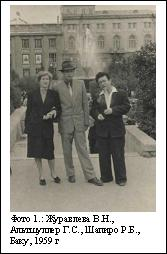
\includegraphics[width=.35\textwidth]{./1.jpg}\vfill
\end{wrapfigure}
Биографов Альтшуллера трудно упрекать в недостаточно тщательном изучении
планов занятий первого курса АзОИИТ (Азербайджанский общественный институт
изобретательского творчества) 1973--74 гг. Как и в том, что они не обратили
внимания на имя человека, фактически подарившего методике понятие технического
противоречия.  Вряд ли справедливо будет упрекнуть и самого Кабанова в
недостаточном участии при создании и разработке новой методики. Но его участие
еще можно представить как выполнение должностных обязанностей.

Особого внимания заслуживает личность Рафаила Шапиро и его вклад в разработку
ТРИЗ и ТРТЛ. Не только потому, что он был другом, ровесником и одноклассником
Генриха Альтшуллера. И не потому, что вместе они создали и запатентовали свои
первые изобретения и написали первые статьи. И даже не потому, что Шапиро
многие годы являлся наиболее близким коллегой-писателем, одним из активнейших
популяризаторов молодой методики. Но, прежде всего, потому, он был одним из ее
основоположников, генератором идей и катализатором творческого процесса. Если
уж многие сравнивают создание ТРИЗ с революцией в изобретательстве, то Шапиро
следует отнести к числу ее пламенных революционеров, незаслуженно вычеркнутых
из исторических разделов учебников.

\begin{quote}
  В 1948--49 гг. непосредственное участие в разработке первых вариантов АРИЗ
  принимал Рафаэль Борисович Шапиро (Р. Бахтамов). Он участвовал также в работе
  на протяжении 1956--59 гг. \cite{Altshuller1974} 
\end{quote}
Другими словами, Шапиро был полноправным соавтором эффективных, лаконичных и
четких вариантов алгоритма -- АРИЗ-56 и АРИЗ-59. Впрочем, в те годы он еще
упоминался в качестве соавтора \cite{Altshuller1956, Altshuller1959}.

Из воспоминаний самого Генриха Альтшуллера можно сделать вывод, что прочность
тандема Альтшуллер-Шапиро основывалась, прежде всего, на значительной
полярности характеров, увлечений, мировоззрений и жизненных целей, которая
притягивала и объединяла двух молодых изобретателей на пути к достижению общих
целей. Годы войны, неудачи первых лет совместного изобретательства, аресты и
допросы, лагерные скитания -- ничто не смогло разделить их, разбить их
духовное единение. Серьезные сложности начались тогда, когда наметились первые
успехи, когда методика начала получать признание. Один из очевидцев этой
неустанной борьбы противоположностей вспоминает: 
\begin{quote}
  Рафик был умнее Альтшуллера. Генрих был ярче, но Рафик был умнее. Он вообще
  был очень умный человек, даже мудрый. Когда он работал в журнале «Страна и
  мир» (мюнхенском издании русских эмигрантов, в котором Шапиро, живший в
  Иерусалиме, многие годы являлся ведущим экономическим и политическим
  обозревателем -- прим. автора), то шутили, что Горбачев принимает решения,
  только прочитав статьи Рафика. Если в журнале издавались две его статьи, то
  одна шла под именем Бахтамова, а другая -- Шапиро.
\end{quote}

Альтшуллер мыслил более конкретными категориями. Работоспособному и
энергичному, ему нравилось действовать, выдавать продукцию, получать
результаты: 
\begin{quote}
  Первое авторское свидетельство на изобретение я получил (совместно с
  Р.Б. Шапиро и И.В. Тальянским -- Л.Ш.)... в школе, когда заканчивал десятый
  класс. После школы я стал студентом Азербайджанского индустриального
  института.  Казалось бы, полученные в институте знания помогут вскоре
  сделать и другие изобретения. Однако прошло много лет, прежде чем мне выдали
  второе авторское свидетельство. За эти годы я отправил 103 заявки на
  изобретения. И получил 103 отказа». \cite{Altshuller1961}
\end{quote}
Альтшуллер был готов перечитывать десятки тысяч описаний изобретений, чтобы
упорно расширять Список Основных приемов (сначала до 50, а затем и дальше) и
стандартов, число параметров в Таблице и т.д.

Шапиро же больше привлекала деятельность, скорее подходящая под определение
грандиозной, гениальной, потрясающей все устои. Именно он явился инициатором
того злополучного письма «товарищу Сталину». Письмо это, к сожалению, до сих
пор не опубликованное, в свое время было разослано более чем в 40 адресов и,
согласно общеизвестной версии, явилось одной из причин многолетнего заключения
обоих друзей в тюрьмах и лагерях. 
\begin{quote}
  У Шапиро возникла мысль написать письмо Сталину. Надо сказать, для него это
  характерная реакция вообще. Когда он проникался сознанием величия чего-то,
  ему хотелось быстро внедрить и получить результат…. Шапиро был потрясающий
  оптимист». \cite{Altshuller1986}
\end{quote}

Информация о создателе ТРИЗ Генрихе Альтшуллере зачастую пересыщена элементами
научно-фантастического и даже героического оттенка, и это не удивительно, ведь
речь идет о биографии профессионального писателя-фантаста.  «В 14 лет он имел
несколько патентов на собственные изобретения. В 20 лет стал профессиональным
патентоведом, экспертом Каспийской флотилии в Баку. Потом он создал новую
науку.»\footnote{Г.С. Альтшуллер, Центральный Еврейский Ресурс.
  \url{http://www.sem40.ru/famous2/e428.shtml}.  2020 no more online -- HGG}.
Так называемым популяризаторам не столь важно, что первая успешная заявка была
сделана с двумя соавторами в 17 лет, а подтверждение пришло двумя годами
позднее. Что больше сотни последовавших за нею заявок были отклонены. Что
«профессиональный патентовед и эксперт», в 20 лет только что бросивший учебу в
институте, «имел все основания считаться крупным авторитетом в области плохих
изобретений» \cite{Altshuller1961}. Что о создании новой науки утверждать,
мягко говоря, преждевременно. Важно, чтобы было красиво.

В подавляющем большинстве исторических справок о ТРИЗ говорится, что письмо
Сталину написал Альтшуллер. Иногда добавляется «вместе с другом». Очень редко
упоминается имя друга. Все же, читая воспоминания Альтшуллера, трудно
отделаться от ощущения, что ему так и не удалось разделить ответственность за
этот поступок поровну: «Я несколько раз отговаривал его (Шапиро, -- Л.Ш.),
когда дело касалось изобретения, а вот здесь...» На этом месте люди, близко
знавшие Альтшуллера и испытавшие на себе сложности его характера, лишь
недоверчиво пожмут плечами. Как, впрочем, и при упоминании других случаев
добровольно-принудительного следования желаниям Рафика Шапиро. Прецедентов
согласия Альтшуллера с чьим-либо мнением, принципиально расходившимся с его
собственным, пока еще никто не припоминал. Тем более, невозможно представить
себе Генриха Альтшуллера в роли исполнителя чужой воли.

Об испытаниях, выпавших на его долю в Бутырской тюрьме и лагерях, о допросах,
на которых его уговаривали признать собственную вину и оклеветать Альтшуллера,
Рафаил Шапиро написал в своих воспоминаниях, уже живя в Израиле. Но так и не
собрался их опубликовать. Лишь спустя два года после его смерти эти записи
были изданы его супругой Норой в небольшой книге «Двадцать пять плюс двадцать
пять». В сумме 50 -- столько должно было исполниться Рафику в день
освобождения в соответствии с приговором суда, который -- по иронии судьбы или
чьему-то «тонкому» расчету -- был оглашен в день его рождения 13-го января
1951 года. Книга, название которой его близкий друг Владимир Портнов,
написавший предисловие, дал уже без него, так и не была закончена. Понимая,
что умирает, Шапиро уничтожил многие черновики и архивные материалы.

Отношение Р. Шапиро к Г. Альтшуллеру и их совместной работе можно было бы
определить, скорее, как трепетное обожание и самоотречение. Вот только один
характерный штрих: В 1961 году Р. Бахтамов (литературный псевдоним Рафаила
Шапиро) издал сборник рассказов «Изгнание шестикрылого серафима», в котором
воспевал заслуги Альтшуллера по созданию новой методики. В том же году Генрих
Альтшуллер в своей книге «Как научиться изобретать» уместил роль Шапиро на
протяжении почти 15-летнего совместного пути в одну строчку, оценив его как
«особенно значительный вклад» в развитие его, Альтшуллера, методики. Впрочем,
и этот вклад Альтшуллер разделил на двоих: Шапиро и Кабанова. По
справедливости.

Было ли случайностью, что работу по непосредственному составлению Таблицы
приемов преодоления технических противоречий, (которую по праву можно отнести
к наиболее трудоемкой, хотя и наименее творческой части усилий по созданию
комплексной методики), Альтшуллер начал лишь после того, как Шапиро
практически «вышел из игры«? А до этого… «Шапиро очень быстро оценил нашу
перспективу… вытекающую сторону. Он сказал так: «Маркс вывел законы развития
общества, Дарвин вывел законы развития живых организмов, \textbf{а мы выведем
  теорию, которая даст миру законы развития технических систем}». …То есть он
первый оценил эту штуку, это очень важно. Масштаб ее понял»
\cite{Altshuller1986}.  Эти слова Альтшуллера появились не в его книгах или
статьях, и не в 1961 или 1965. Вклад Шапиро был оценен по заслугам лишь в 1986
году при записи мемуаров Альтшуллера в частной беседе с одним из его учеников.

С уходом Шапиро из общего дела по времени совпадает и увлечение
Г.С. Альтшуллера идеей создания «Эвротрона» (первой механической
«изобретающей» машины, как ее представляет Фонд Г.С Альтшуллера). Об этой
истории нам известно пока очень мало. Зато достаточно очевидной представляется
каталитическая роль «Эвротрона» в появлении на свет Таблицы
противоречий. Механический изобретатель требовал и легко жующегося
«механического» питания.

В общем, если отвлечься от революционной тематики и признать Альтшуллера
полноправной «матерью» ТРИЗ, выходившей и воспитавшей ее, (то есть по-прежнему
считать, что «родил» методику именно он), то Шапиро, скорее, был ее духовным
отцом, покинувшим семью в пубертатный период их общего ребенка и вскоре
лишенным прав отцовства.

Лишь через два года после смерти Шапиро -- в канун своего 70-летия --
Альтшуллер впервые называет некоторые даты, касающиеся бывшего соратника и
друга: 
\begin{quote}
  \textbf{Шапиро Рафаэль Борисович} (литературный псевдоним -- Бахтамов Р.Б.)
  присоединился ко мне в 1942 году (когда Генриху было 16 лет, -- Л.Ш.),
  вместе кончили десятый класс, вместе пошли на нефтемеханический факультет
  Азербайджанского индустриального института. Первое зарегистрированное
  изобретение -- тоже общее. И срок отсидки в ГУЛАГе тоже нам отмерили поровну
  -- по 25 лет. Выпустили нас тоже в один день -- 23 октября 1954 года.
  Освободившись, Шапиро проработал в ТРИЗ по 1961-й год. Ушел из жизни в 1994
  году.  \cite{Altshuller1996}
\end{quote}
Совместная работа над разработкой ТРИЗ ушла в прошлое, но бывшие соратники еще
не расстались. Теперь уже под псевдонимами писателей-фантастов они продолжали
спорить о путях развития методики творчества. Именно в рассказах и повестях
Г. Альтова и Р. Бахтамова можно наиболее последовательно проследить
становление личностей и мировоззрения этих наиболее значительных
основоположников ТРИЗ.

\begin{quote}
  Перегнать науку тяжело, -- говорит писатель Р. Бахтамов. … Пусть не обидятся
  на меня товарищи по перу, но, на мой взгляд, предметом
  научно-фантасти\-ческой книги должна быть не техническая проблема, а, прежде
  всего человеческие идеи, человеческие проблемы, короче, человек будущего
  мира.  Тогда это будет настоящая литература.

  Альтов, возражая Бахтамову, добавляет:

  Но для того, чтобы сказать о будущем человеке, нужно сказать, где он живет,
  в каком мире. И от того, как мы развиваемся, как мы идем к этому будущему
  миру, от того, каков технический прогресс -- от этого зависит, каким показать
  человека. …

  Р. Бахтамов написал новую книгу «Властелин оксимира». Фантаста увлекла
  человеческая идея: что будет с таким качеством, как героизм, если его не
  нужно будет проявлять? \cite{Amnuel964}
\end{quote}
Возможно, что принципиальные разногласия писателей Р. Бахтамова и Г. Альтова
во взглядах на развитие научно-фантастической литературы сыграли свою роль в
том, что имя Шапиро на многие годы практически перестало упоминаться в
материалах по ТРИЗ.

Как бы там ни было, но Рафик Шапиро сошел с дистанции, подобно многим другим.
А Альтшуллер остался и продолжил работу. На протяжении полувека именно он
являлся организатором и координатором, связующим звеном, аккумулятором
информации и движущей силой общего процесса, который сегодня уже традиционно
воспринимается последователями как «создание ТРИЗ». Уже поэтому тот сгусток
идей, опыта, но и неизбежно наработанных стереотипов, который мы называем
«классической ТРИЗ», это в значительной степени и его увлечения, гениальные
идеи и отчаянные заблуждения. Это и победы Альтшуллера над собственной
инерцией мышления, свойственной гениям в не меньшей степени, чем их
предшественникам и современникам, только, быть может, распознаваемые на
значительно более высоком уровне. Это и его ошибки, в которых ему так нелегко
было признаться даже самому себе, от которых было так трудно, порою просто
невозможно, отказаться. Ошибки тем более обидные, что они потребовали многих
лет жизни -- сначала для их созидания, а после -- для исправления или
«забывания». Отдавая дань гению Альтшуллера, мы все же не обязаны слепо
следовать и его гениальным ошибкам, маскируя их под достижения в трепетном
стремлении сохранить лицо и укрепить авторитет Учителя. Не признавать ошибки
-- значит, создавать новые, все более дорогостоящие и трудно исправимые.

Важно подчеркнуть, что ТРИЗ -- это наиболее успешная, но не завершенная
попытка привести в систему все многообразие мыслительных механизмов многих
поколений изобретателей, которые кропотливо и настойчиво собирал, развивал,
проверял и использовал на протяжении своей жизни Генрих Саулович Альтшуллер.
Поэтому методика образца 80-х во всем ее многообразии отражает, прежде всего,
динамику развития личности, процессов мышления и изменения взглядов на эти
процессы самого Альтшуллера. Известны лишь немногие отдельные случаи признания
им каких-либо значительных изменений или дополнений, предлагавшихся более
юными последователями. В частности, Альтшуллер долгое время настаивал на своей
неограниченной монополии на «производство» и развитие АРИЗ.

ТРИЗ не является законченной «методикой поиска новых идей» для всех и каждого,
но скорее трафаретом, образцом, набором кубиков-элементов, с помощью которых
каждый может скроить себе свою систему развития талантливого мышления на
основе исходных установок, собственного жизненного опыта, сложившихся
стереотипов и поставленных задач. Теоретически «законченной» она могла бы
стать для ее авторов. Но с уходом Альтшуллера развеялась последняя надежда и
на это. Незавершенными останутся Общая теория сильного мышления (ОТСМ) и
Теория развития творческой личности (ТРТЛ). Создание Теории Сильного Мышления
преобразовалось в некую надсистемную Достойную Цель, столь же идеальную, сколь
недостижимую в рамках жизни отдельно взятой личности или одного поколения. И
неспроста серьезное изучение ТРИЗ неизбежно перекликается с осмыслением
истории ее создания.

ТРИЗ как методика, основанная на синтезе приемов и алгоритмов, отражает модели
мышления, свойственные различным творческим личностям в самые разные периоды
их жизни и деятельности. Именно это обстоятельство объясняет тот факт, что
даже опытные и заслуженные специалисты не используют, не воспринимают, а порой
и отвергают отдельные элементы ее инструментария. Нередки случаи стихийного
«переосмысливания», наивного упрощения отдельных элементов, вынужденного
возврата к уровню 30-40-летней давности. С другой стороны, некоторые операторы
и приемы, даже сам АРИЗ, порой дополняются и развиваются энтузиастами из числа
«новых тризовцев». Эти представители коммерциализированного поколения зачастую
даже не имеют понятия о том, что этот путь однажды (а то и не раз) уже был
пройден другими.

Но вернемся к нашим табличным вопросам.

\subsection*{Таблица умножения современного изобретательства?}

Авторами многих публикаций об использовании методики и рекламных объявлений
являются,согласно аннотациям, опытные ТРИЗ-специалисты с многолетним стажем
практической работы. Какие же инструменты-кубики выбирают для себя современные
последователи и «разработчики» ТРИЗ на Западе? Отчего порой в качестве
универсальных средств предлагаются сомнительные, морально безнадежно
устаревшие инструменты? Так в большинстве материалов речь идет о
\textbf{Таблице приемов устранения технических противоречий} (далее --
\textbf{Таблица}) и традиционно относящихся к ней 40 приемах их преодоления.
На Западе она известна больше как «\textbf{Матрица противоречий}»
(Widerspruchsmatrix, Contradiction Matrix), на Востоке как «\textbf{Таблица
  умножения}». С середины 90-х по сей день, она остается излюбленным и
наиболее известным, чаще других упоминающимся и успешно используемым
«инструментом» ТРИЗ. Интернет пестрит сообщениями и рекламными объявлениями,
подобными приведенным ниже (Вставка А).

С легкой руки российских экспортеров ТРИЗ и американских, а затем европейских
любителей изобретательства Таблица в буквальном смысле пошла по рукам.
Сногсшибательный эффект от ее использования обнаруживают специалисты в самых
разных областях деятельности. Наиболее свежими членами «Клуба любителей
Таблицы» стали бизнесмены \cite{Leon2005}, архитекторы \cite{Mann2005a},
музыканты \cite{Mann2005b} и банкиры \cite{Stuart2005}. В очереди на прием в
Клуб стоят массажисты, диск-жокеи и стоматологи.

Сегодняшняя ситуация в Европе отдаленно напоминает положение вещей в СССР
60-70-х годов, когда молодая методика с большим трудом пробивала себе дорогу в
ученых и бюрократических кругах. Таблице, благодаря математической стройности,
внешней простоте и убедительности, удалось в те годы примирить многих ярых
противников методики с фактом существования ТРИЗ.

Но метаморфозу, происходящую с ТРИЗ в Европе начала 21-го века трудно назвать
развитием. Скорее, это неуклонное упрощение и стремительная деградация
классической методики с постепенным распадом на отдельные наглядные и легко
продаваемые «кирпичики». В наши дни у нее появляется все больше сомнительных
друзей и почитателей, стремящихся переиначить и перекроить ее. Попытки
компенсировать кажущуюся им сложность ТРИЗ или непонимание отдельных ее
инструментов достигаются путем самых различных «обрезаний», созданием новых
«упаковок» и псевдоалгоритмов. Лишь за последние годы появились варианты
«упрощенной» ТРИЗ: Meta-TRIZ, TriSolver-ARIZ, SIT (Систематическое
Инновационное Мышление), ASIT (Передовое СИМ), USIT (Универсальное СИМ) и
другие. Появление подобных мутантов, казалось бы, должно мобилизовать
последователей Альтшуллера на организованную защиту методики и своих рядов.
Вместо этого все большее число тризовцев попадают под знамена новоявленных
«модернизаторов». Вырвавшись из-под «железного занавеса» бывшей тризной
империи, методика растеряла большую часть своей изначально романтической
мотивации и превратилась в расхожий товар. Европа вступает в эпоху Т-ТРИЗ --
Табличной ТРИЗ.

Декларируемое назначение Таблицы -- облегчить, как для начинающего
пользователя, так и для опытного решателя выбор приемов разрешения типовых
противоречий для решения конкретной задачи. Ставшая в Европе символом ТРИЗ,
громоздкая и труднообозримая Таблица, в действительности, не только в
значительной степени усложняет и удлиняет поиск решений, но зачастую
окончательно заводит пользователя в тупик, исключая возможные решения целиком
из поискового поля.

Уже в период своего создания Таблица фактически не являлась работающим
инструментом. А ведь именно благодаря массированному применению Таблицы и
изобретательских приемов, ТРИЗ в последние годы все чаще приравнивают к
«структурированному мозговому штурму». Внешне четкий и наглядный инструмент,
Таблица вкупе со Списком Основных приемов содержит в себе множество острых
противоречий, основополагающих заблуждений, сводящих даже теоретические
возможности ее использования для целенаправленного решения технологических
проблем к нулю.

Предпринимаемые в последнее время все чаще попытки представить ТРИЗ как некую
панацею при любых недугах технического или социального характера, в
значительной мере вредят как самой методике, ее развитию и распространению,
так и ее носителям -- ТРИЗовцам. За этими попытками в большинстве случаев
стоит все та же Таблица противоречий! И если для 90\% технарей, знающих о
методике понаслышке, Таблица является ее символом, то для большинства знатоков
она олицетворяет или ее вчерашний день, или ее сегодняшнюю деградацию и
стремительный развал тризного движения, некогда представлявшего собой
изысканное сообщество интеллектуалов.

Предлагаемая серия статей предостерегает, прежде всего, промышленных
заказчиков и начинающих пользователей методики от поспешности при выборе
инструментария. Это и призыв к осмотрительности, как при заключении договоров
на оказание консультационных услуг, так и в вопросах приобретения программных
продуктов на базе ТРИЗ, предлагаемых сегодня на европейском рынке. Статьи
содержат многие малоизвестные факты из истории создания методики и отдельных
ее элементов, в том числе «постоянного и полномочного представителя» --
Таблицы технических противоречий. Сопоставление фактов и цифр наглядно
демонстрирует несостоятельность Таблицы как рабочего инструмента в целом, так
и как вспомогательного механизма для интенсификации поиска решений для
несложных проблемных ситуаций в частности. Становится очевидной и
необоснованность выбора ее в качестве информационного фонда при создании
ТРИЗ-базируемых программ для «изобретающих машин», что ставит под вопрос
практическую значимость и эффективность использования большей части
компьютерных «изобретающих» программ и их составляющих, предполагающих в любой
форме применение Приемов на основании «табличных» рекомендаций.

В «\textbf{Проекте требований для оценки уровня подготовленности заявителей
  при аттестации в МА ТРИЗ}» \cite[Приложение 2]{MATRIZ2003} большое внимание
уделено следующим вопросам:
\begin{itemize}
\item 2 уровень; Знать основные блоки истории ТРИЗ, как науки -- таблицу и 40
  приемов преодоления технических противоречий, основные этапы развития АРИЗа.
  Иметь представление о дополнениях или изменениях, внесенных другими
  специалистами по ТРИЗ. Уметь оценивать уровень и инструментальность этих
  изменений.
\item 3 уровень; Знать ход развития ТРИЗ, основные изменения в теории, начиная
  с первых публикаций, понимать причины и закономерности этих изменений.
\end{itemize}
Предлагаемые материалы рассчитаны, таким образом, и на всех желающих
приобрести сертификат 2-го, 3-го уровня и выше -- вплоть до «Мастера ТРИЗ».

\subsection*{Вставка А: Таблица приемов преодоления технических противоречий в
  Интернете} 

«ТРИЗ предлагает быстрый и целенаправленный поиск решений, помогает
классифицировать техническое противоречие с помощью параметров и основных
приемов целевым порядком». Martin Fritz (Universitat Stuttgart) предлагает
дополненную Таблицу противоречий в своей работе «Потенциальный анализ
относительно объединения методов ТРИЗ и бионики» по цене EUR
24,99\footnote{\url{http://www.hausarbeiten.de/faecher/vorschau/39753.html}}.

«Снижение себестоимости при помощи Таблицы противоречий» обещает Thomas
Schlos\-ser\footnote{\url{http://www.triz-online-magazin.de/ausgabe03_03/artikel_4.pdf}}.

Таблица противоречий предлагается при использовании Изобретательского Решения
проблем в Requirements
Engineering\footnote{\url{http://www.fb9dv.uni-duisburg.de/se/de/education/ws0405/RE/SaschaBrink(2004)SemRE-TRIZ.pdf}}.

«В основе всех технических решений лежат 40 так называемых изобретательских
приемов. Через выявление противоречий в системе может быть проведен
целенаправленный поиск решений». «Таблица противоречий, как известнейший из
инструментов ТРИЗ, и относящиеся к ней абстрактные шаги» рассматриваются в
серии семинаров
\textbf{SUPPORT}\footnote{\url{http://www.stenum.at/download/folder_support.pdf}}.

«Одним из самый известных инструментов ТРИЗ-методики является Таблица
противоречий», хвалит Dr.habil.oec.Dipl.-Ing. Petra Rietsch. Применение
Таблицы при создании нетехнических новшеств можно изучить на семинаре «Анализ
деловых моделей е-бизнеса малых и средних
предприятий»\footnote{\url{http://www.wu-wien.ac.at/kmb/lehre/sbwlneu/vk52}}.

Преимущества и недостатки \textbf{Таблицы} сравнивает \textbf{INVENTNET® GmbH}
на своей
странице\footnote{\url{http://www.inventool.de/toolauswahl/tooldescription.php?id=123}}.

«В особенности, начинающим ТРИЗовцам рекомендуются 40 изобретательских приемов
для преодоления технических противоречий и система их применения в форме
Таблицы противоречий как инструмента для легких и средней тяжести
изобретательских задач («Свободная Обучающая Платформа для изобретателей и
разработчиков«). Работа с приемами здесь начинается с 10 лучших принципов для
мозгового штурма\footnote{\url{http://www.triz.it/ebf/tct03.htm}}.

Johannes Maierhofer (Future Management) представил на 4. Конгрессе ТРИЗ
анализ, в котором в качестве «лучших» методов, соответствующих требованиям
новаторского проекта, были признаны QFD, системный анализ процессов и Таблица
противоречий, поддерживаемые программой Logic Mind
Guide\footnote{\url{http://www.triz-online.de/triz_magazin/ausgabe05_03/artikel_5.htm}}.

\clearpage
\begin{flushright}
  «Сейчас 40 приемов имеют лишь историческое значение«\\
  Г.С. Альтшуллер \cite{Altshuller1985}
\end{flushright}
\section*{2. Самый главный инструмент!}

По окончании моего доклада на 4-м Конгрессе ТРИЗ (Frankfurt/Main, 30.06.2005)
мне было задано несколько вопросов. Два из них звучали (в переводе на русский
язык) так: «Работая в проекте, Вы анализируете задачу, формулируете
техническое противоречие, выбираете по Таблице приемы, а дальше?» После моего
замечания о том, что Таблица не является инструментом для решения
производственных задач, и я не пользуюсь ею, а Альтшуллер уже 30 лет назад
придавал ей лишь историческое значение, в зале возникло тягостное молчание.
Чувствовалось, что сидевшие в зале участники были шокированы ответом. Вопросов
мне больше не задавалось. Не о чем было спрашивать! Ну, в самом деле, о чем
можно говорить с человеком, не использующим в работе Таблицу?!

Вот так у меня появился повод разобраться с феноменом «Таблицы приемов
преодоления технических противоречий». А заодно и окончательно выяснить для
себя смысл ее существования. Уж не пропустил ли я за 20 лет, прошедших с
последнего учебного семинара, какие-то революционные разработки в этом
вопросе? Уже просматривая странички в Интернете, восхваляющие «подзащитную», я
понял, что гораздо эффективнее будет сделать харакири под плакатом
«\textbf{НЕТ -- Таблице!}» на очередной Конференции ETRIA в Граце, чем
пытаться обратить «мирным путем» внимание европейской тризной общественности
на существование (вернее, фактическое отсутствие) проблемы. (Собственно, этим
теперь и приходится заниматься).

\begin{center}
  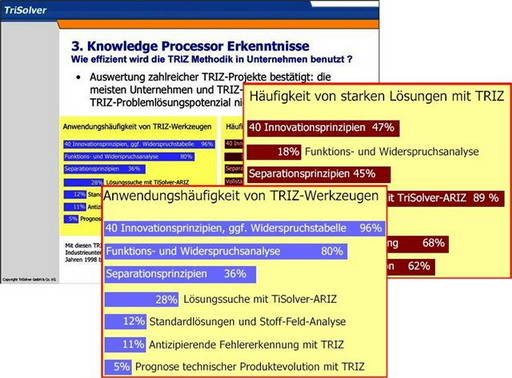
\includegraphics[width=.8\textwidth]{./2.jpg} \\
Рис. 1. Частота применения инструментов ТРИЗ фирмой TriSolver\\ и их успешность
в 1998--2005 годах (на опыте работы с 38 предприятиями)
\end{center}

В докладе консультационной фирмы TriSolver «Новаторство как процесс» на этом
же Конгрессе \cite{Livotov2005} (материал снят с сайта!)  предлагается
сравнительный анализ частоты использования и эффективности наиболее
значительных инструментов ТРИЗ по результатам многочисленных проектов,
проведенных этим консалтингом в 1998--2005 годах на 38 промышленных
предприятиях Европы (Рис. 1). В большинстве своем это известные и уважаемые
имена, многие из которых (DaimlerChrysler, Philips Semiconductors, Infineon
Technologies, Siemens Dematic и др.) названы на сайте
фирмы\footnote{\url{http://www.trisolver.de/software/innovationssoftware.htm}}.

«Таблице противоречий и 40 изобретательским приемам» (40
Innovationsprinzipien, ggf. Widerspruchstabelle) отводится в этом реестре
абсолютное первое место по уровню симпатий клиентов. С 96\%-ой частотой
используются они в проектах, проводимых TriSolver! Убедительно лидируя среди
коллег-инструментов, Таблица значительно опережает функциональный анализ
(Funktions- und Widerspruchsanalyse, 80\%) и выглядит совсем недостижимой для
таких «мало востребованных» инструментов, как принципы разделения физических
противоречий (Separationsprinzipien, 36\%) или вепольный анализ, включая
стандарты (Standardl\"osungen und Stoff-Feld-Analyse, 12\%). Даже поиск
решений с участием «фирменного» \textbf{TriSolver-ARIZ} (значительнее звучала
бы разве что только «TriSolver теория относительности«) занимает с 28\% лишь
четвертое место по важности. Старушке Таблице удалось переплюнуть по частоте
использования всю замыкающую список пятерку инструментов, включая
прогнозирование и «диверсионный анализ» (AFE).

В половине случаев (47\%) применения Таблицы и приемов специалистам фирмы
удается -- следуя диаграмме -- получить «сильные» решения. Хотя выход таких
решений пока еще на 40\% ниже, чем при решении проблем по TriSolver-ARIZ,
общее количество их для Таблицы при ее практически повсеместном использовании
все же в два раза перекрывает результаты, достигаемые алгоритмом, и в три раза
-- принципами разделения физических противоречий. Успехи вепольного анализа на
фоне «табличных» заслуг выглядят просто смехотворными.

Фирма TriSolver является, по утверждению ее представителей, ведущей на
немецкоязычном рынке по оказанию консультационных услуг и разработке
компьютерных программ в области ТРИЗ и системного новаторства. Было бы логично
предположить, что эта фирма прилагает все усилия для популяризации методики
(как в целом, так и отдельных ее инструментов) в различных отраслях
промышленности, расширяя и развивая свой собственный арсенал. В
действительности же, почти все приведенные в диаграмме «классические»
инструменты потеряли только за один год от 30\% до 50\% пользовательского
спроса (Рис. 2). Все, кроме Таблицы!

\begin{center}
  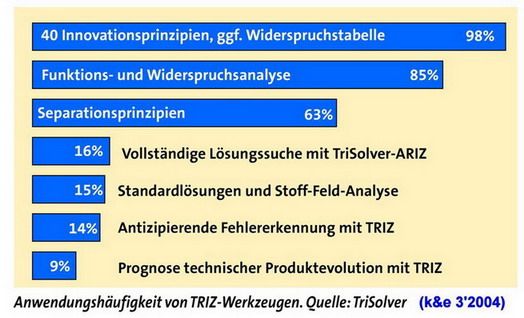
\includegraphics[width=.8\textwidth]{./3.jpg} \\
  Рис. 2. Частота применения инструментов ТРИЗ фирмой TriSolver в 2004 г.
  (Konstruktion \& Engineering, 03/2004).
\end{center}

Особенно примечательным является тот факт, что еще годом раньше принципы
преодоления (разделения) физических противоречий востребовались клиентами
TriSolver в два раза чаще (63\%)! И только применение \textbf{TriSolver-ARIZ}
имело в 2004 году еще более эпизодическое значение, чем нынче -- лишь 16\%. Об
этом говорилось в фирменном отчете о Конференции ETRIA-2004 в
западногерманском городе Aachen \cite{Livotov2004}.

Абсурдной динамика изменения (перераспределения) удельной частотности
использования элементов ТРИЗ в работе TriSolver представляется лишь на первый
взгляд. Она становится значительно понятнее после знакомства с основными
принципами действия единственной на сегодняшний день немецкоязычной программы
\textbf{TriSolver4.net}. В основе ее лежат, конечно же, тризные рекордсмены:
Таблица и 40 основных приемов!

Таким образом, вытеснение интеллигентных и эффективных, но требующих
повышенных затрат времени при обучении (и уже только по этой причине менее
привлекательных) инструментов «универсальной» Таблицей приобретает воистину
промышленные масштабы. Эта тенденция становится все более заметной как у
отдельных консультантов, так и у индустриальных пользователей ТРИЗ, обретая
черты диагноза. А ее лавинообразное ускорение, пусть не всегда такое
драматичное, как у \textbf{TriSolver}, заражает азартом соседей по рынку
консультационных услуг.

Вот выдержка из статьи, с которой имели возможность ознакомиться более 5
миллионов читателей немецкого «Шпигеля» от Канарских островов и «до самых до
окраин» -- Японии и Гонконга: «Томас Байер, шеф исследовательского отдела
фирмы Виттенштайн, держит список 40 приемов постоянно перед глазами. В его
бюро они висят на стене рядом с Таблицей, которая помогает ему выявить, какое
из правил подходит к той или иной дилемме» \cite{Dworschak2005}. Подобного
рода «ненавязчивая реклама» все чаще появляется как в технической и
научно-популярной прессе, так и в крупных информационных журналах. Европейцы
еще не забыли, что и другая, не менее важная таблица химических элементов
пришла когда-то с морозного Востока -- а ведь и в ней тоже были незаполненные
клетки! Этот аргумент убеждает.

\begin{center}
  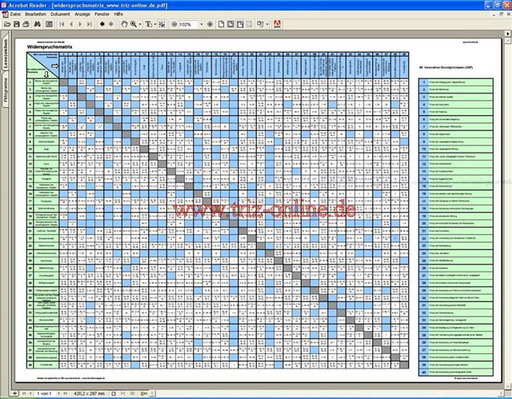
\includegraphics[width=.8\textwidth]{./4.jpg} \\
  Рис. 3. «Классическая» Таблица приемов преодоления технических противоречий
  (АРИЗ-71). Голубым цветом выделены пустые клетки.
\end{center}
Опубликованная на сайте журнала triz-online (Рис. 3) наиболее точная немецкая
версия Альтшуллеровской Таблицы в ее «классической» форме копируется
многочисленными почитателями и знатоками этой части методики в Европе.

Что же это за универсальный инструмент изобретателя, которому с 1998 по 2005
годы отдавали абсолютное предпочтение 38 промышленных предприятий и фирм --
преданные клиенты TriSolver? Мощный инструмент изобретательского мышления --
памятник гению Альтшуллера? Увлекательный калейдоскоп, в котором при каждом
повороте возникают новые занятные сочетания? Забавная игрушка для прожектеров,
помогающая генерировать как явно сумасшедшие, так и сногсшибательно
правдоподобные идеи?

\begin{center}
  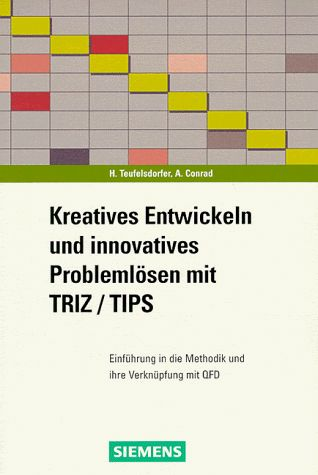
\includegraphics[width=.5\textwidth]{./5.jpg} \\
  Тризная геральдика
\end{center}
В качестве иллюстрации к обложке одного из первых немецких изданий по
TRIZ/TIPS \cite{Teufelsdorfer1998} была выбрана стилизованная Матрица. Именно
она все чаще выдается западными консультантами за «почти всю» ТРИЗ или, по
крайней мере, за ее основной, наиболее четко и безотказно действующий
универсальный механизм. Их утверждения, по крайней мере, статистически не
лишены оснований. У постоянно растущего числа людей разных профессий и
вероисповеданий, национальностей и цвета кожи «русская» методика
изобретательства ассоциируется именно с нею. Если провести опрос всех
европейцев, когда-либо слышавших о ТРИЗ, и поинтересоваться тем, какой образ
рождается в их воображении при ее упоминании, то в 99\% случаев будет получен
контрольный ответ. А вот горящая в голове лампочка Ильича, в России нередко
используемая как символ творческого изобретательского мышления, вызывает у
западного читателя скорее болезненные ассоциации. Роденовский мыслитель,
отдавший за идею последнюю рубашку, тоже не возбуждает: С положениями ЖСТЛ на
вводных и обзорных семинарах не знакомят -- эти материалы упрямо не поддаются
адекватному переводу ни на один европейский язык. Зато Таблица понятна и без
перевода.

Действительно, свобода формулировать многочисленные противоречия с получением
самых причудливых конфликтных пар создает видимость расширенного, хотя и
поверхностного «вылавливания» идей. Именно последнее обстоятельство превращает
применение Таблицы внешне похожим на «офилософствованную» и несколько
систематизированную помесь перебора вариантов с мозговым штурмом. И создает из
нее легко уязвимую мишень для вдумчивых и технически хорошо образованных
критиков. Оно же дает повод убежденным противникам «коммунистических» методов
мышления огульно распространить слабости Таблицы на все остальные инструменты
ТРИЗ. Всякое упоминание о ее диалектических основах и без того вызывает у
простых капиталистов аллергическую реакцию, напоминая о неизбежной
необходимости разрушения всего (их) мира до основанья.

Таблица открыла новую эру в развитии и распространении ТРИЗ на Западе.
Методика в ее лице начала превращаться в продукт изобретательского ширпотреба.
Глубокое и вдумчивое изучение философских основ стало необязательным, как
правило, невозможным, а зачастую и вредным. Все более второстепенное значение
приобретают «громоздкие» варианты последних АРИЗов. Владение Таблицей и
приемами, подкрепленное дюжиной смачных примеров, позволяет увлечь
потенциального клиента ошеломляющей идеей «целенаправленной дистилляции
конфликтующих влиятельных характеристик при изменениях в системе»
\cite{Sietmann2001}. 

Редкий «ТРИЗ-специалист» в Германии рискнет прийти на деловую встречу без
тщательно выглаженной и аккуратно сложенной Таблицы в кармане пиджака. Потому
что если без Таблицы, то каждому ясно, что это -- не специалист. Если
проследить динамику распространения методики в мире, то крамольная мысль об
обратной зависимости среднего уровня владения тризным инструментарием от
общего числа пользователей напрашивается сама собой.

\begin{center}
  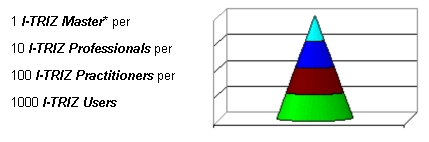
\includegraphics[width=.5\textwidth]{./6.jpg} \\
  Рис. 4. Тризная
  иерархия\footnote{\url{http://www.ideationtriz.com/training.asp}}. 
\end{center}

Воспользовавшись выявленной специалистами Ideation International Inc.
пропорцией между числом простых и непростых пользователей ТРИЗ,
Г.С. Альтшуллер легко определил размеры популяции передовиков
изобретательства. В 1998 году их -- от новичков до Мастеров ТРИЗ -- было чуть
больше 70 тысяч. Обвинять всех Мастеров (на диаграмме -- голубые) в ежедневном
и повсеместном использования Алгоритма было бы неосторожным. Зато вычислить
число абсолютных знатоков Таблицы (зеленые) не составляет труда.

В России 60-х годов она не только олицетворяла собой научный (статистический)
подход в изобретательской деятельности, но еще и играла важную политическую
роль в процессе официального признания ТРИЗ. Идея ее создания была для
Альтшуллера удачной находкой, позволяющей совместить декларируемую точную
алгоритмизацию изобретательского процесса с возможностью использовать богатые
внутренние информационные ресурсы решателя. Она же помогала порой избегать
необходимости расшаркиваться перед инертными теоретиками изобретательства
до-ТРИЗной эпохи. Далеко не все были готовы отказаться от милого сердцу МПиО с
его романтичными, окутанными в золотое вспышками внезапного, но заслуженного
озарения. Кто-то просто боялся высовываться. Ведь не случайно официальная
позиция науки на этот счет десятилетиями практически не развивалась:
«Показательны в этом отношении статьи, опубликованные в N2 журнала
«Изобретатель» за 1929 г. (учитывая, что в период 1937-45 других работ по
психологии изобретательского творчества не появлялось, можно считать, что
взгляды, существовавшие в 1929 г., сохранили силу и к 1946 г.)»
\cite{Altshuller1975}.  О том, что многие сторонники «других взглядов» были
элементарно уничтожены, говорить вслух в 1975 году было еще не принято. Но не
знать этого Альтшуллер, сам прошедший тюрьмы и лагеря, не мог.

Едва появившись на свет, Таблица попала на благодатную почву, словно
специально для нее подготовленную. Советской стране требовались тысячи новых
технических решений. Прежде всего, речь шла об улучшении устаревших механизмов
и дальнейших разработках практически во всех отраслях промышленности.
Поскольку уровень таких инноваций вовсе не обязательно должен был быть
чересчур высоким, -- предпочтительнее были как раз не слишком сложные, но
оригинальные решения, -- приветствовалось быстрое и относительно недорогое
«претворение в жизнь». Поэтому заключенный в строгие табличные формы механизм
«разогрева» инженеров, дающий возможность в непринужденной обстановке одним
стимулировать, а другим симулировать выход на развивающие идеи, пришелся ко
двору.

«Приемы изобретательства были известны и до Г.С.Альтшуллера. Но у него они
были классифицированы (таблица из 40 приемов решения техпротиворечий) и
радикально изменены по структуре» \cite{Murashkovsky2003}. Таблице
удавалось, за счет подкупающей свежести некоторых приемов, соблазнять технарей
необычностью способа интенсификации перебора вариантов. Разложенные по Таблице
в убеждающе неравномерном порядке, приемы играли роль морковок, к которым надо
было тянуться. Волей-неволей приходилось напрягать мозги. В зависимости от
числа сформулированных технических противоречий и уровня общей эрудиции
«тянущихся», таких морковок набиралось от двух-трех до дюжины.

Сегодня лишь небольшая часть коммерческих пользователей ТРИЗ открыто признает
необходимость полного и окончательного отказа от практики одурачивания
клиентов «Гаданием по Таблице». \textbf{Чем же тогда?} -- резонно возражает
значительная масса тризовцев. Но и рьяные сторонники табуляции разделяются на
две конфронтирующие партии: ортодоксов и реформаторов.

По благоговейной тщательности, с которой изобретатели разных стран и народов
оберегают целомудренность Альтшуллеровской Матрицы образца 1971 года,
аккуратно расставляя священные числа от 1 до 40 в нужные клеточки и не
расставляя в ненужные, их можно сравнить, пожалуй, лишь с Хранителями древнего
Пятикнижия. Так приверженцы Кабалы свято верят в божественное происхождение
библейских свитков. Всякое изменение буквенной последовательности, по их
мнению, не только меняет смысл текста, но и приводит к безвозвратной потере
зашифрованных в гигантском буквенном ребусе пророчеств и предначертаний.
Поклонение тризовским скрижалям, включая богослужения перед образами Таблицы с
соблюдением предписанных обрядов, на Западе имеет все шансы перерасти в
устойчивую изобретательскую религию. Читая тут и там об удивительно
целенаправленном и результативном выборе судьбоносных приемов, невольно
вспоминаешь анекдот, в котором старый фельдшер, разламывая пополам таблетку
анальгина, наставлял больного солдата: «Это тебе, сынок, от головы, а это от
живота! Только смотри, не перепутай!» Смешно? Оборот от внедрения анекдота в
производственную практику достиг в последние годы астрономических сумм,
заставляющих подавить усмешку.

«В принципе, можно ткнуть, не глядя, в любой прием, и уже что-нибудь удается
придумать», -- мнение Мастера ТРИЗ Исаака Бухмана поддерживают многие «старые
волки», познавшие бессмысленность Таблицы еще в советские времена.
Бессмысленность, но не бесполезность!

Действительно, тыкать вслепую в список из 40 приемов для обученного (тем
более, сертифицированного) специалиста как-то несолидно. А перебирать их (с
подприемами -- больше сотни) по очереди -- лженаучно! Другое дело -- тыкать в
Таблицу с четырьмя тысячами счастливых номеров, подчиняющимися строгим
статистическим законам, «по науке». Это уже -- профессия!

Особенно плотно смыкаются ряды борцов за «истинную, неделимую и нерушимую»
перед лицом то и дело возникающей опасности со стороны всевозможных
ревизионистов и реформаторов, упорно пытающихся расширить, дополнить,
начистить и раскрасить до боли родную Таблицу 1971 года. Впрочем, до крестовых
походов дело не дойдет. Ситуация, как и положено, подчиняется главному
диалектическому закону -- единству и борьбе. Борьба за истинную веру затмевает
единство принципиального вопроса -- а был ли мальчик? Являлась ли Таблица
вообще когда-то работоспособным и обоснованным инструментом?

Всякий хорошо воспитанный тризовец знает, что к любым утверждениям «классиков»
следует относиться с уважением -- не суть важно, идет ли речь, к примеру, о
пяти тысячах или же двух миллионах изученных патентных документов. Но ведь и
отделять фантастику от реальности в Союзе тоже когда-то учили. Для этого и
инструмент был разработан соответствующий -- Регистр фантастических идей.

Но европейские тризные миссионеры с Регистром не знакомы. Мощь табличного
оружия здесь принимается на веру и традиционно обосновывается
умопомрачительным числом «сильных» решений, легших в его основу. Три четверти
западных популяризаторов ТРИЗ демонстрируют это могущество, словно
сговорившись, на одном и том же примере: Решение задачи об упаковке пиццы,
полученное для американской фирмы Pizza-Hut, приписывается применению
Таблицы. «Альтшуллер идентифицировал на основе изучения 2.5 миллионов патентов
39 технических параметров и 40 изобретательских приемов… А хорошие идеи не
валятся с неба», проповедует Rolf Herb слушателям своего семинара. Добрую
половину интервью для немецкого журнала «Wirtschaftswoche» («Экономическая
Неделя«) он посвящает восторженному разбору этого основательно приевшегося
даже в Европе решения\footnote{Kind im Manne, Wirtschaftswoche Nr.19,
  4.5.2003}.

Другой активный популяризатор Альтшуллеровской методики, ответственный за
обмен технологиями в торгово-промышленной палате земли Хессен и активный
организатор Конгресса во Франкфурте Carsten Gundlach «разжевывает» историю с
Pizza-Hut уже под голландским соусом\footnote{C. Gundlach. Mit Kreativität und
  Strategie zur Nachhaltigkeit. TRIZ Online Magazin 05/2003, no more online --
  HGG.}. Невольно возникает ощущение, что остальные пять примеров,
переведенные из российских и американских книг, не жуются.

Читая в западных источниках об \textbf{огромном}, \textbf{гигантском} или
\textbf{необъятном} патентном фонде, переработанном Альтшуллером при
составлении Таблицы в 1946-65 годах, как и о «доработанных» позднее его
учениками двух или четырех миллионах патентов (с целью подтверждения указанных
в ней приемов), невольно вспоминаешь другой анекдот. О сапожнике, соседями
которого по переулку оказались «лучший в городе» и «лучший в стране»,
повесившем у своей будки табличку «Лучший на этой улице». Чтобы окончательно
закрыть вопрос об объемах учтенной информации, остается лишь заменить термины
местного масштаба «огромный» или «гигантский» на скромный, но со вкусом --
«ВЕСЬ мировой патентный фонд».

\subsection*{Таблица умерла! Да здравствует Таблица!}

К началу 70-х в СССР позиции ТРИЗ стали настолько устойчивыми, что
Г.С. Альтшуллер свою Таблицу в течение почти 30 лет с 1971 и до своей кончины
в 1998 больше не развивал. Поставленную задачу она уже выполнила. Более того,
ее существование постепенно начинало угрожать новой тризовской политике.
Альтшуллер даже предпринял попытку «похоронить» результаты своего многолетнего
труда, объявив в 1975 году, что «появление АРИЗ-71 фактически обесценило
список и таблицу применения основных приемов» \cite{Altshuller1975}.

В любом производстве, начиная от мелкой мануфактуры и заканчивая
автомобильными гигантами, вывод устаревших продуктов из ассортимента связан со
значительными сложностями технического, финансового и социального характера.
Нередко проблемы эти недооцениваются и превращаются в самостоятельное
многолетнее «производство». Случаи, когда с энтузиазмом начатая, но
недостаточно глубоко продуманная модернизация оканчивалась банкротством,
далеко не единичны. Нередки примеры вынужденной замены значительной части
персонала, десятилетиями оттачивавшего свои навыки, не востребованные в новом
производстве. Вопрос о безболезненном выведении Таблицы и приемов из
«производственного процесса» не мог не беспокоить. Ждать пока фирменный товар
не превратится в бельмо на глазу, тоже не хотелось. «На устарелость таблицы из
40 приемов сам Альтшуллер указывал еще в начале 70-х. У меня сохранилось
письмо Генриха Сауловича от 1976 года, в котором он просит меня не включать
эту таблицу в мои лекции по ТРИЗ, поскольку «сейчас все видится совсем иначе»
\cite{Murashkovsky2006}. Очень хочется верить, что и это письмо из личного
архива Юлия Мурашковского когда-нибудь будет опубликовано полностью.

Все же эти признания не помешали Генриху Сауловичу посвятить «обесцененным и
иначе видимым» инструментам свыше 30 страниц своей следующей книги «Творчество
как точная наука» \cite{Altshuller1979} -- в два раза больше, чем новому
АРИЗ-77. Правда, во всей своей красе Таблица уже не была напечатана. Зато
призывов обратиться к ней со ссылкой на «Алгоритм изобретения» здесь имелось
более чем достаточно. Противоречие решалось стандартным (для ТРИЗ) путем.
Одним (разработчикам) -- в частной переписке или личных беседах --
недвусмысленно давалось понять, что пользоваться Таблицей больше нельзя.
Другим (простым читателям) -- в книгах и методических пособиях -- она
преподносилась в неизменном виде. Делалось это, конечно же, исключительно в
целях популяризации ТРИЗ. Ну, еще может быть, чтобы сэкономить время на
подготовке новой книги. Назвать это решение элегантным трудно, новым --
пожалуй, что нет. Но методически грамотным -- вполне. Легенда об Аль-Иссе в
табличном варианте. Благо, открывать личико «богиню» никто и не принуждал. В
ее красоту и вечную молодость верили беспрекословно.

Любого рядового тризовца подобные колебания «главной линии» могли бы сбить с
толку. Но простой народ траурная весть, к счастью, не достигла. Копий
«партийных» документов на всех не хватало. Разработчики компьютерных программ,
знакомые с ТРИЗ, расценили слухи о смерти Таблицы как изрядно преувеличенные.
Как бы там ни было, сотни предприимчивых комбинаторов -- и не только
начинающих -- вот уже 30 лет с достойным восхищения постоянством избирают
«бесценную» для исполнения главных ролей в наиболее ответственных трюках. А
десяток-другой посвященных наблюдают за этим цирком, надежно припрятав в
кармане фигуру из трех пальцев. С выходом на европейскую арену Таблица и
приемы предлагаются, наряду со ставшими уже привычными, но все еще дорогими
«изобретающими машинами», в виде плакатов, свитков, видеоклипов, детских
комиксов, слайдов и игральных карт.

«ТРИЗ-Покер с парой кружек пива, проблемой, огромным удовольствием и кучей
гениальных идей» (Фото) -- все обучение занимает ровным счетом три минуты!
«Мозговой штурм станет для Вас незабываемым переживанием», заверяют авторы
игры и рекомендуют закрепить полученные навыки 4-х часовым удовольствием с
профессионалом всего за 590 Euro. Свою миссию они выражают в простой мудрости:
«Людям следует делать то, что они не умеют, но делали бы с удовольствием, если
бы знали, что им это удавалось бы». Под тем, что люди делать не умеют,
подразумевается … страшно подумать!

\begin{center}
  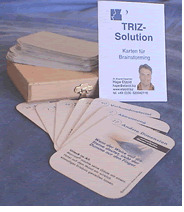
\includegraphics[width=.5\textwidth]{./7.jpg} \\
  ТРИЗ-покер. «Несколько кружек пива, проблема, изобретательность и куча
  гениальных идей. Мозговой штурм будет незабываемым»
\end{center}
Среди покупателей и клиентов -- BASF, DaimlerChrysler, Siemens AG, ALTANA
Pharma, Apcon/itelligence, Reemtsma, Bertelsmann Stiftung. Основные партнеры
по покеру на европейском рынке -- Trisolver, MethoSys, TRIZ Journal, Quality
Engineers. Блестящие отзывы для сайта предоставили Отдел Стратегических Продаж
промышленного гиганта «Siemens» и группа развития новых технологий при
Fraunhofer Institut -- крупнейшем научно-исследовательском институте Германии.
Этот же институт подтверждает экономию с помощью карт 3-дневного
ТРИЗ-семинара.  Можно лишь гадать, о семинарах какого уровня ведут речь
уважаемые ученые.

«Новое платье королевы» шьется споро, но с размахом. Обучающие напитки и
радиопостановки -- лишь вопрос ближайшего будущего. А вот чтобы привлечь
покупателей к новому недорогому методическому пособию по ТРИЗ на
конвенциональном (бумажном) носителе, серьезный издатель -- Академия
Технического Университета города Ульм (TQU Akademie GmbH) -- делает в рекламе
особое ударение на прилагаемую «Таблицу противоречий в формате А2»
\cite{Blaesing2001}. Чему посвящены 70 страниц пособия, предназначенного для
руководителей ТРИЗ-проектов и рабочих групп, несложно догадаться.

В одном из писем, датированном 1985 годом, голос Альтшуллера звучит уверенно и
уже почти снисходительно: «Сейчас 40 приемов имеют лишь историческое значение.
Работаем мы -- в основном -- стандартами» \cite{Altshuller1985}.  К этому
письму, адресат которого, к сожалению, неизвестен, еще не раз придется
обращаться. Шутил Генрих Саулович или заблуждался искренне, но только
историческое значение все больше приобретают стандарты. Вечно живыми оказались
приемы и Таблица.

А в Грац я решил не ехать. Непрофессионально выполненное харакири вполне могут
принять за очередной метод активизации творческого мышления. Начнется
организация учебных семинаров…

\clearpage
\begin{flushright}
  Мудрец не кладет все яйца в одну корзину.\\
  (Мигель Сервантес)
\end{flushright}
\section*{3. Древняя история создания ТВППТП}

\subsection*{Так что будем устранять?}

Причины возникновения и логика развития Таблицы, как механизма выбора
подходящих приемов при устранении технических противоречий, до сих пор,
видимо, не представлялись темами, требующими детального рассмотрения.
«Серьезным инструментам» -- ЗРТС, вепольному анализу или Стандартам --
посвящены многочисленные объемные работы. Таблице же -- сухие строчки в
исторических справках. Во всяком случае, очевидно, что подавляющее большинство
разработчиков и поныне придают истории Таблицы значительно меньшее значение,
чем даже истории возникновения и развития типовых приемов. Между тем, было бы
ошибкой считать, что приемы -- в их современном виде -- являлись первичным, а
Таблица -- вторичным или даже второстепенным продуктом, поскольку именно
появление Таблицы не только легитимировало значительное расширение списка
приемов, но и определило их равноправное (а на некоторых этапах и
доминирующее) положение в структуре ТРИЗ.

Здесь следует напомнить о том, что уже сама предыстория появления приемов и
Таблицы представляется достаточно противоречивой. Впервые идея создания
системы последовательных мыслительных операций, в которой поиски способов
устранения технического противоречия (или его причины) велись бы на основе
исследования типичных приемов (прообразов), была высказана основоположниками
ТРИЗ \textbf{Генрихом Сауловичем Альтшуллером} и \textbf{Рафаилом Борисовичем
  Шапиро}. В опубликованной ими в 1956 году программной статье «О психологии
изобретательского творчества» \cite{Altshuller1956} наряду с использованием
уже известных в природе и различных областях техники прообразов, предлагался и
поиск новых приемов (путем изменения известных прообразов на различных
системных уровнях).

Эту статью часто приводят как некий переломный пункт, обозначивший начало
систематической деятельности \textbf{Альтшуллера} (о \textbf{Шапиро} при этом
как-то забывают) над будущей «изобретательской наукой». При этом собственно
статья имела к психологии лишь поверхностное отношение. Зато материал насыщен
большим количеством примеров технического характера, что должно было создать
впечатление компетентности авторов в раскрываемом вопросе, скрывая скорее
дилетантские познания в области психологии.

Статья оставляет двоякое впечатление: С одной стороны, возникает ощущение, что
авторы стремятся воспользоваться моментом и высказать «наболевшее». Читая
строчки с критикой «советского изобретательства, которое связано с плановым
производством», невольно вспоминаешь о том так и не найденном «письме
Сталину», с которого начались злоключения авторов. Несомненно, они стремились
использовать «временные ресурсы». Ведь статья была написана и опубликована уже
через несколько месяцев после того, как 22 февраля 1956 года -- в ходе XX
съезда КПСС Хрущёв выступил с докладом о разоблачении «культа личности»
Сталина.

С другой стороны, учитывая значительные пробелы в советской специальной
литературе в области изобретательского творчества (как отмечали сами авторы,
«единственная монография по этому вопросу в советской психологической
литературе -- книга П.М. Якобсона «Процесс творческой работы изобретателя» --
была опубликована еще в 1934 г.), нужно было использовать представленную
возможность и «застолбить» те разработки, которые были проведены за предыдущие
годы. Или те, которые хотелось бы провести. Возможно, по этой причине
некоторые темы остались непроработанными, а сама статья не вызвала широкого
читательского резонанса.

Подводя итоги «беглого очерка развития» современного велосипеда, авторы среди
прочего сделали следующие выводы, легшие в основу тезисов первого алгоритма:
\begin{itemize}
\item[3.] Планомерное развитие системы (машины, механизма, процесса)
  оказывается возможным до тех пор, пока не возникнут и не обострятся
  противоречия между более совершенным элементом и отстающими ее частями.
\item[4.] Это противоречие является тормозом общего развития всей системы.
  Устранение возникшего противоречия и есть изобретение.
\item[5.] Коренное изменение одной части системы вызывает необходимость ряда
  функционально обусловленных изменений в других ее частях.
\end{itemize}
Следовательно, каждое творческое решение новой технической задачи --
независимо от того, к какой области техники оно относится, -- включает три
основных момента:
\begin{itemize}
\item[1.] Постановка задачи и определение противоречия, которое мешает решению
  задачи обычными, уже известными технике путями.
\item[2.] Устранение причины противоречия с целью достижения нового -- более
  высокого -- технического эффекта.
\item[3.] Приведение других элементов усовершенствуемой системы в соответствие
  с измененным элементом (системе придается новая форма, соответствующая новой
  сущности)».
\end{itemize}
Практически те же рассуждения были приведены и тремя годами позднее в
следующей совместной статье \cite{Altshuller1959}. Как не трудно заметить,
понятие «изобретение» в смысле «устранение возникшего противоречия» и, как
следствие, «коренное изменение одной части системы» в значительной степени
конфликтует с разработанной соавторами в дальнейшем концепцией ИКР, введенной
уже в АРИЗ-59.  В ней «Идеальный конечный результат -- это ситуация, когда
нужное действие получается без каких-либо затрат (потерь), усложнений и
нежелательных
эффектов»\footnote{\url{http://www.trizland.ru/trizba.php?id=8}}.

Отступая от основной темы, следует все же отметить, что и это -- краеугольное
в ТРИЗ -- понятие Идеального Конечного Результата до сих пор имеет
многочисленные разночтения. Для одних авторов «ИКР -- то чего хотелось бы
добиться в результате решения
задачи»\footnote{\url{http://www.trizminsk.org/e/215104.htm}}. Другим ближе к
сердцу «ИКР -- это наиболее устраивающая нас ситуация, когда требуемое
действие выполняется само, без каких-либо дополнительных усилий и введения в
систему дополнительных
объектов»\footnote{\url{http://www.gnrtr.com/explanations/ru/i01.html}}.
Третьи видят в нем «Идеальное решение, т. е. такое решение, которое не требует
для выполнения необходимого действия введения дополнительных механизмов,
операций технологического процесса. Т. е. действие осуществляется само
собой»\footnote{\url{http://trizway.com/lot-references.php?ref=terms-i}}. Из
всех предлагаемых сегодня формулировок ни одна, тем не менее, не
предусматривает коренные изменения одной из частей системы.

Предложенная в статье \cite{Altshuller1956} двухступенчатая схема «поиска
способа \textbf{устранения причины} технических противоречий» была бы, по
мнению авторов, «наиболее рациональна» и «позволяет получить правильные
решения с минимальной затратой усилий и времени». На тот малоприметный, но
весьма примечательный факт, что в статье упоминаются вперемежку то «приемы
устранения \textbf{причины технических противоречий}», а то «приемы устранения
\textbf{технических противоречий}», как-то не обратили внимания. Судя по
всему, Альтшуллер и Шапиро сами так и не сумели прийти к единому мнению о том,
на какой стадии развития технической системы (в дальнейшем -- ТС) следует
производить ее преобразования с целью получения нового технического
решения. Или не придавали этой детали серьезного значения.

При всей внешней схожести двух формулировок, разница между ними все же есть.
Задача устранения имеющегося (то есть уже возникшего) противоречия,
предполагающая \textbf{дальнейшее улучшение} ТС, ее изменение, преобразование
и т.д., с методической точки зрения значительно отличается от такой постановки
задачи, при которой речь идет об устранении первоначальной причины
противоречия. То есть о таком «устранении», при которой сама ТС останется
неизменной или лишь минимально измененной. Не говоря уже о том, что
«приведение других элементов усовершенствуемой системы в соответствие с
измененным элементом» не только предполагает некоторые затраты (потери),
усложнения и нежелательные эффекты, но и значительно усложняет, а вернее,
отрицает возможность устранения исходной \textbf{причины} технического
противоречия в ее изначальной форме. Хотя бы уже потому, что получившаяся в
результате всех необходимых преобразований ТС (как объект изобретения) нередко
имеет с исходной ТС довольно мало общего.

Неопределенность в целях и задачах будущей системы поиска и выбора приемов
пронизывает всю теоретическую часть статьи. Так в одном месте говорится о том,
что «Оперативная стадия заключается в систематическом и целесообразно
направленном исследовании \textbf{возможных способов устранения обнаруженной
  причины противоречия}». Несколькими абзацами ниже перед нею ставится уже
несколько иная задача: «Работа на оперативной стадии творческого процесса
каждым более или менее опытным изобретателем ведется планомерно. …
Аналитическая стадия творческого процесса во многом упрощает эти поиски:
изобретатель ищет не абстрактную «идею», а конкретные способы устранения
конкретного технического противоречия».

Здесь можно резонно возразить, что в 1956 году еще не было сформулировано
понятие главной полезной функции, как и многие другие элементы ТРИЗ. Дискуссия
на эту тему способна увести от главной темы статьи и значительно более опытных
тризовцев. Очевидно лишь, что далеко не все приводимые в статье рассуждения
строго логичны и взаимосвязаны. Следует отметить и тот факт, что некоторые
высказанные в первой статье идеи, относящиеся к созданию будущего алгоритма,
так и не были включены в его состав. К примеру, важный «Последний этап
творческой работы -- оценка сделанного изобретения» получил свое эксплицитное
выражение лишь через 20 лет в АРИЗ-77 \cite{Altshuller1971}! Логике развития
АРИЗ будет посвящена еще не одна исследовательская работа. Поэтому постараемся
сконцентрироваться здесь лишь на тех его элементах и преобразованиях, которые
имели непосредственное отношение к табулированному применению приемов.

Реализация главной идеи статьи -- схемы «поиска способа устранения причины
технических противоречий» оказалась, судя по всему, делом значительно более
сложным, чем это могло представляться в 1956 году двум еще совсем молодым
людям (тогда им было по 30 лет). Прежде всего, многообразие выявляемых приемов
и явная субъективность не только в их определении, но и в последующем
«узнавании» в новых практических примерах, мешали созданию универсального
прикладного инструмента. Значительная полярность взглядов на дальнейшие пути
развития методики также не давала прийти к согласию. И, скорее всего, не
случайно первые решительные попытки табуляции созданных групп (списков)
приемов и последующего создания Таблицы технических противоречий произошли
лишь после того, как Шапиро прекратил свою работу в ТРИЗ. С одной стороны, это
значительно ослабило позицию Альтшуллера -- как ослабляли его всякий раз
«уходы» соратников и учеников, с другой -- развязало ему руки. Если в вопросе
создания АРИЗ и разработке абстрактных шагов мысленного эксперимента
соавторство не только допускалось, но даже приветствовалось, то гораздо более
субъективные приемы и будущая Таблица терпели лишь одного автора.

Но возможно, что причину раскола следует искать в несхожести взглядов на
реализацию самой оперативной стадии. Как уже отмечалось, в трактовках
оперативной стадии кроется явное противоречие, как если бы авторы, не сойдясь
во мнениях, писали эту статью по очереди. При всей неоднозначности основной
функции, которую Альтшуллер при поддержке Шапиро возлагал на Оперативную
стадию, явно угадывается стремление авторов отвести механизму выбора
подходящего приема, выводящего на «правильное решение», ведущую роль в будущем
алгоритме. Не исключено, что уже тогда развернулась дискуссия о возможности в
будущем заменить оперативную стадию, свернув ее в компактный и универсальный
механизм. Можно предположить, что Шапиро придерживался более «романтической»
точки зрения и настаивал на «систематическом и целесообразно направленном
\textbf{исследовании возможных способов}». В то время, как более конкретный и
постоянно нацеленный на конечный результат Альтшуллер видел будущее методики в
создании системы стандартных (типовых) и одинаковых -- \textbf{конкретных} --
для всех пользователей способов (приемов) устранения конкретного технического
противоречия.

\subsection*{Рожденная НТР?}

В связи со всем вышеизложенным не может не представлять интерес другой вопрос:
А было ли появление в ТРИЗ такого инструмента, как Таблица, неизбежным
эволюционным шагом в развитии будущей изобретательской науки и
непредотвратимым явлением, порождением объективных закономерностей? Или
рождение Таблицы было вызвано искусственно, а дальнейшее развитие подчинялось
требованиям далеко не всегда объективных внешних обстоятельств? Ответ на эти
вопросы представляется далеко не простым. Зарождение Таблицы, как и
неудавшаяся десятилетием позже попытка «отстранения ее от дел» отражают,
возможно, непростые личностные взаимоотношения, субъективные и зачастую
полярные взгляды участников этого процесса на различных его этапах.

Большинство европейских любителей ТРИЗ искренне уверены в том, что Таблица
была создана сразу в ее «классическом» варианте, сочетающем 39 характеристик и
использующем 40 приемов. Что это первый и последний, единственный и неизменный
путеводитель по загадочной, завораживающей внимание и возбуждающей фантазию
Стране Изобретательских Приемов. Впрочем, заблуждение это разделяют не только
начинающие любители ТРИЗ. 
\begin{quote}
  Разработка понятия «Противоречие» привела к появлению понимания противоречий
  как типовых задач, предполагающих типовое же решение. Из них и шагов
  Оперативной стадии в 1963 г. возникли «Типовые приёмы разрешения технических
  противоречий», годом позже сведённые в широко известную таблицу. Поначалу
  их было 40, затем появились ещё 10 [П5]. Сама таблица с 1971 г. уже не
  менялась. \cite{Korolyev1998}
\end{quote}
Мнение автора статьи, помещенной в «Энциклопедии ТРИЗ» в значительной степени
отражает современный подход к формированию знаний о создании Таблицы, как и
энциклопедических знаний о ТРИЗ в целом. Тем не менее, приведенную цитату
следовало бы помещать в сертификационном билете на 2-й уровень с заданием
«Найдите в тексте три ошибки». В действительности, приемов было поначалу не
сорок.  И «широко известной» Таблица 1964 года по разным причинам так и не
стала.  А не менялась Таблица после 1971 года только самим Альтшуллером (по
причинам, упомянутым в первой статье).

Любопытным представляется упомянутое разъяснение: 
\begin{quote}
  П5. Позднее появилось уточнение: «Типовые приёмы разрешения
  \textbf{характеристических} технических противоречий». То есть,
  противоречий, привязанных к определённому набору конкретных характеристик
  технических систем, аналогичных \textbf{характеристическим} уравнениям
  математического анализа.
\end{quote}
Но, поскольку поисковая машина Фонда Г.С Альтшуллера пока ни одной статьи со
словом «характеристических» не находит, а ссылок в Интернете, кроме как на
саму статью в «Энциклопедии ТРИЗ», тоже больше нет, следует пока что отнести и
эту информацию к разряду NT («утка», непроверенно).

\begin{center}
  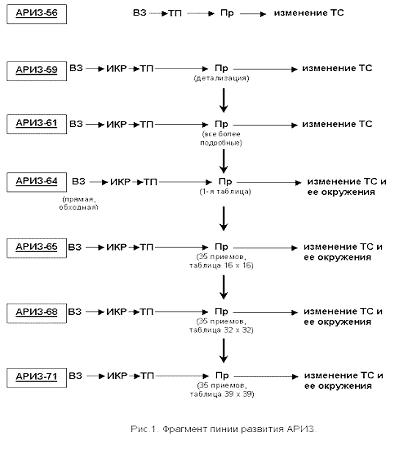
\includegraphics[width=.7\textwidth]{./8.jpg}
\end{center}

Ю.П. Саламатов \cite{Salamatov1992} также считал, что Таблица появилась уже в
АРИЗ-64. В составленной им линии развития АРИЗ она упоминается в составе
АРИЗ-64 как «1-я таблица» из четырех, правда, без указания числа приемов
(Рис. 1).

Но в АРИЗ-64, опубликованном Официальным Фондом Г.С. Альтшуллера (выдержка из
книги \cite{Altshuller1964}), работа с Таблицей технических противоречий, как
составляющая часть шагов оперативной стадии, не упоминается.  Да и в конспекте
«История развития АРИЗ» \cite{Altshuller1986a}, говоря об АРИЗ-64, Альтшуллер
упоминает о ней, скорее, мимоходом: «\textbf{Впервые} составлена таблица
\textbf{групп приемов}».  Он даже не считает ее \textbf{первой} Таблицей, --
\textbf{первая} появляется, по его мнению, лишь в АРИЗ-65.

Можно лишь предположить, что последователи Генриха Сауловича «обобществили»
АРИЗ-64 с материалами его книги, в которой эта версия алгоритма была изложена.
Ведь даже понятие технического противоречия в АРИЗ-64 встречается лишь однажды
-- в первом шаге оперативной стадии: «Проверить возможность устранения
технического противоречия изменением данного объекта (машины, механизма,
процесса)».  Таблицы же в нем нет и в помине.

Группа специалистов из ТРИЗЛАБ (Ideation TRIZLAB of the International TRIZ
Association), в составе которой сразу три Мастера ТРИЗ, «свернула» историю
создания Таблицы радикально: «Таблица и приемы были созданы в 1971 году и
явились одним из первых эффективных инструментов
ТРИЗ»\footnote{\url{http://www.trizscientific.com/TRIZ_sci/history/history09_recomend_r.htm}
  -- no more online. HGG}.  При этом отмечены основные заслуги автора:
«Альтшуллер внес двойной вклад в развитие рекомендаций для изобретателя:
\begin{itemize}
\item Основал рекомендации (приемы) не на субъективном опыте изобретателей, а
  на анализе патентного фонда (к уровню объективности этой процедуры нам еще
  предстоит вернуться -- Л.Ш.).
\item Перешел от одномерной структуры предъявления приемов (список) к
  двухмерной (таблица технических противоречий), позволяющей более эффективно
  отыскивать нужные рекомендации.
\end{itemize}
Столь же браво обошлись Мастера ТРИЗ-Лаб и с историей
АРИЗ\footnote{\url{http://www.trizscientific.com/TRIZ_sci/history/history06_ariz_r.htm}
  -- no more online. HGG}.  Явное противоречие в указаниях даты рождения
Таблицы, размещенных на соседних страницах сайта, их, по-видимому, ничуть не
смутило:
\begin{quote}  
  1959 Первый вариант краткого алгоритма (без названия «алгоритм) в первой
  опубликованной статье по ТРИЗ

  1960 \textbf{Появление названия «Алгоритм изобретения»} и 5 шагового
  циклического алгоритма

  1964 ARIZ-64

  1969 \textbf{ARIZ-69 с таблицей приемов разрешения технических противоречий} 

  1971 ARIZ-71 с физическим противоречием
\end{quote}
Сравним выделенные строки с конспектом Г.С.Альтшуллера «История развития
АРИЗ» \cite{Altshuller1986a}:
\begin{quote}  
  АРИЗ-65. \textbf{Введена первая (еще очень небольшая) таблица устранения
    технических противоречий}. Оперативная часть по-прежнему включает анализ
  природных прототипов. \textbf{Впервые появилось слово «алгоритм»} -- как
  указание на дальнюю цель развития программы».
\end{quote}
Итак, по мнению Альтшуллера, первая Таблица была введена в АРИЗ-65. Что же
было до нее? Становится очевидным, что «История развития АРИЗ» (и Таблицы как
одной из его составляющих) далеко не так однозначна, как кажется. И
разобраться в ней -- дело не такое уж простое.

На сайте ТРИЗ-Лаб говорится и о том, что еще в конце 80-х года было
предпринято «несколько неудачных попыток разработки новых версий ARIZ --
Королева, Андриевского, Ладошкина и других. Г. Альтшуллер возражал против
того, чтобы кто-то кроме него разрабатывал версии АРИЗ, так как АРИЗ является
его авторским
материалом»\footnote{\url{http://www.trizscientific.com/TRIZ_sci/history/history06_ariz_r.htm}
  -- no more onlien. HGG}.  Но прошло несколько лет, и «в 1989 Альтшуллер
официально разрешил разработку «не альтшуллеровских» версий алгоритма. Тогда
же состоялось совещание с участием Зусман, Злотина, Злотиной, Литвина, Петрова
по разработке новой версии ARIZ».

Противоречивые и (как в дальнейшем нетрудно будет заметить) зачастую неверные
версии «Новой истории ТРИЗ» не только мешают постичь логику развития методики
и ее основного логического механизма -- АРИЗ, но и ее «главного» (по частоте
применения) на сегодняшний день инструмента -- Таблицы. Учитывая уже
упоминавшиеся в первой статье особенности формирования авторского коллектива
на начальных стадиях, они лишают нас возможности понять и оценить вклад того
или иного соавтора в развитие АРИЗ и его частей. Интересно понять, что же
происходило на самом деле, как складывалась «история развития ТРИЗ».
Реализуемо ли это при таком значительном различии мнений?

Ответ на этот вопрос предложил сам Г.С. Альтшуллер. В перечне ходов ЖСТЛ
\cite{Altshuller1994} в разделе Постэндшпиль дается недвусмысленная
рекомендация (№ 84) реакции на ход внешних обстоятельств. «Искажение истории»:
Ход творческой личности -- «Использование архивного материала». В целях
постепенного и неуклонного формирования в себе качеств творческой личности,
будем стараться максимально использовать открытые публикации, доступные
архивные материалы и свидетельства.

Общее число рабочих вариантов Таблицы достоверно не известно. Выборочный опрос
Мастеров ТРИЗ показал, что таковых могло быть от одного до четырех. Впрочем,
мало (очень-очень мало) кто из Мастеров готов перечислить даже три варианта.
Так что этот вопрос вполне можно использовать на экзаменах в качестве
«завального». Впрочем, это и не удивительно. Несмотря на самоотверженную
работу Фонда ГСА по опубликованию работ и ЧОУНБЭ -- по их сбору, классификации
и предоставлению рабочих материалов, в общедоступном виде (например, в
Интернете) находятся, действительно, лишь два-три варианта. На первый взгляд,
может показаться несущественным то значение, которое придается здесь времени
включения Таблицы в АРИЗ. В действительности, с учетом дополнительных
сведений, почерпнутых из «второстепенных» источников, это обстоятельство имеет
особый, и, как будет показано в дальнейшем, важный смысл.

«Раскопки» в архивах, проведенные при подготовке этой статьи, показали, что за
относительно короткий период своего роста и преобразования Таблица имела не
менее шести разновидностей, пять из которых опубликованы. И лишь три варианта
включались самим Альтшуллером в качестве составных частей в Алгоритмы Решения
Изобретательских Задач: АРИЗ-65 (16 параметров / 35 приемов), АРИЗ-68 (32/35)
и АРИЗ-71 (39/40). Возможно, что некоторые «зародышевые» и промежуточные
варианты просто затерялись или забылись в повседневной борьбе за продвижение
основных идей ТРИЗ. Все же представляется важным выделить в них хотя бы
основные отличия, позволяющие проследить логику развития и видоизменения этого
главного инструмента тризного зарубежья.

\subsection*{Ты помнишь, как все начиналось?}

В 1992 году Ю.П. Саламатов отметил, что «в ТРИЗ осталось множество белых
пятен, неисследованных и недостаточно понятых проблем и разделов»
\cite{Salamatov1992}. Возможно, он и не был первым, кто это заметил. Но он был
первым, кто сделал это мастерски. Освещая в своей работе «самые серьезные
исследования по ИМ-ТРИЗ-технологии», Саламатов сделал особое ударение на том,
что «в ходе этих работ идет интенсивная проверка степени разработанности,
истинности, зрелости всех разделов ТРИЗ -- базы знаний новых компьютерных
систем. Вскрываются новые пласты теории, по-новому представляются некоторые
разделы, четко проявляются недостатки, недоработки, становятся видными
перспективы развития теории изобретательства». \textbf{Разработанность,
  истинность, зрелость!} -- Здорово сказано!  Красиво.

Но, отслеживая вехи становления и преобразования «железной леди», так и тянет
спросить: «А кто же все-таки помнит, как все начиналось?» Но спросить не у
кого. Вот о том, как возникали стандарты, можно спросить у Мастера ТРИЗ
В. Петрова. О «диверсионке» -- у Мастера ТРИЗ Б. Злотина. О справочнике
физэффектов у Мастера ТРИЗ Ю. Горина. Об АРИЗ когда-то можно было спросить у
Кандидата в Мастера ТРИЗ Р. Шапиро. А про ЭТО?

На соавторство или хотя бы на сопереживание в создании Таблицы, похоже, никто
и никогда всерьез не претендовал. Ею от начала и до конца занимался только
Альтшуллер, и именно \textbf{его} последний вариант, ценит и безоговорочно
принимаемый всем тризным и околотризным миром, канонизирован и причислен к
лику святых. В чем секрет этого признания? В том ли, что в Таблице все так
фантастически просто? Или в том, что история ее создания, как и стоящая за нею
технология, практически никому неизвестны? Элементарность ли заполняющих
Таблицу счастливых номеров завораживают новичков ТРИЗ, или непостижимая даже
для самого смелого воображения необозримость океана переработанной информации,
словно гипнотизируя, заставляет даже видавших виды Мастеров вновь и вновь
полагаться на удачу в ТРИЗном Лото?

В опубликованной в 1961 году в книге «Как научиться изобретать»
\cite{Altshuller1961} АРИЗ-61 («улучшенная модификация АРИЗ-59«) новые
разработки уживались со старыми проблемами. «Расширена оперативная часть. Но
правил выполнения шагов по-прежнему нет» \cite{Altshuller1986a}. Расширение
произошло за счет развертывания уже имевшихся трех шагов и введения четвертой
группы -- списка из четырех приемов, проверяющих возможности разделения
объекта на независимые части. Именно эти четыре группы, включающие 20 приемов,
были условно сведены в тексте книги в первую, пока еще виртуальную таблицу
будущего: «Изобретателю полезно иметь таблицу таких приемов и постоянно ее
пополнять, приглядываясь к методам решения различных технических задач. В
качестве основы для таблицы могут послужить четыре группы приемов, с которыми
мы уже познакомились. При пополнении таблицы \textbf{можно не заботиться о
  строгости классификации. Достаточно, чтобы приемы располагались от простого
  к более сложным}. Когда техническое противоречие выявлено, изобретатель
должен, не полагаясь на память, взять лист с таблицей приемов и
последовательно проверить пригодность каждого приема. Проверить без спешки, не
отдавая заранее предпочтения тому или иному приему, не пропуская приемы,
кажущиеся «заведомо непригодными». Очень часто лучшее решение дают именно эти
заведомо непригодные приемы».

Поскольку «улучшение» в АРИЗ-61 по сравнению с АРИЗ-59 носило пока еще
значительно более выраженный количественный, чем качественный характер (хотя
будущий переход количества в качество и наметился), авторами этой
«модификации», по-прежнему следовало бы считать дуэт Альтшуллер-Шапиро. Ведь,
как уже отмечалось, «Шапиро проработал в ТРИЗ по 1961-й год». Ну, добавилась
еще одна группа? Ну, появились еще четыре приема? По сути-то обе модификации
идентичны. Правда, немного смущают даты. Было ли расширение оперативной части
и распад дуэта в 1961 году простым совпадением? Проработал Шапиро «в ТРИЗ» по
1961-й год -- только до появления новой группы приемов, или он ушел уже после
этого?

В 1961 году была издана книга Шапиро \cite{Bachmatov1961}. Судя по тому, что и
книга Альтшуллера была издана в том же году, а ее подготовка и написание
заняли, возможно, не один месяц, отход Шапиро от совместной работы произошел
уже после или во время введения в АРИЗ новой группы приемов. Могло ли иметь
столь малозначительное, на первый взгляд, расширение оперативной стадии АРИЗ
какое-то отношение к его решению? А может быть, четвертая группа приемов
именно потому и смогла войти в АРИЗ-61, что Шапиро уже не хотел или не был в
состоянии этому помешать? Ведь он был единственным, кто мог противиться
механистическому расширению АРИЗ.

Ответы на эти и многие другие вопросы, возможно, будут найдены в личных
архивах основоположников ТРИЗ, в их переписке, набросках и черновиках.
Остается надеяться, что тризное движение достигнет в обозримом будущем такого
размаха, при котором подобные «раскопки» начнут представлять интерес и для
широкой общественности.

Сравнительный анализ ранних вариантов алгоритма показывает, что в них
«табличные» свойства присущи группам приемов лишь в зачаточном состоянии
(1.-4. шаги оперативной стадии) -- к преобразованию в какой-либо механизм,
например, сведению в Таблицу, они еще совершенно не были готовы. Причин тому
видится несколько. В первую очередь, это отсутствие правил выполнения шагов в
целом и чересчур общее, абстрактное определение части из них (в особенности, в
составе третьего и четвертого шагов).

Вот эти группы, без особых ухищрений представленные в виде шагов оперативной
стадии АРИЗ-61:

\textbf{Первый шаг.} Проверка возможных изменений в самом объекте (т. е. в
данной машине, данном технологическом процессе).
\begin{itemize}
\item[1.] Изменение размеров.
\item[2.] Изменение формы.
\item[3.] Изменение материала.
\item[4.] Изменение температуры.
\item[5.] Изменение давления.
\item[6.] Изменение скорости.
\item[7.] Изменение окраски.
\item[8.] Изменение взаимного расположения частей.
\item[9.] Изменение режима работы частей с целью максимальной их нагрузки.
\end{itemize}
\textbf{Второй шаг.} Проверка возможности разделения объекта на независимые
части.
\begin{itemize}
\item[1.] Выделение «слабой» части.
\item[2.] Выделение «необходимой и достаточной» части.
\item[3.] Разделение объекта на одинаковые части.
\item[4.] Разделение объекта на разные по функции части.
\end{itemize}
\textbf{Третий шаг.} Проверка возможных изменений во внешней (для данного
объекта) среде.
\begin{itemize}
\item[1.] Изменение параметров среды.
\item[2.] Замена среды.
\item[3.] Разделение среды на несколько частичных сред.
\item[4.] Использование внешней среды для выполнения полезных функций.
\end{itemize}
\textbf{Четвертый шаг.} Проверка возможных изменений в соседних
(т.е. работающих совместно с данным) объектах.
\begin{itemize}
\item[1.] Установление взаимосвязи между ранее независимыми объектами,
  участвующими в выполнении одной работы.
\item[2.] Устранение одного объекта за счет передачи его функций другому
  объекту.
\item[3.] Увеличение числа объектов, одновременно действующих на ограниченной
  площади, за счет использования свободной обратной стороны этой площади.
\end{itemize}

Несмотря на расширение, оперативная стадия АРИЗ-61 все еще мало чем отличалась
от классического списка контрольных вопросов. Как и в АРИЗ-56, а затем и в
АРИЗ-59, «Оперативная часть сходна с синектикой -- расчет на аналогию (прежде
всего -- на использование природных прототипов)» \cite{Altshuller1986a}.
Введение «разделительных» приемов, действительно отличающихся технической
новизной, лишь указало на возможности дальнейшего увеличения списка, но вовсе
не сделало «третью по счёту версию гораздо «алгоритмичней«», как это пытается
представить автор будущей Энциклопедии ТРИЗ \cite{Korolyev1998}.

Правило распределения приемов в будущей Таблице (и, следовательно, порядок их
применения), сводящееся к их расположению «от простого к более сложным» должно
было увеличивать эффективность перебора вариантов, повышая вероятность
нахождения удачного приема еще до завершения полного просмотра всех групп. Но
перебор вариантов как таковой (а, следовательно, и МПиО в целом) это решение
еще вовсе не исключало. Возможно, именно неразработанность механизма
применения приемов, их бросающаяся в глаза неалгоритмичность служили причиной
того, что приемам еще не придавалось первостепенного значения в развитии АРИЗ.
Во всяком случае, имелись серьезные затруднения в определении этого значения.
А ведь именно на приемах и «прообразах» была выстроена практически вся
оперативная стадия (см. приведенный выше фрагмент АРИЗ-61) и, как следствие,
именно на них ложилась основная ответственность за успешное применение АРИЗ.
Эти обстоятельства и вынуждали Альтшуллера производить регулярную перепись
приемов, чтобы нащупать в них скрытые закономерности и попытаться их
«приручить». Прежде всего, это требовалось затем, чтобы «развернув» шаги
оперативной стадии, вывести приемы -- хотя бы визуально -- из опасной зоны
действия МПиО.

Появление собственно развернутых групп (списков) приемов фактически произошло
уже в АРИЗ-59 -- в первых трех шагах оперативной стадии (ОС), только здесь они
еще не были пронумерованы. Альтшуллер и Шапиро отказались от термина «прием»
при поиске решений в системе, надсистемах и внешней среде (подшаги второго
шага, перенесенные в начало оперативной стадии), заменив его на «возможные
изменения». А «типичные приемы (прообразы)» решения в природе и технике были
окончательно переименованы в «прообразы» и, таким образом, формально лишены
статуса «приемов». В АРИЗ-61 произошло лишь одно принципиальное изменение --
добавление во втором шаге ОС четвертой (с учетом «прообразов» -- шестой)
группы специальных приемов, узко направленных на «проверку возможности
разделения объекта на независимые части».

Те же пять групп приемов, составлявшие оперативную стадию (в неразвернутом,
тезисном виде), присутствовали и в самом первом пра-алгоритме -- АРИЗ-56
\cite{Altshuller1956}:
\begin{itemize}
\item[1.] Исследование типичных приемов решения (прообразов):
  \begin{itemize}
  \item[а)] в природе,
  \item[б)] в технике.
  \end{itemize}
\item[2.] Поиски новых приемов решения путем изменений:
  \begin{itemize}
  \item[а)] в пределах системы,
  \item[б)] во внешней среде,
  \item[в)] в сопредельных системах.
  \end{itemize}
\end{itemize}
Оперативная стадия АРИЗ-59 отличалась от предложенного в статье 1956 перечня
шагов лишь некоторой их детализацией. Кроме того, изменилась
последовательность шагов: «Поиски новых приемов путем изменений» переместились
на первое место, сдвинув «Исследование типичных приемов решения (прообразов)»
в конец стадии. Зато в АРИЗ-61 году произошел своеобразный прорыв в развитии
структуры оперативной стадии. Введение на втором шаге пока еще небольшой
группы новых приемов на «выделение части» и «разделение на части» открывало
новые перспективы для расширения до тех пор еще обозримого списка подшагов.
Перечень «изменяющих приемов» не просто увеличился на 4 пункта, но
«развернулся» и был значительно детализирован, приняв форму списка проверочных
рекомендаций из 20 отдельных приемов. В большинстве своем (первый и второй
шаги) эти приемы носили уже вполне прикладной характер, который еще нагляднее
подчеркивался новыми приемами:
\begin{quote}
  Второй шаг. Проверка возможности разделения объекта на независимые части.
  \begin{itemize}
  \item[1.] Выделение «слабой» части.
  \item[2.] Выделение «необходимой и достаточной» части.
  \item[3.] Разделение объекта на одинаковые части.
  \item[4.] Разделение объекта на разные по функции части.
  \end{itemize}
\end{quote}

Все 20 приемов в АРИЗ-59 по-прежнему носили общий, универсальный и
ненаправленный характер, как по отношению к будущему решению, так и по
отношению к исходной изобретательской ситуации. Это обстоятельство и вынуждало
применять их при поиске решения, как и в 1956-м, «в последовательности от
простого к сложному, что позволяло получить правильные решения с минимальной
затратой усилий и времени». Рекомендации авторов были фактически излишни,
отражая лишь объективную слабость приемов и неизбежную необходимость их
перебора. Применение приемов в очередности, соответствующей убыванию их
простоты и частоты употребления, обещало, на первый взгляд, некоторое
повышения вероятности нахождения «правильного решения» еще до окончания всего
списка.

Однако с ростом числа приемов все более заметно стало обостряться новое
противоречие. Как не раз отмечалось, «Сами приемы не несут в себе конкретных
решений. Увидеть решение, развернуть его на основе предлагаемого принципа или
подсказки должен сам решающий задачу. Поэтому работа с каждым приемом не может
быть простой и быстрой. На прием надо настроиться, внимательно и скрупулезно
просмотреть возможности использования заложенных в нем рекомендаций под самыми
разными углами зрения. Даже в самом экономном, ускоренном режиме работа с
одним приемом занимает в процессе реального решения задач не менее
получаса». \cite{Kudryavtsev}

Иными словами, регулярное применение 16 приемов в 1959 году занимало в
процессе решения задачи от 4 до 8 часов интенсивной групповой или
индивидуальной работы. Введение же четвертой группы приемов, определившее
новое направление развития АРИЗ, ставило их комплексное применение под угрозу
невыполнимости. Непомерные затраты времени на перебор уже имевшихся приемов
воздвигали мощный барьер перед соблазнительной перспективой дальнейшего
расширения списка. Но самой значительной проблемой по-прежнему оставалось их
ненаправленное применение.

Используя столь любимую Альтшуллером практику аналогий, применение приемов
можно было представить как стрельбу из лука по кучевым облакам
изобретательской ситуации, возможно, содержащим в себе нужные идеи для
«правильного решения». Стрелами являлись приемы -- каждый со своим порядковым
номером и определенными свойствами. «Правильное решение», как предполагалось,
крылось где-то в облаке изобретательской ситуации. Решателю предлагалось
поупражняться в стрельбе из лука, стараясь попасть в его невидимый центр -- в
надежде вызвать выпадение благодатного «дождя» идей, устраняющего противоречие
на пути к ИКР (Рис. 2).

\begin{center}
  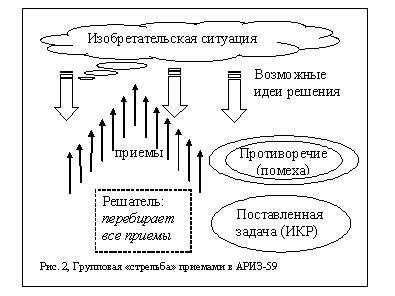
\includegraphics[width=.7\textwidth]{./9.jpg}
\end{center}

При этом не было ясно, откуда нужно стрелять и какое направление выбирать.
Занять ли для стрельбы постоянную позицию или передвигаться от выстрела к
выстрелу, но куда? Стрелять в центр облака или в самое «темное» его место?
Ясно было лишь одно: Желательно воспользоваться всеми стрелами по очереди.
Поэтому все стрелы-приемы запускались (каждым решателем в отдельности) из
одной точки и летели в одном и том же направлении (а порой и в одно место): От
решателя, с его субъективным видением приемов, прямо в «облако»
изобретательской ситуации.

Как следствие, получение одной из возможных идей решения поставленной задачи
(идеального результата) являлось скорее функцией удачливости и опыта,
накопленного решателем, чем объективной силы предлагаемых приемов. Неизбежно
возникала парадоксальная ситуация, при которой объективно полезное сужение
постановки задачи приводило к снижению вероятности результативного попадания
каждым из приемов (использование которых оставалось, несмотря на имеющиеся
примеры, делом крайне субъективным) в отдельности. В особенно невыгодное
положение ставило это обстоятельство начинающих решателей.

Необходимость перебора всех вариантов, ненаправленность действия приемов,
субъективность выбора последовательности их применения, снижение вероятности
результативного попадания в результате сужения постановки задачи -- все это
снижало привлекательность работы на оперативной стадии, так же как и
эффективность алгоритма в целом. Нестабильность на оперативном участке АРИЗ
неизбежно отражалась и недоверием к его работоспособности, причем не только у
новичков. Первой попыткой конструктивного решения этих проблем стало
объединение в 1964 году накопленных приемов в «таблицу групп приемов», которую
Альтшуллер подробно описал в своей новой книге «Основы изобретательства»
\cite{Altshuller1964}, но не решился официально включить в состав алгоритма.
\clearpage

\begin{flushright}
  «Чтоб музыкантом быть, так надобно уменье…«\\
  (И.А. Крылов, Квартет)
\end{flushright}
\section*{4. Впервые составленная таблица групп приемов}

Как уже отмечалось, внешний вид, форма и структура Таблицы на разных этапах ее
становления не только соответствовали ее реальному внутреннему содержанию,
объемам и качеству переработанной при ее подготовке информации или
возможностям практического применения, но и отражали развитие представлений
авторов о ее функциях. Вернее, автора. Ведь Таблица (то есть собственно
числовая матрица) является уникальным явлением и, возможно, единственным
атрибутом ТРИЗ, по отношению к которому допустимо было утверждать -- по
крайней мере, до сих пор, -- что идея его создания, его разработка,
преобразования и отладка принадлежат Альтшуллеру, только Альтшуллеру и никому
другому.

Следовательно, допустимо было бы также предположить, что именно на примере
Таблицы и связанным с нею изменениям в АРИЗ последователям Генриха Сауловича
предоставляется редкая возможность проследить изменение его представлений о
ТРИЗ на значительном отрезке времени.

В изданной в 1961 году первой книге Г.С. Альтшуллера «Как научиться
изобретать» \cite{Altshuller1961} Таблицы как таковой мы не находим.
Следовательно, допустимо утверждать, что в 1961 году ее еще не существовало.
Зато приемам и их применению отведено немало места в главах, посвященных
примерам разбора задач по АРИЗ: «Поиски ведутся по определенной рациональной
системе. Общей формулы нет, но есть приемы, достаточные для большинства
случаев. Изобретателю нужно систематически перепробовать эти приемы. Как
правило, один из них дает искомое решение».

Очевидно, что только весьма ограниченное число приемов позволяло автору
рекомендовать решателям фактически Метод Проб и Ошибок, чтобы «систематически
перепробовать эти приемы». «Максимум нового эффекта при минимуме затрат на
реализацию -- такова формула хорошего изобретения», -- этот призыв Альтшуллера
в не меньшей степени относился и к самому творческому процессу. Минимум затрат
на поиск нужного приема при максимально успешном результате, -- так можно было
бы сформулировать новую стратегическую цель развития ТРИЗ на ближайшие годы.

Первой (во всяком случае, первой официально зарегистрированной в работах
Г.С. Альтшуллера) попыткой конструктивного решения проблем, связанных с
использованием приемов, стало их объединение в 1964 году в «таблицу групп
приемов». Альтшуллер подробно описал эту таблицу в своей второй книге «Основы
изобретательства» \cite{Altshuller1964}, но из-за обстоятельств, остающихся
пока еще малопонятными, не стал включать в состав алгоритма.

\subsection*{Не выплеснуть ребенка с грязной водой…}

Насколько тернистым и нескорым мог быть путь к новой идее, можно представить,
вспомнив высказывание Альтшуллера: «Когда техническое противоречие выявлено,
изобретатель должен, не полагаясь на память, взять лист с таблицей приемов и
последовательно проверить пригодность каждого приема. Проверить без спешки, не
отдавая заранее предпочтения тому или иному приему, не пропуская приемы,
кажущиеся «заведомо непригодными». Очень часто лучшее решение дают именно эти
заведомо непригодные приемы» \cite{Altshuller1961}.

Конечно, в 1961 число приемов было еще невелико. И таблице, описанной в книге,
пока еще не отводилась роль панацеи в деле устранения технических
противоречий. Ее задачей было лишь немного упорядочить их применение, «не
заботясь о строгости классификации». Собственно, и таблицей предлагаемый
список можно было называть лишь условно -- по признаку делимости приемов на
тематические группы.

«Достаточно, чтобы приемы располагались от простого к более сложным»,
утверждал автор. На вопрос о том, что именно подразумевалось под простотой или
сложностью приемов, читатель не получал однозначного ответа. Но, судя по тем
примерам, которыми были снабжены отдельные приемы, можно было сделать
определенные предположения. «Простыми» следовало считать приемы, более или
менее стабильно и быстро узнаваемые самим автором в новых технических решениях
и задачах.

Возможно, не отдавая себе отчета в важности сделанного заявления, Альтшуллер
отверг саму возможность создания реального механизма, способного обеспечить
объективный выбор наиболее подходящих приемов. Ведь чем точнее и изощреннее
был бы этот инструмент, чем больше «заведомо непригодных» приемов удавалось бы
отсеять с его помощью уже на подготовительной стадии работы, тем выше
становилась бы вероятность потери «лучших решений».

Да уж. Такому противоречию не были бы рады и опытные тризовцы наших дней. Но…
Альтшуллер или не заметил его остроты, или сделал вид, что не заметил. Так или
иначе, он интенсивно разрабатывал, разыскивал, придумывал и заимствовал все
новые и новые приемы. Мысль о том, что таким образом он увеличивает и число
«заведомо непригодных» приемов, отсеять которые с каждым расширением списка
становится все труднее и рискованнее, Генриха Сауловича пока еще всерьез не
тревожила.

ТРИЗ проскочила исторический разъезд на полном ходу, и машинист не заметил,
что путевая стрелка направила его в тупик. Эффективный механизм выбора
«правильных приемов», как идеальная, но недостижима цель, остался где-то в
стороне.

Оглядываться на расставляемые собственными руками логические капканы и ловушки
было некогда: АРИЗ «расширялся», Альтшуллер экспериментировал, зарождались
новые, давно уже «назревшие» инструменты, наглядно свидетельствующие о
планомерном развитии всей методики. Новой оригинальной разработке суждено
обернуться действенным инструментом, позволяющим АРИЗ оправдать и свое
название, и высокое предназначение.

\subsection*{Лирическое отступление}

В предыдущей статье отмечалось, что одной из причин низкой эффективности при
использовании приемов была низкая «прицельность стрельбы». Уровень
объективности использования приемов определялся и оценивался самим решателем.
Отсутствовала определенность при выборе исходной позиции. Неопределенность в
работе с приемами осложняла восприятие решателем логики оперативной стадии,
тормозила развитие АРИЗ и всей методики в целом.

Но, в первую очередь, «страдали» сами приемы.

Этот эффект знаком любому преподавателю, хоть раз включавшему Таблицу в
программу своих семинаров. За первыми восторгами от успешного применения
приемов при решении учебных задач следуют уже менее убедительные подходы
преподавателя к решению производственных задач слушателей. А затем наступает
неизбежная развязка. После нескольких попыток самостоятельного использования
табличного инструментария на практике, доверие к нему у большинства слушателей
семинаров заметно снижается. Ни блестящая эрудиция лектора, ни эффектные и
убедительные примеры зачастую не могут преодолеть той беспомощности, которую
испытывают начинающие тризовцы, оставаясь один на один с реальной задачей.

В том, что вот уже третье поколение преподавателей ТРИЗ великолепно, быстро и
безошибочно -- да что уж скромничать, просто блестяще решает \textbf{Учебные
  Задачи}, заслуга в значительной степени «основоположников» методики. Большая
часть решений таких задач, ставших классикой ТРИЗ, -- это значительно
упрощенные, на первый взгляд методические разборы их поэтапного решения,
ретроспективно «притянутые за уши» к нескольким блестящим идеям. Ни
всеобъемлющего описания проблемной ситуации, ни заблуждений и уводящих в
сторону заманчивых линий развития, которые неизбежно присутствуют в каждом
реальном проекте, ни строгой логики в анализе результата учащиеся в этих
примерах, как правило, не находят.

Поиск решений, которых во всякой реальной ситуации (в отличие от «учебной«)
всегда несоизмеримо больше, неизбежно ведется на многоуровневой основе. При
этом использование приемов, если такое вообще допустимо, способно как-то
оживить этот поиск только для простейших минимальных задач развития, до
которых ой как не просто докопаться. Тому, кто на это способен, приемы
становятся практически не нужны.

Сказать об этом компетентно смогли бы сегодня, в лучшем случае, два-три
десятка решателей. Но в открытую поднимать эту тему считается неприличным.
Абсолютно честного, подробного и полного «конспекта» серьезного ТРИЗ-проекта,
начинающегося с постановки задачи заказчиком и заканчивающегося внедрением
полученной концепции решений в производство, встречать пока еще не
приходилось. А свернутый в десяток страниц успешный «экспресс»-анализ способен
убедить только новичков или профанов.

Немудрено, что большинство тризовцев, долгое время специализирующихся на
преподавании основ методики, привносят в свою будущую практическую
деятельность элементы шапкозакидательства. Мол, сейчас «вколем» пару
приемчиков -- и все пройдет.

Особенно ярко проявляется эта тенденция у «новых тризовцев» на Западе, где
роль упаковки при продаже любого товара давно уже играет существенную, если не
определяющую роль. А истоки такого наполеоновского отношения к любым проблемам
лежат «у колыбели» ТРИЗ. Ведь сам «методический подход» начался с выделения
«готовых» приемов на основании описаний изобретений, и, следовательно, с
неизбежной (хотя и не всегда осознанной) примитивизации всех возможных проблем
в области техники и технологии производства.

В тех же основополагающих заблуждениях 50-х годов следует искать и корни
другого, когда-то воспринимавшегося причудливым и школярским, а теперь уже
модного и весьма прибыльного направления в развитии ТРИЗ. Речь идет о
повальном применении приемов, закодированных в Таблицу, во всех без исключения
отраслях человеческой деятельности. Можно было бы предоставить приемлемость
такого подхода совести ее апологетов вроде Дерелла Манна, сумевшего создать
целую индустрию наподобие Fast-TRIZ\footnote{Перечень его наиболее
  значительных «табличных» работ можно найти здесь:
  \url{https://triz-journal.com/?s=matrix}}.

Но продолжать замалчивать опасность, которую такого рода деятельность
представляет для ТРИЗного движения в целом, о необратимом загрязнении пока еще
восприимчивой к ТРИЗ мировой предпринимательской среды было бы
безответственным.

Остается лишь воспользоваться тем удачным стечением обстоятельств, что давно
не живешь в своем отечестве, чтобы немного попророчествовать: собрав первый
урожай с еще непуганых «русской методикой» просторов, «табличные» дельцы рано
или поздно уйдут со сцены. Жаль, что чистые воды ТРИЗ ожидает участь Байкала.
Зато будет больше бумаги.

Хорошо, что уже после нас.

\subsection*{И ноты есть у нас, и инструменты есть}

«Приемы -- инструменты в творческой мастерской изобретателя. А в хорошей
мастерской инструменты никогда не лежат, как попало. Поэтому на оперативной
стадии творческого процесса приемы должны использоваться по определенной
системе», настаивал Учитель \cite{Altshuller1961}. Но тот порядок, в котором
он раскладывал собранные им инструменты в своей изобретательской «анатомичке»,
далеко не всегда помогал другим пользователям при операциях на «живых»
проблемах.

Таблица и укрытые под ее сенью приемы являются не только слабым звеном ТРИЗ,
но и одним из наиболее запутанных сюжетов в ее истории.

«При отработке методики были испытаны различные последовательности
расположения этих приемов. Наиболее целесообразной представляется такая
система, при которой приемы устранения технических противоречий расположены от
простых и наиболее часто употребляемых к сложным и сравнительно редко
употребляемым» \cite{Altshuller1961}.

При всем уважении к усилиям автора книги по перекладыванию приемов и
перетасовке их в различных комбинациях, приходится признать, что поиски
решения велись «неконвенциональными» для ТРИЗ, попросту обратными
пропагандируемым методами. Как и то, что уровень «лучшего решения» был, мягко
говоря, далек от идеального.

Следя за превращениями оперативной стадии АРИЗ в период между 1956 и 1964
годом, невольно вспоминаешь «музыкальную» басню. Попытки авторов методики
взять власть над приемами в свои руки сводились, в основном, к чисто
организационным мероприятиям. «Оркестр» то расширялся, то «сворачивался».
«Музыкантов» пересаживали из одной группы в другую. Заменялись или
преобразовывались «оркестровые инструменты». Но музыки -- стабильной,
эффективной, быстродействующей системы выбора подходящих приемов для получения
«лучших решений» -- так и не было слышно.

Смирившись с тем, что состав списка приемов будет постоянно изменяться как в
количественном, так и в качественном отношении (а с такими темпами
«дополнений», как в 1961 году, работы могло хватить на десятилетия),
Альтшуллер изменил тактику. По-прежнему расширяя Список, он вплотную приступил
к исходной «суперзадаче», названной еще в 1956 году. А именно, к созданию
универсальной системы выбора подходящего приема. То есть такой системы,
которая исправно работала бы в любых изменяющихся условиях, с \textbf{любым
  составом приемов}.

О том, как, когда и у кого родилась спасительная идея, Альтшуллер не упоминал.
Он лишь прямо указывал наиболее волнующую его в АРИЗ-61 проблему:

«Расширена оперативная часть. \textbf{Но правил выполнения шагов по-прежнему
  нет}» \cite{Altshuller1986a}. Под правилами выполнения шагов подразумевались
основные условия выбора и применения приемов. «По-прежнему», -- значит,
проблема волновала его и раньше. Но не решалась.

Пока еще призрачная надежда возлагалась теперь на то, что из посредственных
музыкантов сможет получиться дружный оркестр. Не доставало лишь одного --
строгого дирижера.

Пусть сами приемы субъективны и неоднозначны как в их трактовке, так и в их
применении. Пусть эффективность их использования в значительной степени
зависит от образования, опыта и мировоззрения пользователя. Но если придать их
использованию закономерный характер? Если разработать строгие правила,
основывающиеся на более или менее объективных параметрах и свойствах самой
изобретательской ситуации, объекта изобретения?

Так начался новый эксперимент. И имя ему -- ТАБЛИЦА.

Что вынуждало Альтшуллера почти два десятилетия так отчаянно бороться за
приемы? С методической точки зрения интересным более важным представляется то,
как он это делал.

К цели он шел, применяя им же разработанные методы, учитывая собственные
рекомендации, введенные им во вновь организованную стадию АРИЗ-64 «Уточнение
формулировки задачи«:

«Проверить, можно ли достичь той же цели решением «обходной» задачи.
Определить, решение какой задачи -- первоначальной или «обходной» -- может
дать больший эффект».

В типовых приемах недостатка больше не было (списки постоянно уточнялись). А
вот вплотную подойти к выделению «типовых противоречий» до сих пор не
удавалось. И главное, неясной оставалась будущая логическая связка,
позволяющая безошибочно находить для каждого «типового противоречия» свой --
типовой же -- прием.

Так возникла «обходная» задача, выглядевшая более привлекательно. Требовалось
смоделировать логическую связку между типовыми ухудшающимися характеристиками,
типовыми противоречиями и типовыми приемами, позволяющую безошибочно находить
для каждого «типового противоречия» свой -- типовой же -- прием.

«Обходная» задача сулила несравнимо большую эффектность от применения приемов.

Скажи лишь, как нам сесть!

В качестве исходных позиций для «стрельбы» приемами впервые были выбраны
«недопустимые ухудшения» параметров известных ТС. Десять таких характеристик
(в порядке возрастания от А до К) были положены в основу будущей Таблицы:
\begin{itemize}
\item[А] Недопустимое увеличение веса объекта
\item[Б] Недопустимое увеличение длины объекта
\item[В] Недопустимое увеличение площади объекта
\item[Г] Недопустимое увеличение объема
\item[Д] Недопустимое изменение формы
\item[Е] Недопустимое повышение требуемой мощности (или энергии)
\item[Ж] Недопустимое снижение надежности
\item[З] Недопустимое снижение производительности
\item[И] Противоречивое сочетание требований к условиям работы объекта
\item[К] Возникновение вредных факторов, например, вредных сил
\end{itemize}
Понятие Технического Противоречия (ТП) было еще слабо развито. Уже
одностороннее ухудшение одного из рабочих параметров ТС представлялось
необходимым и достаточным условием для возникновения Технического
Противоречия, пригодного для «обстрела» приемами.

Это представление немедленно выразилось в радикальном преобразовании первого
шага оперативной стадии:
\begin{quote}
  «Проверить возможность устранения технического противоречия изменением
  данного объекта».
\end{quote}
Под «изменением» подразумевался результат активного применения одного из
изобретательских принципов, объединяющих приемы в семь различных по составу и
силе групп.
\begin{itemize}
\item Количественные изменения
\item Изменение условий работы объекта
\item Разделение объекта
\item Принцип совмещения
\item Компенсация нежелательных факторов
\item Принцип «наоборот»
\item Принцип «динамизации» объектов
\end{itemize}
Изменилось и указание цели для «стрельбы приемами» на пятом шаге аналитической
стадии. До сих пор в АРИЗ-59 и АРИЗ-61 оно формулировалось слишком уж обще и
больше походило на указание того, во что стрелять не надо:
\begin{quote}
  «Определить, при каких условиях не мешало бы (то есть найти условия, при
  которых противоречие снимается)».
\end{quote}
В АРИЗ-64 это положение получило не только принципиально новую форму, но и
несравненно более конкретное содержание:
\begin{quote}
  «Определить, при каких условиях \textbf{ничто} не мешало бы получить
  \textbf{идеальный результат} (ответить на вопрос: «При каких условиях
  исчезнет «помеха»?)».
\end{quote}
Правда, сам автор считал главным достижением этой версии АРИЗ изменение его
начальной стадии:
\begin{quote}  
  «Введение новой части -- «проверка и уточнение условий задачи». Это
  принципиальное изменение: взят курс на развитие АРИЗ как инструмента для
  сильного решения трудных задач» \cite{Altshuller1986a}.
\end{quote}
Но все же, с учетом интенсивных разработок Таблиц в 1965/68/71 годах, «светом
в конце туннеля» представляется именно новая, лишь начинающая прорисовываться
система в выборе и применении приемов:
\begin{quote}
  «\textbf{Впервые появляется правило выполнения шагов} (на шаге 2.1):
  Проверить возможность устранения технического противоречия изменением
  данного объекта (машины, механизма, процесса)».
\end{quote}
Вместе с нею первые появился и шанс на создание реально управляемого процесса,
повышающего прицельность «стрельбы» приемами. Самое же главное, -- процесс
этот постепенно наряжался в пока еще легкие и прозрачные одежды объективности.

Приемы обретали характер (или, во всяком случае, признаки) векторов, основания
которых были привязаны к известным, недопустимо ухудшающимся характеристикам,
а направление определял ИКР (Рис. 1) Задачей приемов стало устранение «помехи»
на пути к ИКР. Предполагаемая эффективность от их применения должна была при
этом повыситься. Как и убедительность всего преподаваемого на семинарах по
ТРИЗ материала, связанного с приемами.
\begin{center}
  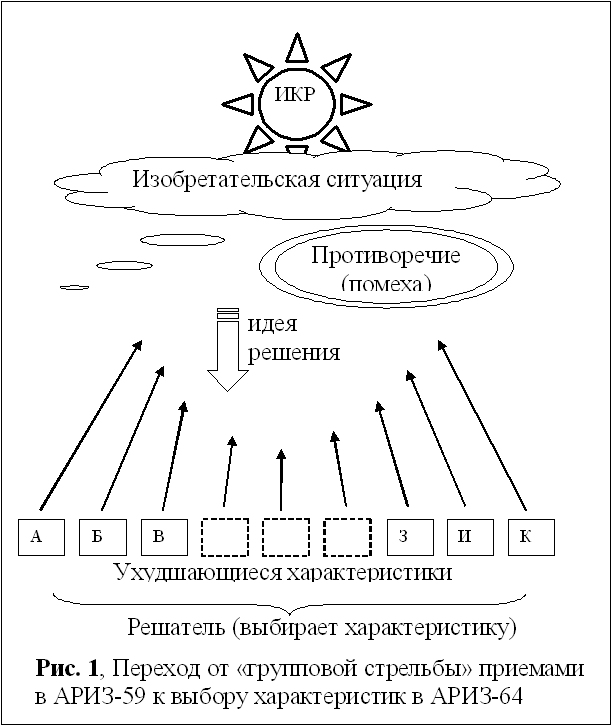
\includegraphics[width=.7\textwidth]{./16.jpg}
\end{center}

Все это должно было способствовать укреплению веры в работоспособность приемов
у пользователей. Правда, произошло значительное понижение их статуса:

Из «\textbf{Решателей, перебирающих по очереди все приемы}», пользователи АРИЗ
опускались до ранга «\textbf{Решателей, выбирающих ухудшаемые
  характеристики}».  По крайней мере, визуально.

В основу нового инструмента был заложен стандартный психологический эффект: С
введением предварительного отсева приемов ответственность Решателя за их выбор
(вернее, за правильный перебор) резко снижалась. Теперь забота о выборе
приемов как бы перешла в прошлое надсистемы (АРИЗ и его автор), стала решаться
«заранее». Она перекладывалась на Составителя Таблицы, недвусмысленно
гарантирующего успех при использовании лишь ограниченного числа приемов,
связанных с ухудшающейся характеристикой. Соответственно должна была
многократно возрастать вера в успешность «избранной» группы приемов. Они
попросту не могли не срабатывать. Не имели права.

О том, что в 1961 году Альтшуллер рекомендовал составление индивидуальной
таблицы каждому пользователю, предпочиталось больше не напоминать.

Каким именно образом автор Таблицы подбирал те или иные приемы, было его
собственным Know-how. Это уже не должно было волновать Решателя, который
отныне мог спокойно сконцентрироваться на более тщательном обдумывании лишь
нескольких табличных «избранников». Значительная важность придавалась теперь
«правильному определению» ухудшающейся характеристикой. Именно в сторону этого
решения перемещался центр тяжести будущей улучшенной оперативной стадии.

Раньше использование приемов напоминало Сизифов труд, узаконенный в последнем
шаге оперативной стадии АРИЗ-59 и АРИЗ-61:
\begin{quote}
  «Возвращение (в случае непригодности всех рассмотренных приемов) к исходной
  задаче и расширение ее условий, т. е. переход к другой, более общей задаче».
\end{quote}
Иными словами, Решатель обязывался перебирать все приемы «до победного конца»
или до полного поражения. И неоднократно, если понадобится.

Общее число приемов возросло против 1961 года в несколько раз. Перебирать их
стало невозможно уже исходя из основных принципов борьбы с МПиО. Но с приходом
Таблицы эта необходимость отпадала сама собой. Зато относительная
«прицельность» использования каждого из приемов в отдельности повысилась
многократно.

Но самым, пожалуй, важным качеством будущего инструмента -- с точки зрения
адаптации методики к производственным условиям -- становилось значительное
снижение затрат времени на прохождение части оперативной стадии, связанной с
«упорядоченными» приемами. Прежний страх перед тем, что, несмотря на высокую
стоимость анализа (как уже упоминалось, при 16 приемах он составлял от 4-х до
8-ми часов рабочего времени), он может завершиться неудачей, отступал.
Утомительная и напряженная процедура прохождения «приемной» стадии теперь
превращалась в приятную тренировку ума и сообразительности на час-полтора, не
более.

\subsection*{Облегчение оперативной стадии}

Плоская иллюстрированная матрица, явившаяся первой документально
подтвержденной графической попыткой Альтшуллера упорядочить применение
собранных к тому времени изобретательских принципов, получила двойное
название:

В приложении к книге она была озаглавлена «\textbf{Основные приемы устранения
  технических противоречий}» (Рис. 2 Основные приемы устранения технических
противоречий).

\begin{center}
  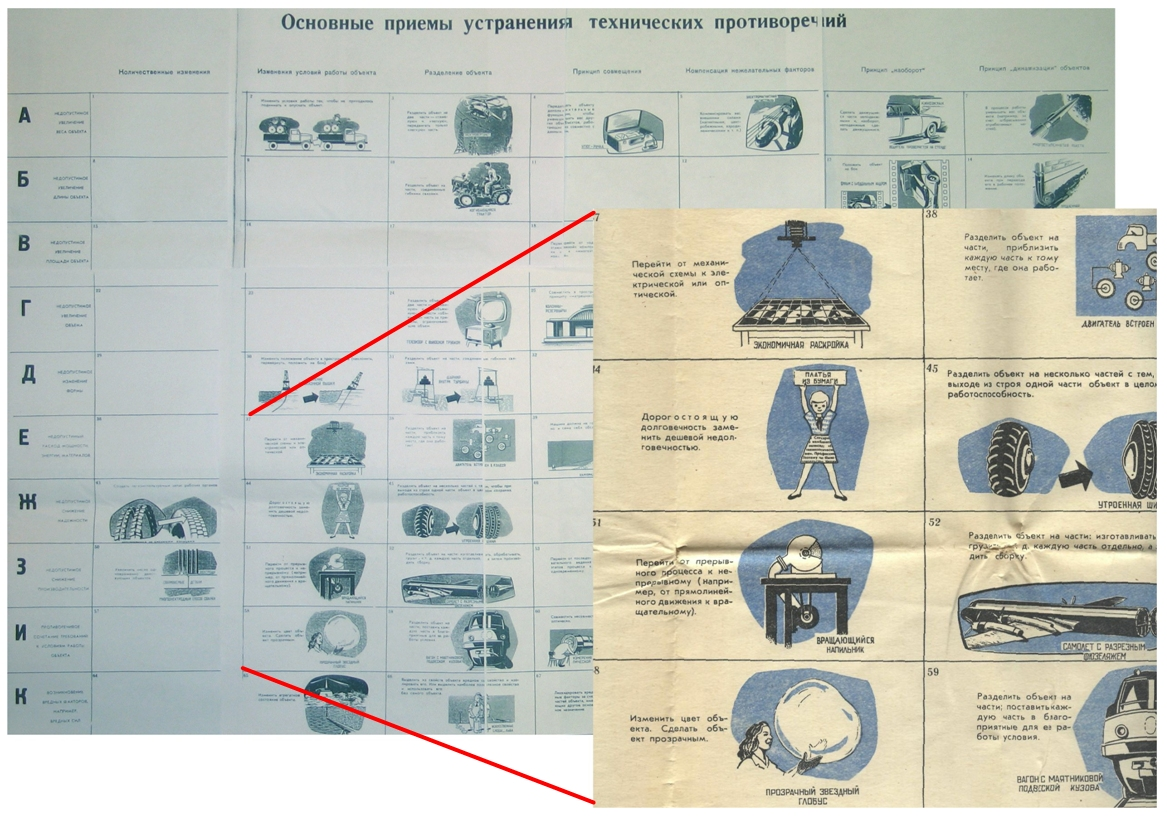
\includegraphics[width=.7\textwidth]{./17.jpg}
\end{center}

В более поздних разъяснениях к истории развития АРИЗ сам Альтшуллер называл ее
«\textbf{Впервые составленной таблицей групп приемов}» \cite{Altshuller1986a}.

Возможно, именно благодаря этому разночтению позднее распространилось
убеждение в том, что «первая Таблица» была введена уже в АРИЗ-64.

Она еще не предлагала готовые наборы приемов для различных конфликтующих пар.
Да и понятие «конфликтная пара» для работы с нею еще не требовалось. В ней
демонстрировались лишь принципиальные возможности применения отдельных приемов
для \textbf{устранения} «помехи» -- недопустимого ухудшения одной из десяти
сформулированных технических характеристик. Оставалось неясным и то, что же
подразумевалось под этим -- предотвращение, компенсация, преобразование или
какой-то другой вид \textbf{устранения} технических противоречий.

Собственно техническое противоречие в его привычной для нас сегодня двойной
форме, таким образом, здесь еще не формулировалось, а лишь подразумевалось.
Выбор приема осуществлялся «скрещиванием» в Таблице исходной ухудшаемой
характеристики с основными изобретательскими принципами.

В отличие от трех своих последовательниц, эта Таблица была, скорее, первой
пробой пера. Но вопрос о ее включении в АРИЗ представлялся практически
решенным:
\begin{quote}
  «Таблица предназначена для того, чтобы \textbf{облегчить оперативную стадию
    творческого процесса}. Анализ выявляет помеху, то есть присущее задаче
  техническое противоречие. После этого надо обратиться к таблице и проверить
  возможность устранение помехи приемами, указанными в соответствующем
  горизонтальном ряду». \cite{Altshuller1964}
\end{quote}
Все же избранный подход оставался кустарным и недостаточно убедительным:
\begin{quote}  
  «Помните, что типовые приемы сформулированы в общем виде. Конкретное же
  противоречие, с которым вы будете сталкиваться при решении задач, имеет
  индивидуальные особенности. Типовые приемы подобны готовому платью. Их надо
  подогнать, учитывая индивидуальные особенности, индивидуальные требования».
\end{quote}
В чем именно выражалась и во что выливалась «подгонка готового платья», так и
осталось неизвестным.

Принципиальная возможность использования всех возможных вариантов не
исключалась, но заполненными были только 40 полей из 70 возможных. Сам
Альтшуллер объяснял такое избирательное заполнение клеток нежеланием
перегружать Таблицу приемами второстепенного значения:
\begin{quote}  
  «Некоторые из них оставлены незаполненными. Можно, конечно, сформулировать
  приемы и для этих клеток. Но тогда типовые сильные приемы затеряются среди
  \textbf{слабых} приемов, \textbf{редко} используемых на практике».
\end{quote}
Зато каждый указанный прием сопровождался примером, снабженным отдельным
рисунком:
\begin{quote}  
  «Типовые приемы проиллюстрированы в таблице конкретными примерами.
  Разумеется, каждый пример поясняет лишь часть той общей идеи, к которой он
  относится. Примеры говорят о наглядных, но конкретных случаях. В то время
  как \textbf{каждый прием отображает общий принцип}».
\end{quote}
Впрочем, Альтшуллер и не скрывал того, что использование приемов на практике
является скорее искусством (может быть, даже Великим Искусством), чем легко
изучаемым ремеслом:
\begin{quote}  
  «Мастерство изобретателя на этом этапе работы заключается в умении гибко
  пользоваться идеями, содержащимися в общих формулах приемов».
\end{quote}
Наиболее перспективным -- по числу выявленных и применений -- представлялся
принцип «Разделение объекта» (тот самый шаг-выскочка, лишь недавно
«проклюнувшийся» в АРИЗ-61 с четырьмя новыми приемами). В девяти случаях из
десяти возможных этот принцип позволял устранять «помеху» (недопустимое
ухудшение технической характеристики) на пути к ИКР.

А вот «Количественные изменения», большие надежды на которые возлагались еще в
первых вариантах АРИЗ, помогали теперь только в двух случаях. В последующих
Списках и Таблицах этот принцип уже не встречался, а использованные для него
ранее примеры (Рис. 3 Приемы из «утерянного колена» -- Количественные изменения)
можно было легко перераспределить между другими приемами. В том, что уже на
основании рисунков к примерам каждый начинающий тризовец найдет им новые
применения, сомневаться не приходится.
\begin{center}
  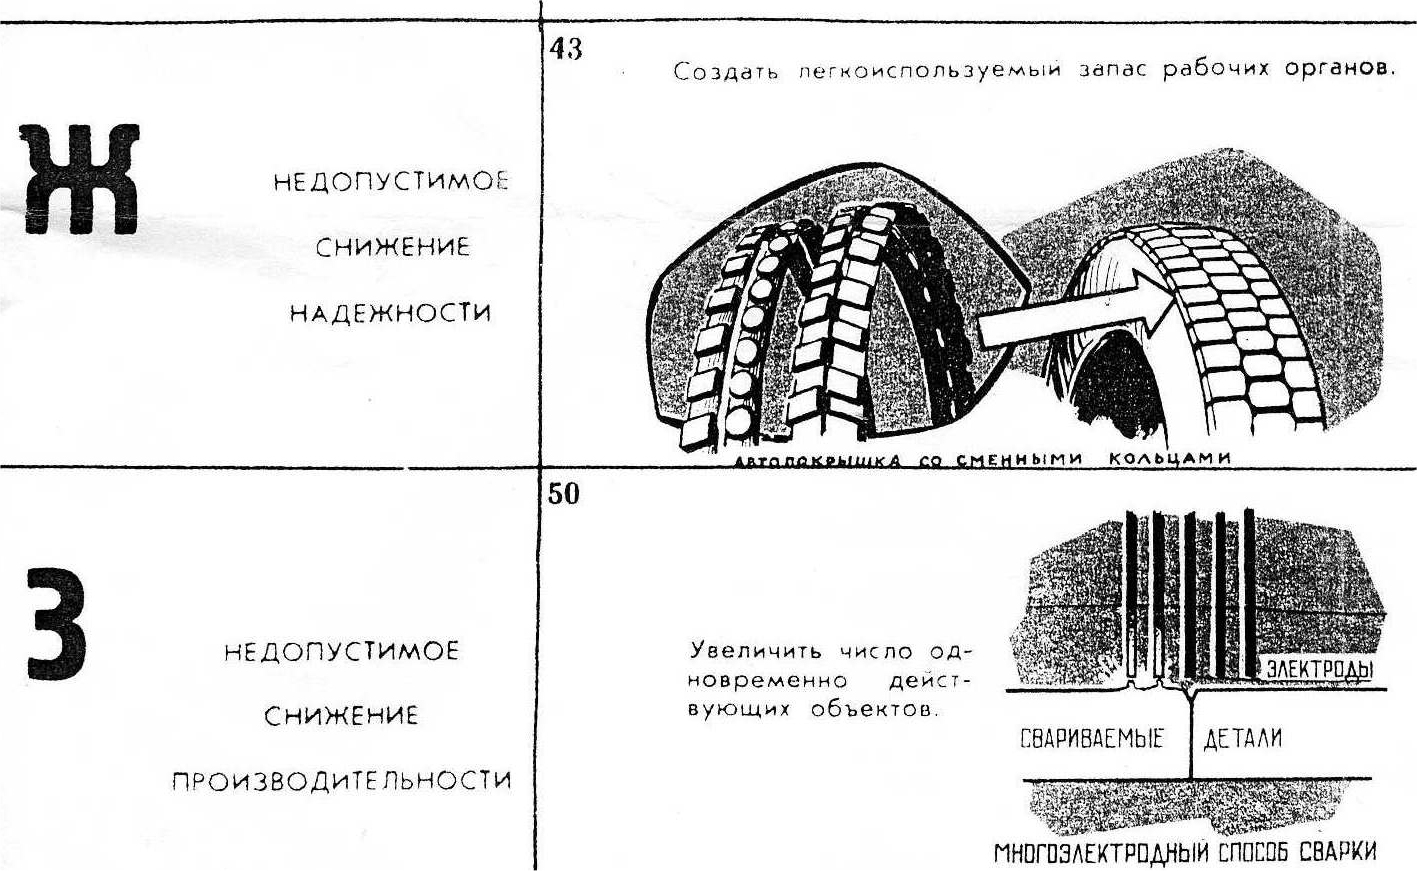
\includegraphics[width=.8\textwidth]{./18.jpg}
\end{center}

Возможно, именно несовершенство первой «таблицы групп приемов» явилось
причиной того, что Альтшуллер воздержался от непосредственного включения ее в
АРИЗ-64.  Как и того, что сам автор о ней позднее почти не упоминал.

\subsection*{Немного статистики}

Объемы статистических данных, легших в основу первой Таблицы Альтшуллера,
достоверно не известны. Можно лишь сослаться на выдержку из статьи 1959 года:
\begin{quote}  
  «Найти эти закономерности было нелегко. Мы искали их в истории техники, в
  описаниях сотен, тысяч изобретений, в воспоминаниях великих изобретателей, а
  главное -- \textbf{в огромном опыте, накопленном советскими новаторами}»
  \cite{Altshuller1959}.
\end{quote}
Более конкретные цифры появились в книге «Как научиться изобретать»
\cite{Altshuller1961}: «Работа над созданием такой методики была начата мною в
1946 году. …  Уже в первые три года работы (то есть за время до первого ареста
Альтшуллера и Шапиро -- Л.Ш.) были проанализированы 4\,000 описаний различных
изобретений».

Если исходная база данных для «впервые составленной таблицы групп приемов»
достоверно неизвестна, то можно провести анализ ее самой. Весьма поучительной
представляется приведенная ниже сравнительная таблица.

В ней перечислены приемы в составе шагов АРИЗ-61 и Способы устранения ТП в
Таблице-1964. Жирным шрифтом здесь выделены те приемы, которые в той или иной
форме перешли в состав Таблицы из АРИЗ-61. Или хотя бы узнаются в ней.

Подчеркиванием выделены группы приемов, «свернутые» в АРИЗ-64 в первый шаг
(информационную базу Таблицы). Неподчеркнутыми представлены группы приемов,
оставшиеся в АРИЗ-64 формально самостоятельными.

Казалось бы, в Таблице-1964 мы должны встретить все тринадцать приемов из
первых двух групп АРИЗ-61. Объединенные теперь в первом шаге АРИЗ-64, они
должны были составить, в результате объединения шагов, информационную базу
Таблицы. Но таких приемов оказалось лишь восемь.

Пять приемов из первых двух групп АРИЗ-61 (выделены курсивом) исчезли целиком
и полностью. «Потерялись» три приема на изменение -- материала, температуры,
давления. Выделение «необходимой и достаточной» части, как и Разделение
объекта на одинаковые части тоже потеряли свою актуальность и в Таблицу не
вошли.  Зато в нее добавились сразу тридцать два (32!) большей частью
принципиально новых Способа устранения ТП.

\begin{center}
  \begin{tabular}{|p{.35\textwidth}|p{.35\textwidth}|p{.15\textwidth}|}\hline
    \multicolumn{3}{|c|}{Сравнительная таблица приемов (1961) и Способов
      устранения ТП (1964)} \\\hline
    Приемы в составе шагов АРИЗ-61& Способы устранения ТП в Таблице-1964&
Номер клетки (способа)\\\hline
Изменение размеров. & Изменить условия работы так, чтобы не поднимать и не
опускать объект.& 2\\\hline
Изменение формы.& Разделить объект на две части -- «тяжелую» и «легкую»,
передвигать только «легкую» часть.& 3\\\hline
Изменение материала. & Передать объекту дополнительные функции, чтобы
уменьшить вес других объектов, работающих совместно с данным. & 4\\\hline
Изменение температуры. & Компенсировать вес внешними силами (магнитными,
центробежными, аэродинамическими и т.п.). & 5\\\hline
Изменение давления. & Сделать движущиеся части неподвижными и, наоборот,
неподвижные -- движущимися. & 6\\\hline
Изменение скорости.  & Уменьшить -- в процессе работы -- вес объекта
(например, за счет отбрасывания отработанных частей). & 7\\\hline
Изменение окраски.  & Разделить объект на части, соединенные гибкими
связями. & 10 \\\hline
Изменение взаимного расположения частей.  & Положить объект на бок(+) &
13\\\hline
Изменение режима работы частей с целью максимальной их нагрузки.  & Изменить
длину объекта при переводе его в рабочее положение. & 14\\\hline
Выделение «слабой» части.  & Перейти от «одноэтажной» компоновки к
«многоэтажной« & 18\\\hline
Выделение «необходимой и достаточной» части. & Изменять в процессе работы
площадь объекта. & 21\\\hline
  \end{tabular}

  \begin{tabular}{|p{.35\textwidth}|p{.35\textwidth}|p{.15\textwidth}|}\hline
Разделение объекта на одинаковые части. & Разделить объект на две части --
«объемную» и «необъемную». Вывести «объемную» часть за пределы, ограничивающие
объем & 24\\\hline
Разделение объекта на разные по функции части & Совместить в пространстве
несколько объемов (принцип «матрёшки«). & 25\\\hline
Изменение параметров среды. & Изменить объем при переводе объекта в рабочее
положение & 28\\\hline
Замена среды. & Изменить положение объекта в пространстве (наклонить,
перевернуть, положить на бок)(+) & 30\\\hline
Разделение среды на несколько частичных сред. & Разделить объект на части,
соединенные гибкими связями. & 31\\\hline
Использование внешней среды для выполнения полезных функций. & Создать
предварительное изменение формы, противоположное недопустимому. & 33\\\hline
Установление взаимосвязи между ранее независимыми объектами, участвующими в
выполнении одной работы. & Выполнить объект из материала, допускающего
изменение формы при работе. & 34\\\hline
Устранение одного объекта за счет передачи его функций другому объекту. &
Выполнить объект из материала, допускающего изменение формы при работе. &
35\\\hline
Увеличение числа объектов, одновременно действующих на ограниченной площади,
за счет использования свободной обратной стороны этой площади. & Перейти от
механической схемы к электрической или оптической & 37\\\hline
&Разделить объект на части, приблизить каждую часть к тому месту, где она
работает &38\\\hline
&Машина должна не только выполнять основную работу, но и сама себя
обслуживать &39\\\hline
&Компенсировать расход энергии получением какого-либо дополнительного эффекта
&40\\\hline
&Перейти от непрерывной подачи мощности к периодической, например, импульсной.
&42\\\hline
&Создать легко используемый «запас» рабочих органов. & 43\\\hline
  \end{tabular}

  \begin{tabular}{|p{.35\textwidth}|p{.35\textwidth}|p{.15\textwidth}|}\hline
&Дорогостоящую долговечность заменить дешевой недолговечностью. & 44\\\hline
&Разделить рабочий орган на несколько частей с тем, чтобы, при выходе из строя
одной части, объект в целом сохранял работоспособность.  & 45\\\hline
&Увеличить число одновременно действующих объектов.  & 50\\\hline
&Перейти от прерывного процесса к непрерывному (например, от прямолинейного
движения к вращательному) & 51\\\hline
&Разделить объект на части; изготовлять каждую часть отдельно, затем
производить сборку. & 52\\\hline
&Перейти от последовательного ведения этапов процесса к одновременному. &
53\\\hline
&Изменить цвет объекта. Сделать объект прозрачным. & 58\\\hline
&Разделить объект на части: поставить каждую часть в благоприятные для ее
работы условия. & 59\\\hline
&Совместить несовместимое оптически & 60\\\hline
&Объект должен менять свои свойства при изменении условий работы & 63\\\hline
&Изменить агрегатное состояние объекта & 65\\\hline
&Выделить из свойств объекта вредное свойство и изолировать его. Или выделить
наиболее полезное свойство и использовать его без самого объекта. & 66\\\hline
&Ликвидировать вредные факторы за счет частей объекта, имеющих другое основное
назначение & 67\\\hline
  \end{tabular}

  \begin{tabular}{|p{.35\textwidth}|p{.35\textwidth}|p{.15\textwidth}|}\hline
&Компенсировать вредные факторы за счет самих этих факторов (клин клином).
Использовать вредные факторы для выполнения полезной работы. & 68\\\hline
&Усилить вредные факторы настолько, чтобы они перестали быть вредными. &
69\\\hline
  \end{tabular}
\end{center}

Таким образом, общее число Способов устранения технического противоречия во
«впервые составленной Таблице групп приемов» 1964 года составило ровно сорок.

Это число поначалу сбивает с толку. Ведь сегодня известно, что все 40 типовых
приемов появились впервые в Таблице образца 1971 года.

Тщательное сравнение Способов устранения ТП в Таблице-1964 со списком 40
типовых приемов Таблицы в АРИЗ-71 не оставляет сомнения в простом совпадении
чисел: В Таблице-1964 в той или иной степени «проявляются» (с учетом здоровой
доли субъективности автора статьи) только 26 «классических» типовых приемов,
приведенных ниже в порядке возрастания номеров:

\paragraph{«Классические» типовые приемы, узнаваемые в Таблице-1964 как
  Способы устранения технических противоречий}
\begin{itemize}
\item[1.] Принцип дробления
\item[2.] Принцип вынесения
\item[3.] Принцип местного качества
\item[6.] Принцип универсальности
\item[7.] Принцип «матрешки«
\item[8.] Принцип антивеса
\item[9.] Принцип предварительного антидействия
\item[12.] Принцип эквипотенциальности
\item[13.] Принцип «наоборот«
\item[15.] Принцип динамичности
\item[16.] Принцип частичного или избыточного действия
\item[17.] Принцип перехода в другое измерение
\item[19.] Принцип периодического действия
\item[20.] Принцип непрерывности полезного действия
\item[21.] Принцип проскока
\item[22.] Принцип «обратить вред в пользу«
\item[23.] Принцип обратной связи
\item[25.] Принцип самообслуживания
\item[26.] Принцип копирования
\item[30.] Использование гибких оболочек и тонких пленок
\item[32.] Принцип изменения окраски
\item[35.] Принцип изменения агрегатного состояния
\end{itemize}

Несколько смущает только одно обстоятельство. Работа эта велась в
несвойственной для Альтшуллера атмосфере секретности; Информация о
промежуточных результатах или источниках получения новых приемов не
встречается в публикациях Генриха Сауловича 1961--1963 годов.

\subsection*{АРИЗ подстраивается под Таблицу}

Ограниченные возможности полосы не дают возможности провести сравнение всех
ранних версий АРИЗ. Поэтому попытаемся провести сравнительный анализ только
основных его «дотабличных» вариантов. Для удобства сравнения одинаковые
смысловые шаги в них расположены на одном уровне.

\begin{center}
  \begin{tabular}{|p{.3\textwidth}|p{.3\textwidth}|p{.3\textwidth}|}\hline
АРИЗ-59 \cite{Altshuller1959} & АРИЗ-61 \cite{Altshuller1961} & АРИЗ-64
\cite{Altshuller1964} \\\hline
\textbf{Оперативная Стадия} (Устранение условий, вызывающих причину
технического противоречия путем внесения изменений в одну из частей машины.)
& \textbf{Оперативная Стадия} & \textbf{Оперативная Стадия}\\\hline

\textbf{Первый шаг}. (59.1) & (61.2) & \multirow{2}{*}{\textbf{Первый шаг}.
  (64.2)} \\\hline
x & \textbf{Второй шаг}. (61.3) \\\hline
  \end{tabular}
\end{center}


\begin{thebibliography}{xxx}
\bibitem{Altshuller1956} Г.С. Альтшуллер, Р.Б. Шапиро. О психологии
  изобретательского творчества.  Вопросы психологии, 1956, № 6, стр. 37-49.
  \url{http://www.altshuller.ru/triz0.asp}
\bibitem{Altshuller1959} Г.С. Альтшуллер, Р.Б. Шапиро. Изгнание шестикрылого
  серафима. Изобретатель и рационализатор, 1959. № 10.
  \url{http://www.altshuller.ru/triz12.asp}
\bibitem{Altshuller1961} Г.С. Альтшуллер. Как научиться изобретать. Тамбов:
  Книжное издательство, 1961.  \url{http://www.altshuller.ru/triz/triz49.asp} 
\bibitem{Altshuller1963} Г.С. Альтшуллер. Как работать над изобретением.
  \emph{Азбука рационализатора}, Сост. Б. Зубков, Ю. Медведев, С. Муслин. --
  Тамбов: Кн. изд-во, 1963.
\bibitem{Altshuller1964} Г.С. Альтшуллер. Основы изобретательства. – Воронеж:
  Центрально-черноземное книжное издательство, Воронеж, 1964.
  \url{http://www.altshuller.ru/triz/ariz64.asp}
\bibitem{Altshuller1965} Г.С. Альтшуллер. Внимание: алгоритм изобретения!,
  Технико-экономические знания: приложение к «Экономической газете»,
  01.09.1965, -- Вып. 27(41).
\bibitem{Altshuller1971} Г.С. Альтшуллер.  Алгоритм решения изобретательских
  задач АРИЗ-71. – Баку: ОИИТ при ЦК ЛКСМ Азербайджана и Азербайджанском РС
  ВОИР, 1971. \url{http://www.altshuller.ru/triz/ariz71.asp}
\bibitem{Altshuller1974} Г.С. Альтшуллер. Планы занятий на первом курсе
  АзОИИТ.  1973--74. \url{http://www.altshuller.ru/engineering6.asp}.
\bibitem{Altshuller1975} Г.С. Альтшуллер, Г.Л. Фильковский. Современное
  состояние Теории Решения Изобретательских Задач. 1975.
  \url{http://www.altshuller.ru/triz2.asp}.
\bibitem{Altshuller1979} Г.С. Альтшуллер. Творчество как точная наука: Теория
  решения изобретательских задач. М.: Сов. радио, 1979.
\bibitem{Altshuller1985} Г.С. Альтшуллер. Письмо 19.  31.01.1985.
  \url{https://www.altshuller.ru/corr/correspondence1.asp#19}
\bibitem{Altshuller1986} Г.С. Альтшуллер. Жизнь Человека 1-Ч-502, рассказанная
  Игорю Верткину, 1985-1986.
  \url{https://www.altshuller.ru/interview/interview5.asp}.
\bibitem{Altshuller1986a} Г.С. Альтшуллер.  История Развития АРИЗ (конспект).
  1986.  \url{http://www.altshuller.ru/triz/ariz-about1.asp}
\bibitem{Altshuller1994} Г.С. Альтшуллер, И.М. Верткин. Как стать гением:
  Жизненная стратегия творческой личности. -- Минск, Беларусь, 1994.
  \url{http://www.altshuller.ru/trtl/heretic2.asp}
\bibitem{Altshuller1996} Г.С. Альтшуллер. Ответы на вопросы Джеймса Ковалика.
  16.06.1996.  \url{https://www.altshuller.ru/interview/interview4.asp}.
\bibitem{Amnuel964} П. Амнуэль. Старик Жюль Верн и космическая эра. Молодежь
  Азербайджана, Баку 1964.  \url{http://www.fandom.ru/}.
\bibitem{Bachmatov1961} Р. Бахтамов. Изгнание шестикрылого серафима, М.:
  Детгиз, 1961.  
\bibitem{Blaesing2001} Jürgen P. Bläsing, Walter Brunner. TRIZ. Von der
  Theorie zur Praxis. Für TRIZ Moderatoren und TRIZ Teams. Mit der
  Konflikt-Matrix in DIN A2, Ausgabe 2001.
\bibitem{Dworschak2005} Manfred Dworschak. Zwergenarmeen im Kopf. Der
  Spiegel, 30/2005, S. 114.
\bibitem{Filkovsky2006} Г. Фильковский (2006). «Горин -- автор идеи
  физического противоречия ???!!!».
  \url{http://www3.sympatico.ca/karasik/GF_re_gorin_claim.html}
\bibitem{Gimpel2000} Bernd Gimpel, Rolf Herb, Thilo Herb. Ideen finden,
  Produkte entwickeln mit TRIZ. Hanser Verlag, 2000.
\bibitem{Herb2000} Rolf Herb, Thilo Herb, Veit Kohnhauser. TRIZ, der
  systematische Weg zur Innovation. Verlag Moderne Industrie, 2000.deen finden,
  Produkte entwickeln mit TRIZ. Hanser Verlag, 2000.
\bibitem{Jacobson1934}  П.М. Якобсон. Процесс творческой работы изобретателя.
  1934. 
\bibitem{Korneev1962} С.Г. Корнеев, Тайны творчества, Тамбов, 1962,
  Библиотечка новатора.  \url{https://www.metodolog.ru/00696/00696.html} 
\bibitem{Korneev1964} С.Г. Корнеев, Алгебра и гармония, Тамбов, 1964.
  (Библиотечка новатора; Вып. 2),
  \url{http://www.metodolog.ru/00630/00630.html}
\bibitem{Korolyev1998} В.А. Королёв. Современные тенденции развития АРИЗ.
  25.01.1998. \url{http://www.triz.org.ua/data/w55.html}
\bibitem{Kudryavtsev} А.В. Кудрявцев. Как выбирать приемы для решения.
  Учебник по ТРИЗ. гл. 8.  \url{http://metodolog.ru/00088/00088.html}
\bibitem{Leon2005} Noel Leon, Jose Jesus Martinez, Carlos Castillo.
  Methodology for the Evaluation of the Innovation Level of Products and
  Processes. TRIZ Journal 10/2005.
\bibitem{Livotov2004} P. Livotov. TRIZ im Innovationsprozess. Konstruktion \&
  Engineering, 03/2004.
\bibitem{Livotov2005} P. Livotov, D. Murnikov. Innovation als Prozess. 
  4. TRIZ-Kongress, Frankfurt, 29. Juni 2005. 
\bibitem{Mann2005a} Darrell Mann, Conall Ó Catháin.  Using TRIZ in
  Architecture: First Steps. TRIZ Journal 11/2005.
\bibitem{Mann2005b} Darrell Mann, Chris Bradshaw. Design for Wow 2 – Music.
  TRIZ Journal 10/2005.
\bibitem{MATRIZ2003} МА ТРИЗ. Проект Положения о многоступенчатой аттестации
  пользователей и сертификации специалистов Международной Ассоциации ТРИЗ.
  Принято на заседании Президиума МА ТРИЗ, 26 июня 2003 г.
  \url{https://triz-summit.ru/triz/history/300029/matriz-2003/300314/300315/}.
\bibitem{Murashkovsky2003} Письмо от Ю.С. Мурашковского. 03.10.2003.
  \url{https://subscribe.ru/archive/science.natural.triz/200310/03201643.html}.
\bibitem{Murashkovsky2006} Ю.С. Мурашковский, Детская болезнь
  «ниспровержизма». 22.03.2006, не опубликован.
  \url{https://subscribe.ru/archive/science.natural.triz/200310/03201643.html}.
\bibitem{OrlovNN} В. Орлов, Трактат о вдохновении, рождающем великие
  изобретения.  \url{https://www.metodolog.ru/00193/00193.html}
\bibitem{Salamatov1992} Ю.П.Саламатов. Современное состояние и проблемы
  развития ИМ-ТРИЗ-технологии. Минск, 19-21 мая 1992 г.
  \url{http://www.triz-guide.com/publicat/articles/article7.html}
\bibitem{Shub2004} Л. Шуб. Особенности распространения и видоизменения ТРИЗ в
  центральной Европе (1998--2004).
  \url{http://metodolog.ru/00452/00452.html}.
\bibitem{Shub2006} Л. Шуб. Сравнительная таблица изменений и перемещений в
  ранних версиях АРИЗ. \url{https://metodolog.ru/00908/00908.pdf}
\bibitem{Sietmann2001} Richard Sietmann. Erfinden nach Plan. c't -- Magazin
  fur Computertechnik 23/01, Seite 96.
\bibitem{Stuart2005} Jack Stuart. Transactional TRIZ, Theory, Application, and
  Execution, Part II: The Contradiction Matrix. TRIZ Journal 10/2005.
\bibitem{Teufelsdorfer1998} A. Teufelsdorfer, A.  Conrad. Kreatives Entwickeln
  und innovatives Problemlösen mit TRIZ/TIPS, Publicis MCD Verlag, Erlangen
  und München 1998.
\bibitem{Terninko1998} John Terninko, Alla Zusman, Boris Zlotin. TRIZ -- Der
  Weg zum konkurrenzlosen Erfolgsprodukt. Verlag Moderne Industrie, 1998.
\bibitem{ZlotinZusmanNN} Б. Злотин, А. Зусман, «О попытке документирования
  истории ТРИЗ»,
  \url{http://www.trizscientific.com/TRIZ_sci/history/history_main_r.htm}
\end{thebibliography}


\end{document}

%=============================================================

Проверка возможности разделения объекта на независимые части.
1. Выделение «слабой» части.
2. Выделение «необходимой и достаточной» части.
3. Разделение объекта на одинаковые части.
4. Разделение объекта на разные по функции части.
Второй шаг. Проверка возможных изменений во внешней среде: изменение параметров среды, замена среды, использование среды для выполнения полезных функций. 	Третий шаг. Проверка возможных изменений во внешней (для данного объекта) среде.
1. Изменение параметров среды.
2. Замена среды.
3. Разделение среды на несколько частичных сред.
4. Использование внешней среды для выполнения полезных функций. 	Второй шаг: Проверить возможные изменения в среде, окружающей объект, и в других объектах, работающих совместно с данным.
Третий шаг. Проверка возможных изменений в других (соседних для данного) объектах: установление взаимосвязи с соседними объектами, изменение характера ранее установленной взаимосвязи, отказ от соседнего объекта за счет переложения его функций на данный объект. 	Четвертый шаг. Проверка возможных изменений в соседних (т.е. работающих совместно с данным) объектах.
1. Установление взаимосвязи между ранее независимыми объектами, участвующими в выполнении одной работы.
2. Устранение одного объекта за счет передачи его функций другому объекту.
3. Увеличение числа объектов, одновременно действующих на ограниченной площади, за счет использования свободной обратной стороны этой площади.
Четвертый шаг. Исследование прообразов из других отраслей техники (поставить вопрос: «Как данное противоречие устраняется в других отраслях техники?«) 	Пятый шаг. Исследование прообразов из других отраслей техники (поставить вопрос: как данное противоречие устраняется в других отраслях техники?). 	Третий шаг: Перенести решение из других отраслей техники (ответить на вопрос: «Как решаются в других отраслях техники задачи, подобные данной?«).

Четвертый шаг: Применить «обратные» решения (ответить на вопрос: «Как решаются в технике задачи, обратные данной, и нельзя ли использовать эти решения, взяв их, так сказать, со знаком минус?«).
Пятый шаг. Исследование прообразов в природе (поставить вопрос: «Как данное противоречие устраняется в природе?«) 	Шестой шаг. Исследование прообразов в природе (поставить вопрос: как данное противоречие устраняется в природе?). 	Пятый шаг: использовать «прообразы» природы (ответить на вопрос: «Как решаются в природе более или менее сходные задачи?«).
Шестой шаг. Возвращение (в случае непригодности всех рассмотренных приемов) к исходной задаче и расширение ее условий, то есть переход к другой, более общей задаче. 	Седьмой шаг. Возвращение (в случае непригодности всех рассмотренных приемов) к исходной задаче и расширение ее условий, т. е. переход к другой, более общей задаче. 	
Х

\paragraph{(59.1)}
Проверка возможных изменений в самом объекте (то есть в данной машине, данном
технологическом процессе и т. д.): изменение размеров, числа частей, формы,
взаимосвязи частей, материала, температуры, давления, скорости и т. д.

\paragraph{(61.2)}
Проверка возможных изменений в самом объекте (т. е. в данной машине, данном
технологическом процессе).
\begin{itemize}
\item[1.] Изменение размеров.
\item[2.] Изменение формы.
\item[3.] Изменение материала.
\item[4.] Изменение температуры.
\item[5.] Изменение давления.
\item[6.] Изменение скорости.
\item[7.] Изменение окраски.
\item[8.] Изменение взаимного расположения частей.
\item[9.] Изменение режима работы частей с целью максимальной их нагрузки.
\end{itemize}

\paragraph{(64.2)}
Проверить возможность устранения технического противоречия изменением данного
объекта (машины, механизма, процесса).

Х
	Второй шаг. Проверка возможности разделения объекта на независимые части.
1. Выделение «слабой» части.
2. Выделение «необходимой и достаточной» части.
3. Разделение объекта на одинаковые части.
4. Разделение объекта на разные по функции части.
Второй шаг. Проверка возможных изменений во внешней среде: изменение параметров среды, замена среды, использование среды для выполнения полезных функций. 	Третий шаг. Проверка возможных изменений во внешней (для данного объекта) среде.
1. Изменение параметров среды.
2. Замена среды.
3. Разделение среды на несколько частичных сред.
4. Использование внешней среды для выполнения полезных функций. 	Второй шаг: Проверить возможные изменения в среде, окружающей объект, и в других объектах, работающих совместно с данным.
Третий шаг. Проверка возможных изменений в других (соседних для данного) объектах: установление взаимосвязи с соседними объектами, изменение характера ранее установленной взаимосвязи, отказ от соседнего объекта за счет переложения его функций на данный объект. 	Четвертый шаг. Проверка возможных изменений в соседних (т.е. работающих совместно с данным) объектах.
1. Установление взаимосвязи между ранее независимыми объектами, участвующими в выполнении одной работы.
2. Устранение одного объекта за счет передачи его функций другому объекту.
3. Увеличение числа объектов, одновременно действующих на ограниченной площади, за счет использования свободной обратной стороны этой площади.
Четвертый шаг. Исследование прообразов из других отраслей техники (поставить вопрос: «Как данное противоречие устраняется в других отраслях техники?«) 	Пятый шаг. Исследование прообразов из других отраслей техники (поставить вопрос: как данное противоречие устраняется в других отраслях техники?). 	Третий шаг: Перенести решение из других отраслей техники (ответить на вопрос: «Как решаются в других отраслях техники задачи, подобные данной?«).

Четвертый шаг: Применить «обратные» решения (ответить на вопрос: «Как решаются в технике задачи, обратные данной, и нельзя ли использовать эти решения, взяв их, так сказать, со знаком минус?«).
Пятый шаг. Исследование прообразов в природе (поставить вопрос: «Как данное противоречие устраняется в природе?«) 	Шестой шаг. Исследование прообразов в природе (поставить вопрос: как данное противоречие устраняется в природе?). 	Пятый шаг: использовать «прообразы» природы (ответить на вопрос: «Как решаются в природе более или менее сходные задачи?«).
Шестой шаг. Возвращение (в случае непригодности всех рассмотренных приемов) к исходной задаче и расширение ее условий, то есть переход к другой, более общей задаче. 	Седьмой шаг. Возвращение (в случае непригодности всех рассмотренных приемов) к исходной задаче и расширение ее условий, т. е. переход к другой, более общей задаче. 	
Х


%===================================

Уже отмечалось, что в АРИЗ-64 произошло вынесение первого шага аналитической стадии и образование отдельной стадии -- «Уточнение формулировки задачи».

Наряду с этим, в АРИЗ-64 произошли и другие преобразования, так или иначе связанные с предстоящим введением Таблицы непосредственно в алгоритм. В значительной степени эти изменения определили и будущую политику развития ТРИЗ.

Во-первых, в оперативной стадии последовало бесследное и, на первый взгляд, парадоксальное исчезновение лишь недавно введенного в АРИЗ-61 второго шага вместе со всей группой «разделительных» приемов.

Вместо него появился новый четвертый шаг оперативной стадии:

    Применить «обратные» решения (ответить на вопрос: «Как решаются в технике задачи, обратные данной, и нельзя ли использовать эти решения, взяв их, так сказать, со знаком минус?«).

Этот шаг (пусть пока обще сформулированный) продолжил традицию поэтапного расширения АРИЗ за счет вновь наработанных приемов. За ним стояла новая, еще неразвернутая группа приемов с общей «философией«: Сделай наоборот!

Выделение «обратных» решений в отдельный логический шаг было не случайным. Как и выделение второго, «разделительного» шага в АРИЗ-61. Это еще больше подчеркнуло новизну и большой потенциал заложенных в новых шагах приемов.

Но периоды независимости новых групп приемов оставались недолгими. Так же как пропал из оперативной стадии «разделительный» шаг, суждено было и «наоборот«-шагу вскоре исчезнуть. Не успев «развернуться», он занял место в конце первого шага вновь созданной стадии «Уточнение условий задачи» в АРИЗ-68.

А свое «выставочное» место в оперативной стадии «наоборот«-шаг уступил в АРИЗ-68 следующей группе приемов. Очередным фаворитом стал четвертый шаг:

Проверка возможных изменений во времени.

Второе значительное изменение, отличающее АРИЗ-64 от его предшественников, выразилось в исчезновении последнего, седьмого шага оперативной стадии, до этого исправно работавшего в АРИЗ-59 и АРИЗ-61:

    Возвращение (в случае непригодности всех рассмотренных приемов) к исходной задаче и расширение ее условий, т. е. переход к другой, более общей задаче.

За этой не слишком обидной пропажей крылся, однако, поистине политический манифест: Отбросить все сомнения! Оперативная стадия обязана решать любую задачу!

Что же придало автору алгоритма такую безусловную уверенность? Что позволило ему утверждать, что уже одноразовый проход по оперативной стадии (с использованием всех предлагаемых приемов) будет достаточным для успешного решения любой поставленной задачи? Что до «возвращения к исходной задаче и расширение ее условий, т. е. переход к другой, более общей задаче» дело уже не дойдет?

Возможных ответов представляется несколько (с учетов вновь введенного «уточнения формулировки задачи«):

1. Альтшуллер обнаружил неисчерпаемый источник новых приемов, покрывающих все разнообразие известных технических решений, из которого он мог долговременно пополнять, расширять, обновлять и уточнять как «табличный» Список, так и АРИЗ.

2. Разрастание Списка приемов подтолкнуло его к идее о постепенном перераспределении приемов между различными «инструментами«: Таблицей, независимыми шагами оперативной стадии и начинавшимися разрабатываться операторами (по сути, «мини-оперативными стадиями» целевого назначения). Это позволяло значительно дольше и интенсивнее «играться» с различными приемами, не особенно рискуя оказаться в роли простого «переборщика вариантов».

3. Ему удалось «нащупать» идею нового механизма -- оператора для снятия психологической инерции, позволяющего создать у решателя ощущение ускоренного выбора наиболее удачных приемов из постоянно расширяющегося списка. Одновременно у решателя снижался страх ответственности за возможную неудачу.

В третьих, в АРИЗ-64 произошло не только радикальное «сворачивание» трех совсем недавно «развернутых» групп приемов, но и пока еще трудно объяснимое объединение двух из них в лаконичный второй шаг:

«Проверить возможные изменения в среде, окружающей объект (*3-й шаг в АРИЗ-61 -- Л.Ш.), и в других объектах, работающих совместно с данным (*4-й шаг в АРИЗ-61 -- Л.Ш.)».

Казалось бы, ничто не мешало Альтшуллеру, теперь уже единоличному автору АРИЗ, «сплавить» в составе АРИЗ-64 вместе все первые четыре шага (группы приемов) оперативной стадии из АРИЗ-61.

Следующее интересное новшество, касающееся будущей Таблицы, проявилось в подготовке к достижению идеального результата уже на четвертом шаге аналитической стадии:

«Определить, при каких условиях ничто не мешало бы получить идеальный результат. Ответить на вопрос: «При каких условиях исчезнет «помеха«?».

Собственно оперативная стадия началась с принципиально измененного первого шага:

«Проверить возможность устранения технического противоречия изменением данного объекта (машины, механизма, процесса)».

Таким образом, произошло многообещающее «сворачивание» в один шаг ставшей уже привычной «проверки изменений в самом объекте», представленной девятью приемами, и впервые введенной в АРИЗ-61 «проверки возможности разделения объекта на независимые части» с четырьмя приемами.

Новая формулировка первого шага стала недвусмысленным анонсом будущего «суперинструмента».

Наряду с основными указанными изменениями, АРИЗ-64 имел еще одну особенность, которую пока что можно отнести к числу курьезов. Прообразы природы, исследованию которых еще недавно посвящался вопрос «Как данное противоречие устраняется в природе?», были заключены в кавычки.

«Прообразы» природы (теперь уже на пятом шаге) приобрели теперь зримо второстепенное значение. И вопрос, относящийся к этим «закавыкам», стал звучать даже как-то небрежно:

«Как решаются в природе более или менее сходные задачи?«

Так постепенно задвигался в дальний угол, рискуя быть вытесненным из АРИЗ, шаг, стоявший в оперативной стадии 1956 года на первом месте. Лишь через четыре года в АРИЗ-68 он снова удостоился внимания автора и начал интенсивно «разрабатываться».

В заключение, следует особо подчеркнуть, что процедура «проверки возможности устранения технического противоречия изменением данного объекта» в АРИЗ-64 распространилась только на приемы из первого (изменения в самом объекте) и второго (разделения объекта) шагов. Третий и четвертый шаги АРИЗ-61 (соответственно, второй и третий шаги АРИЗ-59) в полном составе в этом процессе уже не участвовали.

Формально это, пионерское по открывающимся перспективам, введение в АРИЗ понятия «технического противоречия» произошло уже в АРИЗ-59 (как пояснение к сущности оперативной стадии):

«Устранение условий, вызывающих причину технического противоречия путем внесения изменений в одну из частей машины».

Но лишь в составе АРИЗ-64 оно придало оперативной стадии требуемую направленность и инструментальную окраску.

Укрепление позиции «технического противоречия» ознаменовало начало новой эры в развитии, как самого алгоритма, так и ТРИЗ в целом. За этим, пока еще общим и неотработанным понятием, как и за «проверкой возможности его устранения» теперь маячила «впервые составленная таблица групп приемов» Генриха Альтшуллера.

%=============================================================
 Часть 5

Минус первая Таблица (1963)

В предыдущей статье мы уделили внимание первой разработке Г. С. Альтшуллера в истории создания Таблицы. Вернее, той самой в 1964 году «впервые составленной таблице групп приемов», на которую Генрих Саулович сам же в дальнейшем и ссылается (Г. Альтшуллер, «История развития АРИЗ«).

На основании этих данных, доверяя точности и корректности автора «Истории развития АРИЗ», мы вправе допустить, что самим Альтшуллером никакие попытки по составлению Таблиц до 1964 года не предпринимались. А если предпринимались, то не Альтшуллером. Или не в ТРИЗ. Такое разделение противоречивых свойств позволяло бы допустить существование неких нетризных, «доисторических», неальтшуллеровских таблиц и до 1964 года.

Но вот в сборнике «Азбука рационализатора» [Азбука рационализатора, Сост. Б. Зубков, Ю. Медведев, С. Муслин. -- Тамбов: Кн. изд-во, 1963. -- 352 с. -- Гл. ХI. Г.С. Альтшуллер «Как работать над изобретением». -- С. 274 -- 304], изданном в Тамбове в 1963 году, мы обнаруживаем Таблицу, остававшуюся до сих пор неизвестной. Во всяком случае, неизвестной для широкой тризной общественности. В отличие от младшей сестренки-погодки, она еще не содержит рисунков и приведена в виде простого списка. В левой колонке -- типовые технические противоречия, обозначенные буквами от «А» до «К». В правой колонке -- опять же типовые способы устранения технических противоречий. Поясняющие рисунки к несколько приемам даны на отдельной странице.

Бросается в глаза отсутствие верхней горизонтальной оси, в которой годом позже были представлены (основные) принципы устранения технических противоречий, объединяющие приемы в семь групп. Именно эта ось-строка должна была придать вновь разработанной конструкции окончательно «типовой», табличный вид.

Читатель может возразить, мол, легко найти недостаток, когда знаком со всей дальнейшей историей развития. И все же, разделения на группы явно не хватает. Таких четко выраженных групп приемов уже в 1961 году было четыре. И в том, что их число за два года значительно возросло -- по крайней мере, до шести -- сомневаться не приходится. Ведь для одной из характеристик (А. «Недопустимое увеличение веса объекта«) нашлось сразу шесть Способов устранения технических противоречий, каждый из которых относится к самостоятельной группе. Но, может быть, автор Таблицы пока еще просто не знал, к каким именно группам или характеристикам следует отнести те или иные приемы?

В результате произошло (по крайней мере, визуальное) перераспределение Способов-приемов между ухудшающимися характеристиками, привязка к ним, а не к (основным) принципам устранения технических противоречий. И это в значительной степени изменило логику развития представления о механизме выбора «правильного» приема.

Другим внешним отличием Таблицы-1963 является «некруглое» число предлагаемых в ней приемов -- их в 1963 году было «только» 36 (в 1961 году приемов было 20, а в 1964 -- уже 40). Создается впечатление, что число выработанных Альтшуллером приемов растет последовательно неуклонно из года в год.

Но даже беглое сравнение с Таблицей-1964 показывает, что последняя образовалась вовсе не за счет простого дополнения своей предшественницы четырьмя новыми приемами. Процесс обновления был гораздо сложнее. Некоторые приемы образца 1963 года не были включены в следующий вариант, но нашли применение в более поздних Таблицах. К ним относится №32. «Изменить скорость процесса так, чтобы вредные факторы не успели проявиться». А отдельные приемы, такие как №15. «Разместить ограничители объема не снаружи, а, наоборот, внутри объекта», были удалены из списков уже раз и навсегда.

Вот что пишет об этой Таблице сам автор главы «Как работать над изобретением«:

«По меньшей мере, две трети изобретательских задач связаны с несколькими типами наиболее распространенных типовых противоречий. Для этих типовых противоречий можно указать и типовые способы их устранения (см. Таблицу 19)».

ТАБЛИЦА типовых технических противоречий и способов их устранения,
(Г.С. Альтшуллер «Как работать над изобретением», сб. «Азбука рационализатора», 1963)
Ухудшающаяся характеристика	Способы устранения технических противоречий (нумерация сплошная)
А. Недопустимое увеличение веса объекта 	1. Изменить условия работы так, чтобы центр тяжести объекта не перемещался в вертикальном направлении.
	2. Разделить объект на две части -- «тяжелую» и «легкую», передвигать только «легкую» часть.
	3. Передать объекту дополнительные функции, чтобы уменьшить вес других объектов, работающих совместно с данным.
	4. Компенсировать вес внешними силами (магнитными, центробежными, аэродинамическими и т. п.).
	5. Сделать движущиеся части неподвижными и, наоборот, неподвижные -- движущимися.
	6. Уменьшить -- в процессе работы -- вес объекта (например, за счет отбрасывания отработанных частей).
Б. Недопустимое увеличение длины объекта 	7. Изменить форму объекта.
	8. Разделить объект на части, соединенные гибкими связями.
	9. Изменить длину объекта при переводе его в рабочее положение.
В. Недопустимое увеличение площади объекта	10. Изменить положение объекта в пространстве.
	11. Перейти от «одноэтажной» компоновки к «многоэтажной».
	12. Изменять в процессе работы величину площади.
Г. Недопустимое увеличение объема 	13. Разделить объект на две части -- «объемную» и «необъемную». Вывести «объемную» часть за пределы, ограничивающие объем.
	14. Совместить в пространстве несколько объемов (принцип «матрёшки«).
	15. Разместить ограничители объема не снаружи, а, наоборот, внутри объекта.
	16. Перейти от фиксированного объема к переменному.
Д. Недопустимое изменение формы	17. Изменить размеры объекта.
	18. Разделить объект на гибко связанные части
	19. Создать предварительное изменение формы, противоположное недопустимому.
	20. Перейти от постоянной формы к переменной.
Е. Недопустимое повышение требуемой мощности (или энергии)	21. Допустить повышение требуемой мощности, пополнив ее недостаток из окружающей среды.
	22. Допустить повышенный расход мощности, но одновременно получить какой-то новый дополнительный эффект.
	23. Перейти от непрерывной подачи мощности к периодической, например, импульсной.
Ж. Недопустимое снижение надежности	24. Создать легко используемый «запас» рабочих органов.
	25. Разделить рабочий орган на несколько частей с тем, чтобы, при выходе из строя одной части, объект в целом сохранял работоспособность.
	26. Дорогостоящую долговечность заменить дешевой недолговечностью.
З. Недопустимое снижение производительности 	27. Увеличить число одновременно действующих объектов, перейти от прерывного процесса к непрерывному, например, от поступательного движения к вращательному
	28. Разделить объект на части; изготовлять каждую часть отдельно, затем производить сборку.
	29. Перейти от последовательного ведения этапов процесса к одновременному
И. Противоречивое сочетание требований к условиям работы объекта	30. Перевести объект (или часть) в другое агрегатное состояние
	31. Разделить объект на части: поставить каждую часть в оптимальные для нее условия
К. Возникновение вредных факторов, например, вредных сил 	32. Изменить скорость процесса так, чтобы вредные факторы не успели проявиться.
	33. Выделить из комплекса факторов единственно вредный и изолировать его.
	34. Компенсировать вредные факторы за счет самих этих факторов (клин клином). Использовать вредные факторы для выполнения полезной работы.
	35. Усилить вредные факторы настолько, чтобы они перестали быть вредными (например, шумный звук перевести в бесшумный ультразвук).
	36. Агрегатное состояние объекта на каждом этапе должно быть наивыгоднейшим.

Любопытными представляются рассуждения автора о стратегическом направлении в развитии ТРИЗ:

«Изобретательских задач бесчисленное множество. Количество же технических противоречий относительно невелико. Однако при современном развитии теории изобретательства еще нельзя дать общие правила, с помощью которых для каждой задачи удавалось бы сразу же найти соответствующий способ устранения технического противоречия. Потому на Оперативной стадии работы над изобретением приходится вести поиск. Но этот поиск ведется по рациональной системе, с использованием приемов, достаточных для большинства встречающихся на практике случаев».

Эти рассуждения отражают одновременно и прогрессивный ход мысли автора, и силу психологической инерции, из плена которой ему самому приходилось вырываться на каждом этапе развития методики, на каждом этапе собственной жизни.

Идея -- столь же гениальная, как и неуловимая -- по-прежнему витала в воздухе, не отваживаясь обрести свою постоянную телесную оболочку. Общих правил нет, но поиск все же следует вести по рациональной системе. Глядя на Таблицу и вспоминая о структуре списков приемов в 1961 и 1964 годах, нетрудно убедиться в том, что «рациональность» системы поиска имела новый смысл в каждом из вариантов Таблицы.

Альтшуллер не решился назвать или хотя бы оценить число технических противоречий, количество которых в 1963 году «относительно невелико». Представить себе, насколько же «невелико» может быть это число в действительности, он и сам еще не мог.

О своем будущем изобретении, позволяющем быстро и планомерно генерировать произвольное число «типовых технических противоречий», увеличивая их количество сначала до двухсот, затем до девятисот и, наконец, до полутора тысяч, автор Таблицы в 1963 году еще ничего не знал.

%=============================================================
Часть 6


Таблица, предложенная инженером Альтшуллером редактору Корнееву (1962)

«Таблица Альтшуллера вне подозрений!«

(приписывается Ю. Цезарю)

Пришло время вспомнить еще одно имя, до сих пор упоминавшееся лишь во второстепенных исторических материалах по ТРИЗ. Связать его с возникновением Таблицы все же можно -- по крайней мере, с высокой степенью вероятности.

«С 1961 г. работу по методике изобретательства энергично поддерживал Станислав Георгиевич Корнеев. Он был редактором, сумевшим преодолеть трудности выпуска методической литературы, затем -- организатором семинаров и, наконец, исследователем методики изобретательства. (Выделено нами -- Л.Ш.) С.Г. Корнеев отдал много сил этой работе. В 1964 г. он умер» [Альтшуллер Г.С., Планы занятий на первом курсе АзОИИТ, 1973 -- 74, http://www.altshuller.ru/engineering6.asp].

Об этом человеке, его жизни и творчестве, как и о его вкладе в развитие методики нам известно, к сожалению, пока еще очень немного:

«Редактор тамбовского книжного издательства. Первым из редакторов осознал значение ТРИЗ для человечества. Проделал большую работу по изданию книг и материалов по ТРИЗ. Организовывал первые семинары по ТРИЗ в Тамбове, Рязани и т.д.» [Ответы Г. Альтшуллера на вопросы Джеймса Ковалика, 16.06.96, www.altshuller.ru/interview4.asp].

По словам Н.П. Линьковой, человек это был инициативный, но не творческий, увлекшийся идеями Альтшуллера и давший обет ему помогать. «Добрые языки» утверждали даже, что обе книги Корнеева писал тоже Альтшуллер, таким путем решая проблему увеличения количества публикаций в одном и том же издательстве. Впрочем, сам Альтшуллер об этом нигде и никогда не обмолвился, так что и эту «утку» можно оставить на совести «добрых языков». Тем более, что их знакомство с ТРИЗ состоялось через многие годы после смерти Станислава Корнеева.

Если Корнеев и не участвовал непосредственно в разработке Таблицы, то уж во всяком случае, был свидетелем ее зарождения, а возможно, и ее крестным отцом. Сотрудничество Корнеева и Альтшуллера в 1961-1964 годах было необычайно интенсивным, а их взаимное влияние друг на друга весьма значительным. Уже через год после дебюта Альтшуллера [Г.С. Альтшуллер «Как научиться изобретать», Тамбов: Книжное издательство, 1961, http://www.altshuller.ru/triz/triz49.asp] вышла брошюра Корнеева «Тайны творчества» [С.Г. Корнеев, «Тайны творчества», Тамбов, 1962, Библиотечка новатора].

Сорок первый

Настоящее знакомство с этой книгой произошло у меня в значительной степени случайно. Когда-то пролистанная и отложенная до лучших времен, она все же осталась в памяти, пока на одном из семинаров-проектов не был задан «каверзный» вопрос: Почему в знаменитой Таблице используются именно сорок приемов, а не 49 или 37? Каверзным он был еще и потому, что в программе Таблица не стояла, а спрашивающий просто хотел «подколоть», блеснуть эрудицией. Отвечая на вопрос, припомнил и другие показатели: 20, 36 и, вот оно -- 41 прием тоже был когда-то.

Разработчикам ТРИЗ не раз приходилось обнаруживать идеи Г.С. Альтшуллера в произведениях более ранних исследователей методологии творчества. Как правило, они были тщательно замаскированы под собственные разработки. Впрочем, некоторые авторы не стеснялись позднее в этом признаваться (В. Орлов,«Трактат о вдохновении, рождающем великие изобретения».

Но искать принципиально новые разработки, сделанные самим Генрихом Сауловичем и сознательно «упрятанные» им в чужие книги, да еще без ссылок на эти работы в материалах по ТРИЗ! -- эта крамольная идея как-то не приходила в голову.

«Наводка» произошла внезапно. В поисках материалов, касающихся самой-самой первой таблицы, вновь и вновь «всплывало» в памяти упоминание об использовании «41-го приема». Уже беглый просмотр книги Корнеева подтвердил важность и необычность представленного в ней материала -- и не только с исторической точки зрения. После этого уже пришлось перечитать брошюру внимательно и полностью.

Одновременно появилась возможность предложить текст книги Корнеева и читателям Методолога. 18-го мая 2006 года «Тайны творчества» были выставлены на сайте metodolog.ru http://www.metodolog.ru/00696/00696.html в полной редакции.

Нужно что-то устранять

Читательская дискуссия, развернувшаяся после публикации АРИЗ-59 в совместной статье Альтшуллера и Шапиро [Альтшуллер Г., Шапиро Р. «Изгнание шестикрылого серафима», Изобретатель и рационализатор, 1959. № 10], указывала на стойкий интерес к новому алгоритму. Это признание явилось первым серьезным обещанием успеха молодых авторов.

На волне этого успеха Шапиро в 1961 внезапно и безоговорочно оставил работу над методикой.

И упомянутая в статье идея «поиска способа применения приемов устранения причины технических противоречий», как некоего превентивного преобразования в «прошлом» технической системы, так и не получила дальнейшего развития. Зато «приемы устранения технических противоречий» прочно вошли в повседневный рабочий лексикон и все настойчивее требовали соответствующего механизма. Сначала речь шла о возможностях применения вообще, а затем все острее становился вопрос выбора наиболее перспективных приемов из быстро растущего списка.

К 1961 году авторы методики выделяли уже, по меньшей мере, два десятка приемов, сведенных в четыре основные группы. Создавалось впечатление, что это число будет расти и дальше высокими темпами. Правда, применение Изобретательских Приемов осуществлялось без строгой регламентации, скорее, интуитивно. На начальном этапе это не мешало, увлекал сам процесс поиска, наработки, формулировки новых приемов.

Но увеличение Списка неизбежно вело к ухудшению управляемости процессом поиска идеи, возможного решения. А значит, следуя общей логике развития ТРИЗ, требовалось для разрешения возникающего противоречия разработать простой и надежный механизм выбора подходящего Приема для решения конкретной технической проблемы.

В основу такого механизма было положено сформулированное Г. Альтшуллером вместе с Р. Шапиро и Д. Кабановым еще в середине 40-х годов понятие «технического противоречия». Оно определялось как результат неравномерного развития частей технической системы и, как следствие, возникновения конфликтующих пар технических характеристик или параметров. Улучшение одной из характеристик системы приводит к неизбежному ухудшению другой характеристики этой же системы.

Поиск соответствующего решения затянулся на долгие годы. Победил прагматизм Альтшуллера, в начале 60-х начавший находить реализацию общей идеи в различных видах Таблиц. Задача была сведена к выбору (и применению) приемов устранения собственно технических противоречий, то есть к преобразованию уже существующей ТС.

Предложение инженера Альтшуллера

Обратимся к книге Корнеева 1962 года. В ней автор воспроизвел разбор нескольких учебных задач по цепочке логических шагов со ссылкой на Таблицу. Вот короткая выдержка:

«Оперативная стадия. Первый шаг: Проверить возможность устранения технического противоречия по таблице (она приведена на стр. 30-32), содержащей наиболее общие приемы решения изобретательских задач...«

А в разборе задачи на стр. 24-25 указаны и конкретные приемы:

«Оперативная стадия. По таблице это способы с 36 по 41«

Таблица -- еще не оформленная графически, а просто в виде списка приемов -- приведена в конце книги под интригующим названием:

«Таблица типовых технических противоречий и наиболее общих способов их устранения, предложенная инженером Г. С. Альтшуллером» (Рис.1).

Сравним Таблицу из книги Корнеева с «впервые составленной таблицей», опубликованной в 1964 году (см. «Осторожно! Таблица технических противоречий», Часть 4). Несмотря на сплошную нумерацию приемов у Корнеева, в большинстве своем они легко подставляются в Таблицу-1964, лишь изредка меняя свое положение.

Это и не удивительно. Ведь единственным качественным отличием «впервые составленной таблицы» Альтшуллера 1964 года от «Таблицы, …предложенной инженером Г.С. Альтшуллером» Корнееву в 1962 году, (как и от их средней сестры 1963 года), явилось появление верхней горизонтальной оси. В ней были перечислены (основные) принципы устранения технических противоречий, объединяющие приемы в семь групп.

Ни число групп приемов (сначала минимум шесть, затем семь), ни состав ухудшаемых характеристик (десять), ни количество используемых приемов (41-36-40) за три года принципиально не изменились. Зато дважды обновился состав приемов, что подтверждало общую тенденцию постоянного расширения Списка.

Для большей наглядности придадим «Корнеевской» таблице соответствующую ее статусу табличную форму, чтобы иметь возможность сравнить ее с наиболее значительными последовательницами -- 1964-го и 1971-го годов.

Прежде всего, бросается в глаза то обстоятельство, что некоторые приемы повторяют другие или почти полностью (8→19, 29→36, 38→39), или в очень значительной степени (2→14, 17→21, 33→41, 8→31→34, 2→14→37, 9→20, 25→35). Очевидность дублирования подсказывала, что часть приемов должна либо полностью исчезнуть из дальнейших версий Таблицы, либо (в случае особой важности разновидности) должна быть включенной в ее состав в качестве т. н. подприемов.

Вместе с тем встречаются приемы, комплексный характер которых не вызывает сомнений. К ним можно отнести, прежде всего, №31 «Разделить объект на части; изготовлять каждую часть отдельно, затем производить сборку» и №14 «Разделить объект на две части -- «объемную» и «необъемную». Вывести «объемную» часть за пределы, ограничивающие объем»,

В общей сложности, в Таблице-1962 среди 41 приема «проявляются» в той или иной степени более 20 типовых приемов, ставших после 1971 года «классическими«:

Генрих Саулович добавил в Таблицу 1964 года 4 новых «классических» приема, но и удалил из нее 2 будущих «классических» приема: №21. Принцип проскока и №22. Принцип «обратить вред в пользу». На первый взгляд, такое обновление кажется не совсем логичным. Но не следует забывать, что в 1964 году непрерывное изменение Списка приемов свидетельствовало о творческом процессе поиска. «Классического» постоянства от приемов еще не требовалось. По этой же причине несколько позиций были в значительной степени переформулированы или вовсе перераспределены между двумя вновь образовавшимися приемами (№№12, 30).

Мечты сбываются

Еще в 1961 в своей первой книге Альтшуллер упоминает о будущей Таблице только как о желаемом инструменте изобретателя. А число пока еще весьма обще сформулированных, отличающихся по своему действию Изобретательских Приемов было еще относительно невелико -- ровным счетом 20 приемов, разделенных на четыре группы:

«В качестве основы для таблицы могут послужить четыре группы приемов, с которыми мы уже познакомились. При пополнении таблицы можно не заботиться о строгости классификации. Достаточно, чтобы приемы располагались от простого к более сложным».

И вот лишь через год после этого сообщения Альтшуллера редактор Корнеев публикует в своей книжке Таблицу с 41 приемом, три четверти которых -- совершенно новые! То есть издает ее почти в том виде, в котором она появилась «впервые» в 1964 году. Вот только приемы уже не разделены на группы (четыре или более), а «привязаны» к десяти характеристикам, о которых в 1961 году еще не было и речи. То есть, какая никакая, а классификация приемов (по целевому назначению) стала очевидной.

Удалось ли Корнееву предвосхитить структуру «впервые составленной таблицы» образца 1964 года, значительно расширив Список 1961 года и придав ему табличную форму, сгруппировав по характеристикам? Или же это Альтшуллер сумел за один лишь год доработать внезапно «созревшую» после разрыва с Шапиро идею?

А может быть, Корнеев, «первым из редакторов осознавший значение ТРИЗ для человечества», просто решил таким необычным способом «подтолкнуть» Альтшуллера к реализации найденного им, Корнеевым, раньше решения? Понимал, что дальнейшая разработка Таблицы для него, Корнеева, дело непосильное? И теперь в своей книге хотел подбодрить инженера Г. С. Альтшуллера? Мол, давай, парень, не тушуйся, продвигай Таблицу! Нашу первую Таблицу.

Получить, ответить на эти вопросы мы уже вряд ли когда-нибудь сумеем. Но и не задать их -- хотя бы самим себе -- мы тоже не вправе.

Само название Таблицы наводит внимательного читателя на размышления. Не «Таблица Г. С. Альтшуллера», что было бы вполне естественным, если речь шла о едином и неделимом авторе идеи. Но «Таблица …, предложенная инженером Г. С. Альтшуллером», словно у молодого инженера появились доработки, направленные на развитие какой-то уже существующей таблицы. Наверное, так отреагировал бы сам Альтшуллер на возможные разработки своих учеников: «АРИЗ, предложенный физиком Гориным…», «ЗРТС, предложенные изобретателем Злотиным«… (Сравните -- «Гиперболоид, предложенный инженером Гариным…«)

Недоумение вызывает и другое обстоятельство, наводящее на мысль о том, что сам инженер Г. С. Альтшуллер как будто еще ничего о предложенной им в 1962 году Таблице не знал. В статье «Внимание: алгоритм изобретения!» [Альтшуллер Г.С, «Внимание: алгоритм изобретения!», Технико-экономические знания: приложение к «Экономической газете», 01.09.1965, -- Вып. 27(41)], он представил свои разработки последних лет. Прежде всего, это -- список 35-ти «основных приемов устранения технических противоречий», ставших позднее классическими, и новенькая симметричная Таблица их применения с 16 характеристиками. В заключение этой фундаментальной работы автор приводит список наиболее значительных изданий последних лет:

ЛИТЕРАТУРА ПО МЕТОДИКЕ ИЗОБРЕТАТЕЛЬСТВА

Г. С. АЛЬТШУЛЛЕР. Основы изобретательства. Центрально-черноземное книжное издательство, 1964.

С. Г. КОРНЕЕВ. Алгебра и гармония. Тамбовское книжное издательство, 1964.

Д. ПОЙА. Как решать задачу. Учпедгиз, 1961.

A. И. МИКУЛИЧ. Некоторые вопросы машинной эвристики. Журнал «Зарубежная радиоэлектроника», 1964, №№ 10, 11.

Д. БИЛЕНКИН. Путь через невозможно. Тамбовское книжное издательство, 1964.

B. Н. МУХАЧЕВ. Как рождаются изобретения. «Московский рабочий». 1964.

Как не трудно заметить, первая книга Корнеева в этом списке не фигурирует, как и сборник «Азбука рационализатора», в котором была опубликована следующая Таблица. Никогда не ссылался Альтшуллер на эти издания и в своих более поздних книгах и публикациях. В «Алгоритме Изобретения» он приводит выдержки из десятков книг и статей различных авторов. Но собственные работы 1962-63 годов не упоминаются и здесь ни словом.

Молчанием автор обошел их и в книгах 1968, 1973, 1979 годов. Возможно ли, чтобы Альтшуллер забыл о собственном приоритете 1962 года? Или хотел забыть о книгах, в которых действительно впервые были опубликованы «его» Таблицы? А может быть, просто старался больше не вспоминать о «Таблице, предложенной инженером Альтшуллером«?

Возможно, Альтшуллер и шутил, говоря о том, что идею и термин «физического противоречия» подарил ему некто Перельштейн (Г. Фильковский, «Горин -- автор идеи физического противоречия ???!!!«). О том, кто подарил ему идею Таблицы, Альтшуллер даже и не шутил.

«Все слушатели должны накрепко усвоить, …что число типов технических противоречий сравнительно невелико, и что существуют поэтому типовые приемы их устранения. В книге «Основы изобретательства» есть большая иллюстрированная таблица таких противоречий и способов их устранения» [С. Корнеев, Алгебра и гармония, Тамбов, 1964. (Библиотечка новатора; Вып. 2), http://www.metodolog.ru/00630/00630.html].

Этот рекламный анонс появился во второй книге Корнеева «Алгебра и гармония» в начале 1964 года. О том, что в его книге «Тайны творчества» Таблица была еще больше, автор скромно умолчал. Возможно, именно он убедил Альтшуллера в том, что «число типов технических противоречий сравнительно невелико».

Готовя к выпуску новую книгу Альтшуллера, редактор заранее предвкушал ее успех и стремился всячески его подкрепить. Но Станислав Георгиевич Корнеев вскоре трагически погиб, спасая из затопленного редакционного подвала тиражи книг. И издание «Основ изобретательства» [Г.С. Альтшуллер «Основы изобретательства», Центрально-Черноземное книжное издательство, Воронеж, 1964 г.] было перенесено в Воронежское издательство на конец 1964 года.

Редактор или исследователь методики изобретательства?

В «Алгебре и гармонии» редактор Корнеев не просто уделил изобретательским приемам большое внимание. Его вклад в развитие этой темы сегодня можно было бы назвать серьезной авторской разработкой. Ведь, кроме всего прочего, он предложил и свою классификацию приемов:

«Типовые приемы можно разделить на два вида. Прежде всего -- основные принципы изменения технических систем (принцип дробления, принцип динамичности и т. д.). Такие принципы накапливаются по мере развития техники. … Принципы оказались универсальными, поэтому с их помощью и по сей день можно решать различные изобретательские задачи. И хотя каждый такой принцип сам по себе уже известен, каждое конкретное применение считается новым изобретением, если при этом удается устранить техническое противоречие. … Другая группа приемов -- это методы, основанные на использовании новых материалов, новых видов энергии и т. д.».

«Основные принципы» хорошо смотрелись и уверенно звучали. То, что в короткой формулировке была заложена тавтология (принцип [ лат. principium -- основа, начало] -- основное положение), Корнеева, а позднее и Альтшуллера не смущало.

Корнеев смотрел далеко вперед и предвидел значительные преобразования в Таблице. Прежде всего, за счет новых приемов, таких как «использование пневмоконструкций, оптического моделирования и т. д.». То есть тех самых, на которые ни в Таблице «предложенной инженером Альтшуллером» в книге Корнеева в 1962 году, ни в Таблице 1964 года, опубликованной самим Альтшуллером, нет ни малейшего намека. Своими рассуждениями Корнеев словно бы задавал тон «инженеру Альтшуллеру», указывая на направление необходимых в будущем расширений.

Корнеев пророчески заглядывал еще дальше, предрекая «выпадение» из Таблицы «конструкторских приемов, которые в силу своей новизны пока являются изобретательскими». Уже в 1964-м году Корнеев предвидел и дальнейший рост Таблицы, и ее становление, и даже «отмирание» отдельных ее частей (как тут не вспомнить о ЗРТС?):

«Пройдет время, и часть таких приемов будет отнесена к «вечным» принципам, а часть станет общеизвестными способами решения технических задач, а не будет считаться изобретательством».

%=============================================================
Часть 7

«Мысли об истории делают меня пессимистом…
Но мысли о предыстории делают меня оптимистом«
Ян Сматс

АРИЗ(К)-61

На «Таблице…, предложенной инженером Альтшуллером» можно было бы завершить ретроспективное изучении истории возникновения «самого главного инструмента» ТРИЗ. Признать альтшуллеровский вариант корнеевской Таблицы первым упоминанием о ней в публикациях, связанных с ТРИЗ. И закрыть дело.

Или пусть это будет корнеевский вариант альтшуллеровской Таблицы? Назвать ее для простоты Таблицей Корнеева-Альтшуллера и присвоить ей Минус Второй номер. А кто автор, -- ну, кого это сегодня может волновать? Главное -- теперь мы точно знаем, когда она возникла.

Стоп! А знаем ли мы это точно? Таблицу Корнеева-Альтшуллера мы датировали 1962 годом, основываясь на времени издания брошюры Корнеева «Тайны творчества» (С.Г. Корнеев, «Тайны творчества», Тамбов, 1962, Библиотечка новатора). Чтобы, так сказать, не усложнять Историю ТРИЗ еще больше. Она уже написана и утверждена. И переделать ее трудно. Разве что только переосмыслить.

Ведь историю АРИЗ Генрих Саулович писал в 1986 году (Г. Альтшуллер, «История развития АРИЗ», http://www.altshuller.ru/triz/ariz-about1.asp). И хотя память у него была отменная, да только отношение к событиям давно прошедших дней вполне могло измениться. Тем более, что попытки документирования истории ТРИЗ вызывали сложности не только у него. Задача эта не из легких, особенно 25 лет спустя. Но и увлекательная, -- открываются дополнительные просторы для фантазии.

Как меняются порой взгляды на события давно минувших дней, объяснять не надо. Достаточно поинтересоваться мнением ближайших соратников:

«Не нужно забывать, что людям свойственно развиваться и менять свои мнения. Это значит, что Б. Злотин сегодня вполне может быть совершенно не согласен с мнением, высказанным в статье Б. Злотина написанной 20 лет назад». (Б. Злотин, А. Зусман, «О попытке документирования истории ТРИЗ», http://www.trizscientific.com/TRIZ_sci/history/history_main_r.htm)

Корнеев словно предвидел возможные проблемы и «предусмотрел» для нас возможность заглянуть в прошлое, чтобы не ошибаться. В своей брошюре 1962 года \footnote{\url{http://metodolog.ru/00696/00696.html) он привел описание трех стадий поиска и устранения технического противоречия -- аналитической, оперативной и синтетической. И предложил:

«Проследим на конкретном примере, как ведется систематическое решение задачи. (Этот пример разбирался на семинаре по методике, проводившемся в Тамбове в 1961 году. Выделено нами -- Л.Ш.)».

Решение в приведенном примере проводилось на оперативной стадии уже знакомым нам по АРИЗ-65 способом:

«По таблице это способы с № 36 по № 41.

№ 36 -- изменить скорость процесса. Опытный изобретатель догадается, что…» и т.д.

Получается, что Таблица с 41 приемом, десятью характеристиками и семью группами приемов (пока еще не явно выраженными принципами) применялась на семинарах по ТРИЗ уже в 1961 году?!

Но первоисточники мы изучали добросовестно и твердо усвоили, что в 1961 году приемов было ровно двадцать, разделены они были на четыре группы, и ни о какой привязке их к характеристикам даже речи не было! Не говоря уже о какой-то Таблице. Так что, товарищ Корнеев, сами придумали, сами и внедряйте!

Именно так Станислав Георгиевич и поступил. В своей брошюре он изложил новый, расширенный вариант АРИЗ, в котором Таблице было отведено важное -- если не сказать, центральное -- место. Назовем этот вариант АРИЗ Корнеева-Альтшуллера или АРИЗ(К)-61, ведь в официальных материалах по ТРИЗ он не фигурирует.

Обратимся к описанию предложенного Корнеевым алгоритма:

«Теория изобретательства (Выделено нами -- Л.Ш.) использует давно применяющийся в математике метод разложения трудной операции на сумму относительно простых действий. Теория учит, как шаг за шагом вести поиски технического противоречия (оно не всегда лежит на виду) и как его устранить. Вот эти шаги:…«

В предлагаемой ниже сравнительной таблице АРИЗ(К)-61 помещен между АРИЗ-61 и АРИЗ-64. Хотя, возможно, располагать его следовало бы сразу после АРИЗ-59. К сожалению, о точном времени создания этой версии Корнеев ничего не говорит. В качестве первого официального «табличного» алгоритма здесь приводится и АРИЗ-65.

«Сравнительная таблица изменений и перемещений в ранних версиях АРИЗ«

Наиболее важным для тематики предлагаемой работы новшеством явилась введенная в АРИЗ(К)-61 на первом шаге оперативной стадии «проверка возможности устранения технического противоречия по «Таблице типовых технических противоречий и наиболее общих способов их устранения, предложенной инженером Г.С. Альтшуллером».

У Генриха Сауловича (и в Истории АРИЗ) Таблица появилась лишь в АРИЗ-65. Правда, уже в АРИЗ-64 четыре шага (группы приемов) оперативной стадии были предварительно попарно сведены в первый и второй шаги, что выглядело вполне логично перед окончательным свертыванием всего Списка. Если бы только Корнеев не «свернул» эти четыре шага в один -- Таблицу -- уже в 1961 году!

АРИЗ(К)-61 содержит и другие интересные новшества, отличающие его как от предыдущей (АРИЗ-61), так и от последующей (АРИЗ-64) версий алгоритма:

- В АРИЗ(К)-61 из аналитической стадии выведена «постановка задачи» на первом шаге, а стадия начинается сразу с определения идеального желаемого результата. В значительной степени это определение стало предтечей будущего «шага назад от ИКР», снижая планку психологического барьера перед выбором цели.

- Сделана попытка сконцентрировать внимание изобретателя на физической и химической природе возникновения технического противоречия:

Третий шаг аналитической стадии:

Определить, почему мешает (ответить на вопрос: «В чем непосредственная -- физическая или химическая -- причина этой «помехи«?);

- Впервые поставлен акцент на понятии технического противоречия:

Четвертый шаг аналитической стадии:

Определить, при каких условиях не мешало бы (ответить на вопрос: «При каких условиях исчезнет «помеха», вызывающая данное техническое противоречие?«);

Заметим, что это была последняя попытка направить логику АРИЗ на устранение собственно причины технического противоречия. Начиная с АРИЗ-64 вопрос «В чем непосредственная причина «помехи«?» хотя и задавался, но под идеальным результатом уже понимался ответ на вопрос: «При каких условиях исчезнет «помеха«?«

- Наконец, в АРИЗ(К)-61 «промелькнул» и предложенный еще в 1956 году как «Последний этап творческой работы -- оценка сделанного изобретения» четвертый шаг синтетической стадии:

Оценить полученную идею изобретения.

Официально реализован и закреплен в тексте алгоритма этот шаг был лишь через 10 лет в АРИЗ-71 \footnote{\url{http://www.altshuller.ru/triz/ariz71.asp).

Отдавая дань самоотдаче, с которой С.Г. Корнеев поддерживал развитие методики, и той корректности, с которой он относился к приоритетам, следует отметить, что авторство Альтшуллера он отметил только за опубликованным в книге вариантом Таблицы.

Что касается последовательности шагов в «процессе поиска технического противоречия», то есть в АРИЗ(К)-61, то здесь он не назвал имен авторов, а использовал обобщающее понятие «Теория изобретательства».

Открытые вопросы

Нетрудно заметить, что предлагаемый у Корнеева список шагов (АРИЗ(К)-61) нарушает эволюционную последовательность версий АРИЗ, «перепрыгивая» через следующий за ним лишь через три года АРИЗ-64.

Что же помешало Альтшуллеру включить Таблицу в состав АРИЗ-64? Вернее, что заставило его удалить уже отработанную на нескольких семинарах Таблицу из АРИЗ(К)-61? Что не позволяло ему упоминать об этой разработке в книгах 1968-71-79 годов? Что удерживало от упоминаний истинного времени ее появления на свет, как и от двух книг, в которых рождение и развитие Таблицы было документально зафиксировано? И почему это «что-то» уже не помешало включить лишь непринципиально измененную за четыре года Таблицу в состав АРИЗ- 65?

Ответы на эти вопросы вряд ли окажутся простыми, даже если принять, что Альтшуллер всегда корректно ссылался на собственные разработки и не слишком охотно упоминал опережающие разработки других авторов.

Книга «Основы изобретательства» вышла в 1964 году в Воронежском издательстве и была посвящена светлой памяти Г.С. Корнеева. Памяти редактора, который в 1961 году «осмелился» пойти вперед, обгоняя Альтшуллера, не только дав ему идею Таблицы и многочисленные новые приемы для ее заполнения, но и найдя для этой разработки соответствующее место в АРИЗ. Место, которое сам Альтшуллер затем «подыскивал» еще несколько лет.

Имеющаяся у нас информация достаточно скупа и позволяет лишь предположить равноправность творческого союза Альтшуллера с еще одним разработчиком и соавтором АРИЗ в 1961-1964 годах. Признавать подобные союзы Генрих Саулович не очень любил. И многих учеников своих от мыслей об этом отучил раз и навсегда.

Поможет ли это предположение объяснить «прыжок» от 20 приемов в АРИЗ-61 к 41 приему (три четверти из которых -- новые) в АРИЗ(К)-61? Как и их сведение в Таблицу! Или отказ от простой и до сих пор логичной классификации приемов по группам. Или тот факт, что отдельные шаги алгоритма, включенные самим Альтшуллером в состав АРИЗ лишь в 1965-1971 годах, существовали и были опробованы уже в 1961 году.

Рассуждения Корнеева свежи и оригинальны, порой они опережают соответствующие разработки Альтшуллера. Корнеев говорил о новых приемах, таких как «использование пневмоконструкций, использование оптического моделирования и т. д.», как бы обращая внимание Альтшуллера на перспективные направления оптимизации состава Списка.

Одновременно Корнеев сместил акцент с расширения Списка за счет новых приемов на их организацию в Таблицу и классификацию по изменяющимся характеристикам, на которые эти приемы «реагировали».

Белых пятен в истории ТРИЗ много. Вопрос о том, кто и в какой степени участвовал в создании «Таблицы…, предложенной инженером Альтшуллером», возможно, так и останется открытым. Но сколько интересного, оказывается, можно найти и во «вторичных» первоисточниках ТРИЗ!

А пока что достаточно обоснованно можно считать, что Таблица интенсивно «обкатывалась» на семинаре по ТРИЗ в Тамбове уже в 1961 году.

%=============================================================
Часть 8

Магический квадрат

Потребовалось исследовать не 2 тысячи,
а 200 тысяч наиболее сильных изобретений

Альтшуллер Г.С. «Душа обязана… учиться»,
Литературная газета, 1980, 4 июня (№23)

После достаточно продолжительного экскурса в прошлое «табличной» ТРИЗ пришло время подводить итоги историческому обзору и рассмотреть заключительный этап в развитии ее, если не самого важного, то наиболее часто употребляемого элемента.

В 1961 году впервые была предпринята попытка отказаться от классификации приемов по группам, чтобы «привязать» их к ухудшающимся параметрам технической системы. Долгое время ухудшение одного из параметров технической системы трактовалось как проявление собственно технического противоречия, что несколько затормозило развитие табличного механизма управления выбором подходящего приема. В значительной степени способствовало этому представление С.Г. Корнеева о том, что «число типов технических противоречий сравнительно невелико, и что существуют поэтому типовые приемы их устранения». [С. Корнеев, Алгебра и гармония, Тамбов, 1964. (Библиотечка новатора; Вып. 2), http://www.metodolog.ru/00630/00630.html].

Сегодня одностороннее негативное изменение состояния технической системы представляется очевидной подменой собственно технического противоречия (в его классической формулировке). Но 40 лет назад это допущение явилось, несомненно, значительным прогрессом на пути к универсальной Таблице. Тем не менее, очередная Таблица 1963 года, содержавшая только 36 приемов после 41, опубликованных в «Корнеевской» версии описания АРИЗ в -61 году, не несла в себе принципиальных изменений, отразив лишь безостановочный процесс поиска новых приемов и оптимизации Списка типовых приемов.

Следующая за нею Таблица-1964 (40 приемов) была, по сути, первой и последней попыткой гибридизации двух подходов -- прежней классификации приемов по группам (по горизонтальной оси) и их привязки к ухудшающимся параметрам технической системы (по вертикальной оси). Считавшаяся самим Альтшуллером «впервые составленной», она может рассматриваться нами, пожалуй, лишь как промежуточный эксперимент на пути к созданию действительно мощного, поражающего воображение инструмента -- симметричной Таблицы.

В сентябре 1965 года в статье «Внимание: алгоритм изобретения!» [Альтшуллер Г.С, «Внимание: алгоритм изобретения!», Технико-экономические знания: приложение к «Экономической газете», 01.09.1965, -- Вып. 27(41), www.altshuller.ru/triz/triz022.asp] в составе нового АРИЗ-65 была опубликована «Таблица использования приемов устранения технических противоречий», положившая начало новому семейству тризных инструментов -- симметричных Таблиц.

Рис. 1, Симметричная Таблица в АРИЗ-65

Эта Таблица включала 16 технических характеристик, то есть тех «типовых» параметров технических систем, недопустимые ухудшения которые в прежних версиях воспринимались как технические противоречия.

Как и предыдущие версии, она предназначалась для систематизированного выбора и применение приемов устранения технических противоречий. А использованные в ней 35 приемов, вошедшие (несмотря на более поздние подмены) в историю ТРИЗ как «основные», стали по сути «классическими».

Само по себе расширение группы характеристик шестью новыми представительницами за четыре года было значительным развитием нового инструмента. Но этот количественный скачок в сочетании с новой, симметричной архитектурой привел к значительно более важным, качественным изменениям в структуре Таблицы и теоретических возможностях ее использования.

Ухудшающиеся («недопустимо изменяющиеся, если решать задачу известными способами«) характеристики или технические параметры располагались по горизонтальной оси. А вертикальная ось была на этот раз представлена теми характеристикам объекта, которые требовалось улучшить по условиям задачи. А вернее, теми же характеристикам, поскольку состав обеих осей новой Таблицы был идентичен. Техническим противоречиям (или «конфликтным парам«) уже не отводилась, как в 1961-1964 гг., роль базовых параметров. Их формирование производилось путем скрещивания уже упомянутых основных (типовых) технических характеристик системы.

Уже в Таблице-64 приемы приобрели характер векторов, направленных на ИКР и имеющих в основании недопустимо ухудшающиеся характеристики. (Осторожно! Таблица технических противоречий. Часть 4, Рис. 1).

В новой Таблице поиск решения велся уже «перекрестным огнем». Это создавало еще большую убедительность возможности достижения ИКР, скрытого за противоречием (помехой), наикратчайшим путем. Нужно было лишь правильно определить конфликтную пару, чтобы, пользуясь указанными в клетке пересечения двух векторов направлениями действия (номерами приемов), гарантирующими наибольший успех, сбросить камень противоречия.

Во всех трех предыдущих версиях Таблицы предлагались только 10 «типовых технических противоречий», снабженные четырьмя десятками единичных рекомендаций по применению приемов.

Сразу 240 технических противоречий (конфликтных пар), представленные в новом варианте, однозначно свидетельствовали о революционных изменениях в философии методики изобретательства. Не менее грандиозно, должно быть, выглядели в 1965 году и 578 отдельных рекомендаций по использованию 35-ти Основных приемов, расставленные в клетки Таблицы (пока еще очень неравномерно -- от пустых клеток до четырех приемов в одной клетке).

Осуществился одновременно количественный и качественный рывок, отразивший и перемену в представлениях Г.С. Альтшуллера, теперь уже единоличного автора Таблицы, о том, насколько же «невелико» может быть число типовых технических противоречий в действительности. Изобретательскому братству была представлена счастливая находка, своего рода методическая инновация. Она позволяла быстро и планомерно, а фактически произвольно генерировать любое число «типовых технических противоречий».

Возникшую при этом (впрочем, далеко не первую в истории ТРИЗ) опасность подмены статистической реальности желаемым идеалом, выдаваемым за результат научного поиска, автор попросту проигнорировал. Или не заметил. Сами технические характеристики, пока еще немногочисленные, можно было достаточно убедительно представить как результат статистического анализа имеющихся наработок тысяч реальных изобретательских задач. Но их механистическое скрещивание друг с другом, ведущее к автоматическому образованию множества новых конфликтных пар, было рискованной натяжкой.

И все же переворот свершился. Настало время Новой Изобретательской Политики:

- Еще в 1964 году «число типов технических противоречий сравнительно невелико», и поэтому «существуют типовые приемы их устранения». Типов технических противоречий насчитывалось лишь десять. Приемов же было выделено, по крайней мере, в четыре раза больше.

- В 1965 году число типовых технических противоречий одним махом перескочило за две сотни, а Список содержал по-прежнему неполные четыре десятка приемов.

- Еще в 1964 году было справедливо: «Когда техническое противоречие выявлено, изобретатель должен, не полагаясь на память, взять лист с таблицей приемов и последовательно проверить пригодность каждого приема». (Альтшуллер Г. Как научиться изобретать. -- Тамбов: Тамбовское книжное издательство, 1961)

- С 1965 года памятью изобретателя стала Таблица, а всякая попытка «последовательно проверить пригодность каждого приема» преследовалась со всей строгостью изобретательского закона.

- Еще в 1964 году «при пополнении таблицы можно не заботиться о строгости классификации. Достаточно, чтобы приемы располагались от простого к более сложным».

- В 1965 году «строгость классификации» определяла, фактически, успех всего предприятия. Любое даже самое легкое подозрение в недостаточной объективности при выделении приемов или необоснованности заполнения клеток рекомендациями было бы губительным.

- Еще в 1964 году следовало «Проверить без спешки, не отдавая заранее предпочтения тому или иному приему, не пропуская приемы, кажущиеся «заведомо непригодными». Очень часто лучшее решение дают именно эти заведомо непригодные приемы».

- В 1965 году путь к «заведомо непригодным» приемам оказался отрезанным границами той клетки Таблицы, в которой решателю отводилось не более четырех попыток, а предлагаемые приемы декларировались как самые лучшие.

И за всеми этими преобразованиями стояло магическое слово -- СТАТИСТИКА!

В начале 60-х Альтшуллер загорелся идеей Эвротрона. Возможно, это произошло после знакомства с современными механическими арифмометрами. Как и большинство гениев-автодидактов, недостаток регулярного образования он компенсировал мощным ассоциативным мышлением и тем, что сегодня принято называть «использованием информационных ресурсов».

Статистике в ТРИЗ была предназначена роль мессии, указующего перста, Спасителя, перенимающего на себя всю ответственность на полученные результаты и выводы. Но, прежде всего, с ее помощью можно было вывести Приемы из создавшегося тупика многообразия, в котором терялась вся их привлекательность.

Априори декларировалось, что для каждой из представленных характеристик непременно должно существовать некоторое множество технических систем (или их производных во времени и пространстве), состоящее из 15 групп. В каждой из этих групп улучшение основной характеристики приводит к однозначному ухудшению одной из оставшихся характеристик (основных параметров технической системы). А, однажды спрогнозировав такие технические системы, следовало их найти и «приручить».

Вспомним:

«Шапиро очень быстро оценил нашу перспективу…: «Маркс вывел законы развития общества, Дарвин вывел законы развития живых организмов, а мы выведем теорию, которая даст миру законы развития технических систем«». [Г.С. Альтшуллер, Жизнь Человека 1-Ч-502, 1985-1986, www.altshuller.ru].

Если до законов развития технических систем пока еще было далеко, то своеобразное универсальное правило прогнозирования неограниченного количества таких систем (вернее, их моделей в виде конфликтных пар) уже сформировалось. Следовало лишь открывать или создавать новые характеристики, и число новых конфликтных пар возрастало, как по мановению волшебной палочки, на многие десятки и даже сотни. И все их требовалось не только найти, но и «заранее вылечить», подобрав соответствующие приемы! Задача, вполне подходящая для Достойной Цели.

Возможно, именно трудности корректного выявления примеров и их приписки к соответствующей конфликтной паре и явились причиной того, что более половины клеток были снабжены только одним или двумя (соответственно 58 и 60 клеток) рекомендуемыми приемами.

Сколько именно конкретных примеров стояло за каждым из этих указаний, нигде не упоминалось. Все же следует отметить настойчивость автора: важной особенностью этой Таблицы было малое число пустых клеток. Только для семи конфликтных пар не были предусмотрены рекомендации приемов для устранения противоречия.

Советское -- значит короткое!

Можно строить различные предположения о том, что дало Альтшуллеру основание надеяться на создание функциональной и жизнеспособной Таблицы. Основная идея ее создания была столь же проста, сколь гениальна, и базировалась на характерной особенности составления патентной документации в Советском Союзе послевоенных десятилетий.

Структура описания изобретения к советскому авторскому свидетельству образца 50-х -- 60-х годов -- с формулой изобретения на первой странице, -- позволяла достаточно быстро ознакомиться с основной идеей изобретения. Нередко все описание умещалось на страничку, реже -- растягивалось на две.

Данные, определяющие методическую ценность (уровень) изобретения и применимость используемого в нем решения для статистической обработки, а порой и техническое противоречие в свободной формулировке зачастую присутствовали уже в самой «формуле изобретения» (на рисунке обведена красной линией).

Собственно техническое противоречие, преодоленное в изобретении, в традиционном для «классической» ТРИЗ виде, конечно, не формулировалось и оставалось для неосведомленного читателя неочевидным. Но от поисковика, вооруженного основами ТРИЗ, оно укрыться не могло, впрочем, как и способ (прием) его преодоления, -- такова была основная предпосылка для создания Таблицы.

Не укроются эти сведения от читателей и в предлагаемом примере более позднего периода (Рис. 2):

«СПОСОБ ВОЗДЕЙСТВИЯ НА СВЕРХЗВУКОВОЙ ПОТОК, обтекающий твердые тела, путём подачи струи газа из головной части тела навстречу набегающему потоку, отличающийся тем, что, с целью снижения лобового сопротивления тела, в струю газа дополнительно вводят частицы твердых материалов». (А.с. № 906203)

Рис. 2, Советское авторское свидетельство

По сравнению с «вычиткой» современного западного патента, затраты времени на поиск требуемой информации в советском авторском свидетельстве были незначительными. При определенных навыках, концентрации внимания и некотором везении (а также при наличии изначальных установок) предварительная обработка одного авторского свидетельства, облегчающая грубый отсев документов, занимала считанные минуты.

Именно это (скажем прямо, счастливое -- по крайней мере, до середины 60-х) обстоятельство и послужило идеологической основой создания Списка, а затем и отправной точкой в формировании информационного (статистического) фонда для Таблицы. Наглядность и кажущаяся простота выделения из патентного описанния не только технического противоречия, но и разрешающего его приема, представляются многим последователям Альтшуллера очевидными по сей день.

Эта гениальная идея не раз ложилась в основу принципов создания информационного фонда и для других разработок. В значительной степени она способствовала и созданию ауры исключительности, абсолютной истинности и непреложности, окружающей Таблицу и связанные с нею цифры до сих пор.

Непонимание того, с какими по объему и сложности документами приходилось иметь дело Альтшуллеру и его соратникам на заре создания ТРИЗ, а вернее перенос собственных представлений о современном патенте на приводимые в первоисточниках по ТРИЗ цифры («выросшие» в последние годы до миллионов) и приводит западного инженера в священный трепет. Одновременно это служит прочной психической защитой от любых попыток ревизии, как самой Таблицы, так и Списка.

Правда, редко кому приходит в голову задаться вопросом о том, какая же именно часть описаний попадает в «отходы» лишь по той причине, что скрытые в них технические противоречия, используемые решения или приемы содержались в неявном, неудобном для статистической обработки виде или были попросту не восприняты, не увидены исследователем. Или не подпадали под заранее выработанные установки.

Основы тризной статистики

В своих книгах и статьях Альтшуллер приводил собственные (возможно, более точные) данные об объемах переработанной патентной информации, относящиеся к различным этапам работы над Таблицей:

«АРИЗ-65 имел таблицу (включающую 35 приемов -- Л.Ш.), составленную на основе анализа пяти тысяч изобретений». [Альтшуллер Г.С., Алгоритм изобретения, М., «Московский рабочий», 2-е издание, 1973, стр. 139].

«Список, входящий в АРИЗ-71, включал уже 40 приемов. Для их выявления (выделено нами -- Л.Ш.) пришлось просмотреть массив патентной информации в сотни тысяч единиц и отобрать свыше 40 тыс. сильных решений, которые подвергались затем тщательному анализу (выделено нами -- Л.Ш.)». [Г.С. Альтшуллер «Творчество как точная наука: Теория решения изобретательских задач», М.: Сов. радио, 1979, с.83].

Собирая материал к статье, я поинтересовался мнением нескольких практикующих Мастеров ТРИЗ, работающих в разных странах, об истории создания и статистической подоплеке Списка приемов и Таблицы. Вот мнение Мастера ТРИЗ Геннадия Ивановича Иванова, одного из учеников и последователей Г.С. Альтшуллера, автора нескольких популярных книг по ТРИЗ:

«Известно, что для выявления приемов разрешения технических противоречий Генрих Саулович просмотрел 40 тысяч изобретений. В их числе он выявил слабые и сильные изобретения. Слабые -- это компромиссные решения, в которых не было явного преодоления противоречия (обычная конструкторская работа, оптимизация, новая компоновка, применение нового материала).

К сильным решениям были отнесены те изобретения, в которых присутствовало техническое противоречие, разрешенное каким-либо способом. Именно эти изобретения были изучены, а применяемые в них способы систематизированы. Всего было выявлено 40 способов, впоследствии названных типовыми приемами и опубликованных.

Для выполнения этой работы достаточно просмотреть не более 8-10 тысяч изобретений. Сведения об анализе сотен тысяч и даже миллионов изобретений, которые, якобы, просмотрел Генрих Саулович, чтобы выявить приемы, придумали борзописцы-журналисты. Эта цифра нигде не фигурирует в первичных источниках по ТРИЗ».

Альтшуллер уточняет:

«Кроме 40 приемов, по которым имелась большая статистика (80-100 примеров сильного применения), к началу 70-х годов накопилось еще и некоторое количество приемов с меньшей статистикой. В 1973-м году была подготовлена и разослана справка по 10-ти дополнительным приемам. Сейчас -- в связи с возобновлением работы над приемами -- есть смысл вернуться к старому списку, пополнить примеры, использовать этот материал при разработке новой системы приемов». (Г.С. Альтшуллер, (точная дата написания работы неизвестна). Материалы к теме «Типовые приемы устранения технических противоречий». \footnote{\url{http://www.altshuller.ru/triz/technique1a.asp)

Эта справка была разослана в десятки школ ТРИЗ. Следовательно, упомянутую в ней информацию о статистических наработках, произведенных Альтшуллером при составлении Списка, можно считать базовой.

Как видно из приведенных цитат, тема приемов была одной из ведущих в творчестве Альтшуллера на протяжении десятков лет, снова и снова притягивая его внимание. В своем письме 1985 года неизвестному адресату (по всей вероятности, частному лицу) он возвращается к ней:

«О 40 приемах. Они отобраны статистически. Если прием давал сто и более сильных решений (в просматриваемом массиве авторских свидетельств и патентов), он заносился в список. Примеры, дающие основание считать тот или иной прием сильным, публиковались в книгах, статьях, брошюрах, учебных пособиях».

[Г.С. Альтшуллер, Письмо 19 от 31.01.1985, www.altshuller.ru/corr/correspondence1.asp № tc]

Сравним:

«Если прием давал сто и более сильных решений (в просматриваемом массиве авторских свидетельств и патентов), он заносился в список».

и

«Кроме 40 приемов, по которым имелась большая статистика (80-100 примеров сильного применения), к началу 70-х годов накопилось еще и некоторое количество приемов с меньшей статистикой».

В обеих цитатах (удаленных друг от друга не более чем на 10 лет), речь идет о некоторой квоте, достижение которой было необходимым условием для занесения приема -- кандидата на звание «сильный прием» -- в Список. В обоих случаях это 100 (менее или более) примеров. То есть, вполне возможно, что для отдельных приемов число зарегистрированных Альтшуллером примеров достигало 120, 150 или даже 200. Но все же представляется маловероятным, чтобы приемов, за которыми стояли бы многие сотни примеров, было значительным. Скорее, их не было вовсе или же было крайне мало.

А таких приемов, которые могли бы похвастаться поддержкой тысяч зарегистрированных примеров? Иначе Генрих Саулович не установил бы такой точный проходной балл в «80-100 примеров сильного применения», а поднял бы нижнюю планку на соответствующий уровень, например, до 200, 500 или 1.000 примеров. Или разделил бы Список на несколько частей -- по силе приемов.

Не менее логичным представляется и то, что все 80-100 (или более) примеров для каждого из 40 приемов были оригинальными, независимыми и подтверждались отдельными авторскими свидетельствами. Иными словами, можно утверждать, что ситуация, при которой два различных приема (как «сильные», так и не очень) подтверждались бы одним и тем же примером, принципиально исключается.

А раз так, то однажды выделенный из патентного фонда как «пример сильного применения» и объективно классифицированный на предмет подтверждения конкретного «сильного» приема, всякий пример фактически становился «крепостным» этого приема, без права смены хозяина в будущем (или у другого классификатора).

В противном случае, автор Таблицы вынужден был бы согласиться с тем, что «неповторимость» примера и его привязка к тому или иному приему -- вопрос субъективный. Что даже он сам в различных ситуациях и в разное время смог бы отнести один и тот же пример к различным приемам. Это, в свою очередь, не только свело бы на нет принципиальную возможность сравнения приемов по силе (то есть по частоте применения), но и обесценило бы саму идею объективного и независимого выделения «сильных» приемов. А вместе с нею и весь Список, составлению которого автор посвятил годы напряженного труда.

Эти рассуждения позволяют определить общее количество «примеров сильного применения», необходимое для обоснования Списка «сильных» приемов. Полученное число -- (80 ? 100) ? 40, то есть 3.000-4.000 или немногим более документов -- на первый взгляд, вполне коррелирует с приведенным выше высказыванием Г.И. Иванова. С учетом неизбежного проявления второстепенных, «слабых», редких и прочих «несильных» приемов, «для выполнения этой работы достаточно просмотреть не более 8-10 тысяч изобретений». Правда, Иванов имел в виду весь просмотренный массив.

Так или иначе, к 1965 году Альтшуллер обязан был располагать, по меньшей мере, тремя-четырьмя тысячами «примеров сильного применения» подтверждавшими силу отдельных приемов и приемлемость всего Списка в целом. Цифра сама по себе впечатляющая.

Но, в таком случае, с какой целью же Альтшуллеру требовалось заявлять о том, что ему «…пришлось просмотреть массив патентной информации в сотни тысяч единиц и отобрать свыше 40 тыс. сильных решений, которые подвергались затем тщательному анализу«? Ведь Список-то к тому времени уже давно существовал! А, в случае обоснованных сомнений, подобные высказывания ставили под угрозу не только правдоподобность «статистических исследований», но и успех всего тризного предприятия.

По свидетельствам современников, сам Альтшуллер не раз утверждал, что был просмотрен весь патентный фонд, имевшийся в СССР. К 1971-му году его объем составлял немногим менее 300 тыс. авторских свидетельств.

Когда знаешь, что искать, просматривать можно очень быстро. А когда еще не знаешь?

Только одна минута на ознакомление с каждым патентным описанием дает 1.666 часов (200 рабочих дней) работы на каждую «сотню тысяч единиц» просмотренных документов. При 300 тыс. авторских свидетельств (1971 год) речь идет уже 600 полных рабочих дней, отданных деятельности, которую иначе, как виртуозной, не назовешь! Если Альтшуллер действительно проводил анализ самостоятельно, то подавляющую часть изобретений он был бы вынужден просматривать поверхностно.

Каким бы простым делом не был анализ авторских свидетельств 60-х годов, в которых часто идеи были выписаны в одной фразе, но все же, чтобы оценить суть проблемы, уровень решения и его пригодность для поставленной цели, минуты может и не хватить. Или же в погоне за «валом» неизбежно страдает качество исследования. Хорошее решение может быть просмотрено или списано в отвал низкоуровневых, прием может быть не узнан или спутан с другим т.д.

Уже самый беглый просмотр 40 тысяч документов с «примерами сильного применения», выделенных в результате этого поискового марафона, потребовал бы от опытного поисковика впечатляющих затрат времени. А ведь собственно сильные решения Генрих Саулович, по его утверждению, подвергал «тщательному анализу».

(Конечно, есть в этой фразе своеобразный парадокс. Пока изобретение не изучишь, можно ведь и не понять, скрыто ли в нем «сильное решение«… А заранее видеть именно сильные решения можно в ситуации, когда приемы уже известны и под них ищутся примеры).

Пусть «тщательный анализ», включающий понимание исходной проблемы и полученного решения, объективное выявление противоречия, определение его типа и применяемого для его преодоления приема, привязку решения к определенной конфликтной паре и регистрацию номера приема в Таблице занимал только на несколько минут больше времени, чем простой «просмотр».

Тогда и его проведение стоило дополнительно сотен рабочих дней, принесенных в жертву анализу патентной информации в короткие периоды между составлением последних трех Таблиц (1965-1968-1971).

За годы работы в патентном бюро, когда это было его непосредственной повседневной обязанностью, Альтшуллер перерабатывал немногим больше тысячи в год. Неужели семинары, написание книг и другие мелкие заботы конца 60-х лишь сумели повысить его работоспособность настолько, что теперь только «тщательному анализу» подвергались ежегодно уже десятки тысяч патентов?

Зачем?

Магическое воздействие больших чисел на читательское воображение Г.С. Альтшуллер не раз активно использовал в своей деятельности. В его официальной биографии опубликованной Официальным Фондом Г.С. Альтшуллера, говорится:

«Преподавал ТРИЗ школьникам с 1970 г. С 1974 г. по 1986 г. вел изобретательский раздел в газете «Пионерская правда». За 12 лет проведения не имеющего аналога в мире эксперимента по обучению ТРИЗ школьников 10-ти -- 17-ти лет им было проанализировано полмиллиона писем с решениями изобретательских задач. На основе этого уникального опыта написана книга: «И тут появился изобретатель» (1984, 1987; доп. и перераб., 1989; 2000)». \footnote{\url{http://www.altshuller.ru/biography/)

«Полмиллиона писем с решениями изобретательских задач» ! -- Внушающая уважение бумажная гора весом в десять тонн. Впрочем, возможно, что после создания Таблицы такая работа была для Альтшуллера сплошным удовольствием. Очень уж много в них было общего.

Представим себе, что он тратил на выемку из почтового ящика, вскрытие конверта, чтение (письма в те годы писались, чаще всего, не на компьютере), анализ и архивирование каждого письма только две-три минуты. В этом случае из 12 лет обучения школьников ТРИЗ он потратил только на эту «творческую деятельность» от пяти до семи лет чистого времени! И это при условии ежедневной 10-часовой беспрерывной работы -- без перерывов, выходных, болезней, семинаров, написания книг, ответов на письма и пр.

А вдруг на полную «обработку» одного письма уходило в среднем 5 минут?

Не мешало бы подумать о том, стоит ли информации подобного рода появляться в открытых и официальных источниках. Хотя бы из уважения к памяти писателя-фантаста -- все-таки мы пытаемся пропагандировать ТРИЗ, а не цирковые упражнения.

Альтшуллер не раз говорил и писал, что, прежде всего, нужно набрать обширный информационный фонд, проанализировать его и выявить закономерности. Однако, и это признают многие разработчики ТРИЗ, если бы он действительно начал с общего анализа всего патентного фонда с целью выявления закономерностей (например, приемов), то потратил бы на это огромное количество времени.

Соратники и близкие друзья Альтшуллера более чем уверены, что у него была исходная гипотеза. Он заранее точно знал, что искал. И нужны были лишь подтверждения исходных предпосылок.

Ни в1956, ни в 1959 году Альтшуллер еще не настаивал на изучении сотен тысяч патентных документов, а тем более всего патентного фонда. Тогда его вполне устраивали сотни и тысячи:

«Нас волновали только общие закономерности изобретательского творчества. Найти эти закономерности было нелегко. Мы искали их в истории техники, в описаниях сотен, тысяч изобретений, в воспоминаниях великих изобретателей, а главное -- в огромном опыте, накопленном советскими новаторами». [Альтшуллер Г., Шапиро Р., «Изгнание шестикрылого серафима», «Изобретатель и рационализатор», 1959, № 10, http://www.altshuller.ru/triz12.asp]

Не стоял этот вопрос на повестке дня и в 1961-64 гг., когда Список непрерывно обновлялся, и составлялись первые варианты Таблицы. После 1965 запятая между «сотен, тысяч изобретений» стерлась. С переходом к симметричной Таблице, содержащей тысячи конфликтных пар, обнаружилась потребность в просмотре сотен тысяч и «тщательном изучении» десятков тысяч патентных документов.

Таблица (и заявленные для убеждения в ее состоятельности сотни тысяч патентных документов) более всего из имевшихся на то время инструментов ТРИЗ соответствовала визионерской идее Альтшуллера о «творчестве, как точной науке».

Еще раз о статистике

Сколько же всего патентных документов, и за какой период времени были действительно изучены и могли быть учтены при подготовке последних трех вариантов Таблицы? Вопрос этот продолжает оставаться открытым.

Различные источники на Западе приводят головокружительные цифры, придавая усилиям Г.С. Альтшуллера по созданию Таблицы поистине астрономический размах: миллион, 2,5 миллиона, 3,5 миллиона изученных патентов! Дельцы от ТРИЗ мечут бисер в надежде поразить воображение клиентов и выгоднее продать товар. [http://www.triz.ch/?selection=grund, www.methosys.ch/trizcai/triz.html, www.triz-online-magazin.de/ausgabe02_01/artikel_5.htm, www.ideationtriz.com/history.asp].

Но в 1980 году даже фантазии самого Альтшуллера на «мильоны» еще не хватало:

«Потребовалось исследовать не 2 тысячи, а 200 тысяч наиболее сильных (выделено нами -- Л.Ш.) изобретений» [Альтшуллер Г.С. «Душа обязана… учиться», Литературная газета, 1980, 4 июня (№23), www.altshuller.ru/interview6.asp].

А ведь, по собственному утверждению Альтшуллера, в Советском Союзе в 1960-е ежегодно выдавалось лишь 10-12 тысяч авторских свидетельств [Альтшуллер Г.С, «Внимание: алгоритм изобретения!», Технико-экономические знания: приложение к «Экономической газете», 01.09.1965, -- Вып. 27(41), www.altshuller.ru/triz/triz022.asp].

То есть, если принять, что он просмотрел сотни тысяч авторских свидетельств, то это были абсолютно все изобретения советского патентного фонда, начиная с довоенных лет. Иными словами, исследованиями был охвачен как раз тот период в 20-30 лет, в течение которого, как сам же Альтшуллер и предупреждал, приемы значительно или полностью утрачивают свою силу.

Уже в 1969 году он предостерегал против увековечивания и механического использования изобретательских приемов:

«Приемы, которые были оригинальными и сильными 5-10-20 лет назад, могут оказаться слабыми при решении новых задач» [Альтшуллер Г.С., Алгоритм изобретения, М., «Московский рабочий», 1-е издание, 1969, стр. 110 (2-е издание, 1973, стр. 139)].

Поэтому автору «приходилось определять для каждой клеточки Таблицы авангардную отрасль техники», в которой, в соответствие с тогдашней статистикой, данный тип конфликта устранялся наиболее сильными и перспективными приемами. К примеру, для разрешения противоречий типа «ВЕС -- ПРОДОЛЖИТЕЛЬНОСТЬ ДЕЙСТВИЯ», «ВЕС -- СКОРОСТЬ», «ВЕС -- ПРОЧНОСТЬ», «ВЕС -- НАДЕЖНОСТЬ» были взяты приемы из авиационной техники.

Правда, Альтшуллер указывал и на один любопытный ресурс:

«Ежегодно Государственный комитет по делам изобретений и открытий СССР получает пятьдесят -- шестьдесят тысяч заявок и выдает десять -- двенадцать тысяч авторских свидетельств». На каждое принятое изобретение в 1965 году приходилось, таким образом, 4-5 отклоненных заявок. [Альтшуллер Г.С, «Внимание: алгоритм изобретения!», Технико-экономические знания: приложение к «Экономической газете», 01.09.1965, -- Вып. 27(41), www.altshuller.ru/triz/triz022.asp].

Позднее Альтшуллер уже настойчивее призывал к использованию найденного ресурса:

«Чтобы Таблица годилась и для задач, возникающих в ведущих отраслях, она должна дополнительно вобрать в себя и новейшие приемы, которые еще только входят в изобретательскую практику. Эти приемы чаще встречаются не в тех «благополучных» изобретениях, на которые выданы авторские свидетельства, а в заявках, отклоненных из-за «неосуществимости», «нереальности». [Альтшуллер Г.С., Алгоритм изобретения, М., «Московский рабочий», 2-е издание, 1973, http://www.altshuller.ru/triz/technique2.asp].

Следуя этому призыву, автор «маленькой таблицы и короткого списка приемов» (Г.С. Альтшуллер «Творчество как точная наука: Теория решения изобретательских задач», М.: Сов. радио, 1979, с.97) должен был бы вплотную заняться изучением «теневого» патентного фонда отклоненных заявок. Ведь это был сущий Эльдорадо изобретательских приемов будущего, сулящих фантастическую эффективность при решении новых задач.

К сожалению, упоминаний об этой пионерской работе в дальнейших публикациях Альтшуллера, как и в других материалах по ТРИЗ, найти не удается.

Зато больших цифр, связанных с «маленькой таблицей», в работах Генриха Сауловича было немало. Данные об объемах проделанных работ, их составе и затронутых периодах времени нередко противоречивы и документально не подтверждаются.

Мы можем воспользоваться лишь косвенными сведениями, основанными на опубликованных данных и расчетах, приводимых Альтшуллером в его книгах и публикациях. Цифры эти звучали в свое время очень убедительно (даже если зачастую и не очень уверенно дополняли и подтверждали своих предшественниц).

Предоставим же слово цифрам.

«Голая» статистика

Согласно результатам исследований, проведенных директором научно-технического агентства «Инновед» Г.И. Паренчиком, «всего в работах Г.С. Альтшуллера автором было выявлено 1080 ссылок на изобретения». \footnote{\url{http://www.metodolog.ru/00013/00013.html).

При этом имеются в виду все ссылки во всех работах:

«В процессе систематизации изобретений по разделам ТРИЗ выявилось, что ряд из них автор ТРИЗ использовал в качестве подтверждающих ссылок многократно -- как в одном, так и в разных разделах теории. Именно с учетом этого момента из общего числа выявленных ссылок на изобретения было выделено 699 изобретений (из авторских свидетельств, патентов СССР и зарубежных патентов), составляющих личный «патентный фонд» Г.C. Альтшуллера. В своей совокупности они охватывают период с 1946 по 1985 г.г. и относятся к разным разделам ТРИЗ».

Если верить результатам проделанной работы, то приводимые в ней цифры следует принять за окончательные:

«В процессе работы над Указателем были исследованы почти все известные книги, статьи и рукописные работы Г.С. Альтшуллера, из которых выбраны 100\% приводимых там изобретений».

А если не верить? Что с того, что из всей армады примеров, «опубликованных в книгах, статьях, брошюрах, учебных пособиях», Г.И. Паренчику удалось найти только 699 единиц? Ведь объяснение этого феномена может оказаться достаточно простым.

Или Паренчик плохо искал, и нам следует лишь тщательнее проштудировать творческое наследие Альтшуллера, чтобы отыскать недостающие 39 тысяч с хвостиком примеров.

Или нам известны не все «примеросодержащие» работы Альтшуллера, а только 2\% из них. Тогда следует неизвестные работы опубликовать.

Или же Альтшуллер все-таки что-то напутал, и к публикации допускался только каждый 50-й сильный пример из его картотеки.

Или-или-или. Четвертого, как сказали бы древнеримские изобретатели, не дано.

Будем исходить из того, что за десятилетия неустанного поиска Альтшуллеру действительно отобрал в свою картотеку 40 тысяч сильных примеров. И все они были учтены в Таблица. Это означает, что ему удалось однозначно «привязать» каждый их отобранных им 40 тысяч сильных примеров к одному из 40 приемов основного списка.

Делить 40 тысяч на 40 легко -- получается 1.000 примеров на прием. Число впечатляющее. Правда, возникает одно пусть пока еще не очень явное противоречие. Чтобы быть зачисленным в список «сильных», приему-кандидату требуется только 80-100 сильных решений, подтверждающих его силу.

Следовательно, могут быть два возможных варианта распределения подтверждающих примеров по частоте применения: Или на каждый из приемов пришлось примерно по 1.000 примеров. Или же 1.000 -- лишь среднее число подтверждающих примеров на прием, а минимальное все-таки 100.

Если принять (для второго варианта) изменение числа подтверждающих примеров на прием равномерным, с шагом в 50 приемов, то максимум во втором варианте составляет примерно 1.900 примеров на прием. Иначе говоря, следует признать наличие в Списке десятка «чрезвычайно сильных» (1.500 до 1.900 примеров) и десятка «не очень сильных» (100 до 500 примеров) приемов. Это распределение, казалось бы, подтверждается и частотностью распределения приемов в Таблице.

Но тогда «статистическая» грань между самыми слабыми «сильными» приемами (100 примеров на прием) из основного Списка и «недостаточно сильными приемами» из дополнительного Списка в 10 приемов, предложенного в 70-х годах, практически стирается. Да и определение Основного Списка как группы «сильных приемов» теряет при таком разбросе всякий смысл.

Но, даже и без этой нелогичности приведенные выше рассуждения не могут отражать действительности. И причиной этому является, прежде всего, то обстоятельство, что Альтшуллер никогда и нигде не упоминал о тысячах или хотя бы многих сотнях подтверждающих примеров для отдельных приемов. В цитируемом письме 1985 года он говорит о сотне и более сильных решений для каждого приема. Но в справке «Дополнительный список приемов устранения технических противоречий» он сам же четко определил объемы «больших статистических» наработок: 80-100 «примеров сильного применения» на прием.

Говорить о значительном понижении числа примеров на прием для «дополнительных приемов» тоже не приходится -- некуда понижать. Следовательно, «дополнительные приемы» -- все 10 -- подтверждались числом примеров где-то между 50 и 80. Но ведь и они были наработаны из общей «кормушки» -- основного массива в 40 тысяч сильных примеров.

Кроме того, имелось еще какое-то количество примеров, относящихся к откровенно «слабым» приемам. Пусть эти «слабые» приемы подтверждались только малыми статистическими объемами от 10 до 50 примеров. Тем не менее, это были оригинальные приемы, позволившие преодолеть определенные технические противоречия, решение которых никак не удавалось объяснить применением других, «сильных приемов». В противном случае, примеры, содержащие признаки «слабых приемов», со всей решительностью были бы отнесены к соответствующим «сильным приемам». А «слабые приемы» просто не возникали бы.

Но примеры-то все же оставались «сильными» (неожиданными, красивыми, убедительными и пр.), пусть для современной ТРИЗ -- фактически «бесхозными» и совершенно бесполезными! «Сильные приемы» они не подтверждали, а соответствующих для них «слабых приемов» в ТРИЗ попросту не существует как класса.

С другой стороны, можно предположить, что число 100 было выбрано Альтшуллером не совсем случайно (заметим, что он называет это число и в 1985 году). Допустим, что для значительного количества приемов (или даже для их большинства) у него действительно нашлось 100 и более примеров.

Примем для убедительности и надежности среднюю планку за 150 примеров на прием. То есть, при шаге в 5 приемов, получим 100 примеров -- для самого слабого приема, и 200 -- для самого сильного. В этом случае разброс минимален, и все приемы достаточно «сильны» и равноправны между собой. Тогда общее число примеров, их подтверждающих, равняется 6.000. Еще 800 примеров придется «отдать» дополнительным приемам.

Что же тогда делать с оставшимися 33 тысячами «сильных» примеров? Ничего другого, как, поделив их на 50, получить число «слабых приемов», ни в один из Списков не попавших и в первоисточниках не упоминавшихся. Получается, что таких «слабаков» в 1971 году было чуть больше 600. Шестьсот оригинальных приемов, не имеющих с основными (типовыми, «сильными«) приемами ничего общего, что позволяло бы как-то «спутать» примеры, их подтверждающие. Фантастика?!

Автор метода систематического решения проблем под названием «Десятичные матрицы поиска» к.т.н. Р.П. Повилейко (Повилейко Р.П., Инженерное творчество, М.: Знание, 1977) умудрился «проанализировать все имеющиеся в литературе приемы решения задач (их оказалось 428) и показатели (129). Из них в результате сопоставительного анализа были выделены 95 показателей и 223 недублированных приема». \footnote{\url{http://metodolog.ru/00158/00158.html).

Новосибирскому исследователю удалось довести идею составления Списка приемов до непревзойденного уровня, о котором разработчики ТРИЗ, не раз пытавшиеся улучшать Таблицу, могли только мечтать.

Как утверждал Альтшуллер, Таблица-65 была обоснована анализом пяти тысяч изобретений. Она включала 35 приемов, которые сохранились в Таблице-68 и лишь с небольшими изменениями перешли в АРИЗ-71, где «статистической базой» Таблицы служили уже полновесные сорок тысяч.

Но если «сильные» приемы в АРИЗ-71 подтверждались ста сильными примерами, то в 1965 году на них (чисто арифметически, конечно) приходилось в сорок раз, а с учетом полумифических 4.000 документов из 1946-48 гг. в восемь раз меньшее число примеров. То есть только от 2 до 12 примеров, что вряд ли может служить достаточным основанием для возведения приема в ранг «сильного», тем более для использования его в Таблице.

Всякий раз, публикуя Список приемов, Альтшуллер старался снабдить отдельные приемы яркими примерами из изученного им патентного фонда.

Просматривая приведенные в книге «Алгоритм изобретения» приемы, замечаешь, что далеко не все они сопровождаются двумя или тремя примерами из патентного фонда. Есть и иллюстрации -- одиночки. А № 39. «Применение инертной среды» вообще не удостоился подтверждения.

В «Материалах к теме «Типовые приемы устранения технических противоречий«» этот разброс еще разительнее. Так, прием № 50. «Принцип самоорганизации» удостоился только одного примера, в то время, как № 41. «Использование пауз» -- сразу шести.

Невольно возникает ощущение, что автор использовал для подтверждения заявленных приемов весь имеющийся у него запас примеров (во всяком случае, «сильных» примеров). Или же из ста уже выделенных для классификации «сильных примеров» не удалось отобрать равного количества для убедительной презентации всех приемов.

С другой стороны, если допустить, что уже в 1965 году все 35 приемов «поддерживались» достаточным числом «сильных примеров» (100 и более -- до 200), то в результате простого арифметического расчета неизбежно получается, что все пять тысяч изобретений, проанализированные до этого, распределялись только между «сильными приемами».

Иными словами, «слабых приемов», как и примеров, их подтверждающих, для Альтшуллера до 1965 года попросту не существовало.

%=============================================================
Часть 9

Так закалялось «железо«

И, велев людям сесть на траву и взяв те пять
хлебов и две рыбы, взглянул на небо, благословил их и,
отламывая, стал давать хлеб ученикам, а они -- людям. …
И собрали после этого крошек -- двенадцать корзин полных.

Карел Чапек. «О пяти хлебах«

В регулярной литературе по ТРИЗ нет прямых рекомендаций для энтузиастов, желающих повторить путь Альтшуллера при создании Списка и Таблицы. При попытке реконструировать методику отбора «сильных примеров» из массива патентной информации можно опираться лишь на косвенные сведения.

Занимательна и поучительна в этом отношении работа Альтшуллера «Вепольный Анализ», из которой взята следующая цитата:

«К изучению вепольного анализа следует переходить после того, как слушатели освоили основные приемы устранения технических противоречий. Наилучшая форма перехода -- рассмотрение вопроса об эффективности приемов: «Мы знаем теперь 40 основных приемов устранения технических противоречий. Какие из них, по вашему мнению, наиболее сильные? Какие наиболее слабые? И почему?«

Хитеева -- слушательница Азербайджанского общественного института изобретательского творчества. Исследование сравнительной эффективности приемов является темой ее дипломной работы.

При исследовании использовалась картотека изобретений Общественной лаборатории методики изобретательства (точнее две картотеки: картотека примеров по приемам и картотека примеров по уровням) и первые 14 номеров «Бюллетеня изобретений» за 1973 год. Исходный массив составлял примерно 2000 изобретений. Из этого числа были прежде всего исключены все изобретения первого уровня, а также изобретения, сделанные нетиповыми приемами (на каждый такой прием приходилось всего 1-5 примеров -- этого мало для статистической обработки). Осталось 919 изобретений, которые и были подвергнуты анализу». [ Альтшуллер Г.С., Вепольный Анализ (Методуказания по проведению занятий), 1973,].

В книге «Творчество как точная наука» [Г.С. Альтшуллер «Творчество как точная наука: Теория решения изобретательских задач», М.: Сов. радио, 1979, стр. 98] Альтшуллер снова приводит описание этого эксперимента:

«…Впервые такое исследование провела Д. М. Хитеева. Взяв большой массив (выделено нами -- Л.Ш.) патентной информации, она, прежде всего, отсеяла изобретения первого уровня, оставшиеся изобретения разделила на 40 видов (по числу приемов)…».

На этот раз исследование описывается уже без указания исходных цифр. Умалчивается и об исключении из исходного массива данных «изобретений, сделанных нетиповыми приемами».

Причина сокращения текста была, скорее всего, не в экономии места. Автора не могла не смутить незначительность (обходя приличия, можно сказать -- смехотворность) того объема исходного массива данных, на основании исследования которого делались далеко идущие выводы, никогда ранее и никогда позднее им самим не подтверждавшиеся и не перепроверявшиеся. Иначе говоря -- результаты и цифры, ставшие классическими.

Бросающаяся в глаза непредставительность этого «мини-исследования», при всей похвальной тщательности его проведения (свойственной истинно верующим студентам АзОИИТ), могла, в свою очередь, отбросить тень недоверия на заявление, сделанное автором в этой же книге на стр. 82:

«Список, входящий в АРИЗ-71, включал уже 40 приемов. Для их выявления пришлось просмотреть массив патентной информации в сотни тысяч единиц и отобрать свыше 40 тыс. сильных решений, которые подвергались затем тщательному анализу».

Г.С. Альтшуллер увидел противоречивость создавшейся ситуации и преодолел ее со свойственной ему легкостью, заменив «Исходный массив примерно (в) 2000 изобретений» на «большой массив патентной информации». Сорока тысячам читателей книги предлагалось теперь самим -- в меру собственной фантазии -- определить число, спрятанное за понятием «большой».

В результате ли сокращения текста или из-за бесшабашной самоуверенности автора, но в книжное описание исследования закралась еще одна «ошибочка«:

«Оставшиеся изобретения (Хитеева) разделила на 40 видов (по числу приемов)…«

Эта фраза должна была не только озадачить думающих читателей, но и поставить в тупик, да что уж там, просто переполошить всех тризовцев, знакомых с историей создания Списка и Таблицы и пользующихся ими. Ведь Хитеевой удалось невозможное -- разделить без остатка все изобретения со 2-го по 5-й уровень из «большого массива патентной информации» между 40 Основными Приемами.

Поистине, знание ТРИЗ позволяет решать любые задачи! Или слушательница АзОИИТ была профессиональной волшебницей, или ее успех подтверждает практическую возможность распределения любого массива патентной информации» только между 40 Основными Приемами.

Или может быть, автор книги сознательно «пропустил» эту фразу, понимая, что любое количество изобретений действительно всегда можно разделить, при определенной ловкости ума, на 40, 60 или 100 видов (по числу имеющихся под рукой приемов) -- без остатка.

Несомненно, приведенный пример относится, скорее, к числу курьезов и не может служить аргументом, тем более доказательством в вопросе о состоятельности Таблицы. Поскольку «Вепольный Анализ (Методуказания по проведению занятий)» был предназначен для «внутреннего пользования», будем считать приведенные в этой работе данные более достоверными.

***

Описывая работу Хитеевой, Альтшуллер упоминает об исключении из исходного массива всех изобретений, «сделанных нетиповыми приемами» на том основании, что «на каждый такой прием приходилось всего 1-5 примеров -- этого мало для статистической обработки».

Однако простой арифметический расчет показывает, что при соотношении 5 примеров на 2.000 изобретений, можно легко выйти на соответствующее соотношение для «всего патентного фонда». Оно составляет 500 примеров из 200 тысяч изобретений в 1968 году (750 примеров из 300 тысяч изобретений в 1973 году). То есть из того исходного массива всех изобретений, на котором, как утверждалось, была построена статистическая работа по составлению Таблицы -- от первого ее варианта и до последнего.

Даже при минимальном соотношении в один пример на 2.000 (меньше уже некуда), обработка всего патентного фонда того времени должна была давать хотя бы по 100 примеров для каждого так называемого «нетипового» или «слабого» приема. И, соответственно, для включения такого приема в Таблицу (на основании статистической обработки, на проведении которой так настаивал сам Альтшуллер) этого количества примеров было уже более чем достаточно!

Подсчет упоминаний отдельных приемов в Таблице 1971 года показывает, что разница в частоте этих упоминаний весьма значительна и составляет пропорцию 19 (Принцип непрерывности полезного действия) к 414 (Изменение агрегатного состояния объекта). Иначе говоря, частотность эта различается для крайних случаев в 22 (двадцать два!) раза. При этом общее число упоминаний всех приемов в Таблице равняется 4201. Логично предположить, что это соотношение хотя бы приблизительно коррелирует с частотами использования тех или иных приемов в любой массе изобретений (в том числе и во всем патентном фонде).

Следует предположить также, что среди допущенных к исследованию 919 примеров были представители всех 40 «типовых приемов», причем в количестве, превышающем 5 примеров на прием. В противном случае, то есть если бы число примеров для данного приема было ниже пяти, или если бы прием вовсе не встречался в выбранном массиве, он уже не мог бы считаться «типовым».

Итак, статистической обработке были подвергнуты только «типовые» приемы, причем на каждый из них приходилось 6 или более примеров. Следовательно, среднее число примеров на каждый прием равнялось 22 (919 поделить на 40). Впрочем, если на какой-то прием приходилось меньше 10 примеров, (а на другом конце Списка, соответственно -- 30 и больше), то в этом случае отличие «типового» приема от «нетипового» с пятью примерами, исключенного из исследования, представлялось бы довольно зыбким или неявным.

Однако при уже показанном соотношении частот использования приемов в изобретениях (414 : 19 = 22) и минимальном числе примеров на самый «редкий» прием -- 6, количество примеров уже только для самого распространенного приема должно было бы равняться в приведенном исследовании 132 (6*22). Для первой пятерки приемов это число составляло бы уже 432, а для первой десятки -- 675 и т.д. Все 40 приемов должны были бы подтверждаться в этом исследовании, по крайней мере, 1.320 примерами.

Попробуем ввести хотя бы небольшой «водораздел» между отсеянными «нетиповыми» (с 5 примерами и менее) и допущенными «типовыми» приемами. При его ширине в 5 примеров, на самый «редкий» из «типовых» приемов в исследовании приходилось бы 10 примеров. Это соответствует верхней границе в 50 примеров для «нетиповых» приемов при определяемых Альтшуллером «проходных» 80-100 примерах для «сильных» приемов. Общее число примеров, требуемых для подтверждения всех 40 приемов повышается при этом до 2.200.

Очевидно, что при упомянутом общем числе примеров (919) что-то в этом расчете «не клеится». Если данные Д.М. Хитеевой были доверительными, то тогда «ошибается» Таблица! Если Таблица не ошибается, то ошибки произошли в описанном исследовании.

***

Важно отметить, что в исследовании были использованы изобретения со второго по пятый уровень, в то время, как «при составлении этой (1971года -- Л.Ш.) таблицы из очень большого массива патентной информации было отобрано свыше 40 тыс. патентов и авторских свидетельств, относящихся к изобретениям не ниже третьего уровня» [Г.С. Альтшуллер «Творчество как точная наука: Теория решения изобретательских задач», М.: Сов. радио, 1979, стр. 57].

Следовательно, выполняя расчеты, претендующие на сравнимость с «табличными», мы должны изъять из 919 изобретений, подвергнутых анализу, все примеры, относящиеся ко второму уровню. Сделать это несложно. Труднее будет осознать то число, которое останется в результате, и вытекающие из этого «уточнения» последствия.

Изобретения традиционно распределяются в ТРИЗ по уровням в следующей пропорции: Первый уровень -- примерно 32\%; Второй уровень -- 45\%; Третий уровень -- 19\%; Четвертый уровень -- 3,7\%; Пятый уровень -- 0,3-1\%. [, Г.И.Иванов, Уровни творчества (Глава из книги »...И начинайте изобретать«)].

Общее содержание изобретений со 2-го по 5-й уровень равно 68\% (для любого патентного фонда). Несложная пропорция 68 : (68 -- 45) = 919 : Х, (где Х -- число изобретений с 3-го по 5-й уровень, учтенных в исследовании), позволяет вычислить число «действительных» примеров или «примеров сильного подтверждения». Таковых в исследовании Хитеевой было ровным счетом 311.

Используя уже известное «табличное» распределение приемов по частоте применения, нетрудно получить цифры, соответствующие представительности самого «редкого» и наиболее распространенного приема в проведенном исследовании. Для самого распространенного это число равняется 30 (тридцати), для самого «редкого» -- полутора примерам! И это притом, что «нетиповые» приемы, исключенные из исследования, подтверждались 1-5 примерами.

***

На основании полученной статистики можно сделать еще один любопытный расчет -- количества приемов, исключенных из исследования с диагнозом «нетиповой». Среди 2.000 изобретений исходного массива к первому уровню (примерно 32\%) относились 640 изобретений. Всего же изъято было около 1.100 изобретений. Следовательно, 1.100 -- 640 = 460 -- столько изобретений подтверждали приемы, которые относились к числу «нетиповых», то есть таких, для которых число примеров для данного приема было 5 или меньше.

Чтобы вычислить самое минимальное число отсеянных «нетиповых» приемов, примем количество примеров, подтверждающих каждый такой прием, за максимум -- то есть пять примеров. При делении 460 на 5 получаем 92 (девяносто два!) «нетиповых» приема.

Итак, среди 2.000 изобретений, прошедших предварительный отбор, было выявлено 460 примеров решений, полученных с помощью почти сотни однозначно «нетиповых» приемов. Примечательно, что каждый из этих приемов был, судя по всему, каким-то образом охарактеризован и классифицирован. В противном случае, их нельзя было бы так четко отделить от «типовых» и объединить в мелкие группировки.

Классификацию приемов проводила Д.М. Хитеева под непосредственным руководством Альтшуллера. Представить себе совершенно самостоятельной студенческую работу, на результаты которой Альтшуллер решился бы позднее ссылаться в своих статьях и книгах, трудно.

Важным представляется вопрос о том, действительно ли 460 отбракованных изобретений 2-го уровня и выше были получены с помощью почти сотни однозначно «нетиповых» приемов? Положительный ответ на этот вопрос переворачивает наши представления о полноте, релевантности и актуальности Списка Основных приемов на еще совершенно «непрожаренную» сторону.

Другим, не менее важным для нас, становится и «обращенный» вопрос о том, действительно ли все 460 изобретений, исключенных из исследования, нельзя было отнести к сфере действия того или иного «типового» приема? Или такая возможность была затруднена субъективностью в оценке изобретений студенткой Хитеевой и ее руководителем Г.С. Альтшуллером?

Куча примеров -- это много или мало?

В связи с этим сам собой напрашивается и другой немаловажный вопрос. Какая часть из 460 отбракованных изобретений 2-го уровня и выше принадлежала к свежим примерам, только что найденным в «Бюллетенях изобретений», а какие принадлежали Картотеке изобретений Общественной лаборатории методики изобретательства?

Здесь неизбежно приходится поднять тему принципов создания и ведения Картотек, -- как личных, так и общественных, легших в основу создания Списка приемов и Таблиц, -- и уровню объективности накопленных в них данных.

Важности ведения личной картотеки в ТРИЗ была спета не одна песня:

«С самого начала разработки ТРИЗ было ясно -- необходимо иметь мощный информационный фонд, включающий прежде всего типовые приемы устранения технических противоречий. Работа по его созданию велась много лет…». [Альтшуллер Г.С., «Нить в лабиринте». -- Петрозаводск: Карелия, 1988. -- С. 165-230]

Наработке информационного фонда были посвящены многие годы кропотливой работы не только самого Альтшуллера. В качестве образцов для подражания он приводил имена знаменитых предшественников:

«Как правило, реализация планов требует высокой ежедневной «выработки». Картотека В.А. Обручева содержала тридцать пудов (!) аккуратно исписанных листочков тетрадного формата. После Ж. Верна осталась картотека в 20000 тетрадок» [ Альтшуллер Г.С., Фонд Достойных Целей, 1985].

К сожалению, личная Картотека самого Г.С. Альтшуллера, как и Картотеки ОЛМИ до сих пор не опубликованы даже частично. Надо полагать, из-за невообразимого количества накопленной в них информации, требующей вдумчивого и профессионального осмысления.

Полагаясь на приведенные в описании упомянутого исследования Хитеевой данные, можно, однако, предположить, что объем Картотеки ОЛМИ (по-видимому, крупнейшей из тризовских банков данных того времени) в 1973 году был заметно меньше 2.000 конкретных описаний Авторских свидетельств. Не считая сведений об интересных нерешенных (или плохо решенных) задачах, анекдотов, информации из журнала «Химия и жизнь» и других научно-популярных журналов.

Впрочем, с учетом 1100 описаний, не допущенных к исследованию из-за низкой ценности (первый уровень) или по причине принадлежности к «нетиповым приемам», реальный объем картотеки снижается до 900 и ниже -- значительно ниже. Ведь трудно допустить, чтобы в Картотеку ОЛМИ «просочились» неквалифицированные примеры. Не исключено, что она содержала в себе только те самые 518 описаний Авторских свидетельств (до 1973 года), отыскать которые удалось Г. Паренчику. \footnote{\url{http://www.metodolog.ru/00028/00028.html)

К
ак отбирать материалы в картотеку?

Хотя актуальные статьи посвящены, в основном, Таблице, полностью обойти тему «Основных приемов» практически невозможно. Ведь функциональность последней Таблицы, даже если не касаться принципов ее составления, зависела, прежде всего, от качества 40 Основных приемов.

В предыдущей статье уже указывалось на объективную необходимость привязки «навечно» всякого описания, выделенного из патентного фонда как «пример сильного применения», к одному конкретному «сильному» приему. Классификация примера должна происходить настолько однозначно, чтобы всякая возможность его передачи другому приему (независимо от классификатора) была решительно исключена.

Именно эту однозначность и объективность привязки описания к «сильному» приему и хотелось проверить. Для начала в качестве «подопытного кролика» был взят пример, приводимый самим Альтшуллером в качестве образцового:

«КАКИЕ МАТЕРИАЛЫ НАДО ОТБИРАТЬ В КАРТОТЕКУ?

Прежде всего, сведения о сильных (неожиданных, остроумных) решениях технических задач. Пример: «Этот способ разработан на опытной базе Софийского университета под руководством проф. Здравно Гунчева. Семена плодовых деревьев сажают по три в каждую ямку так, чтобы стебельки вышли пучком. Через два месяца после прорастания из каждой тройки оставляют лучший, а остальные обрезают. Корневые системы, оказавшиеся без наземной части, соединяют с проростком. Получая от корней утроенное количество воды и питательных веществ он растет невероятно быстро» («Знание -- сила», N 6, 1965 г., стр. 23). Отчетливо виден прием объединения. Но тут есть явно что-то и кроме этого приема. Ведь описанная процедура «хитрее«…» (Альтшуллер Г.С., О ЛИЧНОЙ КАРТОТЕКЕ, 1975 (Из пособия «ТРИЗ-75«), http://www.altshuller.ru/engineering1.asp).

Это описание (без указания источника) было разослано шестерым сертифицированным специалистам по ТРИЗ 3-4 уровня и выше. Предлагалось проанализировать его и назвать прием, с помощью которого (совершенно однозначно, на их взгляд) было получено решение. Двое запрошенных экспертов читали работу Альтшуллера, вспомнили происхождение примера, и, как следствие, выбыли из эксперимента.

Четверо оставшихся экспертов ответили на поставленный вопрос, аргументировав свои предложения. Вот их «привязки:

22. Принцип «обратить вред в пользу«: В примере использованы вредные факторы (лишние корни растений, отнимающие питание друг у друга) для получения положительного эффекта (тройное питание одного стебля, то есть сложение с другими вредными факторами);

10. Принцип предварительного действия: В примере заранее расставлены объекты (дополнительные корни) так, чтобы они могли вступить в действие без затраты времени на доставку и с наиболее удобного места;

2. Принцип вынесения: В примере от объекта отделяется «мешающая» часть (лишние стебли) или, наоборот, выделяется единственно нужная часть (один стебель и корни);

3. Принцип местного качества: В примере разные части объекта (корни) выполняют различные функции (один снабжает сам стебель, другие занимаются поддержкой основного корня).

Двое участников поинтересовались, можно ли добавить еще один «тоже неплохой вариант«:

1. Принцип дробления: В примере происходит разделение объекта (мощный корень будущего растения) на независимые части (в прошлом);

27. Принцип дешевой недолговечности: В примере дорогой объект (мощный корень будущего растения) заменен набором дешевых объектов, поступившись при этом некоторыми качествами (например, долговечностью лишних стеблей).

Двое других участников также поинтересовались, можно ли добавить еще один «неплохой вариант», и назвали прием объединения.

Можно дискутировать, в какой степени предложенные шесть приемов проигрывают или же, наоборот, выигрывают у «отчетливо увиденного» автором Таблицы приема объединения. Очевидно лишь, что в каждом из этих приемов «что-то есть», и что с помощью каждого из них другие специалисты по ТРИЗ (и не только специалисты) могли бы выйти на контрольный ответ.

Результат эксперимента (а в нем затем «обкатывались» и другие примеры) превзошел ожидания. Практически любой пример, использованный в разработках, связанных со Списком Основных приемов и Таблицей, можно без натяжки объяснить применением нескольких независимых приемов!

Как же быть тогда с «большой статистикой (80-100 примеров сильного применения)», с теми тысячами примеров, силой и однозначностью которых Таблица только и жива? Если всякий другой специалист по ТРИЗ по-своему классифицировал бы примеры, от которых не только зависит сила приемов, но и их адресация той или иной конфликтной паре.

Несомненно, возникнут резонные возражения. Мол, оттого она и Таблица Альтшуллера, что составлял ее лично Генрих Саулович, а не какой-то сертифицированный специалист ТРИЗ 4 уровня. Логично.

Но, похоже, что, при уже указанной субъективности привязки примеров к приемам, Таблица Альтшуллера носит свое имя, прежде всего потому, что это Альтшуллер, и только Альтшуллер мог бы ею действительно пользоваться. Это его видение техники, его ассоциативность мышления и его устоявшиеся стереотипы в подходах к классификации приемов, как и к подбору примеров к ним, были способны помогать ему при поиске решений по Таблице -- для им же составленных учебных задач.

Не числом, а уменьем!

Особый интерес представляет подход к собственно формированию исходного массива данных. «Картотека изобретений Общественной лаборатории методики изобретательства (точнее две картотеки: картотека примеров по приемам и картотека примеров по уровням) и первые 14 номеров «Бюллетеня изобретений» за 1973 год» составили в общей сложности 2.000 изобретений.

В 48 номерах «Бюллетеня изобретений» в 1973 году было опубликовано 52.412 формул изобретений. Следовательно, в каждом номере «Бюллетеня изобретений» за 1973 год содержалось не менее 1.000 формул. Минимальный исходный объем только самых «свежих» изобретений, использованных в исследовании, составлял, таким образом, около 14.000 позиций.

Даже если допустить, что картотека ОЛМИ вовсе не была задействована, то для создания исходного массива было отобрано лишь около 14\% всех описаний («примерно 2000 изобретений«). Это почти в 5 меньше принятой в ТРИЗ квоты для изобретений со 2-го по 5-й уровень (68\%), вместе взятых.

С учетом использования Картотеки ОЛМИ самого минимального размера (518 известных нам ссылок), доля описаний, затребованных из «Бюллетеня изобретений», снижается до 10\%. Это в 2, 5 раза ниже квоты для изобретений с 3-го по 5-й уровень.

***

Согласно исследованиям Г.И. Паренчика, в работах Альтшуллера найдено 93 ссылки на изобретения, опубликованные до 1964 года, и 104 ссылки -- до 1965 года. Ссылок на изобретения, опубликованные до 1968 года, в тех же работах найдено 197. Ссылок на изобретения, опубликованные до 1971 года -- 450. И 518 ссылок -- до 1973 года. (Г.И. Паренчик, «Алфавитно-нумерационный указатель изобретений в работах Г.С. Альтшуллера» http://www.metodolog.ru/00015/00015.html).

А вот ссылок на изобретения, опубликованные до 1950 года, найдено только шесть! Это вполне объяснимо, ведь личная картотека Альтшуллера, как и другие материалы, связанные с разработкой методики изобретательства, были изъяты при аресте и обыске. Тем не менее, он сумел использовать все эти наработки в 60-е годы.

Таким образом, всего в картотеке Альтшуллера были учтены соответственно 104 и 450 из 5.000 примеров, дававших, по мнению автора, право на жизнь Спискам основных приемов (с 35 и 40 приемами). Это соответственно 2\% и чуть меньше 10\%. Вряд ли кто-то решится назвать эти цифры убедительными. Но, может быть, для Списка этого было и достаточно, если опираться на богатый опыт и безотказную интуицию? А для Таблицы?

А из 40.000 документов, анализ которых позволил с такой точностью рекомендовать приемы в последнюю Таблицу, архивирования в виртуальной картотеке и публикации был удостоен 1\% (один процент). Число учтенных для этой задачи документов подпадает скорее под определение «исчезающе малое».

Что же за описания были отобраны для исследования Хитеевой, если добрая треть из них затем отсеялась как изобретения низкого уровня? Насколько вдумчиво, объективно и последовательно происходил их отбор?

Если метод выбора изобретений (установление «типичности» использованных в них приемов) и критерии определения их уровней, примененные Альтшуллером и студенткой Хитеевой в описанном эксперименте, являлись для Бакинской школы ТРИЗ 70-х стандартными, то они же применялись Альтшуллером и при обработке основного патентного фонда.

В таком случае, представительность и доверительность «статистических данных», легших в основу Таблицы, были близки к нулевой отметке. Гораздо больше оснований говорить о предвзятом и крайне субъективном подходе при выборе примеров, опирающемся на объективную ограниченность технического образования и заранее определенные результаты «статистического анализа», фактически его обесценившие.

***

Как показывают расчеты, в исследовании Хитеевой (и Альтшуллера) было выделено, по меньшей мере, девяносто «слабых» приемов, стабильно подтверждаемых пятью примерами. Или значительно большее число более «слабых» приемов. Поскольку мы все еще надеемся разглядеть «статистический» подход в анализе описаний, то можно исходить из предположения, что было получено около двухсот приемов, для которых среднее число примеров составляло примерно половину от «проходного балла», то есть два или три примера.

Таким образом, только в описываемом исследовании доказывалось существование около 200 «недотиповых» приемов низкой -- в рамках этого исследования -- представительности и недостаточной подтверждаемости. 460 примеров, подтверждавших эти 200 приемов, составляли значительную часть «примеров сильного применения», в которых преодолевалось техническое противоречие. Ни в Список, ни в Таблицу Альтшуллер их не включил -- на первый (его собственный) взгляд, вполне справедливо!

Следовательно, их нельзя найти и использовать при подборе приемов для соответствующих им конфликтных пар в Таблице. Куда там, многих конфликтных пар, в разрешении которых могли бы помочь приемы «малого подтверждения», не существует -- из соответствующих примеров не были выделены и сформулированы соответствующие технические характеристики.

Получается удивительная вещь. Таблица -- единственный инструмент для быстрого и надежного поиска приемов. А целого ряда технических характеристик, а вместе с ними многих сотен (возможно, и тысяч!) конфликтных пар в Таблице недостает. В ТРИЗ же декларируется возможность нахождения с ее помощью подходящего приема для разрешения практически любого технического противоречия. За это Таблицу на Западе и любят. И не только на Западе.

Снова представляются возможными два основных варианта:

Либо для значительной части задач сформулировать техническое противоречие, без натяжки «влезающее» в Таблицу (не вступая при этом в сделку со своей изобретательской совестью), а, следовательно, и найти в ней подходящие приемы из имеющегося Списка заведомо НЕВОЗМОЖНО.

Либо ретивые пользователи из кожи вон лезут, подгоняя свои исходные изобретательские ситуации под одну из конфликтных пар, чтобы затем получить в Таблице номера приемов, с помощью которых разрешить исходное, то есть не манипулированное техническое противоречие НЕВОЗМОЖНО. Потому что приемов, разрешающих данное техническое противоречие, ни в Списке, ни в Таблице попросту нет. И никогда там не было.

За годы работы в патентном бюро, когда это было его непосредственной повседневной обязанностью, Альтшуллер, по его словам, переработал около 4.000 документов. То есть чуть больше тысячи в год. Не исключено, что и этих объемов ему удалось достичь благодаря активной поддержке коллег. В 1961 он писал об этом в своей книге «Как научиться изобретать«:

«Работа над созданием такой методики была начата мною в 1946 году. Потребовалось самым детальным образом изучить историю многих отраслей техники, чтобы понять, как возникает потребность в изобретениях и как эти изобретения делаются. Уже в первые три года работы были проанализированы 4 000 описаний различных изобретений…. Особенно значительный вклад в развитие методики внесли инженеры Р. Шапиро и Д. Кабанов».

Шесть из упомянутых 4.000 изобретений, проанализированных в 1946-48 годах, можно найти в работах Альтшуллера. Примечательно, однако, что составленный почти два десятилетия спустя «АРИЗ-65 имел таблицу, составленную на основе анализа пяти тысяч изобретений». [Альтшуллер Г.С., Алгоритм изобретения, М., «Московский рабочий», 2-е издание, 1973, с.140].

Иными словами, за все время работы над несколькими «доисторическими» вариантами Списка и Таблицы, включая ее первую симметричную версию, вошедшую в состав АРИЗ-65, Альтшуллером были проанализированы дополнительно к уже изученным в 1946-48гг. материалам 1.000 патентов и авторских свидетельств. Этот период охватывал десятилетие с 1956 по 1965 год. Тысяча описаний за десять лет!

Можно ли на основании вышеизложенных фактов обосновать внезапное расширение Таблицы к середине 1965 года объективными процессами накопления и обработки Альтшуллером патентной информации? Если да, то чем, с учетом этих данных, объяснить причину лавинообразного увеличения объемов исследованных документов после 1965 года?

Прорыв на «табличном фронте» совпал по времени с едва ли заметными стороннему наблюдателю изменениями в политической надсистеме. С 1 июля 1965 года Советский Союз присоединился к Парижской конвенции по охране промышленной собственности:

«Вступление в конвенцию, несомненно, вызовет приток иностранных патентов в нашу страну. В ближайшее время отечественная научно-техническая мысль во всех отраслях техники столкнется с необходимостью конкурировать с лучшими зарубежными достижениями». [Альтшуллер Г.С, «Внимание: алгоритм изобретения!», Технико-экономические знания: приложение к «Экономической газете», 01.09.1965, -- Вып. 27(41) ].

Соперничество с лучшими зарубежными достижениями следовало начинать во всеоружии. Звездный час Таблицы технических противоречий пробил.


%=============================================================
Часть 10

Рывок… к обесцениванию

«Never trust a statistic you haven't cheat«
Никогда не доверяй статистике,
которую не сам подделал)
У. Черчилль

«Если охотник промахивается по зайцу один раз слева,
а другой раз справа,
то в среднем заяц считается убитым«
(народная статистика)

Лишь три года понадобились автору Таблицы, чтобы представить вниманию читателей второй, значительно расширенный вариант симметричной Таблицы с 32 параметрами, который появился (в составе АРИЗ-68) в первом издании книги «Алгоритм Изобретения». (Альтшуллер Г.С., Алгоритм изобретения, М., «Московский рабочий», 1-е издание, 1969).

Так никогда и не опубликованная в полноформатном варианте, эта Таблица, оперирующая уже известным по АРИЗ-65 Списком из 35 Основных приемов, осталась малоизвестной даже для специалистов и преподавателей ТРИЗ. Этому способствовал как малый тираж книги, так и недостаточная наглядность Таблицы, затрудняющая работу с нею (фрагмент Таблицы-68 представлен на Рис. 1).

Возможно, позднее и сам Альтшуллер стал рассматривать эту Таблицу лишь как промежуточный вариант на пути к совершенству. Так или иначе, сравнивая во втором издании «Алгоритма Изобретения» основные варианты Таблицы, автор ни словом не обмолвился о своей разработке 1968 года, упомянув лишь версии в АРИЗ-65 и АРИЗ-71. Снова «вспомнилась» Таблица-68 через 6 лет, когда правдоподобность истории создания этого «инструмента» и доверительность связанных с ним цифр начали играть все более важную роль в научном обосновании силы Основных приемов:

«АРИЗ-68 включал список в 35 приемов, причем было проанализировано 25 тысяч патентов и авторских свидетельств». (Г.С. Альтшуллер «Творчество как точная наука: Теория решения изобретательских задач», М.: Сов. радио, 1979, с.98).

Таким образом, согласно утверждению автора, при подготовке этого варианта были проанализированы (дополнительно к изученным до 1965 года 5 тысячам изобретений) 20.000 описаний изобретений -- «примеров сильного применения». Несмотря на поистине грандиозный размах этого «статистического анализа», в ходе него Альтшуллеру не удалось выделить ни одного (!) нового приема. А результатом этой работы стало выявление новых технических характеристик для расширяющейся Таблицы (в 1965 году их было только 16), подтверждение Списка 35-ти основных приемов и обоснование рекомендаций по их применению для «вновь открытых» конфликтных пар.

Но игра, судя по всему, стоила свеч. Не сбавляя темпов «статистического анализа», Альтшуллер сумел за следующие три года переработать новую 15-тысячную порцию «примеров сильного применения». В результате этой, до конца не поддающейся логическому объяснению, аналитической работы в 1971 году был сверстан «классический» или, вернее, канонизированный вариант Таблицы, оперирующей 40 приемами и 39 техническими характеристиками. (На Рис. 2 приведена ее немецкоязычная версия, http://www.triz-online.de/triz_tools/analogien/widerspruchsmatrix.pdf). Она была издана в виде отдельного приложения ко второму изданию «Алгоритма Изобретения». (Альтшуллер Г.С., Алгоритм изобретения, М., «Московский рабочий», 2-е издание, 1973, http://www.altshuller.ru/triz/technique2.asp).

***

Рассматривая все три симметричные Таблицы как ступени общего процесса эволюции «инструмента» ТРИЗ, создаваемого с целью быстрого и безошибочного выбора Основных Приемов, трудно избавиться от желания сопоставить их между собой. Это желание быстро охладевает при более пристальном взгляде на три варианта. Значительное различие размеров Таблиц и объемов данных в них не позволяет произвести серьезное сравнение функциональности или хотя бы предположить, какая из них «работала» лучше. (Видимо, все «работали» лучше). Но можно попытаться сопоставить их структуру, состав, информационную базу, чтобы приблизительно представить себе логику их преобразования, если таковая имела место быть. И уже тогда задаться вопросом, а могла ли хотя бы одна из Таблиц «работать» -- и не только в руках ее Создателя?

Структурной основой каждой из Таблиц являлись две реально существующие, «документированные» (хотя и составленные на основе субъективных оценок) базы данных. Реально существовали Списки типовых приемов и перечни основных технических характеристик, поэтапное расширение которых (то есть увеличение числа приемов и выявление новых ТХ) представлялось Альтшуллеру, по крайней мере, до определенного времени, частью естественного процесса развития.

Третьей важной и наиболее объемной -- виртуальной (вернее, не подтвержденная документально, несмотря на объективное существование отдельных элементов) -- базой данных являлись десятки тысяч «примеров сильного применения». Выделенные из сотен тысяч документов и «тщательно изученные», они позволили составителю Таблиц «статистическим» путем выявить оптимальные взаимосвязи между конфликтными парами (конфликтующими техническими характеристиками) и значительными группами уже известных технических решений, объединяемых проявлением в них «типовых приемов» преодоления возникающих в них же «типовых технических противоречий».

Слепая вера многочисленных любителей ТРИЗ в объективность и тщательность этого «статистического анализа», как и в саму возможность создания подобного инструмента, позволяет Таблице на протяжении четырех десятилетий удерживать в своих руках монопольное владение правом выбора приемов.

Здесь следует еще раз оговорить массивы информации, легшие, по утверждению автора Таблиц, в основу каждого ее расширения:

- Первые 5.000 изученных авторских свидетельств (А.с.) позволили Альтшуллеру к 1965 году разработать первую симметричную Таблицу с 35 приемами и 16 техническими характеристиками;

- Анализ следующих 20.000 А.с. довел число технических характеристик до 32, но не дал методике ни одного нового приема;

- Наконец, дополнительно изученные 15.000 А.с. позволили увеличить общее число технических характеристик до 39 и расширить Список до 40 приемов.

На первый взгляд, все в этой истории выглядит просто и убедительно. В действительности, процесс развития таил в себе глубокие внутренние противоречия. Вот лишь некоторые из них:

- В соответствии с уже рассмотренной ранее логикой выявления «сильных» приемов и выбора рекомендаций для конфликтных пар, каждый пример (А.с.), используемый в разработке Таблиц, должен был рассматриваться дважды. В первый раз для его «вечной» привязки к приему -- кандидату в Список, а затем (в случае, если этот прием набирал проходной балл) для привязки (рекомендации) этого приема к одной из конфликтных пар -- клеток Таблицы. Это означает, что «тщательный анализ» всех 40 тысяч документов был проведен Альтшуллером, по меньшей мере, дважды. Первый заход был необходим для выявления «сильных приемов» -- тех самых 40 «классических». Во втором заходе следовало найти для каждой из рекомендаций приемов, помещаемых в клетку Таблицы, репрезентативное число примеров, подтверждающих ее релевантность.

Предположим, что все рекомендации приемов имели в основе равное число подтверждающих их оригинальных примеров. Тогда число примеров, стоящих за каждой рекомендацией приема, не превышало 10 (в Таблице 4201 указание). Само по себе это число представляется достаточно весомым для занесения приема в Таблицу с привязкой к конфликтной паре. Но, как уже указывалось ранее, подсчет рекомендаций отдельных приемов в Таблице 1971 года указывает на значительную разницу -- от 19 до 414 раз. Распределив в соответствии с этой пропорцией все 40.000 «примеров сильного применения» между 40 приемами (как нам уже известно из описания эксперимента Хитеевой, такое чудо вполне возможно), мы можем узнать число оригинальных примеров, которые удалось бы «привязать» к отдельным приемам: от 190 до 4.000 различных примеров должен был «отчетливо увидеть» Альтшуллер для каждого из 40 приемов. Числа эти выглядят «несколько преувеличенными» -- ведь Генрих Саулович заносил прием в Список «сильных» при наличии 80-100 «примеров сильного применения». А оттого и не слишком убеждают. Говорить о 4.000 оригинальных примеров только для одного приема на фоне приведенных в предыдущей статье расчетов как-то даже неловко. Нужно найти какое-то «разумное» число.

Но тут мы сталкиваемся с очередной серьезной проблемой -- значительно уменьшать число примеров, подтверждающих одну рекомендацию, нельзя. Самый редкий в Таблице прием получил бы 80 «голосов» уже при 4 примерах на рекомендацию (4 х 19 = 76). А самый «распространенный» в Таблице прием в этом случае подтверждался бы 1656 примерами. Иными словами, только один этот прием обязан был бы «иметь за душой» в два раза больше «отчетливо видимых» примеров, чем их было найдено во всем литературном наследии Альтшуллера.

Лишь радикально «спустившись» до одного примера на рекомендацию мы можем подобраться к правдоподобной планке в 414 примеров для самого «сильного» и часто используемого приема. Правда, наиболее редкий из «сильных» приемов будет при этом иметь только 19 голосов, что автоматически выводит его из числа «сильных». А сами табличные рекомендации (с одним-единственным стоящим за каждой из них подтверждающим примером) приобретают случайное значение.

Но даже и эти рассуждение могли бы быть справедливыми только в том гипотетическом случае, если Альтшуллер, отобрав 40.000 «сильных» примеров, один и только один раз (и за один заход) выделил бы из них 40 приемов. Во втором заходе ему нужно было бы снова тщательнейшим образом изучить все 40.000 примеров и сгруппировать их по конфликтным парам, чтобы «безошибочно» расставить номера приемов в клетки Таблицы. Без черновиков, переделок и исправлений. Два последовательных тщательных анализа 40 тысяч избранных изобретений -- и Таблица готова!

Похоже, что подобного рода мысли не давали покоя и Генриху Сауловичу. В 1975 году он в содружестве с Г.Л. Фильковским решительно переписал историю создания Списка и Таблицы еще один раз:

«Система приемов. Путем анализа большого массива патентной информации удалось выявить основные (элементарные) приемы. Исходный массив был очень велик: многократно просматривались все советские бюллетени изобретений с довоенных лет и многие бюллетени зарубежные (особенно с середины 60-х годов). Из этого огромного массива патентной информации было отобрано около 40 тысяч изобретений. Отбор производился так, чтобы отсеять все изобретения первого уровня и основную массу изобретений второго уровня, т.е. рядовые технические решения, не содержащие ощутимой новизны, оригинальности. Дальнейший анализ (он велся преимущественно по описаниям изобретений, реже -- по рефератам и формулам) позволил выделить 40 основных (элементарных) приемов и составить таблицу их применения в зависимости от типа технического противоречия в рассматриваемой задаче». (Альтшуллер Г.С., Фильковский Г.Л., Современное состояние Теории Решения Изобретательских Задач, 1975, http://www.altshuller.ru/triz2.asp).

«Свидетельство о рождении» Таблицы было обновлено с Оруэлловским размахом. Возможно, именно благодаря этому, западные торговцы «мертвыми душами» так упорно настаивают на использовании при ее создании «всего (огромного) патентного фонда«? Все в этой истории было бы хорошо, если бы предыдущие варианты Таблицы -- 1961, 1962, 1963, 1964, 1965 и 1968 годов, -- как и лежащие в их основе (основательно отличающиеся друг от друга) Списки, в ТРИЗ не существовали. Их наличие портит радостную «статистическую» картину создания «самого важного инструмента» окончательно и безнадежно.

Современное состояние легенды

- Взяв за базовый вариант первую симметричную Таблицу 1965 года, логично все же допустить, что изученные (по словам Альтшуллера) при ее подготовке 5.000 А.с. позднее повторно не рассматривались и не анализировались. (Не говоря уже о том, что львиная доля этой работы -- 4.000 изученных документов -- выпала на послевоенные 1946-48 годы, не оставившие нам никакой документации, кроме мемуаров самого автора). К 1965 году были выделены 35 «сильных» приемов, нуждавшиеся, при известном «проходном балле», в 3.500 примеров.

То же самое допущение касается и следующих 20.000 А.с., изученных к 1968 году. Их анализ подтвердил уже имеющийся Список в 35 приемов и выявил дополнительные технические характеристики. Образовавшиеся при этом новые конфликтные пары заполнились рекомендациями по применению приемов, обоснованных за счет этих же примеров. При составлении Таблицы 1971 года эти 20.000 А.с. повторно уже не рассматривались.

Допуская, что при подготовке Таблицы-1971 был использован анализ всех 40 тысяч «примеров сильного применения» следует исходить из того, что результаты двух предыдущий анализов были учтены в ее составлении без специального дополнительного анализа. Иначе нам пришлось бы признать, что Альтшуллер выполнял работу, связанную с «тщательным изучением примеров сильного применения» дважды (20.000) и даже трижды (5.000), что противоречит здравому смыслу (но не приведенному выше заявлению Альтшуллера-Фильковского).

В таком случае появляются новые резонные вопросы:

- Если среди 20.000 описаний и А.с., переработанных при подготовке Таблицы-68, автором было выделено полтора десятка принципиально новых технических характеристик, означает ли это, что в изученных до 1965 года 5.000 изобретений такие характеристики не встречались? Если возможен положительный ответ на этот вопрос (не встречались), то допустимо ли учитывать результаты анализа этих 5.000 изобретений при составлении рекомендаций ко второй и третьей Таблицам, даже при условии проведения повторного анализа? Если ответ отрицателен (не допустимо), то насколько обоснованной и функциональной могла быть Таблица-65?

- Если среди 15.000 описаний и А.с., переработанных при подготовке Таблицы-71, автором были обнаружены многочисленные новые технические характеристики, то правомерно ли считать, что в «тщательно изученных» до этого (для Таблицы-65 и Таблицы-68) 25.000 изобретений эти характеристики не встречались? Если «да» (не встречались), то допустимо ли учитывать результаты анализа этих 25.000 изобретений при составлении рекомендаций к третьей Таблице-71? Если «нет», то насколько доверительными были рекомендации приемов, приведенные в Таблице-68?

В отношении Списка приемов возникают аналогичные вопросы:

- Если среди 15.000 описаний, переработанных при подготовке Таблицы-71, были выделены многочисленные примеры решений, однозначно полученных с помощью пяти (и более) принципиально новых приемов, то насколько допустимо утверждение о том, что в изученных до этого 25.000 изобретений эти приемы не встречались столь же часто? Если допустимо (не встречались), то можно ли учитывать результаты анализа этих 25.000 изобретений (проведенного для Таблицы-65 и Таблицы-68) при составлении рекомендаций к третьей Таблице-71? Если же такие приемы встречались и раньше (и ретроспективный анализ это подтверждал), то можно ли убедительно обосновать функциональность Таблицы-65 и Таблицы-68, в которых действие «недооткрытых» приемов каким-то образом компенсировалось или было перераспределено между известными молодой науке ТРИЗ на то время 35-ю «типовыми приемами«?

Отвечая на эти вопросы, следует учесть и тот факт, что дополнительно к 5 приемам, официально добавленным Альтшуллером при подготовке Таблицы-71, в новый Список «без лишнего шума» были введенные еще четыре приема: Использование механических колебаний, Принцип обратной связи, Принцип «посредника», Применение пористых материалов.

Изменение состава Списка приемов в симметричных вариантах Таблицы

Приемы, переименованные, но сохранившие свое содержание и значение
№
	Таблица-65 	Таблица-68 	Таблица-71
6. 	Принцип совмещения 	Принцип Универсальности 	Принцип Универсальности
19. 	Принцип импульсного действия 	Принцип импульсного действия 	Принцип периодического действия
33. 	Объекты, взаимодействующие с данным объектом, должны быть сделаны из того же материала 	Принцип однородности (Объекты, взаимодействующие с данным объектом, должны быть сделаны из того же материала) 	Принцип однородности (Объекты, взаимодействующие с данным объектом, должны быть сделаны из того же материала)
35. 	Изменение агрегатного состояния объекта 	Изменение физико-технической структуры объекта 	Изменение физико-химических параметров объекта

Приемы, «пропавшие» при развитии Таблицы, и их замены
№
	Таблица-65 	Таблица-68 	Таблица-71 (количество рекомендаций)
18. 	Принцип изменения среды 	Принцип изменения среды 	Использование механических колебаний (161)
23. 	Принцип «клин -- клином» 	Принцип «клин -- клином» (объединен с № 24 и №22 в №22.Принцип «обратить вред в пользу«) 	Принцип обратной связи (34)
24. 	Принцип «перегибания палки» 	Принцип «перегибания палки» (объединен с № 23 и №22 в №22.Принцип «обратить вред в пользу«) 	Принцип «посредника» (92)
31. 	Использование магнитов и электромагнитов 	Использование магнитов и электромагнитов 	Применение пористых материалов (47)

Приемы, добавленные в Таблице-71

36. Применение фазовых переходов (61)

37. Применение теплового расширения (61)

38. Применение сильных окислителей (48)

39. Применение инертной среды (77)

40. Применение композиционных материалов (96)

Все 40.000 «примеров сильного применения» были, по убеждению автора Таблицы, результатами очевидного применения какого-либо из приемов. Как мы теперь уже знаем, речь идет не только о 40 «сильных», но и о многочисленных «слабых», «нетиповых» приемах. Допустим, что последние 15.000 А.с. содержали минимальное количество примеров, необходимое для возведения обнаруженных в них приемов в ранг «сильных». (Напомним, что для занесения нового приема в Список требовалось хотя бы 100 примеров его применения). Для пяти (девяти) приемов это число составляло бы не менее 500 (900) примеров.

Если же говорить о числе примеров, подтверждающих рекомендации новых приемов в Таблице-71, то общая картина становится еще «яснее». Пять дополнительных приемов-«новичков» под номерами 36-40 по сумме рекомендаций занимают в «классической» Таблице 8\% «рабочих» мест (343 раза). Четыре примера-подмены (№№ 18, 23, 24, 31) по сумме указаний (334 раза) имеют в ней тоже 8\% «рабочих» мест. Всего же эти девять приемов, впервые появившиеся в 1971 году, представлены в Таблице одной шестой частью рекомендаций. При минимально допустимых (в соответствии с предыдущими расчетами) 4 примерах на рекомендацию общее количество «голосов», стоящих за «новичками» и «подменами», должно было составлять 667 х 4 = 2708 примеров. В случае 10 примеров на рекомендацию это число возрастает до 6670 примеров. Именно на таком количестве решенных задач при введении новых рекомендаций и их продвижении настаивал сам Альтшуллер. (Альтшуллер Г.С., Алгоритм изобретения, М., «Московский рабочий», 2-е издание, 1973, стр. 274).

Можно ли поверить, что в 20.000 примеров, рассмотренных автором Таблицы тремя годами ранее, эти девять приемов не встречались (не проявлялись, не узнавались)? Логичнее допустить, что примеров, подтверждающих эти приемы, среди проанализированных до 1968 года изобретений можно было найти не меньше, а даже пропорционально больше, чем в 1971 году. Но из этого неизбежно следует, что Альтшуллер «приписал» примеры, относящиеся к этим еще не рожденным в 1968 году в его воображении приемам, на счет 35 Основных приемов, «узаконенных» на тот момент. А девять будущих «сильных» приемов он в 1968 году еще не узнавал, не распознавал, не признавал или не хотел признавать (на выбор).

- Другой принципиальный вопрос касается четырех приемов, переставших существовать с переходом к Таблице-71. Как самостоятельные члены Списка они были введены в него в 1965 году и затем «убедительно» подтверждены результатами анализа дополнительных 20.000 «примеров сильного применения» в 1968 году. Следовательно, уже в 1965 (самое позднее, в 1968) году автор Таблицы имел в своем распоряжении по 100 или более примеров, подтверждающих силу этих приемов. Вот эти приемы:

» Принцип изменения среды;

» Принцип «клин -- клином» (объединен с № 24 и №22 в №22 -- Принцип «обратить вред в пользу«);

» Принцип «перегибания палки» (объединен с № 23 и №22 в №22 -- Принцип «обратить вред в пользу«);

» Использование магнитов и электромагнитов.

Факт сохранения двух из этих приемов (пусть даже в качестве подприемов в составе третьего приема) указывает на то, что и в 15.000 «тщательно изученных» между 1968 и 1971 годами А.с. нашлось много примеров, в которых эти приемы по-прежнему были «отчетливо видны». Допустимо предположить, что и два других «без вести пропавших» приема, до 1968 года однозначно подтверждавшихся сотней и более примеров, могли рассчитывать на пару-другую подтверждений среди новой группы примеров. В случае «Использования магнитов и электромагнитов» можно смело утверждать, что таких примеров за три года добавилось значительно больше.

Так или иначе, «тщательное изучение» патентного фонда к 1971 году могло лишь увеличить число очевидных примеров в пользу этих приемов, но никак не уменьшить его. И все же, вопреки всякой логике, эти приемы потеряли в глазах автора Таблицы свою актуальность и были удалены из «списков живых». Следует ли из этого, что из Таблицы пропали и рекомендации по их применению вместе со всеми стоящими за ними подтверждающими примерами?

Пропажа бывших «сильных» приемов из Списка при переходе от одного варианта Таблицы к другому -- явление обычное, регулярно повторявшееся в 1962, 1963, 1964, 1965 и 1971 годах. Но именно в случае с Таблицей-71 этот феномен приобретает особое значение, делающее все ее существование, как вечного и незыблемого инструмента для выбора «приемов преодоления типовых технических противоречий», совершенно бессмысленным. Куда и почему исчезали приемы? Потеряли свою силу, превратились в «слабые» через три года после того, как автор сумел найти для них сотни подтверждающих примеров, перекопав для этого двадцать тысяч изобретений? Возможно ли?!

Переместились ли они в разряд «дополнительных» приемов, уступив место статистически более сильным приемам? Нет, в «Дополнительном списке приемов устранения технических противоречий» они тоже не встречаются. Да и не могли в нем появиться, «большая статистика» не позволяла. Сам автор утверждал:

«Кроме 40 приемов, по которым имелась большая статистика (80-100 примеров сильного применения), к началу 70-х годов накопилось еще и некоторое количество приемов с меньшей статистикой». (Г.С. Альтшуллер, Материалы к теме «Типовые приемы устранения технических противоречий». http://www.altshuller.ru/triz/technique1a.asp).

Неужели еще в 1968 году «сильные» приемы были в 1971 году отменены и отброшены «просто» волевым усилием? Забылись? Потерялись? Перестали нравиться их создателю? Надоели? Что же в таком случае произошло с многочисленными примерами, эти приемы подтверждающими? И откуда взялись новые приемы? Внезапно подросли, выслужились за три года из числа «слабых» (а их должно было быть, по меньшей мере, две сотни), «нетиповых«? Перепрыгнув «дополнительные» приемы, внезапно превратились в «сильные«? Если такое было возможно, сколько же еще «слабых приемов» должны были обернуться «сильными», «типовыми» за последующие три года? За десять лет? За тридцать? И какой глубокий смысл вкладывал автор в понятие «Дополнительный список«?

Наконец, что же должно представлять собой количество мест в новом Списке 40 Основных приемов -- промежуточное, «статистически» проверенную величину или произвольно взятое значение? Цифру, продиктованную требованиями современного уровня развития техники? Счастливое число, напоминающее автору о количестве копий так и не найденного «письма товарищу Сталину», с которого, согласно легенде, начались злоключения Альтшуллера и Шапиро?

Маленькая и Короткий

Всем тризовцам, специализирующимся на работе с Таблицей, будет любопытно ознакомиться с приведенным ниже сравнением состава технических характеристик в ее последних (симметричных) версиях.

Динамика состава технических характеристик в Таблицах применения приемов разрешения технических противоречий

Сопоставление двух первых колонок выявляет в Таблице-68 сразу 18 новых технических характеристик. В 1965 году их было 16. Расхождение между суммой прежних (16) и вновь добавленных характеристик (18) и их общим числом (32) в Таблице-68 объясняется едва заметным на общем фоне исчезновением двух позиций -- «КОЭФФИЦИЕНТ ПОЛЕЗНОГО ДЕЙСТВИЯ» и «ПЕРЕМЕННЫЕ УСЛОВИЯ РАБОТЫ» были упразднены. Очевидно, к 1968 году они перестали играть существенную роль в образовании конфликтных пар. Впрочем, так же, как это происходило с постепенно выбывающими из строя приемами, Альтшуллер никогда не комментировал удаление технических характеристик из обновленных версий Таблицы. Не удостоилось объяснения и внезапное «размножение» одной из характеристик. К «УДОБСТВУ РАБОТЫ» добавились «УДОБСТВО ИЗГОТОВЛЕНИЯ», «УДОБСТВО КОНТРОЛЯ» и «УДОБСТВО РЕМОНТА».

Очередное значительное увеличение числа технических характеристик произошло и в 1971 году. Не в последнюю очередь это стало возможным благодаря удвоению пяти прежних характеристик -- автор «распределил» их между «подвижным» и «неподвижным» объектами. Та же процедура была проделана и с одной новой характеристикой. «ВРЕМЯ» было тоже «раздвоено», а позднее заменено на «ПРОДОЛЖИТЕЛЬНОСТЬ ДЕЙСТВИЯ». Рекордным же явилось расщепление «ПОТЕРЬ» на четыре новых параметра (ПОТЕРИ ЭНЕРГИИ, ВЕЩЕСТВА, ИНФОРМАЦИИ и ВРЕМЕНИ). Эти преобразования позволили с лихвой компенсировать бесследное исчезновение сразу шести заслуженных «коллег», в том числе «УСКОРЕНИЯ», «ГОТОВНОСТИ К ДЕЙСТВИЮ», «ОДНОРОДНОСТИ» и др.

Вместе с выбывшими из строя характеристиками, незаметно для пользователей Таблицы, из нее «ушли» не только полторы сотни конфликтных пар, но и заполнявшие их рекомендации по применению приемов. А, следовательно, стоявшие за каждой рекомендацией единственные и неповторимые, давшиеся такой большой кровью «примеры сильного применения». Стоять за другими рекомендациями приемов они уже не имели права ни во вновь созданных, ни в сохранившихся конфликтных парах. Впрочем, при общем размахе «статистических исследований» подобные мелочи вряд ли могли вызывать серьезное беспокойство. Даже если они и были замечены.

Легкость, с которой автор Таблицы вводил в нее десятки новых технических характеристик и безжалостно выбрасывал старые, «заслуженные», ценою которым были (даже по самым скромным оценкам) недели и месяцы напряженного труда, не может не вызывать восхищения и благоговейного ужаса у всякого поисковика, хоть однажды прикасавшегося к патентным архивам.

(Остается лишь гадать о том, что помешало Генриху Сауловичу поделить, к примеру, «ПРОЧНОСТЬ», «ФОРМУ» и «НАДЕЖНОСТЬ», соответственно, между «подвижным и неподвижным объектами». Это позволило бы довести число характеристик до сорока и придать «магическому квадрату» еще большую мистическую силу. А, перераспределив «СКОРОСТЬ» между «СКОРОСТЬЮ ПЕРЕМЕЩЕНИЯ», «СКОРОСТЬЮ ИЗМЕРЕНИЯ», «СКОРОСТЬЮ ИЗГОТОВЛЕНИЯ» И «СКОРОСТЬЮ РЕМОНТА» можно было бы создать необходимые предпосылки для очередной версии Таблицы. Продолжая эту линию, «СТЕПЕНЬ АВТОМАТИЗАЦИИ» закономерно разделилась бы на «СТЕПЕНЬ АВТОМАТИЗАЦИИ РЕМОНТА», «СТЕПЕНЬ АВТОМАТИЗАЦИИ ИЗМЕРЕНИЯ» и «СТЕПЕНЬ АВТОМАТИЗАЦИИ ИЗГОТОВЛЕНИЯ». И т.д., и т.п.)

Одним из возможных объяснений такого скорее экономного расходования новых характеристик могли быть планировавшиеся автором поэтапные расширения мощного инструмента ТРИЗ, этой «квинтэссенции изобретательского опыта» (Г.С. Альтшуллер «НАУКА ИЗОБРЕТАТЬ», Литературная газета, 29 октября 1966 №128, http://www.altshuller.ru/triz15.asp). Худо-бедно, а Таблица-71 стала шестым значительным этапом на пути к его созданию.

Сотворение Таблицы было деятельностью первооткрывательской, в чем-то сродни поиску новых планет и астероидов на основании отклонений в траекториях уже известных светил. Правда, в астрономии однажды открытые светила, как правило, сохраняют параметры своих траекторий и в ближайшем (астрономическом) будущем. Многообразие же гипотетических технических систем, скрытых за вновь и вновь «открываемыми» конфликтными парами, становилось все более внушительным и плохо обозримым с каждым расширением Таблицы. Учитывая, что технические характеристики обновлялись, разделялись или переформулировались в каждой последующей версии Таблицы, общее число вновь «открытых» Альтшуллером конфликтных пар перевалило далеко за 2.000.

Как видно из следующей цитаты, Генрих Саулович скромно относил свою «маленькую» Таблицу и «короткий» Список к второстепенному, простому, не требующему умения анализировать или даже общего «физического» образования изобретательскому оборудованию:

«Основные приемы и таблицы их применения -- пожалуй, самое простое в АРИЗ. Применение приемов не требует той дисциплины мысли, которая необходима для анализа (вепольного и «по шагам«), не требует знания физики. Таблица привлекает автоматизмом: не надо думать, взял исходные данные и получил почти готовый ответ. За нынешней маленькой таблицей и коротким списком приемов (выделено нами -- Л.Ш.) оптимисты видят множество больших таблиц и длинные списки приемов, а отсюда уже рукой подать до применения ЭВМ…» (Г.С. Альтшуллер «Творчество как точная наука: Теория решения изобретательских задач», М.: Сов. радио, 1979, с.97).

Примечательно, что подчеркнутые в цитате предложения полностью «выпали» из текста при переводе книги на немецкий язык:

«Die Verfahren und die Tabelle ihrer Anwendung sind wohl das Einfachste im ARIZ. Hinter der jetzigen kleinen Tabelle und der kurz gefassten Liste der Verfahren sehen einige Optimisten jedoch schon eine Vielzahl gro?er Tabellen und lange Verfahrenslisten, wonach der Einsatz von Elektronenrechnern bereits abzusehen w?re…» (Altschuller, Genrich Saulowitsch: «Erfinden -- Wege zur L?sung technischer Probleme», 1. Auflage, Verlag Technik, Berlin, 1984).

Шокировало ли дисциплинированных немецких переводчиков откровенное признание Альтшуллера по отношению к наиболее популярному в ГДР изобретательскому инструменту? Или автор сам решил не играться с огнем за рубежами родины ТРИЗ и удалил противоречивое высказывание из текста? Чтобы не привлекать еще большего внимания к сомнительной «квинтэссенции изобретательского опыта», позволяющей не думать на основной, оперативной стадии АРИЗ -- «инструмента для мышления, а не вместо мышления».

(Черчиллю и не снилось)

Развитие Таблицы далось, если верить ее автору, немалой кровью. Вот и последнее, относительно небольшое ее расширение в 1971 году потребовало 15.000 дополнительно проанализированных «сильных» изобретений -- такова была цена ее… окончательного обесценивания.

Оно было признано Альтшуллером уже спустя два года после 80-тысячного тиражирования Таблицы (хотя и только в узком кругу читателей справок по ТРИЗ). На сайте Фонда Г.С. Альтшуллера ее создание комментируется весьма помпезным заявлением:

«25 тысяч проанализированных изобретений дали список, включающий 35 сильных приемов (речь идет о Списке к Таблице 1968 года -- Л.Ш.). Потом число изученных изобретений было доведено до 40 тысяч, это дало еще пять приемов (выделено нами -- Л.Ш.). Вдумайтесь в эти цифры: 40 тысяч проанализированных изобретений и 40 (всего 40!) сильных решений». (Альтшуллер Г.С., комментарий к «Таблице применения приемов разрешения технических противоречий» , http://www.altshuller.ru/triz//tools.asp).

А ведь «сфантазировал» Генрих Саулович, подправил прошлое. Список, включающий 35 сильных приемов, сформировался не в 1968 году. Среда, 1 сентября 1965 года -- вот официальный день рождения Списка, опубликованного в «Экономической газете». Детальное сравнение Списков приемов 1965 года (Альтшуллер Г.С, «Внимание: алгоритм изобретения!», Технико-экономические знания: приложение к «Экономической газете», 01.09.1965, -- Вып. 27(41), www.altshuller.ru/triz/triz022.asp) и 1968 года (Альтшуллер Г.С., Алгоритм изобретения, М., «Московский рабочий», 1-е издание, 1969) подтверждает их абсолютную идентичность. Лишь четыре приема (№№ 6, 19, 33, 35) были в 1968 году переименованы, не изменив своего содержания.

Вдуматься же следовало бы, прежде всего, в другое: все 35 приемов в Списке 1968 года были выделены не на основе «25 тысяч проанализированных изобретений». Они «выявились» в тот период (1961 -- 1965гг.), за который Альтшуллером были просмотрены не более чем 1.000 «свежих» патентов и авторских свидетельств.

Следовательно, Список приемов 1968 года базировался на том же объеме патентной информации, который Альтшуллер проанализировал до 1965 года, то есть, в самом лучшем случае, на тысяче описаний. В худшем (и гораздо более близком к реальности) случае это была сотня-другая документов. Согласно исследованиям Г.И. Паренчика, в работах Альтшуллера найдено 104 ссылки на изобретения, опубликованные до 1965 года. Дополнительные «проанализированные» 20 тысяч изобретений не дали, таким образом, ничего нового самому Списку, но зато резко повысили убедительность составлявших его приемов. За все десятилетие развития Таблицы это был единственный многолетний период, в течение которого состав наиболее часто применяемых инструментов ТРИЗ не изменился ни на йоту.

Даже если принимать во внимание мифические 4.000 изобретений, «проанализированные» в 1946-1948 годах 20-22-летним «инженером по изобретательству», они не могут всерьез рассматриваться как основа для выделения приемов, тем более, заполнения Таблицы. Ведь созданы они были за 20 и более лет до этого и к 1965 году морально безнадежно устарели. Сравним:

«Работа над созданием такой методики была начата мною в 1946 году. …Уже в первые три года работы были проанализированы 4 000 описаний различных изобретений». (Г.С. Альтшуллер, 1961, «Как научиться изобретать», Тамбов, Книжное издательство, 1961)

и

«Приемы, которые были оригинальными и сильными 5-10-20 лет назад, могут оказаться слабыми при решении новых задач». (Альтшуллер Г.С., Алгоритм изобретения, М., «Московский рабочий», 2-е издание, 1973, стр. 139).

Подчеркивая, что «25 тысяч проанализированных изобретений дали список, включающий 35 сильных приемов», автор лишь стремился прикрыть сомнительную репрезентативность действительных объемов информации, лежавших в основе Списка. Ведь неторопливый анализ в 1961-1965 годах нескольких сотен описаний позволил Альтшуллеру неоднократно радикально изменять состав Списка, сохранившийся затем до 1968 года.

Что же могло заставить автора Таблицы «не заметить» появления четырех дополнительных приемов, вытеснивших из Списка уже проверенные и отработанные приемы? Почему он так настаивал на появлении в новом варианте 1971 года только пяти новых приемов, если в действительности их было, по меньшей мере, девять? Зачем со Списком была произведена та же манипуляция, что и с перечнем технических характеристик? Внешне он «подрос» с 35 до 40 приемов. Фактически же он расширился в 1971 году до 44 приемов, но тут же был «урезан» до 40 позиций.

Акцент на подтверждении предыдущего Списка с 35 приемами, стабилизации его состава и лишь незначительной наработке новых приемов, несмотря на огромный массив исследованной информации (5 приемов, «выделенных» из 15.000 дополнительно изученных изобретений) делался явно неспроста. Поиск новых приемов уже не представлялся Альтшуллеру таким привлекательным занятием, каким он был в начале 60-х. В особенности, приходилось учитывать давление со стороны конкурентов -- А.И. Половинкина, Р.П. Повилейко и других методистов, проводивших независимый анализ патентной литературы с целью выявления «типовых изобретательских приемов». Постоянно ускоряющийся рост объема патентного фонда превращал актуализацию Списка в безостановочный и, по сути, бесконечный процесс, даже теоретически требующий огромных затрат времени.

Но главной причиной охлаждения интереса Альтшуллера к «уточнению» Списка представляется другое явственно обостряющееся противоречие. Чрезмерное рвение при разработке Списка оборачивалось неоправданно высокими дополнительными трудозатратами, связанными с обязательными изменениями в Таблице. Регулярные изменения Списка хотя и создавали ощущение его актуальности, но ставили под сомнение соответствие очередной версии Таблицы современному ей уровню техники. Требовали ее непрерывного изменения. Типичное техническое противоречие, не вписывающееся в саму Таблицу и не разрешаемое с ее помощью.

Нельзя забывать, что только с 1961 по 1964 год через Список прошли десятки оригинальных приемов, подменяя друг друга и вытесняя менее «типовые» или ставшие неактуальными за короткий промежуток времени. Если эта «актуализация» происходила по причине объективного обновления изучаемого патентного фонда, то приходится задуматься над тем, какие же изменения в составе Списка обязаны были произойти после 1971 года, если только советский патентный фонд вырос с пары сотен тысяч до миллионов авторских свидетельств.

Если же в основе «актуализации» лежали менее объективные процессы изменения взглядов автора Таблицы на принципы составления Списка, то можно не сомневаться в том, что сегодняшний Список не имел бы с «классическим» уже ничего общего. В особенности, если бы его составлял и дополнял сам Альтшуллер.

Продолжать привлекать интерес читателей к документально не обоснованным подменам в «классическом» Списке становилось неблагоразумным риском. Гораздо выгоднее было убедить пользователей в «избранности», универсальности 40 «сильных» приемов. Ведь и раньше по-настоящему важным для Альтшуллера было лишь соотношение общего числа приемов, использованных в Таблице, к количеству рекомендаций для отдельных конфликтных пар. Соотношение, призванное наглядно демонстрировать преимущество перед ненавистным перебором вариантов -- и силу нового «инструмента». Четыре (а то и меньше!) приема из сорока, один к десяти -- вот главный козырь в табличном «творчестве как точной науке».

Поэтому внимание автора Таблицы окончательно переключилось с количественных изменений на «качественное» обоснование и подтверждение уже имеющихся приемов:

«Прежде чем механически продолжать анализ (патентного фонда -- Л.Ш.), «выскребывая дно котла», следует разобраться в природе уже выявленных 40 приемов. … Почему одни приемы сильнее других?» (Г.С. Альтшуллер «Творчество как точная наука: Теория решения изобретательских задач», М.: Сов. радио, 1979, с.98).

Приводимые в подтверждение обоснованности выбора приемов числа хорошо «играли» на сравнении, «зеркально» отражаясь друг в друге:

«Вдумайтесь в эти цифры: 40 тысяч проанализированных изобретений и 40 (всего 40!) сильных решений».

Дело обстоит гораздо сложнее

А Таблица вовсю «работала». Можно ли было всерьез говорить о представительности и глубокой обоснованности предложенных рекомендаций, в то время как за каждой из 578 рекомендаций, которыми заполнены клетки в Таблице-65, стояли 1-2 относительно свежих примера? Но об этом лучше было не думать. Потому что Таблица замечательно «работала» уже в 1962 году. И, по словам не только ее автора, но и многочисленных слушателей семинаров, отлично продолжала работать в 1965, 1968, 1971 и позднее!

«Тщательно изученные» в промежутке между 1965 и 1968 годами 20.000 документов не принесли методике новых приемов. НИ ОДНОГО! Зато дополнительный анализ 15.000 изобретений в ходе последнего расширения Таблицы «вдруг» дал ТРИЗ, по меньшей мере, сразу 9 новых приемов.

«Только» 15 тысяч изобретений -- и целых 9 приемов. Да каких! По сумме указаний в Таблице-1971 (343) пять «новичков» под номерами 36-40 обогнали всю замыкающую Список десятку (341). На эту великолепную пятерку стоит обратить особое внимание: № 36 Применение фазовых переходов (61 упоминание), № 37 Применение теплового расширения (61), № 38 Применение сильных окислителей (48), № 39 Применение инертной среды (77), № 40 Применение композиционных материалов (96).

Прием № 40 оказался сразу на 17-м месте (96 упоминаний!), значительно обойдя многие заслуженные и до сих пор популярные приемы. Но и этот успех затмил «незаметно проникнувший» в Список прием № 18 (Использование механических колебаний), заняв в нем со 161 упоминанием почетное 7-е место!

Можно ли поверить в то, что Альтшуллер, с его опытом и интуицией, эти приемы тремя годами ранее «просмотрел«? Принимая во внимание частотность указаний на них, вряд ли. Или эти приемы попросту не существовали в двадцати пяти тысячах изобретений, столь «тщательно проанализированных» за годы, предшествующие появлению Таблицы-68? А может быть, «отсутствовали» они только в воображении классификатора? Чтобы позднее «выделиться», материализоваться в результате таких творческих процессов, как «переосознание» и «переформулировка», из прежде отбракованных «слабых» приемов?

Но все же самым примечательным в Таблице-71 является то, что, будучи основой Оперативной стадии АРИЗ-71, она уже практически потеряла для автора практическое значение, «обесценилась». Причем, именно благодаря развитию Алгоритма, своего носителя. Выяснилось это в 1975 году, когда Г.С. Альтшуллер и Г.Л. Фильковский объявили, что «появление АРИЗ-71 фактически обесценило список и таблицу применения основных приемов». (Альтшуллер Г.С., Фильковский Г.Л., Современное состояние Теории Решения Изобретательских Задач, 1975, http://www.altshuller.ru/triz2.asp). Пожалуй, это противоречие достойно занять в ТРИЗ почетное место среди прочих исторических курьезов.

Несмотря на «похоронку» 1975 года, объявившую «лишь историческую ценность» инструмента, занимавшего в АРИЗ-71 центральное место, забота о Таблице, ее боевом прошлом и «пенсионном» будущем не оставляла автора еще долгие годы. Ведь с отставкой Таблицы в значительной степени обесценивались и «типовые» приемы, на которых в методике держалось очень многое.

На общем фоне столь многочисленных противоречий в истории развития Таблицы и Списка приемов все острее встает вопрос о том, насколько корректными «статистическими» методами пользовался Г.С. Альтшуллер при их разработке. Пользовался ли он какими-либо методами вообще? Или на протяжении 10 лет настойчиво искал подходящую «статистическую» окраску своим интуитивным догадкам, придавая убедительную форму случайным и сиюминутным идеям, основанным на ограниченном эмпирическом материале?

Завершить же экскурс в историю ТРИЗ можно цитатой из книги 1979 года. Критикуя попытки других авторов переделать, дополнить и расширить Список, Альтшуллер пишет:

«Такие попытки предпринимаются с самими лучшими намерениями, но, к сожалению, на чисто волевых основах. Единственный путь совершенствования фонда приемов -- анализ больших массивов патентной информации, относящейся к изобретениям высших уровней. Путь этот трудоемкий, но стоило бы проанализировать несколько сотен тысяч изобретений, чтобы в конце концов получить «большую таблицу и длинный список», если бы они гарантировали решение трудных задач. Дело, однако, обстоит гораздо сложнее». (Г.С. Альтшуллер «Творчество как точная наука: Теория решения изобретательских задач», М.: Сов. радио, 1979, с.97).

Выделить в этой цитате следовало бы все.

%=============================================================
Часть 11


Сопоставляя несравненное

Скажи человеку, что на небе 9 783 012 465 699 087 звезд,
и он поверит. Но скажи ему, что скамейка окрашена,
и он обязательно потрогает её пальцем.
Джорж Бернард Шоу

Что же это получатся, сравнивать между собой симметричные Таблицы Альтшуллера как будто нельзя? Тем более что, как заметил один из будущих классиков ТРИЗ, «Любой исследователь знает (и готов к этому), что через год-два, самый тщательно исследованный материал открывает новые, не замеченные в прежней модели, свойства». Выходит, что сравнивать их и смысла никакого нет. Ну, изменялась Таблица каждые два-три года, и продолжала бы изменяться такими же темпами, открывая в себе все новые и новые свойства. Что ж тут сравнивать-то? Но в том-то и дело, что с 1971 года эта «квинтэссенция изобретательского опыта» по непонятным нам причинам перестала изменяться каждые два-три года. Более того, она вообще перестала изменяться.

Если исходить из того, что Таблица 1971 года, как и ее старшие «сестры» 1965 и 1968 года, была составлена ее автором со всей возможной скрупулезностью, то мы вправе считать каждую ее версию наиболее полным отражением его статистических наработок на соответствующий момент времени. Это отвечало бы и выработанным Альтшуллером принципам заполнения Таблицы, о которых, впрочем, нам до сих пор очень мало известно. Судя по сохранившимся документам, применение Таблицы позволяло ее автору успешно решать реальные изобретательские задачи, а не только тщательно подобранные учебные упражнения с заранее известным «правильным» ответом. Нам известно и о том, что Альтшуллер был убежден в способности его Таблиц помогать другим пользователям ТРИЗ, в составлении Таблиц не участвовавшим, разрешать практические проблемы:

«В общем, ну, задач восемь из десяти мы с уверенностью на хорошем уровне можем решить с помощью этой таблицы». («Клуб интересных проблем», Центрнаучфильм 1974)

Означает ли все это, однако, что Таблица-71 года имела основания стать «канонической«? Другими словами, могла ли она реально сохранять свою силу на протяжении последующих 3, 5, или 10 лет, а то и до наших дней? Отвечая на эти вопросы положительно, мы были бы вынуждены раз и навсегда признать полную бессмысленность Таблицы 1971 года. Ведь только в этом случае она имела бы реальные шансы оставаться столь же эффективной и через 30, и через 300 лет.

Эти вопросы неизбежно порождают новые конфликтные ситуации (а не на этом ли основывается процесс развития методики в целом?) и противоречия. С одной стороны -- это стремление до конца выяснить, осознать и самостоятельно применять в дальнейшем методику создания Таблицы. С другой стороны -- желание представить уже имеющиеся результаты в форме стандартизированного рабочего инструмента, то есть готового продукта. Разрешить такой конфликт помогают другие инструменты ТРИЗ -- например, приемы разделения. Противоречащие обстоятельства можно развести во времени и пространстве, сформулировав это так: Да, Таблица 1971 года была совершенно точной и работоспособной, составленной в полном соответствии с «приемистостью» патентного фонда -- для самого Альтшуллера и в 1971 году, но являлась абсолютно бессмысленной -- для всех остальных пользователей и во все времена. Сказать так, значило бы получить искомое «изобретательское» решение и… развязать новый конфликт, породив «вторичные» проблемы.

Отвечая на поставленные вопросы, мы вновь возвращаемся к наиболее важным темам исследования. Могла ли Таблица, развивавшаяся и меняющая свое обличье каждые два-три года, «внезапно» принять в 1971 году окончательно верный и незыблемый вид, на который никакие дальнейшие даже самые тщательные исследования повлиять уже не смогли бы, -- ни через три года, ни через 30 лет? Могла ли Таблица эффективно «работать» и в 1965-м, и в 1968-м, и в 1971-м году? А если могла, то в каком году она делала это наиболее успешно? Наконец, с какой вероятностью Таблица-71 году могла эффективно работать в руках у кого-либо другого, кроме самого Альтшуллера?

Отвечать на эти вопросы, не имея возможности сравнивать различные варианты Таблицы, очень сложно. А значит, сравнить их все-таки как-то нужно.

Три симметричные Таблицы, сравнение состава и функциональности которых только и могло бы нам помочь, казалось бы, не поддаются такой процедуре из-за значительных расхождений в Списке приемов и почти полного различия в составе технических характеристик. В этом «почти» заключено спасительное разрешение противоречия -- если три объекта различной величины несравнимы целиком, то следует выделить те их части, которые все же остались неизменными. То есть рассмотреть Таблицы на уровне какой-то из их подсистем. Составленная только из тех технических характеристик, которые в результате преобразований не претерпели абсолютно никаких изменений, такая Мини-Таблица может служить своеобразным «отпечатком пальцев». Или увеличительным стеклом, позволяющим не только отследить все многочисленные преобразования на уровне подсистемы, но и экстраполировать их на всю Таблицу, представить общий размах изменений, не поддающихся иначе анализу.

Дело это не такое простое. Ведь с 1965 по 1971 год Альтшуллеру пришлось осуществить или заново пересмотреть заполнение 98\% конфликтных пар! Далеко не все преобразования в структуре и составе основных версий Таблицы объяснимы обычными для создания нового инструмента «болезнями роста». В значительной степени эти же преобразования затрудняют объективное сравнение качественных и количественных изменений, мешая проследить логику развития Таблицы. Из всего многообразия сочетаний технических характеристик лишь 20 конфликтных пар не претерпели каких-либо изменений и остались в модели 1971 года идентичными двум предыдущим вариантам. С их помощью мы и сможем хотя бы попытаться реконструировать исторический процесс создания Таблицы и «технологию» ее обновления.

Статистика д.с.п.

На Рис. 1 представлена динамика состава рекомендуемых приемов для 20 конфликтных пар, идентичных во всех трех симметричных вариантах Таблицы, являвшейся основой Оперативной стадии в АРИЗ-65, АРИЗ-68 и АРИЗ-71. Эти пары образованы следующими техническими характеристиками (число в скобках соответствует позиции в Таблице-71): «СКОРОСТЬ (9)», «ФОРМА (12)», «МОЩНОСТЬ (21)», «НАДЕЖНОСТЬ (27)» и «ПРОИЗВОДИТЕЛЬНОСТЬ (39)».

Нетрудно подсчитать, что общее число приемов во всех 20 сравниваемых клетках (соответствующих конфликтным парам) в 1965 году равнялось 33, а в 1971 году их число достигло 66. Но это «внешнее» удвоение не отражает действительных изменений, замен и перемещений в Таблице.

Результаты детального сравнения показывают, что для этих 20 конфликтных пар было произведено следующее количество различных изменений (обновлений и замен):

- 28 дополнений и ни одной «пропажи» приемов (а всего за три года -- 29 различных изменений в АРИЗ-68 по сравнению с АРИЗ-65);

- 34 дополнение и 29 исчезновений приемов (а всего за три года -- больше 70 различных изменений и перемещений в АРИЗ-71 по сравнению с АРИЗ-68).

Таким образом, для увеличения общего числа рекомендаций приемов на 33 позиции в течение 6 лет было произведено около сотни различных изменений.

Что же представляли собой эти изменения?

Для начала сравним развитие конфликтных «пар-близнецов» КП 39/21 и КП 21/39. Взаимоотношения в паре «ПРОИЗВОДИТЕЛЬНОСТЬ -- МОЩНОСТЬ» (приемы №№ 35, 20, 10) не изменились за 6 лет ни на йоту. Не добавился, не убавился и не был переставлен на другое место ни один прием. Зато пара «МОЩНОСТЬ -- ПРОИЗВОДИТЕЛЬНОСТЬ» претерпела существенные изменения. Особенно бросается в глаза исчезновение из нее в Таблице-71 приема №20, занимавшего в двух предыдущих Таблицах первое место.

Каким образом можно объяснить исчезновение из клетки самого сильного приема? Может ли появление нового сильного приема и его переход на первое место послужить причиной безоговорочного низвержения предыдущего лидера и его удаления из Таблицы? Вот что думал об этом сам Альтшуллер:

«Несколько сложнее обстоит дело с самостоятельной корректировкой таблицы. Не спешите записывать на первое место в соответствующих клеточках новые приемы, которые покажутся вам сильными. Такие приемы лучше записывать после тех, какие уже есть. И лишь потом, когда практика решения многих (по крайней мере, десяти задач) подтвердит силу нового приема, переносите его на первое место». [Альтшуллер Г.С., Алгоритм изобретения, М., «Московский рабочий», 2-е издание, 1973, стр. 274].

Для конфликтных пар, клетки которых к 1971 году заполнились полностью, исчезновение приемов, работавших в 1965 и 1968 годах, еще можно как-то попытаться объяснить вытеснением их другими, статистически более «удачливыми» приемами. Несмотря на то, что для КП 9/12, 9/21, 27/39 такое объяснение было бы слишком большой натяжкой. Но пропажи в КП 12/21 (№34), 12/27 (№4), 21/9 (№10), 21/39 (№20) и 27/9 (№21) такому «логическому» объяснению не поддаются. Указанные в скобках приемы предлагаются в Таблице как в АРИЗ-65, так и в АРИЗ-68, но бесследно исчезают в АРИЗ-71. Перечисленные же конфликтные пары имели в 1971 году только по три приема. Пусть сильнейший прием, наиболее успешно помогавший преодолевать ТП в 1965 и 1968 годах, еще через три года стал по объективным причинам значительно слабее своих соседей-последователей. Но даже в этом гипотетическом случае следовало бы переместить его на последнее, четвертое место, которое, однако, так и осталось свободным.

Чтобы такого рода преобразование могло произойти правомерно для полностью заполненной клетки, автор обязан был решить, по меньшей мере, сорок (!) новых задач, соответствующих именно этой конфликтной паре. И перезаполнить клетку приемами, имеющими больший «статистический вес». Прием, занимавший до сих пор первое место (а это означает -- на основании десятков задач, решенных в процессе подготовки предыдущей Таблицы), не должен был встретиться во всех этих 40 задачах -- для «чистой» дисквалификации -- ни разу. Чтобы, таким образом, подтвердить свою полную несостоятельность.

Как было показано в статье №9 («Так закалялось ‚железо'», http://metodolog.ru/00854/00854.html), такая ситуация является практически невозможной уже хотя бы потому, что всякое техническое решение можно проиллюстрировать действием многих отдельно взятых приемов. И окончательный, в значительной степени субъективный, выбор «рабочего» приема лежит целиком и полностью на совести составителя-классификатора. Не говоря уже о том, что такое число вновь решенных задач только для очередной актуализации одной отдельно взятой конфликтной пары представляется до абсурда нереальным. Ведь всего в Таблице-71 двенадцать сотен конфликтных пар с рекомендациями.

Именно поэтому, принимая во внимание «недозаполненность» клеток, исчезновение самого сильного примера из них выглядит в особенности удивительным и даже настораживающим. Могли ли на основании статистического анализа изобретений, появившихся в предыдущие два-три года, оказаться исключенными из поля зрения составителя сильнейшие до этого приемы? И это в то время как их место в клетке осталось совершенно свободным!

Именно такая история случилась и с конфликтными парами 27/9, 12/27, 21/9, 12/21, 39/9 и 9/39. Не трудно убедиться в том, что семь из двадцати рассмотренных пар завершили свое развитие в таком «незаконном» составе, полностью противоречащем логике развития Таблицы, предложенной ее автором!

Зато в восьми клетках (конфликтных парах) -- 9/12, 12/9, 12/21, 12/27, 21/9, 27/39, 27/9, 39/27 -- на первом месте в 1971 году появляются приемы, до сих пор в этих клетках Таблицы вообще не фигурировавшие. Этот сам по себе примечательный факт можно было бы еще попытаться как-то объяснить для клеток, до сих пор пустовавших или имевших только один прием. Если, конечно, исходить из того, что Таблица заполнялась, следуя каким-либо строгим и неизменным правилам. В действительности же, приемы появляются совершенно внезапно и «из ничего», без убедительного статистического подтверждения.

Мало того, пара 21/9 столько же «внезапно» обзавелась в 1971 году не просто новым лидером, но сразу тремя новыми для нее приемами. Четвертое место оказалось демонстативно свободным -- ни один из «сильных» приемов предыдущей версии не оказался достоин даже последнего, четвертого места. Особенно странным, если не сказать, подозрительным кажется это обстоятельство по отношению к приему № 10, на протяжении двух поколений занимавшему первое место. Подобный эффект наблюдается и в паре 27/9, где первое и третье места заняли вновь появившиеся приемы №№ 2, 24. А последнее место снова оказалось свободным, хотя выбор сильных приемов был достаточен -- уж, по крайней мере, прием № 21, лидировавший здесь до сих пор, по праву мог на него претендовать.

На фоне всех уже рассмотренных пертурбаций, КП 39/21 «ПРОИЗВОДИТЕЛЬНОСТЬ -- МОЩНОСТЬ» выглядит просто белой вороной. За шесть лет исследований автору не удалось произвести в ней ни одной замены или хотя бы перестановки приема. В чем причина такой стабильности?

Особое внимание следует обратить на тот факт, что сильнейшие в 1965 году приемы сохранили свои позиции во всех конфликтных парах Таблицы-68. Это был период, за который состав Списка не изменился. Зато в следующие три года перемены в составе и расположении рекомендаций приемов произошли настолько крутые, что приходится только удивляться революционным преобразованиям во взглядах автора на «приемистость» уже изученных прежде решений. С 1968 по 1971 год в Таблице «заработали» не только новые технические характеристики, но и сразу девять новых приемов.

Бесспорно, особое положение в ряду «обделенных» конфликтных пар занимают КП 9/39 и КП 39/9. Они оказались не у дел, совершенно освободившись от соответственно двух и трех (на протяжении нескольких лет исключительно стабильных) рекомендаций. Таблица обрела при этом признаки живого существа, в котором отдельные клетки не только делятся и растут, но бесследно отмирают и даже необъяснимо пустеют, «роговеют».

Можно только сожалеть о полусотне замечательных примеров, исследование которых потеряло при этой «актуализации» всякий смысл -- предназначены-то они были именно для КП 9/39 и КП 39/9. И такие полусотни потерянных примеров должны стоять за большей частью конфликтных пар, претерпевших изменения с 1965 по 1971.

Наблюдая за преобразованиями в Таблице, нетрудно заметить, что (по крайней мере, внешне) она развивалась как типичная техническая система, то есть неравномерно. Поначалу шло интенсивное наращивание одних элементов системы -- количества технических характеристик, числа рекомендаций приемов для отдельных конфликтных пар и пр. Затем внутренние напряжения привели к необходимости «подтягивать» другие элементы системы, такие как качество рекомендаций приемов, их расположение в клетках и т.д.

Можно дискутировать точность экспертной оценки Г.И. Иванова о достаточности просмотра 8-10 тысяч изобретений для выявления 40 типовых приемов (в особенности, если они заранее еще не определены, и речь идет именно о их выявлении, а не о подтверждении). Но, при квоте в 10 примеров на рекомендацию и многостадийной процедуре их наработки, может ли идти речь о стабильности рекомендаций в Таблице с более чем 1.500 «запланированных» конфликтных пар? В обновленном варианте 1971 года в контрольных клетках появилось более 70\% новых рекомендаций по применению приемов, в то время как многочисленные указания, еще в 1965 году считавшиеся предпочтительными, здесь уже отсутствуют.

Так, конфликтная пара «МОЩНОСТЬ -- СКОРОСТЬ» имела во втором варианте только одну рекомендацию -- прием № 10. Во втором варианте этот прием продолжает занимать первое место. А в третьем варианте он уже не упоминается, зато появляются три новых приема (№№ 15, 35, 2). Конфликтная пара-близнец «СКОРОСТЬ -- МОЩНОСТЬ», поначалу также бедная возможностями (прием №18), получила в третьем варианте сразу четыре новых приема (№№ 19, 35, 38, 2).

Последовательное наращивание числа предлагаемых приемов, создающее ощущение закономерности развития и статистической тщательности исследований все больших баз данных, наблюдается лишь в четырех клетках из двадцати (КП 12/9, 12/39, 27/21, 27/12). В нескольких клетках (таких как 39/12, 12/9) даже это ощущение основательно размыто. А в большей части клеток появление и исчезновение приемов вообще не подчиняется разумной логике. Не признак ли это того, что при каждом расширении Таблицы основное внимание уделялось различным ее функциональным частям, а наработка рекомендаций по применению приемов происходила скорее спонтанно -- зачастую без координации с уже отработанными и проверенными рекомендациями?

Так или иначе, но за всеми преобразованиями, представляющими собою набор не связанных между собой или попросту случайных событий, разглядеть даже те немногие правила корректирования Таблицы, на которых настаивал ее автор, не представляется возможным. Еще сложнее предположить наличие у Альтшуллера каких-либо твердых принципов по ее составлению.

И все же, несмотря на радикальные изменения в составе, каждая из трех таблиц претендовала на право считаться работоспособной.

Неискушенному в ТРИЗ новичку может показаться, что значительные изменения в Таблице отражают процесс оттачивания механизмов, управляющих поиском примеров, и отработку навыков по их отбору и классификации этих примеров. В действительности же, зачастую полное изменение состава рекомендаций свидетельствует как раз о субъективности в классификации технических решений и поверхностном характере выявления в них отдельных приемов, о непрерывном изменении видения этих приемов самим Альтшуллером в соответствующие 3-летние промежутки времени.

Можно логически объяснить последовательное увеличение числа рекомендованных приемов, например, как в паре «НАДЕЖНОСТЬ -- МОЩНОСТЬ» (1-2-4). Можно даже попытаться отнести изменение состава приемов в паре «ПРОИЗВОДИТЕЛЬНОСТЬ -- ФОРМА» (3-4-4), где два приема из Таблицы-68 заменены совершенно новыми в Таблице-71, на счет кардинального обновления статистических данных (т.е. патентного фонда) за очередной трехлетний период.

Но когда число рекомендаций «пляшет» и в количественном, и в качественном отношении, как в паре «НАДЕЖНОСТЬ -- СКОРОСТЬ» (2-4-3), подыскать вразумительное объяснение при всем желании трудно. А уж если основательно заполненная клетка в результате очередного преобразования становится пустой, как это случилось в парах «ПРОИЗВОДИТЕЛЬНОСТЬ -- СКОРОСТЬ» (3-3-0) и «СКОРОСТЬ -- ПРОИЗВОДИТЕЛЬНОСТЬ» (2-2-0), то для конструктивных объяснений не остается места.

Очевидно лишь одно: Таблица постоянно видоизменялась и развивалась хаотично, оставаясь при этом в «сыром» виде, прежде всего для ее автора. О том, какие изменения произошли бы с нею за 30 лет при дальнейшем обновлении, можно только гадать. На известную нам сегодня «классическую Таблицу» эта новые варианты были бы похожи лишь симметрично-квадратной внешней формой.

Как уже отмечалось, изменения, произошедшие в Таблице в период с 1965 по 1968 год, заключались только в дополнении сравниваемых конфликтных пар новыми приемами. Приемы, уже заполнявшие эти пары в 1965 году, сохранили не только свой состав, но и места. Лишь в 5\% конфликтных пар произошли косметические изменения «основного состава» приемов.

Следовательно, в период стабильного Списка с 35 приемами Таблица в основе своей не изменилась, а только дополнилась, обросла к 1968 году свежими указаниями приемов. Это были годы интенсивного поиска новых технических характеристик с целью искусственного расширения Таблицы. И последовательное добавление новых приемов до полного заполнения клеток представляется в этом случае логичным процессом, подтверждающим и иллюстрирующим массивные исследования автора.

Зато в Таблице-71 произошли уже по-настоящему радикальные преобразования. Она не только дополнилась большой группой новых технических характеристик, но и в клетках конфликтных пар появились многочисленные новые приемы.

Намеков вполне достаточно

Конечно, любопытно было бы узнать, что же в действительности думал сам Альтшуллер о путях развития и корректировке Таблицы. Ведь даже «тщательный анализ» многих десятков тысяч изобретений еще вовсе не означал, что его результаты столь же последовательно учитывались при заполнении Таблицы. Напомним, что по этому поводу автор писал:

«Новые приемы, которые покажутся вам сильными… лучше записывать после тех, какие уже есть. И лишь потом, когда практика решения многих (по крайней мере, десяти задач) подтвердит силу нового приема, переносите его на первое место».

[Альтшуллер Г.С., Алгоритм изобретения, М., «Московский рабочий», 2-е издание, 1973, стр. 274]

Будем исходить из того, что Альтшуллер не только настаивал на выполнении этого правила, но и сам строго его придерживался. Действительно, на общем фоне «40 тысяч тщательно проанализированных изобретений» даже 1200 полностью или частично заполненные клетки (из 1521 возможных) с более чем четырьмя тысячами введенных в них номеров приемов смотрелись в 1971 году вполне убедительно. Десяток «сильных» примеров (пусть и не названных стороннему пользователю «поименно«) на каждую рекомендацию, скрытых за каждой из указанных в клетках Таблицы рекомендаций, подтверждали обоснованность применения указанных приемов.

То обстоятельство, что примеры, использованные при определении рекомендаций в предыдущих версиях, должны были быть изъятыми из обращения при любом изменении состава характеристик и заменены новыми, оригинальными, до сих пор не известными примерами, пользователей не смущало. Не успевало смутить, скорее всего, даже и не осознавалось. Имело ли это значение для самого Альтшуллера? Как и то, что всякое повторное использование «побывавших в употреблении» приемов для новых конфликтных пар противоречило исходным установкам?

Призыв подкреплять каждую новую рекомендацию десятью решенными задачами хорошо увязывался с общей массой «тщательно проанализированных изобретений». Могло ли кому-то из дотошных читателей «Алгоритма изобретения» прийти в голову, что сам автор при заполнении клеток шел каким-то другим, возможно, «обратным» путем? Что он не решал на практике новые задачи, мучительно перебирая и выбирая подходящие приемы, а лишь «задвигал» уже найденные другими решения в границы наиболее близкой по смыслу конфликтной пары, «подгоняя» их затем под тот или иной уже известный прием. Для подавляющего большинства почитателей ТРИЗ сорок тысяч сильных примеров соотносились с 4201 рекомендацией в убеждающей пропорции. Следует напомнить, что эта пропорция -- один прием к десяти -- и по сей день является и главным козырем, определяющим преимущества Таблицы перед перебором Списка приемов.

Какой же метод предлагал автор всем желающим улучшить Таблицу или даже создать новую, для «персонального пользования«?

«Можно пополнять набор приемов и не меняя таблицу: просто записывать подряд сильные (то есть новые и удачные) идеи. В этой книге приведено в общей сложности свыше 150 примеров. Если таких примеров будет 250-300, то каждая четвертая задача «сдастся без боя«: вы подберете почти готовое решение. (Разумеется, примеры должны быть разнообразные и оригинальные. А главное, они должны содержать хотя бы намек на какой-то более или менее общий принцип.) Имея картотеку на 500-600 примеров, можно приступать к решению задач с твердой уверенностью в том, что вы быстро найдете правильный ответ.

Нет необходимости безгранично увеличивать коллекцию примеров. Когда их наберется 300-400, основное внимание надо перенести на повышение качества примеров. …(выделено нами, Л.Ш.)«

[Альтшуллер Г.С., Алгоритм изобретения, М., «Московский рабочий», 2-е издание, 1973, стр. 274]

«Легкого» противоречия между достаточностью картотеки на 500-600 примеров для «быстрого и уверенного нахождения правильного ответа» и декларированными десятками тысяч «сильных» примеров, столь необходимых для составления Таблицы, Альтшуллер снова не заметил. Между тем, разница между необходимым и достаточным объемом работы при поиске и подборе 500-600 примеров и «40 тысячами тщательно проанализированных изобретений» с трудом поддается осмыслению. Не говоря уже о том, что «для их выявления пришлось просмотреть массив патентной информации в сотни тысяч единиц». [Г.С. Альтшуллер «Творчество как точная наука: Теория решения изобретательских задач», М.: Сов. радио, 1979, стр. 83]

Зато Альтшуллер попытался косвенно ответить на важный вопрос о том, насколько возможна однозначная привязка отдельных примеров к тому или иному приему. И нашел для этого фантастически убедительную форму: Секрет заключен в самих примерах (которые, несомненно, должны отличаться и разнообразием и оригинальностью), содержащих «хотя бы намек на какой-то более или менее общий принцип». В том, на какое число различных общих принципов может «намекать» один и тот же пример из картотеки Альтшуллера, читатель уже успел убедиться на примере эксперимента, описанного в 9-й части \footnote{\url{http://metodolog.ru/00854/00854.html).

Сам собой напрашивающийся вывод еще раз подкрепляет выдвинутую ранее тезу: Просмотр подавляющего числа учтенных при разработке Таблиц «десятков и сотен тысяч изобретений» служил, в лучшем случае, одной (главной) цели -- стабилизации Списка и подтверждению отобранных для него приемов. К количественным или качественным изменениям в самой Таблице эта работа имела весьма отдаленное отношение. При той фантазии и необычайном мастерстве в использовании аналогий, которые Альтшуллер неизменно демонстрировал, подобная постановка задачи не представляла для него ни малейшей сложности. Ведь каждый более или менее образованный тризовец сумеет сегодня найти в любом «сильном» примере «хотя бы намек» на десяток общих принципов.

Для заполнения же самой Таблицы автору вполне хватало тех 500-600 действительно сильных и всесторонне проанализированных примеров, которыми, судя по всему, и располагала руководимая им Общественная лаборатории методики изобретательства к 1971 году. Живых свидетелей этого периода, готовых высказаться по этому поводу вслух, пока что найти не удалось. Остается лишь полагаться на мнение ближайших последователей.

Сертифицированный специалист Леонид Каплан не исключает возможности того, что у Альтшуллера заранее были выработаны определенные принципы отбора примеров:

«Прежде всего, это были:

1. Понятность «формулы изобретения» для составителя, т.е. наличие хотя бы рудиментарных знаний в области изобретения; данный принцип существенно сокращает объем отбираемых изобретений. Еще больше сокращается объем отобранных изобретений, если поиск ограничивается одной областью техники (или одним подклассом);

2. «Излагаемость» формулы изобретения в понятной для других (т.е. соучастников исследования, слушателей семинара и т.п.) форме;

3. Отсутствие узкопрофессиональной специфики в «отличающемся тем, что...«

Например, «параметр дробоструйности выбран в диапазоне от 0,5 до 3,7 дробоединиц», что имеет серьезный смысл для профессионала -- и совершенно лишен его для неспециалиста).

Фактически, отбирались хорошие «байки» для книг, преподавания и запоминания. Принцип был прост -- бить на эмоции, особенно на эмоцию неожиданности. Если пример «не дотягивал» по эмоциональному воздействию, тогда история «слегка» корректировалась до достижения нужного психологического эффекта. Так, в частности, родились неточности в истории с самоопрокидывающейся баржей. В.Петров провел свое расследование, и выяснил, что «на самом деле» изобретение было существенно ДРУГИМ, чем его «истинная» история в книгах Альтшуллера. Однако, все его ученики -- или ученики его учеников -- помнят тризовскую историю, и их совершенно не интересует малоэмоциональная, скучная документация реального изобретения.

Да посмотреть хотя бы на сами приемы: их названия и тексты -- это же хлесткие слоганы, которые «входят в голову как ржавый гвоздь и застревают там навеки». Опять же, важна эмоциональная эффектность, а не техническая корректность. Поэтому, кстати, дословные переводы на другие языки оказываются весьма «бледной немочью» по сравнению с оригинальным русским текстом. «Матрешка» или «местное качество» -- с шахматным подтекстом, улавливаемым любым русским интеллектуалом, как и «инверсия» -- ни один перевод не несет такого эмоционального накала».

Анализ динамики состава приемов в отдельных клетках не оставляет места для большого числа альтернативных объяснений преобразований, произведенных в Таблице:

- Либо номера приемов добавлялись и расставлялись достаточно бессистемно, чаще всего на основании отдельных свежих и ярких примеров, покорявших воображение автора. В этом случае выбор приемов для отдельных клеток, как и стабильность этих рекомендаций, не имели принципиального значения. Другими словами, Таблица могла заполняться случайным образом.

- Либо (и только в том гипотетическом случае, когда номера добавлялись и расставлялись все же в строгом соответствии с объективными статистическими наработками) возникает новое острое противоречие. Таблица, составленная на основе строгого статистического анализа, не может быть «долгоиграющей». Ведь, как видно из сравнения, увеличение числа изученных документов на 15-20 тысяч (за соответствующие 3-летние периоды времени) приводило соответственно к 30\%-60\% изменений в составе рекомендуемых приемов. В этом случае, Таблица 1971 года могла претендовать на относительную актуальность не дольше, чем до 1974 года. А ее состав (при условии регулярной добросовестной актуализации) должен был полностью обновиться уже к 1977 году.

Все более очевидным становится, однако, что размеры и состав Таблицы отражали не столько объективный статистический анализ изменения патентного фонда, сколько развитие субъективных взглядов автора, как на процессы «узнавания» приемов в новых и старых примерах, так и на формирование их «взаимоотношений» с конфликтными парами.

\end{document}

Seite 3
die Dauer des Projekts. Der Durchführungsberater verpflichtet sich in der Regel nicht
Verantwortung für den Erfolg des Projekts, und seine Firma trägt keine Kosten in
im Falle des Scheiterns seiner Aktivitäten (mit Ausnahme seltener Fälle von vollständiger
Fehler, wenn das Projekt vorzeitig unterbrochen wird). Eine der erlaubten Formen
Die Bestrafung eines skrupellosen Beraters erfolgt durch mündliche Anti-Propaganda-Dienste
seine Firma. Die wirkliche Gefahr einer solchen Bestrafung bleibt jedoch bestehen
nur in kleinen Ländern wie Österreich oder der Schweiz - mit traditionell
starke Nachbarschafts- und Familienbeziehungen zwischen Unternehmen. In Deutschland,
Italien oder Frankreich das Risiko, als fahrlässiger oder unfähiger Berater gebrandmarkt zu werden
viel niedriger. Diese Möglichkeit ist besonders fraglich.
in Deutschland, wo Diskretion und Datenschutz in den Rang eines Nationalen erhoben werden
Politiker und oft sogar erfahrene Fachleute sind gezwungen, fast zu handeln
nicht anonym.
Leider nicht immer dieser oder jener Berater, der sich selbst nennt
Ein Spezialist für TRIZ trifft diesen Titel. Es scheint manchmal zweifelhaft
und Übereinstimmung der von anderen Experten vorgeschlagenen TRIZ-Tools mit real
Anforderungen an moderne Verbesserungsmechanismen
Technologie- und Produktionsprozesse, Lösungen für technische Probleme
oder
Entwicklung
Neu
Produkte.
Überwältigend
die meisten
Anfänger
Berater fragen sich selten, welche der Techniken und Bediener
wirklich "arbeiten", und was kann mehr auf Fonds zurückgeführt werden
RTV
(Entwicklung
kreativ
Phantasie)
oder
Techniken
"Überwindung
psychologische Trägheit. "Dies betrifft hauptsächlich diejenigen, die eine erhalten haben
Bildung
im
das Letzte
fünf bis zehn
Jahre alt,
wann
oberflächlich
Wissen
Altshullers Technik kam immer häufiger in Mode
drehen
im
Bildschirm
zum
gerissen
Verkäufer
Computer
Programme,
basierend auf separaten Elementen von TRIZ. Marken "made by Altshuller"
oft genug für blindes Vertrauen in Effizienz und Leistung
jedes einzelne Element der Methodik. Die überwiegende Mehrheit der westlichen
TRIZ-Mitglieder sind aufrichtig davon überzeugt, dass alle TRIZ-Tools dem Verstand gehören und
der Stift einer Person. Wie ein Dichter heute schreiben würde: "Ich sage TRIZ -
Ich meine Altshuller! TRIZ und Altshuller sind Zwillingsbrüder! "
Hier werden wir uns erlauben, vom Hauptthema abzuweichen und in die Tiefen der Geschichte einzutauchen.
Wie viele Eltern hat TRIZ?
Der Autor der Technik gilt traditionell als Genrikh Saulovich Altshuller -
Sowjet (nach Staatsbürgerschaft), Usbekisch (nach Geburtsort),
Russisch (in Übereinstimmung mit der Sprache, in der er dachte, sprach und schrieb),
Aserbaidschanisch (nach Wohnsitzland), jüdisch (nach Nationalität)
Eltern und Besonderheiten des Denkens), Karelian (in der Republik, die
nahm in den letzten Jahren ihres Lebens) eine Science-Fiction-Autorin, Ingenieurin und Patentfachfrau auf. TRIZ,
wie G.S. selbst mehr als einmal betonte. Altshuller war seine Schöpfung. Über
Ich habe oft von ihm gehört, wie er Spezialisten offen kritisiert hat
versuchen, die Methode zu verbessern, zu erweitern und zu modernisieren, oder
kombinieren Sie es mit anderen Methoden der Kreativität. Diese zerstreuten sich zunächst
Versuche begannen bereits in dieser Zeit die Form eines eigenständigen Phänomens anzunehmen
Abnahme der schöpferischen Tätigkeit des Patriarchen selbst, die zeitlich mit zusammenfiel
die Umstrukturierung und "Demokratisierung von allem" in der UdSSR.
Nach dem Abgang des Lehrers wurde der Prozess des "Umdenkens" zu einer Lawine
Charakter, der durch die Mehrsprachigkeit der Bestattungsgemeinschaft zunehmend verschärft wird. Nach alldem
Vor 20 Jahren eines der Haupthindernisse für die Verbreitung
Die Verbreitung von TRIZ war das Problem einer angemessenen Übersetzung des Originals
Materialien und deren Veröffentlichung in der Sprache eines bestimmten Landes. Heute immer weniger
wahrscheinlich
erscheint zu
Systematisierung
Neu
Entwicklungen
im
TRIZ,
erscheint in den zehn Hauptsprachen und wird nur teilweise in übersetzt
Englisch. Ganz zu schweigen von der Tatsache, dass viele "Bison" -Dreifachbewegungen nicht vorhanden sind
in der Lage, eine Expertenbewertung neuer Materialien an keinem anderen durchzuführen
andere Sprache als Russisch.
Vorsicht! Tabelle der technischen Widersprüche
http://metodolog.ru/00647/00647.html
3 von 11
25.04.20 um 15:07 Uhr

Seite 4
Verständlicherweise werden protestierende Stimmen am häufigsten unter den Gläubigen gehört.
und
aufrichtig
Anhänger
Altshuller,
nicht unangemessen
in Anbetracht
Die klassische TRIZ ist sowohl hinsichtlich des Volumens des angesammelten Materials als auch autark
und durch den Entwicklungsgrad der Werkzeuge. In jedem Fall ausreichend für
erfolgreiche Lösung einer Vielzahl von technischen Problemen. Und schon
genau, ohne radikale Zusätze oder Verarbeitung. Sein
Tiefenspezialisten, in der Praxis oft
geografisch begrenzt durch die Grenzen Russlands und nur geringfügig betroffen
die Aktivitäten von "Inselkolonien", dh russischsprachigen Bestattungsgemeinschaften
andere Länder. Dieses Phänomen ist zweifellos vorübergehend und wird sich nach 20-30 abschwächen
Jahre alt. Wenn Sie nur an Kinder denken, kann sich eine solche Aussicht nur freuen.
Wie dem auch sei, die Notwendigkeit und der Grund, die Bestimmungen zu überdenken
TRIZ ist im Lichte seiner historischen Entwicklung regelmäßig und wiederholt entstanden.
Heute den Hintergrund der schwierigen Geschichte der Geburt und Ausbildung besser kennen
Methoden und umfangreichere Materialien aus öffentlichen und privaten
Archive kann man sagen (und sogar argumentieren), dass TRIZ sein war , Altshuller,
Schaffung. (Da die Oktoberrevolution kaum geeignet ist, eine Schöpfung zu nennen
Lenin, ohne Plechanow, Trotzki, Sinowjew, Stalin und viele andere zu erwähnen
Theoretiker und Praktiker der revolutionären Bewegung). Und die größten Erfolge und
Die offensiven Mängel dieser Theorie prägen die Persönlichkeiten ihrer Theorie
Gründer und Schöpfer. Hier ist, was Altshuller selbst darüber schrieb: "Die Technik
Erfindung verallgemeinerte die Erfahrung der Erfinder, und es ist natürlich, dass auch in der Zeit
Ich musste mit ihm sprechen, mich beraten und seine Entwicklung besprechen
von sehr vielen Innovatoren. Sie waren verschiedene Menschen: durch erfinderische Erfahrung,
technisch
Ausblick,
Spezialitäten,
Fähigkeiten
und
Neigungen.
Sie
vereinigt
eine Sache:
Aspiration
erstellen
Neu.
UND
nicht
tolle
Was,
Nachdem sie sich mit der Technik vertraut gemacht hatten, die noch geschaffen wurde, versuchten sie es sofort
verwenden, und dann Änderungen vorgenommen, schlug ihre Ergänzungen. Besonders
Einen wesentlichen Beitrag zur Entwicklung der Technik leisteten die Ingenieure R. Shapiro und D.
Kabanov ". [ GS Altshuller" Wie man erfindet ", Tambov: Buchverlag, 1961, ].
Allein aus diesem Grund sollten die Ursprünge der TRIZ vor allem in ihren Persönlichkeiten gesucht werden
Gründer, ihre Mitarbeiter und Studenten. Die Geschichte von TRIZ ist nicht in
das Letzte
Warteschlange,
chronologisch
platziert
Stufen
Entwicklung
Sie
eigene Vorstellungen über die Wege und Möglichkeiten der Entwicklung von Mechanismen
Denken. Diese Personen sind anerkannter Autor Heinrich Altshuller und wenig bekannt
Co-Autor Rafail Shapiro (Foto 1 der G.S. Altshuller Foundation), völlig unbekannt
Mitarbeiter D. Kabanov, Ehefrau und treue Assistentin G. Altshuller Valentina
Zhuravleva und viele andere Denker. Dies sind ihre Hobbys und Enttäuschungen,
brillante Ideen und ebenso brillante Wahnvorstellungen. Das meiste davon
Menschen "verließen" aus verschiedenen Gründen den Prozess der Erstellung einer Methodik schon vorher
Der Beginn seiner weit verbreiteten Anerkennung gibt keinen Grund zu der Annahme, dass dies von der TRIZ selbst der Fall ist
ihr "Gehirn" ist weg, die Ideen, die sie gefunden haben, sind verschwunden oder haben ihre Bedeutung verloren und
vorgeschlagene Konzepte, von ihnen gemachte Entwürfe, gemachte Fehler oder
unerreichte Ziele.
Ja wirklich,
allgemein anerkannt
der Autor
ARIZ
- -
die Haupt
integriert
Instrument
TRIZ
- -
berücksichtigt
Henry
Altshuller.
Anerkannt
aber
nicht
der Einzige.
"Kreatur
und
Themen
Mehr
Verbesserung
ARIZ
kippen
einer Person zuschreiben. Die Idee, ein rationales Lösungssystem zu schaffen
erfinderische Probleme in den Jahren 1946-49 unterstützt von Dmitry Dmitrievich Kabanov,
Chefingenieur der Inspektion für Erfindungen der kaspischen Flottille.
Erfindungen bewerten, D.D. Kabanov wendete das Prinzip an: maximales Ergebnis, wenn
Mindestkosten. Dieses Prinzip konnte nur durch diese Erfindungen erfüllt werden
die technische Widersprüche überwinden. Also eins
von
das wichtigste
Original
Rückstellungen
algorithmisch
Theorie
Lösungen
Erfindungsprobleme wurden unter dem Einfluss der Ansichten von D.D. Kabanova weiter
erfinderische Tätigkeit ". [ Altshuller G.S., Unterrichtspläne für das erste Jahr von AzOIIT,
1973 - 74, www.altshuller.ru ] Es ist schwierig, Altshullers Biographen nicht genug Vorwürfe zu machen
eine gründliche Untersuchung der Unterrichtspläne des ersten Kurses von AzOIIT (Aserbaidschan)
Vorsicht! Tabelle der technischen Widersprüche
http://metodolog.ru/00647/00647.html
4 von 11
25.04.20 um 15:07 Uhr

Seite 5
Öffentliches Institut für erfinderische Kreativität) 1973 - 74 Ebenso gut wie
dass sie nicht auf den Namen der Person geachtet haben, die tatsächlich gegeben hat
Methodikkonzept des technischen Widerspruchs. Es ist unwahrscheinlich, dass es fair sein wird
Vorwurf Kabanov selbst wegen unzureichender Beteiligung an der Schaffung und Entwicklung
neue Technik. Aber seine Teilnahme kann immer noch als Erfüllung vorgestellt werden
berufliche Verantwortung.
Die Persönlichkeit von Rafail Shapiro und sein Beitrag zu
Entwicklung von TRIZ und TRTL. Nicht nur, weil er ein Freund war, Peer und
Klassenkamerad von Heinrich Altshuller. Und nicht, weil sie zusammen und geschaffen haben
patentierte ihre ersten Erfindungen und schrieb die ersten Artikel. Und nicht einmal
weil Shapiro viele Jahre lang der engste Kollege und Schriftsteller war,
einer der aktivsten Popularisierer der jungen Technik. Vor allem aber
Daher war er einer seiner Gründer, ein Ideengeber und ein Katalysator
kreativer Vorgang. Wenn viele Menschen die Schaffung von TRIZ mit einer Revolution in vergleichen
Erfindung,
dann
Shapiro
sollte
tragen
zu
die Nummer
ihr
feurig
Revolutionäre,
unverdient
gelöscht
von
historisch
Abschnitte
Lehrbücher.
"In den Jahren 1948-49 direkte Beteiligung an der Entwicklung der ersten
ARIZ-Varianten wurden von Rafael Borisovich Shapiro (R.
Bakhtamov). Er beteiligte sich auch an der Arbeit für
1956-59 " [ Altshuller G.S., Unterrichtspläne für das erste Jahr von AzOIIT,
1973 - 74, www.altshuller.ru ]. Mit anderen Worten, Shapiro war
ein vollwertiger Co-Autor von effektiv, präzise und klar
Algorithmusvarianten - ARIZ-56 und ARIZ-59. In diesen Jahren jedoch
Er wurde auch als Co-Autor erwähnt [ Altshuller G.S., Shapiro
RB: Zur Psychologie der erfinderischen Kreativität, Fragen der Psychologie,
1956, Nr. 6 ], [ Altshuller G., Shapiro R. "Die Vertreibung der sechsflügeligen Seraphim",
Erfinder und Rationalisierer, 1959. Nr. 10 ].
Foto aus dem Archiv der Altshuller Stiftung
Daraus können wir aus den Erinnerungen von Heinrich Altshuller selbst schließen
Stärke
Tandem
Altshuller-Shapiro
basiert,
Vor
Gesamt,
auf der
signifikante Polarität von Charakteren, Hobbys, Weltanschauungen und Leben
Ziele, die zwei junge Erfinder auf dem Weg zu anzogen und vereinten
gemeinsame Ziele erreichen. Die Kriegsjahre, die Misserfolge der ersten gemeinsamen Jahre
Erfindungen, Verhaftungen und Verhöre, Lagerwanderungen - nichts konnte
trenne sie, breche ihre geistige Einheit. Es haben ernsthafte Schwierigkeiten begonnen
als die ersten Erfolge beschrieben wurden, als die Technik zu erhalten begann
Bekenntnis. Einer der Zeugen dieses unerbittlichen Kampfes der Gegensätze
erinnert sich: "Rafik war schlauer als Altshuller. Henry war heller, aber Rafik war
klüger. Im Allgemeinen war er ein sehr intelligenter Mensch, sogar weise. Als er arbeitete
die Zeitschrift "Country and World" (die Münchner Ausgabe russischer Auswanderer, in der
Shapiro, der viele Jahre in Jerusalem lebte, war ein führender Wirtschafts- und Wirtschaftsführer
politischer Kommentator - ca. Autor), dann scherzten sie, dass Gorbatschow akzeptiert
Lösungen durch einfaches Lesen von Rafiks Artikel. Wenn die Zeitschrift zwei seiner veröffentlichte
Artikel, einer ging unter dem Namen Bakhtamov und der andere - Shapiro ".
Altshuller dachte in spezifischeren Kategorien. Eine effiziente und
energisch,
ihm
gefallen
Handlung,
verteilen
Produkte,
erhalten
Ergebnisse: "Das erste Erfinderzertifikat, das ich erhalten habe
(zusammen mit R.B.Shapiro und I.V.Talyansky - L.Sh.) ... in der Schule, als ich fertig war
zehnte Klasse. Nach der Schule wurde ich Schüler der Aserbaidschanischen Industrie
Institut. Es scheint, dass das am Institut erworbene Wissen bald dazu beitragen wird, und
andere Erfindungen. Es vergingen jedoch viele Jahre, bis mir eine Sekunde gegeben wurde
Bescheinigung über die Urheberschaft. Im Laufe der Jahre habe ich 103 Anmeldungen für Erfindungen eingereicht. UND
erhielt 103 Ablehnungen " [ GS Altshuller" Wie man erfindet ", Tambov: Buch
Verlag, 1961, ]. Altshuller war bereit, Zehntausende von Beschreibungen erneut zu lesen
Erfindungen, um die Liste der Grundtechniken dauerhaft zu erweitern (zuerst auf 50, und
Vorsicht! Tabelle der technischen Widersprüche
http://metodolog.ru/00647/00647.html
5 von 11
25.04.20 um 15:07 Uhr

Seite 6
dann weiter und weiter) und Standards, die Anzahl der Parameter in der Tabelle usw.
Shapiro hingegen fühlte sich mehr zu Aktivitäten hingezogen, die eher der Definition entsprachen
grandios, brillant, erstaunlich alle Grundlagen. Er hat initiiert
dieses unglücklichen Briefes an "Genosse Stalin". Leider ist dieser Brief noch
noch nicht veröffentlicht, wurde es einmal an mehr als 40 Adressen gesendet und,
gemäß
sehr bekannt
Versionen,
erschien
einer
von
Gründe dafür
langfristig
die Inhaftierung von Freunden in Gefängnissen und Lagern. "Shapiro hatte einen Gedanken
schreibe einen Brief an Stalin. Ich muss sagen, für ihn ist dies eine charakteristische Reaktion.
überhaupt. Als er vom Bewusstsein der Größe von etwas durchdrungen war, wollte er es schnell tun
implementieren und Ergebnisse erzielen…. Shapiro war ein großartiger Optimist. " GS
Altshuller, Human Life 1-Ch-502, 1985-1986, www.altshuller.ru [ ].
Informationen über den TRIZ-Schöpfer Heinrich Altshuller sind oft übersättigt
Sci-Fi und sogar heroische Elemente, und das ist nicht
überraschend, denn wir sprechen über die Biographie eines professionellen Science-Fiction-Schriftstellers.
„Im Alter von 14 Jahren hatte er mehrere Patente für seine eigenen Erfindungen. Im Alter von 20 Jahren wurde er
professioneller Patentspezialist, Experte der Kaspischen Flottille in Baku. Später
er schuf eine neue Wissenschaft " [ , " G.S. Altshuller ", zentrale jüdische Ressource ].
Für die genannten Popularisierer ist es nicht so wichtig, dass die erste erfolgreiche Anwendung war
mit zwei Mitautoren im Alter von 17 Jahren gemacht, und die Bestätigung kam in zwei Jahren
später. Dass mehr als hundert nachfolgende Anträge abgelehnt wurden. Was
"professioneller Patentspezialist und Experte", der gerade mit 20 die Schule abgebrochen hat
Institut "hatte allen Grund, als eine wichtige Autorität auf dem Gebiet der schlechten angesehen zu werden
Erfindungen " . [ GS Altshuller" Wie man erfindet ", Tambov: Book Publishing House, 1961,
]. Das, um es milde auszudrücken, über die Schaffung einer neuen Wissenschaft zu behaupten, ist verfrüht. Wichtig,
um es schön zu machen.
Die überwiegende Mehrheit der historischen Referenzen über TRIZ sagt, dass der Brief
Altshuller schrieb an Stalin. Manchmal wird "mit einem Freund" hinzugefügt. Selten
Der Name eines Freundes wird erwähnt. Es ist jedoch schwierig, Altshullers Memoiren zu lesen
das Gefühl loszuwerden, dass er es nie geschafft hat, die Verantwortung dafür zu teilen
dieser Akt gleichermaßen: "Ich habe ihn (Shapiro, - L.Sh) mehrmals davon abgehalten, als
Der Fall betraf eine Erfindung, aber hier ... " An diesem Ort Leute, die es wussten
Altshuller und erlebte die Schwierigkeiten seines Charakters nur ungläubig
zucken mit den Schultern. Wie jedoch, wenn andere Fälle freiwillig erwähnt werden
obligatorische Einhaltung der Wünsche von Rafik Shapiro. Präzedenzfälle der Zustimmung
Altshuller mit der Meinung eines anderen, grundsätzlich im Widerspruch zu seiner
ihre eigenen, an die sich bisher niemand erinnert hat. Darüber hinaus ist es unmöglich, sich vorzustellen
für sich Heinrich Altshuller als Vollstrecker des Willens eines anderen.
Über die Prozesse, die ihn im Butyrka-Gefängnis und in den Lagern befielen, über Verhöre,
auf der
welche
seine
überredet
eingestehen
besitzen
Schuld
und
Verleumdung
Altshuller, Raphael Shapiro, schrieb in seinen Memoiren, in denen er bereits lebte
Israel. Aber er würde sie nicht veröffentlichen. Nur zwei Jahre danach
Tod, diese Aufzeichnungen wurden von seiner Frau Nora in einem kleinen Buch "Twenty
fünf plus fünfundzwanzig. "Insgesamt 50 ist, wie viel Rafik hätte erfüllen sollen
am Tag der Freilassung nach dem Urteil des Gerichts, das - ironischerweise
Schicksal oder jemandes "heikle" Berechnung - wurde an seinem Geburtstag am 13. bekannt gegeben
Januar 1951. Das Buch, dessen Titel sein enger Freund Vladimir Portnov ist,
Wer das Vorwort schrieb, es schon ohne gab, war nie fertig. Realisieren
das stirbt, zerstörte Shapiro viele Entwürfe und Archivmaterialien.
R. Shapiros Haltung gegenüber G. Altshuller und ihrer gemeinsamen Arbeit könnte sein
definieren Sie vielmehr als ehrfürchtige Anbetung und Selbstverleugnung. Hier ist nur einer
charakteristischer Schlaganfall: 1961 R. Bakhtamov (literarisches Pseudonym Raphael
Shapiro) veröffentlichte eine Sammlung von Geschichten "Die Vertreibung der sechsflügeligen Seraphim", in denen
lobte die Verdienste von Altshuller für die Schaffung einer neuen Technik. Im selben Jahr Heinrich
Altshuller passte in seinem Buch "Wie man erfindet" die Rolle von Shapiro an
für fast 15 Jahre gemeinsame Reise in einer Linie, bewertet es als
"ein besonders bedeutender Beitrag" zur Entwicklung der Altshuller-Methodik. Jedoch,
Und Altshuller teilte diesen Beitrag in zwei Teile: Shapiro und Kabanov. Durch
Vorsicht! Tabelle der technischen Widersprüche
http://metodolog.ru/00647/00647.html
6 von 11
25.04.20 um 15:07 Uhr

Seite 7
Gerechtigkeit.
War es ein Zufall, dass die Arbeit der direkten Zusammenstellung der Tabelle
Techniken zur Überwindung technischer Widersprüche (die zu Recht sein können
zugeschrieben auf den mühsamsten, wenn auch am wenigsten kreativen Teil der Bemühungen um
Altshuller begann erst nach Shapiro
praktisch "aus dem Spiel"? Und davor ... "Shapiro schätzte unsere sehr schnell
Perspektive ... die fließende Seite. Er sagte dies: "Marx hat die Gesetze der Entwicklung abgeleitet
Darwin hat die Gesetze der Entwicklung lebender Organismen abgeleitet, und wir schließen daraus
eine Theorie, die der Welt die Gesetze der Entwicklung technischer Systeme geben wird . " ... das heißt
Er war der erste, der dieses Ding zu schätzen wusste, es ist sehr wichtig. Die Skala wird verstanden. " G.S. Altshuller,
Human Life 1-Ch-502, 1985-1986, www.altshuller.ru [ . Diese Worte von Altshuller erschienen nicht
in seinen Büchern oder Artikeln und nicht 1961 oder 1965. Shapiros Beitrag wurde von beurteilt
Verdienst erst 1986 bei der Aufnahme von Altshullers Memoiren in einem privaten Gespräch mit
einer seiner Schüler.
Mit Shapiros Abkehr von der gemeinsamen Sache wurde das Hobby von G.S.
Altshullers Idee, "Eurotron" zu schaffen (das erste mechanische "Erfinden")
Maschinen, vertreten durch die G. S. Altshuller Foundation). Über diese Geschichte zu uns
bekannt
Tschüss
sehr
wenige.
Aber
genug
offensichtlich
erscheint zu
die katalytische Rolle von Eurotron bei der Erstellung der Tabelle der Widersprüche.
Der mechanische Erfinder forderte auch eine zähe "mechanische"
Ernährung.
Im Allgemeinen, wenn wir vom revolutionären Thema abschweifen und Altshuller erkennen
eine vollwertige "Mutter" von TRIZ, die herauskam und sie großzog (das heißt,
glaube immer noch, dass er es war, der die Technik "geboren" hat), dann war Shapiro eher sie
ein geistiger Vater, der die Familie während der Pubertät ihres gemeinsamen Kindes verließ und
bald seiner Vaterschaftsrechte beraubt.
Nur zwei Jahre nach Shapiros Tod - am Vorabend seines 70. Geburtstages - Altshuller
Nennt zum ersten Mal einige Daten, die einen ehemaligen Kollegen und Freund betreffen:
"Shapiro Rafael Borisovich (literarisches Pseudonym - Bakhtamov RB)
kam 1942 zu mir (als Heinrich 16 Jahre alt war - L.Sh.) zusammen
fertig
Zehntel
Klasse,
zusammen
Lass uns gehen
auf der
ölmechanisch
Fakultät
Aserbaidschanisch
industriell
Institut.
Der Erste
Eingetragen
Erfindung ist auch allgemein. Und die Haftdauer im Gulag wurde auch für uns gleichermaßen gemessen -
seit 25 Jahren. Am selben Tag, dem 23. Oktober 1954, wurden wir ebenfalls freigelassen.
Nachdem Shapiro sich befreit hatte, arbeitete er bis 1961 in der TRIZ. Verstorben 1994
Jahr ". [ Antworten von G. Altshuller auf die Fragen von James Kovalik, 16.06.96, www.altshuller.ru ]
Gemeinsame Arbeit an der Entwicklung der TRIZ gehört der Vergangenheit an, aber ehemalige Mitarbeiter
habe mich noch nicht getrennt. Nun, unter den Pseudonymen der Science-Fiction-Autoren, sie
fuhr fort, über die Wege der Entwicklung der Methode der Kreativität zu streiten. Es ist in Geschichten und
Die Geschichten von G. Altov und R. Bakhtamov lassen sich am konsequentesten nachvollziehen
Werden
Persönlichkeiten
und
Weltanschauung
diese
die meisten
von Bedeutung
Gründer der TRIZ.
"- Es ist schwierig, die Wissenschaft zu überholen", sagt der Schriftsteller R. Bakhtamov. ... Lassen Sie sich nicht beleidigen
Ich Kameraden des Stiftes, aber meiner Meinung nach das Thema Sci-Fi
Bücher sollten kein technisches Problem sein, sondern vor allem menschlich
Ideen, menschliche Probleme, kurz gesagt, ein Mann der zukünftigen Welt. Dann das
Es wird echte Literatur geben.
Altov widerspricht Bakhtamov und fügt hinzu:
- Aber um über eine zukünftige Person zu sprechen, müssen Sie sagen, wo sie lebt
welche Welt. Und wie wir uns entwickeln, wie wir in diese zukünftige Welt gehen,
Was technischer Fortschritt ist - es hängt davon ab, wie man eine Person zeigt.
...
R. Bakhtamov schrieb ein neues Buch "Der Herr des Oximir". Fantastica weggetragen
eine menschliche Idee: Was passiert mit einer Qualität wie Heldentum, wenn es nicht gebraucht wird?
Vorsicht! Tabelle der technischen Widersprüche
http://metodolog.ru/00647/00647.html
7 von 11
25.04.20 um 15:07 Uhr

Seite 8
wird zeigen? " [ (P. Amnuel) " Alter Jules Verne und das Weltraumzeitalter ", Jugend von Aserbaidschan
(Baku). - 1964. - 29. März ]
Es ist möglich, dass die grundlegenden Unterschiede zwischen den Schriftstellern R. Bakhtamov und G. Altov
in Ansichten über die Entwicklung der Science-Fiction-Literatur spielte eine Rolle in
die Tatsache, dass der Name Shapiro für viele Jahre praktisch nicht mehr erwähnt wurde
Materialien auf TRIZ.
Was auch immer es war, aber Rafik Shapiro schied wie viele andere aus dem Rennen aus.
Und Altshuller blieb und arbeitete weiter. Ein halbes Jahrhundert lang war er es
war der Organisator und Koordinator, Verbindung, Batterie
Information und treibende Kraft des allgemeinen Prozesses, der heute schon ist
wird traditionell von Anhängern als "die Schaffung von TRIZ" wahrgenommen. Schon deshalb
Diese Menge an Ideen, Erfahrungen, aber auch unvermeidlich entwickelten Stereotypen, die wir
wir nennen es "klassische TRIZ", das sind größtenteils seine Hobbys,
brillante Ideen und verzweifelte Wahnvorstellungen. Dies sind Altshullers Siege über
eigene Trägheit des Denkens charakteristisch für Genies nicht weniger als
ihre Vorgänger und Zeitgenossen, vielleicht nur am erkennbar
viel höheres Niveau. Dies und seine Fehler, in denen er so schwer ist
gestehe sogar mir selbst, von dem es so schwierig war, manchmal nur
unmöglich, ablehnen. Die Fehler sind umso offensiver, als sie viele forderten
Lebensjahre - zuerst für ihre Schöpfung und dann - zu korrigieren oder
"vergessen". Wir würdigen Altshullers Genie und müssen immer noch nicht blind sein
Folgen Sie seinen genialen Fehlern und verkleiden Sie sie als Errungenschaften in Ehrfurcht
Streben, das Gesicht zu retten und die Autorität des Lehrers zu stärken. Gib keine Fehler zu -
bedeutet, neue zu erstellen, die immer teurer und schwer zu reparieren sind.
Es ist wichtig zu betonen, dass TRIZ am erfolgreichsten, aber unvollständig ist
ein Versuch, die Vielfalt der Denkmechanismen vieler in das System zu bringen
Generationen von Erfindern, die sorgfältig und beharrlich sammelten, entwickelten,
geprüft und sein ganzes Leben lang verwendet Genrikh Saulovich Altshuller.
Daher spiegelt die Technik der Stichprobe der 80er Jahre in ihrer ganzen Vielfalt vor allem Folgendes wider:
die Dynamik der Persönlichkeitsentwicklung, Denkprozesse und Meinungsänderungen darüber
Prozesse von Altshuller selbst. Es sind nur wenige Einzelfälle bekannt
Geständnisse
Sie
irgendein
von Bedeutung
Änderungen
oder
Ergänzungen,
angeboten von jüngeren Anhängern. Insbesondere Altshuller hatte eine lange
Zeit bestand auf seinem unbegrenzten Monopol auf "Produktion" und
Entwicklung von ARIZ.
TRIZ ist keine vollständige "Methode zur Suche nach neuen Ideen" für alle,
sondern eine Schablone, ein Muster, eine Reihe von Würfelelementen, mit deren Hilfe
Jeder kann sein eigenes System für die Entwicklung talentierten Denkens anpassen
basierend auf anfänglichen Einstellungen, persönlicher Lebenserfahrung, vorherrschend
Stereotypen und Aufgaben. Theoretisch könnte es "vollständig" sein
werden für seine Autoren. Aber mit dem Abgang von Altshuller wurde die letzte Hoffnung zerstreut und
auf das. Die Allgemeine Theorie des starken Denkens (OTSM) und
Theorie der kreativen Persönlichkeitsentwicklung (TRTL). Aufbau der Theorie der Starken
Das Denken wurde in eine Art supersystemwürdiges Ziel verwandelt
ideal, egal wie unerreichbar im Leben einer einzelnen Person oder
einer
Generationen.
UND
aus einem Grund
ernst
Studium von
TRIZ
zwangsläufig
spiegelt das Verständnis der Geschichte seiner Entstehung wider.
TRIZ als Methodik, die auf der Synthese von Techniken und Algorithmen basiert, spiegelt sich wider
Denkmuster, die verschiedenen kreativen Persönlichkeiten am meisten innewohnen
verschiedene Perioden ihres Lebens und ihrer Arbeit. Es ist dieser Umstand, der erklärt
die Tatsache, dass selbst erfahrene und geehrte Spezialisten nicht verwenden, nicht
bestimmte Elemente ihrer Toolbox wahrnehmen und manchmal ablehnen.
Es gibt häufige Fälle von spontanem "Umdenken", naiver Vereinfachung des Individuums
Elemente, eine erzwungene Rückkehr auf das Niveau von vor 30-40 Jahren. Mit einem anderen
Hand, einige Operatoren und Techniken, sogar ARIZ selbst, werden manchmal ergänzt und
werden von Enthusiasten unter den "neuen TRIZ" -Mitgliedern entwickelt. Diese Vertreter
Die kommerzialisierte Generation hat oft nicht einmal eine Ahnung davon
Vorsicht! Tabelle der technischen Widersprüche
http://metodolog.ru/00647/00647.html
8 von 11
25.04.20 um 15:07 Uhr

Seite 9
Dieser Weg wurde bereits einmal (oder mehrmals) von anderen zurückgelegt.
Aber zurück zu unseren tabellarischen Fragen.
Die Multiplikationstabelle der modernen Erfindung?
Die Autoren vieler Publikationen zum Einsatz der Technik und Werbung
sind laut Anmerkungen erfahrene TRIZ-Spezialisten mit langjähriger Erfahrung
praktische Arbeit. Welche Werkzeugwürfel wählen sie für sich
moderne Anhänger und "Entwickler" von TRIZ im Westen? Warum manchmal in
Qualität
Universal-
Mittel
angeboten
zweifelhaft,
moralisch
hoffnungslos veraltete Tools? In den meisten Materialien sprechen wir also darüber
Die Tabelle der Techniken zur Beseitigung technischer Widersprüche (im Folgenden - Tabelle )
und 40 Methoden, um sie zu überwinden, die traditionell damit zusammenhängen . Im Westen sie
besser bekannt als " Widerspruchsmatrix, Widerspruch
Matrix), im Osten als "Multiplikationstabelle". Von Mitte der 90er bis heute
bleibt der Favorit und berühmteste, am häufigsten erwähnte und
erfolgreich verwendetes "Werkzeug" TRIZ. Das Internet ist voll von Nachrichten und
Anzeigen wie unten
Mit der leichten Hand russischer TRIZ-Exporteure und amerikanischer und dann europäischer
Liebhaber von Erfindungen Der Tisch ging buchstäblich von Hand zu Hand.
Die atemberaubende Wirkung seiner Verwendung wird von Experten in entdeckt
sehr unterschiedliche Tätigkeitsbereiche. Die jüngsten Mitglieder des "Clubs
Liebhaber des Tisches "sind Geschäftsleute , Architekten , Musiker und Banker geworden .
Masseure, Discjockeys und Zahnärzte stehen für einen Termin im Club an.
Die aktuelle Situation in Europa ähnelt vage dem Stand der Dinge in der UdSSR
60-70er Jahre, als eine junge Methode mit großen Schwierigkeiten Einzug hielt
Wissenschaftler
und
bürokratisch
Kreise.
Tabelle,
Dank an
mathematisch
Harmonie, äußere Einfachheit und Überzeugungskraft war es in jenen Jahren möglich, sich zu versöhnen
viele leidenschaftliche Gegner der Methodik mit der Tatsache der Existenz von TRIZ.
Die Metamorphose, die zu Beginn des 21. Jahrhunderts mit TRIZ in Europa stattfand, kann jedoch kaum als solche bezeichnet werden
Entwicklung. Es ist vielmehr eine unerbittliche Vereinfachung und schnelle Verschlechterung
klassische Technik mit einer allmählichen Auflösung in separate visuelle und einfache
Verkauf von "Ziegeln". Sie hat heutzutage immer mehr fragwürdige Leute.
Freunde und Bewunderer, die versuchen, es zu verändern und umzugestalten. Versuche
kompensieren die wahrgenommene Komplexität von TRIZ oder ein mangelndes Verständnis des Individuums
Instrumente werden durch eine Vielzahl von "Schnitten" erreicht, die Schaffung neuer
"Pakete" und Pseudo-Algorithmen. Erst in den letzten Jahren sind Optionen erschienen
"vereinfacht"
TRIZ:
Meta-TRIZ,
TriSolver-ARIZ,
SITZEN
(Systematisch
Innovatives Denken), ASIT (Advanced SIM), USIT (Universal SIM) und
Andere. Das Auftreten solcher Mutanten sollte anscheinend mobilisieren
Altshullers Anhänger zur organisierten Verteidigung der Methodik und ihrer Reihen.
Stattdessen fällt eine zunehmende Anzahl von TRIZ-Mitgliedern unter das Banner der neu geprägten
"Modernisierer". Ausbruch unter dem "eisernen Vorhang" der ehemaligen Beerdigung
Reich, hat die Technik den größten Teil ihrer ursprünglich romantischen verloren
Motivation und ist ein allgemeines Gut geworden. Europa tritt in die Ära von T-TRIZ ein -
Tabellarische TRIZ.
Erklärt
geplanter Termin
Tabellen
- -
erleichtern,
wie
zum
Anfänger
Der Benutzer und ein erfahrener Löser haben die Wahl der Methoden zur Lösung der typischen
Widersprüche zur Lösung eines bestimmten Problems. Wurde ein TRIZ-Symbol in Europa,
umständlich und schwer zu sehen Tisch, in der Tat, nicht nur in
erschwert und verlängert die Suche nach Lösungen erheblich, aber oft
führt den Benutzer schließlich in eine Sackgasse, ohne mögliche Lösungen
vollständig aus dem Suchfeld.
Bereits zum Zeitpunkt der Erstellung funktionierte der Tisch tatsächlich nicht
Werkzeug. Aber es ist genau dank der massiven Nutzung des Tisches und
erfinderische Methoden, mit denen TRIZ in den letzten Jahren zunehmend gleichgesetzt wird
"Strukturiertes Brainstorming". Äußerlich klares und visuelles Instrument,
Vorsicht! Tabelle der technischen Widersprüche
http://metodolog.ru/00647/00647.html
9 von 11
25.04.20 um 15:07 Uhr

Seite 10
Die Tabelle enthält zusammen mit der Liste der grundlegenden Techniken viele scharfe
Widersprüche, grundlegende Missverständnisse, die sogar theoretische reduzieren
die Möglichkeit, es für eine gezielte technologische Lösung zu nutzen
Probleme auf Null.
In letzter Zeit wurden immer mehr Versuche unternommen, TRIZ als zu präsentieren
eine Art Allheilmittel für alle Beschwerden technischer oder sozialer Natur, in
sowohl die Technik selbst als auch ihre Entwicklung und Verbreitung erheblich schädigen,
und seine Träger - TRIZ-Mitglieder. In den meisten Fällen liegen diese Versuche zurück
die gleiche Tabelle der Widersprüche! Und wenn für 90% der Technikfreaks, die sich mit der Technik auskennen
Laut Hörensagen ist der Tisch das Symbol und für die meisten Kenner das Symbol
verkörpert entweder sie gestern oder ihre gegenwärtige Erniedrigung und
der schnelle Zusammenbruch der funky Bewegung, die einmal war
eine hoch entwickelte Gemeinschaft von Intellektuellen.
Diese Artikelserie warnt vor allem Industrie
Kunden und Anfänger der Technik aus Eile bei der Auswahl
Instrumentierung. Dies ist auch ein Ermessensspielraum, wie beim Abschluss von Verträgen
für die Erbringung von Beratungsleistungen und beim Kauf von Software
von TRIZ-basierten Produkten, die heute auf dem europäischen Markt angeboten werden. Artikel
enthalten viele wenig bekannte Fakten aus der Geschichte der Entstehung der Technik und des Individuums
seine Elemente, einschließlich "ständiger und bevollmächtigter Vertreter" - Tabellen
technische Widersprüche. Der Vergleich von Fakten und Zahlen zeigt deutlich
die Insolvenz der Tabelle als Arbeitsinstrument als Ganzes und als
ein Hilfsmechanismus, um die Suche nach Lösungen für einfache zu intensivieren
insbesondere Problemsituationen. Es wird offensichtlich und unbegründet
Auswahl als Informationsfonds bei der Erstellung von TRIZ-basierten
Programme zur "Erfindung von Maschinen", die das Praktische in Frage stellen
die Wichtigkeit und Effizienz der Verwendung des größten Teils des Computers
Programme und ihre Komponenten "erfinden", in irgendeiner Form vorschlagen
Anwendung von Techniken basierend auf "tabellarischen" Empfehlungen.
Im "Entwurf der Anforderungen zur Beurteilung der Bereitschaft der Antragsteller für
Zertifizierung in MA TRIZ " Die folgenden Punkte werden besonders berücksichtigt:
- Level 2; Kennen Sie die Hauptblöcke der Geschichte der TRIZ als Wissenschaft - eine Tabelle und 40
Techniken zur Überwindung technischer Widersprüche, die Hauptphasen der ARIZ-Entwicklung.
Beachten Sie die von anderen vorgenommenen Ergänzungen oder Änderungen
TRIZ-Spezialisten. In der Lage sein, das Niveau und die Instrumentalität dieser zu bewerten
Änderungen.
- Stufe 3; Kennen Sie den Verlauf der TRIZ-Entwicklung, die wichtigsten Änderungen in der Theorie, beginnend mit
Erste Veröffentlichungen, verstehen Sie die Gründe und Muster dieser Änderungen.
Die angebotenen Materialien sind somit für jedermann konzipiert
ein Zertifikat der 2., 3. Stufe und höher erwerben - bis zum "TRIZ Master".
Leonid Shub
München, 15. März 2006
Vorsicht! Tabelle der technischen Widersprüche. Teil 2
zurück zum Text
Kasten A: Technische Tabelle zur Überwindung technischer Widersprüche im Internet
"TRIZ
schlägt vor
schnell
und
zielgerichtet
Suche
Entscheidungen,
hilft
Klassifizieren Sie einen technischen Widerspruch anhand von Parametern und grundlegenden Techniken
Zielauftrag. "Martin Fritz (Universität Stuttgart) schlägt eine aktualisierte Tabelle vor
Widersprüche in seiner Arbeit "Potenzialanalyse zur Methodenkombination
TRIZ und Bionics "zum Preis von 24,99 EUR
( http://www.hausarbeiten.de/faecher/vorschau/39753.html )
Vorsicht! Tabelle der technischen Widersprüche
http://metodolog.ru/00647/00647.html
10 von 11
25.04.20 um 15:07 Uhr

Seite 11
"Kostensenkung mit einer Tabelle der Widersprüche" verspricht Thomas Schlosser
( http://www.triz-online-magazin.de/ausgabe03_03/artikel_4.pdf )
Bei Verwendung der erfinderischen Lösung wird eine Tabelle mit Widersprüchen vorgeschlagen
Probleme im Requirements Engineering
( http://www.fb9dv.uni-duisburg.de/se/de/education/ws0405/RE/SaschaBrink(2004)SemRE-
TRIZ.pdf )
"Alle technischen Lösungen basieren auf 40 sogenannten erfinderischen Techniken.
Durch Identifizieren von Widersprüchen im System kann eine gezielte Suche durchgeführt werden
Lösungen ".
"Tabelle
Widersprüche
wie
berühmt
von
Instrumente
TRIZ,
und
verwandte abstrakte Schritte "werden in der SUPPORT- Seminarreihe diskutiert
( http://www.stenum.at/download/folder_support.pdf )
"Einer
von
die meisten
berühmt
Instrumente
TRIZ-Methoden
ist ein
Tabelle
Widersprüche ", lobt Dr.habil.oec.Dipl.-Ing. Petra Rietsch. Anwendung der Tabelle für
Nichttechnische Innovationen können in der Geschäftsmodellanalyse untersucht werden
E-Business kleiner und mittlerer Unternehmen ".
http://www.wu-wien.ac.at/kmb/lehre/sbwlneu/vk52
Vor- und Nachteile Tabellen vergleichen die INVENT NET® GmbH auf ihrer Seite.
( http://www.inventool.de/toolauswahl/tooldescription.php?id=123 ).
"Insbesondere Anfängern in TRIZ werden 40 erfinderische Techniken empfohlen
Überwindung technischer Widersprüche und des Systems ihrer Anwendung in Form einer Tabelle
Widersprüche als Werkzeug für leichte und mittelschwere erfinderische Probleme
("Kostenlose Lernplattform für Erfinder und Entwickler"). Arbeite mit dem
Die Tricks hier beginnen mit den 10 besten Prinzipien für das Brainstorming.
http://www.triz.it/ebf/tct03.htm
Johannes Maierhofer (Future Management) präsentierte auf dem 4. TRIZ-Kongress in
die als "beste" Methoden die Anforderungen von innovativ erfüllen
des Projekts wurden QFD, Systemanalyse von Prozessen und Tabelle der Widersprüche anerkannt,
unterstützt vom Logic Mind Guide.
http://www.triz-online.de/triz_magazin/ausgabe05_03/artikel_5.htm
zurück zum Text
Zuhause
Die Konferenz
Vorsicht! Tabelle der technischen Widersprüche
Vorsicht! Tabelle der technischen Widersprüche
http://metodolog.ru/00647/00647.html
11 von 11
25.04.20 um 15:07 Uhr

Seite 12
Zuhause
Die Konferenz
Vorsicht! Tabelle der technischen Widersprüche
Teil 2
Vorsicht! Tabelle der technischen Widersprüche. Teil 1
Vorsicht! Tabelle der technischen Widersprüche. Teil 2
Vorsicht! Tabelle der technischen Widersprüche. Teil 3
Vorsicht! Tabelle der technischen Widersprüche. Teil 4
Vorsicht! Tabelle der technischen Widersprüche Teil 2
(90% der TRIZ-Benutzer bevorzugen ein nicht vorhandenes Tool)
L. Shub
"Jetzt sind 40 Techniken nur noch von historischer Bedeutung"
G.S. Altshuller (Brief von 1985)
[ Brief 19 vom 31.01.1985 ]
2. Das wichtigste Werkzeug!
Am Ende meines Berichts auf dem 4. TRIZ-Kongress (Frankfurt a.Main, 30.06.2005)
Mir wurden mehrere Fragen gestellt. Zwei von ihnen klangen (ins Russische übersetzt
Sprache) wie folgt: "In einem Projekt analysieren Sie das Problem, formulieren
technischer Widerspruch, wählen Sie die Techniken aus der Tabelle, und dann? "
meine Bemerkung, dass die Tabelle kein zu lösendes Werkzeug ist
Produktionsaufgaben, und ich benutze es nicht, und Altshuller schon vor 30 Jahren
nur historische Bedeutung beigemessen, entstand eine schmerzhafte Stille in der Halle.
Es war zu spüren, dass die Teilnehmer in der Halle von der Antwort schockiert waren.
Es wurden keine weiteren Fragen gestellt. Es gab nichts zu fragen! Nun, in der Tat
Worüber können Sie mit einer Person sprechen, die den Tisch in ihrer Arbeit nicht benutzt ?!
So bekam ich einen Grund, mich mit dem Phänomen der "Tricks-Tabellen" auseinanderzusetzen
technische Widersprüche überwinden. "Und gleichzeitig und endlich herausfinden für
selbst die Bedeutung seiner Existenz. Habe ich in den 20 Jahren, die seitdem vergangen sind, vermisst
letztes Trainingsseminar, einige revolutionäre Entwicklungen in diesem Bereich
Frage? Schon durch die Internetseiten schauen und den "Kunden" loben,
Ich erkannte, dass es viel effektiver wäre, Hara-Kiri unter dem Banner " NEIN -
Tabelle! "bei der nächsten ETRIA-Konferenz in Graz als der Versuch zu konvertieren
"friedlich" die Aufmerksamkeit der europäischen lebenslustigen Öffentlichkeit auf die Existenz
(oder vielmehr die tatsächliche Abwesenheit) des Problems. (Eigentlich ist das jetzt auch so
damit umgehen müssen).
Vorsicht! Tabelle der technischen Widersprüche
http://metodolog.ru/00652/00652.html
1 von 10
25.04.20 um 15:07 Uhr

Seite 13
Zahl: 1, Häufigkeit der Verwendung von TRIZ-Instrumenten durch TriSolver und deren Erfolg in den Jahren 1998-2005
(über die Erfahrung der Arbeit mit 38 Unternehmen)
In einem Bericht des Beratungsunternehmens TriSolver "Innovation als Prozess" dazu
der gleiche Kongress [ P. Livotov, D. Murnikov, "Innovation als Prozess" (4. TRIZ-Kongress, Frankfurt, 29. Juni
2005)
(Material
entfernt
von
Seite? ˅!)]
angeboten
vergleichend
Analyse
Frequenz
Verwendung und Wirksamkeit der wichtigsten TRIZ-Tools in
die Ergebnisse zahlreicher Projekte dieser Beratung in
1998-2005 bei 38 Industrieunternehmen in Europa (Abb. 1) .
IM
Die meisten von ihnen sind bekannte und angesehene Namen, von denen viele
(DaimlerChrysler, Philips Semiconductors, Infineon Technologies, Siemens Dematic und
etc.)
genannt
auf der
Webseite
Firmen
( http://www.trisolver.de/software
/innovationssoftware.htm ).
"Tabelle der Widersprüche und 40 erfinderische Methoden" (40 Innovationsprinzipien,
ggf. Widerspruchstabelle) erhält den absoluten ersten Platz in diesem Register für
das Niveau der Kundenlust. Mit 96% Häufigkeit werden sie in Projekten eingesetzt
dirigiert von TriSolver! Unter den anderen Werkzeugen überzeugend führend, Table
viel
übertrifft
funktional
Analyse
(Funktions-
und
Breitspruchsanalyse, 80% ) und sieht für solche "Wenigen völlig unerreichbar aus
gefordert "
Werkzeuge,
wie
Prinzipien
Aufteilung
physisch
Widersprüche (Separationsprinzipien, 36% ) oder Su-Field-Analyse, einschließlich
Standards (Standardlosungen und Stoff-Feld-Analyse, 12% ). Auch auf der Suche nach Lösungen mit
Teilnahme der "proprietären" TriSolver-ARIZ (es hätte bedeutender geklungen
nur "TriSolver Relativitätstheorie") belegt mit 28% nur den vierten Platz
nach Wichtigkeit. Die alte Dame hat es geschafft, den Tisch in Bezug auf die Nutzungshäufigkeit zu übertreffen
die gesamte Abschlussliste von fünf Instrumenten, einschließlich Prognose und
Sabotageanalyse (AFE).
In der Hälfte der Fälle (47%) der Verwendung der Tabelle und Empfänge für die Spezialisten des Unternehmens
Dem Diagramm folgend ist es möglich, "starke" Lösungen zu erhalten. Obwohl die Ausgabe von solchen
Lösungen sind immer noch 40% niedriger als das Lösen von Problemen mit TriSolver-ARIZ.
Allgemeines
Menge
Sie
zum
Tabellen
beim
ihr
praktisch
allgegenwärtig
Die Verwendung verdoppelt immer noch die erzielten Ergebnisse
Algorithmus und dreimal - die Prinzipien der Trennung physikalischer Widersprüche.
Erfolge bei der Su-Feld-Analyse vor dem Hintergrund "tabellarischer" Verdienste sehen einfach aus
lächerlich.
TriSolver ist laut seinen Vertretern führend
der deutschsprachige Markt für Beratung und Entwicklung
Computerprogramme im Bereich TRIZ und Systeminnovation. Würde
Es ist logisch anzunehmen, dass dieses Unternehmen alle Anstrengungen unternimmt, um bekannt zu machen
Methoden (sowohl allgemein als auch seine einzelnen Instrumente) in verschiedenen Branchen
Vorsicht! Tabelle der technischen Widersprüche
http://metodolog.ru/00652/00652.html
2 von 10
25.04.20 um 15:07 Uhr

Seite 14
Industrie,
expandieren
und
Entwicklung
Ihre
besitzen
Arsenal.
IM
in Wirklichkeit fast alle "Klassiker"
Werkzeuge verloren in nur einem Jahr von 30% auf 50% des Anwenders
Nachfrage (Abb. 2) . Alles außer dem Tisch!
Zahl: 2, Häufigkeit der Verwendung von TRIZ-Tools durch TriSolver im Jahr 2004 (Konstruktion & Engineering,
03/2004).
Besonders hervorzuheben ist die Tatsache, dass ein Jahr zuvor die Grundsätze
Die Überwindung (Trennung) physischer Widersprüche wurde von den Kunden gefordert
TriSolver ist doppelt so wahrscheinlich ( 63% )! Und nur die Verwendung von TriSolver-ARIZ hatte
2004 war noch episodischer als heute - nur 16% . Darüber
gesprochen im Unternehmensbericht der ETRIA-2004-Konferenz in westdeutscher Sprache
die Stadt Aachen. [ P. Livotov "TRIZ im Innovationsprozess", Konstruktion & Engineering, 03'2004 ]
Die absurde Dynamik der Veränderung (Umverteilung) der spezifischen Frequenz
Die Verwendung von TRIZ-Elementen in TriSolvers Arbeit scheint nur die erste zu sein
Sicht. Es wird viel klarer, nachdem man sich mit dem Haupt vertraut gemacht hat
Funktionsprinzipien des einzigen deutschsprachigen
TriSolver4.net- Programme . Es basiert natürlich auf den lustigsten Champions:
Tisch und 40 Grundtechniken!
So ist die Verdrängung von intelligent und effizient, aber anspruchsvoll
mehr Zeit für das Training (und allein aus diesem Grund weniger
attraktive) Werkzeuge, die der "universelle" Tisch wirklich erwirbt
industrieller Maßstab. Dieser Trend wird immer deutlicher als in
einzelne Berater und industrielle Nutzer von TRIZ, erwerben
Merkmale der Diagnose. Und seine Lawinenbeschleunigung, wenn auch nicht immer so
dramatisch,
wie
beim
TriSolver ,
infiziert
Leidenschaft
Nachbarn
durch
der Markt
Beratungsleistungen.
Hier ist ein Auszug aus einem Artikel, den mehr als 5 Personen lesen konnten
Millionen Leser des deutschen "Der Spiegel" von den Kanarischen Inseln und "zu den meisten
Stadtrand "- Japan und Hongkong:" Thomas Bayer, Forschungsleiter
Firma Wittenstein hält ständig eine Liste von 40 Techniken vor Augen. In seinem
Büro, sie hängen an der Wand neben dem Tisch, was ihm hilft, welche zu identifizieren
aus den Regeln nähert sich dieses oder jenes Dilemma " [Manfred Dworschak" Zwergenarmeen im Kopf ",
Der Spiegel, 30'2005, S. 114] . Diese Art der "unauffälligen Werbung" wird zunehmend
erscheint sowohl in der technischen als auch in der populärwissenschaftlichen Presse und im Großen und Ganzen
Informationsmagazine. Die Europäer haben den anderen noch nicht vergessen, nicht weniger
Eine wichtige Tabelle chemischer Elemente stammte einst aus dem frostigen Osten - und
Es waren auch leere Zellen darin! Dieses Argument überzeugt.
Vorsicht! Tabelle der technischen Widersprüche
http://metodolog.ru/00652/00652.html
3 von 10
25.04.20 um 15:07 Uhr

Seite 15
Zahl: 3, "Klassische" Tabelle von Techniken zur Überwindung technischer Widersprüche (ARIZ-71). Blau
leere Zellen werden farblich hervorgehoben.
Veröffentlicht auf der Website der Zeitschrift triz-online (Abb. 3), dem genauesten deutschen
Die Version der Altshuller-Tabelle in ihrer "klassischen" Form wird kopiert
zahlreiche Bewunderer und Experten dieses Teils der Technik in Europa.
Was ist dieses universelle Werkzeug des Erfinders, der von 1998 bis 2005
Jahre wurden von 38 Industrieunternehmen und Firmen absolut bevorzugt -
treue TriSolver-Kunden? Ein mächtiges Werkzeug für erfinderisches Denken -
ein Denkmal für das Genie Altshullers? Ein faszinierendes Kaleidoskop, in dem jeweils
Wende
entstehen
Neu
lustig
Kombinationen?
Komisch
Spielzeug
zum
Projektoren,
Portion
generieren
wie
deutlich
verrückt,
So
und
erstaunlich plausible Ideen?
Foto 2, Trize Heraldik
Zur Veranschaulichung des Covers einer der ersten deutschen Ausgaben von
TRIZ / TIPPS (Foto 2) Die stilisierte Matrix wurde ausgewählt [ Teufelsdorfer A., ​​Conrad A .:
Vorsicht! Tabelle der technischen Widersprüche
http://metodolog.ru/00652/00652.html
4 von 10
25.04.20 um 15:07 Uhr

Seite 16
Kreatives Entwickeln und Innovatives Problemlosen mit TRIZ / TIPS, Publicis MCD Verlag, Erlangen und
München 1998 ] . Sie wird zunehmend von westlichen Beratern für "fast" ausgegeben
die gesamte "TRIZ" oder zumindest für ihre Hauptsache am klarsten und zuverlässigsten
wirkender universeller Mechanismus. Ihre Aussagen sind zumindest
statistisch nicht unbegründet. Eine ständig wachsende Zahl von Menschen hat unterschiedliche
Berufe und Religionen, Nationalitäten und Hautfarbe "russische" Methode
Erfindung ist damit verbunden. Wenn Sie alle abfragen
Europäer, die jemals von TRIZ gehört haben und fragen, was für ein Bild
wird in ihrer Vorstellung bei seiner Erwähnung geboren, dann wird es in 99% der Fälle empfangen
prüfe die Antwort. Aber Iljitschs Lampe brennt in seinem Kopf, in Russland ist es oft
als Symbol für kreatives erfinderisches Denken verwendet, evoziert
Westliche Leser sind ziemlich schmerzhafte Assoziationen. Rodin Denker,
Wer das letzte Shirt für die Idee gegeben hat, begeistert auch nicht: Mit den Bestimmungen des ZhSTL
Bei Einführungs- und Überprüfungsseminaren werden diese nicht vorgestellt - diese Materialien nicht
eignen sich für eine angemessene Übersetzung in jede europäische Sprache. Aber der Tisch
verständlich ohne übersetzung.
Ja wirklich,
Freiheit
formulieren
zahlreich
Widersprüche
von
Empfang
die meisten
bizarr
Konflikt
Dampf
schafft
Sichtweite
erweitertes, wenn auch oberflächliches "Fangen" von Ideen. Es ist der letzte
Umstand
verwandelt sich
Anwendung
Tabellen
extern
ähnlich
auf der
"philosophierte" und etwas systematisierte Mischung aus Busting
Optionen mit Brainstorming. Und schafft daraus ein leicht verwundbares Ziel für
nachdenkliche und technisch gut ausgebildete Kritiker. Es gibt auch einen Grund
überzeugt
Gegner
"kommunistisch"
Methoden
Denken
wahllos
die Schwächen der Tabelle auf alle anderen TRIZ-Tools auszudehnen. Etwas
Die Erwähnung seiner dialektischen Grundlagen weckt bereits in einfachen Worten
Kapitalisten allergische Reaktion, unter Hinweis auf die unvermeidliche Notwendigkeit
Zerstörung aller (ihrer) Welt bis ins Mark.
Der Tisch eröffnete eine neue Ära in der Entwicklung und Verbreitung von TRIZ im Westen.
Die Technik in ihrem Gesicht begann sich in ein erfinderisches Produkt zu verwandeln
Konsumgüter.
Tief
und
nachdenklich
Studium von
philosophisch
Grundlagen
wurden
optional, normalerweise unmöglich und oft schädlich. Mehr und mehr
"sperrige" Versionen der neuesten ARIZs sind von untergeordneter Bedeutung.
Besitz des Tisches und der Techniken, unterstützt durch ein Dutzend herzhafter Beispiele,
erlaubt
bestechen
Potenzial
Klient
atemberaubend
Idee
"die gezielte Destillation widersprüchlicher Einflussmerkmale dabei
Änderungen im System " [ Richard Sietmann" Erfinden nach Plan ", c't - Magazin für Computertechnik,
23/01, Seite 96 ] .
Ein seltener "TRIZ-Spezialist" in Deutschland wagt es, ohne zu einem Geschäftstreffen zu kommen
ein sorgfältig gebügelter und ordentlich gefalteter Tisch in einer Jackentasche.
Denn wenn ohne Tisch, dann ist jedem klar, dass dies kein Spezialist ist. Wenn eine
Verfolgen Sie die Dynamik der Verbreitung der Technik in der Welt, dann den aufrührerischen Gedanken darüber
die umgekehrte Abhängigkeit des durchschnittlichen Niveaus der Kenntnisse in kniffligen Werkzeugen von
Die Gesamtzahl der Benutzer bietet sich an.
Zahl: 4, Trize-Hierarchie.
Einen Vorteil ziehen aus
identifiziert
Spezialisten
Idee
International
Inc.
das Verhältnis zwischen der Anzahl der einfachen und schwierigen TRIZ-Benutzer ( Abb. 4,
http://www.ideationtriz.com/training.asp ),
G.S.
Altshuller
einfach
identifiziert
die Größe der Bevölkerung der Führer der Erfindung. 1998 waren sie von Neulingen
vor den TRIZ-Meistern waren es etwas mehr als 70.000. Beschuldige alle Meister (auf
Vorsicht! Tabelle der technischen Widersprüche
http://metodolog.ru/00652/00652.html
5 von 10
25.04.20 um 15:07 Uhr

Seite 17
das Diagramm - blau) in der täglichen und weit verbreiteten Verwendung des Algorithmus
wäre nachlässig. Aber um die Anzahl der absoluten Experten in der Tabelle zu berechnen
(grün) ist nicht schwer.
In Russland in den 60er Jahren verkörperte sie nicht nur die wissenschaftliche (statistische)
Ansatz zur erfinderischen Tätigkeit, spielte aber auch eine wichtige politische
Rolle im offiziellen Anerkennungsprozess der TRIZ. Die Idee hinter seiner Schaffung war für
Altshullers erfolgreicher Fund, mit dem Sie das deklarierte Exakte kombinieren können
Algorithmusisierung
erfinderisch
Prozess
von
Gelegenheit
verwenden
reichhaltige interne Informationsressourcen des Lösers. Sie half manchmal
vermeiden
Notwendigkeit
sich verbeugen
Vor
untätig
Theoretiker
Erfindungen der Zeit vor der TRIZ. Nicht jeder war bereit aufzugeben
Herzstück MPiO mit seinen romantischen, in Gold gehüllten Blitzen
eine plötzliche, aber verdiente Einsicht. Jemand hatte einfach Angst, herauszustechen. Nach alldem
Es ist kein Zufall, dass die offizielle Position der Wissenschaft in dieser Hinsicht seit Jahrzehnten praktisch ist
nicht entwickelt: " Die Artikel in N2 veröffentlicht
Zeitschrift "Inventor" für 1929 (in Anbetracht der Tatsache, dass in der Zeit von 1937 bis 1945 andere Werke
in der Psychologie der erfinderischen Kreativität nicht erschienen, kann davon ausgegangen werden, dass
die Ansichten, die 1929 existierten, behielten ihre Stärke bis 1946) " [ Altshuller G.S.,
Filkovsky GL, Der aktuelle Stand der Theorie der erfinderischen Problemlösung, 1975 ] . Darüber,
dass viele Anhänger "anderer Ansichten" einfach zerstört wurden, sagen wir
laut im Jahr 1975 wurde noch nicht verabschiedet. Aber diesen Altshuller selbst nicht zu kennen
vorbei an Gefängnis und Lagern, konnte nicht.
Sobald es geboren wurde, fiel Table auf fruchtbaren Boden, als ob
speziell für sie vorbereitet. Das sowjetische Land brauchte Tausende von neuen
technische Lösungen. Zunächst ging es darum, veraltete zu verbessern
Mechanismen
und
des Weiteren
Entwicklungen
praktisch
im
von allen
Branchen
Industrie. Da das Niveau einer solchen Innovation überhaupt nicht notwendig ist
hätte zu groß sein sollen - es war vorzuziehen, nur nicht zu
komplexe aber originelle Lösungen - schnell und relativ
kostengünstige "Implementierung". Daher in strengen Tabellen eingeschlossen
bildet einen Mechanismus zum "Aufwärmen" von Ingenieuren, der die Möglichkeit bietet, sich zu entspannen
Umgebung, um einen zu stimulieren, während andere den Zugang zur Entwicklung simulieren
Ideen kamen vor Gericht.
"Techniken der Erfindung waren schon vor G.S. Altshuller bekannt. Aber er hat sie
wurden klassifiziert (eine Tabelle mit 40 Techniken zur Lösung technischer Widersprüche) und
radikal in der Struktur verändert ". [ YS Murashkovsky, 03.10.2003 ] .
Tabelle
Aufgrund der faszinierenden Frische einiger Techniken gelang es, zu verführen
Technikfreaks
ungewöhnlich
Weg
Intensivierung
rohe Gewalt
Optionen.
Die Techniken wurden in einer überzeugend ungleichmäßigen Reihenfolge auf dem Tisch angeordnet und gespielt
die Rolle der Karotten, die erreicht werden musste. Willy-nilly war es notwendig
belasten Sie Ihr Gehirn. Abhängig von der Anzahl der formulierten technischen
Widersprüche und das Ausmaß der allgemeinen Gelehrsamkeit des "Dehnens" wurden solche Karotten rekrutiert
von zwei bis drei bis ein Dutzend.
Heute ist nur ein kleiner Teil der kommerziellen TRIZ-Benutzer offen
gibt zu
Notwendigkeit
Komplett
und
Finale
Ablehnungen
von
Praktiken Methoden Ausübungen
Kunden mit "Divination by the Table" zum Narren halten. Was dann ? - angemessen
eine bedeutende Masse von Objekten der TRIZ-Mitglieder. Aber auch eifrige Anhänger der Tabellierung
sind in zwei konfrontierende Parteien unterteilt: die orthodoxen und die Reformer.
Durch die ehrfürchtige Sorgfalt, mit der die Erfinder verschiedener Länder und Völker
schützen die Keuschheit der 1971 Altshuller Matrix,
Platzieren Sie die heiligen Zahlen von 1 bis 40 vorsichtig in den erforderlichen Zellen und nicht
Wenn man sie in unnötige legt, kann man sie vielleicht nur mit den Wächtern vergleichen
der alte Pentateuch. So glauben die Anhänger der Kabalen fest an das Göttliche
Ursprung
biblisch
Schriftrollen.
Etwas
Veränderung
alphabetisch
Sequenz ändert ihrer Meinung nach nicht nur die Bedeutung des Textes, sondern führt auch
zu
unwiderruflich
Verlust
verschlüsselt
im
Riese
wörtlich
Rebus
Prophezeiungen und Vorhersagen. Die Anbetung der Trizianischen Tafeln, einschließlich
Vorsicht! Tabelle der technischen Widersprüche
http://metodolog.ru/00652/00652.html
6 von 10
25.04.20 um 15:07 Uhr

Seite 18
Anbetung vor den Bildern der Tabelle in Übereinstimmung mit den vorgeschriebenen Riten, auf
Der Westen hat jede Chance, sich zu einer stabilen erfinderischen Religion zu entwickeln.
Lesen Sie hier und da über überraschend fokussierte und effektive Entscheidungen
schicksalhafte Tricks, erinnern Sie sich unwillkürlich an eine Anekdote, in der die alten
Der Sanitäter, der eine Analgin-Tablette in zwei Hälften zerbrach, wies den kranken Soldaten an:
"Das ist für dich, mein Sohn, vom Kopf, und das ist vom Bauch! Schau nur, verwechsle es nicht!"
Ist es lustig Der Umsatz aus der Einführung der Anekdote in die Produktionspraxis erreichte
die letzten Jahre astronomischer Summen, die ein Grinsen unterdrücken mussten.
" Im Prinzip kann man ohne zu schauen auf irgendeine Technik stoßen, und schon ist etwas erfolgreich
kommen mit ", - die Meinung von TRIZ-Meister Isaac Buchman wird von vielen" alten unterstützt
Wölfe ",
Wer wusste
Sinnlosigkeit
Tabellen
noch
im
Sowjet
Zeit.
Sinnlosigkeit, aber keine Nutzlosigkeit!
In der Tat blind in eine Liste von 40 Techniken für ein geschultes (Themen
mehr noch, ein zertifizierter Spezialist ist irgendwie unwürdig. Und iteriere über sie (mit
Untermethoden - mehr als hundert) wiederum - pseudowissenschaftlich! Eine andere Sache ist, hinein zu stecken
Ein Tisch mit viertausend Glückszahlen, die streng gehorchen
statistische Gesetze, "Wissenschaft". Das ist schon ein Beruf!
Die Reihen der Kämpfer für die "wahren, unteilbaren und unzerstörbaren"
angesichts der hin und wieder aufkommenden Gefahr aller Art
Revisionisten und Reformer, die beharrlich versuchen zu expandieren, zu ergänzen,
räume auf und male schmerzhaft meinen eigenen Tisch von 1971. Allerdings vor dem Kreuz
Ausflüge werden nicht funktionieren. Die Situation, wie sie sein sollte, gehorcht der Hauptsituation
dialektisches Gesetz - Einheit und Kampf. Der Kampf um wahre Glaubenszwerge
die Einheit der Grundfrage - gab es einen Jungen? War der Tisch
einmal ein funktionsfähiges und gültiges Werkzeug?
Jeder gut erzogene Trizovan weiß das zu irgendwelchen Aussagen
"Klassiker" sollten mit Respekt behandelt werden - es spielt keine Rolle, ob es sich um handelt
Zum Beispiel etwa fünftausend oder zwei Millionen untersuchte Patente
Unterlagen. Aber schließlich auch einmal die Fiktion von der Realität in der Union trennen
unterrichtet. Hierzu wurde das entsprechende Tool entwickelt - Register
fantastische Ideen.
Aber europäische lebenslustige Missionare kennen das Register nicht. Die Kraft einer Tabelle
Waffen
Hier
akzeptiert
auf der
Vertrauen
und
traditionell
siedelt sich an
eine umwerfende Anzahl von "starken" Entscheidungen, die ihre Grundlage bildeten. Drei
Ein Viertel der westlichen Popularisierer von TRIZ demonstriert diese Macht, als ob
nach dem gleichen Beispiel vereinbart: Lösung des Problems des Verpackens von Pizza,
für die amerikanische Firma Pizza-Hut erhalten wird der Verwendung zugeschrieben
Tabellen. "Altshuller identifizierte 2,5 Millionen
Patente 39 technische Parameter und 40 erfinderische Methoden ... Und gut
Ideen fallen nicht vom Himmel ", predigt Rolf Herb seinem Seminarpublikum.
Nett
Hälfte
Interview
zum
Deutsche
Zeitschrift
"Wirtschaftswoche"
("Wirtschaftlich
Woche")
er
widmet sich
begeistert
analysieren
von diesem
auch in Europa gründlich gelangweilt Lösung [ Kind im Manne, Wirtschaftswoche
Nr.19 / 4.5.200 ] .
Ein weiterer aktiver Promotor der Altshuller-Technik, verantwortlich für
Technologieaustausch in der Handelskammer Hessen und ein aktiver
Der Veranstalter des Frankfurter Kongresses Carsten Gundlach "kaut" die Geschichte mit
Pizza-Hut mit Sauce Hollandaise [ C. Gundlach, Mit Kreativitat und Strategie zur
Sorgen ] . Unwillkürlich gibt es das Gefühl, dass die anderen fünf Beispiele,
aus russischen und amerikanischen Büchern übersetzt werden nicht gekaut.
Lesen in westlichen Quellen über eine riesige , gigantische oder immense
Patentfonds, überarbeitet von Altshuller bei der Zusammenstellung der Tabelle in
1946-65 sowie etwa zwei oder vier später von seinen Schülern "modifizierte"
Millionen von Patenten (um die darin angegebenen Techniken zu bestätigen), unwissentlich
erinnere dich an eine andere Anekdote. Über den Schuhmacher, dessen Fahrspurnachbarn
Es stellte sich heraus, dass es "die Besten der Stadt" und "die Besten des Landes" waren, die an seinem Stand hingen
Vorsicht! Tabelle der technischen Widersprüche
http://metodolog.ru/00652/00652.html
7 von 10
25.04.20 um 15:07 Uhr

Seite 19
Zeichen "Am besten auf dieser Straße." Um das Thema Bände endgültig zu schließen
unter Berücksichtigung bleibt es nur, die Bedingungen der lokalen Skala zu ersetzen
"riesig" oder "riesig" bis bescheiden, aber geschmackvoll - "GANZE Welt
Patentfonds ".
Der Tisch ist tot! Es lebe der Tisch!
Anfang der 70er Jahre waren die Positionen der TRIZ in der UdSSR so stabil geworden, dass G.S.
Altshuller sein Tisch seit fast 30 Jahren von 1971 bis zu seinem Tod in
1998 nicht mehr weiterverfolgt. Sie hat die Aufgabe bereits erledigt. Außerdem,
seine Existenz begann allmählich die neue Trizov-Politik zu bedrohen.
Altshuller
sogar
dauerte
Versuchen
"begraben"
Ergebnisse
seine
Jahre der Arbeit, 1975 bekannt gegeben, dass "das Erscheinen von ARIZ-71 tatsächlich
wertete die Liste und Tabelle der Anwendung der Grundtechniken ab " [ Altshuller G.S.,
Filkovsky GL, Der aktuelle Stand der Theorie der erfinderischen Problemlösung, 1975 ] .
IM
irgendein
Produktion,
anfangen
von
flach
Manufakturen
und
Ende
Automobilgiganten ist der Rückzug veralteter Produkte aus dem Sortiment damit verbunden
mit erheblichen technischen, finanziellen und sozialen Schwierigkeiten
Charakter.
Häufig
Probleme
diese
unterschätzt
und
Wende
im
unabhängige langfristige "Produktion". Gelegenheiten, wenn sie begeistert sind
begonnen, aber nicht tief durchdacht Modernisierung beendet
Insolvenz ist alles andere als isoliert. Es gibt häufig Beispiele für erzwungenen Ersatz
Ein bedeutender Teil der Mitarbeiter, die ihre Fähigkeiten seit Jahrzehnten verbessert haben, tat dies nicht
in neuer Produktion gefordert. Die Frage der schmerzlosen Entfernung
Tische und Empfänge aus dem "Produktionsprozess" konnten nicht anders, als sich Sorgen zu machen. Warten
Bis sich die Markenware in einen Schandfleck verwandelt, wollte ich es auch nicht. " Auf
Altshuller selbst wies auf die Veralterung der Tabelle der 40 Methoden in den frühen 70er Jahren hin.
Ich habe einen Brief von Heinrich Saulovich aus dem Jahr 1976, in dem er fragt
Ich möchte diese Tabelle nicht in meine Vorlesungen über TRIZ aufnehmen, weil "jetzt alle
wird ganz anders gesehen " [Yu.S. Murashkovsky, Kinderkrankheit der" Subversion ", 22.03.2006,
Matte. nicht veröffentlicht] . Ich würde gerne glauben, dass dieser Brief aus Yulias persönlichem Archiv stammt
Murashkovsky wird eines Tages vollständig veröffentlicht.
Trotzdem haben diese Geständnisse Genrikh Saulovich nicht daran gehindert, "
ansonsten sichtbare "Werkzeuge über 30 Seiten seines nächsten Buches
"Kreativität als exakte Wissenschaft" [G.S. Altshuller "Kreativität als exakte Wissenschaft: Theorie
Lösungen erfinderischer Probleme ", M .: Sov. Radio, 1979] - doppelt so viel wie die neuen
ARIZ-77. Zwar wurde der Tisch in seiner ganzen Pracht nicht mehr gedruckt. Aber
Aufrufe, sich darauf mit Bezug auf den "Erfindungsalgorithmus" zu beziehen, den es gab
mehr als genug. Der Widerspruch wurde auf standardmäßige Weise (für TRIZ) gelöst.
Einer
(zu Entwicklern)
- -
im
Privat
Korrespondenz
oder
persönlich
Gespräche
- -
Es wurde klargestellt, dass die Tabelle nicht mehr verwendet werden konnte.
Für andere (normale Leser) - in Büchern und Lehrmitteln - sie
wurde unverändert präsentiert. Dies geschah natürlich ausschließlich in
um TRIZ bekannt zu machen. Na ja, vielleicht noch Zeit sparen
ein neues Buch vorbereiten. Es ist schwierig, diese Lösung elegant, neu zu nennen -
vielleicht nicht. Aber methodisch kompetent - ganz. Legende von Al-Issa in
tabellarische Version. Glücklicherweise zwang niemand die "Göttin", ihr Gesicht zu öffnen. IM
Ihre Schönheit und ewige Jugend wurden ohne Frage geglaubt.
Solche Schwankungen der "Hauptlinie" könnten jeden gewöhnlichen TRIZ-Soldaten umhauen
verwirrt. Aber die Trauernachrichten erreichten glücklicherweise nicht das gemeine Volk. Kopien
Es gab nicht genug "Party" -Dokumente für alle. Computerentwickler
Programme, die mit TRIZ vertraut sind, betrachteten die Gerüchte über den Tod des Tisches als fair
übertrieben. Wie dem auch sei, Hunderte von unternehmungslustigen Kombinatoren - und nicht
Anfänger - seit 30 Jahren mit bewundernswerter Konsequenz
Wählen Sie "von unschätzbarem Wert" für die Leistung der Hauptrollen in den verantwortungsvollsten
Tricks. Und ungefähr ein Dutzend Eingeweihte beobachten diesen Zirkus zuverlässig
In seiner Tasche versteckte er drei Finger. Betreten der europäischen Arena
Der Tisch und die Techniken werden zusammen mit den bekannten angeboten, aber alle
noch
teuer
"erfinden
Maschinen ",
im
bilden
Plakate,
Schriftrollen,
Vorsicht! Tabelle der technischen Widersprüche
http://metodolog.ru/00652/00652.html
8 von 10
25.04.20 um 15:07 Uhr

Seite 20
Videoclips, Kindercomics, Folien und Spielkarten.
" TRIZ-Poker mit ein paar Bieren, ein Problem, große Freude und ein paar
geniale Ideen " , ( Bild 3 , " Was ist TRIZ-Poker? " ) - alles Training dauert
genau drei Minuten! " Brainstorming wird für Sie unvergesslich sein
Erfahrung ", versichern und empfehlen die Autoren des Spiels, die erhaltenen zu konsolidieren
Fähigkeiten in 4 Stunden Vergnügen mit einem Profi für nur 590 €. Deine Mission
Sie drücken in einfacher Weisheit aus: "Die Menschen sollten tun, was sie nicht können.
aber sie würden es gerne tun, wenn sie wüssten, dass sie Erfolg haben würden . "
Was die Leute nicht wissen, wie man es macht, ist impliziert ... es ist beängstigend zu denken!
Foto 3, TRIZ-Poker. "Ein paar Biere, ein Problem, Einfallsreichtum und eine Menge brillanter Ideen.
Brainstorming wird unvergesslich sein "
Zu den Käufern und Kunden zählen die BASF, DaimlerChrysler, die Siemens AG, ALTANA
Pharma, Apcon / itelligence, Reemtsma, Bertelsmann Stiftung.
Die Haupt
Pokerpartner auf dem europäischen Markt - Trisolver , MethoSys , TRIZ Journal ,
Qualität
Ingenieure .
Glänzend
Bewertungen
zum
Seite? ˅
unter der Voraussetzung
Abteilung
Industrial Giant Siemens Strategische Vertriebs- und Entwicklungsgruppe
neue Technologien am Fraunhofer Institut - die größte wissenschaftliche Forschung
Institut von Deutschland. Dieselbe Institution bestätigt Einsparungen mit Karten
3-tägiges TRIZ-Seminar. Man kann nur raten, auf welcher Ebene sie Seminare unterrichten
Rede von angesehenen Wissenschaftlern.
"The Queen's New Dress" ist schnell genäht, aber im großen Stil. Lehrgetränke und
Radiosendungen sind nur eine Frage der nahen Zukunft. Aber anziehen
Käufer
zu
Neu
preiswert
methodisch
Handbuch
durch
TRIZ
auf der
konventionell
(Papier)
Träger,
ernst
Verleger
- -
Akademie
Technische Universität Ulm (TQU Akademie GmbH) - macht in der Werbung
Besonderes Augenmerk wird auf die beigefügte "Tabelle der Widersprüche im A2- Format " gelegt [ Jürgen P.
Bläsing, Walter Brunner, TRIZ, Von der Theorie zur Praxis. Für TRIZ Moderatoren und TRIZ Teams. Mit der
Konflikt-Matrix in DIN A2 , Ausgabe 2001, 70 Seiten, EUR 37 ] . Welchen 70 Seiten gewidmet sind
ein Handbuch für Manager von TRIZ-Projekten und Arbeitsgruppen,
leicht zu erraten.
In einem der Briefe vom 1985 klingt Altshullers Stimme zuversichtlich
und schon fast nachsichtig: " Jetzt haben 40 Methoden nur noch historische
Wert. Wir arbeiten - hauptsächlich - nach Maßstäben " [ Schreiben 19 vom 31.01.1985 ] .
der Brief, dessen Adressat leider unbekannt ist, muss
anwenden. Genrikh Saulovich scherzte oder täuschte aufrichtig, aber nur
Standards werden immer historischer. Für immer am Leben
stellte sich als Tricks und Tisch heraus.
Und ich habe beschlossen, nicht nach Graz zu gehen. Hara-kiri ist unprofessionell aufgeführt
kann mit einer anderen Methode zur Förderung des kreativen Denkens verwechselt werden. Wird beginnen
Organisation von Schulungsseminaren ...
Leonid Shub
München, 23. März 2006
Vorsicht! Tabelle der technischen Widersprüche
http://metodolog.ru/00652/00652.html
9 von 10
25.04.20 um 15:07 Uhr

Seite 21
Zuhause
Die Konferenz
Vorsicht! Tabelle der technischen Widersprüche
Teil 2
Vorsicht! Tabelle der technischen Widersprüche
http://metodolog.ru/00652/00652.html
10 von 10
25.04.20 um 15:07 Uhr

Seite 22
Zuhause
Die Konferenz
Vorsicht! Tabelle der technischen Widersprüche.
Teil 3
Vorsicht! Tabelle der technischen Widersprüche. Teil 1
Vorsicht! Tabelle der technischen Widersprüche. Teil 2
Vorsicht! Tabelle der technischen Widersprüche. Teil 3
Vorsicht! Tabelle der technischen Widersprüche. Teil 4
Vorsicht! Tabelle der technischen Widersprüche Teil 2
(90% der TRIZ-Benutzer bevorzugen ein nicht vorhandenes Tool)
L. Shub
Der Weise legt nicht alle Eier in einen Korb.
(Miguel Cervantes)
3. Die alte Geschichte der Schaffung von TVPTPP
Also, was werden wir reparieren?
Die Gründe für das Auftreten und die Logik der Entwicklung der Tabellen als Auswahlmechanismus
geeignete Techniken zur Beseitigung technischer Widersprüche,
Anscheinend wurden sie nicht als Themen dargestellt, die einer eingehenden Prüfung bedürfen.
"Serious Instruments" - ZRTS, Su-Field-Analyse oder Standards -
zahlreichen umfangreichen Werken gewidmet. Der Tisch ist trocken Linien in
historisch
Verweise.
Im
irgendein
Fall,
offensichtlich
Was
überwältigend
Die meisten Entwickler geben die Geschichte der Tabelle immer noch deutlich an
weniger wichtig als selbst die Geschichte der Entstehung und Entwicklung typischer Techniken.
In der Zwischenzeit wäre es ein Fehler zu glauben, dass die Techniken - in ihrer modernen Form -
waren primär und die Tabelle war ein sekundäres oder sogar sekundäres Produkt,
denn es war das Aussehen der Tabelle, das nicht nur eine bedeutende legitimierte
Erweiterung der Liste der Techniken, aber auch bestimmt ihre gleiche (und auf einige
Stufen und beherrschende Stellung in der TRIZ-Struktur.
Es sei hier daran erinnert, dass die Vorgeschichte des Auftretens von Techniken und
Die Tabelle scheint ziemlich widersprüchlich zu sein. Zum ersten Mal die Idee zu schaffen
System der sequentiellen mentalen Operationen, in denen die Suche nach Wegen
Die Beseitigung eines technischen Widerspruchs (oder seiner Ursache) würde auf der Grundlage von erfolgen
Forschung
typisch
Empfänge
(Prototypen),
war
ausgedrückt
die Gründer der TRIZ Genrikh Saulovich Altshuller und Raphael
Borisovich Shapiro . In einem programmatischen Artikel veröffentlichten sie 1956
"Zur Psychologie der erfinderischen Kreativität" [ Altshuller GS, Shapiro RB: About
Psychologie
erfinderisch
Kreativität,
Fragen
Psychologie,
1956,
Nein.
6,
P.
37-49,
http://www.altshuller.ru/triz0.asp ], zusammen mit der Verwendung von bereits in der Natur bekannten und
verschiedene Technologiebereiche von Prototypen und die Suche nach neuen Methoden
(durch Ändern bekannter Prototypen auf verschiedenen Systemebenen).
Dieser Artikel wird oft als Wendepunkt zitiert und markiert den Anfang
systematische Tätigkeit von Altshuller (über Shapiro, während irgendwie
vergessen) über die Zukunft "erfinderische Wissenschaft". Darüber hinaus ist der eigentliche Artikel
hatte nur eine oberflächliche Beziehung zur Psychologie. Aber das Material ist gesättigt
eine große Anzahl von technischen Beispielen, die hätten erstellen sollen
Der Eindruck der Kompetenz der Autoren in der Ausgabe wird offengelegt und eher verborgen
Vorsicht! Technische Widerspruchstabelle ...
http://metodolog.ru/00693/00693.html
1 von 13
25.04.20 um 15:08 Uhr

Seite 23
amateurhaftes Wissen auf dem Gebiet der Psychologie.
Der Artikel hinterlässt einen doppelten Eindruck: Einerseits gibt es das Gefühl, dass
dass die Autoren versuchen, den Moment zu nutzen und das "Schmerzhafte" auszudrücken. lesen
Linien kritisieren " sowjetische Erfindung, die mit geplanten verbunden ist
Produktion ", erinnern Sie sich unwillkürlich an den nie gefundenen" Brief
Stalin ", aus dem die Missgeschicke der Autoren hervorgingen. Zweifellos suchten sie
Verwenden Sie "temporäre Ressourcen". Immerhin wurde der Artikel geschrieben und veröffentlicht
nur wenige Monate nach dem 22. Februar 1956 - während des XX
Der Kongress der KPdSU Chruschtschow berichtete über die Aufdeckung des "Personenkultes"
Stalin.
Auf der anderen Seite angesichts der erheblichen Lücken im sowjetischen Special
Literatur auf dem Gebiet der erfinderischen Kreativität (wie von den Autoren selbst festgestellt,
"Die einzige Monographie zu diesem Thema in der sowjetischen Psychologie
Literatur - ein Buch von P.M. Jacobson "Der Prozess der kreativen Arbeit des Erfinders" -
wurde bereits 1934 veröffentlicht), es war notwendig, die vorgestellten zu verwenden
Gelegenheit und "Absteckung" der Entwicklungen, für die durchgeführt wurden
in den letzten Jahren. Oder die, die ich gerne ausgeben würde. Vielleicht dafür
Grund, einige Themen blieben ungelöst, und der Artikel selbst verursachte nicht
breite Leserschaft.
Zusammenfassend die "flüchtige Skizze der Entwicklung" des modernen Fahrrads, die Autoren unter
Unter anderem wurden folgende Schlussfolgerungen gezogen, die die Grundlage für die Thesen des ersten Algorithmus bildeten:
"... 3. Die systematische Entwicklung des Systems (Maschine, Mechanismus, Prozess) ist
möglich, bis Widersprüche entstehen und sich zwischen ihnen verschärfen
perfekteres Element und nacheilende Teile.
4. Dieser Widerspruch bremst die Gesamtentwicklung des gesamten Systems. Beseitigung
Der entstandene Widerspruch ist eine Erfindung.
5. Eine radikale Änderung in einem Teil des Systems erfordert eine Reihe von
funktional bestimmte Änderungen in anderen Teilen davon.
Daher jede kreative Lösung für ein neues technisches Problem -
Egal zu welchem ​​Technologiebereich es gehört, es umfasst drei
Highlights:
1. Erklärung des Problems und Definition des Widerspruchs, der die Lösung verhindert
Aufgaben auf die übliche Weise, die der Technologie bereits bekannt ist.
2. Beseitigung der Ursache des Widerspruchs, um ein neues - höheres zu erreichen
- technischer Effekt.
3. Bringen Sie andere Elemente des verbesserten Systems in Übereinstimmung mit
modifiziertes Element (das System erhält eine neue Form, die der neuen entspricht
Entität) ".
Praktisch die gleiche Argumentation wurde drei Jahre später in vorgestellt
der folgende gemeinsame Artikel [ Altshuller G., Shapiro R. "Vertreibung der sechsflügeligen Seraphim",
Erfinder und Innovator, 1959. Nr. 10 http://www.altshuller.ru/triz12.asp ]. Wie schwer es ist
Beachten Sie, dass der Begriff "Erfindung" im Sinne von "Beseitigung des entstandenen Widerspruchs"
und infolgedessen "eine radikale Veränderung in einem Teil des Systems "
Grad widerspricht dem Konzept der IFR, das in Zukunft von Mitautoren entwickelt wurde,
bereits in ARIZ-59 eingeführt. Darin "Das ideale Endergebnis ist eine Situation
wenn die gewünschte Maßnahme ohne Kosten (Verluste), Komplikationen und erreicht wird
unerwünschte Effekte "( http://www.trizland.ru/trizba.php?id=8 ).
Abweichend vom Hauptthema ist jedoch zu beachten, dass dies auch ein Eckpfeiler ist
TRIZ
- -
Konzept
Ideal
Der ultimative
Ergebnis
Vor
diese
schon seit
Es hat
zahlreiche Unstimmigkeiten. Für einige Autoren ist " IFR das, was ich möchte
als Ergebnis der Lösung des Problems erreichen "( http://www.trizminsk.org/e/215104.htm ).
Für andere, die näher am Herzen liegen, ist " IFR die bequemste Situation für uns, wenn
Vorsicht! Technische Widerspruchstabelle ...
http://metodolog.ru/00693/00693.html
2 von 13
25.04.20 um 15:08 Uhr

Seite 24
Die erforderliche Aktion wird von selbst ausgeführt, ohne zusätzlichen Aufwand und
Einführung zusätzlicher Objekte in das System "( http://www.gnrtr.com/explanations
/ru/i01.html ). Wieder andere sehen darin eine " ideale Lösung, das heißt eine Lösung, die
erfordert nicht die Einführung von zusätzlichen
Mechanismen, Operationen des technologischen Prozesses. Das heißt, die Aktion wird ausgeführt
selbst
selbst "
( http://trizway.com/lot-references.php?ref=terms-i ).
Von
von allen
Keiner der heute vorgeschlagenen Formulierungen sieht jedoch vor
grundlegende Änderungen in einem der Teile des Systems.
Die vorgeschlagene
im
Artikel
"ÜBER
Psychologie
erfinderisch
Kreativität "
zweistufiges Schema, " einen Weg zu finden, um die Ursache zu beseitigen
technisch
Widersprüche "würden nach Ansicht der Autoren" am rationalsten "und" erlaubt "
Mit minimalem Aufwand und Zeit die richtigen Lösungen finden . "
unauffällige, aber sehr bemerkenswerte Tatsache, dass der Artikel erwähnt
alternativ "Methoden zur Beseitigung der Ursache technischer Widersprüche " und dann
"Techniken zur Beseitigung technischer Widersprüche " haben irgendwie nicht aufgepasst.
Anscheinend gelang es Altshuller und Shapiro selbst nicht, zu einem gemeinsamen zu kommen
Meinung darüber, in welchem ​​Entwicklungsstadium des technischen Systems (im Folgenden - TS)
es sollte transformiert werden, um eine neue technische zu erhalten
Lösungen. Oder sie legten keinen ernsthaften Wert auf dieses Detail.
Bei aller äußeren Ähnlichkeit der beiden Formulierungen besteht immer noch ein Unterschied zwischen ihnen.
Die Aufgabe, den bestehenden (dh bereits bestehenden) Widerspruch zu beseitigen,
unter der Annahme einer weiteren Verbesserung des TS, seiner Änderung, Transformation und
usw. unterscheidet sich aus methodischer Sicht erheblich von einer solchen Einstellung
Aufgabe, bei der es darum geht, die ursprüngliche Ursache zu beseitigen
Widersprüche. Das heißt, über eine solche "Beseitigung", in der das Fahrzeug selbst bleiben wird
unverändert oder nur minimal verändert. Ganz zu schweigen davon
" andere Elemente des verbesserten Systems in Einklang bringen
das geänderte Element "verursacht nicht nur einige Kosten (Verluste),
Komplikationen und unerwünschte Wirkungen, aber auch erhebliche Komplikationen oder vielmehr
bestreitet die Möglichkeit, die ursprüngliche Ursache des technischen Widerspruchs zu beseitigen
in seiner ursprünglichen Form. Wenn auch nur, weil das Ergebnis
notwendige Transformationen des Fahrzeugs (als Gegenstand der Erfindung) haben oft
Der ursprüngliche TS hat wenig gemeinsam.
Unsicherheit in den Zielen und Vorgaben des zukünftigen Systems der Suche und Auswahl von Techniken
durchdringt den gesamten theoretischen Teil des Artikels. Also an einer Stelle heißt es
dass die " Betriebsphase eine systematische und angemessene ist
gezielte Untersuchung möglicher Wege zur Beseitigung der erkannten
die Gründe für den Widerspruch . "Ein paar Absätze weiter unten, bevor es schon ist
eine etwas andere Aufgabe: " Arbeiten Sie in der operativen Phase des kreativen Prozesses
Jeder mehr oder weniger erfahrene Erfinder wird systematisch ausgeführt. ...
Die analytische Phase des kreativen Prozesses erleichtert diese Suche erheblich:
Der Erfinder sucht nicht nach einer abstrakten "Idee", sondern nach konkreten Möglichkeiten, diese zu beseitigen
spezifischer technischer Widerspruch ".
Hier kann man vernünftigerweise argumentieren, dass 1956 die
das Konzept der wichtigsten nützlichen Funktion, wie viele andere Elemente von TRIZ.
Eine Diskussion zu diesem Thema kann erheblich vom Hauptthema des Artikels ablenken
erfahrenere TRIZ-Mitglieder. Es ist nur offensichtlich, dass weit von allen
Die Argumentation ist streng logisch und miteinander verbunden. Es sei auch darauf hingewiesen, dass die Tatsache, dass
Einige der im ersten Artikel geäußerten Ideen bezogen sich auf die Gestaltung der Zukunft
Algorithmus wurden nie in seine Zusammensetzung aufgenommen. Zum Beispiel das wichtige " Letzte
Stadium der kreativen Arbeit - Bewertung der gemachten Erfindung "
bekam
seine
expliziter Ausdruck nur 20 Jahre später in ARIZ-77 ( http://www.altshuller.ru
/triz/ariz71.asp )!
Logik
Entwicklung
ARIZ
wird sein
ist gewidmet
noch
nicht
allein
Forschungsarbeit. Deshalb werden wir versuchen, uns nur hier zu konzentrieren
auf diejenigen seiner Elemente und Transformationen, die eine unmittelbare hatten
Beziehung zum tabellarischen Einsatz von Techniken.
Umsetzung der Hauptidee des Artikels - das Schema "einen Weg finden, um die Ursache zu beseitigen
Vorsicht! Technische Widerspruchstabelle ...
http://metodolog.ru/00693/00693.html
3 von 13
25.04.20 um 15:08 Uhr

Seite 25
technische Widersprüche "war offenbar viel mehr eine Sache
schwieriger als es 1956 von zwei noch sehr jungen hätte scheinen können
Menschen (damals waren sie 30 Jahre alt). Zuallererst die Vielfalt der erkannten
Techniken und offensichtliche Subjektivität nicht nur in ihrer Definition, sondern auch in der Folge
"Anerkennung" in neuen praktischen Beispielen verhinderte die Schaffung eines Universalen
angewandtes Werkzeug. Signifikante Polarität der Ansichten über zukünftige Wege
Die Entwicklung der Methodik erlaubte auch keine Einigung. Und höchstwahrscheinlich nicht
versehentlich die ersten entscheidenden Versuche, die erstellten Gruppen (Listen) zu tabulieren
Empfänge und die anschließende Erstellung der Tabelle der technischen Widersprüche erfolgten
erst nachdem Shapiro seine Arbeit bei TRIZ eingestellt hatte. Einerseits ist es
hat Altshullers Position erheblich geschwächt - da sie ihn jedes Mal geschwächt haben
Die "Abreise" von Waffenbrüdern und Studenten hingegen löste seine Hände. Wenn die Frage
Schaffung von ARIZ und Entwicklung abstrakter Schritte eines Gedankenexperiments
Mitautorenschaft war nicht nur erlaubt, sondern sogar begrüßt, dann noch viel mehr
subjektive Techniken und die zukünftige Tabelle wurden von nur einem Autor toleriert.
Es ist jedoch möglich, dass der Grund für die Spaltung in der Unähnlichkeit der Ansichten über gesucht werden sollte
Implementierung der operativsten Phase. Wie bereits erwähnt, in den Interpretationen
In der operativen Phase gibt es einen offensichtlichen Widerspruch, als ob die Autoren, ohne zu konvergieren
in Meinungen schrieb dieser Artikel der Reihe nach. Bei aller Mehrdeutigkeit die Hauptsache
Funktionen, die Altshuller mit Unterstützung von Shapiro dem Operational zugewiesen hat
Stadium, der Wunsch der Autoren, den Auswahlmechanismus zurückzuziehen
eine geeignete Technik, die zur "richtigen Entscheidung" führt, eine führende Rolle in
zukünftiger Algorithmus. Es ist möglich, dass schon dann eine Diskussion über
die Möglichkeit, die Betriebsphase in Zukunft zu ersetzen und in eine kompakte und
universeller Mechanismus. Es ist davon auszugehen, dass Shapiro an mehr festhielt
"romantische" Sicht und bestand auf " systematisch und angemessen
gezielte Erforschung möglicher Wege . "Während mehr
spezifisch und ständig auf das Endergebnis fokussiert, sah Altshuller
die Zukunft der Methodik bei der Schaffung eines Systems von Standard (typisch) und identisch -
Spezifisch
- -
zum
von allen
Benutzer
Wege
(Empfänge)
beseitigen
spezifischer technischer Widerspruch.
Geboren NTR?
In Verbindung mit all dem oben genannten, einem anderen
Frage: Gab es in TRIZ ein solches Werkzeug wie eine Tabelle?
ein unvermeidlicher Evolutionsschritt in der Entwicklung der zukünftigen erfinderischen Wissenschaft und
unvermeidbares Phänomen, ein Produkt objektiver Gesetze? Oder
Geburt
Tabellen
Es war
verursacht durch
künstlich,
und
des Weiteren
Entwicklung
den Anforderungen nicht immer objektiver äußerer Umstände gehorcht?
Die Antwort auf diese Fragen ist alles andere als einfach. Der Ursprung der Tabelle,
ebenso wie der gescheiterte Versuch ein Jahrzehnt später, "sie aus den Angelegenheiten zu entfernen"
reflektieren möglicherweise unruhige persönliche Beziehungen, subjektive und
oft die gegensätzlichen Ansichten der Teilnehmer an diesem Prozess in seinen verschiedenen Phasen.
Die meisten europäischen TRIZ-Amateure sind von der Tabelle aufrichtig überzeugt
wurde sofort in seiner "klassischen" Version erstellt, die 39 Eigenschaften und kombiniert
mit 40 Techniken. Dass dies der erste und letzte ist, der einzige und
unverändert
leiten
durch
geheimnisvoll,
faszinierend
Beachtung
und
aufregend
Fantasie
Land
Erfinderisch
Empfänge.
Jedoch,
Diese Täuschung wird nicht nur von Anfängern von TRIZ geteilt. " Entwicklung
Der Begriff "Widerspruch" führte zur Entstehung eines Verständnisses von Widersprüchen als
typische Aufgaben mit einer typischen Lösung. Von ihnen und Schritten
Betriebsphase im Jahr 1963. entstand "Typische Techniken für die Erlaubnis technischer
Widersprüche ", ein Jahr später in einer bekannten Tabelle zusammengefasst.
es waren 40, dann erschienen 10 weitere [ A5 ]. Der Tisch selbst stammt aus dem Jahr 1971. hat sich nicht mehr geändert "
[ Korolev VA, Moderne Trends in der Entwicklung von ARIZ, http://www.triz.org.ua/data/w55.html ].
Die Meinung des Autors des in der "TRIZ Encyclopedia" veröffentlichten Artikels ist weitgehend
Grad spiegelt einen modernen Ansatz zur Bildung von Wissen über das Schaffen wider
Tabellen sowie enzyklopädisches Wissen über TRIZ im Allgemeinen. Dennoch,
Das angegebene Angebot sollte auf dem Zertifizierungsticket für den 2. Platz stehen
Vorsicht! Technische Widerspruchstabelle ...
http://metodolog.ru/00693/00693.html
4 von 13
25.04.20 um 15:08 Uhr

Seite 26
Stufe mit der Aufgabe "Finde drei Fehler im Text." In der Tat Tricks
es war zuerst nicht vierzig. Und die "bekannte" Tabelle von 1964 nach verschiedenen
Gründe und nicht. Und der Tisch hat sich nach 1971 nicht nur von uns selbst geändert
Altshuller (aus den im ersten Artikel genannten Gründen).
Die erwähnte Erklärung scheint interessant zu sein: " P5. Später
Klarstellung: "Typische Techniken zur Auflösung charakteristischer technischer
Widersprüche. "Das heißt, Widersprüche, die an eine bestimmte Menge gebunden sind
Spezifisch
Eigenschaften
technisch
Systeme,
ähnlich
charakteristische Gleichungen der mathematischen Analyse . "Aber seit
Die Suchmaschine der G.S. Altshuller Foundation hat noch keinen einzigen Artikel mit dem Wort
" Merkmal " findet und verlinkt nicht im Internet, außer für sich
Auch der Artikel in der "TRIZ Encyclopedia" ist bisher nicht mehr vorhanden
Informationen zur NT-Kategorie ("Ente", nicht verifiziert).
Jep. Salamatov glaubte auch, dass die Tabelle bereits in ARIZ-64 erschien
[ YP Salamatov, "Aktueller Stand und Entwicklungsprobleme der IM-TRIZ-Technologie", Minsk, 19-21
Mai 1992, http://www.triz-guide.com/publicat/articles/article7.html ]. In der Linie machte er
der ARIZ-Entwicklung wird es in ARIZ-64 als "1. Tabelle" von vier erwähnt,
jedoch ohne Angabe der Anzahl der Empfänge (Abb. 1).
Aber in ARIZ-64, veröffentlicht von der G.S. Altshuller (Auszug
aus dem Buch "Fundamentals of Invention", http://www.altshuller.ru/triz/ariz64.asp ) Arbeit
von
Tabelle
technisch
Widersprüche
wie
Komponente
Teil
Schritte
Die Betriebsphase wird nicht erwähnt. Und in der Synopse "Geschichte der ARIZ-Entwicklung"
(http://www.altshuller.ru/triz/ariz-about1.asp ),
Sprechen
Über
ARIZ-64,
Altshuller
erwähnt es eher beiläufig: " Zum ersten Mal eine Tabelle von Gruppen
Empfänge . "Er betrachtet es nicht einmal als den ersten Tisch. - Der erste erscheint nach seinen Angaben
Meinung, nur in ARIZ-65.
Man kann nur annehmen, dass die Anhänger Heinrich Saulovichs "sozialisiert" haben
ARIZ-64 mit den Materialien seines Buches, in dem diese Version des Algorithmus vorgestellt wurde.
Tatsächlich tritt sogar das Konzept eines technischen Widerspruchs in ARIZ-64 nur auf
einmal - im ersten Schritt der Betriebsphase: " Prüfen
Möglichkeit
Beseitigung technischer Widersprüche durch Änderung dieses Objekts (Maschine,
Mechanismus, Prozess ) ". Die Tabelle ist überhaupt nicht drin.
Eine Gruppe von Spezialisten von TRIZLAB (Ideation TRIZLAB von International TRIZ
Association), zu der drei TRIZ-Meister gleichzeitig gehören, "drehte" die Geschichte
Vorsicht! Technische Widerspruchstabelle ...
http://metodolog.ru/00693/00693.html
5 von 13
25.04.20 um 15:08 Uhr

Seite 27
Radikale Erstellung der Tabelle: " Die Tabelle und die Techniken wurden 1971 und 1971 erstellt
kam
einer
von
zuerst
Wirksam
Instrumente
TRIZ "
( http://www.trizscientific.com/TRIZ_sci/history/history09_recomend_r.htm ). Dabei
Die Hauptvorteile des Autors sind: " Altshuller hat einen doppelten Beitrag zur Entwicklung geleistet
Empfehlungen für den Erfinder :
Basierend auf Empfehlungen (Techniken) nicht auf der subjektiven Erfahrung der Erfinder, sondern
Zur Analyse des Patentfonds (* zum Grad der Objektivität dieses Verfahrens haben wir
L.Sh. muss noch zurückkehren)
Verschoben von einer eindimensionalen Struktur der Darstellung von Techniken (Liste) nach
zweidimensional
(Tabelle
technisch
Widersprüche),
erlauben
Mehr
die richtigen Empfehlungen effektiv finden "
So
das Gleiche
Bravo
kosten
Meister
TRIZ-Lab
und
von
Geschichte
ARIZ
( http://www.trizscientific.com/TRIZ_sci/history/history06_ariz_r.htm ).
Explizit
Widerspruch
im
die Angabe des Geburtsdatums der Tabellen auf den angrenzenden Seiten der Website,
es war ihnen anscheinend überhaupt nicht peinlich:
1959 Erste Version des prägnanten Algorithmus (ohne den Titel "Algorithmus") in
der erste veröffentlichte Artikel über TRIZ
1960 Erscheinung des Namens "Invention Algorithm " und 5-Schritt
zyklischer Algorithmus
1964 ARIZ-64
1969 ARIZ-69 mit einer Tabelle technischer Auflösungstechniken
Widersprüche
1971 ARIZ-71 mit physischem Widerspruch
Vergleichen wir die hervorgehobenen Linien mit der Zusammenfassung von G.S. Altshuller "Geschichte der Entwicklung
ARIZ ":
"ARIZ-65. Die erste (immer noch sehr kleine) Eliminierungstabelle wurde eingeführt
technische Widersprüche. Der operative Teil umfasst weiterhin die Analyse
natürliche Prototypen. Zum ersten Mal erschien das Wort "Algorithmus" - als Hinweis
über das langfristige Ziel der Entwicklung des Programms. "
Laut Altshuller wurde die erste Tabelle in ARIZ-65 eingeführt. Was denn
war vor ihr? Es wird deutlich, dass die "Geschichte der ARIZ-Entwicklung" (und Tabellen als
eine seiner Komponenten) ist weit davon entfernt, so eindeutig zu sein, wie es scheint. UND
es zu verstehen ist nicht so einfach.
Die TRIZ-Lab-Website berichtet auch darüber, was Ende der 1980er Jahre unternommen wurde
" mehrere erfolglose Versuche, neue Versionen von ARIZ - Queen zu entwickeln,
Andrievsky. Ladoshkin und andere. G. Altshuller widersprach
jemand neben ihm entwickelte Versionen von ARIZ, da ARIZ sein Autor ist
Material "( http://www.trizscientific.com/TRIZ_sci/history/history06_ariz_r.htm ). Aber bestanden
mehrere Jahre, und " 1989 genehmigte Altshuller offiziell die Entwicklung von" nicht
Altshuller "-Versionen des Algorithmus. Gleichzeitig fand ein Treffen unter Beteiligung von statt
Zusman, Zlotin, Zlotina, Litvin, Petrov über die Entwicklung einer neuen Version von ARIZ ".
Widersprüchlich und (wie später leicht zu sehen sein wird) oft
Falsche Versionen von "New History of TRIZ" beeinträchtigen nicht nur das Verständnis der Entwicklungslogik
Methodik und ihr logischer Hauptmechanismus - ARIZ, aber auch sein "Haupt" (gemäß
Verwendungshäufigkeit) bis heute des Werkzeugs - Tabellen. Bereits in Betracht gezogen
die Merkmale der Bildung des im ersten Artikel erwähnten Autorenteams
In der Anfangsphase machen sie es uns unmöglich, den Beitrag von zu verstehen und zu schätzen
oder ein anderer Mitautor bei der Entwicklung von ARIZ und seinen Teilen. Es ist interessant zu verstehen, was
Was wirklich geschah, war, wie die "Geschichte der TRIZ-Entwicklung" Gestalt annahm.
Ist dies mit solch einer signifikanten Meinungsverschiedenheit machbar?
Vorsicht! Technische Widerspruchstabelle ...
http://metodolog.ru/00693/00693.html
6 von 13
25.04.20 um 15:08 Uhr

Seite 28
Die Antwort auf diese Frage wurde von G.S. Altshuller. In der Liste der Züge von ZhSTL
( Altshuller G.S., Vertkin I.M., Wie man ein Genie wird: Lebensstrategie
kreative Persönlichkeit. - Minsk, Weißrussland, 1994 , http://www.altshuller.ru
/trtl/heretic2.asp ) Im Abschnitt Post-Endgame gibt es eine eindeutige Empfehlung
(Nr. 84) Reaktionen auf den Verlauf äußerer Umstände. Verzerrende Geschichte: Verschieben
kreativ
Persönlichkeit
- -
"Verwenden
Archivierung
Material ".
IM
Zwecke
allmähliche und stetige Bildung der Qualitäten einer kreativen Persönlichkeit,
Wir werden versuchen, die offenen Veröffentlichungen optimal zu nutzen
Archivmaterial und Beweise.
Die Gesamtzahl der Arbeitsversionen der Tabelle ist nicht zuverlässig bekannt. Selektiv
Eine Umfrage unter TRIZ Masters ergab, dass es eins bis vier geben kann.
Allerdings sind nur wenige (sehr, sehr wenige) der Meister bereit, sogar drei aufzulisten
Möglichkeit. Diese Frage kann also durchaus in Prüfungen als verwendet werden
"zavalny". Dies ist jedoch nicht überraschend. Trotz des Selbstlosen
die Arbeit der GAW Foundation, die Werke zu veröffentlichen und CHOUNBE - um sie zu sammeln,
Klassifizierung und Bereitstellung von Arbeitsmaterialien in öffentlicher Form
(zum Beispiel im Internet) Es gibt wirklich nur zwei oder drei Optionen. Auf der
Auf den ersten Blick mag es unbedeutend erscheinen, wie wichtig es ist
Hier ist die Zeit, zu der die Tabelle in ARIZ enthalten ist. In der Tat gegeben
zusätzliche Informationen stammen aus "sekundären" Quellen
Dieser Umstand hat eine besondere und, wie später gezeigt wird, eine wichtige Bedeutung.
"Ausgrabungen" in den Archiven, die bei der Erstellung dieses Artikels durchgeführt wurden, zeigten dies
relativ kurze Zeit seines Wachstums und seiner Transformation
weniger als sechs Sorten, von denen fünf veröffentlicht wurden. Und nur drei Möglichkeiten
wurden von Altshuller selbst als Komponenten in die Algorithmen aufgenommen
Lösungen für erfinderische Probleme: ARIZ-65 (16 Parameter / 35 Techniken), ARIZ-68
(32/35)
und
ARIZ-71
(39/40).
Vielleicht,
Was
etwas
"embryonal"
und
Zwischenoptionen gehen im täglichen Kampf einfach verloren oder werden vergessen
zur Förderung der Hauptideen von TRIZ. Dennoch scheint es wichtig, hervorzuheben
sie zumindest die Hauptunterschiede, die es ermöglichen, die Logik der Entwicklung zu verfolgen und
Änderung dieses Hauptinstruments der Beerdigung im Ausland.
Erinnerst du dich, wie alles begann?
Im Jahr 1992 wurde Yu.P. Salamatov bemerkte: „ In TRIZ gibt es noch viele weiße Flecken.
unerforschte und unzureichend verstandene Probleme und Abschnitte "[ Yu.P. Salamatov,
"Aktueller Stand und Entwicklungsprobleme der IM-TRIZ-Technologie", Minsk, 19.-21. Mai 1992 ].
Er war vielleicht nicht der erste, der es bemerkte. Aber er war der erste, der es tat
meisterhaft. In seiner Arbeit "die ernsthafteste Forschung über IM-TRIZ-
Technologie ", legte Salamatov einen besonderen Schwerpunkt auf die Tatsache, dass" Im Verlauf dieser Arbeiten
Es gibt eine intensive Überprüfung des Ausarbeitungsgrades, der Wahrheit und der Reife aller
Abschnitte der TRIZ - Wissensbasis neuer Computersysteme. Neue werden enthüllt
Theorische Schichten, einige Abschnitte werden auf eine neue Art und Weise dargestellt, klar manifestiert
Mängel, Mängel, die Aussichten für die Entwicklung der Theorie werden sichtbar
Erfindungen . " Ausarbeitung, Wahrheit, Reife! - Das ist großartig!
Schön.
Aber die Meilensteine ​​der Bildung und Transformation der "eisernen Dame" verfolgen und ziehen
Fragen Sie: "Wer erinnert sich noch daran, wie alles begann?" Aber es gibt niemanden zu fragen.
Sie können TRIZ-Meister V. Petrov fragen, wie die Standards entstanden sind. ÜBER
"Sabotage" - vom Meister der TRIZ B.Zlotin. Über das Handbuch des Meisters für physikalische Effekte
TRIZ von Yu.Gorin. Man könnte von einem Kandidaten für den Meister nach ARIZ fragen
TRIZ R. Shapiro. Und darüber?
Es scheint niemanden für Mitautorenschaft oder zumindest Empathie bei der Erstellung der Tabelle zu geben.
und nie ernsthaft behauptet. Nur von Anfang bis Ende
Altshuller, und zwar
sein letzter
Möglichkeit,
schätzt
und
bedingungslos
von der ganzen Bestattungs- und Umsichtswelt akzeptiert, kanonisiert und nummeriert
das Gesicht der Heiligen. Was ist das Geheimnis dieser Anerkennung? Ist es so, dass alles in der Tabelle so ist?
fantastisch einfach? Oder dass die Geschichte seiner Entstehung ebenso wie die dahinter
Vorsicht! Technische Widerspruchstabelle ...
http://metodolog.ru/00693/00693.html
7 von 13
25.04.20 um 15:08 Uhr

Seite 29
Technologie praktisch niemandem bekannt? Ist die elementare Füllung
Die Tabelle der Glückszahlen fasziniert Neulinge bei TRIZ oder ist unverständlich
Selbst für die wildeste Fantasie wird die Weite des Ozeans recycelt
Informationen, als ob sie hypnotisieren, machen selbst erfahrene Meister
Immer wieder auf Glück in TRIZ Lotto setzen?
In dem 1961 veröffentlichten Buch "Wie man erfinden lernt" (Altshuller G.
Wie man lernt zu erfinden. - Tambow: Tambow-Buchverlag, 1961)
ARIZ-61 ("verbesserte Modifikation von ARIZ-59") bestand aus neuen Entwicklungen
alte Probleme. " Der operative Teil wurde erweitert.
Es gibt noch keine Schritte "(GAW," History of ARIZ Development ").
durch Erweiterung der bereits bestehenden drei Schritte und Einführung der vierten Gruppe -
Eine Liste von vier Techniken, die die Möglichkeit testen, ein Objekt in zu unterteilen
unabhängige Teile. Diese vier Gruppen, darunter 20 Empfänge, waren
konventionell im Text des Buches in der ersten, noch virtuellen Tabelle zusammengefasst
Zukunft: " Für einen Erfinder ist es nützlich, ständig eine Tabelle mit solchen Techniken zu haben
Nachfüllen, wobei die Methoden zur Lösung verschiedener technischer Probleme genau untersucht werden. IM
Als Grundlage für die Tabelle können vier Gruppen von Techniken dienen, mit
wen wir schon getroffen haben. Sie müssen sich keine Sorgen machen, wenn Sie die Tabelle auffüllen
über den Schweregrad der Klassifizierung. Es reicht aus, dass sich die Empfänge von befinden
einfach bis komplexer . Wenn ein technischer Widerspruch festgestellt wird,
Der Erfinder muss, ohne sich auf das Gedächtnis zu verlassen, ein Blatt mit einer Tabelle von Techniken und
Überprüfen Sie konsequent die Eignung jeder Technik. Check out ohne Eile
ohne vorher die eine oder andere Methode zu bevorzugen, ohne Empfänge zu verpassen,
scheinbar "nicht geeignet". Sehr oft ist die beste Lösung gegeben durch
diese offensichtlich ungeeigneten Tricks . "
Da war die "Verbesserung" in ARIZ-61 gegenüber ARIZ-59 noch
signifikant ausgeprägter quantitativ als qualitativ
(obwohl der zukünftige Übergang von Quantität zu Qualität skizziert ist), die Autoren davon
"Modifikationen" sollten weiterhin als Duo Altshuller-Shapiro betrachtet werden.
Immerhin " arbeitete Shapiro , wie bereits erwähnt, bis 1961 in der TRIZ ". Gut,
eine andere Gruppe hinzugefügt? Nun, es gibt noch vier Tricks? In der Tat beides
Die Änderungen sind identisch. Die Daten sind zwar etwas verwirrend. Gab es eine Erweiterung?
der operative Teil und der Zusammenbruch des Duos im Jahr 1961 ein Zufall? Hat funktioniert
Shapiro "in TRIZ" bis 1961 - nur bis zum Erscheinen einer neuen Gruppe von Techniken, oder
ist er danach gegangen?
1961 wurde das Buch von Shapiro veröffentlicht [ Bakhtamov R. Die Vertreibung der sechsflügeligen Seraphim, M.:
Detgiz, 1961 ]. Gemessen an der Tatsache, dass Altshullers Buch im selben Jahr veröffentlicht wurde, und
Die Vorbereitung und das Schreiben dauerten vielleicht mehr als einen Monat, bis Shapiro abreiste
Die Zusammenarbeit erfolgte nach oder während der Einführung eines neuen
Gruppen von Empfängen. Könnte es auf den ersten Blick so unbedeutend sein,
Die Erweiterung der Betriebsphase der ARIZ hat etwas mit ihrer Lösung zu tun? UND
Vielleicht konnte die vierte Gruppe von Techniken genau aus diesem Grund in ARIZ-61 eintreten.
dass Shapiro dies nicht mehr wollte oder nicht verhindern konnte? Immerhin war er es
der einzige, der der mechanistischen Expansion der ARIZ widerstehen konnte.
Die Antworten auf diese und viele andere Fragen finden Sie persönlich
Archive der TRIZ-Gründer in ihrer Korrespondenz, Skizzen und Entwürfen.
Es bleibt zu hoffen, dass die Bestattungsbewegung dies erreichen wird
Maßstab, in dem solche "Ausgrabungen" von Interesse sein werden
die breite Öffentlichkeit.
Eine vergleichende Analyse früher Varianten des Algorithmus zeigt dies
"tabellarische" Eigenschaften sind Gruppen von Techniken nur in den Kinderschuhen inhärent
(1.-4. Schritte der Betriebsphase) - zur Umwandlung in einen beliebigen Mechanismus,
Zum Beispiel eine Tabelle, sie waren noch nicht ganz fertig. Die Gründe dafür
Es gibt einige. Dies ist vor allem das Fehlen von Regeln für die Durchführung von Schritten
allgemeine und eine übermäßig allgemeine, abstrakte Definition einiger von ihnen (insbesondere in
der dritte und vierte Schritt).
Vorsicht! Technische Widerspruchstabelle ...
http://metodolog.ru/00693/00693.html
8 von 13
25.04.20 um 15:08 Uhr

Seite 30
Diese Gruppen werden ohne besondere Tricks in Form von Schritten des Betriebs dargestellt
Stufen von ARIZ-61:
Erster Schritt. Überprüfen auf mögliche Änderungen im Objekt selbst (d. H. In diesem
Maschine, gegebener technologischer Prozess).
1. Größe ändern.
2. Formänderung.
3. Materialwechsel.
4. Temperaturänderung.
5. Druckänderung.
6. Geschwindigkeitsänderung.
7. Farbänderung.
8. Ändern der relativen Position von Teilen.
9. Ändern der Betriebsart von Teilen, um deren Belastung zu maximieren.
Schritt zwei. Überprüfen der Möglichkeit, ein Objekt in unabhängige Teile zu unterteilen.
1. Isolierung des "schwachen" Teils.
2. Hervorheben des "notwendigen und ausreichenden" Teils.
3. Teilen eines Objekts in gleiche Teile.
4. Teilen Sie das Objekt in Teile verschiedener Funktionen.
Schritt drei. Überprüfung auf mögliche Änderungen im externen (für dieses Objekt)
Umgebung.
1. Umgebungsparameter ändern.
2. Ersatz der Umgebung.
3. Aufteilung der Umgebung in mehrere Teilumgebungen.
4. Verwenden der externen Umgebung, um nützliche Funktionen auszuführen.
Vierter Schritt. Überprüfen auf mögliche Änderungen in benachbarten (d. H. Arbeiten
zusammen mit diesen) Objekten.
1.
Einrichtung
Beziehung
zwischen
vorhin
unabhängig
Objekte,
an einem Job teilnehmen.
2. Eliminierung eines Objekts durch Übertragung seiner Funktionen auf ein anderes Objekt.
3. Eine Erhöhung der Anzahl von Objekten, die gleichzeitig mit einer begrenzten Anzahl arbeiten
Bereich, indem Sie die freie Rückseite dieses Bereichs verwenden.
Trotz der Erweiterung ist die Betriebsphase von ARIZ-61 noch gering
unterschied sich von der klassischen Checkliste. Wie in ARIZ-56 und
dann in ARIZ-59: "Der operative Teil ähnelt der Synektik - unter Berufung auf
(vor allem - über die Verwendung natürlicher Prototypen ) "(Altshuller G.S.,
"Geschichte der ARIZ-Entwicklung", http://www.altshuller.ru/triz/ariz-about1.asp ). Einführung
"Teilungstechniken", die sich in ihrer technischen Neuheit wirklich unterscheiden,
wies nur auf die Möglichkeit hin, die Liste weiter zu erweitern, aber überhaupt nicht
machte "die dritte Version viel" algorithmischer ", wie es versucht
den Autor der zukünftigen TRIZ-Enzyklopädie (Korolev V.A., Modern
ARIZ-Entwicklungstrends, http://www.inventors.ru/index.asp?mode=4791 )
Vorsicht! Technische Widerspruchstabelle ...
http://metodolog.ru/00693/00693.html
9 von 13
25.04.20 um 15:08 Uhr

Seite 31
Die Regel für die Verteilung der Empfänge in der zukünftigen Tabelle (und damit die Reihenfolge
ihre Anwendung), was auf ihre Anordnung " von einfach zu komplexer " hinausläuft.
Muss
Es war
erhöhen, ansteigen
Effizienz
rohe Gewalt
Optionen,
erziehen
Wahrscheinlichkeit, einen erfolgreichen Empfang zu finden, noch bevor der vollständige Scan abgeschlossen ist
alle Gruppen. Aber die Aufzählung der Optionen als solche (und damit M & E als Ganzes)
Diese Entscheidung ist noch nicht ausgeschlossen. Vielleicht ist es unentwickelt
der Mechanismus der Anwendung von Techniken, ihre auffällige nicht-algorithmische
diente als Grund dafür, dass Techniken noch keine Priorität eingeräumt wurden
Bedeutung für die Entwicklung der ARIZ. In jedem Fall gab es ernsthafte Schwierigkeiten in
Bestimmen dieses Wertes. Aber es war bei Empfängen und "Prototypen"
Fast die gesamte Betriebsphase wurde gebaut (siehe obiges Fragment
ARIZ-61) und infolgedessen waren sie die Hauptverantwortlichen für
erfolgreiche Anwendung von ARIZ. Diese Umstände zwangen Altshuller
Machen Sie eine regelmäßige Zählung der Techniken, um versteckte zu finden
Muster und versuchen, sie zu "zähmen". Zuallererst war es erforderlich
dann, um die Schritte der Betriebsphase zu "erweitern", zumindest Techniken abzuleiten
visuell - aus der Gefahrenzone des M & E.
Entstehung
tatsächlich
bereitgestellt
Gruppen
(Listen)
Empfänge
tatsächlich
geschah bereits in ARIZ-59 - nur in den ersten drei Schritten der Betriebsphase (OS)
hier wurden sie noch nicht nummeriert. Altshuller und Shapiro lehnten ab
der Begriff "Empfang" bei der Suche nach Lösungen im System, in den Supersystemen und in der externen Umgebung
(Unterschritte des zweiten Schritts, verschoben an den Anfang der Betriebsphase), Ersetzen
für "mögliche Änderungen". Und "typische Techniken (Prototypen)" Entscheidungen in der Natur
und Technik wurden schließlich in "Prototypen" umbenannt und somit
formell des Status von "Empfängen" beraubt. In ARIZ-61 ist nur eines passiert
Eine grundlegende Änderung ist die Hinzufügung eines vierten Betriebssystems im zweiten Schritt (unter Berücksichtigung)
"Prototypen" - die sechste) Gruppe spezieller Techniken, die eng angestrebt werden
"Überprüfung der Möglichkeit, ein Objekt in unabhängige Teile zu unterteilen".
Dieselben fünf Gruppen von Techniken, aus denen sich die Betriebsphase zusammensetzte (in der unentwickelten,
These), waren auch im allerersten Pro-Algorithmus - ARIZ-56 - vorhanden
(Altshuller G.S., Shapiro R.B., Zur Psychologie der erfinderischen Kreativität
// Fragen der Psychologie, Nr. 6, 1956. - S. 37-49, http://www.altshuller.ru/triz0.asp ):
1. Erforschung typischer Lösungen (Prototypen):
a) in der Natur,
b) in der Technologie.
2. Suche nach neuen Lösungsmethoden durch Änderungen:
a) innerhalb des Systems,
b) in der äußeren Umgebung,
c) in benachbarten Systemen.
Die Betriebsphase von ARIZ-59 unterschied sich von der in Artikel 1956 vorgeschlagenen Liste
Schritte
nur
etwas
Sie
Detaillierung.
Außerdem
Gehen,
geändert
Reihenfolge
Schritte:
"Suche
Neu
Empfänge
durch
Änderungen "
bewegte sich auf den ersten Platz und bewegte "Typical Techniques Research
Lösungen (Prototypen) "am Ende der Phase. Aber in ARIZ-61 gab es
eine Art Durchbruch bei der Entwicklung der Struktur der Betriebsphase. Einführung zu
der zweite Schritt einer noch kleinen Gruppe neuer Techniken zur "Zuweisung eines Teils" und
"Splitting" eröffnete bis dahin neue Expansionsmöglichkeiten
immer noch eine beobachtbare Liste von Teilschritten. Die Liste der "Tricks ändern" ist nicht einfach
um 4 Punkte erhöht, aber "umgedreht" und war deutlich detailliert,
in Form einer Liste von Testempfehlungen von 20 verschiedenen Techniken. IM
Bei den meisten von ihnen (dem ersten und zweiten Schritt) waren diese Techniken bereits recht
angewandter Charakter, der durch neue Techniken noch deutlicher hervorgehoben wurde:
Vorsicht! Technische Widerspruchstabelle ...
http://metodolog.ru/00693/00693.html
10 von 13
25.04.20 um 15:08 Uhr

Seite 32
Schritt zwei. Überprüfen der Möglichkeit, ein Objekt in unabhängige Teile zu unterteilen.
1. Isolierung des "schwachen" Teils.
2. Hervorheben des "notwendigen und ausreichenden" Teils.
3. Teilen eines Objekts in gleiche Teile.
4. Teilen Sie das Objekt in Teile verschiedener Funktionen.
Alle 20 Techniken in ARIZ-59 waren immer noch üblich, universell und
ungerichteter Charakter, sowohl in Bezug auf die zukünftige Entscheidung als auch
Beziehung zur ursprünglichen erfinderischen Situation. Dieser Umstand und
gezwungen
verwenden
Sie
beim
Suche
Lösungen,
wie
und
im
1956,
" in
Sequenzen von einfach bis komplex, die es ermöglichten, die richtigen zu erhalten
Lösungen mit minimalem Aufwand und Zeit . "Die Empfehlungen der Autoren waren
sind eigentlich unnötig und spiegeln nur die objektive Schwäche der Techniken und das Unvermeidliche wider
die Notwendigkeit, sie aufzuzählen. Anwendung der Techniken in der entsprechenden Reihenfolge
Die Abnahme ihrer Einfachheit und Verwendungshäufigkeit versprach auf den ersten Blick:
Einige erhöhen die Wahrscheinlichkeit, schon vorher die "richtige Lösung" zu finden
das Ende der gesamten Liste.
Mit zunehmender Anzahl von Techniken wird jedoch eine neue
Widerspruch. Wie mehr als einmal bemerkt wurde, "tragen die Techniken selbst nicht spezifisch
Lösungen. Sehen Sie sich die Lösung an, stellen Sie sie basierend auf dem vorgeschlagenen Prinzip bereit, oder
Die Hinweise müssen vom Problemlöser gelöst werden. Daher ist das Arbeiten mit jeder Technik nicht möglich
kann einfach und schnell sein. Sie müssen sich sorgfältig und an der Rezeption einstellen
gewissenhaft
Aussicht
Chancen
verwenden
verpfändet
im
es
Empfehlungen aus verschiedenen Blickwinkeln. Selbst in den wirtschaftlichsten,
Beschleunigter Modus, Arbeit mit einem Schritt dauert im Prozess der realen
Lösen von Problemen mindestens eine halbe Stunde . "(Kudryavtsev A.V., Wie man Techniken für wählt
Lösungen, http://metodolog.ru/00088/00088.html )
Mit anderen Worten, die regelmäßige Anwendung von 16 Tricks im Jahr 1959 dauerte ungefähr
der Prozess der Lösung des Problems von 4 bis 8 Stunden intensive Gruppe oder
individuelle Arbeit. Die Einführung der vierten Gruppe von Techniken, die bestimmt
eine neue Richtung der ARIZ-Entwicklung, stellen ihre komplexe Anwendung unter
die Gefahr der Unpraktikabilität. Übermäßiger Zeitaufwand für das Durchlaufen der bereits verfügbaren
Empfänge errichteten eine starke Barriere gegen eine verführerische Aussicht
die Liste weiter erweitern. Aber das größte Problem ist immer noch
es blieb ihre ungerichtete Verwendung.
Unter Verwendung der von Altshuller so geliebten Praxis der Analogien wird die Verwendung von
können
Es war
vorstellen
wie
Schießen
von
Luke
durch
Kumulus
die Wolken
eine erfinderische Situation, die möglicherweise die notwendigen Ideen für enthält
"die richtige Entscheidung". Pfeile waren Techniken - jeder für sich
Seriennummer und bestimmte Eigenschaften. "Richtige Lösung" als
es sollte irgendwo in der Wolke einer erfinderischen Situation liegen. Löser
wurde gebeten, Bogenschießen zu üben und zu versuchen, seine zu schlagen
das unsichtbare Zentrum - in der Hoffnung, einen gesegneten "Regen" von Ideen zu verursachen,
Beseitigung des Widerspruchs auf dem Weg zum IFR (Abb. 2).
Vorsicht! Technische Widerspruchstabelle ...
http://metodolog.ru/00693/00693.html
11 von 13
25.04.20 um 15:08 Uhr

Seite 33
Gleichzeitig war nicht klar, woher und aus welcher Richtung geschossen werden sollte.
Ob Sie eine konstante Position zum Schießen einnehmen oder von Schuss zu Schuss wechseln möchten
Schuss, aber wo? In der Mitte der Wolke oder am "dunkelsten" Ort schießen? klar
Es gab nur eines: Es ist ratsam, alle Pfeile nacheinander zu verwenden.
Daher wurden alle Pfeiltechniken (von jedem Löser separat) von gestartet
ein Punkt und flog in die gleiche Richtung (und manchmal zum gleichen Ort): Von
Löser,
von
seine
subjektiv
Vision
Empfänge,
Gerade
im
"Wolke"
eine erfinderische Situation.
Als Ergebnis erhalten Sie eine der möglichen Ideen zur Lösung des Problems
(ideales Ergebnis) war eher eine Funktion von Glück und Erfahrung,
angesammelt
Löser,
als
Zielsetzung
Stärke
die vorgeschlagene
Empfänge.
Es entstand unweigerlich eine paradoxe Situation, in der objektiv nützlich
Die Verengung der Problemstellung führte zu einer Verringerung der Wirkungswahrscheinlichkeit
Treffer mit jeder der Techniken (deren Verwendung trotz blieb
verfügbare Beispiele, eine äußerst subjektive Angelegenheit) separat. Insbesondere
Dieser Umstand war für unerfahrene Löser nachteilig.
Die Notwendigkeit, alle Optionen aufzuzählen, die Nicht-Richtwirkung der Wirkung der Techniken,
Subjektivität der Wahl der Reihenfolge ihrer Anwendung, Abnahme der Wahrscheinlichkeit
effektiver Treffer durch Eingrenzung der Problemstellung - all dies
verringerte die Attraktivität der Arbeit in der Betriebsphase sowie
Effizienz des gesamten Algorithmus. Instabilität im Einsatzgebiet der ARIZ
wurde unweigerlich durch Misstrauen gegenüber seiner Leistung reflektiert, und nicht nur unter
Neulinge. Der erste Versuch einer konstruktiven Lösung dieser Probleme war
Vereinigung der akkumulierten Empfänge in der "Tabelle der Empfangsgruppen" im Jahr 1964,
welche
Altshuller
im Detail
beschrieben
im
seine
Neu
Buch
"Grundlagen
Erfindungen "[ G.S.
Altshuller
"Grundlagen
Erfindungen ",
Zentrales Tschernozem
Buchverlag, Woronesch, 1964 ], wagte aber nicht, offiziell in aufzunehmen
Algorithmus.
Diese Tabelle - möglicherweise die erste Altshuller-Tabelle - wird in besprochen
nächster Artikel.
Fortsetzung folgt
Leonid Shub
Leonid.Shub@t-online.de
München, 15. Mai 2006
Zuhause
Die Konferenz
Vorsicht! Tabelle der technischen Widersprüche.
Teil 3
Vorsicht! Technische Widerspruchstabelle ...
http://metodolog.ru/00693/00693.html
12 von 13
25.04.20 um 15:08 Uhr

Seite 34
Vorsicht! Technische Widerspruchstabelle ...
http://metodolog.ru/00693/00693.html
13 von 13
25.04.20 um 15:08 Uhr

Seite 35
Zuhause
Die Konferenz
Vorsicht! Tabelle der technischen Widersprüche.
Teil 4
Vorsicht! Tabelle der technischen Widersprüche. Teil 1
Vorsicht! Tabelle der technischen Widersprüche. Teil 2
Vorsicht! Tabelle der technischen Widersprüche. Teil 3
Vorsicht! Tabelle der technischen Widersprüche. Teil 4
Vorsicht! Tabelle der technischen Widersprüche Teil 4
(90% der TRIZ-Benutzer bevorzugen ein nicht vorhandenes Tool)
L. Shub
Erste zusammengestellte Tabelle der Empfangsgruppen
"Um Musiker zu sein, braucht man Geschicklichkeit ..."
(I.A.Krylov, Quartett)
Wie bereits erwähnt, das Aussehen, die Form und die Struktur der Tabelle in verschiedenen Stadien
ihre Formationen entsprachen nicht nur ihrem wirklichen inneren Inhalt,
das Volumen und die Qualität der Informationen, die während ihrer Aufbereitung verarbeitet wurden, oder
Möglichkeiten der praktischen Anwendung, spiegelte aber auch die Entwicklung von Ideen wider
Autoren über seine Funktionen. Eher der Autor. Immerhin die Tabelle (das heißt eigentlich
numerische Matrix) ist einzigartig und möglicherweise die einzige
Attribut der TRIZ, in Bezug auf das es zulässig war, durch zu behaupten
zumindest bis jetzt - dass die Idee seiner Schaffung, seiner Entwicklung,
Transformationen und Debugging gehören Altshuller, nur Altshuller und
zu niemand anderem.
Daher wäre es auch zulässig anzunehmen, dass es sich um das Beispiel handelt
Tabellen und verwandte Änderungen in ARIZ für Anhänger von Henry
Saulovich hat die seltene Gelegenheit, die Veränderung in seinem zu verfolgen
Verständnis von TRIZ über einen signifikanten Zeitraum.
Im ersten Buch von G.S. Altshuller "Wie man erfindet lernen"
[G.S. Altshuller "Wie man erfindet", Tambow: Buchverlag, 1961] Tabellen als
wir finden solche nicht. Daher ist es zulässig zu behaupten, dass seine 1961
existierte noch nicht. Aber die Techniken und ihre Anwendung haben viel Platz in
Kapitel zum Parsen von Beispielen für ARIZ-Aufgaben: "Suchen werden in durchgeführt
ein bestimmtes rationales System. Es gibt keine allgemeine Formel, aber es gibt Tricks
ausreichend für die meisten Fälle. Der Erfinder muss systematisch
Probieren Sie diese Tricks aus. In der Regel gibt einer von ihnen die gewünschte Lösung . "
Offensichtlich erlaubte dem Autor nur eine sehr begrenzte Anzahl von Tricks
empfehlen
Löser
tatsächlich
Methode
Stichprobe
und
Fehler,
damit
"Versuchen Sie diese Techniken systematisch." "Der maximale neue Effekt, wenn
minimale Implementierungskosten - das ist die Formel für eine gute Erfindung " - das
Altshullers Appell war nicht weniger mit dem kreativsten verbunden
Prozess. Mindestkosten für die Suche nach dem gewünschten Empfang mit dem erfolgreichsten
Infolgedessen wäre es möglich, ein neues strategisches Ziel zu formulieren
Entwicklung der TRIZ für die kommenden Jahre.
Der erste (auf jeden Fall der erste, der offiziell in den Werken von G.S.
Vorsicht! Technische Widerspruchstabelle ...
http://metodolog.ru/00713/00713.html
1 von 15
25.04.20 um 15:08 Uhr

Seite 36
Altshuller)
ein Versuch
konstruktiv
Lösungen
Probleme,
verbunden
von
Der Einsatz von Techniken war ihre Vereinigung im Jahr 1964 in der "Tabelle der Gruppen
Techniken. "Altshuller beschrieb diese Tabelle ausführlich in seinem zweiten Buch" Basics
Erfindungen " [G.S.
Altshuller
"Grundlagen
Erfindungen ",
Zentrales Tschernozem
Buchverlag, Woronesch, 1964] , aber aufgrund der Umstände, die noch bestehen
dunkel, nicht in den Algorithmus aufgenommen.
Werfen Sie das Kind nicht mit schmutzigem Wasser weg ...
Wie dornig und langsam der Weg zu einer neuen Idee sein könnte, können Sie sich vorstellen
Erinnern
Äußerung
Altshuller:
"Wann
technisch
Widerspruch
Der Erfinder muss, ohne sich auf das Gedächtnis zu verlassen, ein Blatt mit einer Tabelle nehmen
Techniken und überprüfen Sie konsequent die Eignung jeder Technik. Prüfen
ohne Eile, ohne vorher einer bestimmten Technik den Vorzug zu geben, nicht
Überspringen von Techniken, die "als unbrauchbar bekannt" erscheinen. Sehr oft das Beste
Die Lösung wird genau durch diese offensichtlich ungeeigneten Methoden gegeben. " (Altshuller G. How
lernen zu erfinden. - Tambow: Tambow-Buchverlag, 1961)
Natürlich war die Anzahl der Empfänge 1961 noch gering. Und die im Buch beschriebene Tabelle
wurde noch nicht die Rolle eines Allheilmittels bei der Beseitigung der technischen zugewiesen
Widersprüche. Ihre Aufgabe war es nur, ihre Anwendung ein wenig zu rationalisieren, "nicht
kümmert sich um die Schwere der Klassifizierung . " Eigentlich schlug die Tabelle vor
Die Liste konnte nur bedingt aufgerufen werden - auf der Grundlage der Teilbarkeit von Techniken in
thematische Gruppen.
"Es reicht aus, dass die Techniken von einfach bis komplex reichen" ,
der Autor behauptete. Auf die Frage, was genau mit Einfachheit gemeint war oder
Aufgrund der Komplexität der Techniken erhielt der Leser keine eindeutige Antwort. Aber nach diesen zu urteilen
Beispiele, die mit individuellen Techniken geliefert wurden, konnten gemacht werden
bestimmte Annahmen. "Einfach" sollte als Technik betrachtet werden, mehr oder weniger
weniger stabil und vom Autor selbst schnell in neuen technischen erkannt
Lösungen und Aufgaben.
Vielleicht ohne die Wichtigkeit der Aussage zu bemerken, Altshuller
lehnte die Möglichkeit ab, einen echten Mechanismus zu schaffen, der in der Lage ist, diese bereitzustellen
objektive Auswahl der am besten geeigneten Techniken. Immerhin die genauere und raffiniertere
Wäre dieses Werkzeug, wären die "offensichtlich ungeeigneten" Techniken möglich
würde mit seiner Hilfe bereits in der Vorbereitungsphase der Arbeit ausgesondert werden, je höher
Die Wahrscheinlichkeit, "beste Lösungen" zu verlieren, würde steigen .
Ja. Erfahrene TRIZ-Mitglieder unserer Zeit würden sich über einen solchen Widerspruch nicht freuen.
Aber ... Altshuller bemerkte entweder seine Schwere nicht oder gab vor, es nicht zu bemerken. So
oder anders, er hat sich intensiv entwickelt, gesucht, erfunden und ausgeliehen
immer mehr neue Techniken. Der Gedanke, dass es auf diese Weise zunimmt und
die Anzahl der "offensichtlich ungeeigneten" Tricks, die mit jeder Erweiterung herausgefiltert werden sollen
Die Liste wird schwieriger und riskanter, Henrikh Saulovich ist es immer noch
nicht ernsthaft gestört.
TRIZ passierte das historische Abstellgleis mit voller Geschwindigkeit, und der Fahrer bemerkte es nicht
dass der Pfeil ihn in eine Sackgasse führte. Effektiver Auswahlmechanismus
"Richtige Techniken" als ideales, aber unerreichbares Ziel blieben irgendwo drin
Seite.
Schauen Sie zurück auf die logischen Fallen, die Sie selbst und gestellt haben
Es gab keine Zeit für Fallen: ARIZ "erweitert", experimentierte Altshuller,
aufgetaucht
Neu,
lange
bereits
"reif"
Instrumente,
deutlich
Zeugnis für die geplante Entwicklung der gesamten Methodik. Neues Original
Die Entwicklung soll sich zu einem effektiven Werkzeug entwickeln, das ARIZ ermöglicht
rechtfertigen sowohl seinen Namen als auch seinen hohen Zweck.
Lyrischer Exkurs
Im vorigen Artikel wurde festgestellt, dass einer der Gründe für die geringe Effizienz in
mit
Empfänge
war
niedrig
"Zielen
Schießen ".
Niveau
Vorsicht! Technische Widerspruchstabelle ...
http://metodolog.ru/00713/00713.html
2 von 15
25.04.20 um 15:08 Uhr

Seite 37
Objektivität
verwenden
Empfänge
wurde festgelegt
und
ausgewertet
von uns selbst
Löser. Es gab keine Gewissheit bei der Wahl einer Startposition.
Die Unsicherheit bei der Arbeit mit Techniken machte es dem Löser schwer, Logik wahrzunehmen
Die Betriebsphase behinderte die Entwicklung der ARIZ und der gesamten Methodik insgesamt.
Aber zuallererst "litten" die Techniken selbst.
Dieser Effekt ist jedem Lehrer bekannt, der die Tabelle mindestens einmal in aufgenommen hat
Programm ihrer Seminare. Für die ersten Freuden einer erfolgreichen Bewerbung
Auf Techniken zur Lösung von Bildungsproblemen folgen weniger überzeugende Ansätze
Lehrer zur Lösung von Produktionsproblemen der Schüler. Und dann kommt
unvermeidliche Auflösung. Nach mehreren Selbstversuchen
tabellarische Instrumentierung in der Praxis, die Mehrheit der Menschen vertraut darauf
Die Teilnahme an Seminaren ist deutlich reduziert. Weder die brillante Gelehrsamkeit des Dozenten noch
effektive und überzeugende Beispiele können dies oft nicht überwinden
die Hilflosigkeit der TRIZ-Neulinge, die allein bleiben
einer mit einer echten Herausforderung.
Die Tatsache, dass bereits die dritte Generation von TRIZ-Lehrern ausgezeichnet, schnell und
unverkennbar - aber was können wir schüchtern sein, löst nur brillant Studienprobleme ,
das Verdienst zu einem großen Teil der "Gründer" der Technik. Großer Teil
Lösungen solcher Probleme, die zu Klassikern der TRIZ geworden sind, werden erheblich vereinfacht,
auf den ersten Blick nachträglich methodische Analysen ihrer schrittweisen Lösung
weit hergeholt zu ein paar genialen Ideen. Nicht umfassend
Beschreibungen der Problemsituation, keine Missverständnisse und irreführend
verlockende Entwicklungslinien, die unweigerlich in jedem Real vorhanden sind
das Projekt, keine strenge Logik bei der Analyse des Ergebnisses, die Studenten in diesen Beispielen, als
in der Regel nicht finden.
Suche nach Lösungen, die in jeder realen Situation (im Gegensatz zu "pädagogisch")
immer unermesslich mehr, unweigerlich auf mehrstufiger Basis durchgeführt. Wann
Dies ist der Einsatz von Techniken, wenn überhaupt zulässig, irgendwie möglich
Beleben Sie diese Suche nur für die einfachsten minimalen Entwicklungsaufgaben bis zu
Das ist nicht leicht auf den Grund zu gehen. Für diejenigen, die dazu in der Lage sind, Tricks
praktisch unnötig werden.
Heute könnten bestenfalls zwei oder drei Dutzend kompetent dazu sagen
Löser. Es wird jedoch als unanständig angesehen, dieses Thema offen anzusprechen. Absolut
ehrlich,
detailliert
und
Komplett
"Zusammenfassung"
ernst
TRIZ-Projekt,
Beginnend mit der Aufgabe des Kunden und endend mit der Implementierung
Das daraus resultierende Konzept von Lösungen für die Produktion wurde noch nicht erfüllt
musste. Eine erfolgreiche "Express" -Analyse, die auf ein Dutzend Seiten zusammenfiel
kann nur Anfänger oder Laien überzeugen.
Es ist nicht verwunderlich, dass sich die Mehrheit der TRIZ-Bewohner darauf spezialisiert hat
Lehren Sie die Grundlagen der Methodik, bringen Sie sie in ihre zukünftige Praxis ein
Aktivität
die Elemente
Hüte.
Mögen,
jetzt
"lass uns bleiben"
Paar
Tricks - und alles wird vergehen.
Diese Tendenz zeigt sich besonders deutlich bei den "neuen TRIZ-Mitgliedern" im Westen, wo
Die Rolle der Verpackung beim Verkauf eines Produkts ist seit langem von wesentlicher Bedeutung, wenn
keine bestimmende Rolle. Und die Ursprünge einer solchen napoleonischen Haltung gegenüber jedem
Probleme liegen an der Wiege von TRIZ. Schließlich begann der "methodische Ansatz" selbst mit
erfüllen
"bereit"
Empfänge
auf der
Basis
Beschreibungen
Erfindungen,
und,
daher mit der unvermeidlichen (wenn auch nicht immer bewussten) Primitivierung aller
mögliche Probleme im Bereich der Technologie und Produktionstechnik.
In den gleichen fundamentalen Missverständnissen der 50er Jahre liegen die Wurzeln von
ein anderer, einst als bizarr und wissenschaftlich wahrgenommen und jetzt
modische und sehr profitable Richtung bei der Entwicklung von TRIZ. Es geht um
weit verbreitete Verwendung der in der Tabelle angegebenen Techniken, insgesamt ohne
Ausschluss von Zweigen menschlicher Tätigkeit. Konnte bereitstellen
die Akzeptanz dieses Ansatzes für das Gewissen seiner Apologeten wie Derell Mann,
Vorsicht! Technische Widerspruchstabelle ...
http://metodolog.ru/00713/00713.html
3 von 15
25.04.20 um 15:08 Uhr

Seite 38
wer hat es geschafft, eine ganze Branche wie Fast-TRIZ (eine Liste der meisten zu schaffen
bedeutende "tabellarische" Werke finden Sie hier .
Aber beschönigen Sie weiterhin die Gefahr, dass diese Art von Aktivität
vertritt für die TRIZ-Bewegung im Allgemeinen die irreversible Verschmutzung während
Das globale Geschäftsumfeld, das für TRIZ noch empfänglich ist, wäre
unverantwortlich.
Es bleibt nur, um das glückliche Zusammentreffen der Umstände zu nutzen, die für eine lange Zeit
Lebe nicht in deinem eigenen Land, um ein wenig zu prophezeien: das erste gesammelt zu haben
Ernte mit noch unerschrockener "russischer Methode" von Freiflächen, "tabellarische" Geschäftsleute früh
oder später die Bühne verlassen. Es ist schade, dass das klare Wasser der TRIZ dem Schicksal des Baikalsees gegenübersteht.
Aber es wird mehr Papier geben.
Es ist gut, dass nach uns.
Wir haben die Noten und die Instrumente.
"Techniken sind Werkzeuge in der kreativen Werkstatt des Erfinders.
Werkstattwerkzeuge lügen niemals willkürlich. Daher ist der Betrieb
Phasen des kreativen Prozesses sollten Techniken nach einem bestimmten verwendet werden
System " , beharrte der Lehrer [GS Altshuller" Wie man erfinden lernt ", Tambov: Buch
Verlag, 1961] . Aber die Reihenfolge, in der er die
Werkzeuge in seiner erfinderischen "anatomischen" halfen nicht immer
andere Benutzer bei der Bearbeitung von "Live" -Problemen.
Die Tabelle und die unter ihrem Schatten verborgenen Techniken sind nicht nur das schwache Glied von TRIZ,
aber auch eines der kompliziertesten Themen in seiner Geschichte.
"Wann
Abarbeiten
Methodik
wurden
geprüft
verschiedene
Sequenzen
der Ort dieser Techniken. Das am besten geeignete scheint so zu sein
ein System, in dem sich Techniken zur Beseitigung technischer Widersprüche befinden
von einfach und am häufigsten verwendet bis komplex und relativ selten
verwendet " [GS Altshuller" Wie man erfindet ", Tambov: Book Publishing House,
1961] .
Bei allem Respekt vor den Bemühungen des Autors des Buches, Techniken zu verschieben und
Wenn wir sie in verschiedenen Kombinationen mischen, müssen wir zugeben, dass Suchen
Lösungen
wurden durchgeführt
"unkonventionell"
zum
TRIZ,
einfach
umkehren
propagierte Methoden. Wie das "beste Lösungsniveau" war, leise
weit davon entfernt, ideal zu sprechen.
Nach der Umgestaltung der ARIZ-Betriebsphase zwischen 1956 und 1964
Jahr erinnern Sie sich unfreiwillig an die "musikalische" Fabel. Versuche der Autoren der Methodik
Die Macht über die Methoden selbst in die Hand zu nehmen, wurde hauptsächlich auf rein reduziert
organisatorische Vorkehrungen. Das "Orchester" dehnte sich aus und brach zusammen.
Die "Musiker" wurden von einer Gruppe in eine andere verpflanzt. Ersetzt oder
transformiert
"orchestral
Instrumente".
Aber
Musik-
- -
stabil,
effizientes, schnell wirkendes System zur Auswahl geeigneter Techniken für
Die "besten Lösungen" zu bekommen, wurde nie gehört.
Resigniert mit der Tatsache, dass sich die Zusammensetzung der Liste der Techniken wie in ständig ändern wird
quantitativ und qualitativ (und mit einer solchen Geschwindigkeit
"Ergänzungen", wie 1961 die Arbeit für Jahrzehnte ausreichen könnte), Altshuller
Taktik geändert. Als er die Liste weiter erweiterte, machte er sich an die Arbeit
das ursprüngliche "Superproblem", das 1956 genannt wurde. Nämlich zu schaffen
Universalsystem zur Auswahl eines geeigneten Empfangs. Das heißt, ein solches System
das würde unter allen sich ändernden Bedingungen richtig funktionieren, mit jedem
Zusammensetzung der Techniken.
Altshuller erwähnte nicht, wie, wann und wer eine rettende Idee hatte.
Er wies in ARIZ-61 nur direkt auf das Problem hin, das ihn beunruhigte:
"Der operative Teil wurde erweitert. Die Regeln für die Ausführung von Schritten sind jedoch noch vorhanden
Vorsicht! Technische Widerspruchstabelle ...
http://metodolog.ru/00713/00713.html
4 von 15
25.04.20 um 15:08 Uhr

Seite 39
nein " (G. Altshuller, " Geschichte der ARIZ-Entwicklung " ).
implizierte die Grundbedingungen für die Auswahl und Anwendung von Techniken.
"Durch-
nach wie vor " - es bedeutet, dass das Problem ihn vorher beunruhigte. Aber es wurde nicht gelöst.
Die immer noch illusorische Hoffnung beruhte nun auf der Tatsache, dass es sich um eine mittelmäßige Hoffnung handelte
Musiker können ein freundliches Orchester bekommen. Es fehlte nur eines -
strenger Dirigent.
Lassen Sie die Techniken selbst sowohl in ihrer Interpretation als auch in ihrer subjektiv und mehrdeutig sein
Anwendung. Lassen Sie die Effizienz ihrer Nutzung weitgehend
hängt von der Ausbildung, Erfahrung und Weltanschauung des Benutzers ab. Aber wenn du sie gibst
Verwendung eines natürlichen Charakters? Wenn Sie strenge Regeln entwickeln,
basierend auf mehr oder weniger objektiven Parametern und Eigenschaften der
eine erfinderische Situation, ein Gegenstand einer Erfindung?
Also begann ein neues Experiment. Und sein Name ist TABELLE.
Was Altshuller fast zwei Jahrzehnte lang gezwungen hat, so verzweifelt dafür zu kämpfen
Tricks? Aus methodischer Sicht erscheint es interessanter
so wie er es gemacht hat.
Er ging zum Ziel und wandte die von ihm entwickelten Methoden unter Berücksichtigung seiner eigenen an
Empfehlungen,
eingeführt
Sie
im
nochmal
organisiert
Bühne
ARIZ-64
"Klarstellung der Problemstellung":
"Überprüfen Sie, ob Sie das gleiche Ziel erreichen können, indem Sie ein" Workaround "-Problem lösen.
Bestimmen Sie, welche Lösung für welches Problem - die anfängliche oder "Problemumgehung" - geben kann
größere Wirkung. "
An Standardtechniken mangelte es nicht mehr (die Listen wurden ständig weiterentwickelt). UND
Es ist immer noch nicht möglich, "typische Widersprüche" zu identifizieren.
erfolgreich.
UND
die Hauptsache,
unklar
blieb
Zukunft
logisch
bündeln,
so dass für jeden "typischen Widerspruch" genau sein eigener gefunden werden kann -
Das typische ist die Rezeption.
Somit trat ein "Workaround" -Problem auf, das attraktiver aussah. Erforderlich
simulieren
logisch
bündeln
zwischen
typisch
sich verschlechtern
Eigenschaften,
typisch
Widersprüche
und
typisch
Empfänge,
So können Sie für jeden "typischen Widerspruch" genau Ihren eigenen finden -
Das typische ist die Rezeption.
Die "Workaround" -Aufgabe versprach eine unvergleichlich größere Effektivität der Anwendung
Empfänge.
Sag mir einfach, wie ich mich setzen soll!
Zum ersten Mal die Startpositionen für "Schießen"
"inakzeptable Verschlechterung" der Parameter bekannter Fahrzeuge. Zehn solcher Eigenschaften
(in aufsteigender Reihenfolge von A nach K) wurden als Grundlage für die zukünftigen Tabellen genommen:
Eine unzulässige Erhöhung des Objektgewichts
B Unzulässige Vergrößerung der Objektlänge
Unzulässige Vergrößerung der Objektfläche
D Unzulässige Volumensteigerung
Y Ungültige Formänderung
E Unzulässige Erhöhung der benötigten Leistung (oder Energie)
F Unzulässige Abnahme der Zuverlässigkeit
3 Inakzeptabler Leistungsabfall
Vorsicht! Technische Widerspruchstabelle ...
http://metodolog.ru/00713/00713.html
5 von 15
25.04.20 um 15:08 Uhr

Seite 40
Und eine widersprüchliche Kombination von Anforderungen an die Betriebsbedingungen der Anlage
K Auftreten schädlicher Faktoren wie schädlicher Kräfte
Das Konzept des technischen Widerspruchs (TP) war noch wenig entwickelt. Bereits
Es trat eine einseitige Verschlechterung eines der Betriebsparameter des Fahrzeugs auf
notwendig
und
ausreichend
Bedingung
zum
Entstehung
Technisch
Widersprüche, die zum "Beschießen" mit Techniken geeignet sind.
Diese Vision führte sofort zu einer radikalen Transformation
der erste Schritt der Betriebsphase:
"Prüfen Sie die Möglichkeit, einen technischen Widerspruch durch Änderung zu beseitigen
dieses Objekts ".
Mit "Veränderung" war das Ergebnis der aktiven Nutzung eines von
erfinderische Prinzipien, die Techniken in sieben verschiedenen Zusammensetzungen kombinieren
und die Stärke der Gruppen.
Quantitative Veränderungen
Änderung der Arbeitsbedingungen der Einrichtung
Ein Objekt teilen
Kombinationsprinzip
Kompensation unerwünschter Faktoren
Das umgekehrte Prinzip
Das Prinzip der "Dynamisierung" von Objekten
Die Angabe des Ziels für "Schießen mit Techniken" im fünften Schritt hat sich ebenfalls geändert
analytische Phase. Bisher wurde es in ARIZ-59 und ARIZ-61 formuliert
zu allgemein und eher ein Hinweis darauf, worauf man nicht schießen sollte:
"Bestimmen Sie, unter welchen Bedingungen es nicht schaden würde (dh finden Sie die Bedingungen unter
was der Widerspruch beseitigt wird) ".
In ARIZ-64 erhielt diese Bestimmung nicht nur eine grundlegend neue Form, sondern auch
unvergleichlich spezifischere Inhalte:
"Bestimmen Sie, unter welchen Bedingungen nichts Sie daran hindern würde, das perfekte Ergebnis zu erzielen
Ergebnis (um die Frage zu beantworten: "Unter welchen Bedingungen verschwindet die" Störung "?") ".
Zwar betrachtete der Autor selbst die Hauptleistung dieser Version von ARIZ, um ihre zu ändern
Erstphase:
"Einführung eines neuen Teils -" Überprüfung und Klärung der Bedingungen des Problems. "
Eine grundlegende Änderung: Es wurde ein Kurs zur Entwicklung von ARIZ als Werkzeug für belegt
starke Lösung für schwierige Probleme " (GS Altshuller, " History of ARIZ Development " ).
Unter Berücksichtigung der intensiven Entwicklung der Tabellen in den Jahren 1965/68/71 ist jedoch "das Licht in."
am Ende des Tunnels "es ist der neue, der gerade anfängt zu erscheinen
System bei der Auswahl und Anwendung von Techniken:
"Die Regel zum Ausführen von Schritten wird zum ersten Mal angezeigt (in Schritt 2.1): Überprüfen
die Möglichkeit, einen technischen Widerspruch durch Änderung dieses Objekts zu beseitigen
(Maschine, Mechanismus, Prozess) ".
Zusammen mit ihr bot sich dem ersten die Chance, eine wirklich kontrollierte zu schaffen
Ein Prozess, der das Targeting von "Schieß" -Techniken erhöht. Die wichtigste Sache ist
Dieser Prozess wurde allmählich in noch leichte und transparente Kleidung gekleidet
Objektivität.
Vorsicht! Technische Widerspruchstabelle ...
http://metodolog.ru/00713/00713.html
6 von 15
25.04.20 um 15:08 Uhr

Seite 41
Techniken nahmen den Charakter (oder zumindest Zeichen) von Vektoren, Basen an
welche
wurden
gebunden
zu
berühmt,
inakzeptabel
sich verschlechtern
Eigenschaften, und die Richtung wurde durch die IFR bestimmt ( Abb. 1 ) Die Aufgabe der Techniken war
Beseitigung von "Störungen" auf dem Weg zum IFR. Geschätzte Wirksamkeit von ihren
Anwendung sollte in diesem Fall erhöht haben. Wie die Überzeugungskraft von allem
Material, das auf TRIZ-Seminaren zu Techniken unterrichtet wird.
All dies sollte dazu beitragen, den Glauben an die Arbeitsfähigkeit zu stärken.
Empfänge von Benutzern. Zwar gab es einen signifikanten Rückgang ihres Status:
Aus " Löser, die alle Techniken durchlaufen ", ARIZ-Benutzer
ging runter
Vor
Rang
" Löser,
wählen
verschlechtert
Eigenschaften . "Zumindest optisch.
Das neue Tool basierte auf einem standardmäßigen psychologischen Effekt:
Mit der Einführung des vorläufigen Screenings von Techniken liegt die Verantwortung des Solvers für deren
Die Auswahl (oder besser gesagt für die richtige Suche) nahm stark ab. Kümmere dich jetzt um die Wahl
Techniken, die sozusagen in die Vergangenheit des Supersystems (ARIZ und sein Autor) übergegangen sind, wurden
entscheiden
"im Voraus".
Es
verschoben
auf der
Zusammengestellt von
Tabellen,
eindeutige Garantie für den Erfolg bei nur begrenztem Einsatz
die Anzahl der Empfänge, die mit erniedrigenden Eigenschaften verbunden sind. Beziehungsweise
Der Glaube an den Erfolg der "gewählten" Gruppe hätte sich vervielfachen müssen
Empfänge. Sie konnten einfach nicht versagen zu arbeiten. Sie hatten kein Recht.
Die Tatsache, dass Altshuller 1961 empfahl, eine Person zu zeichnen
Tabellen für jeden Benutzer, sie zogen es vor, sie nicht mehr zu erinnern.
Genau wie der Autor der Tabelle diese oder jene Techniken auswählte, war seine
eigenes Know-how. Dies hätte den Solver nicht mehr beunruhigen sollen, der
von nun an konnte ich mich ruhig nur noch auf sorgfältigeres Denken konzentrieren
mehrere tabellarische "Favoriten". Jetzt wurde erhebliche Bedeutung beigemessen
die "richtige Definition" einer sich verschlechternden Eigenschaft. Es ist zur Seite
Diese Entscheidung verschob den Schwerpunkt der Zukunft verbessert operativ
Stufen.
Zuvor ähnelte der Einsatz von Techniken der Sisyphusarbeit, die in legalisiert wurde
der letzte Schritt der Betriebsphase von ARIZ-59 und ARIZ-61:
"Rückkehr (im Falle eines Versagens aller betrachteten Techniken) zum Original
das Problem und die Ausweitung seiner Bedingungen, dh der Übergang zu einem anderen, allgemeineren Problem. "
Mit anderen Worten, der Solver verpflichtete sich, alle Techniken "für die Sieger" zu sortieren
Ende "oder bis zur vollständigen Niederlage. Und bei Bedarf wiederholt.
Die Gesamtzahl der Empfänge hat sich gegenüber 1961 mehrfach erhöht. Iterieren Sie über sie
es wurde bereits auf der Grundlage der Grundprinzipien der Bekämpfung von M & E unmöglich. Aber mit
Mit der Ankunft des Tisches verschwand dieses Bedürfnis von selbst. Aber der Verwandte
Das "Targeting" der Verwendung jeder der Techniken separat erhöht
mehrmals.
Aber vielleicht ist die wichtigste Qualität des zukünftigen Instruments aus der Sicht
Anpassung der Methodik an die Produktionsbedingungen - es wurde eine bedeutende
Reduzierung des Zeitaufwands für das Bestehen eines Teils der Betriebsphase im Zusammenhang mit
"geordnete" Techniken. Die ersteren befürchten, dass trotz des Hochs
Die Kosten für die Analyse (wie bereits erwähnt, lagen bei 16 Empfängen zwischen 4 und 4)
8 Stunden Arbeitszeit), kann es scheitern, zurückgezogen.
Mühsames und stressiges Verfahren, um jetzt die "Empfangs" -Stufe zu bestehen
verwandelte sich für anderthalb Stunden in eine angenehme Ausbildung des Geistes und des Einfallsreichtums, nicht
Mehr.
Erleichterung der Betriebsphase
Eben
illustriert
Matrix,
erscheint
Der Erste
dokumentiert
Vorsicht! Technische Widerspruchstabelle ...
http://metodolog.ru/00713/00713.html
7 von 15
25.04.20 um 15:08 Uhr

Seite 42
Altshullers bestätigter grafischer Versuch, die Anwendung zu optimieren
Die zu diesem Zeitpunkt gesammelten erfinderischen Prinzipien erhielten ein Doppel
Name:
Im Anhang des Buches trug es den Titel " Grundlegende Techniken zur Beseitigung"
technische Widersprüche "( Abb. 2 Grundtechniken zur Beseitigung technischer
Widersprüche ).
In späteren Erklärungen zur Geschichte der ARIZ-Entwicklung nannte Altshuller selbst
ihr " Zum ersten Mal zusammengestellte Tabelle von Empfangsgruppen " (G.S. Altshuller,
"Geschichte der ARIZ-Entwicklung" ).
Vielleicht war es dieser Diskrepanz zu verdanken, die sich später ausbreitete
der Glaube, dass die "erste Tabelle" bereits in ARIZ-64 eingeführt wurde.
Sie hat noch keine vorgefertigten Techniken für verschiedene Konflikte angeboten
Dampf. Und das Konzept des "Konfliktpaares" war noch nicht erforderlich, um mit ihr zu arbeiten. IM
ihr
gezeigt
nur
Schulleiter
Chancen
Anwendung
separate Techniken zur Beseitigung von "Interferenzen" - eine inakzeptable Verschlechterung von einer
von zehn formulierten technischen Merkmalen. Es blieb unklar und
dann,
Was
das Gleiche
gemeint
unter
Dies
- -
Verhütung,
Vergütung,
Transformation oder eine andere Art der Beseitigung technischer Widersprüche
Der für uns heute übliche technische Widerspruch verdoppelt sich
Form, also wurde es noch nicht formuliert, sondern nur impliziert.
Die Wahl des Empfangs erfolgte durch "Überqueren" in der Tabelle der anfänglich verschlechterten
Eigenschaften mit erfinderischen Grundprinzipien.
Im Gegensatz zu seinen drei Anhängern war diese Tabelle eher die erste
Zusammenbruch des Stiftes. Aber die Frage der Aufnahme in die ARIZ war fast
aufgelöst:
"Die Tabelle soll die Betriebsphase erleichtern
kreativer Vorgang. Die Analyse zeigt ein Hindernis auf, das der Aufgabe inhärent ist
technischer Widerspruch. Danach müssen Sie sich auf die Tabelle beziehen und überprüfen
die Fähigkeit, Störungen mit den in den entsprechenden angegebenen Techniken zu beseitigen
horizontale Reihe " . [GS Altshuller" Grundlagen der Erfindung ", Central Chernozem
Buchverlag, Woronesch, 1964]
Der Ansatz blieb jedoch handwerklich und nicht überzeugend genug:
"Denken Sie daran, dass typische Techniken allgemein formuliert sind.
Der Widerspruch, dem Sie bei der Lösung von Problemen begegnen werden, hat
individuelle Eingenschaften. Muster sind wie ein fertiges Kleid. Sie brauchen
maßgeschneidert, unter Berücksichtigung individueller Merkmale, individueller Anforderungen. "
Was genau ausgedrückt wurde und was das Ergebnis der "Passform des fertigen Kleides" war, und
blieb unbekannt.
Die grundsätzliche Möglichkeit, alle möglichen Optionen zu nutzen, besteht nicht
wurde ausgeschlossen, aber nur 40 der 70 möglichen Felder wurden ausgefüllt. Selbst
Altshuller erklärte eine solche selektive Füllung von Zellen durch Zurückhaltung
Überladen Sie die Tabelle mit Tricks von untergeordneter Bedeutung:
"Einige von ihnen bleiben leer. Sie können natürlich formulieren
Techniken für diese Zellen. Aber dann gehen typische starke Techniken verloren
schwache Techniken, die in der Praxis selten angewendet werden. "
Jede angegebene Technik wurde jedoch von einem Beispiel begleitet, das mit einem separaten geliefert wurde
Muster:
"Typische Techniken sind in der Tabelle anhand spezifischer Beispiele dargestellt.
Natürlich erklärt jedes Beispiel nur einen Teil der allgemeinen Idee, zu der er gehört
gilt. Beispiele sprechen von veranschaulichenden, aber spezifischen Fällen. Während
Jede Technik spiegelt ein allgemeines Prinzip wider . "
Vorsicht! Technische Widerspruchstabelle ...
http://metodolog.ru/00713/00713.html
8 von 15
25.04.20 um 15:08 Uhr

Seite 43
Altshuller verbarg jedoch nicht die Tatsache, dass der Einsatz von Techniken in der Praxis
ist mehr Kunst (vielleicht sogar große Kunst) als einfach
studierte Handwerk:
"Die Fähigkeit des Erfinders in dieser Phase der Arbeit liegt in der Fähigkeit, flexibel zu sein
Verwenden Sie die Ideen, die in den allgemeinen Formeln der Techniken enthalten sind . "
Das vielversprechendste - in Bezug auf die Anzahl der identifizierten und Anwendungen - schien
Prinzip
"Trennung
Objekt "
(Das
die meisten
Emporkömmling Schritt,
nur
vor kurzem
in ARIZ-61 mit vier neuen Techniken "geschlüpft"). In neun Fällen von
Dieses Prinzip ermöglichte es, das "Hindernis" (unzulässig) zu beseitigen
Verschlechterung der technischen Eigenschaften) auf dem Weg zum IFR.
Aber "Quantitative Änderungen", große Hoffnungen wurden gesetzt
In den ersten Versionen von ARIZ haben sie jetzt nur in zwei Fällen geholfen. Im Anschluss
Listen und Tabellen Dieses Prinzip wurde nicht mehr erfüllt und dafür verwendet
frühere Beispiele ( Abb. 3 Techniken aus dem "verlorenen Knie" (quantitativ
Änderungen) könnten leicht unter anderen Techniken umverteilt werden. In diesem,
dass bereits auf der Grundlage der Zahlen für die Beispiele jeder Anfänger Trizovan finden wird
Sie haben zweifellos neue Anwendungen.
Vielleicht war es die Unvollkommenheit der ersten "Tabelle der Empfangsgruppen"
der Grund, warum Altshuller es unterließ, sie direkt einzubeziehen
ARIZ-64. Sowie die Tatsache, dass der Autor es später selbst kaum erwähnte.
Einige Statistiken
Die statistischen Datenmengen, die die Grundlage der ersten Altshuller-Tabelle bildeten,
nicht sicher bekannt. Man kann sich nur auf einen Auszug aus einem Artikel von 1959 beziehen:
"Es war nicht einfach, diese Muster zu finden. Wir haben sie in der Geschichte der Technologie gesucht
Beschreibungen von Hunderten, Tausenden von Erfindungen in den Memoiren großer Erfinder und
Die Hauptsache ist die große Erfahrung, die sowjetische Innovatoren gesammelt haben " ,
[Altshuller G., Shapiro R. "Vertreibung der sechsflügeligen Seraphim", Erfinder und Innovator,
1959. Nr. 10] .
Spezifischere Zahlen erschienen im Buch "Wie man erfindet" [G.S.
Altshuller "Wie man erfindet", Tambov: Book Publishing House, 1961] : "Work on
Die Entwicklung einer solchen Technik wurde 1946 von mir begonnen. ... in den ersten drei Jahren
Werke (* also für die Zeit vor der ersten Verhaftung von Altshuller und Shapiro - L.Sh.) waren
analysierte 4.000 Beschreibungen verschiedener Erfindungen ".
Wenn die Quellendatenbank zum "erstmalig kompilierten Empfangsgruppentabelle"
ist nicht zuverlässig bekannt, dann können Sie es selbst analysieren. Sehr lehrreich
Die folgende Vergleichstabelle ist dargestellt.
Es listet die Techniken auf, die in den Schritten von ARIZ-61 und Möglichkeiten zur Eliminierung von TP in enthalten sind
Tabelle 1964. Der fettgedruckte Typ gibt hier die Techniken an, die in einem oder
in einer anderen Form wurden von ARIZ-61 auf die Tabellen übertragen. Oder zumindest werden sie in ihr erkannt.
Die Gruppen von Techniken, die im ersten Schritt in ARIZ-64 "gefaltet" wurden, sind unterstrichen.
(Information
Base
Tabellen).
Unbelastet
vorgestellt
Gruppen
Techniken, die in ARIZ-64 formal unabhängig blieben.
Es scheint, dass wir in Tabelle 1964 alle dreizehn Empfänge von treffen sollten
die ersten beiden Gruppen von ARIZ-61. Jetzt vereint im ersten Schritt von ARIZ-64, sie
sollte als Ergebnis der Kombination von Schritten eine Informationsbasis zusammengestellt haben
Tabellen. Es gab jedoch nur acht solcher Techniken.
Fünf Empfänge aus den ersten beiden Gruppen von ARIZ-61 (kursiv) verschwanden
vollständig. "Verlorene" drei Methoden zum Ändern - Material,
Temperatur, Druck. Isolierung des "notwendigen und ausreichenden" Teils sowie
Die Aufteilung eines Objekts in identische Teile hat ebenfalls an Relevanz verloren
Die Tabelle war nicht enthalten. Aber zweiunddreißig (32!) Mehr
Vorsicht! Technische Widerspruchstabelle ...
http://metodolog.ru/00713/00713.html
9 von 15
25.04.20 um 15:08 Uhr

Seite 44
Teil eines grundlegend neuen Weges zur Beseitigung von TP.
Vergleichstabelle der Techniken (1961) und Möglichkeiten zur Beseitigung von TP (1964)
Techniken als Teil der ARIZ-61-Schritte
Möglichkeiten, TP in Tabelle 1964 zu eliminieren
Handynummer
(Weg)
Größenänderung.
Ändern Sie die Arbeitsbedingungen, um nicht zu erhöhen oder
um das Objekt abzusenken.
2
Formänderung.
Teilen Sie das Objekt in zwei Teile - "schwer" und "leicht".
Bewegen Sie nur den "leichten" Teil.
3
Materialänderung.
Übergeben Sie zusätzliche Funktionen an das Objekt an
Reduzieren Sie das Gewicht anderer Objekte, die in Verbindung mit arbeiten
Daten.
4
Temperaturänderung.
Kompensieren Sie das Gewicht durch äußere Kräfte (magnetisch,
zentrifugal, aerodynamisch usw.).
fünf
Druckänderung.
Bewegen Sie bewegliche Teile und umgekehrt
bewegungslos - bewegend.
6
Geschwindigkeitsänderung.
Reduzieren Sie während des Betriebs das Gewicht des Objekts (z
Konto für das Entsorgen gebrauchter Teile).
7
Farbwechsel.
Teilen Sie ein Objekt in Teile, die durch flexible Verbindungen verbunden sind.
zehn
Ändern der relativen Position von Teilen.
Lege das Objekt auf die Seite (+)
13
Ändern der Funktionsweise von Teilen zur Maximierung
ihre Lasten.
Ändern Sie die Länge eines Objekts, wenn Sie es in Arbeit übersetzen
Position.
vierzehn
Isolierung des "schwachen" Teils.
Wechseln Sie vom "einstöckigen" Layout zu
"mehrstöckig"
18
Hervorheben des "notwendigen und ausreichenden" Teils.
Ändern Sie dabei den Bereich des Objekts.
21
Ein Objekt in gleiche Teile teilen.
Teilen Sie das Objekt in zwei Teile - "volumetrisch" und
"Masse". Nehmen Sie den "Volumen" -Teil aus den Grenzen,
Begrenzungsvolumen
24
Teilen eines Objekts in Teile mit unterschiedlicher Funktion
Kombinieren Sie mehrere Volumina im Raum (Prinzip
"matryoshka").
25
Umgebungseinstellungen ändern.
Ändern Sie die Lautstärke, wenn Sie das Objekt in die Arbeitsposition bringen
28
Umgebung ersetzen.
Ändern Sie die Position eines Objekts im Raum (Neigung,
umdrehen, auf die Seite legen ) (+)
dreißig
Aufteilung der Umgebung in mehrere Teilumgebungen.
Teilen Sie ein Objekt in Teile, die durch flexible Verbindungen verbunden sind.
31
Verwenden einer externen Umgebung zur Ausführung
nützliche Funktionen.
Erstellen Sie eine vorläufige Formänderung,
das Gegenteil des Inakzeptablen.
33
Aufbau einer Beziehung zwischen zuvor unabhängig
Objekte, die an der Ausführung eines Jobs beteiligt sind.
Führen Sie ein Objekt aus einem Material aus, das dies zulässt
Formänderung während der Arbeit.
34
Eliminierung eines Objekts durch Übertragung
funktioniert zu einem anderen Objekt.
Führen Sie ein Objekt aus einem Material aus, das geändert werden kann
Formen bei der Arbeit.
35
Erhöhung der Anzahl der gleichzeitig arbeitenden Objekte
in einem begrenzten Bereich aufgrund der Verwendung
freie Rückseite dieses Platzes.
Wechsel von mechanisch zu elektrisch oder
optisch
37
Teilen Sie das Objekt in Teile, bringen Sie jedes Teil näher an dieses heran
der Ort, an dem sie arbeitet
38
Die Maschine muss nicht nur die Hauptarbeit erledigen, sondern auch
diene mir
39
Kompensieren Sie den Energieverbrauch, indem Sie einige erhalten
oder zusätzlicher Effekt
40
Wechseln Sie von Dauerstrom zu
periodisch, zum Beispiel Puls.
42
Erstellen Sie einen einfach zu verwendenden "Bestand" an Arbeitskörpern.
43
Ersetzen Sie teure Haltbarkeit durch billige
Zerbrechlichkeit.
44
Teilen Sie den Arbeitskörper so in mehrere Teile
so dass, wenn ein Teil ausfällt, das Objekt in
im Allgemeinen weiter gearbeitet.
45
Erhöhen Sie die Anzahl der gleichzeitig arbeitenden Objekte.
50
Wechseln Sie von einem diskontinuierlichen Prozess zu einem kontinuierlichen Prozess (z. B.
von geradliniger Bewegung zu Drehbewegung)
51
Vorsicht! Technische Widerspruchstabelle ...
http://metodolog.ru/00713/00713.html
10 von 15
25.04.20 um 15:08 Uhr

Seite 45
Teilen Sie das Objekt in Teile; mach jedes Teil
separat, dann zusammenbauen.
52
Wechseln Sie von sequentiellen Prozessschritten zu
gleichzeitig.
53
Ändern Sie die Farbe des Objekts. Machen Sie das Objekt transparent.
58
Teilen Sie das Objekt in Teile: Setzen Sie jedes Teil ein
günstige Bedingungen für ihre Arbeit.
59
Kombinieren Sie inkompatible optische
60
Das Objekt muss seine Eigenschaften ändern, wenn sich die Bedingungen ändern
Arbeit
63
Ändern Sie den Gesamtstatus eines Objekts
65
Wählen Sie die schädliche Eigenschaft aus den Eigenschaften des Objekts aus und isolieren Sie sie
seine. Oder markieren Sie die nützlichste Eigenschaft und
Verwenden Sie es ohne das Objekt selbst.
66
Beseitigen Sie schädliche Faktoren auf Kosten von Teilen des Objekts.
mit einem anderen Hauptzweck
67
Kompensieren Sie schädliche Faktoren auf Kosten dieser
Faktoren (Keilkeil). Verwenden Sie schädliche Faktoren für
nützliche Arbeit leisten.
68
Stärken Sie schädliche Faktoren, damit sie aufhören
schädlich sein.
69
Somit ist die Gesamtzahl der Möglichkeiten zur Beseitigung technischer Widersprüche in
Die "erste zusammengestellte Tabelle von Empfangsgruppen" im Jahr 1964 war genau vierzig.
Diese Zahl ist zunächst verwirrend. Immerhin ist heute bekannt, dass alle 40 typisch sind
Techniken erschienen zum ersten Mal in der Probentabelle von 1971.
Gründlicher Vergleich der TA-Eliminierungsmethoden in Tabelle 1964 mit einer Liste von 40
der typischen Techniken der Tabelle in ARIZ-71 lässt keinen Zweifel an einem einfachen Zufall
Zahlen: In Tabelle 1964 "erscheinen" bis zu dem einen oder anderen Grad (unter Berücksichtigung eines gesunden
Anteil der Subjektivität des Autors des Artikels) nur 26 "klassische" typische Techniken,
unten in aufsteigender Reihenfolge aufgeführt:
"Klassische" typische Techniken, erkennbar in der Tabelle 1964 als
Möglichkeiten zur Beseitigung technischer Inkonsistenzen
1. Prinzip des Zerkleinerns
2. Prinzip des Renderns
3. Das Prinzip der lokalen Qualität
6. Das Prinzip der Universalität
7. Das Prinzip der "Nestpuppen"
8. Das Anti-Gewichts-Prinzip
9. Der Grundsatz der vorläufigen Maßnahmen
12. Das Prinzip der Äquipotentialität
13. Das Prinzip "umgekehrt"
15. Das Prinzip der Dynamik
16. Grundsatz des teilweisen oder überflüssigen Handelns
17. Das Prinzip des Übergangs in eine andere Dimension
19. Prinzip des regelmäßigen Handelns
20. Das Prinzip der Kontinuität nützlicher Maßnahmen
Vorsicht! Technische Widerspruchstabelle ...
http://metodolog.ru/00713/00713.html
11 von 15
25.04.20 um 15:08 Uhr

Seite 46
21. Das Prinzip des Durchbruchs
21. Das Prinzip des Durchbruchs
22. Der Grundsatz, "Schaden zugunsten von Schaden zu wenden"
23. Rückkopplungsprinzip
25. Selbstbedienungsprinzip
26. Prinzip des Kopierens
30. Verwendung von flexiblen Gehäusen und dünnen Filmen
32. Prinzip des Farbwechsels
35. Das Prinzip der Änderung des Aggregatzustands
Mehrere
verwirrt
nur
eine Sache
Umstand.
Job
Dies
wurde durchgeführt
im
uncharakteristisch
zum
Altshuller
Atmosphäre
Geheimhaltung;
Information
Über
Zwischenergebnisse oder Quellen für den Erhalt neuer Techniken sind dies nicht
gefunden in den Publikationen von Heinrich Saulovich 1961-1963.
ARIZ passt sich der Tabelle an
Die begrenzte Bandbreite macht es unmöglich, alle zu vergleichen
frühe Versionen von ARIZ. Daher werden wir versuchen, nur eine vergleichende Analyse durchzuführen
seine wichtigsten "vor-tabellarischen" Varianten. Zum leichteren Vergleich das gleiche
Die semantischen Schritte in ihnen befinden sich auf derselben Ebene.
ARIZ-59
(Altshuller G., Shapiro R., Vertreibung der Sechsflügel
seraphim // Erfinder und Rationalisierer. - -
1959. - Nr. 10.)
ARIZ-61
(Altshuller G. Wie man lernt
erfinden. - Tambow: Tambow
Buchverlag, 1961)
ARIZ-64
(Altshuller G. Grundlagen der Erfindung.
- Woronesch: Zentrale schwarze Erde
Buchverlag, 1964)
OPERATIONAL STAGE (Beseitigung von Bedingungen,
technische Kontroversen verursachen
indem Sie Änderungen an einem der Teile vornehmen
Autos.)
BETRIEBSSTUFE
BETRIEBSSTUFE
Erster Schritt. Überprüfung auf mögliche Änderungen in
das Objekt selbst (dh in einer gegebenen Maschine gegeben)
technologischer Prozess usw.): Veränderung
Größe, Anzahl der Teile, Form, Beziehung
Teile, Material, Temperatur, Druck,
Geschwindigkeit usw.
Überprüfung auf mögliche Änderungen in
das Objekt selbst (d. h. in einem gegebenen
Maschine gegeben technologisch
Prozess).
1. Größe ändern.
2. Formänderung.
3. Materialwechsel.
4. Temperaturänderung.
5. Druckänderung.
6. Geschwindigkeitsänderung.
7. Farbänderung.
8. Wechsel der gegenseitigen
Anordnung der Teile.
9. Ändern der Betriebsart von Teilen mit
den Zweck ihrer maximalen Belastung.
Erster Schritt: Opportunity prüfen
technische beseitigen
Widerspruch, indem man dies ändert
Objekt (Maschine, Mechanismus, Prozess).
X.
Schritt zwei. Möglichkeitsprüfung
Teilen eines Objekts in unabhängige
Teile.
1. Isolierung des "schwachen" Teils.
2. Hervorheben "notwendig und
ausreichend "Teil.
3. Teilen eines Objekts in identische
Teile.
4. Teilen eines Objekts in verschiedene Software
Teilefunktionen.
Schritt zwei. Überprüfung auf mögliche Änderungen in
äußere Umgebung: Änderung der Umweltparameter,
Ersetzen der Umgebung unter Verwendung der Umgebung für
nützliche Funktionen ausführen.
Schritt drei. Überprüfung möglich
Änderungen in externen (für eine gegebene
Objekt) Umgebung.
1. Umgebungsparameter ändern.
2. Ersatz der Umgebung.
3. Aufteilung der Umgebung in mehrere
Teilumgebungen.
4. Verwenden der externen Umgebung für
nützliche Funktionen ausführen.
Zweiter Schritt: prüfen möglich
Änderungen in der Umgebung des Objekts und
in anderen Einrichtungen arbeiten
zusammen mit den Daten.
Schritt drei. Überprüfung auf mögliche Änderungen in
andere (dafür benachbarte) Objekte:
Herstellen einer Beziehung zu benachbarten Objekten,
Änderung in der Art der zuvor festgelegten
Zusammenschaltung, Verlassen eines Nachbarobjektes durch
Verschieben seiner Funktionen auf ein bestimmtes Objekt.
Vierter Schritt. Prüfen
mögliche Änderungen in benachbarten
(d.h. in Verbindung mit arbeiten
Daten) Objekte.
1. Herstellung der Beziehung zwischen
zuvor unabhängige Objekte,
Vorsicht! Technische Widerspruchstabelle ...
http://metodolog.ru/00713/00713.html
12 von 15
25.04.20 um 15:08 Uhr

Seite 47
an einem teilnehmen
Arbeit.
2. Beseitigung eines Objekts auf Kosten
Übertragung seiner Funktionen auf einen anderen
Objekt.
3. Eine Erhöhung der Anzahl der Objekte
gleichzeitig einwirken
begrenzte Fläche, fällig
mit kostenlosem Feedback
Seiten dieses Platzes.
Vierter Schritt. Erforschung von Prototypen aus
andere Technologiezweige (stellen Sie die Frage: "Wie
Dieser Widerspruch wird in anderen beseitigt
Technologiezweige? ")
Fünfter Schritt. Studie
Prototypen aus anderen Branchen
Techniken (stellen Sie die Frage: wie
Dieser Widerspruch wird in beseitigt
andere Technologiezweige?).
Dritter Schritt: Transferlösung von
andere Technologiezweige (Antwort
Frage: "Wie werden sie in anderen Branchen gelöst?
Problemtechniken wie diese? ").
X.
X.
Vierter Schritt: "Rückwärts" anwenden
Lösungen (beantworten Sie die Frage: "Wie
werden in der Technik der entgegengesetzten Probleme gelöst
gegeben, und ist es möglich, diese zu verwenden
Lösungen, die sie sozusagen mit einem Zeichen nehmen
Minus?").
Fünfter Schritt. Untersuchung von Prototypen in der Natur
(um die Frage zu stellen: "Wie ist dieser Widerspruch?
in der Natur beseitigt? ")
Sechster Schritt. Studie
Prototypen in der Natur (put
Frage: Wie gegeben ein Widerspruch
in der Natur beseitigt?).
Fünfter Schritt: Verwenden Sie "Vorbilder"
Natur (um die Frage zu beantworten: "Wie
sind in der Natur mehr oder weniger gelöst
ähnliche Aufgaben? ").
Sechster Schritt. Rückgabe (falls vorhanden
Ungeeignetheit aller betrachteten Techniken)
das ursprüngliche Problem und die Erweiterung seiner Bedingungen, das heißt
Übergang zu einer anderen, allgemeineren Aufgabe.
Siebter Schritt. Zurückkommen zu
ungeeignet für alle
überlegte Techniken) zum Original
Aufgabe und Erweiterung seiner Bedingungen, d.h.
d.h. Übergang zu einem anderen, allgemeineren
Aufgabe.
X.
Es wurde bereits festgestellt, dass in ARIZ-64 der erste Schritt der Analyse
Stufe und die Bildung einer eigenen Stufe - "Klärung der Problemstellung".
Gleichzeitig fanden auf die eine oder andere Weise andere Transformationen in ARIZ-64 statt
im Zusammenhang mit der bevorstehenden Einführung der Tabellen direkt in den Algorithmus. IM
Diese Änderungen bestimmten weitgehend die zukünftige Entwicklungspolitik
TRIZ.
Auf die Betriebsphase folgte zunächst eine spurlose und auf den ersten Blick
paradoxes Verschwinden des erst kürzlich in ARIZ-61 eingeführten zweiten Schritts
zusammen mit der gesamten Gruppe von "Teilungstechniken".
Stattdessen erschien ein neuer vierter Schritt der Betriebsphase:
Wenden Sie "umgekehrte" Lösungen an (beantworten Sie die Frage: "Wie werden sie gelöst?)
Technik des Problems invers zu der gegebenen, und ist es möglich, diese zu verwenden
Lösungen, die sie sozusagen mit einem Minuszeichen nehmen? ").
Dieser Schritt (wenn auch vorerst allgemein formuliert) setzte die Tradition der Schritt-für-Schritt-Anleitung fort
Erweiterung der ARIZ durch neu entwickelte Techniken. Hinter ihm stand ein neuer, mehr
nicht erweiterte Gruppe von Techniken mit einer gemeinsamen "Philosophie": Machen Sie das Gegenteil!
Die Isolierung von "umgekehrten" Lösungen in einen separaten logischen Schritt war kein Zufall.
Neben dem Hervorheben des zweiten "Teilungs" -Schritts in ARIZ-61. Das ist noch mehr
betonte die Neuheit und das große Potenzial der in den neuen Schritten enthaltenen Techniken.
Die Zeiten der Unabhängigkeit der neuen Empfangsgruppen blieben jedoch nur von kurzer Dauer. Gleich
als der "Trennungs" -Schritt von der Betriebsphase verschwand, war es
"umgekehrt" -Schritt wird bald verschwinden. Da er keine Zeit hatte, sich umzudrehen, nahm er Platz in
das Ende des ersten Schritts der neu geschaffenen Stufe "Klärung der Problembedingungen" in
ARIZ-68.
Und sein "Ausstellungsplatz" in der Betriebsphase "umgekehrt" -
ARIZ-68 zur nächsten Gruppe von Techniken. Der vierte Schritt war der nächste Favorit:
Überprüfung auf mögliche Änderungen im Laufe der Zeit.
Die zweite wesentliche Änderung, die ARIZ-64 von seinen Vorgängern unterscheidet, ist
wurde im Verschwinden des letzten, siebten Schritts der Betriebsphase zuvor ausgedrückt
von diesem, der in ARIZ-59 und ARIZ-61 richtig gearbeitet hat:
Vorsicht! Technische Widerspruchstabelle ...
http://metodolog.ru/00713/00713.html
13 von 15
25.04.20 um 15:08 Uhr

Seite 48
Zurück (bei Ungeeignetheit aller betrachteten Techniken) an
das ursprüngliche Problem und die Erweiterung seiner Bedingungen, d. h. der Übergang zu einem anderen, mehr
gemeinsame Aufgabe.
Dahinter steckte jedoch ein nicht allzu offensives Verschwinden, ein wirklich politisches
Manifest: Alle Zweifel beiseite werfen! Die Betriebsphase muss entscheiden
jede Aufgabe!
Was gab dem Autor des Algorithmus solch bedingungsloses Vertrauen? Was erlaubt
ihn zu behaupten, dass bereits eine einmalige Passage durch die Betriebsphase (mit
Verwendung aller vorgeschlagenen Techniken) wird für den Erfolg ausreichen
Lösungen für jede Aufgabe? Wie für "Rückkehr zur ursprünglichen Aufgabe und
Die Ausweitung seiner Bedingungen, dh der Übergang zu einer anderen, allgemeineren Aufgabe "ist keine Frage mehr
wird es kommen
Es gibt mehrere mögliche Antworten (unter Berücksichtigung der neu eingeführten
"Klärung der Problemstellung"):
1. Altshuller entdeckte eine unerschöpfliche Quelle neuer Techniken
alles
Vielfalt
berühmt
technisch
Entscheidungen,
von
wem
er
könnten
dauerhaft auffüllen, erweitern, aktualisieren und als "tabellarisch" verfeinern
Liste und ARIZ.
2. Die Verbreitung der Liste der Techniken brachte ihn auf die Idee der schrittweisen
Umverteilung von Techniken zwischen verschiedenen "Werkzeugen": Tabelle,
unabhängige Schritte der Betriebsphase und Beginn der Entwicklung
Betreiber (in der Tat gezielte "Mini-Betriebsphasen"). Das
erlaubte viel längeres und intensiveres "Spielen" mit verschiedenen Techniken,
ohne besonders zu riskieren, in der Rolle eines einfachen "Überlaufs von Optionen" zu sein.
3. Es gelang ihm, die Idee eines neuen Mechanismus - eines Bedieners zum Entfernen - zu "tappen"
psychologisch
Trägheit,
erlauben
erschaffen
beim
Löser
Sensation
beschleunigte Auswahl der erfolgreichsten Techniken aus der ständig wachsenden
aufführen. Gleichzeitig ist die Angst des Lösers vor Verantwortung für möglich
Scheitern.
Drittens , in ARIZ-64 nicht nur der radikale Zusammenbruch von drei
vor kurzem "eingesetzte" Gruppen von Techniken, aber immer noch schwer zu erklären
Kombinieren Sie die beiden zu einem lakonischen zweiten Schritt:
"Überprüfen Sie die Umgebung des Objekts auf mögliche Änderungen (* 3. Schritt in
ARIZ-61 - L.Sh.) und in anderen Objekten, die in Verbindung damit arbeiten (* 4. Schritt in
ARIZ-61 - L. Sh.) ".
Es scheint, dass nichts Altshuller, jetzt den einzigen Autor, hinderte
ARIZ, um alle ersten vier Schritte in ARIZ-64 (Gruppen) zu "verschmelzen"
Techniken) der Betriebsphase von ARIZ-61.
Die nächste interessante Neuerung in Bezug auf die zukünftige Tabelle erschien in
Vorbereitung auf das Erreichen des idealen Ergebnisses bereits im vierten Schritt
analytische Phase:
"Bestimmen Sie, unter welchen Bedingungen nichts Sie daran hindern würde, das perfekte Ergebnis zu erzielen
Ergebnis. Beantworten Sie die Frage: "Unter welchen Bedingungen verschwindet das" Geräusch "?" ...
Die eigentliche Betriebsphase begann zunächst mit einer grundlegend veränderten Phase
Schritte:
"Prüfen Sie die Möglichkeit, einen technischen Widerspruch durch Änderung zu beseitigen
ein bestimmtes Objekt (Maschine, Mechanismus, Prozess) " .
Somit fand eine vielversprechende "Faltung" in einem Schritt statt
die bereits bekannte "Überprüfung auf Änderungen im Objekt selbst" , dargestellt durch neun
Methoden, und zum ersten Mal in ARIZ-61 "eingeführt die Möglichkeit zu testen
Vorsicht! Technische Widerspruchstabelle ...
http://metodolog.ru/00713/00713.html
14 von 15
25.04.20 um 15:08 Uhr

Seite 49
Objekt in unabhängige Teile " mit vier Empfängen.
Der neue Wortlaut des ersten Schritts wurde zu einer eindeutigen Ankündigung
zukünftiges "Superinstrument".
Zusammen mit den wichtigsten angegebenen Änderungen hatte ARIZ-64 eine weitere
Ein Merkmal, das bisher auf die Anzahl der Kuriositäten zurückzuführen ist. Prototypen
Natur, deren Studium vor kurzem der Frage "Wie ist
Ist der Widerspruch in der Natur beseitigt? " , Wurden in Anführungszeichen gesetzt.
Die "Prototypen" der Natur (jetzt im fünften Schritt) haben jetzt sichtbar erworben
von untergeordneter Bedeutung. Und die Frage nach diesen "Hacks" begann zu klingen
sogar irgendwie beiläufig:
"Wie werden mehr oder weniger ähnliche Probleme in der Natur gelöst ?"
Also bewegte er sich allmählich in die hinterste Ecke und riskierte, von der ARIZ verdrängt zu werden.
der erste Schritt in der Betriebsphase von 1956. Nur durch
Für vier Jahre in ARIZ-68 erhielt er erneut die Aufmerksamkeit des Autors und begann intensiv
"entwickelt sein".
Abschließend sollte betont werden, dass das Verfahren zur "Überprüfung der Möglichkeit
Beseitigung technischer Widersprüche durch Änderung dieses Objekts "
im
ARIZ-64 wurde von Anfang an nur auf die Techniken ausgedehnt (Änderungen in der
Objekt) und der zweite (Teilung des Objekts) Schritt. Der dritte und vierte Schritt von ARIZ-61
(jeweils der zweite und dritte Schritt von ARIZ-59) in vollem Umfang in diesem Prozess
nicht mehr teilgenommen.
Formal ist dies eine wegweisende Einführung in die ARIZ
Das Konzept des "technischen Widerspruchs" ist bereits in ARIZ-59 (as
Erklärung zum Wesen der Betriebsphase):
"Beseitigung von Bedingungen, die die Ursache eines technischen Widerspruchs verursachen, durch
Änderungen an einem der Maschinenteile vornehmen. "
Aber nur als Teil von ARIZ-64 gab es die erforderliche Betriebsstufe
Orientierung und instrumentelle Färbung.
Die Stärkung der Position des "technischen Widerspruchs" markierte den Beginn eines neuen
Ära in der Entwicklung sowohl des Algorithmus selbst als auch der TRIZ als Ganzes. Dahinter, solange noch
allgemeines und unbearbeitetes Konzept sowie zur "Überprüfung der Möglichkeit seiner
Eliminierung "jetzt drohte" die erste zusammengestellte Tabelle von Gruppen von Empfängen "
Heinrich Altshuller.
Fortsetzung folgt
Leonid Shub
Leonid.Shub@t-online.de
München, 2. Juni 2006
Zuhause
Die Konferenz
Vorsicht! Tabelle der technischen Widersprüche.
Teil 4
Vorsicht! Technische Widerspruchstabelle ...
http://metodolog.ru/00713/00713.html
15 von 15
25.04.20 um 15:08 Uhr

Seite 50
Zuhause
Die Konferenz
Vorsicht! Tabelle der technischen Widersprüche.
Teil 5
Vorsicht! Tabelle der technischen Widersprüche. Teil 1
Vorsicht! Tabelle der technischen Widersprüche. Teil 2
Vorsicht! Tabelle der technischen Widersprüche. Teil 3
Vorsicht! Tabelle der technischen Widersprüche. Teil 4
Vorsicht! Tabelle der technischen Widersprüche Teil 5
(90% der TRIZ-Benutzer bevorzugen ein nicht vorhandenes Tool)
L. Shub
Minus First Table (1963)
Im vorigen Artikel haben wir auf die erste Entwicklung von G. S. Altshuller geachtet
in der Geschichte der Erstellung der Tabelle. Eher das gleiche im Jahr 1964 "zum ersten Mal
zusammengestellte Tabelle von Empfangsgruppen ", zu der Heinrich Saulovich selbst in
weiter und verweist (G. Altshuller, "History of ARIZ Development" ).
Basierend auf diesen Daten vertrauen Sie auf die Richtigkeit und Richtigkeit des Autors von "History
Entwicklung der ARIZ "haben wir das Recht zuzugeben, dass Altshuller selbst nicht versucht hat
durch
Ausarbeitung
Von Tabellen
Vor
1964
des Jahres
nicht
wurden unternommen.
UND
wenn eine
wurden unternommen, dann nicht von Altshuller. Oder nicht in TRIZ. Eine solche Aufteilung
widersprüchliche Eigenschaften würden es uns ermöglichen, die Existenz einiger nicht reaktiver,
"prähistorische" Nicht-Altschuller-Tische und bis 1964.
Aber in der Sammlung "Das ABC des Rationalisierers" [ABC des Rationalisierers, Comp. B. Zubkov, Yu.
Medwedew, S. Musselin. - Tambow: Buch. Verlag, 1963 .-- 352 p. - CH. XI. G.S. Altshuller "Wie man arbeitet
Erfindung ". - S. 274 - 304] , veröffentlicht 1963 in Tambow, finden wir
Ein Tisch, der bis heute unbekannt ist. Jedenfalls unbekannt
für ein breites funky Publikum. Im Gegensatz zu der kleinen Wetterschwester
Es enthält noch keine Zahlen und wird als einfache Liste dargestellt. In der linken
Spalte - typische technische Widersprüche, angegeben durch Buchstaben von "A" bis
"ZU". In der rechten Spalte - wieder typische Möglichkeiten, um technische zu beseitigen
Widersprüche. Erklärende Zeichnungen für verschiedene Techniken sind separat aufgeführt
Seite.
Auffällig ist das Fehlen der oberen horizontalen Achse, in der ein Jahr später
vorgestellte (Grund-) Prinzipien zur Beseitigung technischer Widersprüche,
Kombinieren von Techniken in sieben Gruppen. Es war diese Reihenachse, die geben sollte
Das neu entwickelte Design ist schließlich eine "typische" tabellarische Ansicht.
Der Leser kann Einwände erheben, sagen sie, es ist leicht, einen Fehler zu finden, wenn er mit allen vertraut ist
Entwicklungsgeschichte. Und doch reicht die Aufteilung in Gruppen eindeutig nicht aus.
Bereits 1961 gab es vier derart klar definierte Gruppen von Techniken. Und die Tatsache, dass
ihre Zahl ist in zwei Jahren erheblich gestiegen - auf mindestens sechs -
es gibt keinen Zweifel. In der Tat für eines der Merkmale (A. "Unzulässig
Gewichtszunahme des Objekts ") Es gab sechs Möglichkeiten, technische zu beseitigen
Widersprüche, von denen jeder zu einer unabhängigen Gruppe gehört. Aber vielleicht
es kann sein, dass der Autor der Tabelle einfach noch nicht wusste, welche Gruppen oder
Eigenschaften sollten bestimmten Techniken zugeordnet werden?
Vorsicht! Technische Widerspruchstabelle ...
http://www.metodolog.ru/00741/00741.html
1 von 5
25.04.20 um 15:09 Uhr

Seite 51
Das Ergebnis war eine (zumindest visuelle) Umverteilung
Methoden-Techniken zwischen sich verschlechternden Eigenschaften, Bindung an sie und nicht
zu den (Grund-) Prinzipien der Beseitigung technischer Widersprüche. Und das ist in
hat die Logik der Entwicklung des Konzeptes des Mechanismus erheblich verändert
Auswahl des "richtigen" Empfangs.
Andere
extern
Ehrungen
Tabellen-1963
ist ein
"nicht kreisförmig"
Nummer
die darin angebotenen Methoden - 1963 gab es "nur" 36 (1961)
Empfänge waren 20 und 1964 - bereits 40). Es scheint, dass die Nummer
Die von Altshuller entwickelten Techniken wachsen von Jahr zu Jahr stetig
Jahr.
Aber auch ein flüchtiger Vergleich mit Tabelle 1964 zeigt, dass letztere
wurde überhaupt nicht aufgrund einer einfachen Ergänzung zu seinem Vorgänger gebildet
vier neue Techniken. Der Upgrade-Prozess war viel komplizierter. Etwas
Die Techniken der Stichprobe von 1963 waren in der nächsten Version nicht enthalten, wurden jedoch gefunden
Anwendung in späteren Tabellen. Dazu gehört # 32. "Geschwindigkeit ändern
Prozess, so dass schädliche Faktoren keine Zeit haben, sich zu manifestieren . "
Tricks wie # 15. "Platzieren Sie die Lautstärkebegrenzer nicht außerhalb, sondern,
im Gegenteil, innerhalb des Objekts " wurden ein für alle Mal aus den Listen entfernt.
Folgendes schreibt der Autor des Kapitels "Wie man an einer Erfindung arbeitet" über diese Tabelle:
"Mindestens zwei Drittel der erfinderischen Probleme sind mit mehreren verbunden
Arten der häufigsten typischen Widersprüche. Für diese typischen
Widersprüche können Sie typische Wege angeben, um sie zu beseitigen (siehe Tabelle 19) ".
TABELLE typischer technischer Widersprüche und Möglichkeiten, sie zu beseitigen,
(GS Altshuller "Wie man an einer Erfindung arbeitet", Artikelsammlung.
Rationalizer ", 1963)
Verschlechterung
charakteristisch
Möglichkeiten, technische zu beseitigen
Widersprüche (fortlaufende Nummerierung)
A. Unzulässige Erhöhung
Objektgewicht
1. Ändern Sie die Arbeitsbedingungen so, dass die Mitte
Die Schwerkraft des Objekts bewegte sich nicht hinein
vertikale Richtung.
2. Teilen Sie das Objekt in zwei Teile - "schwer" und
"Licht", bewegen Sie nur den Teil "Licht".
3. Übertragen Sie zusätzliche Funktionen auf das Objekt.
um das Gewicht anderer Objekte zu reduzieren,
Arbeiten in Verbindung mit den Daten.
4. Gewicht durch äußere Kräfte ausgleichen
(magnetisch, zentrifugal,
Aerodynamik usw.).
5. Machen Sie die beweglichen Teile stationär und,
im Gegenteil, bewegungslos - bewegend.
6. Reduzieren Sie während des Betriebs das Gewicht des Objekts
(zum Beispiel durch Entsorgen von Abfällen
Teile).
B. Unzulässige Erhöhung
Objektlänge
7. Ändern Sie die Form des Objekts.
8. Teilen Sie das Objekt in verbundene Teile
flexible Verbindungen.
9. Ändern Sie die Länge des Objekts, wenn Sie es in übersetzen
Arbeitshaltung.
B. Unzulässige Erhöhung
Objektbereich
10. Ändern Sie die Position des Objekts in
Platz.
Vorsicht! Technische Widerspruchstabelle ...
http://www.metodolog.ru/00741/00741.html
2 von 5
25.04.20 um 15:09 Uhr

Seite 52
11. Wechseln Sie vom "einstöckigen" Layout zu
"mehrstöckig".
12. Ändern Sie den Wert während des Betriebs
Bereich.
D. Ungültiger Anstieg
Volumen
13. Teilen Sie das Objekt in zwei Teile - "volumetrisch"
und "nicht volumetrisch". Geben Sie den Teil "Lautstärke" für aus
Volumengrenzen.
14. Kombinieren Sie mehrere
Bände (das Prinzip der "Matroschka").
15. Stellen Sie die Lautstärke nicht auf
außerhalb, aber umgekehrt innerhalb des Objekts.
16. Wechseln Sie von der festen Lautstärke zu
Variable.
E. Ungültige Änderung
gestalten
17. Ändern Sie die Größe des Objekts.
18. Teilen Sie das Objekt in flexibel verbundene Teile
19. Erstellen Sie eine vorläufige Änderung
das Gegenteil der inakzeptablen Form.
20. Gehen Sie von der konstanten Form zu
Variable.
E. Ungültiger Anstieg
benötigte Leistung (oder
Energie)
21. Erhöhen Sie die erforderliche Leistung.
seinen Mangel aus der Umwelt wieder aufzufüllen.
22. Erhöhten Stromverbrauch zulassen,
aber gleichzeitig etwas neues bekommen
zusätzlicher Effekt.
23. Wechseln Sie von der kontinuierlichen Stromversorgung zu
periodisch, zum Beispiel Puls.
G. Unzulässige Ermäßigung
Verlässlichkeit
24. Erstellen Sie einen benutzerfreundlichen "Bestand"
Arbeitskörper.
25. Teilen Sie den Arbeitskörper in mehrere
Teile so, dass im Falle eines Ausfalls eines
Teile, das Objekt als Ganzes erhalten
Arbeitskapazität.
26. Kostspielige Haltbarkeit zu ersetzen
billige Zerbrechlichkeit.
H. Inakzeptable Reduktion
Produktivität
27. Erhöhen Sie gleichzeitig die Anzahl
aktive Objekte gehen von diskontinuierlich
Prozess zu kontinuierlich, zum Beispiel von
Translationsbewegung zum Dreh
28. Teilen Sie das Objekt in Teile; Herstellung
jedes Teil einzeln, dann produzieren
Versammlung.
29. Bewegen Sie sich von der sequentiellen Referenz
Prozessschritte gleichzeitig
I. Widersprüchliche Kombination
Anforderungen an die Bedingungen
Anlagenarbeit
30. Übertragen Sie ein Objekt (oder einen Teil) auf einen anderen
Aggregatzustand
31. Teilen Sie das Objekt in Teile: setzen
jedes Teil unter optimalen Bedingungen dafür
K. Die Entstehung von schädlichen
Faktoren wie
schädliche Kräfte
32. Ändern Sie die Geschwindigkeit des Prozesses so
schädliche Faktoren hatten keine Zeit, sich zu manifestieren.
Vorsicht! Technische Widerspruchstabelle ...
http://www.metodolog.ru/00741/00741.html
3 von 5
25.04.20 um 15:09 Uhr

Seite 53
33. Wählen Sie aus einer Reihe von Faktoren
nur schädlich und isolieren.
34. Kompensieren Sie schädliche Faktoren durch
diese Faktoren selbst (Keilkeil).
Verwenden Sie schädliche Faktoren für
nützliche Arbeit leisten.
35. Stärken Sie schädliche Faktoren, damit
Sie hörten auf, schädlich zu sein (zum Beispiel
Wandeln Sie lauten Ton in leise um
Ultraschall).
36. Der Gesamtzustand des Objekts bei jedem
Stadium sollte am vorteilhaftesten sein.
Die Argumentation des Autors über die strategische Ausrichtung scheint merkwürdig.
bei der Entwicklung von TRIZ:
"Es gibt unzählige erfinderische Aufgaben. Die Anzahl der technischen
Die Widersprüche sind relativ gering. Mit der modernen Entwicklung der Theorie
Erfindung kann immer noch nicht allgemeine Regeln gegeben werden, nach denen für jede
Aufgabe wäre es möglich, sofort ein geeignetes Mittel zu finden
technisch
Widersprüche.
weil
auf der
Betriebsbereit
Stufen
Arbeit
Über
Erfindung muss suchen. Aber diese Suche wird rational durchgeführt
System, unter Verwendung von Techniken, die für die meisten der ausreichen
in der Praxis Fälle. "
Diese Überlegungen spiegeln sowohl die fortschrittliche Denkweise des Autors als auch wider
die Kraft der psychischen Trägheit, aus deren Gefangenschaft er selbst musste
in jeder Phase der Entwicklung der Methodik ausbrechen, in jeder Phase ihrer eigenen
Leben.
Die Idee - so genial wie schwer fassbar - lag noch in der Luft, nicht
wage es, deine dauerhafte Körperschale zu finden. Es gibt aber keine allgemeinen Regeln
Die Suche sollte weiterhin nach einem rationalen System durchgeführt werden. Blick auf den Tisch und
Wenn man sich an die Struktur der Technologielisten von 1961 und 1964 erinnert, ist es leicht zu erkennen
dass die "Rationalität" des Suchsystems in jedem von ihnen eine neue Bedeutung hatte
Optionen Tabelle.
Altshuller wagte es nicht, die Anzahl der Techniker zu nennen oder gar zu schätzen
Widersprüche, deren Zahl 1963 "relativ gering" war .
Vorstellen
mich selber,
wie viel
das Gleiche
"klein"
können
sein
Das
Nummer
im
Realität konnte er selbst noch nicht.
Über seine zukünftige Erfindung, mit der Sie schnell und systematisch generieren können
willkürlich
Nummer
"typisch
technisch
Widersprüche ",
zunehmend
Sie
der Betrag zuerst bis zu zweihundert, dann bis zu neunhundert und schließlich bis zu anderthalb tausend,
Der Autor der Tabelle von 1963 wusste noch nichts.
Fortsetzung folgt
Leonid Shub
MAILTO: Leonid.Shub@t-online.de
München, 2. Juni 2006
Zuhause
Die Konferenz
Vorsicht! Tabelle der technischen Widersprüche.
Teil 5
Vorsicht! Technische Widerspruchstabelle ...
http://www.metodolog.ru/00741/00741.html
4 von 5
25.04.20 um 15:09 Uhr

Seite 54
Vorsicht! Technische Widerspruchstabelle ...
http://www.metodolog.ru/00741/00741.html
5 von 5
25.04.20 um 15:09 Uhr

Seite 55
Zuhause
Die Konferenz
Vorsicht! Tabelle der technischen Widersprüche.
Teil 6
Vorsicht! Tabelle der technischen Widersprüche. Teil 1
Vorsicht! Tabelle der technischen Widersprüche. Teil 2
Vorsicht! Tabelle der technischen Widersprüche. Teil 3
Vorsicht! Tabelle der technischen Widersprüche. Teil 4
Vorsicht! Tabelle der technischen Widersprüche. Teil 5
Vorsicht! Tabelle der technischen Widersprüche Teil 6
(90% der TRIZ-Benutzer bevorzugen ein nicht vorhandenes Tool)
L. Shub
Tabelle vorgeschlagen von Ingenieur Altshuller an Herausgeber Korneev
(1962)
"Altshullers Tisch ist unvorstellbar!"
(Y. Caesar zugeschrieben)
Es ist an der Zeit, sich an einen anderen Namen zu erinnern, der bisher nur in erwähnt wurde
sekundäres historisches Material zu TRIZ. Verknüpfen Sie es mit dem Auftreten
Tabellen sind noch möglich - zumindest mit hoher Wahrscheinlichkeit.
"Seit 1961 wird die Arbeit an dem Erfindungsverfahren von Stanislav tatkräftig unterstützt
Georgievich Korneev. Er war ein Redakteur, der es geschafft hat, die Schwierigkeiten der Veröffentlichung zu überwinden
methodologische Literatur also - der Veranstalter von Seminaren und schließlich
Forscher des erfindungsgemäßen Verfahrens. (Hervorhebung hinzugefügt - L.Sh.) S.G.
Korneev hat dieser Arbeit viel Energie gewidmet. 1964 starb er " [Altshuller G.S., Plans
Klassen im ersten Jahr von AzOIIT, 1973 - 74, http://www.altshuller.ru/engineering6.asp] .
Über diesen Menschen, sein Leben und Werk sowie seinen Beitrag zur Entwicklung der Methode
wir wissen leider noch sehr wenig:
"Der Herausgeber des Tambow-Buchverlags. Der erste der Herausgeber erkannte
die Bedeutung von TRIZ für die Menschheit. Hat einen tollen Job beim Veröffentlichen von Büchern gemacht und
Materialien auf TRIZ. Organisierte die ersten TRIZ-Seminare in Tambow, Rjasan
und
etc. "
[Antworten
G.
Altshuller
auf der
Fragen
James
Kovalika,
16.06.96,
www.altshuller.ru/interview4.asp] .
Nach N.P. Linkova, er war eine proaktive Person, aber nicht kreativ,
von den Ideen Altshullers mitgerissen und gelobt, ihm zu helfen. "Freundliche Sprachen"
behauptete sogar, dass beide Korneevs Bücher auf diese Weise auch von Altshuller geschrieben wurden
Lösung des Problems der Erhöhung der Anzahl der Veröffentlichungen in derselben
Verlag. Altshuller selbst hat dies jedoch nirgendwo erwähnt,
so kann diese "Ente" auf dem Gewissen der "guten Zungen" belassen werden. Darüber hinaus ihre
Die Bekanntschaft mit TRIZ fand viele Jahre nach dem Tod von Stanislav statt
Korneeva.
Wenn Korneev nicht direkt an der Entwicklung der Tabelle beteiligt war, dann in
Auf jeden Fall war er Zeuge ihrer Geburt und möglicherweise ihres Paten.
Die Zusammenarbeit zwischen Korneev und Altshuller in den Jahren 1961-1964 war außergewöhnlich
intensiv, und ihre gegenseitige Beeinflussung aufeinander ist sehr bedeutend. Bereits
Vorsicht! Technische Widerspruchstabelle ...
http://metodolog.ru/00749/00749.html
1 von 7
25.04.20 um 15:09 Uhr

Seite 56
ein Jahr nach dem Debüt von Altshuller [GS Altshuller "Wie man erfindet", Tambov:
Buchverlag, 1961, http://www.altshuller.ru/triz/triz49.asp] Korneevs Broschüre wurde veröffentlicht
"Geheimnisse der Kreativität" [S.G. Korneev, "Secrets of Creativity", Tambov, 1962, Bibliothek des Innovators .
Einundvierzigster
Die wirkliche Bekanntschaft mit diesem Buch ist mir weitgehend passiert
zufällig. Einmal durchgeblättert und auf bessere Zeiten verschoben, ist es immer noch
blieb in Erinnerung, bis eines der Projektseminare gefragt wurde
"knifflige" Frage: Warum genau vierzig in der berühmten Tabelle verwendet werden
Empfänge, nicht 49 oder 37? Er war auch knifflig, weil im Programm
Der Tisch stand nicht und der Fragesteller wollte nur "festnageln", blinken
Gelehrsamkeit. Bei der Beantwortung der Frage erinnerte ich mich an andere Indikatoren: 20, 36 und hier ist es -
41 Empfänge waren auch einmal.
Die TRIZ-Entwickler mussten G.S. Altshullers
Arbeiten früherer Forscher der Methodik der Kreativität. Wie
In der Regel wurden sie sorgfältig als ihre eigenen Entwürfe getarnt.
Einige Autoren zögerten jedoch nicht, dies später zuzugeben (V.
Orlow, "Eine Abhandlung über Inspiration, die großartige Erfindungen hervorbringt . "
Suchen Sie aber nach grundlegend neuen Entwicklungen, die Heinrich selbst gemacht hat
Saulovich und absichtlich von ihm in den Büchern anderer Leute "versteckt", und sogar ohne Hinweise darauf
Diese Arbeiten sind in TRIZ-Materialien! - Diese aufrührerische Idee kam irgendwie nicht zustande
Kopf.
Das "Trinkgeld" passierte plötzlich. Auf der Suche nach Materialien, die sich auf die meisten beziehen
Der Erste
Tabellen,
nochmal
und
nochmal
"schwebte auf"
im
Erinnerung
Erwähnen
Über
mit "41. Empfang". Bereits ein flüchtiger Blick auf Korneevs Buch bestätigte
die Wichtigkeit und Einzigartigkeit des darin präsentierten Materials - und nicht nur mit
historischer Standpunkt. Danach musste ich die Broschüre noch einmal lesen
sorgfältig und vollständig.
Gleichzeitig wurde es möglich, den Text von Korneevs Buch und anzubieten
Leser des Methodologen. 18. Mai 2006 "Secrets of Creativity" wurden ausgestellt
auf der Website metodolog.ru
http://www.metodolog.ru/00696/00696.html
im
Komplett
Auflage.
Etwas muss beseitigt werden
Leserdiskussion, die sich nach der Veröffentlichung von ARIZ-59 in einem Joint abspielte
Artikel von Altshuller und Shapiro [Altshuller G., Shapiro R. "Vertreibung der sechsflügeligen Seraphim",
Erfinder und Rationalisierer, 1959. Nr. 10] , zeigten ein starkes Interesse an dem neuen
Algorithmus. Diese Anerkennung war das erste ernsthafte Erfolgsversprechen für junge Menschen
Autoren.
Nach diesem Erfolg gab Shapiro 1961 plötzlich und bedingungslos seinen Job auf.
über die Technik.
Und erwähnt in dem Artikel die Idee, "einen Weg zur Anwendung von Methoden zu finden, um zu beseitigen
Ursachen technischer Widersprüche " als eine Art vorbeugende Transformation
hat in der "Vergangenheit" des technischen Systems keine Weiterentwicklung erhalten. Aber
"Techniken zur Beseitigung technischer Widersprüche" haben sich im Alltag fest etabliert
Das Arbeitsvokabular forderte immer eindringlicher einen geeigneten Mechanismus.
Zuerst ging es um die Anwendungsmöglichkeiten im Allgemeinen und dann immer akuter
die Frage der Auswahl der vielversprechendsten Techniken aus dem schnell wachsenden
aufführen.
Bis 1961 hatten die Autoren der Technik bereits mindestens zwei Dutzend identifiziert
Techniken, zusammengefasst in vier Hauptgruppen. Der Eindruck war, dass dies
Nummer
wird sein
wachsen
und
weiter
hoch
Tempo.
Wahr,
Anwendung
Erfinderische Techniken wurden eher ohne strenge Regulierung durchgeführt,
intuitiv. In der Anfangsphase störte dies nicht, der Suchvorgang selbst wurde weggetragen,
Entwicklungen, Formulierung neuer Techniken.
Vorsicht! Technische Widerspruchstabelle ...
http://metodolog.ru/00749/00749.html
2 von 7
25.04.20 um 15:09 Uhr

Seite 57
Eine Erhöhung der Liste führte jedoch zwangsläufig zu einer Verschlechterung der Steuerbarkeit des Prozesses.
Suche nach einer Idee, einer möglichen Lösung. Nach der allgemeinen Logik der TRIZ-Entwicklung
es war erforderlich, eine einfache und zu entwickeln
ein zuverlässiger Mechanismus zur Auswahl der geeigneten Technik zur Lösung eines bestimmten Problems
technisches Problem.
Dieser Mechanismus basierte auf dem von G. Altshuller formulierten
zusammen mit R. Shapiro und D. Kabanov Mitte der 40er Jahre das Konzept
"technischer Widerspruch". Es wurde als Ergebnis von Ungleichmäßigkeit definiert
Entwicklung
Teile
technisch
Systeme
und,
wie
Folge,
Entstehung
widersprüchliche Paare von Spezifikationen oder Parametern. Verbesserung von einem
von
Eigenschaften
Systeme
führt
zu
unvermeidlich
Verschlechterung
andere
Eigenschaften des gleichen Systems.
Die Suche nach einer geeigneten Lösung hat sich um viele Jahre verzögert. Pragmatismus hat gewonnen
Altshuller, der in den frühen 60er Jahren begann, die Umsetzung der allgemeinen Idee in zu finden
verschiedene Arten von Tabellen. Die Aufgabe wurde auf die Auswahl (und Anwendung) von Techniken reduziert
Beseitigung der tatsächlichen technischen Widersprüche, dh der Transformation bereits
vorhandenes Fahrzeug.
Vorschlag von Ingenieur Altshuller
Wenden wir uns Korneevs Buch von 1962 zu. Darin reproduzierte der Autor die Analyse
Mehrere Schulungsaufgaben entlang einer Kette logischer Schritte mit einem Link zur Tabelle.
Hier ist ein kurzer Auszug:
"Betriebsbereit
Bühne.
Der Erste
Schritt:
Prüfen
Möglichkeit
beseitigen
technischer Widerspruch gemäß der Tabelle (auf den Seiten 30-32 angegeben), enthält
die gebräuchlichsten Techniken zur Lösung erfinderischer Probleme ... "
Bei der Analyse des Problems auf den Seiten 24 bis 25 werden bestimmte Techniken angegeben:
"Betriebsphase. Laut Tabelle sind dies Methoden von 36 bis 41"
Die Tabelle - noch nicht grafisch erstellt, sondern einfach in Form einer Liste von Techniken -
am Ende des Buches unter einem faszinierenden Titel gegeben:
"Tabelle typischer technischer Widersprüche und der häufigsten Wege
ihre Beseitigung, vorgeschlagen von Ingenieur GS Altshuller "(Abb. 1).
Vergleichen wir die Tabelle aus Korneevs Buch mit der "ersten zusammengestellten Tabelle".
veröffentlicht
im
1964
Jahr
(cm.
"Vorsicht!
Tabelle
technisch
Widersprüche ", Teil 4 ). Trotz der kontinuierlichen Nummerierung der Techniken in Korneev, in
Die meisten von ihnen lassen sich leicht in Tabelle 1964 einsetzen und ändern sich nur gelegentlich
Dein Standpunkt.
Vorsicht! Technische Widerspruchstabelle ...
http://metodolog.ru/00749/00749.html
3 von 7
25.04.20 um 15:09 Uhr

Seite 58
Das ist nicht überraschend. Immerhin der einzige qualitative Unterschied "zum ersten Mal
zusammengestellte Tabelle " Altshuller 1964 aus " Tabelle, ... vorgeschlagen
Ingenieur G.S. Altshuller " Korneev im Jahr 1962 (sowie von ihrer mittleren Schwester
1963) war das Erscheinungsbild der oberen horizontalen Achse. Es beinhaltete
aufgeführt
(Main)
Prinzipien
beseitigen
technisch
Widersprüche
Kombinieren von Techniken in sieben Gruppen.
Weder die Anzahl der Empfangsgruppen (zuerst mindestens sechs, dann sieben) noch die Zusammensetzung
verschlechterte Eigenschaften (zehn), noch die Anzahl der verwendeten Techniken
(41-36-40) haben sich in drei Jahren nicht grundlegend geändert. Aber es wurde zweimal aktualisiert
Zusammensetzung der Techniken, die den allgemeinen Trend der ständigen Expansion bestätigten
Aufführen.
Geben wir der Übersichtlichkeit halber der Tabelle "Korneevskaya" die entsprechende Tabelle
den Status eines Tabellenformulars, um es mit den meisten vergleichen zu können
bedeutende Anhänger - 1964 und 1971.
Zunächst fällt auf, dass einige Techniken
Wiederholen Sie andere oder fast vollständig (8 → 19, 29 → 36, 38 → 39) oder in einem sehr
so ziemlich (2 → 14, 17 → 21, 33 → 41, 8 → 31 → 34, 2 → 14 → 37, 9 → 20,
25 → 35). Die Offensichtlichkeit der Vervielfältigung legte nahe, dass einige der Techniken dies auch tun sollten
vollständig aus weiteren Versionen der Tabelle verschwinden, oder (im Falle eines speziellen
die Bedeutung der Sorte) muss in ihrer Zusammensetzung als sogenannte Sorte enthalten sein.
Unterempfänge.
Gleichzeitig gibt es Techniken, deren komplexe Natur nicht verursacht
Zweifel. Dazu gehören zuallererst №31 "Teilen Sie das Objekt in Teile;
Machen Sie jedes Teil einzeln, dann montieren Sie " und # 14 " Teilen
das Objekt in zwei Teile - "volumetrisch" und "nicht volumetrisch". Geben Sie den Teil "Lautstärke" für aus
Volumengrenzen ",
Insgesamt "erscheinen" in Tabelle 1962 unter 41 Empfängen in einem oder
andere
Grad
Mehr
20
typisch
Empfänge,
Wer wurde
nach dem
1971
des Jahres
"klassisch":
Heinrich Saulovich fügte dem Tisch von 1964 4 neue "klassische" Techniken hinzu, aber
und daraus 2 zukünftige "klassische" Techniken entfernt: №21. Das Durchbruchsprinzip und
Nr. 22. Das Prinzip "Schaden zu Gunsten wenden". Auf den ersten Blick ein solches Update
scheint nicht ganz logisch. Aber das sollten wir 1964 nicht vergessen
kontinuierlich
Veränderung
Aufführen
Empfänge
bezeugt
Über
kreativ
der Suchvorgang. Eine "klassische" Konstanz war für die Techniken noch nicht erforderlich. Durch
Dies
das Gleiche
Grund
mehrere
Positionen
wurden
im
von Bedeutung
Grad
neu formuliert
oder
überhaupt
neu verteilt
zwischen
zwei
nochmal
die resultierenden Techniken (№№12, 30).
Träume werden wahr
Bereits 1961 erwähnte Altshuller in seinem ersten Buch den zukünftigen Tisch
nur als das vom Erfinder gewünschte Werkzeug. Und die Zahl ist immer noch sehr allgemein
formuliert, in ihrer Wirkung unterschiedlich, erfinderische Techniken
war noch relativ klein - es gab genau 20 Empfänge, unterteilt in
vier Gruppen:
"Vier Gruppen von Techniken können als Grundlage für die Tabelle dienen, mit
wen wir schon getroffen haben. Wenn Sie die Tabelle auffüllen, müssen Sie sich keine Sorgen machen
die Schwere der Klassifizierung. Es reicht aus, dass die Techniken von einfach bis
schwieriger. "
Und nur ein Jahr nach dieser Nachricht von Altshuller, Herausgeber Korneev
veröffentlicht in seinem Buch einen Tisch mit 41 Empfängen, von denen drei Viertel -
Brandneu! Das heißt, es veröffentlicht es fast in der Form, in der es erschien
"zum ersten Mal" im Jahr 1964. Die Techniken sind jedoch nicht mehr in Gruppen unterteilt (vier
oder mehr) und "gebunden" an zehn Merkmale, über die 1961
Vorsicht! Technische Widerspruchstabelle ...
http://metodolog.ru/00749/00749.html
4 von 7
25.04.20 um 15:09 Uhr

Seite 59
es gab keine Frage. Das heißt, was nein, aber die Klassifizierung von Techniken (nach dem Ziel
Zweck) wurde offensichtlich.
Ist es Korneev gelungen, die Struktur der "ersten kompilierten Tabelle" vorwegzunehmen?
Probe 1964, die Liste von 1961 erheblich erweitern und geben
Tabellenform, gruppiert nach Merkmalen? Oder ist es Altshuller?
schaffte es in nur einem Jahr, das plötzlich "reife" nach einer Pause mit zu finalisieren
Shapiro Idee?
Oder vielleicht Korneev, "der erste der Redakteure, der die Bedeutung von TRIZ für erkannt hat
Menschlichkeit ",
gerade
ich habe mich entschieden
so
ungewöhnlich
Weg
"drücken"
Altshuller zur Umsetzung der von ihm, Korneev, früher gefundenen Lösung?
Ich verstand, dass die Weiterentwicklung des Tisches für ihn, Korneev, war
unerträglich? Und jetzt wollte ich in meinem Buch den Ingenieur G.S.
Altshuller? Komm schon, Junge, sei nicht schüchtern, bewerbe den Tisch! Unser erstes
Tabelle.
Wir werden diese Fragen kaum jemals bekommen und beantworten können. Aber auch nicht
Wir haben auch kein Recht, sie zu fragen - zumindest uns selbst gegenüber.
Der Titel der Tabelle führt den aufmerksamen Leser zum Nachdenken. Nicht
"GS Altshullers Tisch", was ganz natürlich wäre, wenn es darum ginge
der einzige und unteilbare Autor der Idee. Aber die "Tabelle ... vom Ingenieur G. S. vorgeschlagen.
Altshuller ", als hätte der junge Ingenieur Verbesserungen angestrebt
eine bestehende Tabelle zu entwickeln. Ich hätte wahrscheinlich so reagiert
Altshuller selbst über die möglichen Entwicklungen seiner Schüler: "ARIZ, vorgeschlagen
Physiker Gorin ... "," ZRTS vom Erfinder Zlotin vorgeschlagen "... (Vergleiche -
"Hyperboloid von Ingenieur Garin vorgeschlagen ...")
Ein anderer Umstand führt ebenfalls zu Verwirrung, was darauf hindeutet
Ingenieur G. S. Altshuller, als ob nichts anderes über den von ihm 1962 vorgeschlagenen
Ich kannte den Tisch nicht. In dem Artikel "Achtung: Erfindungsalgorithmus!" [Altshuller G.S.,
"Achtung: der Algorithmus der Erfindung!", Technisches und wirtschaftliches Wissen: eine Anwendung auf die "Wirtschaft
Zeitung ", 01.09.1965, - Ausgabe 27 (41)] , stellte er seine Entwicklungen in den letzten Jahren vor.
Zuallererst ist dies eine Liste von 35 "Grundtechniken zur Beseitigung von technischen
Widersprüche ", die später klassisch wurden, und eine brandneue Symmetrie
Tabelle
Sie
Anwendung
von
Sechszehn
Eigenschaften.
IM
Fazit
Dies
Der Autor listet die wichtigsten Veröffentlichungen auf
den letzten Jahren:
LITERATUR ÜBER DIE TECHNIK DER ERFINDUNG
G. S. ALTSHULLER. Grundlagen der Erfindung. Zentrales Buch der schwarzen Erde
Verlag, 1964.
S. G. KORNEEV. Algebra und Harmonie. Tambov Book Publishing House, 1964.
D. POYA. So lösen Sie ein Problem. Uchpedgiz, 1961.
A. I. MIKULICH. Einige Fragen der Maschinenheuristik. Zeitschrift "Foreign
Radio Electronics ", 1964, Nr. 10, 11.
D. BILENKIN. Der Weg durch ist unmöglich. Tambov Book Publishing House, 1964.
B. N. MUKHACHEV. Wie Erfindungen geboren werden. "Moskauer Arbeiter". 1964.
Es ist nicht schwer zu erkennen, dass Korneevs erstes Buch nicht in dieser Liste erscheint
und die Sammlung "The ABC of the Rationalizer", in der Folgendes veröffentlicht wurde
Tabelle. Altshuller hat sich nie und später auf diese Ausgaben bezogen
Bücher und Veröffentlichungen. Im "Algorithmus der Erfindung" zitiert er Auszüge aus
Dutzende Bücher und Artikel verschiedener Autoren. Aber eigene Werke von 1962-63
werden auch hier nicht erwähnt.
Das Schweigen des Autors umging sie in den Büchern von 1968, 1973, 1979. Ist es möglich,
damit Altshuller seine eigene Priorität von 1962 vergisst? Oder wollte vergessen
Vorsicht! Technische Widerspruchstabelle ...
http://metodolog.ru/00749/00749.html
5 von 7
25.04.20 um 15:09 Uhr

Seite 60
Bücher, in denen "seine" Tabellen tatsächlich zum ersten Mal veröffentlicht wurden? UND
Vielleicht versuchte er nur, nicht an den von vorgeschlagenen Tisch zu denken
Ingenieur Altshuller "?
Vielleicht scherzte Altshuller, als er sagte, dass die Idee und der Begriff "physisch"
Widersprüche "gaben ihm einen gewissen Perelstein (G. Filkovsky ", Gorin - der Autor der Idee
physischer Widerspruch ??? !!! " ). Über wen gab ihm die Idee des Tisches, Altshuller
habe nicht einmal gescherzt.
"Alle Zuhörer müssen fest verstehen ... dass die Anzahl der Arten von technischen
Widersprüche sind relativ gering und es gibt daher typische Techniken
Sie
Beseitigung.
IM
Buch
"Grundlagen
Erfindungen "
es gibt
groß
illustrierte Tabelle solcher Widersprüche und Möglichkeiten, sie zu beseitigen " [S.
Korneev,
Algebra
und
Harmonie,
Tambow,
1964.
(Bibliothek
Innovator;
Problem
2),
http://www.metodolog.ru/00630/00630.html] .
Diese Werbeankündigung erschien in Korneevs zweitem Buch "Algebra and Harmony" in
Anfang 1964. Die Tatsache, dass in seinem Buch "Secrets of Creativity" der Tisch auch war
mehr noch, der Autor schwieg bescheiden. Vielleicht hat er Altshuller davon überzeugt
dass "die Anzahl der Arten von technischen Widersprüchen vergleichsweise gering ist."
Der Herausgeber bereitete sich auf die Veröffentlichung des neuen Buches von Altshuller vor und nahm es im Voraus vorweg
Erfolg und versuchte, es auf jede mögliche Weise zu verstärken. Aber Stanislav Georgievich Korneev
bald starb tragisch und rettete die Auflage aus dem überfluteten redaktionellen Keller
Bücher. Und die Veröffentlichung von "Fundamentals of Invention" [G.S. Altshuller "Grundlagen der Erfindung",
Zentraler Buchverlag der Schwarzen Erde, Woronesch, 1964]
wurde nach verschoben
Voronezh Verlag Ende 1964.
Herausgeber oder Forscher der Erfindungstechnik?
In "Algebra and Harmony" widmete sich der Herausgeber Korneev nicht nur dem Erfindergeist
Empfänge große Aufmerksamkeit. Sein Beitrag zur Entwicklung dieses Themas könnte heute sein
würde eine ernsthafte Autorenentwicklung genannt werden. Immerhin unter anderem er
schlug seine eigene Klassifizierung von Techniken vor:
"Typische Techniken können in zwei Typen unterteilt werden. Erstens die Haupttechniken
Prinzipien
Änderungen
technisch
Systeme
(Prinzip
Quetschen,
Prinzip
Dynamik usw.). Solche Prinzipien häufen sich mit fortschreitender Technologie.
... Die Prinzipien erwiesen sich daher mit ihrer Hilfe bis heute als universell
verschiedene erfinderische Probleme können gelöst werden. Und obwohl jedes solche Prinzip
selbst ist bereits bekannt, jede spezifische Anwendung gilt als neu
Erfindung, wenn es gleichzeitig möglich ist, den technischen Widerspruch zu beseitigen. ...
Eine weitere Gruppe von Techniken sind Methoden, die auf der Verwendung neuer Techniken basieren
Materialien, neue Arten von Energie usw. ".
"Fundamentals" sah gut aus und klang zuversichtlich. Was ist in der kurzen
Formulierung wurde eine Tautologie gelegt (Prinzip [lat. Principium - Basis, Anfang] -
der Hauptpunkt), Korneev und später Altshuller störten nicht.
Korneev blickte weit nach vorne und sah bedeutende Veränderungen voraus
Tabelle. Zuallererst aufgrund neuer Techniken wie "Verwenden
Pneumokonstruktionen, optische Modellierung usw. " Das heißt, die auf
die nicht in der Tabelle "von Ingenieur Altshuller vorgeschlagen" in Korneevs Buch sind
1962, noch in der von Altshuller selbst veröffentlichten Tabelle von 1964, gibt es keine
der kleinste Hinweis. Mit seinen Überlegungen schien Korneev den Ton anzugeben
"Altshuller zu konstruieren", unter Angabe der Richtung des Notwendigen in der Zukunft
Erweiterungen.
Korneev schaute prophetisch noch weiter und sagte voraus, dass er vom Tisch fallen würde
"Designtechniken, die aufgrund ihrer Neuheit immer noch vorhanden sind
erfinderisch. " Bereits 1964 sah Korneev weiteres Wachstum voraus
Tabellen und ihre Bildung und sogar das "Absterben" seiner einzelnen Teile (wie nicht
Erinnerst du dich an ZRTS?):
Vorsicht! Technische Widerspruchstabelle ...
http://metodolog.ru/00749/00749.html
6 von 7
25.04.20 um 15:09 Uhr

Seite 61
"Die Zeit wird vergehen und einige dieser Techniken werden als" ewig "bezeichnet.
Prinzipien
und
Teil
wird werden
sehr bekannt
Wege
Lösungen
technische Probleme und würde nicht als Erfindung angesehen werden. "
Fortsetzung folgt
Leonid Shub
Leonid.Shub@t-online.de
München, 1. August 2006
Zuhause
Die Konferenz
Vorsicht! Tabelle der technischen Widersprüche.
Teil 6
Vorsicht! Technische Widerspruchstabelle ...
http://metodolog.ru/00749/00749.html
7 von 7
25.04.20 um 15:09 Uhr

Seite 62
Zuhause
Die Konferenz
Vorsicht! Tabelle der technischen Widersprüche.
Teil 7
Vorsicht! Tabelle der technischen Widersprüche. Teil 1
Vorsicht! Tabelle der technischen Widersprüche. Teil 2
Vorsicht! Tabelle der technischen Widersprüche. Teil 3
Vorsicht! Tabelle der technischen Widersprüche. Teil 4
Vorsicht! Tabelle der technischen Widersprüche. Teil 5
Vorsicht! Tabelle der technischen Widersprüche. Teil 6
Vorsicht! Tabelle der technischen Widersprüche Teil 7
(90% der TRIZ-Benutzer bevorzugen ein nicht vorhandenes Tool)
L. Shub
"Wenn ich an Geschichte denke, bin ich ein Pessimist ...
Aber Gedanken an die Hintergrundgeschichte machen mich zu einem Optimisten. "
Jan Smuts
ARIZ (C) -61
Auf dem "Tisch ... vorgeschlagen von Ingenieur Altshuller" konnte man
eine retrospektive Studie über die Entstehungsgeschichte der "wichtigsten" abschließen
Werkzeug "TRIZ. Erkennen Sie die Altshuller-Version der Korneev-Tabelle
die erste Erwähnung in Veröffentlichungen im Zusammenhang mit TRIZ. Und schließen Sie den Fall.
Oder soll es Korneevs Version des Altshuller's Table sein? Nennen Sie sie
der Einfachheit halber mit dem Korneev-Altshuller-Tisch und weisen Sie ihm den Minus Second zu
Nummer. Und wer ist der Autor - wer kann sich heute darum kümmern? Die Hauptsache sind jetzt wir
Wir wissen genau, wann es entstanden ist.
Halt! Wissen wir sicher? Wir datierten den Korneev-Altshuller-Tisch
1962, basierend auf dem Zeitpunkt der Veröffentlichung von Korneevs Broschüre "Secrets
Kreativität "(SG Korneev," Geheimnisse der Kreativität ", Tambov, 1962, Bibliothek
Innovator). Um die TRIZ-Geschichte sozusagen nicht noch komplizierter zu machen. Sie ist schon
schriftlich und genehmigt. Und es ist schwierig, es neu zu machen. Vielleicht nur zum Umdenken.
Immerhin schrieb die Geschichte der ARIZ Genrikh Saulovich 1986 (G. Altshuller, "History
Entwicklung von ARIZ ", http://www.altshuller.ru/triz/ariz-about1.asp ). Und obwohl sein Gedächtnis
war ausgezeichnet, aber nur die Einstellung zu den Ereignissen vergangener Tage ist ruhig
hätte sich ändern können. Darüber hinaus Versuche, die Geschichte der TRIZ zu dokumentieren
verursachte Schwierigkeiten nicht nur für ihn. Diese Aufgabe ist nicht einfach, besonders 25 Jahre
später. Aber auch faszinierend - zusätzliche Räume eröffnen sich für
Fantasie.
Es ist nicht nötig zu erklären, wie sich die Ansichten über die Ereignisse vergangener Tage manchmal ändern.
Es reicht aus, die Meinung der engsten Mitarbeiter einzuholen:
„Wir dürfen nicht vergessen, dass Menschen dazu neigen, ihre Meinung zu entwickeln und zu ändern.
Dies bedeutet, dass B. Zlotin heute durchaus anderer Meinung sein kann
Meinung in einem Artikel von B. Zlotin vor 20 Jahren. "(B. Zlotin,
UND.
Zusman,
"ÜBER
versuchen
dokumentieren
Geschichten
TRIZ " ,
http://www.trizscientific.com/TRIZ_sci/history/history_main_r.htm )
Vorsicht! Technische Widerspruchstabelle ...
http://metodolog.ru/00907/00907.html
1 von 4
25.04.20 um 15:10 Uhr

Seite 63
Korneev schien mögliche Probleme vorausgesehen und für uns "gesorgt" zu haben
eine Gelegenheit, in die Vergangenheit zu schauen, um sich nicht zu irren. In seiner Broschüre von 1962
Jahre ( http://metodolog.ru/00696/00696.html ) gab er eine Beschreibung von drei Stufen
Suche und Beseitigung technischer Widersprüche - analytisch, betrieblich und
Synthetik. Und er schlug vor:
"Folgen wir mit einem konkreten Beispiel, wie die systematische Lösung des Problems durchgeführt wird.
( Dieses Beispiel wurde in einem Methodik-Workshop in behandelt
Tambow im Jahr 1961 . Von uns hervorgehoben - L. Sh.) ".
Die Lösung im gegebenen Beispiel wurde bereits in der Betriebsphase durchgeführt
auf eine Weise, die uns aus ARIZ-65 bekannt ist:
"Nach der Tabelle sind dies Methoden von Nr. 36 bis Nr. 41.
Nr. 36 - Ändern Sie die Geschwindigkeit des Prozesses. Ein erfahrener Erfinder wird das erraten ... " und
etc.
Es stellt sich heraus, dass eine Tabelle mit 41 Empfängen, zehn Merkmalen und sieben
Gruppen von Techniken (noch nicht klar zum Ausdruck gebrachte Prinzipien) wurden angewendet
Seminare über TRIZ bereits 1961 ?!
Aber wir haben die Primärquellen gewissenhaft studiert und das im Jahr 1961 fest aufgenommen
Die Empfänge waren genau zwanzig, sie wurden in vier Gruppen eingeteilt und nicht ungefähr
Welche Art der Verknüpfung mit Merkmalen war nicht einmal eine Frage! Ganz zu schweigen von einigen
dann Tabelle. Also, Genosse Korneev, Sie haben es sich selbst ausgedacht und es selbst umgesetzt!
Genau das hat Stanislav Georgievich getan. In seiner Broschüre legte er aus
eine neue, erweiterte Version von ARIZ, in der das Wichtige der Tabelle zugewiesen wurde -
wenn nicht zu sagen, der zentrale Ort. Nennen wir diese Version ARIZ Korneev
Altshuller oder ARIZ (K) -61 , weil er es in den offiziellen Materialien zu TRIZ nicht ist
erscheint.
Wenden wir uns der Beschreibung des von Korneev vorgeschlagenen Algorithmus zu:
" Theorie
Erfindungen
(Hervorgehoben
uns
- -
L. Sh.)
Verwendet
lange
die in der Mathematik verwendete Methode, um eine schwierige Operation in eine Summe zu zerlegen
relativ einfache Schritte. Die Theorie lehrt, wie man Schritt für Schritt sucht
technischer Widerspruch (er liegt nicht immer in Sicht) und wie man ihn beseitigt. Hier
diese Stufen: ... "
In der folgenden Vergleichstabelle steht ARIZ (K) -61 dazwischen
ARIZ-61 und ARIZ-64 . Obwohl es vielleicht unmittelbar danach platziert werden sollte
ARIZ-59 . Leider nichts über den genauen Zeitpunkt der Erstellung dieser Version von Korneev
spricht nicht. Als erster offizieller "tabellarischer" Algorithmus hier
ARIZ-65 wird ebenfalls vorgestellt .
"Vergleichstabelle der Änderungen und Verschiebungen in frühen ARIZ-Versionen"
Die wichtigste Neuerung für das Thema der vorgeschlagenen Arbeit war
in diesen eingeführt ARIZ (K) -61 bei dem ersten Schritt der Betriebsphase „Kontrolle
die Möglichkeit, technische Widersprüche gemäß der "Tabelle der typischen
technische Widersprüche und die häufigsten Möglichkeiten, sie zu beseitigen,
vorgeschlagen vom Ingenieur G.S. Altshuller " .
Für Henrikh Saulovich (und in der Geschichte der ARIZ) erschien die Tabelle nur in der ARIZ-65.
Richtig, bereits in ARIZ-64 waren vier Schritte (Gruppen von Techniken) der Betriebsphase
vorläufig paarweise in den ersten und zweiten Schritt kombiniert, was recht aussah
logisch vor dem endgültigen Zusammenbruch der gesamten Liste. Wenn nur
Korneev hat diese vier Schritte bereits 1961 nicht zu einem - dem Tisch - "gefaltet"!
ARIZ (K) -61 enthält weitere interessante Neuerungen, die es von beiden unterscheiden
die vorherigen (ARIZ-61) und nachfolgenden (ARIZ-64) Versionen des Algorithmus:
Vorsicht! Technische Widerspruchstabelle ...
http://metodolog.ru/00907/00907.html
2 von 4
25.04.20 um 15:10 Uhr

Seite 64
- In ARIZ (K) -61 wird die "Problemeinstellung" aus der Analysestufe für entfernt
Der erste Schritt, und die Stufe beginnt sofort mit der Bestimmung des gewünschten Ideals
Ergebnis . Diese Definition war weitgehend der Vorläufer der Zukunft.
"Schritt zurück von der RBI", die Messlatte der psychologischen Barriere vor der Wahl senken
Tore.
- Es wird versucht, die Aufmerksamkeit des Erfinders auf das Physische und das Wesentliche zu lenken
die chemische Natur des Auftretens eines technischen Widerspruchs:
Der dritte Schritt der analytischen Phase:
Bestimmen Sie, warum es stört (beantworten Sie die Frage: "Was ist das unmittelbare -
physikalisch oder chemisch - der Grund für diese "Störung"?) ;
- Zum ersten Mal liegt der Schwerpunkt auf dem Konzept des technischen Widerspruchs:
Der vierte Schritt der analytischen Phase:
Bestimmen Sie, unter welchen Bedingungen es nicht schaden würde (um die Frage zu beantworten: "Unter welchen
Bedingungen
verschwinden
"Hindernis"
trotzig
gegeben
technisch
Widerspruch ? ") ;
Beachten Sie, dass dies der letzte Versuch war, die zu eliminierende ARIZ-Logik anzuweisen
die tatsächlichen Gründe für den technischen Widerspruch. Beginnend mit ARIZ-64 wird die Frage "B.
Was ist die direkte Ursache für die "Störung"? " Obwohl er gefragt wurde, aber unter dem Ideal
Das Ergebnis verstand bereits die Antwort auf die Frage: "Unter welchen Bedingungen wird
"Hindernis" ? ""
- Schließlich in ARIZ (K) -61 "geflasht" und bereits 1956 als vorgeschlagen
"Die letzte Stufe der kreativen Arbeit - Bewertung der gemachten Erfindung" viertens
Syntheseschritt:
Bewerten Sie die erhaltene Idee der Erfindung.
Dieser Schritt wurde erst danach offiziell implementiert und im Text des Algorithmus behoben
10 Jahre in ARIZ-71 ( http://www.altshuller.ru/triz/ariz71.asp ).
Hommage an die Widmung, mit der S.G. Korneev unterstützte die Entwicklung der Methodik,
und die Richtigkeit, mit der er Prioritäten behandelte, sollte beachtet werden, dass
er bemerkte die Urheberschaft von Altshuller nur für die im Buch veröffentlichte Version
Tabellen.
Wie für die Abfolge der Schritte im "Prozess der Suche nach einem technischen
Widersprüche ", das heißt, in ARIZ (K) -61 nannte er hier nicht die Autoren, sondern
verwendeten das verallgemeinernde Konzept "Theory of Invention".
Offene Fragen
Es ist leicht zu erkennen, dass die von Korneev ( ARIZ (K) -61 ) vorgeschlagene Liste der Schritte
verletzt die evolutionäre Sequenz von ARIZ-Versionen durch "Springen"
danach nur drei Jahre später ARIZ-64.
Was hat Altshuller daran gehindert, die Tabelle in ARIZ-64 aufzunehmen? Lieber das
zwang ihn, die Tabelle zu löschen, die bereits in mehreren Seminaren ausgearbeitet wurde
ARIZ (C) -61 ? Was ihn daran hinderte, diese Entwicklung in Büchern zu erwähnen
1968-71-79? Was sie davon abhielt, die wahre Zeit zu erwähnen
Geburt, sowie aus zwei Büchern, in denen die Geburt und Entwicklung der Tabelle
wurde es dokumentiert? Und warum hat dieses "Etwas" nicht verhindert
Fügen Sie nur eine Tabelle hinzu, die seit vier Jahren nicht mehr grundlegend geändert wurde
ARIZ-65?
Die Antworten auf diese Fragen sind wahrscheinlich nicht einfach, selbst wenn wir das annehmen
Altshuller bezog sich immer richtig auf seine eigenen Entwicklungen und nicht zu viel
erwähnte bereitwillig die fortgeschrittenen Entwicklungen anderer Autoren.
Vorsicht! Technische Widerspruchstabelle ...
http://metodolog.ru/00907/00907.html
3 von 4
25.04.20 um 15:10 Uhr

Seite 65
Das Buch "Fundamentals of Invention" wurde 1964 vom Voronezh-Verlag veröffentlicht
und war der gesegneten Erinnerung an G.S. Korneeva. In Erinnerung an den Herausgeber, der
1961 "wagte" es vorwärts zu gehen, Altshuller zu überholen und ihm nicht nur zu geben
Idee der Tabellen und zahlreiche neue Techniken zum Ausfüllen, aber auch Finden
Für diese Entwicklung gibt es in ARIZ einen entsprechenden Platz. Ein Ort, der selbst
Altshuller "suchte" dann noch einige Jahre.
Die Informationen, die wir haben, sind eher spärlich und erlauben uns nur anzunehmen
Gleichheit der kreativen Vereinigung von Altshuller mit einem anderen Entwickler und
Co-Autor der ARIZ in den Jahren 1961-1964. Erkennen Sie solche Gewerkschaften Henrikh Saulovich
nicht sehr gern. Und er entwöhnte viele seiner Schüler davon, einmal darüber nachzudenken
für immer und ewig.
Wird diese Annahme helfen, den "Sprung" von 20 Empfängen in ARIZ-61 zu erklären ?
41 Empfänge (von denen drei Viertel neu sind) bei ARIZ (K) -61 ? Sowie ihre Reduzierung in
Tabelle! Oder Ablehnung der einfachen und immer noch logischen Klassifizierung von Techniken nach
Gruppen. Oder die Tatsache, dass einzelne Schritte des Algorithmus von selbst enthalten sind
Altshuller in der ARIZ existierte und existierte erst 1965-1971
bereits 1961 getestet.
Argumentation
Korneeva
frisch
und
Original,
manchmal
Sie
übertreffen
entsprechende Entwicklungen von Altshuller. Korneev sprach über neue Techniken,
eine solche
wie
"mit
Pneumokonstruktionen,
mit
optisch
Modellieren usw. " , als würde Altshullers Aufmerksamkeit auf das Versprechen gelenkt
Optimierungsrichtungen der Listenzusammensetzung.
Gleichzeitig verlagerte Korneev den Fokus von der Erweiterung der Liste durch Hinzufügen neuer
Empfänge für ihre Organisation in der Tabelle und Klassifizierung nach Änderungen
Eigenschaften, auf die diese Techniken "reagierten".
Es gibt viele weiße Flecken in der Geschichte von TRIZ. Die Frage, wer und in welchem ​​Umfang
beteiligte sich an der Erstellung der "Tabelle ... von Ingenieur Altshuller vorgeschlagen",
vielleicht bleibt es offen. Aber wie viele interessante Dinge, so stellt sich heraus, können Sie
finden Sie in den "sekundären" Primärquellen von TRIZ!
In der Zwischenzeit ist es durchaus vernünftig anzunehmen, dass die Tabelle intensiv ist
Es wurde bereits 1961 auf dem TRIZ-Seminar in Tambow "getestet".
Fortsetzung folgt Vorsicht! Tabelle der technischen Widersprüche. Teil 8
Vorsicht! Tabelle der technischen Widersprüche. Teil 9
Vorsicht! Tabelle der technischen Widersprüche. Teil 10
***.
Leonid Shub
Leonid.Shub@t-online.de
München, 22. August 2006
Zuhause
Die Konferenz
Vorsicht! Tabelle der technischen Widersprüche.
Teil 7
Vorsicht! Technische Widerspruchstabelle ...
http://metodolog.ru/00907/00907.html
4 von 4
25.04.20 um 15:10 Uhr

Seite 66
Zuhause
Die Konferenz
Vorsicht! Tabelle der technischen Widersprüche.
Teil 8
Vorsicht! Tabelle der technischen Widersprüche. Teil 1
Vorsicht! Tabelle der technischen Widersprüche. Teil 2
Vorsicht! Tabelle der technischen Widersprüche. Teil 3
Vorsicht! Tabelle der technischen Widersprüche. Teil 4
Vorsicht! Tabelle der technischen Widersprüche. Teil 5
Vorsicht! Tabelle der technischen Widersprüche. Teil 6
Vorsicht! Tabelle der technischen Widersprüche Teil 8
(90% der TRIZ-Benutzer bevorzugen ein nicht vorhandenes Tool)
L. Shub
magisches Quadrat
Es dauerte mehr als zweitausend, um zu erkunden,
und 200 Tausend der mächtigsten Erfindungen
Altshuller G.S. "Die Seele ist verpflichtet ... zu lernen",
Literaturnaya Gazeta, 1980, 4. Juni (Nr. 23)
Nach einem ziemlich langen Ausflug in die Vergangenheit der "tabellarischen" TRIZ,
Zeit, den historischen Überblick zusammenzufassen und die letzte Phase zu betrachten
in seiner Entwicklung, wenn nicht die wichtigste, dann die am häufigsten verwendete
Element.
1961 wurde erstmals versucht, die Klassifizierung aufzugeben
Techniken in Gruppen, um sie an die sich verschlechternden Parameter zu "binden"
technisches System. Langzeitverschlechterung eines der Parameter der technischen
System wurde als Manifestation des tatsächlichen technischen Widerspruchs interpretiert, dass
etwas langsamer die Entwicklung eines Kontrollmechanismus für die Tabellenauswahl
geeignet
Rezeption.
IM
von Bedeutung
Grad
beigetragen zu
Dies
Präsentation von S.G. Korneev, dass "die Anzahl der Arten von technischen Widersprüchen
verhältnismäßig
klein,
und
Was
existieren
so
typisch
Tricks
Sie
Beseitigung ". [S. Korneev, Algebra und Harmonie, Tambov, 1964. (Bibliothek des Innovators; Ausgabe 2),
http://www.metodolog.ru/00630/00630.html ] .
Heute eine einseitige negative Veränderung des Zustands eines technischen Systems
scheint eine offensichtliche Substitution des tatsächlichen technischen Widerspruchs zu sein (in seiner
klassische Formulierung). Aber vor 40 Jahren erschien diese Annahme,
zweifellos bedeutende Fortschritte auf dem Weg zu einem universellen Tisch. jedoch
weniger, die nächste Tabelle von 1963, die nur 36 Empfänge nach 41 enthält,
veröffentlicht in der "Korneevskaya" -Version der Beschreibung von ARIZ in -61, nicht in
grundlegende Änderungen, die nur den ununterbrochenen Suchprozess widerspiegeln
neue Techniken und Optimierung der Liste der typischen Techniken.
Die folgende Tabelle 1964 (40 Empfänge) war tatsächlich die erste und letzte
ein Versuch, zwei Ansätze zu hybridisieren - die bisherige Klassifizierung von Techniken nach
Gruppen (entlang der horizontalen Achse) und ihre Bindung an sich verschlechternde Parameter
technisches System (entlang der vertikalen Achse). Von Altshuller selbst in Betracht gezogen
"zum ersten Mal zusammengestellt", kann es von uns vielleicht nur als betrachtet werden
ein Zwischenexperiment auf dem Weg zur Schaffung eines wirklich mächtigen,
Vorsicht! Technische Widerspruchstabelle ...
http://metodolog.ru/00782/00782.html
1 von 14
25.04.20 um 15:10 Uhr

Seite 67
ein markantes Werkzeug - der symmetrische Tisch.
Im September 1965 in dem Artikel "Achtung: der Algorithmus der Erfindung!" [Altshuller G.S.,
"Achtung: der Algorithmus der Erfindung!", Technisches und wirtschaftliches Wissen: eine Anwendung auf die "Wirtschaft
Zeitung ", 01.09.1965, - Ausgabe 27 (41), www.altshuller.ru/triz/triz022.asp ] als Teil der neuen ARIZ-65
wurde veröffentlicht "Tabelle der Verwendung von Techniken zur Beseitigung der technischen
Widersprüche ", die den Grundstein für eine neue Familie von Bestattungsinstrumenten legten -
symmetrische Tabellen.
Zahl: 1, Symmetrische Tabelle in ARIZ-65
Diese Tabelle enthielt 16 technische Merkmale, dh die "typischen"
Parameter technischer Systeme, deren inakzeptable Verschlechterung in der vorherigen
Versionen wurden als technische Widersprüche wahrgenommen.
Wie in früheren Versionen war es für die systematische Auswahl vorgesehen
und die Verwendung von Techniken zur Beseitigung technischer Widersprüche. Und verwendet in
ihre 35 Techniken, die (trotz späterer Substitutionen) in die Geschichte der TRIZ eingingen
als "grundlegend" sind im Wesentlichen "klassisch" geworden.
Selbst
durch
mich selber
Erweiterung
Gruppen
Eigenschaften
sechs
Neu
Vertreter für vier Jahre war eine bedeutende Entwicklung eines neuen
Werkzeug. Aber dieser quantitative Sprung, kombiniert mit einem neuen, symmetrischen
Architektur führte zu wesentlich wichtigeren qualitativen Veränderungen in
die Struktur der Tabelle und die theoretischen Möglichkeiten ihrer Verwendung.
Verschlechterung ( "inakzeptabel ändern, wenn das Problem mit bekannt gelöst wird
Wege " ) Eigenschaften oder technische Parameter wurden auf gefunden
horizontale Achse. Und die vertikale Achse wurde diesmal von diesen dargestellt
Eigenschaften des Objekts, die entsprechend den Bedingungen des Problems verbessert werden mussten. UND
oder vielmehr die gleichen Eigenschaften, da die Zusammensetzung beider Achsen der neuen Tabelle
war identisch. Technische Widersprüche (oder "widersprüchliche Paare") gibt es nicht mehr
Die Rolle der Grundparameter wurde wie in den Jahren 1961-1964 zugewiesen. Ihre Bildung
produziert
durch
Kreuze
bereits
erwähnt
Haupt
(typisch)
Systemspezifikationen.
Bereits in Tabelle 64 haben die Techniken den Charakter von Vektoren erhalten, die auf IFR und gerichtet sind
unzulässig verschlechternde Eigenschaften an der Basis haben. (Vorsicht!
Tabelle der technischen Widersprüche. Teil 4, Abb. 1 ).
In der neuen Tabelle wurde die Suche nach einer Lösung bereits von "crossfire" durchgeführt. Dies erstellt
Noch mehr Glaubwürdigkeit der Möglichkeit, die dahinter verborgene RBI zu erreichen
Widerspruch (Hindernis) auf kürzeste Weise. Es war nur notwendig, richtig zu sein
definieren
Konflikt
Paar,
damit
einen Vorteil ziehen aus
angegeben
im
Käfig
Schnittpunkt zweier Vektoren durch Aktionsrichtungen (Anzahl der Techniken),
Um den größten Erfolg zu garantieren, werfen Sie den Stein des Widerspruchs ab.
In allen drei vorherigen Versionen der Tabelle sind nur 10 " typisch
technisch
Widersprüche ",
ausgestattet mit
vier
Dutzende
Single
Empfehlungen für den Einsatz von Techniken.
Vorsicht! Technische Widerspruchstabelle ...
http://metodolog.ru/00782/00782.html
2 von 14
25.04.20 um 15:10 Uhr

Seite 68
240 technische Widersprüche (Konfliktpaare) auf einmal, vorgestellt im neuen
Möglichkeit,
eindeutig
bezeugt
Über
Revolutionär
Änderungen
im
Philosophie des Erfindungsverfahrens. Es muss nicht weniger großartig sein
1965 und 578 gesonderte Empfehlungen für die Verwendung von 35 gesucht
Die Haupt
Empfänge,
platziert
im
Zellen
Tabellen
(Tschüss
noch
sehr
ungleichmäßig - von leeren Zellen bis zu vier Empfängen in einer Zelle).
Gleichzeitig fand ein quantitativer und qualitativer Durchbruch statt
und eine Änderung in den Ansichten von G.S. Altshuller, jetzt der einzige Autor
Tabellen darüber, wie "klein" die Anzahl der typischen technischen
Widersprüche in der Realität. Die Bruderschaft der Erfindungen wurde eingeführt
Ein glücklicher Fund, eine Art methodische Innovation. Sie erlaubte schnell
und systematisch und tatsächlich willkürlich eine beliebige Anzahl von "typischen"
technische Widersprüche ".
Die daraus resultierende Gefahr (jedoch weit entfernt von der ersten in der Geschichte der TRIZ)
Substitution einer statistischen Realität durch ein gewünschtes Ideal als Ergebnis
wissenschaftliche Forschung, ignorierte der Autor einfach. Oder nicht bemerkt. Sami
Technische Eigenschaften, obwohl noch wenige, könnten ausreichend sein
überzeugend präsentiert als Ergebnis einer statistischen Analyse der verfügbaren
Entwicklungen von Tausenden von echten erfinderischen Problemen. Aber ihre Mechanik
Kreuzung miteinander, was zur automatischen Bildung eines Satzes führt
neue widersprüchliche Paare, es war eine riskante Strecke.
Und doch fand der Putsch statt. Es ist Zeit für eine neue Erfindungspolitik:
- Bereits 1964 "ist die Anzahl der Arten technischer Widersprüche relativ
klein ", und daher " gibt es typische Techniken für ihre Beseitigung . "
Es gab nur zehn technische Widersprüche. Es gab Empfänge
mindestens viermal so viel zugewiesen.
- 1965 stieg die Zahl der typischen technischen Widersprüche auf einen Schlag
für zweihundert, und die Liste enthielt noch unvollständige vier Dutzend Empfänge.
- 1964 stimmte es: " Wenn ein technischer Widerspruch aufgedeckt wird,
Der Erfinder muss, ohne sich auf das Gedächtnis zu verlassen, ein Blatt mit einer Tabelle von Techniken und
Überprüfen Sie konsequent die Eignung jeder Methode . "(Altshuller G. How
lernen zu erfinden. - Tambow: Tambow-Buchverlag, 1961)
- Seit 1965 ist der Tisch die Erinnerung an den Erfinder und jeden Versuch
" Die Eignung jeder Technik konsequent zu testen " wurde durchgehend verfolgt
die Schwere des erfinderischen Gesetzes.
- Zurück im Jahr 1964 " Wenn Sie den Tisch auffüllen, müssen Sie sich keine Gedanken über Strenge machen
Einstufung. Es reicht aus, dass die Techniken von einfach bis mehr reichten
kompliziert . "
- 1965 bestimmte die " Schwere der Klassifizierung " tatsächlich den Erfolg aller
Unternehmen.
Irgendein
sogar
am meisten
Lunge
Verdacht
im
unzureichend
Objektivität bei Hervorhebungstechniken oder unbegründetes Füllen von Zellen
Empfehlungen wären katastrophal.
- Bereits 1964 war es notwendig, " ohne Eile zu prüfen, ohne vorher zu geben."
Präferenzen für eine bestimmte Technik, ohne Techniken zu überspringen, die "wissentlich" zu sein scheinen
ungeeignet. "Sehr oft wird die beste Lösung offensichtlich von diesen gegeben
ungeeignete Techniken . "
- 1965 wurde der Weg zu " offensichtlich ungeeigneten " Techniken unterbrochen
Die Grenzen der Zelle der Tabelle, in der dem Löser nicht mehr als vier zugewiesen wurden
Versuche, und die vorgeschlagenen Techniken wurden als die besten erklärt.
Und hinter all diesen Transformationen steckte ein Zauberwort - STATISTIK!
Vorsicht! Technische Widerspruchstabelle ...
http://metodolog.ru/00782/00782.html
3 von 14
25.04.20 um 15:10 Uhr

Seite 69
In den frühen 60er Jahren fing Altshuller mit der Idee des Eurotron Feuer. Es kann passiert sein
nach dem Kennenlernen moderner mechanischer Addiermaschinen. Mögen
die meisten Autodidakt-Genies, Mangel an regelmäßiger Bildung
er
kompensiert durch kraftvolles assoziatives Denken und was heute akzeptiert wird
genannt "Nutzung von Informationsressourcen".
In TRIZ wurde den Statistiken die Rolle eines Messias zugewiesen, der den Finger anzeigt.
Retter,
adoptieren
auf der
mich selber
das Ganze
Verantwortung
auf der
empfangen
Ergebnisse und Schlussfolgerungen. Vor allem aber konnte mit seiner Hilfe abgeleitet werden
Techniken aus der entstandenen Sackgasse der Vielfalt, in der alle verloren gingen
Attraktivität.
A priori wurde erklärt, dass für jedes der vorgestellten Merkmale
Es muss sicherlich eine Reihe technischer Systeme geben (oder
ihre zeitlichen und räumlichen Ableitungen), bestehend aus 15 Gruppen. In jedem
Die Verbesserung der Hauptmerkmale dieser Gruppen führt zu einer eindeutigen
Verschlechterung
einer
von
Der Rest
Eigenschaften
(Main
Parameter
technisches System). Und nachdem solche technischen Systeme einmal vorhergesagt wurden,
es war notwendig, sie zu finden und zu "zähmen".
Lass uns erinnern:
" Shapiro hat unsere Perspektive sehr schnell eingeschätzt ...:" Marx folgerte die Gesetze der Entwicklung
Darwin hat die Gesetze der Entwicklung lebender Organismen abgeleitet, und wir schließen daraus
eine Theorie, die der Welt die Gesetze der Entwicklung technischer Systeme geben wird " ". [G.S.
Altshuller, Human Life 1-Ch-502, 1985-1986, www.altshuller.ru ] .
Wenn die Gesetze zur Entwicklung technischer Systeme noch weit entfernt waren, dann
eigenartig
Universal-
die Regel
Prognose
unbegrenzt
Die Anzahl solcher Systeme (oder vielmehr ihrer Modelle in Form von Konfliktpaaren) ist bereits
gebildet. Es war nur notwendig, neue Eigenschaften zu entdecken oder zu schaffen,
und die Zahl der neuen Konfliktpaare nahm wie durch Zauberei zu
Stöcke, für viele zehn und sogar Hunderte. Und alle mussten nicht nur gefunden werden,
sondern auch "im Voraus heilen" durch Auswahl der geeigneten Techniken! Die Aufgabe ist ganz
geeignet für einen ehrenwerten Zweck.
Vielleicht liegt es genau an den Schwierigkeiten, Beispiele richtig zu identifizieren und ihnen zuzuordnen
entsprechend dem Konfliktpaar und waren der Grund, dass mehr als die Hälfte
Die Zellen wurden nur mit einer oder zwei (58 bzw. 60 Zellen) versorgt.
empfohlene Techniken.
Wie viele spezifische Beispiele steckten hinter jeder dieser Anweisungen, nirgendwo
nicht genannt. Dennoch sollte das Beharren des Autors beachtet werden: ein wichtiger
Ein Merkmal dieser Tabelle war die geringe Anzahl leerer Zellen. Nur für sieben
Für Empfehlungen zu zu eliminierenden Techniken wurden keine widersprüchlichen Paare bereitgestellt
Widersprüche.
Sowjet bedeutet kurz!
Sie können verschiedene Annahmen darüber treffen, was Altshuller die Grundlage gegeben hat
Ich hoffe, eine funktionierende und funktionsfähige Tabelle zu erstellen. Main
Die Idee seiner Entstehung war so einfach wie genial und basierte auf
charakteristisches Merkmal der Ausarbeitung von Patentdokumentationen in der Sowjetunion
Nachkriegsjahrzehnte.
Die Struktur der Beschreibung der Erfindung zum sowjetischen Urheberrechtszertifikat
50er - 60er - mit den Ansprüchen auf der ersten Seite - erlaubt
Machen Sie sich schnell genug mit der Hauptidee der Erfindung vertraut. Oft alle
Die Beschreibung passte seltener auf eine Seite - sie erstreckte sich in zwei Teile.
Daten,
definieren
methodisch
Wert
(Niveau)
Erfindungen
und
die Anwendbarkeit der darin verwendeten Lösung für die statistische Verarbeitung und
manchmal ist oft ein technischer Widerspruch in einer freien Formulierung
Vorsicht! Technische Widerspruchstabelle ...
http://metodolog.ru/00782/00782.html
4 von 14
25.04.20 um 15:10 Uhr

Seite 70
waren bereits in den "Ansprüchen" vorhanden (in der rot eingekreisten Figur
Linie).
Tatsächlich
technisch
Widerspruch,
überwinden
im
Erfindung,
im
Die traditionelle Form für die "klassische" TRIZ wurde natürlich nicht formuliert und
blieb dem nicht informierten Leser nicht klar. Aber von einer Suchmaschine,
Mit den Grundlagen von TRIZ bewaffnet, konnte es sich jedoch nicht wie die Methode verstecken
(Empfang von) Überwindung, - dies war die Hauptvoraussetzung für die Schaffung
Tabellen.
Diese Informationen werden den Lesern im vorgeschlagenen Beispiel eines späteren nicht verborgen bleiben
Zeitraum (Abb. 2):
"Eine Methode zur Beeinflussung eines Überkörperstroms, der um feste Körper fließt,
durch Zuführen eines Gasstrahls vom Kopf des Körpers in Richtung der entgegenkommenden Strömung,
dadurch gekennzeichnet, dass, um den Körperwiderstand zu verringern, in den Strahl
Gas führt zusätzlich Partikel fester Materialien ein . "(Inventarzertifikat Nr. 906203)
Zahl: 2, sowjetisches Urheberrechtszertifikat
Verglichen mit dem "Korrekturlesen" eines modernen westlichen Patents wurde die Zeit dafür aufgewendet
Suche nach den erforderlichen Informationen in der sowjetischen Urheberrechtsbescheinigung waren
unbedeutend.
Wann
sicher
Kompetenzen,
Konzentration
Beachtung
und
etwas
Glück
(und
ebenfalls
beim
Lager
Original
Installationen)
Vorverarbeitung eines Urheberrechtszertifikats zur Erleichterung
Die grobe Überprüfung der Dokumente dauerte einige Minuten.
Es ist das (seien wir ehrlich, glücklich - zumindest bis Mitte der 60er Jahre)
Vorsicht! Technische Widerspruchstabelle ...
http://metodolog.ru/00782/00782.html
5 von 14
25.04.20 um 15:10 Uhr

Seite 71
Dieser Umstand diente als ideologische Grundlage für die Erstellung der Liste und dann
ein Ausgangspunkt für die Bildung eines (statistischen) Informationsfonds für
Tabellen. Klarheit und offensichtliche Leichtigkeit der Trennung von der Patentbeschreibung
nicht nur ein technischer Widerspruch, sondern auch eine Lösung, die ihn löst,
scheinen vielen Anhängern von Altshuller bis heute offensichtlich zu sein.
Dies
brillant
Idee
nicht
Zeit
sich hinlegen
im
Basis
Prinzipien
Schaffung
Informationsfonds und für andere Entwicklungen. Zu einem großen Teil sie
trug zur Schaffung einer Aura der Exklusivität, absoluten Wahrheit und
die Unveränderlichkeit rund um die Tabelle und die bisher damit verbundenen Zahlen.
Mangel an Verständnis für das Volumen und die Komplexität von Dokumenten, mit denen
mit Altshuller und seinen Mitarbeitern zu Beginn der TRIZ umzugehen, oder besser gesagt
Übertragung unserer eigenen Vorstellungen von einem modernen Patent auf die in
Primärquellen zu TRIZ, Zahlen (in den letzten Jahren auf Millionen "gewachsen") und
bringt den westlichen Ingenieur in Ehrfurcht. Gleichzeitig dient es
starker geistiger Schutz vor jeglichen Revisionsversuchen, sowohl der Tabelle selbst als auch
und Liste.
Es ist wahr, es fällt niemandem ein, sich zu fragen, was für eine
Einige der Beschreibungen fallen nur aus dem in ihnen verborgenen Grund in die "Verschwendung"
technische Widersprüche, Lösungen oder Techniken waren in enthalten
implizit, unpraktisch für die statistische Verarbeitung oder einfach nicht
wahrgenommen, vom Forscher nicht gesehen. Oder nicht im Voraus gefallen
entwickelte Einstellungen.
Grundlagen der lustigsten Statistik
In seinen Büchern und Artikeln zitierte Altshuller seine eigenen (möglicherweise mehr
genaue) Daten über die Menge der überarbeiteten Patentinformationen
zu verschiedenen Phasen der Arbeit an der Tabelle:
" ARIZ-65 hatte eine Tabelle (einschließlich 35 Techniken - L. Sh.), Zusammengestellt auf der Grundlage von
Analyse von fünftausend Erfindungen ". [Altshuller GS, Algorithmus der Erfindung, M.," Moskau
Arbeiter ", 2. Auflage, 1973, S. 139] .
"Die in ARIZ-71 enthaltene Liste enthielt bereits 40 Techniken. Um sie zu identifizieren
(von uns hervorgehoben - L.Sh.) musste die Reihe der Patentinformationen in durchsehen
Hunderttausende von Einheiten und wählen Sie über 40.000 starke Lösungen, die
wurden dann einer gründlichen Analyse unterzogen (es wird von uns hervorgehoben - L. Sh.) " [G.S.
Altshuller "Kreativität als exakte Wissenschaft: Theorie der erfinderischen Problemlösung", Moskau: Sov. Radio,
1979, S.83] .
Während ich Material für den Artikel sammelte, fragte ich mehrere Praktizierende nach ihrer Meinung
TRIZ-Meister, die in verschiedenen Ländern über die Schöpfungsgeschichte arbeiten und
statistischer Hintergrund der Empfangsliste und der Tabelle. Hier ist die Meinung des TRIZ-Meisters
Gennady Ivanovich Ivanov, einer der Studenten und Anhänger von G.S.
Altshuller, Autor mehrerer populärer Bücher über TRIZ:
" Es ist bekannt, Techniken zur Lösung technischer Widersprüche zu identifizieren
Henrikh Saulovich überprüfte 40.000 Erfindungen. Unter ihnen identifizierte er sich schwach
und mächtige Erfindungen. Schwach sind Kompromisslösungen, bei denen es keine gab
explizit
Überwindung
Widersprüche
(regulär
Design
Job,
Optimierung, neues Layout, Anwendung neuen Materials).
Starke Entscheidungen waren jene Erfindungen, in denen es gab
technischer Widerspruch in irgendeiner Weise gelöst. Genau diese
Erfindungen wurden untersucht und die darin verwendeten Methoden wurden systematisiert.
Insgesamt wurden 40 Methoden identifiziert, die später als typische Techniken bezeichnet wurden
veröffentlicht.
Um diese Arbeit abzuschließen, reicht es aus, nicht mehr als 8-10.000 anzuzeigen
Erfindungen. Informationen über die Analyse von Hunderttausenden und sogar Millionen von Erfindungen,
was Genrikh Saulovich angeblich durchgesehen hat, um die Techniken zu enthüllen
Vorsicht! Technische Widerspruchstabelle ...
http://metodolog.ru/00782/00782.html
6 von 14
25.04.20 um 15:10 Uhr

Seite 72
Schreiber-Journalisten. Diese Zahl erscheint nirgendwo in Primärquellen.
nach TRIZ ".
Altshuller stellt klar:
" Zusätzlich zu 40 Techniken, für die es große Statistiken gab (80-100 Beispiele
starke Nutzung), Anfang der 70er Jahre, einige
Anzahl der Empfänge mit weniger Statistiken. Im Jahr 1973 wurde vorbereitet und
schickte ein Zertifikat über 10 zusätzliche Techniken. Jetzt - in Verbindung mit
Wiederaufnahme der Arbeit an Techniken - es ist sinnvoll, zum Alten zurückzukehren
Liste auf, fülle Beispiele auf, verwende dieses Material bei der Entwicklung eines neuen
Methodensysteme ". (GS Altshuller, (das genaue Datum des Schreibens der Arbeit ist unbekannt).
Materialien zum Thema "Typische Techniken zur Beseitigung technischer Widersprüche".
( http://www.altshuller.ru/triz/technique1a.asp )
Dieses Zertifikat wurde an Dutzende von TRIZ-Schulen gesendet. Daher erwähnt in
ihre Informationen über die statistischen Entwicklungen von Altshuller, als
Das Zusammenstellen der Liste kann als grundlegend angesehen werden.
Wie aus den obigen Zitaten hervorgeht, war das Thema Techniken eines der führenden
Kreativität Altshuller seit Jahrzehnten, immer wieder anziehend
seine Aufmerksamkeit. In seinem Brief von 1985 an einen unbekannten Adressaten (durchgehend)
Wahrscheinlichkeit, zu einer Privatperson) kehrt er zu ihr zurück:
" Ungefähr 40 Empfänge. Sie werden statistisch ausgewählt. Wenn der Empfang hundert oder mehr gab
starke Entscheidungen (in der angezeigten Reihe von Urheberrechtszertifikaten und
Patente), wurde er aufgeführt. Beispiele, die Grund zur Annahme geben oder
eine andere starke Technik, veröffentlicht in Büchern, Artikeln, Broschüren, pädagogischen
Handbücher ".
[G.S. Altshuller, Brief 19 vom 31.01.1985, www.altshuller.ru/corr/correspondence1.asp Nr. Tc ]
Lass uns vergleichen:
" Wenn der Empfang hundert oder mehr starke Lösungen ergab (im angezeigten Array
Urheberrechtszertifikate und Patente) wurde in die Liste aufgenommen. "
und
"Zusätzlich zu 40 Techniken, für die es große Statistiken gab (80-100 Beispiele
starke Nutzung), Anfang der 70er Jahre, einige
Anzahl der Empfänge mit weniger Statistiken ".
In beiden Zitaten (nicht mehr als 10 Jahre voneinander entfernt) sprechen wir über
eine bestimmte Quote, deren Erreichung eine notwendige Voraussetzung für die Einreise war
Aufnahme - ein Kandidat für den Titel "starke Rezeption" - auf der Liste. In beiden Fällen ist es
100 (weniger oder mehr) Beispiele. Das heißt, es ist durchaus möglich, dass für einige
Empfänge erreichte die Anzahl der von Altshuller registrierten Beispiele 120, 150
oder sogar 200. Aber es scheint immer noch unwahrscheinlich, dass die Empfänge, z
Das wäre viele hundert Beispiele wert. Sie sind es vielmehr nicht
war überhaupt oder war extrem klein.
UND
eine solche
Empfänge,
welche
könnten
würde
rühmen sich
Unterstützung
tausend
registrierte Beispiele? Andernfalls hätte Henrikh Saulovich dies nicht festgestellt
genaue Bestehensbewertung in " 80-100 Beispiele für starke Anwendung ", würde aber erhöhen
den unteren Balken auf das entsprechende Niveau, z. B. bis zu 200, 500 oder 1.000
Beispiele. Oder ich würde die Liste in mehrere Teile teilen - je nach Stärke der Techniken.
Es scheint nicht weniger logisch, dass alle 80-100 (oder mehr) Beispiele für
Jede der 40 Techniken war originell, unabhängig und validiert
separate Urheberrechtszertifikate. Mit anderen Worten, es kann argumentiert werden, dass
eine Situation, in der zwei verschiedene Techniken (beide "stark" und nicht so)
würde durch das gleiche Beispiel bestätigt werden, ist grundsätzlich ausgeschlossen.
Und wenn ja, dann einmal aus dem Patentfonds isoliert als " Beispiel für eine starke
Vorsicht! Technische Widerspruchstabelle ...
http://metodolog.ru/00782/00782.html
7 von 14
25.04.20 um 15:10 Uhr

Seite 73
Anwendung "und objektiv zur Bestätigung klassifiziert
Spezifisch
"stark"
Rezeption,
irgendein
Beispiel
tatsächlich
wurden
"Leibeigener" dieser Technik, ohne das Recht, den Besitzer in Zukunft (oder von einem anderen) zu wechseln
Klassifikator).
Andernfalls wäre der Autor der Tabelle gezwungen, dem zuzustimmen
Die "Einzigartigkeit" eines Beispiels und seine Bindung an eine bestimmte Technik ist eine Frage
subjektiv. Das konnte auch er selbst in unterschiedlichen Situationen und zu unterschiedlichen Zeiten
das gleiche Beispiel verschiedenen Techniken zuordnen. Dies ist wiederum nicht der Fall
würde nur die grundsätzliche Möglichkeit des Vergleichs von Techniken in der Stärke negieren
(das heißt, in Bezug auf die Häufigkeit der Nutzung), würde aber auch die Idee eines Ziels und entwerten
unabhängige Auswahl "starker" Techniken. Und mit ihr die ganze Liste,
Die Zusammenstellung widmete der Autor jahrelanger harter Arbeit.
Diese Argumentation ermöglicht es uns, die Gesamtzahl der " Beispiele für starke " zu bestimmen
Anwendungen ",
notwendig
zum
Rechtfertigung
Aufführen
"stark"
Empfänge.
Die resultierende Zahl ist (80? 100)? 40, das heißt 3.000-4.000 oder etwas mehr
Dokumente - korreliert auf den ersten Blick durchaus mit den oben genannten
von G.I. Ivanova. Angesichts der unvermeidlichen Manifestation von Minderjährigen,
"schwache", seltene und andere "schwache" Techniken " für diese Arbeit
es reicht aus, nicht mehr als 8-10.000 Erfindungen zu betrachten . "Stimmt, Ivanov hatte
Zeigen Sie das gesamte gescannte Array an.
So oder so, bis 1965 musste Altshuller zumindest haben
drei- bis viertausend " Beispiele für starke Anwendung " bestätigen
die Stärke einzelner Techniken und die Akzeptanz der gesamten Liste als Ganzes. Die Figur selbst ist
selbst beeindruckend.
Aber zu welchem ​​Zweck musste Altshuller in diesem Fall dies erklären?
dass er " ... eine Reihe von Patentinformationen zu Hunderttausenden durchsehen musste
Einheiten und wählen Sie über 40.000 starke Entscheidungen, die dann unterworfen wurden
sorgfältige Analyse "? Schließlich existierte die Liste zu diesem Zeitpunkt schon lange!
Und im Falle berechtigter Zweifel sind solche Aussagen gefährdet
nicht nur die Glaubwürdigkeit "statistischer Studien", sondern auch der Erfolg aller
funky Unternehmen.
Zeitgenossen zufolge behauptete Altshuller selbst mehr als einmal, er sei es
Der gesamte Patentfonds in der UdSSR wurde überprüft . Bis 1971 sein Volumen
war etwas weniger als 300.000 Urheberrechtszertifikate.
Sobald Sie wissen, wonach Sie suchen müssen , können Sie sehr schnell surfen. Und wenn noch nicht
wissen Sie?
Nur eine Minute zum Lesen jeder Patentschrift ergibt 1,666
Arbeitsstunden (200 Arbeitstage) für jede " hunderttausend Einheiten "
Unterlagen. Bei 300.000 Urheberrechtszertifikaten (1971) handelt es sich um 600
volle Arbeitstage, die Aktivitäten gewidmet sind, die nicht virtuos sind
nennen! Wenn Altshuller die Analyse wirklich selbst durchgeführt hat, dann
überwältigend
Teil
Erfindungen
er
war
würde
gezwungen
Durchsuche
oberflächlich.
Egal wie einfach es ist, Urheberrechtszertifikate der 60er Jahre zu analysieren, in
deren Ideen wurden oft in einem Satz geschrieben, aber dennoch, um die Essenz zu schätzen
Probleme, Lösungsgrad und Eignung für ein bestimmtes Ziel, Minuten
kann nicht genug sein. Oder bei der Verfolgung des "Schafts" leidet unweigerlich die Qualität
Forschung. Eine gute Lösung kann überprüft oder verschrottet werden
Low-Level-Empfang wird möglicherweise nicht erkannt oder mit einem anderen verwechselt usw.
Bereits die flüchtigste Ansicht von 40.000 Dokumenten mit " Beispielen "
stark
Bewerbung "als Ergebnis dieses Suchmarathons vergeben erforderlich
wäre eine beeindruckende Zeitinvestition von einer erfahrenen Suchmaschine. Aber in Wirklichkeit
stark
Lösungen
Henry
Saulovich,
durch
seine
Aussage
ausgesetzt
" sorgfältige Analyse ".
Vorsicht! Technische Widerspruchstabelle ...
http://metodolog.ru/00782/00782.html
8 von 14
25.04.20 um 15:10 Uhr

Seite 74
(Natürlich gibt es in diesem Satz eine Art Paradoxon. Bis zur Erfindung
Wenn Sie es studieren, werden Sie vielleicht nicht einmal verstehen, ob eine "starke Lösung" darin verborgen ist ... und im Voraus
Es ist möglich, starke Entscheidungen in einer Situation zu sehen, in der die Techniken bereits bekannt sind und
Beispiele werden gesucht).
Lassen Sie eine " gründliche Analyse ", einschließlich eines Verständnisses des ursprünglichen Problems und
die erhaltene Lösung, objektive Identifizierung des Widerspruchs, Bestimmung seiner
Typ und die Technik, die verwendet wird, um es zu überwinden und die Lösung an zu binden
ein bestimmtes widersprüchliches Paar und die Registrierung der Empfangsnummer in der Tabelle war
nur ein paar Minuten länger als ein einfaches "Durchsuchen".
Dann war die Implementierung zusätzliche Hunderte von Arbeitstagen wert
das Opfer der Analyse von Patentinformationen in den kurzen Zeiträumen zwischen
die letzten drei Tabellen (1965-1968-1971).
Im Laufe der Jahre der Arbeit im Patentamt, als es seine direkte war
Im täglichen Dienst verarbeitete Altshuller etwas mehr als tausend
Im Jahr. Sind Seminare, Bücher schreiben und andere kleinere Sorgen der späten 60er Jahre
nur geschafft, seine Effizienz so stark zu steigern, dass jetzt nur
Wurden jedes Jahr Zehntausende von Patenten einer " gründlichen Analyse " unterzogen?
Wozu?
Die magische Wirkung großer Zahlen auf die Vorstellungskraft des Lesers G.S.
Altshuller hat es mehr als einmal aktiv in seinen Aktivitäten eingesetzt. In seiner offiziellen
Biographie veröffentlicht von der G.S. Altshuller, heißt es:
" Seit 1970 unterrichtete er TRIZ an Schulkindern. Von 1974 bis 1986 leitete er einen Erfinder
Abschnitt in der Zeitung "Pionerskaya Pravda". Seit 12 Jahren beispiellos
In der Welt des Experiments zum Unterrichten von TRIZ für Schüler im Alter von 10 bis 17 Jahren waren sie es
analysierte eine halbe Million Briefe mit Lösungen für erfinderische Probleme. Auf der
Diese einzigartige Erfahrung war die Grundlage für das Buch: "Und dann erschien ein Erfinder"
(1984, 1987; ergänzt und überarbeitet, 1989; 2000) ". ( Http://www.altshuller.ru/biography/ )
"Eine halbe Million Briefe mit erfinderischen Problemlösungen" ! - Suggestiv
Respektiere einen Papierberg mit einem Gewicht von zehn Tonnen. Es ist jedoch möglich, dass nach
Für Altshuller war diese Arbeit eine Freude bei der Erstellung des Tisches.
Sie hatten viel gemeinsam.
Stellen wir uns vor, er hat für das Entfernen aus einem Briefkasten ausgegeben
Umschlag, Lesen (Briefe wurden in jenen Jahren meistens nicht am Computer geschrieben),
Die Analyse und Archivierung jedes Briefes dauert nur zwei bis drei Minuten . In diesem Fall
Von 12 Jahren, in denen er TRIZ-Schulkinder unterrichtete, gab er nur dieses "Kreative" aus
Aktivität " von fünf bis sieben Jahren Nettozeit! Und dies unterliegt
tägliche 10-stündige ununterbrochene Arbeit - keine Pausen, freie Tage,
Krankheiten, Seminare, Bücher schreiben, Briefe beantworten usw.
Was ist, wenn es durchschnittlich 5 Minuten gedauert hat, um einen Brief vollständig zu "verarbeiten"?
Es würde nicht schaden, darüber nachzudenken, ob diese Art von Informationen in erscheinen sollte
offene und offizielle Quellen. Zumindest aus Respekt vor der Erinnerung des Schriftstellers
fantasta - schließlich versuchen wir, TRIZ zu fördern, nicht den Zirkus
Übungen.
Altshuller sagte und schrieb mehr als einmal, dass man zunächst eine umfangreiche sammeln muss
Informationsfonds, analysieren und Muster identifizieren. Jedoch,
und dies wird von vielen TRIZ-Entwicklern erkannt, wenn er wirklich damit angefangen hat
allgemeine Analyse des gesamten Patentfonds zur Identifizierung von Mustern
(zum Beispiel Tricks), dann würde ich viel Zeit damit verbringen.
Gefährten und enge Freunde von Altshuller sind sich mehr als sicher, dass er es getan hat
anfängliche Hypothese. Er wusste genau, wonach er suchte. Und sie brauchten nur
Bestätigung der ursprünglichen Annahmen.
Vorsicht! Technische Widerspruchstabelle ...
http://metodolog.ru/00782/00782.html
9 von 14
25.04.20 um 15:10 Uhr

Seite 75
Weder 1956 noch 1959 bestand Altshuller darauf, Hunderttausende von Menschen zu studieren
Patentdokumente und vor allem der gesamte Patentfonds. Dann ist es ganz
arrangiert Hunderte und Tausende:
„ Wir waren nur besorgt über die allgemeinen Gesetze der erfinderischen Kreativität.
Diese Muster zu finden war nicht einfach. Wir haben sie in der Geschichte der Technologie gesucht
Beschreibungen von Hunderten, Tausenden von Erfindungen in den Memoiren großer Erfinder,
und vor allem - in der großen Erfahrung, die sowjetische Innovatoren gesammelt haben . " [Altshuller G.,
Shapiro R., "Die Vertreibung der sechsflügeligen Seraphim", "Erfinder und Rationalisierer", 1959, Nr. 10,
http://www.altshuller.ru/triz12.asp ]
Dieses Thema stand 1961-64 nicht auf der Tagesordnung, als die Liste fortlaufend war
wurde aktualisiert und die ersten Versionen der Tabelle wurden kompiliert. Nach 1965 das Komma zwischen
" Hunderte, Tausende von Erfindungen " wurden gelöscht. Mit dem Übergang zu einer symmetrischen Tabelle
mit Tausenden von widersprüchlichen Paaren, die Notwendigkeit zu sehen
Hunderttausende und " Prüfung " von Zehntausenden von Patentdokumenten.
Der Tisch (und Hunderttausende erklärten sich von seiner Zahlungsfähigkeit überzeugt)
Patentdokumente) vor allem die damals verfügbaren TRIZ-Tools
entsprach Altshullers visionärer Vorstellung von "Kreativität als Genauigkeit"
Wissenschaft ".
Noch einmal über Statistiken
Wie viele Patentdokumente insgesamt und für welchen Zeitraum waren
wirklich studiert und konnte bei der Vorbereitung der letzten drei berücksichtigt werden
Optionen Tabelle? Diese Frage bleibt offen.
Verschiedene Quellen im Westen geben schwindelerregende Zahlen, geben
die Bemühungen von G.S. Altshuller über die Erstellung der Tabelle ist wirklich astronomisch
Umfang: Millionen, 2,5 Millionen, 3,5 Millionen Patente untersucht! Händler von
TRIZ wirft Perlen in der Hoffnung, die Fantasie der Kunden zu wecken und sie profitabler zu verkaufen
Produkt.
[ http://www.triz.ch/?selection=grund ,
www.methosys.ch/trizcai/triz.html ,
www.triz-online-
magazin.de/ausgabe02_01/artikel_5.htm , www.ideationtriz.com/history.asp ] .
Aber 1980 reichte selbst Altshullers eigene Fantasie nicht für "Millionen":
" Es dauerte nicht zweitausend, sondern 200.000 der Mächtigsten
(von uns hervorgehoben - L. Sh.) Erfindungen " [Altshuller G.S." Die Seele muss ... lernen ",
Literaturzeitung, 1980, 4. Juni (Nr. 23), www.altshuller.ru/interview6.asp ] .
Aber nach Altshullers eigener Aussage in der Sowjetunion in den 1960er Jahren
Jährlich wurden nur 10-12.000 Urheberrechtszertifikate ausgestellt [Altshuller G.S.,
"Achtung: der Algorithmus der Erfindung!", Technisches und wirtschaftliches Wissen: eine Anwendung auf die "Wirtschaft
Zeitung ", 01.09.1965, - Ausgabe 27 (41), www.altshuller.ru/triz/triz022.asp ] .
Das heißt, wenn wir akzeptieren, dass er Hunderttausende von Urheberrechtszertifikaten durchgesehen hat, dann
Dies waren absolut alle Erfindungen des sowjetischen Patentfonds, beginnend mit
Vorkriegsjahre. Mit anderen Worten, die Forschung deckte genau diesen Zeitraum ab
20-30 Jahre, in denen, wie Altshuller selbst warnte,
deutlich oder vollständig ihre Kraft verlieren.
Bereits 1969 warnte er vor Perpetuation und Mechanik
Verwendung erfinderischer Techniken:
" Techniken, die vor 5-10-20 Jahren originell und leistungsstark waren, können
sich als schwach bei der Lösung neuer Probleme herausstellen " [Altshuller G.S., Algorithmus der Erfindung, M.,
"Moskauer Arbeiter", 1. Auflage, 1969, S. 110 (2. Auflage, 1973, S. 139)] .
Daher ist der Autor " musste
definieren
zum
jeder
Zellen
Tabellen
der avantgardistische Zweig der Technologie ", in dem nach dem damaligen
Statistiken,
das
eine Art
Konflikt
eliminiert
die meisten
stark
und
vielversprechende Techniken. Zum Beispiel, um Widersprüche wie " GEWICHT -
DAUER DER AKTION "," GEWICHT - GESCHWINDIGKEIT "," GEWICHT - STÄRKE "," GEWICHT -
Vorsicht! Technische Widerspruchstabelle ...
http://metodolog.ru/00782/00782.html
10 von 14
25.04.20 um 15:10 Uhr

Seite 76
ZUVERLÄSSIGKEIT " Techniken wurden aus der Luftfahrttechnik übernommen.
Altshuller wies zwar auch auf eine merkwürdige Ressource hin:
" Jährlich das Staatskomitee für Erfindungen und Entdeckungen der UdSSR
erhält fünfzigtausendsechzigtausend Bewerbungen und gibt zehn- bis zwölftausend aus
Urheberrechtszertifikate ". Für jede akzeptierte Erfindung im Jahr 1965
Es gab daher 4-5 abgelehnte Anträge. [Altshuller G.S., "Achtung:
Erfindungsalgorithmus! ", Technisches und wirtschaftliches Wissen: Ergänzung zur" Wirtschaftszeitung ",
09/01/1965, - Ausgabe. 27 (41), www.altshuller.ru/triz/triz022.asp ] .
Später forderte Altshuller bereits beharrlicher die Verwendung des Gefundenen
Ressource:
" Um den Tisch für die Aufgaben in führenden Branchen geeignet zu machen , ist es
sollte zusätzlich die neuesten Techniken aufnehmen, die noch vorhanden sind
sind in der erfinderischen Praxis enthalten. Diese Techniken sind häufiger im Unrecht
"sichere" Erfindungen, für die Urheberrechtszertifikate ausgestellt wurden, und in
Anträge wegen "Unpraktikabilität", "Unwirklichkeit " abgelehnt . [Altshuller G.S.,
Erfindungsalgorithmus, M., "Moskauer Arbeiter", 2. Auflage, 1973, http://www.altshuller.ru
/triz/technique2.asp ] .
Im Anschluss an diesen Aufruf der Autor der " kleinen Tabelle und Shortlist
Techniken "(GS Altshuller" Kreativität als exakte Wissenschaft: Entscheidungstheorie
erfinderische Probleme ", M .: Sov. Radio, 1979, S. 97) sollten eng sein
studieren Sie den "Schatten" -Patentfonds für abgelehnte Anmeldungen. Nach dem allen
war
Real
El Dorado
erfinderisch
Empfänge
Zukunft,
vielversprechend
fantastische Effizienz bei der Lösung neuer Probleme.
Leider Hinweise auf diese Pionierarbeit in zukünftigen Publikationen
Altshuller sowie andere Materialien zu TRIZ können nicht gefunden werden.
Aber die großen Zahlen, die mit dem " kleinen Tisch " in den Werken von Heinrich verbunden sind
Saulovich war viel. Angaben zum Arbeitsvolumen, ihrer Zusammensetzung und
Betroffene Zeiträume sind oft widersprüchlich und nicht dokumentiert
sind bestätigt.
Wir können nur indirekte Informationen verwenden, die auf basieren
veröffentlichte Daten und Berechnungen von Altshuller in seinen Büchern und
Veröffentlichungen. Diese Zahlen klangen auf einmal sehr überzeugend (auch wenn
oft und nicht sehr sicher ergänzt und bestätigt ihre Vorgänger).
Geben wir den Zahlen das Wort.
"Nackte" Statistiken
Gemäß
Ergebnisse
Forschung,
durchgeführt
Direktor
wissenschaftlich
technische Agentur "Innoved" G.I. Parenchik, " nur in den Werken von G.S.
Altshuller
der Autor
Es war
identifiziert
1080
Links
auf der
Erfindungen ".
( http://www.metodolog.ru/00013/00013.html ).
Dies bezieht sich auf alle Referenzen in allen Werken:
" Bei der Systematisierung von Erfindungen gemäß TRIZ-Abschnitten wurde festgestellt, dass eine Reihe von
Der Autor von TRIZ hat sie viele Male als unterstützende Referenzen verwendet - als
in einem und in verschiedenen Abschnitten der Theorie. In diesem Moment ist es so
Gesamtzahl der identifizierten Erfindungsreferenzen 699 Erfindungen wurden zugeordnet
(von
Urheberrechte ©
Beweise,
Patente
die UdSSR
und
fremd
Patente),
den persönlichen "Patentfonds" von G.C. Altshuller. Gemeinsam
Sie decken den Zeitraum von 1946 bis 1985 ab. und verweisen auf verschiedene Abschnitte von TRIZ ".
Wenn Sie den Ergebnissen der geleisteten Arbeit glauben, dann die darin angegebenen Zahlen
sollte als endgültig angesehen werden:
" Während der Arbeit am Index wurden fast alle bekannten Bücher untersucht,
Vorsicht! Technische Widerspruchstabelle ...
http://metodolog.ru/00782/00782.html
11 von 14
25.04.20 um 15:10 Uhr

Seite 77
Artikel und handschriftliche Werke von G.S. Altshuller, von denen 100% ausgewählt sind
die dort zitierten Erfindungen ".
Und wenn Sie nicht glauben? Was wäre, wenn von der ganzen Armada von Beispielen " veröffentlicht in
Bücher, Artikel, Broschüren, Handbücher ", gelang es G. I. Parenchik zu finden
nur 699 Einheiten? Schließlich kann die Erklärung dieses Phänomens ausreichen
einfach.
Oder Boy sah schlecht aus und wir sollten nur genauer studieren
Altshullers kreatives Erbe, um die fehlenden 39 Tausend zu finden
Ende der Beispiele.
Oder wir kennen nicht alle "vorbildlichen" Werke von Altshuller, sondern nur 2%
von ihnen. Dann sollten die unbekannten Werke veröffentlicht werden.
Oder Altshuller hat immer noch etwas falsch gemacht und durfte nur veröffentlichen
jedes 50. starke Beispiel aus seinem Aktenschrank.
Entweder-oder-oder. Der vierte ist, wie die alten römischen Erfinder sagen würden, nicht gegeben.
Wir werden von der Tatsache ausgehen, dass über die Jahrzehnte der unermüdlichen Suche Altshuller
wirklich 40.000 starke Beispiele in seiner Kartei ausgewählt. Und sie alle
wurden in der Tabelle berücksichtigt. Dies bedeutet, dass er eindeutig "binden" konnte
Jedes seiner ausgewählten 40.000 starken Beispiele für eine von 40 Techniken
Hauptliste.
Es ist einfach, 40.000 durch 40 zu teilen - Sie erhalten 1.000 Beispiele pro Termin. Nummer
beeindruckend. Eine Sache ergibt sich zwar, wenn auch noch nicht sehr offensichtlich
Widerspruch. Aufnahme in die Liste der "starken" Kandidaten
Nur 80-100 starke Entscheidungen sind erforderlich, um seine Stärke zu beweisen.
Daher,
kann
sein
zwei
möglich
Möglichkeit
Verteilung
Bestätigungsbeispiele zur Verwendungshäufigkeit: Oder für jede der Empfänge
hatte jeweils etwa 1.000 Beispiele. Oder 1.000 ist nur ein Durchschnitt
Bestätigungsbeispiele für die Zulassung, aber das Minimum ist immer noch 100.
Wenn wir (für die zweite Option) die Änderung der Anzahl der unterstützenden Beispiele akzeptieren
Uniform zu erhalten, mit einem Schritt von 50 Empfängen, dann das Maximum in der zweiten Option
beträgt ca. 1.900 Proben pro Termin. Mit anderen Worten, es sollte erkannt werden
die Präsenz in der Liste von einem Dutzend "extrem stark" (1.500 bis 1.900 Beispiele) und
zehn "nicht sehr starke" (100 bis 500 Beispiele) Techniken. Dies ist die Verteilung,
anscheinend wird dies durch die Häufigkeit der Verteilung der Empfänge in der Tabelle bestätigt.
Aber dann die "statistische" Linie zwischen den schwächsten "starken" Techniken
(100 Beispiele pro Zulassung) aus der Hauptliste und "nicht stark genug
Empfänge "aus einer zusätzlichen Liste von 10 in den 70er Jahren vorgeschlagenen Empfängen,
praktisch gelöscht. Und die Definition der Hauptliste als eine Gruppe von "stark
Techniken "verlieren mit einer solchen Verbreitung jede Bedeutung.
Aber auch ohne diese Unlogik kann die obige Argumentation nicht
die Realität widerspiegeln. Und der Grund dafür ist zuallererst der
die Tatsache, dass Altshuller nie und nirgendwo Tausende erwähnte, oder obwohl
wäre viele hundert unterstützende Beispiele für einzelne Techniken. IM
in dem zitierten Brief von 1985 spricht er von hundert oder mehr mächtigen Lösungen für
jeder Empfang. Aber in der Hilfe "Zusätzliche Liste der Fehlerbehebung
technische Widersprüche "er selbst hat die Volumina von" groß "klar definiert
statistische "Best Practices": 80-100 " starke Anwendungsbeispiele " pro Termin.
Sprechen
Über
von Bedeutung
Herabstufung
Zahlen
Beispiele
auf der
Rezeption
zum
"zusätzliche Techniken" sind ebenfalls nicht erforderlich - es gibt keinen Ort zum Absenken. Daher,
"zusätzliche Techniken" - alle 10 - wurden durch die Anzahl der Beispiele irgendwo bestätigt
zwischen 50 und 80. Sie wurden aber auch aus einem gemeinsamen "Trog" entwickelt - dem Haupttrog
eine Reihe von 40.000 starken Beispielen.
Vorsicht! Technische Widerspruchstabelle ...
http://metodolog.ru/00782/00782.html
12 von 14
25.04.20 um 15:10 Uhr

Seite 78
Darüber hinaus gab es eine Reihe weiterer Beispiele im Zusammenhang mit
Ehrlich gesagt "schwache" Tricks. Lassen Sie diese "schwachen" Tricks nur bestätigt werden
kleine statistische Volumina von 10 bis 50 Beispielen. Sie waren es jedoch
originelle Techniken, die es ermöglichten, bestimmte technische zu überwinden
Widersprüche, deren Lösung nicht durch die Verwendung von erklärt werden konnte
andere "starke Tricks". Ansonsten Beispiele mit Zeichen
"schwache Techniken", mit aller Entschlossenheit, würden dem entsprechenden zugeschrieben
"starke Techniken". Und "schwache Tricks" würden einfach nicht entstehen.
Aber die Beispiele blieben immer noch "stark" (unerwartet, schön,
überzeugend usw.), auch wenn für moderne TRIZ - eigentlich " inhaberlos " und
ziemlich
nutzlos!
"Stark
Tricks "
Sie
nicht
Bestätigt
und
Die entsprechenden "schwachen Tricks" in TRIZ existieren einfach nicht als
Klasse.
Andererseits kann davon ausgegangen werden, dass die Nummer 100 gewählt wurde
Altshuller ist kein Zufall (beachten Sie, dass er diese Nummer 1985 anruft
Jahr). Nehmen wir an, dass für eine erhebliche Anzahl von Empfängen (oder sogar für sie
am meisten) fand er tatsächlich 100 oder mehr Beispiele.
Nehmen wir für Überzeugungskraft und Zuverlässigkeit den durchschnittlichen Balken für 150 Beispiele pro
Rezeption. Das heißt, mit einem Schritt von 5 Tricks erhalten wir 100 Beispiele - für die Schwächsten
Empfang und 200 - für die Stärksten. In diesem Fall ist die Streuung minimal und alles
Die Techniken sind "stark" genug und untereinander gleich. Dann die Gesamtzahl
Beispiele, die sie bestätigen, entsprechen 6.000. 800 weitere Beispiele werden benötigt
zusätzliche Techniken "geben".
Was ist dann mit den verbleibenden 33.000 "starken" Beispielen zu tun? Nichts
die andere, wie, indem man sie durch 50 teilt, um die Anzahl der "schwachen Tricks" zu erhalten, in keiner der
Listen, die nicht in den Primärquellen enthalten sind, werden nicht erwähnt. Es stellt sich heraus, dass
1971 gab es etwas mehr als 600 solcher "Schwächlinge". Sechshundert Originale
Techniken , die nichts mit den grundlegenden (typischen, "starken") Techniken zu tun haben
allgemein, was die Beispiele, die sie bestätigen, irgendwie "verwirren" würde.
Fantastisch?!
Der Autor einer Methode zur systematischen Problemlösung namens "Decimal
Suchmatrix "Ph.D. R.P. Povileiko (Povileiko R.P., Engineering Kreativität,
M.: Knowledge, 1977) gelang es, " alle in der Literatur verfügbaren zu analysieren
Methoden zur Lösung von Problemen (es gab 428 davon ) und Indikatoren (129). Von ihnen in
als Ergebnis der vergleichenden Analyse 95 Indikatoren und 223
nicht duplizierter Empfang ". ( http://metodolog.ru/00158/00158.html ).
Dem Nowosibirsker Forscher gelang es, die Idee zur Erstellung der Liste zu verwirklichen
Techniken auf ein unübertroffenes Niveau, über die die TRIZ-Entwickler mehr als einmal
Diejenigen, die versuchten, den Tisch zu verbessern, konnten nur träumen.
Wie Altshuller argumentierte, wurde Tabelle 65 durch eine Analyse von fünftausend belegt
Erfindungen. Es enthielt 35 Techniken, die in Tabelle 68 und erhalten sind
nur mit geringfügigen Änderungen wurden sie auf ARIZ-71 übertragen, wo die "statistische Basis"
Die Tische hatten bereits vollwertige vierzigtausend serviert.
Aber wenn die "starken" Techniken in ARIZ-71 durch hundert starke Beispiele bestätigt wurden, dann
1965 machten sie (natürlich rein arithmetisch) vierzigmal und mit aus
unter Berücksichtigung der halbmythischen 4.000 Dokumente von 1946-48. achtmal weniger
Anzahl der Beispiele. Das sind nur 2 bis 12 Beispiele, die kaum dienen können
Grund genug, die Technik auf den Rang "stark" zu heben, insbesondere für
Verwenden Sie es in der Tabelle.
Jedes Mal, wenn Altshuller die Liste der Techniken veröffentlichte, versuchte er, individuelle Informationen bereitzustellen
Techniken mit anschaulichen Beispielen aus dem von ihm untersuchten Patentfonds.
Wenn Sie sich die Techniken im Buch "The Invention Algorithm" ansehen, werden Sie feststellen
dass nicht alle von ihnen von zwei oder drei Beispielen aus dem Patent begleitet werden
Vorsicht! Technische Widerspruchstabelle ...
http://metodolog.ru/00782/00782.html
13 von 14
25.04.20 um 15:10 Uhr

Seite 79
Fonds. Es gibt auch Illustrationen - Einzelgänger. A Nr. 39. "Anwendung eines inerten Mediums"
habe überhaupt keine Bestätigung erhalten.
In "Materialien zum Thema" Typische Techniken zur Beseitigung technischer Widersprüche "
Diese Verbreitung ist noch auffälliger. Also Methode Nummer 50. "Das Prinzip der Selbstorganisation"
erhielt nur ein Beispiel, während Nr. 41. "Verwenden von Pausen" -
sechs auf einmal.
Man hat unwillkürlich das Gefühl, dass der Autor bestätigt hat
von den deklarierten Techniken der gesamte Bestand an Beispielen, die ihm zur Verfügung stehen (auf jeden Fall
"starke" Beispiele). Oder von hundert bereits für die Einstufung " stark " zugewiesenen
Beispiele "Es war nicht möglich, eine gleiche Anzahl für eine überzeugende Präsentation auszuwählen
alle Tricks.
Auf der anderen Seite, wenn wir davon ausgehen, dass bereits 1965 alle 35 Empfänge
wurden durch eine ausreichende Anzahl von "starken Beispielen" "unterstützt" (100 oder mehr - bis zu
200), dann stellt sich als Ergebnis einer einfachen arithmetischen Berechnung unvermeidlich heraus,
dass alle zuvor analysierten fünftausend Erfindungen verteilt wurden
nur zwischen "starken Bewegungen".
Mit anderen Worten, "schwache Tricks" sowie Beispiele, die sie bestätigen, z
Altshuller existierte einfach erst 1965.
Fortsetzung folgt
Leonid Shub
Leonid.Shub@t-online.de
München, 10. September 2006
Zuhause
Die Konferenz
Vorsicht! Tabelle der technischen Widersprüche.
Teil 8
Vorsicht! Technische Widerspruchstabelle ...
http://metodolog.ru/00782/00782.html
14 von 14
25.04.20 um 15:10 Uhr

Seite 80
Zuhause
Die Konferenz
Vorsicht! Tabelle der technischen Widersprüche.
Teil 8
Vorsicht! Tabelle der technischen Widersprüche. Teil 1
Vorsicht! Tabelle der technischen Widersprüche. Teil 2
Vorsicht! Tabelle der technischen Widersprüche. Teil 3
Vorsicht! Tabelle der technischen Widersprüche. Teil 4
Vorsicht! Tabelle der technischen Widersprüche. Teil 5
Vorsicht! Tabelle der technischen Widersprüche. Teil 6
Vorsicht! Tabelle der technischen Widersprüche. Teil 8
Vorsicht! Tabelle der technischen Widersprüche Teil 9
(90% der TRIZ-Benutzer bevorzugen ein nicht vorhandenes Tool)
L. Shub
Also wurde das "Eisen" gehärtet
Und den Leuten sagen, sie sollen im Gras sitzen und diese fünf nehmen
Brote und zwei Fische, schaute in den Himmel, segnete sie und,
Er brach ab und begann, den Jüngern und ihnen - dem Volk - Brot zu geben. ...
Und danach sammelten sie die Krümel - zwölf Körbe voll.
Karel Chapek. "Ungefähr fünf Brote"
Es gibt keine direkten Empfehlungen für Enthusiasten in der regulären TRIZ-Literatur.
diejenigen, die den Pfad von Altshuller beim Erstellen der Liste und der Tabelle wiederholen möchten. Wann
versuchen, die Technik der Auswahl "starker Beispiele" aus einem Array rückzuentwickeln
Patentinformationen können nur auf indirekte Informationen zurückgeführt werden.
Interessant und lehrreich in dieser Hinsicht ist die Arbeit von Altshuller "Supolny
Analyse ", aus der folgendes Zitat hervorgeht:
"Man sollte nach den Teilnehmern mit dem Studium der Su-Field-Analyse fortfahren
gemeistert
die Haupt
Tricks
beseitigen
technisch
Widersprüche.
Die beste Form des Übergangs ist die Berücksichtigung der Effizienz
Techniken: "Wir kennen jetzt 40 grundlegende Techniken zur Beseitigung von technischen
Widersprüche. Welche sind Ihrer Meinung nach die Stärksten? Welche Art
die Schwächsten? Und warum?"
Khiteeva
- -
Hörer
Aserbaidschanisch
Öffentlichkeit
Institut
erfinderisch
Kreativität.
Studie
vergleichend
Effizienz
Empfänge ist das Thema ihrer Arbeit.
Die Forschung verwendete die Kartei der Erfindungen der Öffentlichkeit
Laboratorien der Methodik der Erfindung (genauer gesagt zwei Kartenindizes: Kartenindex
Beispiele nach Technik und eine Kartei mit Beispielen nach Stufe ) und die ersten 14
Ausgaben des "Bulletin of Inventions" für 1973. Das ursprüngliche Array war
etwa 2000 Erfindungen . Von dieser Nummer alle
Erfindungen der ersten Ebene sowie Erfindungen von atypischen
Empfänge (für jeden solchen Empfang gab es nur 1-5 Beispiele - dies
wenig für die statistische Verarbeitung). Es sind noch 919 Erfindungen übrig
analysiert. "[ Altshuller G.S., Su-Field Analysis (Method of
Vorsicht! Technische Widerspruchstabelle ...
http://metodolog.ru/00854/00854.html
1 von 10
25.04.20 um 15:11 Uhr

Seite 81
Dirigieren von Klassen), 1973, ].
In dem Buch "Kreativität als exakte Wissenschaft" [G.S. Altshuller "Kreativität so genau
Wissenschaft: Theorie der erfinderischen Problemlösung ", Moskau: Sov. Radio, 1979, S. 98]
Altshuller beschreibt dieses Experiment noch einmal:
“... Für die erste solche Studie Zeit wurde von D. M. Khiteeva durchgeführt. Eine Einnahme von großen Array
(von uns hervorgehoben - L. Sh.) Patentinformationen, die sie zunächst aussortierte
Erfindungen der ersten Ebene, die übrigen Erfindungen wurden in 40 Typen unterteilt
(nach Anzahl der Empfänge ) ... ".
Diesmal wird die Studie ohne Angabe der Ausgangszahlen beschrieben.
Der Ausschluss von "Erfindungen,
hergestellt durch atypische Techniken ".
Der Grund für die Verkürzung des Textes war höchstwahrscheinlich nicht platzsparend. Der Autor ist nicht
konnte nicht durch Bedeutungslosigkeit verwechselt werden (Anstand umgehen, könnte man sagen -
Lächerlichkeit)
Gehen
Volumen
das Original
Array
Daten,
auf der
Basis
Forschung, die weitreichende Schlussfolgerungen gezogen hat, nie zuvor und nie
später wurde er selbst nicht bestätigt und nicht erneut überprüft. Mit anderen Worten -
Ergebnisse und Zahlen, die klassisch geworden sind.
Die auffallende Unrepräsentativität dieser "Mini-Studie" für alle
lobenswerte Gründlichkeit seines Verhaltens (charakteristisch für wahre Gläubige
Studenten von AzOIIT) könnten ihrerseits einen Schatten des Misstrauens aufwerfen
die Aussage des Autors im selben Buch auf Seite 82:
"Die Liste von ARIZ-71 enthielt bereits 40 Techniken. Um sie zu identifizieren
musste eine Reihe von Patentinformationen in Hunderttausenden von Einheiten durchsehen und
Wählen Sie über 40.000 starke Entscheidungen aus, die dann getroffen wurden
sorgfältige Analyse. "
G.S. Altshuller erkannte die Inkonsistenz der Situation und überwand sie
mit seiner üblichen Leichtigkeit ersetzt "Das ursprüngliche Array um etwa (in) 2000
Erfindungen " bis " große Palette von Patentinformationen " . Vierzigtausend
Die Leser des Buches wurden nun selbst angeboten - nach bestem Wissen und Gewissen -
Bestimmen Sie die Zahl, die hinter dem Konzept "groß" verborgen ist.
Ob aufgrund von Kurztext oder rücksichtslosem Selbstvertrauen
Autor, aber ein weiterer "Fehler" hat sich in die Buchbeschreibung der Studie eingeschlichen:
"Die restlichen Erfindungen (Khiteeva) sind in 40 Typen unterteilt (nach Anzahl der Techniken) ..."
Dieser Satz sollte nicht nur denkende Leser rätseln, sondern auch liefern
zu einer Sackgasse, aber was wirklich da ist, alarmiert nur alle TRIZ-Leute, die mit der Geschichte vertraut sind
Erstellen der Liste und der Tabelle und Verwenden dieser. Immerhin gelang es Khiteeva
unmöglich - alle Erfindungen von der 2. bis zur 5. Stufe von vollständig aufzuteilen
"eine große Anzahl von Patentinformationen" zwischen 40 Grundtechniken.
Mit TRIZ können Sie wirklich jedes Problem lösen! Oder Zuhörer
AzOIIT war eine professionelle Zauberin, oder ihr Erfolg bestätigt
praktisch
Möglichkeit
Verteilung
irgendein
Array
Patent
Informationen "nur zwischen 40 Grundtechniken.
Oder vielleicht hat der Autor des Buches diesen Satz absichtlich "übersprungen" und das erkannt
Eine beliebige Anzahl von Erfindungen kann in der Tat immer geteilt werden mit
eine gewisse Geschicklichkeit des Geistes für 40, 60 oder 100 Typen (je nach Anzahl der verfügbaren unter
Handtechniken) - spurlos.
Zweifellos ist das gegebene Beispiel eher eine Kuriosität und kann es nicht
dienen als Argument, insbesondere als Beweis in der Frage der Konsistenz
Tabellen. Seit der "Su-Field Analysis (Methodik zur Durchführung von Klassen)"
war für den "internen Gebrauch" gedacht, nehmen wir an
Diese Arbeitsdaten sind zuverlässiger.
Vorsicht! Technische Widerspruchstabelle ...
http://metodolog.ru/00854/00854.html
2 von 10
25.04.20 um 15:11 Uhr

Seite 82
***.
Altshuller beschreibt Khiteevas Werk und erwähnt eine Ausnahme vom Original
Array aller Erfindungen „durch atypische Verfahren hergestellt“ auf , dass
auf der Grundlage, dass "für jede solche Technik gab es nur 1-5 Beispiele -
Dies reicht für die statistische Verarbeitung nicht aus . "
Eine einfache arithmetische Berechnung zeigt dies jedoch mit einem Verhältnis von 5
Beispiele für 2.000 Erfindungen können Sie leicht zu den entsprechenden gehen
Verhältnis für "den gesamten Patentpool". Es listet 500 Beispiele aus
200.000 Erfindungen im Jahr 1968 ( 750 Beispiele von 300.000 Erfindungen in
1973). Das heißt, aus der ursprünglichen Reihe aller Erfindungen, auf denen als
Es wurde festgestellt, dass die statistische Arbeit an der Zusammenstellung der Tabelle aufgebaut wurde - aus
seine erste Version und bis zur letzten.
Auch bei einem minimalen Verhältnis von einem Beispiel pro 2.000 (weniger schon
nirgends) hätte die Bearbeitung des gesamten damaligen Patentfonds zumindest geben müssen
wäre 100 Beispiele für jedes sogenannte "atypische" oder "schwache"
Rezeption. Und dementsprechend eine solche Technik in die Tabelle aufzunehmen (basierend auf
statistische Verarbeitung, auf der Altshuller selbst bestand)
Diese Anzahl von Beispielen war bereits mehr als genug!
Eine Zählung der Erwähnungen einzelner Techniken in der Tabelle von 1971 zeigt dies
Der Unterschied in der Häufigkeit dieser Referenzen ist sehr signifikant und entspricht dem Anteil
19 (Prinzip der kontinuierlichen Effizienz) bis 414 (Änderung des Aggregats)
Objektzustand). Mit anderen Worten, diese Frequenz unterscheidet sich extrem
Fälle 22 (zweiundzwanzig!) Mal. Darüber hinaus die Gesamtzahl der Erwähnungen aller
Empfänge in der Tabelle ist 4201. Es ist logisch anzunehmen, dass dieses Verhältnis
zumindest annähernd korreliert mit den Häufigkeiten der Verwendung bestimmter
Techniken in jeder Masse von Erfindungen (einschließlich des gesamten Patentfonds).
Es ist auch davon auszugehen, dass unter den zur Studie zugelassenen Personen 919
Beispiele waren Vertreter aller 40 "Standardtechniken", und in der Menge,
mehr als 5 Beispiele pro Empfang. Ansonsten ist das, wenn die Nummer
Beispiele für diese Technik waren unter fünf oder wenn die Technik überhaupt nicht war
im ausgewählten Array aufgetreten, konnte es nicht mehr als "typisch" angesehen werden.
Daher wurden nur "typische" Techniken einer statistischen Verarbeitung unterzogen.
Jedes davon hatte 6 oder mehr Beispiele. Daher,
Die durchschnittliche Anzahl von Beispielen für jede Methode betrug 22 (919 geteilt durch 40).
Wenn es jedoch an einem Empfang weniger als 10 Beispiele gab (und an einem anderen
Ende der Liste, jeweils - 30 und mehr), dann in diesem Fall der Unterschied zwischen dem "typischen"
Empfang von "atypisch" mit fünf Beispielen, von der Studie ausgeschlossen,
würde ziemlich wackelig oder implizit erscheinen.
Mit dem bereits gezeigten Verhältnis der Frequenzen der Verwendung der Techniken in
Erfindungen (414: 19 = 22) und die Mindestanzahl von Beispielen für die "seltensten"
Empfang - 6, die Anzahl der Beispiele gilt bereits nur für den häufigsten Empfang
sollte in der obigen Studie 132 gleich gewesen sein (6 * 22). Zum ersten
fünf Tricks, diese Zahl wäre bereits 432, und für die ersten zehn - 675 und
etc. Alle 40 Empfänge müssten laut dieser Studie in dieser Studie bestätigt werden
mindestens 1.320 Beispiele.
Lass es uns versuchen
vorstellen
obwohl
würde
klein
"Wasserscheide"
zwischen
aussortiert
"atypisch" (mit 5 Beispielen oder weniger) und zugelassene "typische" Techniken. Wann
seine Breite beträgt 5 Beispiele für die "seltenste" der "typischen" Techniken in
Die Studie hätte 10 Beispiele. Dies entspricht der Obergrenze in
50 Beispiele für "atypische" Techniken, bestimmt von Altshuller
"Pass-Through" 80-100 Beispiele für "starke" Techniken. Gesamtzahl der Beispiele
erforderlich, um alle 40 Empfänge zu bestätigen, wird auf 2.200 erhöht.
Bei der genannten Gesamtzahl der Beispiele (919) ist dies offensichtlich etwas in dieser Berechnung
"klebt nicht". Wenn die Daten von D.M. Khiteeva war also vertraulich
Vorsicht! Technische Widerspruchstabelle ...
http://metodolog.ru/00854/00854.html
3 von 10
25.04.20 um 15:11 Uhr

Seite 83
"falscher" Tisch! Wenn die Tabelle nicht fehlerhaft ist, sind die Fehler in aufgetreten
beschriebene Studie.
***.
Es ist wichtig anzumerken, dass die Studie Erfindungen aus der zweiten verwendete
auf die fünfte Ebene, während "beim Zusammenstellen dieser (1971 - L. Sh.)
Tabellen aus einer sehr großen Anzahl von Patentinformationen wurden ausgewählt
40.000 Patente und Urheberrechtszertifikate im Zusammenhang mit Erfindungen nicht niedriger als
dritte Ebene " [GS Altshuller" Kreativität als exakte Wissenschaft: Theorie der Entscheidung
erfinderische Probleme ", Moskau: Sov. Radio, 1979, S. 57].
Folglich werden Berechnungen durchgeführt, die behaupten, mit "tabellarisch" vergleichbar zu sein.
Wir müssen aus den 919 analysierten Erfindungen alle Beispiele entfernen
bezogen auf die zweite Ebene. Dies ist nicht schwer zu tun. Es wird schwieriger sein, das zu realisieren
die Anzahl, die als Ergebnis verbleiben wird, und die daraus resultierenden "Verfeinerungen"
Auswirkungen.
Erfindungen werden in TRIZ traditionell nach Ebenen in der nächsten verteilt
Anteile: Erste Stufe - ca. 32%; Zweite Stufe - 45%; Dritte
Niveau - 19%; Die vierte Stufe - 3,7%; Die fünfte Stufe beträgt 0,3-1%. [, G. I. Ivanov,
Kreativitätsebenen (Kapitel aus dem Buch "... und anfangen zu erfinden") ].
Der Gesamtinhalt der Erfindungen von der 2. bis zur 5. Stufe beträgt 68% (für jede
Patentfonds). Ein einfaches Verhältnis 68: (68 - 45) = 919: X (wobei X eine Zahl ist
Erfindungen der 3. bis 5. Stufe, die in der Studie berücksichtigt wurden, ermöglichen
Berechnung
Nummer
"gültig"
Beispiele
oder
"Beispiele
stark
Bestätigung. “In Khiteevas Studie waren genau 311 von ihnen .
Verwendung der bereits bekannten "tabellarischen" Häufigkeitsverteilung von Empfängen
Anwendung ist es leicht, Zahlen zu erhalten, die der Repräsentativität entsprechen
die meisten
"Selten"
und
die meisten
weit verbreitet
Rezeption
im
durchgeführt
Forschung. Am häufigsten ist diese Zahl 30 (dreißig),
für die "seltensten" - eineinhalb Beispiele! Und das trotz der Tatsache, dass "atypisch"
Von der Studie ausgeschlossene Techniken wurden durch 1-5 Beispiele bestätigt.
***.
Basierend auf den erhaltenen Statistiken kann eine weitere merkwürdige Berechnung durchgeführt werden.
- die Anzahl der von der Studie ausgeschlossenen Empfänge mit der Diagnose "atypisch".
Unter den 2.000 Erfindungen des ursprünglichen Arrays bis zur ersten Ebene (ca. 32%)
schloss 640 Erfindungen ein. Insgesamt wurden rund 1.100 Erfindungen beschlagnahmt.
Daher bestätigten 1.100 - 640 = 460 - so viele Erfindungen bestätigten die Techniken,
die zur Zahl der "atypischen" gehörten, dh zu denen, für die die Zahl
Es gab 5 oder weniger Beispiele für diese Technik.
Um die kleinste Anzahl ausgeschlossener "atypischer" Tricks zu berechnen,
Wir nehmen die Anzahl der Beispiele, die jede dieser Techniken bestätigen, als Maximum
- das sind fünf Beispiele. Wenn wir 460 durch 5 teilen, erhalten wir 92 (zweiundneunzig!)
"atypischer" Empfang.
Unter den 2.000 Erfindungen, die die Vorauswahl bestanden haben, gab es also
zeigten 460 Beispiele von Lösungen, die unter Verwendung von fast hundert einzigartig erhalten wurden
"atypische" Techniken. Es ist bemerkenswert, dass jede dieser Techniken nach
alles irgendwie charakterisiert und klassifiziert. Andernfalls
In diesem Fall konnten sie nicht so klar vom "typischen" getrennt und zu kleinen kombiniert werden
Gruppierungen.
Einstufung
Empfänge
geführt
DM.
Khiteeva
unter
Direkte
Altshullers Führung. Stellen Sie sich vor, Sie wären völlig unabhängig
studentische Arbeit, über deren Ergebnisse Altshuller später entschieden hätte
Das Zitieren in Ihren Artikeln und Büchern ist schwierig.
Eine wichtige Frage ist, ob 460 abgelehnt wurden
Vorsicht! Technische Widerspruchstabelle ...
http://metodolog.ru/00854/00854.html
4 von 10
25.04.20 um 15:11 Uhr

Seite 84
Erfindungen der 2. Stufe und höher wurden mit Hilfe von fast hundert erhalten
eindeutig
"atypisch"
Empfänge?
Positiv
Antworten
auf der
Dies
Frage
wirft unser Verständnis von Vollständigkeit, Relevanz und Relevanz um
Die Liste der Grundtechniken für die noch völlig "ungekochte" Seite.
Eine andere, für uns nicht weniger wichtige Frage ist die "angesprochene" Frage, ob
ob alle 460 von der Studie ausgeschlossenen Erfindungen nicht können
wurde dem Umfang dieser oder jener "typischen" Methode zugeschrieben? Oder so
Die Möglichkeit wurde durch Subjektivität bei der Beurteilung von Erfindungen durch den Studenten behindert
Khiteeva und ihr Anführer G.S. Altshuller?
Viele Beispiele - ist es viel oder wenig?
In dieser Hinsicht stellt sich eine weitere wichtige Frage. Was
Einige der 460 weggeworfenen Erfindungen der 2. Stufe und darüber gehörten dazu
frische Beispiele, die gerade in den Bulletins of Inventions gefunden wurden und die
gehörte zum Erfindungsindex des Public Laboratory of Methods
Erfindungen?
Hier ist es zwangsläufig notwendig, das Thema der Prinzipien der Schaffung und Pflege anzusprechen
Persönliche und öffentliche Kartenverzeichnisse, die die Grundlage für die Erstellung der Liste bildeten
Methoden und Tabellen - und der Grad der Objektivität der darin gesammelten Daten.
Es wurde mehr als ein Lied darüber gesungen, wie wichtig es ist, in TRIZ einen persönlichen Aktenschrank zu führen:
"Von Beginn der TRIZ-Entwicklung an war klar, dass es notwendig ist, eine mächtige zu haben
Informationsfonds, einschließlich in erster Linie Standardtechniken zur Beseitigung
technische Widersprüche. Die Arbeiten an seiner Entstehung werden seit vielen Jahren durchgeführt ... " .
[Altshuller GS, "Der Faden im Labyrinth". - Petrosawodsk: Karelien, 1988. - S.
165-230]
Die Entwicklung des Informationsfonds war viele Jahre lang der sorgfältigen Entwicklung gewidmet
die Arbeit nicht nur von Altshuller selbst. Als Vorbilder hat er
zitierte die Namen berühmter Vorgänger:
"Die Umsetzung von Plänen erfordert in der Regel ein hohes tägliches" Training ".
V.A. Obrucheva enthielt dreißig Pud (!) Ordentlich geschrieben
Flugblätter im Notebook-Format. Nach J. Verne gab es eine Kartei von 20.000
Notizbücher " [ Altshuller GS, Stiftung für würdige Ziele, 1985 ].
Leider ist die Personalakte von G.S. Altshuller sowie die OLMI-Kartenindizes
noch nicht einmal teilweise veröffentlicht. Vermutlich wegen des Unvorstellbaren
Menge
angesammelt
im
Sie
Information,
erfordern
nachdenklich
und
professionelles Verständnis.
Unter Berufung auf die oben erwähnte Forschung von Khiteeva
Daten kann jedoch davon ausgegangen werden, dass das Volumen des OLMI-Kartenindex (anscheinend
Die größte der TRIZ-Datenbanken dieser Zeit war 1973 spürbar
weniger als 2.000 spezifische Beschreibungen von Urheberrechtszertifikaten. Abgesehen von Informationen
Über
interessant
ungelöst
(oder
schlecht
aufgelöst)
Aufgaben,
Anekdoten,
Informationen aus der Zeitschrift "Chemistry and Life" und anderen populärwissenschaftlichen Magazinen.
Berücksichtigt man jedoch 1100 Beschreibungen, die aufgrund geringer Werte nicht zur Studie zugelassen wurden
Werte (erste Ebene) oder wegen Zugehörigkeit zu "atypisch"
Empfänge ", das reale Volumen der Kartei wird auf 900 und darunter reduziert - deutlich
unten.
Nach alldem
schwer
eingestehen
damit
im
Kartei
OLMI
"durchgesickert"
unqualifizierte Beispiele. Es ist möglich, dass es nur enthielt
die gleichen 518 Beschreibungen von Urheberrechtszertifikaten (vor 1973), die zu finden sind
G. Parenchik war erfolgreich. ( http://www.metodolog.ru/00028/00028.html )
ZU
Wie wähle ich Materialien in der Kartei aus?
Vorsicht! Technische Widerspruchstabelle ...
http://metodolog.ru/00854/00854.html
5 von 10
25.04.20 um 15:11 Uhr

Seite 85
Obwohl aktuelle Artikel hauptsächlich der Tabelle gewidmet sind, umgehen Sie das Thema vollständig
"Grundtricks" sind fast unmöglich. Immerhin die Funktionalität des letzteren
Die Tabellen waren vorher abhängig, auch wenn Sie die Prinzipien ihrer Zusammenstellung nicht berühren
Insgesamt aus der Qualität von 40 Grundtechniken.
Im vorigen Artikel wurde bereits auf die objektive Notwendigkeit der Bindung hingewiesen
"für immer" jeder Beschreibung, die aus der Patentsammlung als "Beispiel" ausgewählt wurde
starke Anwendung " , auf eine bestimmte" starke "Technik.
Das Beispiel muss so eindeutig sein, dass jede Möglichkeit besteht
Die Übertragung auf eine andere Methode (unabhängig vom Klassifikator) war entscheidend
ausgeschlossen.
Genau diese Eindeutigkeit und Objektivität der Bindung der Beschreibung an das "Starke"
Willkommen und wollte überprüfen. Zunächst als "Meerschweinchen" war
das von Altshuller selbst als Beispiel angeführte Beispiel wird genommen:
"WELCHE MATERIALIEN SOLLTEN IN DEN KARTENRAUM GENOMMEN WERDEN?
Zunächst Informationen zu starken (unerwarteten, witzigen) Lösungen
technische Aufgaben. Beispiel: "Diese Methode wurde an der experimentellen Basis des Sofiysk entwickelt
Universität unter der Leitung von prof. Gut für Guncheva. Fruchtsamen
In jedes Loch werden drei Bäume gepflanzt, so dass die Stängel in einem Haufen herauskommen. Durch
zwei Monate nach der Keimung bleibt von jedem Dreifach das Beste übrig, der Rest
Abschneiden. Wurzelsysteme ohne Erdungsteil sind angeschlossen
sprießen. Verdreifachung von Wasser und Nährstoffen aus den Wurzeln
es wächst unglaublich schnell "(" Wissen - Kraft“, von 6 N, 1965, S. 23.). Deutlich
Die Vereinigungstechnik ist sichtbar . Aber es gibt eindeutig noch etwas anderes als diese Technik. Nach alldem
das beschriebene Verfahren ist "gerissener" ... "(Altshuller G.S.
(Aus dem Handbuch "TRIZ-75"), http://www.altshuller.ru/engineering1.asp).
Das
Beschreibung
(ohne
Richtungen
Quelle)
Es war
rausgeschickt
sechs
zertifizierte TRIZ-Spezialisten der Stufen 3-4 und höher. Es wurde vorgeschlagen
Analysieren Sie es und nennen Sie die Technik, mit der (vollständig
Ihrer Meinung nach wurde eindeutig eine Lösung erhalten. Zwei angeforderte Experten
las Altshullers Werk, erinnerte sich an den Ursprung des Beispiels und als Ergebnis daran
brach das Experiment ab.
Die vier verbleibenden Experten beantworteten die gestellte Frage mit Argumenten
deine Vorschläge. Hier sind ihre "Bindungen:
22. Das Prinzip "Schaden zu Gunsten wenden": Das Beispiel verwendet schädliche Faktoren
( zusätzliche Pflanzenwurzeln, die sich gegenseitig Nahrung wegnehmen ) zu erhalten
positiver Effekt ( dreifache Ernährung eines Stiels , dh Zugabe mit
andere schädliche Faktoren);
10. Prinzip der Voraktion: Im Beispiel werden Objekte im Voraus platziert
( zusätzliche Wurzeln ), damit sie kostenlos in Kraft treten können
Lieferzeit und vom bequemsten Ort;
2. Das Prinzip der Entfernung: Im Beispiel wird der "störende" Teil vom Objekt getrennt
( zusätzliche Stämme ) oder umgekehrt wird der einzig notwendige Teil zugewiesen ( einer
Stamm und Wurzeln );
3. Das Prinzip der lokalen Qualität: Im Beispiel verschiedene Teile des Objekts ( Wurzeln )
verschiedene Funktionen ausführen ( einer versorgt den Stiel selbst, andere sind damit beschäftigt
Hauptstammunterstützung ).
Zwei Teilnehmer fragten, ob ein weiterer hinzugefügt werden könne "ist auch gut
Möglichkeit ":
1. Das Prinzip der Fragmentierung: Im Beispiel ist das Objekt geteilt ( mächtig)
die Wurzel der zukünftigen Pflanze ) in unabhängige Teile ( in der Vergangenheit );
Vorsicht! Technische Widerspruchstabelle ...
http://metodolog.ru/00854/00854.html
6 von 10
25.04.20 um 15:11 Uhr

Seite 86
27. Das Prinzip der billigen Zerbrechlichkeit: Im Beispiel ein teures Objekt ( mächtig
Die Wurzel der zukünftigen Pflanze ) wird durch eine Reihe billiger Objekte ersetzt, die aufgeben
mit einigen Eigenschaften ( zum Beispiel der Langlebigkeit von zusätzlichen Stielen ).
Zwei weitere Mitglieder fragten ebenfalls, ob ein weiteres hinzugefügt werden könne.
"Keine schlechte Option", und sie nannten die Vereinigungstechnik .
Es ist möglich zu diskutieren, inwieweit die vorgeschlagenen sechs Methoden verlieren
oder im Gegenteil, sie übertreffen das "klar gesehene" des Autors der Empfangstabelle
Verbände. Es ist nur offensichtlich, dass in jeder dieser Techniken "etwas ist", und das mit
mit Hilfe von jedem anderen TRIZ-Spezialisten (und nicht nur Spezialisten)
könnte zur Testantwort gehen.
Das Ergebnis des Experiments (und dann wurden andere Beispiele darin "eingerollt")
Übertroffene Erwartungen. Fast jedes in der Entwicklung verwendete Beispiel,
Bezogen auf die Liste der Grundtechniken und die Tabelle können Sie ohne Dehnung
Erklären Sie mit mehreren unabhängigen Techniken!
Was ist dann mit den "großen Statistiken" (80-100 Beispiele für starke
Anwendung) " , mit diesen Tausenden von Beispielen, deren Stärke und Einzigartigkeit
Lebt der Tisch gerade? Wenn jeder andere TRIZ-Spezialist auf seine Weise
würde Beispiele klassifizieren, von denen nicht nur die Stärke der Techniken abhängt, sondern auch
ihre Adressierung an das eine oder andere widersprüchliche Paar.
Es werden zweifellos vernünftige Einwände erhoben. Deshalb haben sie und Table
Altshuller, dass es persönlich von Genrikh Saulovich komponiert wurde und nicht von einigen
zertifizierter TRIZ 4 Level Spezialist. Es ist logisch.
Aber es scheint, dass mit der bereits angegebenen Subjektivität verbindliche Beispiele an
Methoden trägt die Altshuller-Tabelle ihren Namen, vor allem, weil es
Altshuller, und nur Altshuller konnte es wirklich gebrauchen. Es ist sein
Vision der Technologie, ihre Assoziativität des Denkens und ihre etablierten Stereotypen in
Ansätze zur Klassifizierung von Techniken sowie zur Auswahl von Beispielen für sie waren
in der Lage, ihm bei der Suche nach Lösungen gemäß der Tabelle zu helfen - für seine eigenen
pädagogische Aufgaben.
Nicht nach Anzahl, sondern nach Können!
Von besonderem Interesse ist der Ansatz zur tatsächlichen Bildung der Initiale
Datenarray. "Kartei der Erfindungen des öffentlichen Methodenlabors
Erfindungen (genauer gesagt zwei Kartendateien: eine Kartei mit Beispielen zu Techniken und
Kartei der Beispiele nach Stufe) und die ersten 14 Ausgaben des "Bulletin of Inventions" für
1973 " insgesamt 2.000 Erfindungen.
In den 48 Ausgaben des "Bulletin of Inventions" von 1973, 52.412
Ansprüche. Daher in jeder Ausgabe des Bulletin of Inventions
für 1973 gab es mindestens 1.000 Formeln. Minimales Anfangsvolumen
nur die neuesten Erfindungen, die in der Studie verwendet wurden, waren
somit rund 14.000 Positionen.
Auch wenn wir davon ausgehen, dass der OLMI-Aktenschrank überhaupt nicht verwendet wurde, dann für
Bei der Erstellung des ursprünglichen Arrays wurden nur etwa 14% aller Beschreibungen ausgewählt
("ungefähr 2000 Erfindungen"). Dies ist fast fünfmal weniger als die TRIZ-Quote für
Erfindungen von der 2. bis zur 5. Stufe (68%) zusammengenommen.
Unter Berücksichtigung der Verwendung der OLMI-Kartendatei der kleinsten Größe (518
berühmt
uns
Links),
Teilen
Beschreibungen,
angefordert
von
"Bekanntmachung
Erfindungen "wird auf 10% reduziert. Dies ist 2,5-mal niedriger als die Quote für Erfindungen mit
3. bis 5. Stufe.
***.
Nach G.I. Junge, in den Werken von Altshuller fand 93
Vorsicht! Technische Widerspruchstabelle ...
http://metodolog.ru/00854/00854.html
7 von 10
25.04.20 um 15:11 Uhr

Seite 87
Verweise auf Erfindungen, die vor 1964 veröffentlicht wurden, und 104 Verweise bis 1965
des Jahres. Verweise auf Erfindungen, die vor 1968 in denselben Werken veröffentlicht wurden
gefunden 197. Verweise auf Erfindungen, die vor 1971 - 450 veröffentlicht wurden. Und 518
Links - bis 1973. (G. I. Parenchik, "Alphanumerischer Index
Erfindungen
im
funktioniert
G.S.
Altshuller "
http://www.metodolog.ru/00015
/00015.html ).
Es wurden jedoch nur Links zu Erfindungen gefunden, die vor 1950 veröffentlicht wurden
sechs! Das ist durchaus verständlich, denn Altshullers persönlicher Aktenschrank, wie andere auch
Materialien im Zusammenhang mit der Entwicklung eines erfindungsgemäßen Verfahrens wurden zurückgezogen, wenn
Verhaftung und Suche. Trotzdem gelang es ihm in den 60er Jahren, all diese Entwicklungen zu nutzen.
Jahre.
Insgesamt also in der Altshuller-Kartei 104 und
450 von 5.000 Beispielen, die laut Autor Lists das Recht gaben zu leben
Grundtechniken (mit 35 und 40 Empfängen). Dies sind jeweils 2% und etwas weniger
zehn%. Kaum jemand würde es wagen, diese Zahlen als überzeugend zu bezeichnen. Aber vielleicht,
Dies war genug für die Liste, wenn wir uns auf reiche Erfahrung verlassen und
störungsfreie Intuition? Und für den Tisch?
UND
von
40.000
Unterlagen,
Analyse
welche
erlaubt
von
eine solche
Präzision
empfehlen Techniken in der letzten Tabelle, Archivierung in virtueller
Kartei und Veröffentlichung wurden mit 1% (1%) ausgezeichnet. Anzahl der gezählten
Diese Aufgabe von Dokumenten fällt eher unter die Definition von "verschwindend klein".
Welche Art von Beschreibungen wurden für Khiteevas Forschung ausgewählt, wenn auch ein gutes Drittel?
von ihnen dann als Erfindungen auf niedriger Ebene ausgesondert? Wie rücksichtsvoll
wurden sie objektiv und konsequent ausgewählt?
Wenn die Methode der Auswahl von Erfindungen (Feststellung der "Typizität" der in ihnen verwendeten
Techniken) und Kriterien zur Bestimmung ihrer von Altshuller und
Khiteevas Schüler im beschriebenen Experiment waren für die Baku-Schule
TRIZ der 70er Jahre als Standard, wurden sie auch von Altshuller bei der Verarbeitung verwendet
der Hauptpatentfonds.
In diesem Fall die Repräsentativität und Glaubwürdigkeit von "statistischen Daten"
das bildete die Basis der Tabellen waren nahe Null. Viel mehr
Gründe, bei der Auswahl über einen voreingenommenen und äußerst subjektiven Ansatz zu sprechen
Beispiele,
beyogen auf
auf der
Zielsetzung
Einschränkung
technisch
Bildung und vorgegebene Ergebnisse der "statistischen Analyse",
tatsächlich abwerten.
***.
Wie Berechnungen zeigen, gab es in der Studie von Khiteeva (und Altshuller)
hervorgehoben,
durch
kleiner
am wenigsten
neunzig
"schwach"
Empfänge,
ständig
unterstützt durch fünf Beispiele. Oder eine viel größere Anzahl mehr
"schwache" Tricks. Da hoffen wir noch auf die "statistische"
Ansatz bei der Analyse von Beschreibungen, dann kann man von der Annahme ausgehen, dass es gab
Es wurden ungefähr zweihundert Methoden erhalten, für die die durchschnittliche Anzahl von Beispielen betrug
etwa die Hälfte der "bestandenen Note", dh zwei oder drei Beispiele.
Somit war nur in der beschriebenen Studie die Existenz von
etwa 200 "Subtyp" -Techniken niedrig - in dieser Studie -
Repräsentativität
und
unzureichend
Bestätigbarkeit.
460
Beispiele,
Die Bestätigung dieser 200 Empfänge bildete einen wesentlichen Teil der "Beispiele"
starke Anwendung ", in der der technische Widerspruch überwunden wurde.
Die Liste, noch hat Altshuller sie in die Tabelle aufgenommen - auf der ersten (seiner eigenen)
schau ganz richtig!
Daher können sie nicht gefunden und bei der Auswahl von Techniken für verwendet werden
die entsprechenden widersprüchlichen Paare in der Tabelle. Wo dort, viele Konflikte
Paare, die durch kleine Bestätigungstechniken gelöst werden könnten, sind es nicht
Vorsicht! Technische Widerspruchstabelle ...
http://metodolog.ru/00854/00854.html
8 von 10
25.04.20 um 15:11 Uhr

Seite 88
existiert - aus den relevanten Beispielen wurden nicht ausgewählt und formuliert
relevante Spezifikationen.
Es stellt sich als erstaunliche Sache heraus. Die Tabelle ist das einzige Werkzeug für schnelle
und eine zuverlässige Suche nach Tricks. Eine ganze Reihe von technischen Merkmalen und zusammen mit
In der Tabelle fehlen viele Hunderte (vielleicht Tausende!) widersprüchlicher Paare. IM
TRIZ erklärt jedoch die Möglichkeit, einen geeigneten zu finden
Empfang, um fast jeden technischen Widerspruch zu lösen . Dafür
Der Tisch wird im Westen geliebt. Und das nicht nur im Westen.
Auch hier scheinen zwei Hauptoptionen möglich zu sein:
Oder formulieren Sie für einen wesentlichen Teil der Aufgaben einen technischen Widerspruch.
ohne "fit" in den Tisch zu strecken (ohne einen Deal mit Ihrem zu schließen
erfinderisches Gewissen) und folglich darin geeignete Techniken zu finden
aus der bestehenden Liste ist offensichtlich UNMÖGLICH.
Oder eifrige Benutzer geben sich alle Mühe, ihre Initiale anzupassen
erfinderische Situationen für eines der widersprüchlichen Paare, um dann in zu kommen
Tabelle der Anzahl der Empfänge, mit denen das Original aufgelöst werden soll, dh nicht
manipulierter technischer Widerspruch ist UNMÖGLICH. Weil die Empfänge
Lösung dieses technischen Widerspruchs, weder in der Liste noch in der Tabelle
einfach nein. Und es war noch nie dort.
Im Laufe der Jahre der Arbeit im Patentamt, als es seine direkte war
Täglicher Dienst, sagte Altshuller, überarbeitete etwa 4.000
Unterlagen. Das heißt, etwas mehr als tausend pro Jahr. Es ist möglich, dass diese Bände
Dank der aktiven Unterstützung der Kollegen gelang es ihm, dies zu erreichen. 1961 schrieb er über
dies in seinem Buch "Wie man erfinden lernt":
"Die Arbeit an der Schaffung einer solchen Technik wurde 1946 von mir begonnen.
Es war der detaillierteste Weg, um die Geschichte vieler Branchen zu studieren
Techniken, um zu verstehen, wie der Bedarf an Erfindungen entsteht und wie diese
Erfindungen werden gemacht. Bereits in den ersten drei Arbeitsjahren 4
000 Beschreibungen verschiedener Erfindungen…. Besonders bedeutender Beitrag zur Entwicklung
die Techniken wurden von den Ingenieuren R. Shapiro und D. Kabanov "eingeführt .
Sechs der 4.000 erwähnten Erfindungen, die 1946-48 analysiert wurden,
kann in den Werken von Altshuller gefunden werden. Es ist jedoch bemerkenswert, dass die
Fast zwei Jahrzehnte später "hatte ARIZ-65 eine Tabelle basierend auf
Analyse von fünftausend Erfindungen " . [Altshuller G.S., Algorithmus der Erfindung, M.,
"Moskauer Arbeiter", 2. Auflage, 1973, S. 140].
Mit anderen Worten, für die gesamte Zeit der Arbeit an mehreren "prähistorischen"
Varianten der Liste und der Tabelle, einschließlich ihrer ersten symmetrischen Version,
inbegriffen
im
Komposition
ARIZ-65,
Altshuller
wurden
analysiert
zusätzlich zu denen, die bereits 1946-48 studiert wurden. Materialien 1.000 Patente und
Urheberrechtszertifikate. Dieser Zeitraum erstreckte sich über das Jahrzehnt von 1956 bis 1965.
Tausend Beschreibungen in zehn Jahren!
Können
ob
auf der
Basis
obenstehendes
Fakten
begründen
plötzlich
Erweiterung der Tabelle bis Mitte 1965 durch objektive Akkumulationsprozesse
und Verarbeitung von Patentinformationen durch Altshuller? Wenn ja, was, angesichts dieser
Daten erklären den Grund für die Lawinen-ähnliche Zunahme des Volumens von
Dokumente nach 1965?
Der Ausbruch an der "Tischfront" fiel zeitlich kaum wahrnehmbar zusammen
für einen externen Beobachter Veränderungen im politischen Supersystem. Ab dem 1. Juli 1965
Die Sowjetunion trat der Pariser Schutzkonvention bei
gewerblicher Eigentum:
"Der Beitritt zum Übereinkommen wird zweifellos einen Zustrom ausländischer Patente auslösen
unser Land. In naher Zukunft wird inländisches wissenschaftliches und technisches Denken in
Alle Technologiezweige werden mit der Notwendigkeit konfrontiert sein, mit den Besten zu konkurrieren
Vorsicht! Technische Widerspruchstabelle ...
http://metodolog.ru/00854/00854.html
9 von 10
25.04.20 um 15:11 Uhr

Seite 89
fremd
Erfolge ".
[ Altshuller
G. S,
"Beachtung:
Algorithmus
Erfindungen! ", Technisches und wirtschaftliches Wissen: eine Anwendung auf die" Wirtschaft
Zeitung ", 01.09.1965, - Ausgabe 27 (41) ].
Die Rivalität mit den besten ausländischen Errungenschaften hätte beginnen sollen
voll bewaffnet. Die schönste Stunde der Tabelle der technischen Widersprüche hat geschlagen.
Fortsetzung folgt
Leonid Shub
Leonid.Shub@t-online.de
München, 20. September 2006
Fortsetzung folgt
Leonid Shub
Leonid.Shub@t-online.de
München, 10. September 2006
Zuhause
Die Konferenz
Vorsicht! Tabelle der technischen Widersprüche.
Teil 8
Vorsicht! Technische Widerspruchstabelle ...
http://metodolog.ru/00854/00854.html
10 von 10
25.04.20 um 15:11 Uhr

Seite 90
Zuhause
Die Konferenz
Vorsicht! Tabelle der technischen Widersprüche.
Teil 8
Vorsicht! Tabelle der technischen Widersprüche. Teil 1
Vorsicht! Tabelle der technischen Widersprüche. Teil 2
Vorsicht! Tabelle der technischen Widersprüche. Teil 3
Vorsicht! Tabelle der technischen Widersprüche. Teil 4
Vorsicht! Tabelle der technischen Widersprüche. Teil 5
Vorsicht! Tabelle der technischen Widersprüche. Teil 6
Vorsicht! Tabelle der technischen Widersprüche. Teil 8
Vorsicht! Tabelle der technischen Widersprüche. Teil 9
Vorsicht! Tabelle der technischen Widersprüche Teil 10
(90% der TRIZ-Benutzer bevorzugen ein nicht vorhandenes Tool)
L. Shub
Sprung ... zur Abschreibung
"Vertraue niemals einer Statistik, die du nicht betrogen hast"
Vertraue niemals Statistiken
was er nicht geschmiedet hat)
W. Churchill
"Wenn der Jäger den Hasen einmal von links verfehlt,
und ein anderes Mal rechts,
dann gilt der Hase im Durchschnitt als getötet "
(Volksstatistik)
Der Autor der Tabelle brauchte nur drei Jahre, um sie vorzustellen
Leser der zweiten, deutlich erweiterten Version der symmetrischen Tabelle mit 32
Parameter, die (als Teil von ARIZ-68) in der ersten Ausgabe des Buches erschienen sind
"Erfindungsalgorithmus". (Altshuller G.S., Algorithmus der Erfindung, M., "Moscow
Arbeiter ", 1. Auflage, 1969).
Nie im Vollformat veröffentlicht, diese Tabelle,
Betrieb der Liste von 35 Grundtechniken, die bereits aus ARIZ-65 bekannt sind,
blieb selbst für TRIZ-Spezialisten und Lehrer wenig bekannt. Dies
trug sowohl zur geringen Auflage des Buches als auch zur Unklarheit der Tabelle bei,
die Arbeit damit erschweren (ein Fragment von Tabelle 68 ist in Fig. 1 dargestellt).
Vorsicht! Technische Widerspruchstabelle ...
http://metodolog.ru/00885/00885.html
1 von 15
25.04.20, 15:12 Uhr

Seite 91
Vielleicht später begann Altshuller selbst, diese Tabelle nur als zu betrachten
Zwischenoption auf dem Weg zur Perfektion. So oder so, im Vergleich
die zweite Ausgabe des "Erfindungsalgorithmus" die Hauptvarianten der Tabelle, der Autor von
sagte kein Wort über seine Entwicklung im Jahr 1968 und erwähnte nur die Version in
ARIZ-65 und ARIZ-71. Ich "erinnerte" mich wieder an Tabelle 68 nach 6 Jahren, als
Plausibilität der Entstehungsgeschichte dieses "Instruments" und Glaubwürdigkeit
verwandte Figuren spielten in der Wissenschaft eine immer wichtigere Rolle
Begründung der Stärke der Grundtechniken:
"ARIZ-68 enthielt eine Liste von 35 Empfängen und 25 Tausend
Patente und Urheberrechtszertifikate " . (GS Altshuller" Kreativität als genau
Wissenschaft: Theorie der erfinderischen Problemlösung ", M .: Sov. Radio, 1979, S. 98).
So, so der Autor, bei der Vorbereitung dieser Version
wurden analysiert (zusätzlich zu den 5.000 vor 1965 untersuchten
Erfindungen) 20.000 Beschreibungen von Erfindungen - "Beispiele für starke Anwendung".
Trotz des wirklich grandiosen Umfangs dieser "statistischen Analyse", während
Altshuller konnte keine einzige (!) Neue Technik herausgreifen. Und das Ergebnis
Dies
Arbeit
wurden
Aufschlussreich
Neu
technisch
Eigenschaften
zum
Erweiterungstabelle (1965 waren es nur 16), Listenbestätigung
35 grundlegende Techniken und Begründung von Empfehlungen für ihre Verwendung für
"neu entdeckte" widersprüchliche Paare.
Aber das Spiel war anscheinend die Kerze wert. Ohne das Tempo der "statistischen Analyse" zu verlangsamen
Altshuller gelang es in den nächsten drei Jahren, die neuen 15.000sten zu überarbeiten
ein Teil von "starken Anwendungsbeispielen" . Infolgedessen erst am Ende
Für logische Erklärungen zugänglich, war die analytische Arbeit 1971
Vorsicht! Technische Widerspruchstabelle ...
http://metodolog.ru/00885/00885.html
2 von 15
25.04.20, 15:12 Uhr

Seite 92
die "klassische" oder genauer gesagt die kanonisierte Version der Tabelle ist angelegt,
Betrieb von 40 Empfängen und 39 technischen Merkmalen. (In Abb. 2
Die deutsche Version finden Sie unter http://www.triz-online.de/triz_tools/analogien
/widerspruchsmatrix.pdf ). Es wurde als separate Ergänzung zu veröffentlicht
der Zweite
Auflage
"Algorithmus
Erfindungen ".
(Altshuller
G.S.,
Algorithmus
Erfindungen, M., "Moskauer Arbeiter", 2. Auflage, 1973, http://www.altshuller.ru
/triz/technique2.asp ).
***.
Betrachten Sie alle drei symmetrischen Tabellen als Schritte im Gesamtprozess
Weiterentwicklung des TRIZ "Tools" mit dem Ziel, schnell und fehlerfrei zu sein
Bei der Auswahl der Basistechniken ist es schwierig, den Wunsch loszuwerden, sie miteinander zu vergleichen
du selber. Dieser Wunsch lässt bei einem genaueren Blick auf drei schnell nach
Möglichkeit. Ein signifikanter Unterschied in der Größe der Tabellen und der Datenmenge in ihnen ist nicht
ermöglicht es Ihnen, einen ernsthaften Vergleich der Funktionalität oder zumindest
rate mal, welches besser "funktioniert" hat. (Anscheinend haben alle besser "gearbeitet").
Aber Sie können versuchen, ihre Struktur, Zusammensetzung, Informationsbasis zu vergleichen,
sich die Logik ihrer Transformation grob vorzustellen, wenn überhaupt
fand statt zu sein. Und selbst dann fragte man sich, ob mindestens einer der
Tabellen "funktionieren" - und nicht nur in den Händen seines Schöpfers?
Die strukturelle Grundlage jeder der Tabellen waren zwei reale,
"dokumentierte" (wenn auch subjektiv beurteilte) Grundlagen
Daten. In Wirklichkeit gab es Listen typischer Techniken und Listen grundlegender Techniken
technische Merkmale, deren schrittweise Erweiterung (dh eine Erhöhung)
Die Anzahl der Empfänge und die Identifizierung neuer TX) schien Altshuller zumindest
Zumindest bis zu einer bestimmten Zeit Teil des natürlichen Entwicklungsprozesses.
Der dritte wichtige und umfangreichste ist virtuell (oder eher nicht bestätigt)
dokumentiert, trotz der objektiven Existenz einzelner Elemente) -
Die Datenbank bestand aus Zehntausenden von "Fallstudien" .
Aus Hunderttausenden von Dokumenten ausgewählt und "sorgfältig studiert" , erlaubten sie
der Compiler der Tabellen auf "statistische" Weise, um die optimalen Beziehungen zu identifizieren
zwischen widersprüchlichen Paaren (widersprüchliche Spezifikationen)
Vorsicht! Technische Widerspruchstabelle ...
http://metodolog.ru/00885/00885.html
3 von 15
25.04.20, 15:12 Uhr

Seite 93
und bedeutende Gruppen bereits bekannter technischer Lösungen, vereint
die Manifestation von "typischen Techniken" in ihnen, um die zu überwinden
"typische technische Widersprüche".
Blinder Glaube zahlreicher TRIZ-Liebhaber an Objektivität und Gründlichkeit
diese "statistische Analyse" sowie die Möglichkeit, solche zu erstellen
Werkzeug, ermöglicht die Tabelle zu halten
in ihren Händen Monopol Eigentum am Recht, Methoden zu wählen.
Hier ist es notwendig, noch einmal die Informationsfelder festzulegen, die laut Aussage
der Autor der Tabellen, die Grundlage jeder ihrer Erweiterungen:
- Die ersten 5.000 untersuchten Urheberrechtszertifikate (A.S.) erlaubten Altshuller dies
1965 entwickeln Sie den ersten symmetrischen Tisch mit 35 Empfängen und 16
technische Eigenschaften;
- Analyse der nächsten 20.000 A.s. brachte die Anzahl der Spezifikationen auf 32, aber
gab der Technik keine einzige neue Technik;
- Schließlich 15.000 A.S. insgesamt erhöht
die Anzahl der Spezifikationen auf 39 und erweitern Sie die Liste auf 40 Empfänge.
Auf den ersten Blick sieht alles in dieser Geschichte einfach und überzeugend aus. IM
Wirklichkeit,
Prozess
Entwicklung
verborgen
im
mich selber
tief
intern
Widersprüche. Hier sind nur einige davon:
- In Übereinstimmung mit der zuvor diskutierten Logik der Identifizierung von "stark"
Techniken und Auswahl von Empfehlungen für widersprüchliche Paare, jedes Beispiel (A.S.),
verwendet bei der Entwicklung der Tabellen musste zweimal berücksichtigt werden. IM
das erste Mal für seine "ewige" Bindung an die Zulassung - ein Kandidat für die Liste, und dann (in
wenn diese Technik eine gute Punktzahl erzielt hat) für die Bindung (Empfehlungen)
diese Technik zu einem der widersprüchlichen Paare - den Zellen der Tabelle. Es bedeutet das
Eine "gründliche Analyse" aller 40.000 Dokumente wurde laut Altshuller durchgeführt
Mindestens zwei mal. Der erste Besuch war notwendig, um die "Starken" zu identifizieren
Techniken "- die gleichen 40" Klassiker ". Im zweiten Lauf war es notwendig, für zu finden
jeder
von
Empfehlungen
Empfänge,
platziert
im
Käfig
Tabellen,
eine repräsentative Anzahl von Beispielen, die ihre Relevanz bestätigen.
Angenommen, alle Trickempfehlungen basieren auf der gleichen Anzahl von
Bestätigung ihrer ursprünglichen Beispiele. Dann die Anzahl der Beispiele dahinter
Jede Zulassungsempfehlung überschritt 10 nicht (in den Anweisungen in Tabelle 4201). Selbst
an sich scheint diese Zahl signifikant genug zu sein, um die Zulassung einzugeben
Tabelle mit Bezug auf das Konfliktpaar. Aber, wie bereits erwähnt, zählt
Empfehlungen
Individuell
Empfänge
im
Tabelle
1971
des Jahres
zeigt an
auf der
ein signifikanter Unterschied - von 19 bis 414 mal. In Übereinstimmung damit verteilen
Anteil aller 40.000 "Beispiele für starke Nutzung" zwischen 40 Techniken (as
Aus der Beschreibung von Khiteevas Experiment wissen wir bereits, dass ein solches Wunder durchaus ist
vielleicht) können wir die Anzahl der Originalbeispiele herausfinden, die dies könnten
"Bindung" an einzelne Techniken: 190 bis 4.000 verschiedene Beispiele sollten
wurde für jeden der 40 Empfänge "deutlich gesehen" Altshuller. Diese Nummern
sehen "etwas übertrieben" aus - schließlich hat Genrikh Saulovich einen Empfang in
Eine Liste von "stark" mit 80-100 "starken Beispielen". Und deshalb
und nicht zu überzeugend. Sprechen Sie über 4.000 Originalbeispiele nur für
eine Technik vor dem Hintergrund der Berechnungen im vorherigen Artikel irgendwie sogar
peinlich. Sie müssen eine "vernünftige" Nummer finden.
Aber hier stehen wir vor einem weiteren ernsten Problem - erheblich
Es ist unmöglich, die Anzahl der Beispiele zu reduzieren, die eine Empfehlung unterstützen. Die meisten
Empfang selten in der Tabelle hätte 80 "Stimmen" bereits mit 4 Beispielen erhalten
Empfehlung (4 x 19 = 76). Und die "häufigste" Technik in der Tabelle ist
Fall würde durch 1656 Beispiele bestätigt. Mit anderen Worten, nur dieser
der empfang müsste "hinter der seele haben" doppelt so viele "deutlich sichtbar"
Beispiele, als sie im gesamten literarischen Erbe von Altshuller gefunden wurden.
Vorsicht! Technische Widerspruchstabelle ...
http://metodolog.ru/00885/00885.html
4 von 15
25.04.20, 15:12 Uhr

Seite 94
Nur wenn wir radikal auf ein Beispiel pro Empfehlung "runtergehen", können wir
nähern Sie sich dem plausiblen Balken von 414 Beispielen für die "Stärksten" und
oft verwendete Technik. Richtig, die seltenste der "starken" Techniken
wird nur 19 Stimmen haben, die es automatisch aus dem entfernt
"stark". Und die tabellarischen Empfehlungen selbst (wobei nur eine dahinter steht
jeder von ihnen mit einem unterstützenden Beispiel) erhält eine zufällige Bedeutung.
Aber auch diese Argumentation könnte nur fair sein, wenn
hypothetischer Fall, wenn Altshuller 40.000 "starke" Beispiele ausgewählt hat,
ein und nur einmal (und in einem Durchgang) würde 40 von ihnen herausgreifen. Im
beim zweiten Lauf würde er alles lernen müssen
40.000 Beispiele und gruppieren sie in widersprüchliche Paare, so dass "fehlerfrei"
Ordnen Sie die Anzahl der Empfänge in den Zellen der Tabelle an. Ohne Entwürfe, Änderungen und
behebt. Zwei aufeinanderfolgende sorgfältige Analysen von 40.000 ausgewählten
Erfindungen - und der Tisch ist fertig!
Es scheint, dass diese Art von Gedanken Heinrich Saulovich verfolgte. Im Jahr 1975
Jahr war er in Zusammenarbeit mit G.L. Filkovsky hat die Geschichte entscheidend umgeschrieben
Erstellen Sie die Liste und Tabelle noch einmal:
"Ein System von Techniken. Durch Analyse einer großen Anzahl von Patentinformationen
gelang es, die grundlegenden (elementaren) Techniken zu identifizieren. Das ursprüngliche Array war sehr
großartig: alle sowjetischen Bulletins von Erfindungen mit
Vorkriegsjahre und viele ausländische Bulletins (insbesondere ab Mitte der 60er Jahre).
Aus dieser riesigen Reihe von Patentinformationen etwa 40 Tausend
Erfindungen. Die Auswahl wurde so getroffen, dass alle Erfindungen der ersten ausgesondert wurden
Ebene und der Großteil der Erfindungen der zweiten Ebene, d.h. gewöhnliche technische
Lösungen, die keine greifbare Neuheit, Originalität enthalten. Weitere Analyse
(Es wurde hauptsächlich nach Erfindungsbeschreibungen durchgeführt, seltener - nach Abstracts und
Formeln) ermöglichten es, 40 grundlegende (elementare) Techniken herauszugreifen und zu machen
Tabelle ihrer Anwendung in Abhängigkeit von der Art des technischen Widerspruchs in
das betrachtete Problem " . (Altshuller G.S., Filkovsky G.L., Modern
Stand der Theorie der erfinderischen Problemlösung, 1975, http://www.altshuller.ru
/triz2.asp ).
Die Tabelle "Geburtsurkunde" wurde mit einer Orwellschen Dimension aktualisiert.
Vielleicht aus diesem Grund, westliche Händler von "toten Seelen" so
bestehen hartnäckig darauf, "alles (riesig)" zu verwenden
Patentfonds "? Alles in dieser Geschichte wäre gut, wenn die vorherige
Varianten der Tabelle - 1961, 1962, 1963, 1964, 1965 und 1968, - sowie in liegend
basierend auf ihnen (grundlegend verschieden voneinander) Listen, in TRIZ nicht
existierte. Ihre Anwesenheit verdirbt das freudige "statistische" Bild der Schöpfung
"Das wichtigste Werkzeug" ist endgültig und hoffnungslos.
Der aktuelle Status der Legende
- Ausgehend von der ersten symmetrischen Tabelle von 1965 ist alles logisch
Nehmen wir an, dass der (nach Altshuller) während seiner Vorbereitung 5.000 studiert hat
WIE. später wurden sie nicht erneut untersucht und analysiert. (Ganz zu schweigen von
Die Tatsache, dass der Löwenanteil dieser Arbeit - 4.000 untersuchte Dokumente - fiel
Nachkriegszeit 1946-48 Jahre, die uns keine Unterlagen hinterließen, außer
Erinnerungen des Autors selbst). Bis 1965 wurden 35 "starke" Techniken identifiziert,
Bedürftige mit einer bekannten "Bestehensnote" von 3.500 Beispielen.
Die gleiche Annahme gilt für die nächsten 20.000 AU, die bis 1968 untersucht wurden.
Ihre Analyse bestätigte die bereits bestehende Liste von 35 Empfängen und ergab
zusätzliche technische Eigenschaften. Das resultierende neue
Konfliktpaare wurden mit Empfehlungen für den Einsatz von Techniken gefüllt,
gerechtfertigt durch die gleichen Beispiele. Bei der Zusammenstellung der Tabelle von 1971 sind diese
20.000 A.S. wurden nicht wieder berücksichtigt.
Unter der Annahme, dass bei der Erstellung von Tabelle 1971 eine Analyse aller 40
Vorsicht! Technische Widerspruchstabelle ...
http://metodolog.ru/00885/00885.html
5 von 15
25.04.20, 15:12 Uhr

Seite 95
Tausende von "Fallstudien" sollten davon ausgehen, dass die Ergebnisse
Zwei frühere Analysen wurden bei ihrer Zusammenstellung ohne besondere Berücksichtigung berücksichtigt
zusätzliche Analyse. Sonst müssten wir diesen Altshuller zugeben
durchgeführte Arbeiten im Zusammenhang mit der "sorgfältigen Untersuchung von Beispielen für starke
" zweimal (20.000) und sogar dreimal (5.000) anwenden , was dem gesunden Menschenverstand widerspricht
Bedeutung (aber nicht die oben gegebene Aussage von Altshuller-Filkovsky).
In diesem Fall stellen sich neue vernünftige Fragen:
- Wenn unter den 20.000 Beschreibungen und AS, die während der Erstellung von Tabelle 68 überarbeitet wurden,
Der Autor identifizierte ein Dutzend grundlegend neuer technischer
Eigenschaften, bedeutet dies, dass 5.000 Erfindungen vor 1965 untersucht wurden
solche Eigenschaften wurden nicht erfüllt? Wenn eine positive Antwort auf
Diese Frage (nicht erfüllt) ist es dann zulässig, die Ergebnisse der Analyse dieser zu berücksichtigen
5.000 Erfindungen bei der Abgabe von Empfehlungen an die zweite und dritte Tabelle,
auch wenn die analyse wiederholt wird? Wenn die Antwort negativ ist (nicht
zulässig),
dann
wie viel
Klang
und
funktional
könnten
sein
Tabelle 65?
- Wenn unter den 15.000 Beschreibungen und AS, die während der Erstellung von Tabelle 71 überarbeitet wurden,
Der Autor entdeckte dann zahlreiche neue technische Merkmale
Ist es legitim zu berücksichtigen, dass in der "sorgfältig untersuchten" zuvor (für Tabelle-65 und
Tabellen-68) 25.000 Erfindungen haben diese Eigenschaften nicht erfüllt? Falls ja"
(nicht getroffen haben), dann ist es zulässig, die Ergebnisse der Analyse dieser 25.000 zu berücksichtigen
Erfindungen bei der Abgabe von Empfehlungen an die dritte Tabelle-71? Wenn nicht, dann
wie viel
geheim
wurden
Empfehlung
Empfänge,
gegeben
im
Tabelle 68?
In Bezug auf die Liste der Techniken stellen sich ähnliche Fragen:
- Wenn es unter den 15.000 Beschreibungen, die bei der Erstellung von Tabelle 71 überarbeitet wurden, gab
hob zahlreiche Beispiele für Lösungen hervor, die eindeutig unter Verwendung von erhalten wurden
fünf (oder mehr) grundlegend neue Techniken, wie viel
die Aussage, dass in den 25.000 zuvor untersuchten Erfindungen diese Techniken nicht sind
genauso oft getroffen? Wenn akzeptabel (nicht erfüllt), ist es möglich
Berücksichtigen Sie die Ergebnisse der Analyse dieser 25.000 Erfindungen (durchgeführt für
Tabellen-65 und Tabellen-68) bei der Erstellung von Empfehlungen für die dritte Tabelle-71?
Wenn solche Techniken schon einmal angetroffen wurden (und eine retrospektive Analyse ist
Bestätigt),
dann
können
ob
ernsthaft
begründen
Funktionalität
Tabellen-65 und Tabellen-68, in denen die Wirkung von "unterentdeckten" Techniken irgendwie ist
wurde unter bekannten entschädigt oder neu verteilt
die junge Wissenschaft der TRIZ zu dieser Zeit mit 35 "Standardtechniken"?
Bei der Beantwortung dieser Fragen sollte berücksichtigt werden, dass zusätzlich zu 5
Techniken, die Altshuller bei der Vorbereitung von Tabelle 71 offiziell hinzugefügt hat, in
Die neue Liste von "leise" führte vier weitere Tricks ein:
Verwenden von
mechanisch
Zögern,
Prinzip
umkehren
Kommunikation,
Mediatorprinzip, Anwendung poröser Materialien .
Ändern der Zusammensetzung der Empfangsliste in symmetrischen Varianten der Tabelle
Techniken, umbenannt, aber unter Beibehaltung ihres Inhalts und ihrer Bedeutung
Nr. Tabelle-65
Tabelle 68
Tabelle 71
6. Das Prinzip der Ausrichtung
Prinzip
Vielseitigkeit
Prinzip
Vielseitigkeit
neunzehn.
Impulsprinzip
Aktionen
Impulsprinzip
Aktionen
Das Prinzip der periodischen
Aktionen
33.
Objekte,
interagieren mit
gegebenes Objekt,
Das Prinzip der Homogenität
(Objekte,
interagieren mit
Das Prinzip der Homogenität
(Objekte,
interagieren mit
Vorsicht! Technische Widerspruchstabelle ...
http://metodolog.ru/00885/00885.html
6 von 15
25.04.20, 15:12 Uhr

Seite 96
muss gemacht werden
aus dem gleichen Material
gegebenes Objekt,
sollte aus gemacht sein
das gleiche Material)
gegebenes Objekt,
sollte aus gemacht sein
das gleiche Material)
35.
Aggregatwechsel
Objektzustände
Körperliche Veränderung
technische Struktur
Objekt
Körperliche Veränderung
chemische Parameter
Objekt
Techniken, die während der Entwicklung der Tabelle "verschwunden" sind, und deren Ersetzung
Nr. Tabelle-65
Tabelle 68
Tabelle 71
(Menge
Empfehlungen)
18.
Das Prinzip der Veränderung
Mittwoch
Das Prinzip der Veränderung der Umwelt
Verwenden von
mechanisch
Vibrationen (161)
23.
Das Prinzip "Keil -
Keil "
Das Keil-Keil-Prinzip
(kombiniert mit Nr. 24 und Nr. 22 in
Nr. 22. Das Prinzip "Schaden in verwandeln
Vorteil ")
Umgekehrtes Prinzip
Kommunikation (34)
24.
Prinzip
Biegen Sie den Stock
Den Stock biegen
(kombiniert mit Nr. 23 und Nr. 22 in
Nr. 22. Das Prinzip "Schaden in verwandeln
Vorteil ")
Prinzip
"Vermittler" (92)
31.
Verwenden von
Magnete und
Elektromagnete
Die Verwendung von Magneten und
Elektromagnete
Anwendung
porös
Materialien (47)
Zu Tabelle 71 hinzugefügte Techniken
36. Anwendung von Phasenübergängen (61)
37. Anwendung der Wärmeausdehnung (61)
38. Verwendung starker Oxidationsmittel (48)
39. Verwendung einer inerten Umgebung (77)
40. Verwendung von Verbundwerkstoffen (96)
Alle 40.000 "Beispiele für eine starke Anwendung" waren laut dem Autor der Tabelle
die Ergebnisse der offensichtlichen Anwendung einer der Techniken. Wie wir jetzt sind
wir wissen, dass wir nicht nur über 40 "stark" sprechen, sondern auch über zahlreiche "schwach",
"atypisch"
Empfänge.
Sagen wir
Was
das Letzte
15.000
WIE.
enthalten
die Mindestanzahl von Beispielen, die erforderlich sind, um die in zu finden
sie Techniken zum Rang "stark". (Erinnern Sie sich daran, um eine neue Technik hinzuzufügen
Die Liste erforderte mindestens 100 Beispiele für ihre Verwendung. Für fünf (neun)
Empfänge dieser Anzahl wären mindestens 500 (900) Beispiele.
Wenn wir über die Anzahl der Beispiele sprechen, die die Empfehlungen von new bestätigen
Bei Empfängen in Tabelle 71 wird das Gesamtbild noch klarer. Fünf
zusätzliche Techniken - "Anfänger" nummeriert 36-40 entsprechend der Anzahl der Empfehlungen
8% der "Jobs" in der "klassischen" Tabelle belegen (343-mal). Vier
Substitutionsbeispiele (Nr. 18, 23, 24, 31) durch die Anzahl der Anweisungen (334-mal)
auch 8% der "Jobs". Insgesamt diese neun Techniken, die erstmals in erschienen sind
1971 sind in der Tabelle ein Sechstel der Empfehlungen aufgeführt. Wann
Minimum zulässig (gemäß vorheriger Berechnungen) 4 Beispiele pro
Empfehlung
Allgemeines
Menge
"Stimmen"
Stehen
hinter
"Neulinge"
und
"Substitutionen" sollten 667 x 4 = 2708 Beispiele gewesen sein. In Fall 10
Beispiele pro Empfehlung steigt diese Zahl auf 6670 Beispiele. Es läuft
so viele Probleme bei der Einführung neuer Empfehlungen und ihrer gelöst
Vorsicht! Technische Widerspruchstabelle ...
http://metodolog.ru/00885/00885.html
7 von 15
25.04.20, 15:12 Uhr

Seite 97
Altshuller selbst bestand auf der Beförderung. (Altshuller G.S., Erfindungsalgorithmus,
M., "Moscow Worker", 2. Auflage, 1973, S. 274).
Ist es möglich zu glauben, dass in den 20.000 Beispielen vom Autor der Tabelle berücksichtigt
drei Jahre zuvor traten diese neun Empfänge nicht auf (erschienen nicht, nicht
anerkannt)? Es ist logischer anzunehmen, dass Beispiele, die diese Techniken bestätigen,
Unter den vor 1968 analysierten Erfindungen konnte man keine finden
weniger und sogar proportional mehr als 1971. Aber daraus ist unvermeidlich
Daraus folgt, dass Altshuller diesbezügliche Beispiele noch nicht "zugeschrieben" hat
Techniken, die 1968 in seiner Fantasie auf Kosten von 35 Basic geboren wurden
Empfänge "legalisiert" zu dieser Zeit. Und neun zukünftige "starke" Tricks hat er
1968 erkannte noch nicht, erkannte nicht, erkannte nicht oder wollte nicht erkennen
(zur Auswahl).
- Eine weitere grundlegende Frage betrifft vier Techniken, die eingestellt wurden
existieren mit dem Übergang zu Tabelle-71. Als unabhängige Mitglieder der Liste sind sie
wurden 1965 eingeführt und dann "überzeugend" bestätigt
Analyse von weiteren 20.000 "Fallstudien" in
1968 Jahr. Folglich bereits 1965 (spätestens 1968) der Autor der Tabelle
hatte 100 oder mehr Beispiele zur Verfügung, die die Kraft bestätigten
diese Techniken. Diese Tricks sind:
"Das Prinzip der Veränderung der Umwelt;
"Das Prinzip" Keil - Keil "(kombiniert mit Nr. 24 und Nr. 22 in Nr. 22 - Das Prinzip" umzukehren
Schaden zugunsten ");
"Bending the Stick" -Prinzip (kombiniert mit # 23 und # 22 in # 22 - Prinzip
"Schaden zu Gunsten wenden");
"Die Verwendung von Magneten und Elektromagneten.
Die Tatsache, zwei dieser Techniken beizubehalten (auch als Untertechniken in
Zusammensetzung der dritten Aufnahme) zeigt, dass in 15.000 "sorgfältig studiert"
zwischen 1968 und 1971 A.S. Es gab viele Beispiele für diese Techniken
waren noch "deutlich sichtbar" . Es ist zulässig anzunehmen, dass die beiden anderen
"fehlende" Zulassungen, eindeutig vor 1968 bestätigt
Hunderte oder mehr Beispiele könnten auf ein paar Bestätigungen zählen
unter
Neu
Gruppen
Beispiele.
IM
Fall
"Verwenden
Magnete
und
Elektromagnete "Wir können mit Sicherheit sagen, dass solche Beispiele seit drei Jahren
viel mehr wurde hinzugefügt.
So oder so konnte eine "sorgfältige Untersuchung" des Patentfonds bis 1971 nur
Erhöhen Sie die Anzahl der offensichtlichen Beispiele zugunsten dieser Techniken, aber in keiner Weise
mach es kleiner. Und doch gehen diese Techniken entgegen aller Logik in den Augen verloren
Die Tabellen des Autors sind aktuell und wurden aus den "Listen der Lebenden" entfernt. Sollte
ob daraus die aus der Tabelle verschwunden ist und Empfehlungen für ihre Verwendung zusammen mit
alle unterstützenden Beispiele dahinter?
Das Verschwinden früherer "starker" Bewegungen aus der Liste beim Wechsel von einer Variante
Tabellen zu einem anderen - ein häufiges Phänomen, das 1962, 1963 regelmäßig wiederholt wird.
1964, 1965 und 1971. Aber es ist im Fall von Tabelle 71 dieses Phänomen
nimmt eine besondere Bedeutung an und macht ihre ganze Existenz als ewig und
ein unerschütterliches Werkzeug zur Auswahl von "Techniken zur Überwindung typischer technischer Probleme"
Widersprüche ", völlig bedeutungslos. Wo und warum sind die Techniken verschwunden?
Verlor ihre Kraft, wurde drei Jahre nach dem Autor "schwach"
es gelang ihnen, Hunderte von unterstützenden Beispielen für sie zu finden und danach zu graben
zwanzigtausend Erfindungen? Ist es möglich?!
Sind sie in die Kategorie der "zusätzlichen" Techniken übergegangen und haben Platz gemacht?
statistisch stärkere Tricks? Nein, in der Liste "Zusätzliche Tricks"
Beseitigung technischer Widersprüche " sie treten auch nicht auf. Und sie konnten nicht
es erschien nicht , "große Statistiken" nicht erlaubt. Der Autor selbst erklärte:
Vorsicht! Technische Widerspruchstabelle ...
http://metodolog.ru/00885/00885.html
8 von 15
25.04.20, 15:12 Uhr

Seite 98
"Zusätzlich zu 40 Techniken, für die es große Statistiken gab (80-100 Beispiele
starke Nutzung), Anfang der 70er Jahre, einige
Anzahl der Empfänge mit weniger Statistiken . " (GS Altshuller, Materialien zum Thema
"Typische Techniken zur Beseitigung technischer Widersprüche". http://www.altshuller.ru
/triz/technique1a.asp ).
War es möglich, dass 1968 die "starken" Techniken 1971 abgesagt wurden und
"einfach" durch Willensanstrengung verworfen? Vergessene? Hat verloren? Habe aufgehört
wie ihr Schöpfer? Bist du es leid? Was ist dann passiert?
Zahlreiche Beispiele bestätigen diese Techniken? Und woher kamen sie?
neue Tricks? Plötzlich wuchsen sie auf und strömten in drei Jahren unter den "Schwachen" (und
es hätte mindestens zweihundert von ihnen geben sollen), "atypisch"? Darüber springen
"zusätzliche" Tricks wurden plötzlich zu "starken"? Wenn es war
Vielleicht hätte sich herausstellen sollen, wie viele weitere "schwache Tricks" sich als "stark" herausgestellt haben.
"typisch" für die nächsten drei Jahre? Für zehn Jahre? Über dreißig? Und welches
Hat der Autor dem Konzept der "zusätzlichen Liste" eine tiefe Bedeutung beigemessen?
Wie hoch sollte die Anzahl der Sitze auf der neuen Liste sein?
Die Haupttechniken sind ein "statistisch" verifizierter Zwischenwert oder
willkürlich
genommen
Wert?
Die Figur,
diktiert von
Anforderungen
Stand der Technik? Glückszahl, die den Autor erinnert
über die Anzahl der noch nicht gefundenen Exemplare des "Briefes an Genosse Stalin", aus denen
der Legende nach begannen die Missgeschicke von Altshuller und Shapiro?
Klein und kurz
Alle TRIZ-Spezialisten, die sich auf die Arbeit mit dem Tisch spezialisiert haben, werden neugierig sein
Siehe den Vergleich der Spezifikationen unten
in seinen neuesten (symmetrischen) Versionen.
Dynamik der Zusammensetzung der technischen Merkmale in den Anwendungstabellen
Techniken zur Lösung technischer Widersprüche
Ein Vergleich der ersten beiden Spalten zeigt 18 neue auf einmal in Tabelle 68
technische Eigenschaften. Im Jahr 1965 gab es 16. Die Diskrepanz zwischen der Summe
vorherige (16) und neu hinzugefügte Merkmale (18) und deren Gesamtzahl (32) in
Vorsicht! Technische Widerspruchstabelle ...
http://metodolog.ru/00885/00885.html
9 von 15
25.04.20, 15:12 Uhr

Seite 99
Tabelle 68 wird durch das Verschwinden von zwei erklärt
Positionen - "KOEFFIZIENT NÜTZLICHE MASSNAHMEN" und "VARIABLE BEDINGUNGEN"
WERKE " wurden abgeschafft. Anscheinend hatten sie 1968 aufgehört zu spielen
eine wesentliche Rolle bei der Bildung von Konfliktpaaren. Aber einfach so
passiert mit allmählich aus der Ordnung fallen, Altshuller nie
hat die Entfernung technischer Spezifikationen aus aktualisierten Versionen nicht kommentiert
Tabellen. Die plötzliche "Reproduktion" eines der
Eigenschaften. Durch "die Verwendbarkeit von" hinzugefügt "Bequemlichkeit der Herstellung"
"Bequemlichkeit der Kontrolle" und "Bequemlichkeit der Reparatur" .
Ein weiterer signifikanter Anstieg der Anzahl der technischen Merkmale trat auf
und 1971. Last but not least wurde dies durch Verdoppelung ermöglicht
fünf frühere Merkmale - der Autor "verteilte" sie zwischen "mobil" und
"stationäre" Objekte. Das gleiche Verfahren wurde mit einem neuen durchgeführt
charakteristisch. "TIME" wurde auch "gegabelt" und später durch ersetzt
"DAUER
AKTION " .
Ein Rekord
das Gleiche
erschien
Teilt
"HAT VERLOREN"
auf der
vier
Neu
Parameter
( VERLUST
ENERGIE,
SUBSTANZEN
INFORMATION
und
ZEIT ).
Diese
Transformationen
erlaubt
von
mehr als
kompensieren Sie das Verschwinden ohne eine Spur von sechs verdienten "Kollegen"
einschließlich " BESCHLEUNIGUNG", "BEREIT FÜR AKTIONEN" , "EINHEITLICHKEIT" usw.
Zusammen mit verlorenen Eigenschaften, für Benutzer unsichtbar
Tabellen, von denen nicht nur eineinhalbhundert widersprüchliche Paare "übrig" waren, sondern auch
Ausfüllen ihrer Empfehlungen zum Einsatz von Techniken. Und folglich
hinter jeder Empfehlung steht die einzige
eine solche Menge Blut „Beispiele für starke Nutzung . “ Steh hinter anderen
Empfehlungen von Techniken hatten sie weder im neu geschaffenen noch im neu geschaffenen Recht
Überleben widersprüchlicher Paare. Mit dem allgemeinen Umfang der "statistischen
der Forschung „Kleinigkeiten wie diese könnten kaum ernsthafte Bedenken hervorrufen.
Auch wenn sie bemerkt wurden.
Die Leichtigkeit, mit der der Autor der Tabelle Dutzende neuer technischer Produkte einführte
Eigenschaften und warf rücksichtslos die alten, "verdienten" weg, auf deren Kosten
Es gab (selbst nach konservativsten Schätzungen) Wochen und Monate harter Arbeit.
kann nur Bewunderung und Ehrfurcht in jeder Suchmaschine hervorrufen,
mindestens einmal die Patentarchive berührt.
(Es bleibt nur zu erraten, was Genrikh Saulovich am Teilen gehindert hat
Zum Beispiel "STRENGTH", "FORM" und "RELIABILITY " zwischen
"sich bewegende und stationäre Objekte". Dies würde die Nummer bringen
Eigenschaften bis zu vierzig und geben das "magische Quadrat" noch größer
mystisch
Stärke.
UND,
Umverteilung
"GESCHWINDIGKEIT"
zwischen
"GESCHWINDIGKEIT
VERLAGERUNG "," MESSGESCHWINDIGKEIT "," PRODUKTIONSGESCHWINDIGKEIT "UND
"REPARATURGESCHWINDIGKEIT" könnte die notwendigen Voraussetzungen dafür schaffen
die nächste Version der Tabelle. Fortsetzung dieser Zeile, "Grad der Automatisierung"
würde natürlich unterteilt werden in "Grad der Reparaturautomatisierung", "Grad
MESSAUTOMATISIERUNG "und" PRODUKTIONSAUTOMATISIERUNGSGRAD " . UND
usw. usw.)
Eine der möglichen Erklärungen für einen solchen eher sparsamen Einsatz von Neuem
Merkmale könnten die vom Autor geplanten schrittweisen Erweiterungen sein
ein mächtiges Instrument der TRIZ, diese "Quintessenz der erfinderischen Erfahrung" (G.S.
Altshuller "DIE WISSENSCHAFT DER ERFINDUNG", Literaturnaya Gazeta, 29. Oktober 1966, Nr. 128,
http://www.altshuller.ru/triz15.asp ).
Zumindest
und
Tabelle 71
wurden
sechste
ein bedeutender Meilenstein auf dem Weg zu seiner Schaffung.
Die Erstellung des Tisches war eine Pionieraktivität, ähnlich wie
die Suche nach neuen Planeten und Asteroiden basiert bereits auf Abweichungen in den Flugbahnen
berühmte Leuchten. In der Astronomie wurden in der Regel einmal Leuchten entdeckt,
Halten Sie die Parameter ihrer Flugbahnen und in der nächsten (astronomischen)
die Zukunft. Die Vielfalt hypothetischer technischer Systeme, die sich hinter neuen verbergen
und
nochmal
"zu öffnen"
widersprüchlich
in Paaren,
wurden
alles
Mehr
Vorsicht! Technische Widerspruchstabelle ...
http://metodolog.ru/00885/00885.html
10 von 15
25.04.20, 15:12 Uhr

Seite 100
imposant und bei jeder Erweiterung der Tabelle schlecht sichtbar. Bedenkt, dass
Die Spezifikationen wurden aktualisiert, geteilt oder neu formuliert
in jeder nachfolgenden Version der Tabelle die Gesamtzahl der neu "geöffneten"
Altshuller hat die Konfliktpaare weit über 2.000 bestanden.
Wie aus dem folgenden Zitat hervorgeht, schrieb Genrikh Saulovich seine bescheiden zu
"kleine" Tabelle und "kurze" Liste zum Hintergrund, einfach, nicht
die Fähigkeit zur Analyse oder sogar zum allgemeinen "Sport" erfordern
erfinderische Ausrüstung:
"Die grundlegenden Techniken und Tabellen ihrer Anwendung sind vielleicht die einfachsten in ARIZ.
Der Einsatz von Techniken erfordert nicht die erforderliche Disziplin des Denkens
Für die Analyse (su-field und "step by step") sind keine Kenntnisse der Physik erforderlich. Tabelle
zieht durch Automatismus an: kein Grund zum Nachdenken, nahm die Ausgangsdaten und erhielt fast
fertige Antwort. Hinter dem aktuellen kleinen Tisch und der kurzen Liste
Techniken (von uns hervorgehoben - L. Sh.) Optimisten sehen viele große Tabellen und
lange Listen von Techniken, und von hier aus ist es schon ein Steinwurf zum Gebrauch eines Computers ... " (G.S.
Altshuller "Kreativität als exakte Wissenschaft: Theorie der erfinderischen Lösung
Probleme ", M .: Sov. Radio, 1979, S. 97).
Es ist bemerkenswert, dass die im Zitat unterstrichenen Sätze vollständig "herausgefallen" sind
Text bei der Übersetzung eines Buches ins Deutsche:
"Die Verfahren und die Tabelle ihrer Anwendung sind wohl das Einfachste im ARIZ.
Hinter der jetzigen kleinen Tabelle und der kurz gefassten Liste der Verfahren sehen
einige
Optimisten
stattdessen
schon schon
eine
Zerstört
gro? er
Tabellen
und
lange
Handlungenlisten, Interessen der Einsatz von Elektronenrechnern bereits abstehend
w? re ... " (Altschuller, Genrich Saulowitsch:" Erfinden - Wege zur L? sung technischer
Probleme ", 1. Auflage, Verlag Technik, Berlin, 1984).
Schockiert
ob
diszipliniert
Deutsche
Übersetzer
frank
Bekenntnis
Altshuller
durch
Einstellung
zu
die meisten
Beliebt
im
DDR
ein erfinderisches Werkzeug? Oder der Autor selbst hat beschlossen, nicht mit dem Feuer zu spielen
Grenzen der Heimat der TRIZ und entfernte die widersprüchliche Aussage aus dem Text? Zu
nicht
anlocken
noch
Mehr
Beachtung
zu
zweifelhaft
"Quintessenz
erfinderische Erfahrung " , die es Ihnen ermöglicht, nicht an die wichtigsten operativen zu denken
Bühne ARIZ - "ein Werkzeug zum Denken, nicht statt zu denken . "
(Churchill hat nie davon geträumt)
Die Entwicklung der Tabelle wurde laut Autor viel Blut gegeben. Das ist
seine letzte, relativ kleine Erweiterung im Jahr 1971 erforderlich
15.000 analysierten zusätzlich "starke" Erfindungen - das war
der Preis für sie ... endgültige Abschreibung .
Es wurde von Altshuller zwei Jahre nach dem 80.000sten anerkannt
Replikation der Tabelle (allerdings nur in einem engen Kreis von Lesern von TRIZ-Referenzen).
Auf der Website der G.S. Altshullers Schöpfung wird sehr pompös kommentiert
Aussage:
"25 Tausend analysierte Erfindungen gaben eine Liste einschließlich
35 starke Techniken (wir sprechen über die Liste zur Tabelle 1968 - L. Sh.). Später
Die Zahl der untersuchten Erfindungen wurde auf 40.000 erhöht, dies ergab fünf weitere
Empfänge (von uns hervorgehoben - L.Sh.). Denken Sie an diese Zahlen: 40 Tausend
analysiert
Erfindungen
und
40
(Gesamt
40!)
stark
Lösungen " .
(Altshuller G.S., Kommentar zur "Tabelle der Anwendung von Erlaubnistechniken"
technische Widersprüche ", http://www.altshuller.ru/triz//tools.asp ).
UND
Nach alldem
"phantasiert"
Henry
Saulovich,
korrigiert
Vergangenheit.
Aufführen,
darunter 35 starke Züge, wurde 1968 nicht gebildet. Mittwoch, 1
September 1965 ist der offizielle Geburtstag der in
"Wirtschaftszeitung". Detaillierter Vergleich der Wiedergabelisten von 1965
(Altshuller G.S., "Achtung: der Algorithmus der Erfindung!", Technisch und wirtschaftlich
Vorsicht! Technische Widerspruchstabelle ...
http://metodolog.ru/00885/00885.html
11 von 15
25.04.20, 15:12 Uhr

Seite 101
Wissen: Ergänzung zur "Wirtschaftszeitung", 01.09.1965, - Ausgabe. 27 (41),
www.altshuller.ru/triz/triz022.asp)
und
1968
des Jahres
(Altshuller
G.S.,
Algorithmus
Erfindungen, M., "Moskauer Arbeiter", 1. Auflage, 1969) bestätigen sie
absolute Identität. Nur vier Empfänge (, 6, 19, 33, 35) fanden 1968 statt
umbenannt, ohne den Inhalt zu ändern.
Zunächst sollte man über etwas anderes nachdenken: alle 35 Techniken in der Liste
1968 wurden nicht auf der Grundlage von "25 Tausend analysiert
Erfindungen . " Sie" entstanden "in dieser Zeit (1961 - 1965), in der
Altshuller prüfte nicht mehr als 1.000 "frische" Patente und
Urheberrechtszertifikate.
Folglich basierte die Trickliste von 1968 auf demselben Band
Patentinformationen, die Altshuller dann vor 1965 analysierte
es gibt bestenfalls tausend Beschreibungen. Im schlimmsten Fall (und vieles mehr)
In der Nähe der Realität waren es hundert oder zwei Dokumente. Gemäß
Forschung von G.I. Parenchik, 104 Referenzen wurden in Altshullers Werken gefunden
Erfindungen,
veröffentlicht
Vor
1965
des Jahres.
Zusätzlich
"analysierte" 20.000 Erfindungen gaben also nichts
neu auf der Liste selbst, aber sie haben die Überzeugungskraft der
Empfänge.
Hinter
alles
Dekade
Entwicklung
Tabellen
Das
war
nur
ein langfristiger Zeitraum, in dem die Zusammensetzung der am häufigsten verwendeten
TRIZ-Tools haben kein Jota geändert.
Sogar
wenn eine
nehmen
im
Beachtung
mythisch
4.000
Erfindungen,
"analysiert"
im
1946-1948
Jahre
20-22 Jahre alt
"Ingenieur
durch
Erfindung " können sie nicht ernsthaft als Grundlage für
Hervorhebungstechniken, insbesondere Ausfüllen der Tabelle. Immerhin wurden sie in 20 erstellt
und weitere Jahre zuvor und bis 1965 waren moralisch hoffnungslos veraltet. Lass uns vergleichen:
"Die Arbeit an der Entwicklung einer solchen Technik wurde 1946 von mir begonnen. ... Bereits in
die ersten drei Jahre der Arbeit, 4.000 Beschreibungen von verschiedenen
Erfindungen " . (GS Altshuller, 1961," Wie man erfinden lernt ", Tambov,
Buchverlag, 1961)
und
"Techniken, die vor 5-10-20 Jahren originell und leistungsstark waren, können
sich als schwach bei der Lösung neuer Probleme herausstellen . " (Altshuller G.S., Algorithm
Erfindungen, M., "Moskauer Arbeiter", 2. Auflage, 1973, S. 139).
Hervorheben, dass "25 Tausend analysierte Erfindungen eine Liste gaben,
darunter 35 starke Techniken " , versuchte der Autor nur, die zweifelhaften zu vertuschen
die Repräsentativität der tatsächlich zugrunde liegenden Informationsmengen
Aufführen. Immerhin eine gemächliche Analyse von mehreren hundert Beschreibungen in den Jahren 1961-1965
erlaubte Altshuller, die Zusammensetzung der Liste wiederholt radikal zu ändern,
dann bis 1968 erhalten.
Was den Autor der Tabelle dazu gebracht haben könnte, das Erscheinen von vier "nicht zu bemerken"
zusätzlich
Empfänge,
versetzt
von
Aufführen
bereits
verifiziert
und
geübte Techniken? Warum bestand er so darauf, in einer neuen Version zu erscheinen?
1971 nur fünf neue Techniken, wenn es in Wirklichkeit gab, nach
mindestens neun? Warum wurde die gleiche Manipulation mit der Liste durchgeführt?
Was ist mit der Liste der technischen Merkmale? Äußerlich "wuchs" er von 35 auf 40 auf
Empfänge. Tatsächlich wurde es 1971 auf 44 Empfänge erweitert, war es aber sofort
auf 40 Positionen "schneiden".
Schwerpunkt auf der Validierung der vorherigen Liste mit 35 Zügen und deren Stabilisierung
Komposition und nur eine geringe Entwicklung neuer Techniken, trotz der großen
eine Reihe von untersuchten Informationen (5 Techniken, "ausgewählt" aus 15.000
zusätzlich untersuchte Erfindungen) wurde aus einem bestimmten Grund klar gemacht. Suche nach neuen
Empfänge schienen Altshuller nicht mehr so ​​attraktiv zu sein,
was er in den frühen 60ern war. Insbesondere der Druck mit
Vorsicht! Technische Widerspruchstabelle ...
http://metodolog.ru/00885/00885.html
12 von 15
25.04.20, 15:12 Uhr

Seite 102
die Seite der Wettbewerber - A.I. Polovinkina, R.P. Povileiko und andere Methodologen,
führte eine unabhängige Analyse der Patentliteratur durch, um zu identifizieren
"typische erfinderische Techniken". Ständig beschleunigtes Volumenwachstum
Der Patentfonds hat die Aktualisierung der Liste zu einer ununterbrochenen Aktualisierung der Liste vorgenommen.
Ein endloser Prozess, der theoretisch sogar einen enormen Zeitaufwand erfordert.
Aber der Hauptgrund für die Abkühlung von Altshullers Interesse an der "Klärung" der Liste
Ein weiterer deutlich schärfender Widerspruch tritt auf. Übermäßig
Eifer
beim
Entwicklung
Aufführen
umgedreht
ungerechtfertigt
hoch
zusätzliche Arbeitskosten im Zusammenhang mit obligatorischen Änderungen in
Tabelle. Regelmäßige Änderungen an der Liste
Relevanz, stellte aber die Konformität der nächsten Version der Tabelle in Frage
der Stand der Technik. Sie forderten seinen ständigen Wandel.
Ein typischer technischer Widerspruch, der nicht in die Tabelle selbst passt und nicht
mit seiner Hilfe gelöst.
Wir dürfen nicht vergessen, dass allein von 1961 bis 1964 Dutzende von
originelle Techniken, die sich gegenseitig ersetzen und weniger "typisch" verdrängen oder
wurde in kurzer Zeit irrelevant. Wenn dieses "Update"
aufgrund der objektiven Erneuerung des untersuchten Patentfonds aufgetreten ist,
Dann müssen Sie darüber nachdenken, welche Änderungen in der Zusammensetzung der Liste erforderlich sind
geschah nach 1971, wenn nur der sowjetische Patentfonds aus wuchs
ein paar hunderttausend bis Millionen von Urheberrechtszertifikaten.
Wenn die Basis der "Aktualisierung" weniger objektive Veränderungsprozesse waren
Ansichten des Autors der Tabelle zu den Grundsätzen der Erstellung der Liste, dann ist es nicht möglich
bezweifle, dass die heutige Liste nicht schon mit dem "Klassiker" hätte
nichts gemeinsam. Besonders wenn es von Altshuller selbst komponiert und ergänzt wurde.
Das Interesse der Leser weiterhin für nicht dokumentarische Themen wecken
Substitutionen in der "klassischen" Liste wurden zu einem unangemessenen Risiko. Viel
Es war rentabler, Benutzer von "Auswahl", Universalität 40, zu überzeugen
"starke" Techniken. In der Tat, bevor es für Altshuller wirklich wichtig war
nur das Verhältnis der Gesamtzahl der in der Tabelle verwendeten Techniken zu
die Anzahl der Empfehlungen für einzelne Konfliktpaare. Verhältnis,
namens
deutlich
demonstrieren
Vorteil
Vor
gehasst
Aufzählung der Optionen - und die Leistungsfähigkeit eines neuen "Werkzeugs". Vier (oder noch weniger!)
Empfang von vierzig, eins bis zehn - das ist der Haupttrumpf in der tabellarischen "Kreativität"
als exakte Wissenschaft. "
Daher wechselte die Aufmerksamkeit des Autors der Tabelle schließlich von quantitativ
Änderungen der "Qualitäts" Begründung und Bestätigung der bestehenden
Empfänge:
"Bevor Sie mechanisch mit der Analyse fortfahren (des Patentfonds - L. Sh.),
"Schrubben des Bodens des Kessels", sollte man die Natur der bereits identifizierten 40 verstehen
Empfänge. ... Warum sind manche Techniken stärker als andere? " (GS Altshuller" Kreativität
als exakte Wissenschaft: Theorie der erfinderischen Problemlösung ", M .: Sov. Radio, 1979,
S. 98).
Die zur Bestätigung der Gültigkeit der Methodenwahl angegebenen Zahlen sind gut
im Vergleich "gespielt", "gespiegelt":
"Denken Sie an diese Zahlen: 40.000 analysierte Erfindungen und 40 (insgesamt
40!) Starke Entscheidungen . "
Die Sache ist viel komplizierter
UND
Tabelle
mit Macht und Haupt
"hat funktioniert".
Können
ob
Es war
Ernsthaft
sprechen
Über
Repräsentativität und tiefe Gültigkeit der vorgeschlagenen Empfehlungen, während
während jede der 578 Empfehlungen, die die Zellen ausfüllen
Tabelle 65, gab es 1-2 relativ neue Beispiele? Aber es war besser nicht darüber
denken. Weil der Tisch schon 1962 bemerkenswert "funktionierte". Und von
Vorsicht! Technische Widerspruchstabelle ...
http://metodolog.ru/00885/00885.html
13 von 15
25.04.20, 15:12 Uhr

Seite 103
zu den Worten nicht nur seines Autors, sondern auch zahlreicher Hörer von Seminaren, ausgezeichnet
arbeitete 1965, 1968, 1971 und später weiter!
"Sorgfältig studiert" zwischen 1965 und 1968 20.000
Unterlagen
nicht
gebracht
Methodik
Neu
Empfänge.
NEIN
EINER!
Aber
zusätzliche Analyse von 15.000 Erfindungen während der letzten Erweiterung
Tabellen "plötzlich" gaben TRIZ mindestens 9 neue Techniken gleichzeitig.
"Nur" 15.000 Erfindungen - und bis zu 9 Techniken. Ja, was! Durch die Menge der Anweisungen
in Tabelle 1971 (343) überholten fünf "Neulinge" mit den Nummern 36-40 das Ganze
die Schlussliste der Top Ten (341). Diese großen Fünf sind es wert, gedreht zu werden
besondere Aufmerksamkeit: Nr. 36 Anwendung von Phasenübergängen (61 Erwähnungen), Nr. 37
Anwendung der Wärmeausdehnung (61), Nr. 38 Anwendung starker Oxidationsmittel
(48), Nr. 39 Die Verwendung eines inerten Mediums (77), Nr. 40 Die Verwendung eines Verbundwerkstoffs
Materialien (96).
Die Rezeption Nr. 40 belegte sofort den 17. Platz (96 Erwähnungen!) Und wurde deutlich umgangen
viele wohlverdiente und immer noch beliebte Techniken. Dieser Erfolg überschattete aber auch
"unmerklich
eingedrungen "
im
Aufführen
Rezeption
Nein.
18
(Verwenden von
mechanische Schwingungen ) und belegt mit 161 Referenzen den 7. Platz!
Ist es möglich zu glauben, dass Altshuller mit seiner Erfahrung und Intuition diese Techniken
drei Jahre zuvor "geschaut"? In Anbetracht der Häufigkeit von Verweisen auf
sie kaum. Oder diese Tricks gab es in fünfundzwanzigtausend einfach nicht
Erfindungen, die in den Jahren zuvor so "sorgfältig analysiert" wurden
das Aussehen von Tabelle-68? Oder vielleicht waren sie nur in der Vorstellung "abwesend"
Klassifikator? Um später "aufzufallen", materialisieren Sie sich als Ergebnis
kreative Prozesse wie "Umverständnis" und "Neuformulierung" aus
zuvor verworfene "schwache" Techniken?
Das Bemerkenswerteste an Tabelle 71 ist jedoch, dass dies die Grundlage ist
Die Betriebsphase von ARIZ-71 hat es für den Autor praktisch verloren
praktischer Wert, "abgeschrieben". Darüber hinaus ist es der Entwicklung zu verdanken
Algorithmus, sein Träger. Es stellte sich 1975 heraus, als G.S. Altshuller und
G.L. Filkovsky kündigte an, dass "das Erscheinungsbild von ARIZ-71 tatsächlich abgewertet wurde
Liste und Tabelle der Anwendung grundlegender Techniken . " (Altshuller G.S., Filkovsky
G.L., Der aktuelle Stand der Theorie der erfinderischen Problemlösung, 1975,
http://www.altshuller.ru/triz2.asp ). Vielleicht ist dieser Widerspruch besetzenswert
TRIZ ist ein ehrenwerter Ort unter anderen historischen Kuriositäten.
Trotz der "Beerdigung" von 1975, die "nur historischen Wert" erklärte
Instrument, das den zentralen Platz in ARIZ-71 einnahm, Pflege des Tisches, sein
Kampf Vergangenheit und "Ruhestand" Zukunft hat den Autor für viele Jahre nicht verlassen.
In der Tat, mit dem Rücktritt der Tabellen, die "typischen"
die Techniken, auf denen viel in der Technik gehalten wurde.
Vor dem allgemeinen Hintergrund so vieler Widersprüche in der Geschichte der Entwicklung der Tabelle
und die Liste der Techniken, die Frage, wie richtig
"Statistische" Methoden wurden von G.S. Altshuller in ihrer Entwicklung.
Hat er überhaupt irgendwelche Methoden angewendet? Oder seit 10 Jahren
beharrlich suchte eine geeignete "statistische" Färbung mit seiner intuitiven
Vermutungen, die zufälligen und momentanen Ideen überzeugende Form geben,
basierend auf begrenztem empirischem Material?
Der Ausflug in die Geschichte der TRIZ kann mit einem Zitat aus dem Buch von 1979 abgeschlossen werden.
Kritik an Versuchen anderer Autoren, die Liste zu ändern, zu ergänzen und zu erweitern,
Altshuller schreibt:
"Solche Versuche werden mit den besten Absichten gemacht, aber von
Unglücklicherweise
auf der
rein
willensstark
Grundlagen.
Nur
Weg
Verbesserung des Empfangsfonds - Analyse großer Patentanordnungen
Informationen in Bezug auf Erfindungen auf höchstem Niveau. Diesen Weg
zeitaufwändig, aber es lohnt sich, mehrere hunderttausend zu analysieren
Vorsicht! Technische Widerspruchstabelle ...
http://metodolog.ru/00885/00885.html
14 von 15
25.04.20, 15:12 Uhr

Seite 104
Erfindungen, um schließlich einen "großen Tisch und
eine lange Liste "wenn sie die schwierigen Probleme garantieren könnten.
Die Sache ist jedoch viel komplizierter . " (GS Altshuller" Kreativität als
Exakte Wissenschaft: Theorie der erfinderischen Problemlösung ", Moskau: Sov. Radio, 1979,
S. 97).
Alles in diesem Zitat sollte hervorgehoben werden.
Fortsetzung folgt
Leonid Shub
Leonid.Shub@t-online.de
München, 10. September 2006
Zuhause
Die Konferenz
Vorsicht! Tabelle der technischen Widersprüche.
Teil 8
Vorsicht! Technische Widerspruchstabelle ...
http://metodolog.ru/00885/00885.html
15 von 15
25.04.20, 15:12 Uhr

Seite 105
Zuhause
Die Konferenz
Vorsicht! Tabelle der technischen Widersprüche.
Teil 11
Vorsicht! Tabelle der technischen Widersprüche. Teil 1
Vorsicht! Tabelle der technischen Widersprüche. Teil 2
Vorsicht! Tabelle der technischen Widersprüche. Teil 3
Vorsicht! Tabelle der technischen Widersprüche. Teil 4
Vorsicht! Tabelle der technischen Widersprüche. Teil 5
Vorsicht! Tabelle der technischen Widersprüche. Teil 6
Vorsicht! Tabelle der technischen Widersprüche. Teil 7
Vorsicht! Tabelle der technischen Widersprüche. Teil 8
Vorsicht! Tabelle der technischen Widersprüche. Teil 9
Vorsicht! Tabelle der technischen Widersprüche. Teil 10
Vorsicht! Tabelle der technischen Widersprüche Teil 11
(90% der TRIZ-Benutzer bevorzugen ein nicht vorhandenes Tool)
L. Shub
Das Unvergleichliche vergleichen
Sagen Sie einem Mann, dass 9 783 012 465 699 087 Sterne am Himmel sind,
und er wird glauben. Aber sag ihm, dass die Bank gestrichen ist
und er wird es definitiv mit seinem Finger berühren.
George Bernard Shaw
Wie sich herausstellen wird, vergleichen Sie symmetrische Tabellen miteinander
Altshuller als ob es unmöglich ist? Darüber hinaus als eine der Zukunft
Klassiker der TRIZ: "Jeder Forscher weiß (und ist bereit dafür), dass in ein oder zwei Jahren,
Das am gründlichsten recherchierte Material enthüllt Neues, das in nicht bemerkt wird
das vorherige Modell, Eigenschaften. “ Es stellt sich heraus, dass es keinen Sinn macht, sie zu vergleichen.
Nun, die Tabelle änderte sich alle zwei bis drei Jahre und würde sich auch weiterhin so ändern
im gleichen Tempo entdecken immer mehr neue Eigenschaften. Was gibt es zu vergleichen-
dann? Tatsache ist jedoch, dass seit 1971 diese "Quintessenz des Erfindungsgeistes" besteht
Erfahrung " aus Gründen, die wir nicht verstehen, hat aufgehört, sich alle zwei oder drei Jahre zu ändern.
Außerdem hat es sich nicht mehr verändert.
Wenn wir von der Tatsache ausgehen, dass Tabelle 1971, wie seine älteren "Schwestern" 1965 und 1965
1968 wurde von seinem Autor mit aller Skrupellosigkeit zusammengestellt, dann wir
berechtigt zu
Erwägen
jeden
ihr
Ausführung
die meisten
Komplett
Reflexion
seine
statistische Entwicklungen zum entsprechenden Zeitpunkt. Dies würde antworten und
die Prinzipien des Ausfüllens der von Altshuller entwickelten Tabelle, über die
Wir wissen jedoch immer noch sehr wenig. Nach den Überlebenden zu urteilen
Dokumente, die Verwendung der Tabelle ermöglichte es dem Autor, real erfolgreich zu lösen
erfinderisch
Aufgaben,
und
nicht
nur
vorsichtig
handverlesen
lehrreich
Übungen mit einer bekannten "richtigen" Antwort. Das wissen wir auch
Altshuller
war
überzeugt
im
Fähigkeit
seine
Von Tabellen
helfen
Andere
TRIZ-Benutzer, die nicht an der Erstellung der Tabellen teilgenommen haben, erlauben
praktische Probleme:
"Im Allgemeinen, Probleme acht von zehn, sind wir zuversichtlich auf einem guten Niveau
wir können mit Hilfe dieser Tabelle lösen. "(" Club der interessanten Probleme " ,
Tsentrnauchfilm 1974)
Vorsicht! Technische Widerspruchstabelle ...
http://metodolog.ru/00961/00961.html
1 von 10
25.04.20, 15:12 Uhr

Seite 106
Bedeutet dies jedoch, dass Tabelle 71 Grund hatte zu werden
"kanonisch"? Mit anderen Worten, könnte sie wirklich ihre Kraft behalten?
in den nächsten 3, 5 oder 10 Jahren oder sogar bis heute? Auf diese reagieren
Fragen sind positiv, wir wären ein für alle Mal gezwungen, das Ganze zuzugeben
Sinnlosigkeit der Tabelle von 1971. Immerhin hätte sie nur in diesem Fall
echte Chancen, in 30 und 300 Jahren so effektiv zu bleiben.
Diese Fragen führen unweigerlich zu neuen Konfliktsituationen (und das ist es nicht
basiert der Prozess der Entwicklung der Methodik als Ganzes?) und Widersprüche. Mit einer
Parteien - das ist der Wunsch bis zum Ende herauszufinden, zu realisieren und unabhängig
Wenden Sie außerdem die Methode zum Erstellen der Tabelle an. Auf der anderen Seite Verlangen
Präsentieren Sie vorhandene Ergebnisse in Form eines standardisierten Arbeitnehmers
Werkzeug, das heißt, das fertige Produkt. Hilfe bei der Lösung eines solchen Konflikts
andere TRIZ-Tools - zum Beispiel Trenntechniken. Widersprüchlich
Umstände können durch Formulierung in Zeit und Raum getrennt werden
Also: Ja, der Tisch von 1971 war absolut genau und funktionsfähig.
in voller Übereinstimmung mit der "Abholung" des Patentfonds zusammengestellt - für
Altshuller selbst und 1971, war aber absolut bedeutungslos - für
alle anderen Benutzer und zu jeder Zeit. Das zu sagen wäre zu empfangen
die gewünschte "erfinderische" Lösung und ... einen neuen Konflikt auszulösen, der zu Anlass gibt
"sekundäre" Probleme.
Bei der Beantwortung der gestellten Fragen kehren wir wieder zu den wichtigsten zurück
Forschungsthemen. Könnte der Tisch sein Aussehen weiterentwickeln und verändern?
alle zwei oder drei Jahre "plötzlich" 1971 endlich wahr und wahr
unerschütterliche Aussicht, zu der nicht weiter, auch die gründlichste
Forschung hätte nicht beeinflussen können - nicht in drei Jahren, nicht in 30 Jahren?
Könnte der Tisch 1965, 1968 und 1971 effektiv "funktionieren"?
Und wenn sie könnte, in welchem ​​Jahr hat sie es dann am erfolgreichsten gemacht? Endlich mit was
Wahrscheinlichkeit Tabelle-71 könnte effektiv in den Händen von jemandem arbeiten
anders als Altshuller selbst?
Beantworten Sie diese Fragen, ohne verschiedene Optionen vergleichen zu können
Tabellen sind sehr kompliziert. Es ist also irgendwie notwendig, sie irgendwie zu vergleichen.
Drei symmetrische Tabellen, deren Zusammensetzung und Funktionalität verglichen werden
nur und könnte uns helfen, wie es scheint, eignen sich nicht für ein solches Verfahren aufgrund
signifikante Abweichungen in der Liste der Techniken und ein fast vollständiger Unterschied in der Zusammensetzung
technische Eigenschaften. Dies ist "fast" eine rettende Lösung
Widersprüche - wenn drei Objekte unterschiedlicher Größe als Ganzes unvergleichlich sind, dann
Es ist notwendig, diejenigen Teile hervorzuheben, die noch unverändert bleiben. Also
Betrachten Sie Tabellen auf der Ebene eines ihrer Subsysteme. Bestehend nur aus
jene technischen Merkmale, die infolge der Transformationen nicht vorhanden sind
habe absolut keine Änderungen erfahren, kann ein solcher Mini-Tisch dienen
eine Art "Fingerabdruck". Oder eine Lupe, die es erlaubt
nicht nur alle zahlreichen Transformationen auf Subsystemebene verfolgen,
aber auch auf die gesamte Tabelle extrapolieren, den gesamten Änderungsbereich darstellen,
ansonsten nicht analysefähig.
Dies ist keine einfache Sache. In der Tat musste Altshuller von 1965 bis 1971
Implementieren oder überdenken Sie das Füllen von 98% der widersprüchlichen Paare! Lange weg
Nicht alle Transformationen in der Struktur und Zusammensetzung der Hauptversionen der Tabelle sind erklärbar
die üblichen "wachsenden Schmerzen" bei der Schaffung eines neuen Instruments. Bedeutend
Grad, diese gleichen Transformationen machen es schwierig, qualitativ objektiv zu vergleichen
und quantitative Änderungen, die es schwierig machen, die Logik der Entwicklung der Tabelle zu verfolgen. Von
die ganze Vielfalt der Kombinationen von technischen Merkmalen, nur 20 widersprüchlich
Dampf erfuhr keine Änderungen und blieb im Modell von 1971
identisch mit den beiden vorherigen Optionen. Mit ihrer Hilfe können wir zumindest
versuchen
rekonstruieren
historisch
Prozess
Schaffung
Tabellen
und
die "Technologie" seiner Erneuerung.
Statistik d.s.p.
Vorsicht! Technische Widerspruchstabelle ...
http://metodolog.ru/00961/00961.html
2 von 10
25.04.20, 15:12 Uhr

Seite 107
In Abb. 1 zeigt die Dynamik der Zusammensetzung der empfohlenen Techniken für 20
widersprüchliche Paare, die in allen drei symmetrischen Varianten der Tabelle identisch sind,
Dies war die Grundlage für die Betriebsphase in ARIZ-65, ARIZ-68 und ARIZ-71. Diese Paare
gebildet durch die folgenden technischen Eigenschaften (Nummer in Klammern
entspricht der Position in Tabelle 71): "SPEED (9)", "FORM (12)", "POWER"
(21), "ZUVERLÄSSIGKEIT (27)" und "LEISTUNG (39)".
Es ist leicht zu berechnen, dass die Gesamtzahl der Empfänge in allen 20 Zellen verglichen wurde
(entspricht widersprüchlichen Paaren) im Jahr 1965 war 33, und im Jahr 1971 ihre
die Zahl erreichte 66. Aber diese "externe" Verdoppelung spiegelt nicht die tatsächliche wider
Änderungen, Ersetzungen und Bewegungen in der Tabelle.
Der detaillierte Vergleich zeigt, dass für diese 20 widersprüchlichen Paare
die folgende Anzahl von verschiedenen Änderungen (Updates und
Ersatz):
- 28 Ergänzungen und keine einzigen "fehlenden" Tricks (und in nur drei Jahren - 29
verschiedene Änderungen in ARIZ-68 im Vergleich zu ARIZ-65);
- 34 Ergänzungen und 29 Verschwinden von Techniken (und in nur drei Jahren - mehr als 70
verschiedene Veränderungen und Verschiebungen in ARIZ-71 im Vergleich zu ARIZ-68).
Erhöhung der Gesamtzahl der Empfehlungen für Empfänge um 33
Position innerhalb von 6 Jahren wurden etwa hundert verschiedene Änderungen vorgenommen.
Was waren diese Änderungen?
Vergleichen wir zunächst die Entwicklung der widersprüchlichen "Zwillingspaare" KP 39/21 und KP 21/39.
Die Beziehung im Paar "PRODUKTIVITÄT - KRAFT" (Techniken Nr. 35,
20, 10) haben in 6 Jahren kein Jota verändert. Nicht hinzugefügt, nicht verringert und nicht
Kein einziger Empfang wurde an einen anderen Ort verlegt. Aber das Paar "POWER -
PERFORMANCE"
ist untergegangen
wesentlich
Änderungen.
Besonders
das Verschwinden davon in Tabelle 71 der Empfangsnummer 20, das dauerte
die beiden vorherigen Tabellen an erster Stelle.
Wie können Sie das Verschwinden des stärksten Empfangs aus der Zelle erklären?
Kann die Entstehung einer neuen starken Technik und deren Übergang zum ersten Platz
verursachen den bedingungslosen Sturz des vorherigen Führers und seines
aus der Tabelle löschen? Das hat Altshuller selbst darüber gedacht:
Vorsicht! Technische Widerspruchstabelle ...
http://metodolog.ru/00961/00961.html
3 von 10
25.04.20, 15:12 Uhr

Seite 108
"Die Situation mit der Selbstkorrektur der Tabelle ist etwas komplizierter.
beeilen Sie sich, um zunächst neue Techniken in die entsprechenden Zellen zu schreiben,
das scheint dir stark zu sein. Es ist besser, solche Techniken danach zu schreiben
die sind schon da. Und nur dann, wenn die Praxis, viele zu lösen (zumindest
zehn Aufgaben) wird die Stärke der neuen Technik bestätigen und sie an die erste Stelle bringen . "
[Altshuller G.S., Algorithmus der Erfindung, M., "Moskauer Arbeiter", 2. Auflage,
1973, S. 274].
Für widersprüchliche Paare, deren Zellen bis 1971 voll waren,
Das Verschwinden der Techniken, die 1965 und 1968 funktionierten, kann immer noch irgendwie sein
versuchen, ihre Verschiebung durch andere zu erklären, statistisch gesehen "glücklicher"
Empfänge. Trotz der Tatsache, dass für CPs 9/12, 9/21, 27/39 eine solche Erklärung wäre
zu viel Strecke. Aber verloren in KP 12/21 (Nr. 34), 12/27 (Nr. 4), 21/9
(Nr. 10), 21/39 (Nr. 20) und 27/9 (Nr. 21) ist eine solche "logische" Erklärung nicht
nachgeben. Die in Klammern angegebenen Techniken sind in der Tabelle wie in ARIZ-65,
und in ARIZ-68, aber spurlos in ARIZ-71 verschwinden. Die aufgelisteten
1971 hatten widersprüchliche Paare nur drei Empfänge. Möge der Stärkste
Die Technik, die 1965 und 1968 am erfolgreichsten zur Überwindung des TP beitrug
drei Jahre später wurde es aus objektiven Gründen viel schwächer als seine Nachbarn -
Anhänger. Aber selbst in diesem hypothetischen Fall wäre es notwendig, sich zu bewegen
ihn bis zum letzten, vierten Platz, der jedoch frei blieb.
Damit diese Art der Transformation für eine vollständige rechtmäßig stattfinden kann
gefüllte Zelle, der Autor war verpflichtet, mindestens vierzig (!) neue zu lösen
Aufgaben, die diesem bestimmten Konfliktpaar entsprechen. Und fülle den Käfig wieder auf
Techniken mit größerem "statistischen Gewicht". Die Rezeption, die besetzt hat
seitdem der erste Platz (was bedeutet - basierend auf Dutzenden von Aufgaben gelöst in
Prozess der Erstellung der vorherigen Tabelle), sollte nicht in allen erfüllt worden sein
Diese 40 Probleme - für "reine" Disqualifikation - nie. Also das auf diese Weise
bestätigen ihre vollständige Insolvenz.
Wie in Artikel Nr. 9 ("So wurde das Eisen getempert" gezeigt, http://metodolog.ru
/00854/00854.html ) ist diese Situation jedoch fast unmöglich
wäre, weil jede technische Lösung durch Aktion veranschaulicht werden kann
viele individuelle Techniken. Und schließlich ziemlich genau
subjektiv liegt die Wahl der "Arbeits" -Methode ganz beim Gewissen
Compiler-Klassifikator. Ganz zu schweigen von was für einer Nummer nochmal
Probleme nur für das nächste Update eines separat genommenen gelöst
ein widersprüchliches Paar scheint absurd unwirklich. Immerhin insgesamt
Tabelle 71 zwölfhundert widersprüchliche Paare mit Empfehlungen.
Genau
so,
nehmen
im
Beachtung
Unterfüllung
Zellen,
Das Verschwinden des stärksten Beispiels von ihnen sieht besonders aus
überraschend und sogar alarmierend. Könnte, basierend auf statistischen
Analyse von Erfindungen, die in den letzten zwei oder drei Jahren erschienen sind,
Aus dem Sichtfeld des Compilers die stärksten Techniken ausgeschlossen? Und das ist in
während ihr Platz im Käfig völlig frei blieb!
Dies ist genau die Geschichte, die mit widersprüchlichen Paaren 27/9, 12/27, 21/9, passiert ist.
12/21, 39/9 und 9/39. Es ist nicht schwer sicherzustellen, dass sieben von zwanzig
der betrachteten Paare haben ihre Entwicklung in einer solchen "illegalen" Komposition abgeschlossen,
völlig im Widerspruch zu der vom Autor vorgeschlagenen Logik der Entwicklung der Tabelle!
Aber in acht Zellen (widersprüchliche Paare) - 9/12, 12/9, 12/21, 12/27, 21/9,
27/39, 27/9, 39/27 - in erster Linie im Jahr 1971 gibt es Empfänge, noch
In diesen Zellen erschienen die Tabellen überhaupt nicht . Dieser für sich
Man könnte immer noch versuchen, eine bemerkenswerte Tatsache zu erklären
Zellen, die noch leer waren oder nur einen Empfang hatten. Wenn natürlich
Gehen Sie von der Tatsache aus, dass die Tabelle nach strengen und strengen Regeln gefüllt wurde
unveränderte Regeln. In Wirklichkeit erscheinen die Techniken vollständig
plötzlich und "aus dem Nichts", ohne statistische Beweise zu überzeugen.
Vorsicht! Technische Widerspruchstabelle ...
http://metodolog.ru/00961/00961.html
4 von 10
25.04.20, 15:12 Uhr

Seite 109
Darüber hinaus erwarb das 21/9-Paar 1971 "plötzlich" nicht nur den gleichen Betrag
eine neue Anführerin, aber sofort drei neue Techniken für sie. Vierter Platz
stellte sich als demonstrativ frei heraus - keine der "starken" Techniken
Die vorherige Version war nicht einmal der letzten, vierten würdig
setzt. Es scheint besonders seltsam, wenn nicht verdächtig.
Umstand in Bezug auf Empfang Nummer 10, für zwei Generationen
an erster Stelle. Ein ähnlicher Effekt wird bei dem Paar 27/9 beobachtet, wobei
Die ersten und dritten Plätze belegten die neu erschienenen Techniken Nr. 2, 24. Und die letzten
Der Sitz war wieder frei, obwohl die Auswahl an starken Techniken ausreichend war -
so konnte zumindest die Empfangsnummer 21, die hier bisher an der Spitze stand, zu Recht
es zu behaupten.
Vor dem Hintergrund aller bereits diskutierten Störungen, KP 39/21 "PRODUKTIVITÄT
- POWER "sieht aus wie ein schwarzes Schaf. Für sechs Jahre Forschung an den Autor
es konnte keine einzige Ersetzung oder gar eine Permutation des Empfangs vorgenommen werden. IM
Was ist der Grund für eine solche Stabilität?
Besonderes Augenmerk sollte auf die Tatsache gelegt werden, dass die stärkste im Jahr 1965
Techniken behielten ihre Positionen in allen widersprüchlichen Paaren von Tabelle 68 bei. Das war
der Zeitraum, für den sich die Zusammensetzung der Liste nicht geändert hat. Aber in den nächsten drei Jahren
Änderungen in der Zusammensetzung und Lage der Empfehlungen der Techniken sind so oft aufgetreten
cool, dass man sich nur über die revolutionären transformationen in wundern muss
die Ansichten des Autors zur "Gasannahme" zuvor untersuchter Lösungen. 1968 bis
1971 in der Tabelle "verdient" nicht nur neue technische Eigenschaften, sondern
und neun neue Techniken gleichzeitig.
Zweifellos nimmt die KP eine Sonderstellung unter den "benachteiligten" Konfliktpaaren ein
9/39 und KP 39/9. Sie waren arbeitslos und völlig befreit
jeweils zwei und drei (für mehrere Jahre ausschließlich
stabile) Empfehlungen. Der Tisch erhielt die Zeichen eines Lebewesens
welche einzelnen Zellen sich nicht nur teilen und wachsen, sondern spurlos sterben und
sogar unerklärlich leer, "geil".
Man kann nur fünfzig großartige Beispiele bereuen, Forschung
die während dieser "Aktualisierung" jede Bedeutung verloren haben - sie sind beabsichtigt
waren speziell für KP 9/39 und KP 39/9. Und so fünfzig verlorene Beispiele
sollte hinter den meisten widersprüchlichen Paaren stehen, die seitdem Veränderungen erfahren haben
1965 bis 1971.
Wenn man die Transformationen in der Tabelle betrachtet, ist das (zumindest) leicht zu erkennen
extern) entwickelte es sich als typisches technisches System, das heißt
uneben. Zunächst wurden einige Elemente des Systems intensiv aufgebaut.
- die Anzahl der technischen Merkmale, die Anzahl der Empfehlungen für Techniken für
getrennte widersprüchliche Paare usw. Dann führten interne Spannungen zu
die Notwendigkeit, andere Elemente des Systems, wie z. B. die Qualität, zu "straffen"
Empfehlungen von Techniken, deren Position in Zellen usw.
Man kann die Genauigkeit von G.I. Ivanova über die Genügsamkeit
Betrachten von 8-10.000 Erfindungen, um 40 typische Techniken zu identifizieren (in
Funktionen, wenn sie noch nicht im Voraus festgelegt wurden, und wir sprechen speziell über ihre
Identifizierung, keine Bestätigung). Aber mit einer Quote von 10 Beispielen pro Empfehlung
und ein mehrstufiges Verfahren für ihre Entwicklung, können wir über Stabilität sprechen
Empfehlungen in einer Tabelle mit mehr als 1.500 "geplanten" Konfliktpaaren?
In der aktualisierten Version von 1971 erschienen mehr als 70% der Kontrollzellen
neue Empfehlungen für den Einsatz von Techniken, während zahlreiche
Hinweise, die bereits 1965 als vorzuziehen galten, sind bereits vorhanden
abwesend.
So hatte das widersprüchliche Paar "POWER - SPEED" in der zweiten Variante
nur eine Empfehlung - Empfangsnummer 10. In der zweiten Version dieser Empfang
steht weiterhin an erster Stelle. Und in der dritten Version wird er nicht mehr erwähnt,
es erscheinen jedoch drei neue Methoden (Nr. 15, 35, 2). Widersprüchliches Zwillingspaar
Vorsicht! Technische Widerspruchstabelle ...
http://metodolog.ru/00961/00961.html
5 von 10
25.04.20, 15:12 Uhr

Seite 110
"SPEED - POWER", zunächst auch mangelhaft (Empfang Nr. 18),
in der dritten Version vier neue Methoden auf einmal erhalten (№№ 19, 35, 38, 2).
Konsistent
aufbauen
Zahlen
die vorgeschlagene
Empfänge,
Erstellen
ein Gefühl für das Entwicklungsmuster und die statistische Gründlichkeit der Forschung
Immer größere Datenbanken werden nur in vier von zwanzig Zellen beobachtet (KP
12/9, 12/39, 27/21, 27/12). In mehreren Zellen (wie 39/12, 12/9) sogar dies
Das Gefühl ist völlig verschwommen. Und in den meisten Zellen das Aussehen und
Das Verschwinden von Techniken folgt überhaupt keiner vernünftigen Logik. Ist das ein Zeichen?
dass bei jeder Erweiterung der Tabelle der Fokus auf lag
seine verschiedenen funktionalen Teile und die Entwicklung von Empfehlungen für die Verwendung
Empfänge fanden eher spontan statt - oft ohne Koordination mit bereits
bewährte und bewährte Empfehlungen?
So oder so, aber hinter all den Transformationen, die eine Menge sind
verwandte oder einfach zufällige Ereignisse, um auch diese zu sehen
Die wenigen Regeln zur Korrektur der Tabelle, auf denen der Autor bestand, sind nicht
scheint möglich. Es ist noch schwieriger anzunehmen, dass Altshuller hat
alle festen Grundsätze für seine Vorbereitung.
Und doch, trotz radikaler Änderungen in der Zusammensetzung, jede der drei Tabellen
beanspruchte das Recht, als praktikabel angesehen zu werden.
Für einen unerfahrenen TRIZ-Anfänger mag es so aussehen, als ob sich signifikante Veränderungen ergeben
Die Tabelle zeigt den Prozess des Honens der Mechanismen, die die Suche steuern
Beispiele und Übungsfähigkeiten bei der Auswahl und Klassifizierung dieser Beispiele. IM
Wirklichkeit
gleich,
häufig
Komplett
Veränderung
Komposition
Empfehlungen
gibt nur die Subjektivität bei der Klassifizierung technischer Lösungen an
und die oberflächliche Natur der Identifizierung einzelner Techniken in ihnen, über die kontinuierliche
die Vision dieser Techniken von Altshuller selbst in angemessen zu ändern
3-Jahres-Intervalle.
Können
logisch
erklären
konsistent
erhöhen, ansteigen
Zahlen
empfohlene Techniken, zum Beispiel wie in einem Paar "ZUVERLÄSSIGKEIT - LEISTUNG"
(1-2-4). Sie können sogar versuchen, die Änderung in der Zusammensetzung der Empfänge in einem Paar zuzuordnen
"PRODUKTIVITÄT - FORM" (3-4-4), wo zwei Empfänge aus Tabelle-68
aufgrund eines Kardinal-Updates durch völlig neue in Tabelle 71 ersetzt
statistische Daten (dh Patentfonds) für den nächsten Dreijahreszeitraum.
Aber wenn die Anzahl der Empfehlungen sowohl quantitativ als auch qualitativ "tanzt"
Respekt,
wie
im
Paar
"VERLÄSSLICHKEIT
- -
GESCHWINDIGKEIT"
(2-4-3),
finden
Eine verständliche Erklärung ist trotz aller Wünsche schwierig. Und wenn auch gründlich
Die gefüllte Zelle wird durch die nächste Transformation leer.
wie es in den Paaren "PERFORMANCE - SPEED" (3-3-0) und passiert ist
"SPEED - PERFORMANCE" (2-2-0), dann für konstruktive Erklärungen
kein Platz mehr.
Nur eines ist offensichtlich: Der Tisch veränderte sich ständig und entwickelte sich chaotisch.
während in einer "rohen" Form bleiben, vor allem für seinen Autor. Worüber
Änderungen wären ihr in 30 Jahren mit einem weiteren Update eingefallen, können Sie
Rate einfach. Auf dem "klassischen Tisch" kennen wir heute diese neuen
Optionen wären nur bei einer symmetrischen quadratischen Außenform ähnlich.
Wie bereits erwähnt, die Änderungen in der Tabelle zwischen 1965 und 1968
Jahr bestand nur in der Hinzufügung der verglichenen widersprüchlichen Paare mit neuen
Empfänge. Die Techniken, die diese Paare bereits 1965 gefüllt hatten, blieben nicht nur erhalten
seine Zusammensetzung, aber auch die Lage. Nur 5% der Konfliktpaare erlebten Kosmetik
Änderungen in der "Grundzusammensetzung" von Techniken.
Daher ist in der Zeit der stabilen Liste mit 35 Empfängen die Tabelle an der Basis
es ist nicht verändert, sondern nur ergänzt, bis 1968 mit frischem bewachsen
Anweisungen von Techniken. Dies waren Jahre intensiver Suche nach neuen technischen
Eigenschaften zum Zwecke der künstlichen Erweiterung der Tabelle. Und konsequent
Vorsicht! Technische Widerspruchstabelle ...
http://metodolog.ru/00961/00961.html
6 von 10
25.04.20, 15:12 Uhr

Seite 111
Darin wird das Hinzufügen neuer Techniken dargestellt, bis die Zellen vollständig gefüllt sind
Fall durch einen logischen Prozess, der das Massive bestätigt und illustriert
Recherche des Autors.
In Tabelle 71 gab es jedoch bereits wirklich radikale Veränderungen.
Sie wurde nicht nur mit einer großen Gruppe neuer technischer Merkmale ergänzt,
Aber auch in den Zellen widersprüchlicher Paare sind zahlreiche neue Techniken aufgetaucht.
Hinweise sind genug
Natürlich wäre es neugierig zu wissen, was er wirklich selbst dachte
Altshuller über die Wege der Entwicklung und Anpassung der Tabelle. Immerhin sogar "vorsichtig"
Die Analyse von "vielen Zehntausenden von Erfindungen bedeutete nicht, dass seine
Die Ergebnisse wurden auch beim Ausfüllen der Tabelle konsequent berücksichtigt.
Denken Sie daran, dass der Autor bei dieser Gelegenheit schrieb:
"Neue Techniken, die dir stark erscheinen ... es ist besser, danach aufzuschreiben
die sind schon da. Und nur dann, wenn die Praxis, viele zu lösen (zumindest
zehn Aufgaben) wird die Stärke der neuen Technik bestätigen und sie an die erste Stelle bringen. "
[Altshuller G.S., Algorithmus der Erfindung, M., "Moskauer Arbeiter", 2. Auflage,
1973, S. 274]
Wir gehen davon aus, dass Altshuller nicht nur auf der Umsetzung bestand
Regeln, aber er selbst hielt sich strikt daran. In der Tat vor dem allgemeinen Hintergrund "40
Tausende sorgfältig analysierter Erfindungen " sogar 1200 vollständig oder
teilweise gefüllte Zellen (von 1521 möglich) mit mehr als vier
Die Tausenden von Techniken, die in sie eingegeben wurden, sahen 1971 ziemlich gut aus
ernsthaft. Ein Dutzend "starker" Beispiele (wenn auch nicht an Dritte weitergegeben
Benutzer "nach Namen") für jede Empfehlung, die hinter jedem von versteckt ist
Die in den Zellen der Empfehlungstabelle angegebenen Werte bestätigten die Gültigkeit
Anwendung dieser Techniken.
Die Tatsache, dass die Beispiele verwendet wurden, um die Empfehlungen zu definieren
in früheren Versionen sollte für jeden aus dem Verkehr gezogen worden sein
Änderungen in der Zusammensetzung der Merkmale und ersetzt durch neue, ursprüngliche, noch
Mit unbekannten Beispielen waren die Benutzer nicht verwirrt. Ich hatte keine Zeit, mich zu schämen
höchstwahrscheinlich wurde es nicht einmal realisiert. War es ihm wichtig?
Altshuller? Sowie die Tatsache, dass jede Wiederverwendung von "besucht
Die Verwendung von "Techniken für neue Konfliktpaare widersprach dem Original
Installationen?
Ein Aufruf, jede neue Empfehlung mit zehn gelösten Problemen zu unterstützen
Gut
gebunden
von
Allgemeines
Masse
"vorsichtig
analysiert
Erfindungen ". Könnte jemand von den akribischen Lesern des" Erfindungsalgorithmus "
Denken Sie daran, dass der Autor selbst beim Ausfüllen der Zellen irgendwie anders vorging.
vielleicht der "umgekehrte" Weg? Dass er in der Praxis keine neuen Probleme gelöst hat,
schmerzhaft aussortieren und geeignete Techniken auswählen, aber nur "geschoben"
Lösungen, die von anderen innerhalb der Grenzen des ähnlichsten Konflikts gefunden wurden
Paare, dann "anpassen" sie auf die eine oder andere bereits bekannte Methode. Zum
Die überwiegende Mehrheit der TRIZ-Bewunderer hat vierzigtausend starke Beispiele
korreliert
von
4201
Empfehlung
im
überzeugen
Proportionen.
Sollte
Denken Sie daran, dass dieser Anteil - einer von zehn - und bis heute ist und
der Haupttrumpf, der die Vorteile der Tabelle gegenüber der Aufzählung der Liste bestimmt
Empfänge.
Welche Methode hat der Autor jedem vorgeschlagen, der die Tabelle verbessern möchte oder sogar
ein neues für den "persönlichen Gebrauch" erstellen?
"Sie können die Techniken auffüllen, ohne die Tabelle zu ändern: Schreiben Sie sie einfach in einer Reihe auf
starke (d. h. neue und erfolgreiche) Ideen. Dieses Buch bietet eine allgemeine
Komplexität über 150 Beispiele. Wenn es 250-300 solcher Beispiele gibt, dann jedes
Das vierte Problem wird sich "kampflos ergeben" : Sie werden eine fast fertige Lösung finden.
(Natürlich sollten Beispiele vielfältig und originell sein. Und vor allem:
Vorsicht! Technische Widerspruchstabelle ...
http://metodolog.ru/00961/00961.html
7 von 10
25.04.20, 15:12 Uhr

Seite 112
Sie sollten zumindest einen Hinweis auf etwas mehr oder weniger Allgemeines enthalten
Prinzip. ) Mit einer Kartei von 500-600 Beispielen können Sie mit dem Lösen beginnen
Aufgaben mit dem festen Vertrauen, dass Sie schnell die richtige Antwort finden.
Es besteht keine Notwendigkeit, die Sammlung von Beispielen endlos zu erweitern. Wenn ihre
Es wird 300-400 geben, das Hauptaugenmerk sollte auf die Verbesserung der Qualität gerichtet werden
Beispiele. ... ( Hervorhebung hinzugefügt, L.Sh. ) "
[Altshuller G.S., Algorithmus der Erfindung, M., "Moskauer Arbeiter", 2. Auflage,
1973, S. 274]
"Einfacher" Widerspruch zwischen der Hinlänglichkeit einer Kartei von 500-600 Beispielen für
"schnell und sicher die richtige Antwort finden" und erklärte
Zehntausende von "starken" Beispielen, die zum Komponieren notwendig sind
Die Tische bemerkte Altshuller nicht mehr. Inzwischen ist der Unterschied zwischen dem Notwendigen
und eine ausreichende Menge an Arbeit bei der Suche und Auswahl von 500-600 Beispielen und "40
Tausende sorgfältig analysierter Erfindungen "
Verständnis. Ganz zu schweigen von der Tatsache, dass "um sie zu identifizieren, mussten wir schauen
eine Reihe von Patentinformationen in Hunderttausenden von Einheiten . "
[G.S.
Altshuller
"Kreativität als exakte Wissenschaft: Theorie der erfinderischen Problemlösung", Moskau: Sov.
Radio, 1979, S. 83]
Aber Altshuller versuchte indirekt, die wichtige Frage zu beantworten, wie viel
Es ist möglich, einzelne Beispiele eindeutig mit einer bestimmten Technik zu verknüpfen. UND
fand dafür eine fantastisch überzeugende Form: Das Geheimnis liegt in sich
Beispiele
(welche,
zweifellos
Muss
abweichen
und
Vielfalt
und
Originalität), die "zumindest einen Hauch von mehr oder weniger enthält
allgemeines Prinzip . " In wie vielen verschiedenen allgemeinen Prinzipien können
Dem Leser ist es bereits gelungen, dasselbe Beispiel aus der Altshuller-Kartei "anzudeuten"
Stellen Sie am Beispiel des im 9. Teil beschriebenen Experiments sicher ( http://metodolog.ru
/00854/00854.html ).
Die offensichtliche Schlussfolgerung bestätigt erneut die zuvor vorgebrachte These:
Betrachtet man die überwältigende Anzahl von Zehnern und Hunderten, die bei der Entwicklung von Tabellen berücksichtigt wurden
Tausende von Erfindungen "dienten bestenfalls einem (Haupt-) Zweck -
Stabilisierung der Liste und Bestätigung der dafür ausgewählten Methoden. ZU
quantitative oder qualitative Änderungen in der Tabelle selbst hatte diese Arbeit
eine sehr entfernte Beziehung. Mit dieser Fantasie und außergewöhnlichen Fähigkeiten in
mit
Analogien,
welche
Altshuller
ausnahmslos
gezeigt
Eine solche Formulierung des Problems war für ihn nicht die geringste Schwierigkeit.
Schließlich wird jeder mehr oder weniger gebildete Trizovit in der Lage sein, zu finden
jedes "starke" Beispiel "zumindest ein Hinweis" auf ein Dutzend allgemeiner Prinzipien.
Um die Tabelle selbst auszufüllen, benötigte der Autor diese 500-600
wirklich starke und umfassend analysierte Beispiele, die,
Anscheinend hatten die von ihm geleiteten öffentlichen Laboratorien
Erfindungsverfahren bis 1971. Lebende Zeugen dieser Zeit, bereit
zu dieser Angelegenheit laut zu sprechen, war bisher nicht zu finden. Alles was bleibt ist
Verlassen Sie sich auf die Meinung der engsten Anhänger.
Der zertifizierte Spezialist Leonid Kaplan schließt die Möglichkeit nicht aus
dass Altshuller im Voraus bestimmte Auswahlprinzipien entwickelt hatte
Beispiele:
"Zuallererst waren dies:
1. Die Verständlichkeit der "Ansprüche" für den Urheber, d.h. Anwesenheit von mindestens
rudimentäres Wissen auf dem Gebiet der Erfindung; Dieses Prinzip ist wesentlich
reduziert den Umfang ausgewählter Erfindungen. Die Lautstärke wird noch weiter reduziert
ausgewählte Erfindungen, wenn die Suche auf einen Technologiebereich beschränkt ist (oder
eine Unterklasse);
2. Die "Darstellung" der Ansprüche auf verständliche Weise für andere (d. H. Komplizen)
Vorsicht! Technische Widerspruchstabelle ...
http://metodolog.ru/00961/00961.html
8 von 10
25.04.20, 15:12 Uhr

Seite 113
Formulare für Forschung, Seminarteilnehmer usw.);
3. Mangel an eng professionellen Angaben in "gekennzeichnet durch die Tatsache, dass ..."
Beispiel: "Die Schussstrahloption liegt zwischen 0,5 und 3,7
Fraction Units ", was für einen Profi sehr sinnvoll ist - und zwar vollständig
für den Laien beraubt).
Tatsächlich wurden gute "Geschichten" für Bücher, Unterricht und Auswendiglernen ausgewählt.
Das Prinzip war einfach - Emotionen zu treffen, besonders die Emotionen der Überraschung. Wenn eine
ein Beispiel "fiel zu kurz" in Bezug auf emotionale Auswirkungen, dann die Geschichte "leicht"
wurde angepasst, um den gewünschten psychologischen Effekt zu erzielen. Also, in
Insbesondere in der Geschichte des selbstkenterenden Lastkahns wurden Ungenauigkeiten geboren.
V. Petrov führte seine eigene Untersuchung durch und fand heraus, dass "tatsächlich" die Erfindung
war im Grunde ANDER als seine "wahre" Geschichte in Altshullers Büchern.
Alle seine Schüler - oder die Schüler seiner Schüler - erinnern sich jedoch an die Triz-Geschichte.
und sie sind überhaupt nicht an einer emotionalen, langweiligen Dokumentation interessiert
echte Erfindung.
Ja, schauen Sie sich nur die Techniken selbst an: Ihre Namen und Texte sind beißend
Slogans, die "wie ein rostiger Nagel in deinen Kopf gehen und dort für immer stecken bleiben".
Auch hier ist die emotionale Wirkung wichtig, nicht die technische Korrektheit.
Wörtliche Übersetzungen in andere Sprachen erweisen sich daher übrigens als sehr
"blasse Krankheit" im Vergleich zum russischen Originaltext. "Matroschka"
oder "lokale Qualität" - mit einer Schachkonnotation, die jeder Russe fangen kann
intellektuell, sowie "Inversion" - keine Übersetzung trägt solche
emotionale Intensität ".
Die Analyse der Dynamik der Zusammensetzung von Techniken in einzelnen Zellen lässt keinen Raum für
eine große Anzahl alternativer Erklärungen für die in durchgeführten Transformationen
Tabelle:
- Entweder wurde die Anzahl der Empfänge hinzugefügt und eher willkürlich angeordnet,
am häufigsten anhand einzelner frischer und lebendiger Beispiele, die erobert wurden
die Vorstellungskraft des Autors. In diesem Fall ist die Auswahl der Techniken für einzelne Zellen sowie
Die Stabilität dieser Empfehlungen war nicht von grundlegender Bedeutung. Andere
Mit Worten, die Tabelle könnte zufällig ausgefüllt werden.
- Entweder (und nur im hypothetischen Fall, wenn Zahlen hinzugefügt wurden und
wurden dennoch in strikter Übereinstimmung mit objektiven statistischen platziert
Entwicklungen) entsteht ein neuer akuter Widerspruch. Tabelle erstellt am
basierend auf strengen statistischen Analysen, kann nicht "langfristig" sein. Nach alldem,
Wie aus dem Vergleich hervorgeht, erhöht sich die Anzahl der untersuchten Dokumente um 15 bis 20.000
(über die entsprechenden 3-Jahres-Zeiträume) führten jeweils zu
30% -60% Änderungen in der Zusammensetzung der empfohlenen Techniken. In diesem Fall Tabelle
1971 konnte nicht länger als zuvor Anspruch auf relative Relevanz erhoben werden
1974 Und seine Zusammensetzung (vorbehaltlich regelmäßiger gewissenhafter Aktualisierung)
sollte bis 1977 komplett erneuert werden.
Es wird jedoch immer offensichtlicher, dass sich die Größe und Zusammensetzung der Tabelle widerspiegelte
nicht so sehr eine objektive statistische Analyse der Veränderungen im Patentfonds,
wie sehr die Entwicklung der subjektiven Ansichten des Autors über die Prozesse der "Anerkennung"
Empfänge
im
Neu
und
alt
Beispiele,
So
und
auf der
Formation
Sie
"Beziehung" zu widersprüchlichen Paaren.
Fortsetzung folgt
Leonid Shub
München, 27. März 2007
Leonid.Shub@t-online.de
Vorsicht! Technische Widerspruchstabelle ...
http://metodolog.ru/00961/00961.html
9 von 10
25.04.20, 15:12 Uhr

Seite 114
Zuhause
Die Konferenz
Vorsicht! Tabelle der technischen Widersprüche.
Teil 11
Vorsicht! Technische Widerspruchstabelle ...
http://metodolog.ru/00961/00961.html
10 von 10
25.04.20, 15:12 Uhr

